\documentclass[twoside,12pt,a4paper]{book}
\usepackage{hyperref}
 %Latex2e syntax 
%\documentclass[twoside,11pt,a4paper,epsf]{book} %Latex2e syntax 
%\documentclass[twoside,11pt,a4paper,epsf]{report} %Latex2e syntax 
%\documentclass[12pt]{book}
% On ne choisira pas 11pt mais 12pt pour faire du html car
% car certains symboles disparaissent en html(passage latex2html)
%%%%%%%%%%%%%%%%%%%%%%%%%%%%%%%%%%%%%%%%
\hypersetup{
pdftitle={Espaces fibr�s et connexions},
pdfsubject={Une introduction � la th�orie des espaces fibr�s; une introduction aux g�om�tries classiques et quantiques de la physique th�orique; cours de troisi�me cycle pour �tudiants en math�matiques ou en physique th�orique},
pdfauthor={Robert Coquereaux},
pdfkeywords={vari�t�s; tenseurs; calcul tensoriel; formes diff�rentielles; champs de vecteurs; groupes de Lie; alg�bres de Clifford; groupe Spin; espaces fibr�s; fibr�s principaux; fibr�s associ�s; groupe de structure; groupe de jauge; automorphismes verticaux; connexions; distributions horizontales; courbure; diff�rentielle covariante; d�riv�e covariante; connexions lin�aires; m�trique; connexions m�triques; torsion; espace des orbites; vari�t�s riemanniennes; connexions riemanniennes; connexions spinorielles; Riemann; Ricci; Einstein; Yang-Mills; Hodge; Christoffel; Lie; Cartan; g�om�trie; g�om�trie riemannienne; g�om�trie non commutative; calcul diff�rentiel non commutatif; gravitation; relativit� g�n�rale;
manifolds; fiber bundles; connections; curvature; gauge group}
}
%%%%%%%%%%%%%%%%%%%%%%%%%%
\title{Espaces fibr\'es\\et\\ Connexions}
\author{Robert {\sc Coquereaux}}
\date{Version 3.0\thanks{
Version 1.00 disponible sur le web le 1/5/97.
Version 2.00 (mai 1998) : Ajout d'un dernier chapitre consacr\'e \`a la g\'eom\'etrie non commutative.
Version 3.00 (mai 2002) : am\'eliorations mineures. Corrections et recompilation LaTeX en septembre 2016.}}
%%%%%%%%%%%%%%%%%%%%%%%%%%%%%%%%%%%%%%%%%%
%\usepackage{minitoc} %To use since there is a call to minitoc in various files
\usepackage{mtcoff} % Modification2002
%\usepackage{minitocoff} %pour desactiver minitoc % Modification2002
%%%%%%%%%%%%%%%%%%%%%%%%%%%%
\usepackage{mathrsfs} % Modification  2002
%%%%%%%%%%%%%%%%%%%%%%%%%%%
\font\tenscr=rsfs10 at12pt% scaled \magstep1
\font\sevenscr=rsfs7 at8pt% scaled \magstep1
\font\fivescr=rsfs5 at6pt% scaled \magstep1
\skewchar\tenscr='177 \skewchar\sevenscr='177 
\skewchar\fivescr='177
\newfam\scrfam \textfont\scrfam=\tenscr 
\scriptfont\scrfam=\sevenscr
\scriptscriptfont\scrfam=\fivescr
\def\scr{\fam\scrfam}
%%%%%%%%%%%%%%%%%%%%%%%%%%%%%%%%%%%%%%%%%%%
\font\twlveufm=eufm10 at12pt
\font\seveneufm=eufm7 at8pt
\font\fiveeufm=eufm5 at6pt
\newfam\eufmfam
\textfont\eufmfam=\twlveufm
\scriptfont\eufmfam=\seveneufm
\scriptscriptfont\eufmfam=\fiveeufm
\def\frak#1{{\fam\eufmfam\relax#1}}
%%%%%%%%%%%%%%%%%%%%%%%%%%%%%%%%%%%%%%%%%%%%%%%%%%%%%%%
\newcommand{\clearemptydoublepage}{\newpage{\pagestyle{empty}\cleardoublepage}}
%%%%%%%%%%%%%%%%%%%%%%%%%%%%%%%%%
\def\build#1_#2^#3{\mathrel{\mathop{\kern 0pt#1}\limits_{#2}^{#3}}}
%%%%%%%%%%%%%%%%%%%%%%%%%%%%%%%%
\newcounter{nc}
\newenvironment{all}[3]%
{#1 \stepcounter{nc} \noindent{\bf #2}\ {\bf\arabic{nc}.} #3}{}
\newcommand{\be}[1]{\begin{equation}\label{#1}}
\newcommand{\ee}{\end{equation}}
\newcommand{\ba}{\begin{array}}
\newcommand{\ea}{\end{array}}
\newcommand{\beq}[1]{\begin{eqnarray}\label{#1}}
\newcommand{\eeq}{\end{eqnarray}}
\newcommand{\bq}{\begin{eqnarray*}}
\newcommand{\eq}{\end{eqnarray*}}
\arraycolsep 2pt
%%%%%%%%%%%%%%%%%%%%%%%%%%%%%%%%%%%%%%%%%
\def\vr#1{\overrightarrow{#1\kern 1pt}\kern-1pt}
\def\vl#1{\overleftarrow{#1\kern 1pt}\kern-1pt}
%%%%%%%%%%%%%%%%%%%%%%%%%%%%%%%%%
\def\rc{{\of R}}
\def\zc{{\of Z}}
%%%%%%%%%%%%%%%%%%%%%%%%%%%%%%
\def\ie{{\rm i.e.\/}\ }
\def\viz{{\rm viz\/}\ }
\def\etc{{\rm etc\/}\ }
\def\etal{{\rm et al.\/}\ }
\def\bsp{{\rm e.g.\/}\ }
\def\cf{{\rm cf.\/}\ }
\def\vs{{\rm vs.\/}\ }
%\def\bar{\overline}
\def\tq{\mbox{\rm tel que}}
\def\cad{\mbox{\rm c'est \`a dire}}
\def\st{\mbox{\rm such that}}
%%%%%%%%%%%%%%%%%%%
%\def\ZZ{\mbox{\rm Z}\hskip-4pt \mbox{\rm Z}}
\def\ZZ{\mathbb{Z}}
%\def\RR{\mbox{\rm I}\hskip-2pt \mbox{\rm R}}
%\def\RR{\mbox{\rm I}\hskip-2pt \mbox{$\mathbb{R}$}}
\def\RR{\mathbb{R}}
%\def\NN{\mbox{\rm I}\hskip-2pt \mbox{\rm N}}
\def\NN{\mathbb{N}}
%\def\HH{\mbox{\rm I}\hskip-2pt \mbox{\rm H}}
\def\HH{\mathbb{H}}
%\def\CC{\mbox{l\hspace{-.47em}C}}
\def\CC{\mathbb{C}}
%\def\KK{\mbox{\rm I}\hskip-2pt \mbox{\rm K}}
\def\KK{\mathbb{K}}
%%%%%%%%%%%%%%%%%%%%%%%
\def\id{\mbox{\rm 1}\hskip-3pt \mbox{\rm l}}
\def\bra{\bigl\langle}
\def\ket{\bigr\rangle}
\def\m{_{\mu}}
\def\n{_{\nu}}
\def\M{^{\mu}}
\def\N{^{\nu}}
\def\mn{_{\mu\nu}}
\def\MN{^{\mu\nu}}
\def\LD{{\cal L}}
\def\HD{{\cal H}}
\def\Dm{\nabla_{\mu}}
\def\DM{\nabla^{\mu}}
\def\Dn{\nabla_{\nu}}
\def\DN{\nabla^{\nu}}
\def\dm{\partial_{\mu}}
\def\dM{\partial^{\mu}}
\def\dn{\partial_{\nu}}
\def\dN{\partial^{\nu}}
\def\one{\mbox{\rm 1}\hskip-3pt \mbox{\rm l}}
%%%%%%%%%%%%%%%%%%%%%%%%%%%%%%%%%%%%%%%%%%
\usepackage[]{amsmath}
\usepackage{amssymb}
\usepackage[french]{babel}
\usepackage[applemac]{inputenc}
\selectlanguage{french}
\usepackage{graphics,epsfig}
\usepackage{epstopdf}
\usepackage{makeidx}
\makeindex
%\usepackage{eufrak}
%\usepackage{epic}


\begin{document}
%%%%%%%%%%%%%Couverture%%%%%%%%%%%
\begin{titlepage}
\begin{figure}
\centerline{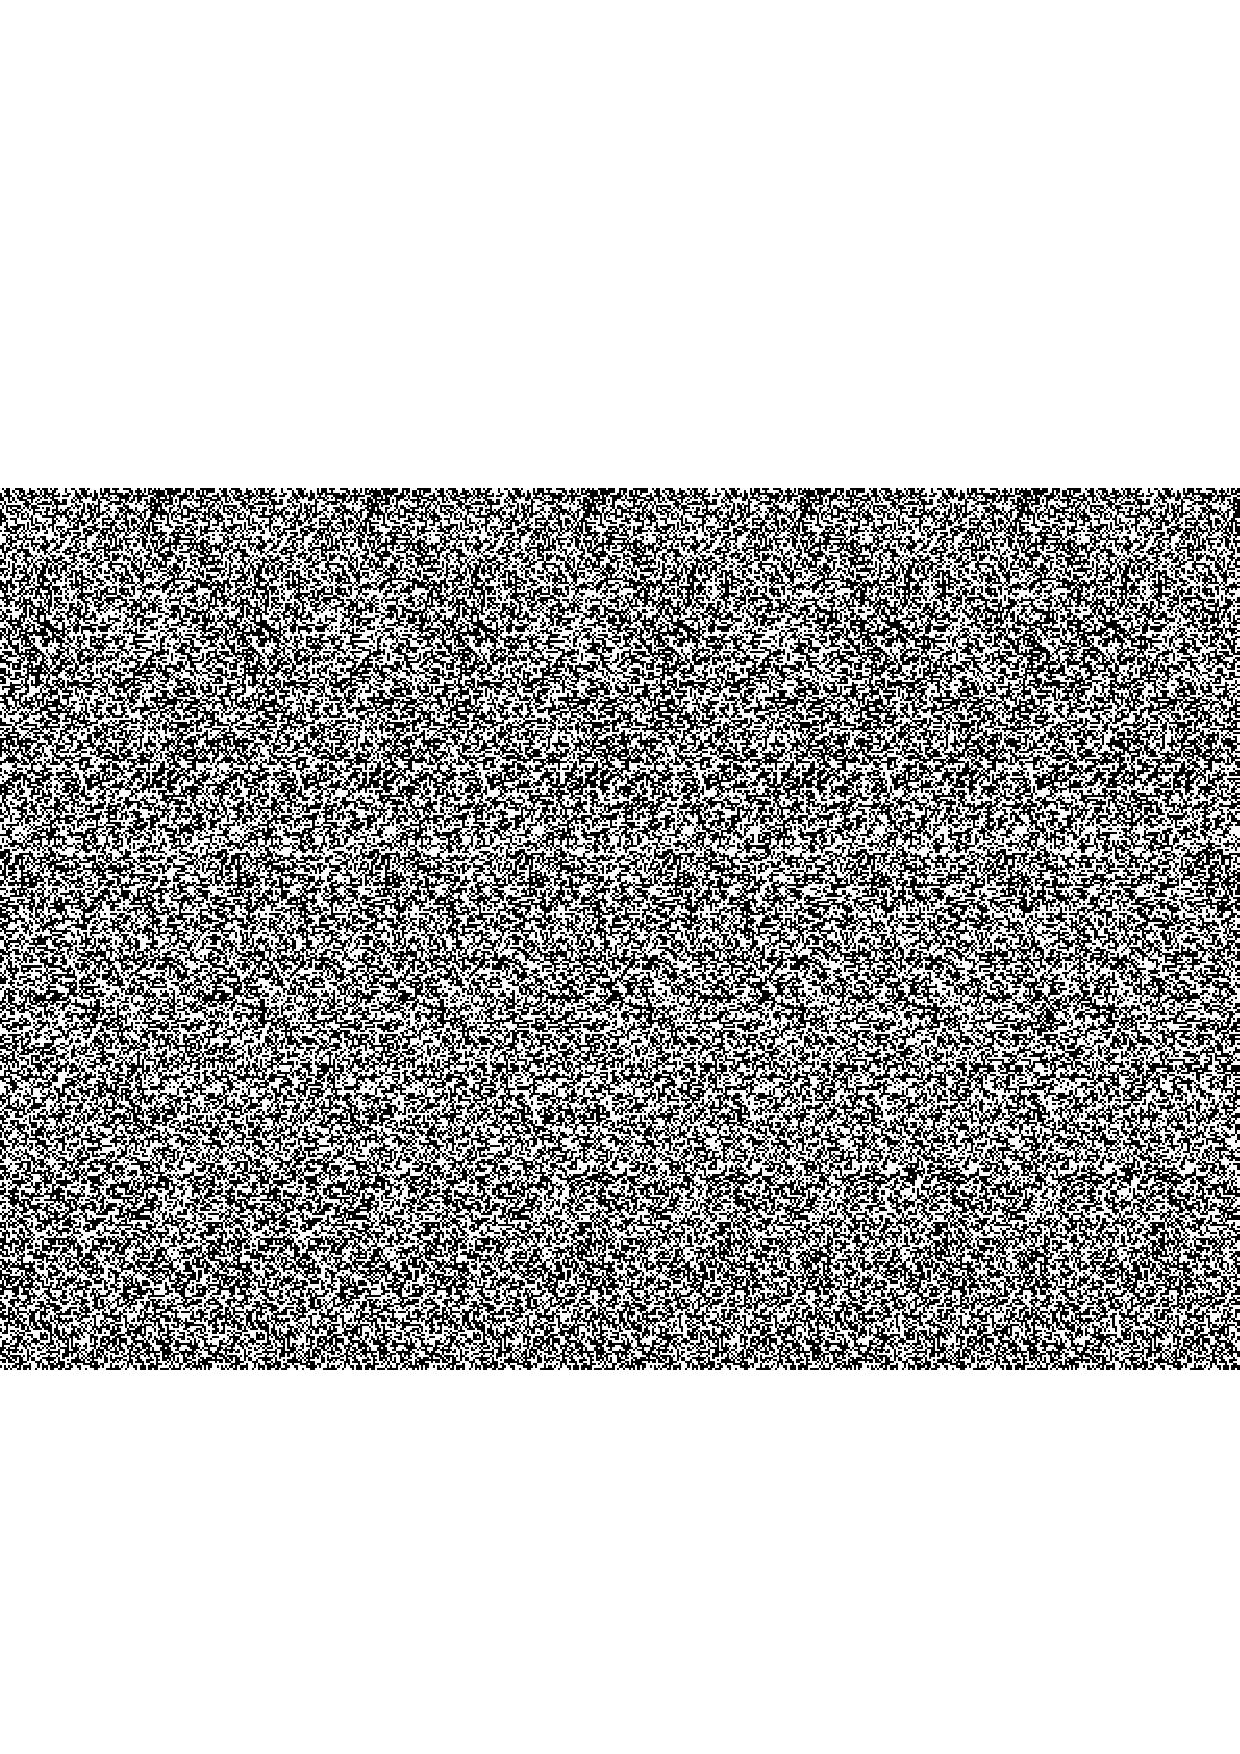
\includegraphics[scale=0.40]{noeudRDA}}
\end{figure}
\center{\bf{\Huge{ESPACES \hspace{0.4cm}FIBR\'ES}}}
\vspace{0.35cm}
\center{\bf{\huge{et}}}
\vspace{0.35cm}
\center{\bf{\Huge{CONNEXIONS}}}
\vspace{0.35cm}
\center{\bf{\Large{Une introduction aux g\'eom\'etries}}}
\center{\bf{\Large{ classiques et quantiques}}} 
\center{\bf{\Large{de la  physique th\'eorique}}}
\vspace{1.0cm}
\begin{flushleft}
{\LARGE {Robert Coquereaux}}\\
\vspace{0.15cm}
{\Large Centre de Physique Th\'eorique}\\
\vspace{0.1cm}
{\Large Luminy - Marseille}
\end{flushleft}
\end{titlepage}
%%%%%%%%%%%%%%%%%%%%%%%%%%%%%%%%%%%%
\bibliographystyle{plain}
\thispagestyle{empty}
A mes enfants Val\'erie, Eric et Rapha\"el
\maketitle
\clearemptydoublepage
\pagenumbering{roman}
\tableofcontents
\clearemptydoublepage
%%%%%%%%%%%%%%%%%%
\pagestyle{plain}
\chapter*{Pr\'eface}
\addcontentsline{toc}{chapter}{Pr\'eface}

Il est quelquefois plus facile de pr\'esenter un livre en disant ce 
qu'il n'est pas et en dressant une liste des motivations de
l'auteur qu'en essayant d'en expliciter le contenu.

Ce livre, bien qu'il contienne un expos\'e  de
g\'eom\'etrie diff\'erentielle (avec un accent particulier mis sur
les groupes de Lie, la th\'eorie des espaces fibr\'es, la th\'eorie
des connexions et la g\'eom\'etrie riemannienne) n'est certainement
pas un cours de math\'ematiques traditionnel. En g\'en\'eral les math\'ematiciens
cultivent
%d'ordinaire et \`a loisir,
 la pr\'ecision du
style et la concision du discours, alors que l'expos\'e qui suit  essaye
% au contraire 
de pr\'esenter les id\'ees importantes en faisant
souvent appel \`a l'intuition, en effectuant de nombreux retours en
arri\`ere et en ne n\'egligeant pas les clins d'oeil \`a la physique.
On peut donc esp\'erer que la lecture de l'ouvrage pr\'esent sera un
peu moins aride que celle d'un trait\'e traditionnel.
\par
Ce livre n'est pas non plus un cours de physique
th\'eorique. Il y manque beaucoup trop d'informations~! Celui ou
celle qui souhaite se lancer \`a la d\'ecouverte de l'Espace-Temps et
d\'echiffrer certains des myst\`eres de notre univers devrait
s'attaquer \`a de saines lectures (par exemple \cite{MTW}). 
L'ouvrage pr\'esent ressemble plus
\`a un cours de math\'ematiques qu'\`a un cours de physique; la
physique n'est cependant pas absente, au contraire: des id\'ees
physiques sont cach\'ees derri\`ere chaque paragraphe, et ce sont elles
qui sont, la plupart du temps, \`a l'origine des notions
``abstraites'' que nous allons pr\'esenter.
\par 

Bien qu'il ne s'agisse pas l\`a d'un ouvrage de vulgarisation sur la
physique th\'eorique ou les math\'ematiques, j'ai pourtant
r\'edig\'e de nombreux paragraphes en pensant \`a certains de mes amis
%poss\'edant
ayant une culture math\'ematique relativement modeste mais
n\'eanmoins dot\'es d'un esprit curieux et aimant vagabonder de temps
\`a autres sur des terrains situ\'es au confluent de l'infiniment
petit, de l'infiniment grand, des math\'ematiques et de la
m\'etaphysique. Je dois dire, en relisant l'ouvrage apr\`es coup,
que, de ce point de vue, j'ai peur d'avoir echou\'e: le contenu
pr\'esent\'e ressemble plus \`a un cours de troisi\`eme cycle
sp\'ecialis\'e qu`\`a un ouvrage de vulgarisation$\ldots$
 Cela dit, je pense --- et j'esp\`ere --- qu'\`a la condition de commencer
la lecture \`a la premi\`ere page sans essayer de d\'emarrer en plein milieu,
l'ouvrage reste accessible \`a tout lecteur disposant d'un bagage math\'ematique
\'equivalent \`a celui qu'on est cens\'e acqu\'erir \`a l'issue d'un premier cycle universitaire,  ou d'une 
classe de Math\'ematiques Sp\'eciales.
A propos de motivations, je dois aussi
signaler que d'autres de mes amis, dot\'es d'une culture
math\'ematique plus que respectable n'ont malheureusement jamais eu
le temps ou la patience de traduire le jargon quelquefois flou des
physiciens dans la langue bourbakiste qu'ils affectionnent. Le
pr\'esent ouvrage, bien que r\'esolument peu bourbakiste dans le
style, est \'egalement \'ecrit pour eux. Finalement, ce livre est
\'egalement ---et probablement surtout--- \'ecrit pour les
\'etudiants en math\'ematiques ou en physique, mais qu'on ne vienne pas
me demander ``De quelle ann\'ee?''~!
En effet, certains des th\`emes qui seront abord\'es peuvent \^etre rencontr\'es dans un
cours de ma\^itrise de math\'ematiques (ou de DEA) et on les
trouvera souvent incorpor\'es \`a un enseignement de troisi\`eme cycle
de physique th\'eorique ou de g\'eom\'etrie diff\'erentielle, 
mais d'autres th\`emes, probablement aussi int\'eressants, et quelquefois m\^eme fondamentaux, risquent fort de ne figurer dans le programme d'aucun enseignement universitaire.
L'\'etudiant, physicien ou
math\'ematicien, trouvera peut-\^etre, dans cet ouvrage, ce qu'il
cherche (en utilisant l'index et la table des mati\`eres) et le
non-sp\'ecialiste y trouvera peut-\^etre ce qu'il ne cherchait pas$\ldots$ \par

Enfin, ce livre n'est pas un ouvrage de philosophie ou de
m\'etaphysique (Dieu m'en garde!) bien que certaines r\'eflexions de
nature \'eminemment philosophiques ne soient pas absentes des pages
qui suivent, surtout dans la section Introduction.\par

La partie ``g\'eom\'etrie diff\'erentielle''  de ce travail est issue d'un
cours de troisi\`eme cycle que j'ai eu l'occasion de donner pendant plusieurs
ann\'ees au sein du Dipl\^ome d'Etudes Approfondies (DEA) de Physique
Th\'eorique, organis\'e au Centre de Physique Th\'eorique, \`a Luminy (Marseille) ainsi qu'en 1997, dans le DEA de Physique Th\'eorique organis\'e \`a 
l'Ecole Normale Sup\'erieure de Lyon. La partie ``non commutative'' (la derni\`ere section) est un court extrait d'une s\'erie de cours que j'ai  donn\'es dans les universit\'es de Rio de Janeiro (URJ, UFRJ et CBPF), de Saragosse et de La Plata ainsi qu'\`a San Carlos de  Bariloche, en 1996 et 1997. L'ouvrage a \'egalement servi de support \`a un cours semestriel de l'IMPA, Rio de Janeiro, en 2012 (P\'os-Gradua\c c\~ao em Matem\'atica, curso de Doutorado).



\clearemptydoublepage

\chapter*{Introduction}
\addcontentsline{toc}{chapter}{Introduction}
\section*{\sl Mod\`eles math\'ematiques et r\'ealit\'e}
\addcontentsline{toc}{section}{Mod\`eles math\'ematiques et r\'ealit\'e}

Qu'est ce que la ``R\'ealit\'e''? Existe-t-elle seulement? Que
signifie le verbe ``exister'' de la proposition
interrogative pr\'ec\'edente? Que le lecteur allergique aux
discussions philosophiques se rassure, nous n'allons pas
continuer longtemps dans cette direction. Cependant, pour
ne pas nous enliser dans de faux probl\`emes s\'emantiques et
pour bien appr\'ecier en quel sens nous comprenons ou
pr\'etendons comprendre les ph\'enom\`enes naturels (y en a-t-il
qui ne le soient pas?) il nous faut apporter une r\'eponse
pragmatique aux questions pr\'ec\'edentes et tenter de d\'efinir
les mots eux-m\^emes que nous utilisons.\par
Le point de vue adopt\'e par l'auteur est le
suivant:\par

$\bullet$ Il est impossible de donner une signification
quelconque \`a la phrase suivante: La R\'ealit\'e est.
L'auteur croit cependant en l'existence d'une r\'ealit\'e
objective dont la nature est ind\'ependante de l'analyse
qui peut en \^etre faite. Malheureusement, il s'av\`ere
\'egalement impossible de donner un sens raisonnable \`a
l'assertion pr\'ec\'edente. La croyance de l'auteur est donc
un acte de foi au sens m\'etaphysique du terme. On pourra
donc utiliser le mot ``ph\'enom\`ene'' comme
synonyme du mot ``r\'ealit\'e'', le vocable en question \'etant
lui-m\^eme non d\'efini. \par

$\bullet$ La description d'un ph\'enom\`ene, quel qu'il soit,
fait toujours appel aux math\'ematiques, m\^eme si le spectateur n'en est
pas conscient. Ainsi, d\'eclarer que deux individus font
partie de la m\^eme lign\'ee (au sens h\'er\'editaire du terme)
signifie qu'on assimile --peut \^etre inconsciemment-- les
individus en question aux \'el\'ements d'un ensemble sur
lequel on a d\'efini une  relation d'ordre partiel.
De la m\^eme fa\c con, la travers\'ee d'un terrain par un ballon
de foot-ball est un ph\'enom\`ene admettant une description
(en fait plusieurs) dont la nature est essentiellement
math\'ematique. Par exemple, on peut consid\'erer la
trajectoire d'un point traversant un rectangle en ligne
droite. Il existe cependant une description du m\^eme
ph\'enom\`ene ou le ballon n'est plus un point mais une sph\`ere
et ou le terrain n'est plus assimil\'e \`a un rectangle mais
une figure g\'eom\'etrique plus complexe (coins plus ou moins
arrondis, c\^ot\'es plus ou moins parall\`eles etc.) On peut
d'ailleurs continuer dans ce sens et tenir en compte
l'existence de creux et de bosses sur la surface du
ballon, de la couleur etc. Les humains n'ont pas besoin
de suivre des cours de math\'ematiques sup\'erieures pour
appr\'ecier un match de foot-ball, mais il est important de
constater l'aptitude de l'esprit \`a cr\'eer
inconsciemment des mod\`eles math\'ematiques relativement
\'elabor\'es pour analyser l'exp\'erience quotidienne. Notons
enfin qu'un ph\'enom\`ene donn\'e poss\`ede d'ordinaire plusieurs
descriptions math\'ematiques (et m\^eme une infinit\'e).\par

$\bullet$ La croyance en l'existence d'une r\'ealit\'e objective
n'a aucune importance pratique; seule compte
l'ensemble de ses descriptions math\'ematiques.
 En effet, lors de l'analyse d'un
ph\'enom\`ene (la travers\'ee de la cour par un ballon de
foot-ball), nous pouvons adopter les deux points de vue
suivants. 1) La travers\'ee de la dite cour par le ballon en
question est un ph\'enom\`ene ``r\'eel'' dont nous pouvons
donner une quantit\'e de descriptions math\'ematiques
compatibles, et il est d'ailleurs possible de pr\'eciser la notion de
compatibilit\'e des descriptions. 2) La travers\'ee de la
dite cour par le ballon en question est en fait {\sl
d\'efinie} par un ensemble (infini) de descriptions
math\'ematiques compatibles. Peu importe que nous adoptions
l'un ou l'autre de ces deux points de vue, car si un
aspect d'un ph\'enom\`ene n'est pas math\'ematiquement
mod\`elisable, cet aspect rel\`eve --presque par d\'efinition-- de la
m\'etaphysique et il n'est pas clair qu'on puisse y
attribuer un sens (m\^eme si on a envie de croire sans
comprendre). On peut se convaincre du fait que l'exercice classique
de m\'editation sur le th\`eme de la chaise (Quelle est
cette chaise? Quelle est sa fonction? Quelle est sa nature?
Quelle est son histoire? etc.) est compl\`etement
mod\`elisable en termes math\'ematiques...\par


Pour nous, un ph\'enom\`ene est donc d\'efini par l'ensemble de ses
descriptions math\'ematiques. Du point de vue linguistique, on
devrait peut-\^etre distinguer en g\'en\'eral le ph\'enom\`ene lui-m\^eme
(concept assez flou) de sa description math\'ematique -- ou plut\^ot,
de ses descriptions math\'ematiques. On peut alors parler de
mod\'elisation du ph\'enom\`ene, mais il faut bien voir que c'est la
mod\'elisation elle-m\^eme qui rend le ph\'enom\`ene accessible \`a
l'analyse. Le mod\`ele math\'ematique, qu'il soit choisi consciemment
(par un physicien, par exemple) ou inconsciemment (par exemple, par un
spectateur du match) apporte avec lui son propre langage, c'est \`a
dire les mots qui permettent \`a l'observateur de se poser des
questions \`a propos du ph\'enom\`ene qu'il contemple. Chacun de ces
mots est cens\'e \^etre susceptible d'une traduction math\'ematique
pr\'ecise dans un cadre formel --- que l'observateur ne d\'efini pas
n\'ecessairement --- faute de quoi, les mots en question sont simplement
vides de sens. Il faut bien \^etre conscient du fait que la phrase
``mais que se passe-t-il vraiment?'' pos\'ee par le profane
repose sur la croyance en une r\'ealit\'e objective, r\'ealit\'e qui,
de notre point de vue, \'echappe \`a toute analyse scientifique.\par
Qu'en est-il donc de la distinction entre physique et
math\'ematiques? Pour nous, dire qu'une figure dessin\'ee sur une
feuille de papier est un triangle, c'est ``faire de la physique'': le
triangle est une notion abstraite appartenant au
monde des math\'ematiques, associer cette notion au dessin qu'on
a sous les yeux est un travail de physicien. Dans un genre
diff\'erent, supposons qu'on fabrique des ``choses'' avec un canon
\`a \'electrons$\ldots$ qu'est ce donc qu'un \'electron? On peut dire
que c'est une petite boule, on peut dire que c'est une fonction
(complexe) --une onde~!--, on peut dire que c'est une section d'un
certain espace fibr\'e vectoriel (un ``champ de Dirac'') ou que c'est un
\'el\'ement d'un module projectif de type fini sur une alg\`ebre non
n\'ecessairement commutative$\ldots$ Toutes ces descriptions sont
math\'ematiques et la premi\`ere (la boule) est la plus simple du
point de vue du bagage math\'ematique utilis\'e mais toutes ces
descriptions sont \'egalement ``vraies'' et apportent avec elles
leur propre langage. Il y a des questions qu'on ne peut poser
qu'apr\`es avoir {\it choisi} une certaine description. C'est ainsi
que les math\'ematiques sont n\'ecessaires \`a la description de ce
que nous appelons les ph\'enom\`enes naturels (cons\'equence
imm\'ediate: si vous avez des difficult\'es en physique, c'est que
vous n'avez pas proprement assimil\'e les math\'ematiques
n\'ecessaires!). La physique consiste essentiellement \`a habiller le
ph\'enom\`ene de notre choix avec des math\'ematiques appropri\'ees et
c'est cet habillage qui rend les choses accessibles au discours.
C'est l\`a quelque chose qu'il ne faut pas oublier mais il faut
avouer qu'il est n\'eanmoins commode de vivre en faisant ``comme si'' on
croyait \`a l'existence d'une r\'ealit\'e objective! On pourrait
aussi passer au cran sup\'erieur et se demander si les
math\'ematiques elles-m\^emes ``existent''. Il n'est pas clair que la
phrase ait un sens mais il est certain que, de la m\^eme fa\c con
qu'il est commode de croire en l'existence d'une r\'ealit\'e physique
objective, il est \'egalement commode de  croire en l'existence d'une
r\'ealit\'e math\'ematique qu'il s'agit pour nous de d\'ecouvrir
(comme un explorateur dans la jungle ou comme un physicien
exp\'erimentateur).
Les chapitres qui suivent pr\'esentent des concepts math\'ematiques.
Ind\'ependamment de la beaut\'e ou de l'\'el\'egance intrins\`eque
des concepts en question, nous voulons attirer l'attention du
lecteur (m\^eme s'il n'est pas physicien) sur le fait que ces
concepts jouent un r\^ole majeur dans l'``habillage'' contemporain des
th\'eories physiques,  et que, dans de nombreux cas, ces concepts
sont eux-m\^emes issus de consid\'erations relevant de la physique
th\'eorique.

\section*{Du classique au quantique: math\'ematiques commutatives et non commutatives}
\addcontentsline{toc}{section}{Du classique au quantique}

 Avant d'arr\^eter l\`a ces consid\'erations
\'epist\'emologiques pour passer \`a notre premier chapitre
consacr\'e \`a l'\'etude des vari\'et\'es diff\'erentiables, nous
voulons dire un mot sur la distinction entre physique classique et
physique quantique, en parall\`ele avec la distinction entre 
``math\'ematiques commutatives'' et ``math\'ematiques non
commutatives''. Cette remarque risque de n'\^etre comprise que par
les lecteurs ayant d\'ej\`a une certaine familiarit\'e avec les
sujets mentionn\'es mais le lecteur int\'eress\'e pourra peut-\^etre
relire ce commentaire en y revenant un peu plus tard.
Les math\'ematiques commutatives (la g\'eom\'etrie commutative en
particulier) s'occupe des propri\'et\'es math\'ematiques des
``espaces'' (th\'eorie de la mesure, espaces topologiques,
diff\'erentiables, riemanniens, homog\`enes, poss\'edant une
structure de groupe$\ldots$) Pour le physicien, ces espaces
fournissent un mod\`ele math\'ematique concernant le syst\`eme qu'il a
choisi d'\'etudier et toutes les quantit\'es qui l'int\'eressent
peuvent \^etre d\'ecrites \`a l'aide d'une classe appropri\'ee de
fonctions d\'efinies sur de tels espaces. Il se trouve que les
propri\'et\'es des espaces en question peuvent elles-m\^emes \^etre
cod\'ees en termes des propri\'et\'es de ces alg\`ebres de
fonctions; il s'agit l\`a d'un r\'esultat profond dont l'expression
pr\'ecise est due \`a Gelfand (voir chapitre 6). Le vocable ``math\'ematiques
commutative'' vient du fait que toutes ces alg\`ebres sont des
alg\`ebres commutatives pour les lois d'addition et de multiplication
des fonctions. Attention, de ce point de vue, la th\'eorie des
groupes de Lie (voir plus loin) --groupes qui ne sont pas, en
g\'en\'eral, commutatifs-- fait partie des ``math\'ematiques
commutatives'' car l'alg\`ebre des fonctions (\`a valeurs r\'eelles
ou complexes) d\'efinie sur un groupe est une alg\`ebre commutative !
Les ``math\'ematiques non commutatives'', au contraire, s'occupent des
propri\'et\'es d'alg\`ebres qui ne sont pas commutatives et des
objets qui g\'en\'eralisent les constructions usuelles lorsqu'on
remplace les alg\`ebres de fonctions (et les ``espaces'' eux-m\^emes)
par des alg\`ebres d'op\'erateurs. Les quantit\'es qui int\'eressent
le physicien ne sont plus alors cod\'ees par des fonctions
num\'eriques mais, typiquement, par des op\'erateurs agissant dans
des espaces hilbertiens. Il est inutile d'en dire plus \`a ce niveau
mais nous effectuerons deux remarques. La premi\`ere est
terminologique: un physicien dit qu'il fait de la physique classique
lorsqu'il utilise des math\'ematiques commutatives pour d\'ecrire un
ph\'enom\`ene (ce qui, philosophiquement, revient \`a le d\'efinir !
Voir la discussion pr\'ec\'edente)  et de la physique quantique
lorsqu'il utilise des math\'ematiques non commutatives (idem).
 La seconde remarque a trait au contenu de cet ouvrage: il
traite de g\'eom\'etrie, et la plupart du temps de g\'eom\'etrie
utilis\'ee en physique fondamentale, cependant il s'agira presque
toujours de g\'eom\'etrie commutative, vocable englobant d'ailleurs
toute la g\'eom\'etrie, au sens usuel du terme, qu'elle soit
euclidienne ou non. Du point de vue de la physique, nos
constructions correspondront donc \`a des constructions de th\'eorie
classique des champs (m\^eme s'il nous arrive de parler de quarks ou
d'\'electrons de Dirac) et non de th\'eorie quantique des champs.
\par
Le dernier chapitre est une introduction aux ``math\'ematiques non 
commutatives'' (un point de vue assez particulier sur la th\'eorie 
des alg\`ebres associatives) et pr\'esente  
quelques notions fondamentales relevant de le g\'eom\'etrie 
diff\'erentielle non commutative. Ce dernier chapitre pourrait donc 
aussi s'intituler : Introduction \`a la {\sl g\'eom\'etrie quantique\/}.
\vfill
\eject

\section*{Guide de lecture, autocritique et perspectives}
\addcontentsline{toc}{section}{Guide de lecture, autocritique et perspectives}

Le lecteur ne connaissant rien au sujet et d\'esirant ``se faire une id\'ee'',
peut dans un premier temps,
parcourir les sections 1.1, 1.2, 2.1, 2.2.1, ainsi que
3.1, (3.2.1 $\rightarrow$ 
3.2.5), 3.3.1, 3.3.2,  (4.1.1 $\rightarrow$ 4.1.4)  et (4.4.1, 5.6.1, 6.1, 6.2.1, 
6.3.1) dont le contenu, 
\`a peu pr\`es exempt de 
formules, fait appel \`a 
l'intuition et ne suppose que tr\`es peu de connaissances 
pr\'ealables.

\bigskip
Les autres sections sont assez in\'egales ; certaines pr\'esentent un mat\'eriel 
qui fait ou devrait faire partie du
bagage math\'ematique standard de tout math\'ematicien ou physicien th\'eoricien,
certaines autres sont d'un niveau plus avanc\'e et peuvent contenir des 
informations qui ne sont pas n\'ecessairement disponibles ailleurs (sauf 
peut-\^etre dans quelques articles sp\'ecialis\'es).
En fait, comme le titre l'indique, le but initial de ce travail \'etait de
fournir une pr\'esentation  --- si possible p\'edagogique --- des espaces
fibr\'es et de la th\'eorie des connexions. Il se trouve que certains lecteurs
potentiellement int\'eress\'es, en particulier les \'etudiants de
troisi\`eme cycle de physique th\'eorique, n'ont souvent pas, au d\'epart, les 
bases math\'ematiques n\'ecessaires pour attaquer, de front, un cours 
relativement complet sur les espaces fibr\'es : il leur manque souvent un
cours pr\'ealable de calcul diff\'erentiel sur les vari\'et\'es et un cours sur
les groupes de Lie. C'est la raison d'\^etre des parties $1$ et $2$ de cet
ouvrage. On a essay\'e d'y pr\'esenter les notions indispensables \`a la
lecture des chapitres $3$ et $4$ consacr\'es aux espaces fibr\'es et 
\`a la th\'eorie des connections. Nous sugg\'erons donc \`a ceux qui ont d\'ej\`a
acquis une formation raisonnable en ce qui concerne les vari\'et\'es 
diff\'erentiables (par exemple en lisant
le premier volume de \cite{Spivak}
et les groupes de Lie, de jeter d'abord un coup d'\oe{il} au
sommaire, puis de sauter les deux premiers chapitres --- qui
ne leur apprendront sans doute pas grand chose --- et 
d'entamer directement la lecture de cet ouvrage au chapitre $3$.
Pour les autres$\ldots$ il vaudrait peut-\^etre mieux 
s'astreindre \`a lire les diff\'erentes parties dans l'ordre.
Comme nous l'avons mentionn\'e dans la pr\'eface,
l'ensemble de l'ouvrage devrait
\^etre lisible par  quelqu'un ne disposant pas d'un bagage math\'ematique
sup\'erieur \`a celui qu'on acquiert d'ordinaire, ou qu'on est sens\'e acqu\'erir,  en premier cycle.
Son contenu, n\'eanmoins, serait plut\^ot d'un niveau $3^{\grave{e}me} 
\, cycle$. 

Le plan et la structure de ce livre r\'epond \`a la pr\'eoccupation suivante : 
faire du lecteur un ``honn\^ete homme'' en g\'eom\'etrie diff\'erentielle 
classique en pr\'esentant un certain nombre de notions qui sont 
fr\'equemment utilis\'ees en physique th\'eorique ou en math\'ematiques. Savoir si le but sera atteint est une 
autre histoire$\ldots$ Enfin, et au risque de faire hurler certains
math\'ematiciens, il nous semble plus important, tout au moins dans un premier temps, de se familiariser avec les 
id\'ees fondamentales ainsi qu'avec de nombreux exemples, que de conna\^itre
le d\'etail de toutes les d\'emonstrations relatives aux propositions et 
th\'eor\`emes cit\'es. 


Le style adopt\'e dans ce livre \'etant volontairement informel, il 
peut \^etre parfois difficile au lecteur de retrouver la d\'efinition 
pr\'ecise de tel ou tel concept. Pour cette raison, il peut \^etre 
utile de consulter l'index situ\'e en fin d'ouvrage, et, bien 
entendu, la table des mati\`eres.

Notre pr\'esentation est bien, sur, incompl\`ete. Certains aspects ne sont qu'effleur\'es,
d'autres sont totalement absents et bien qu'il ne s'agisse pas 
ici, loin s'en faut, d'une tentative encyclop\'edique, voici
quelques t\^etes de chapitres dont
on pourra d\'eplorer l'absence$\ldots$ :
compl\'ements de g\'eom\'etrie diff\'erentielle \'el\'ementaire en 
basse dimension (la liste serait longue),
g\'eom\'etrie symplectique et m\'ecanique, 
op\'erateurs diff\'erentiels, pseudo-diff\'erentiels, symboles etc.,
\'etude des \'equations de Yang-Mills, instantons etc.,
classification des espaces fibr\'es, fibr\'es universels et espaces classifiants,
K-th\'eorie,
classes caract\'eristiques (et classes caract\'eristiques secondaires),
g\'eom\'etries sur les groupes de Lie et les espaces 
homog\`enes,
applications harmoniques,
aspects conformes,
m\'etriques et connexions invariantes (sym\'etries, isom\'etries),
vari\'et\'es complexes, hypercomplexes etc.,
g\'eom\'etrie de l'espace des orbites des connexions,
g\'eom\'etrie de l'espace des m\'etriques,
etc.


Par ailleurs, l'auteur aurait aim\'e ins\'erer, \`a la fin de chaque 
chapitre, une section consacr\'ee aux g\'en\'eralisations des id\'ees
rencontr\'ees, lorsqu'on passe de la g\'eom\'etrie commutative \`a la g\'eom\'etrie
non commutative, c'est \`a dire lorsqu'on passe du classique au quantique\footnote{Mentionnons
\`a ce propos le trait\'e \cite{ACbook} qui restera sans
doute pour longtemps l'ouvrage de r\'ef\'erence en g\'eom\'etrie non
commutative.}.
Il est sans doute dommage de devoir parler au conditionnel pass\'e$\ldots$
mais il fallait bien mettre fin \`a la r\'edaction ! 
De fait, faisant suite \`a une premi\`ere version de cet ouvrage, rendue 
disponible sur Internet, en format html, en mai 1997, la derni\`ere 
section (section 6), consacr\'ee \`a une pr\'esentation g\'en\'erale 
des math\'ematiques non commutatives et au calcul diff\'erentiel sur 
les alg\`ebres non commutatives, a \'et\'e rajout\'ee  en mars 1998. Ce 
rajout r\'epond donc, en partie, \`a la pr\'eoccupation mentionn\'ee plus haut.

 Bien entendu, toutes les remarques permettant d'am\'eliorer ce 
 document, voire de corriger certaines sections si besoin est, sont les 
 bienvenues : envoyer un courrier \`a l'auteur ou un courriel 
\`a coque at cpt.univ-mrs.fr.

On aura compris que ce livre a \'et\'e r\'edig\'e en fran\c cais. 
Certes, il eut \'et\'e pr\'ef\'erable, pour rassembler un plus large lectorat, de r\'ediger directement l'ouvrage en anglais.
L'usage de la langue anglaise, et en particulier la lecture de l'anglais, sont devenus obligatoires dans notre soci\'et\'e, et il est certain que l'enseignement de cette langue a fait des progr\`es consid\'erables en France; il n'en demeure pas moins que la lecture de textes en anglais, m\^eme de textes scientifiques, pose toujours \`a nos \'etudiants ainsi qu'\`a certains de leurs a\^in\'es, des difficult\'es.
Il en va d'ailleurs de m\^eme pour une vaste partie du monde francophone, o\`u le fran\c cais n'est parfois qu'une deuxi\`eme langue (l'anglais venant en troisi\`ieme position).
Il n'est pas certain que le pr\'esent ouvrage devienne un livre de chevet (!) mais pour faciliter sa lecture sans rajouter une difficult\'e linguistique, l'auteur a d\'ecid\'e de r\'ediger ce livre directement en fran\c cais. 
Ces notes sont donc  d\'edi\'ees aux \'etudiants et aux chercheurs de la francophonie, et \`a tous les esprits curieux qui souhaitent acqu\'erir un certain nombre de notions g\'eom\'etriques des math\'ematiques contemporaines avant de s'embarquer eux-m\^emes dans l'aventure de la recherche, que ce soit en Physique ou en Math\'ematique, ou qui souhaitent tout simplement satisfaire leur curiosit\'e intellectuelle.
Une version anglaise serait la bienvenue mais l'auteur n'a pas eu,  jusqu'\`a pr\'esent, le courage de s'atteler \`a cette t\^ache.


\section*{\sl Disponibilit\'e}

L'ensemble du document (sa derni\`ere version) est accessible,
via internet, en version html ou pdf sur \url{http://www.cpt.univ-mrs.fr/~coque/}.
% via internet, en version html ou postscript sur $http://www.cpt.univ-mrs.fr/\tilde{}coque/$.
% et est \'egalement  disponible, en version papier, 
% sous forme d'un rapport CNRS reli\'e (contacter Mme M. Rossignol, 
% CPT-CNRS, case 907, Luminy, 13288, Marseille, ou, par e-mail
% michele at cpt.univ-mrs.fr).

\vfill
\eject

\section*{\sl Bibliographie}

On trouvera assez peu de r\'ef\'erences mentionn\'ees dans
cet ouvrage. Il existait \'evidemment la tentation de citer tous les
livres traitant, de pr\`es ou de loin, de g\'eom\'etrie diff\'erentielle,
d'espaces fibr\'es, de connexions, de  g\'eom\'etrie riemannienne \etc.
Un tel effort bibliographique semble \'evidemment, d\`es le d\'epart, vou\'e \`a
l'\'echec. Une autre solution e\^ut \'et\'e de ne citer que les ouvrages
\'el\'ementaires. Malheureusement, les ouvrages en question
 ne recouvrent pas
 n\'ecessairement tous les sujets qui sont abord\'es ici.
 Enfin, on rappelle que la premi\`ere r\'edaction de ces notes, avant leur mise \`a disposition sur internet, date de 1996; 
 plusieurs ouvrages d'enseignement sur des sujets voisins sont apparus depuis.
 L'attitude que nous avons choisi d'adopter est de ne citer que les livres
 et autres travaux pour lesquels l'auteur a conscience d'avoir subi
 une influence possible ou certaine. 
 Les documents en question sont assez vari\'es :
 certains sont des ouvrages de r\'ef\'erence, d'autres sont des 
 monographies sp\'ecialis\'ees, d'autres encore, des articles de recherche.
 L'auteur n'a pas cherch\'e \`a suivre tel ou tel trait\'e et a essay\'e de r\'ediger
 ces notes de fa\c con originale$\ldots$ certains pourront peut-\^etre s'en plaindre !
 Tout ceci explique la raison du petit nombre de r\'ef\'erences, que voici. 

\vfill\eject




\bibliography{biblio}
\clearemptydoublepage
\addcontentsline{toc}{chapter}{}
\pagestyle{headings}
\pagenumbering{arabic}


\chapter {Vari\'et\'es diff\'erentiables}
\minitoc

\section {Vari\'et\'es topologiques}

\subsection  {D\'efinition}
\par
Une {\sl vari\'et\'e topologique}\index{vari\'et\'e topologique} est tout d'abord un espace
topologique, mais on suppose, de surcro\^{i}t, que chacun de
ses points poss\`ede un voisinage hom\'eomorphe \`a un ouvert
de $\RR^n$. On dit alors que cet espace est une vari\'et\'e
topologique de dimension~$n$.\par

Intuitivement, une vari\'et\'e topologique de dimension $2$
est un espace qui, localement, c'est \`a dire si on ne
regarde pas trop loin, ressemble \`a un petit morceau de
feuille de papier qu'on aurait pu d\'ecouper avec des
ciseaux apr\`es en avoir trac\'e le pourtour au crayon (on
peut d'ailleurs froisser le bout de papier en question).
La structure globale de cet espace peut \^etre \'evidemment
assez diff\'erente puisque la vari\'et\'e elle-m\^eme est obtenue
par recollement de tous ces petits morceaux de papier.
Ainsi, un pneu de bicyclette, \'eventuellement d\'egonfl\'e,
pli\'e et ``froiss\'e'' fournit un exemple d'objet physique
qu'on peut mod\'eliser \`a l'aide d'une vari\'et\'e topologique de
dimension $2$: un tore.
\smallskip
\subsection  {Vari\'et\'es \`a bord}
\par
 Les vari\'et\'es dont il vient d'\^etre question n'ont pas de
bord (au sens intuitif du terme). En effet, si nous nous
transformons en \^etres plats, rampant sur la surface d'un
ballon -- ou d'un pneu -- nous ne sommes jamais arr\^et\'es
par une quelconque barri\`ere. Cela ne serait pas le cas si
nous nous d\'eplacions sur la surface d'un quartier d'orange
ou d'un pneu crev\'e (nous nous arr\^eterions au bord du
trou!). Sans se transformer en \^etres plats, cela ne serait
pas le cas non plus si nous nous d\'eplacions \`a l'int\'erieur
d'une boule ferm\'ee. De fa\c con g\'en\'erale, il est possible de
fabriquer des ``vari\'et\'es \`a bord'' en effectuant un ou
plusieurs trous dans une vari\'et\'e sans bord (\`a l'aide d'une
petite cuill\`ere multi-dimensionelle!); la partie enlev\'ee,
comme la partie qui reste, devient une {\sl vari\'et\'e topologique \`a 
bord\/}.\par

Pour pr\'eciser cette notion, il nous faut \'elargir la
d\'efinition de vari\'et\'e que nous avons donn\'e plus
haut puisque certains des points (ceux du bord) ont un
voisinage non pas hom\'eomorphe \`a un ouvert de $\RR^n$ mais \`a\
un voisinage de $\RR^n_+$ (le ferm\'e de $\RR^n$  form\'e des points dont
la derni\`ere composante est positive ou nulle).
\par

Attention: si nous nous promenons dans une boule
ouverte, nous ne pourrons jamais atteindre aucun bord... par
d\'efinition d'une boule ouverte! Une boule ouverte est une
vari\'et\'e sans bord de dimension $3$ qui est d'ailleurs
hom\'eomorphe \`a $\RR^3$. Par contre, une boule ferm\'ee est une
vari\'et\'e \`a bord de dimension $3$, les points du bords sont
ceux de la sph\`ere (une vari\'et\'e de dimension $2$) et ils
poss\`edent -- dans la boule ferm\'ee -- des voisinages
particuliers. Le disque ouvert (la
boule de dimension $2$) est aussi une vari\'et\'e sans bord
et le disque ferm\'e est une vari\'et\'e \`a bord (son bord est
constitu\'e d'un cercle qu'on peut appeler \'egalement
``sph\`ere de dimension $1$''. Dans le m\^eme genre, un
intervalle ouvert est une vari\'et\'e sans bord (la boule de
dimension $1$) et un intervalle ferm\'e est une vari\'et\'e \`a
bord (son bord est constitu\'e de deux points dont la
r\'eunion constitue ce qu'on peut appeler la sph\`ere de
dimension $0$. Les exemples qui pr\'ec\`edent sont
g\'en\'eralisables en toutes dimensions.\par

Terminologie: Si on ne pr\'ecise pas davantage, une vari\'et\'e
topologique est cens\'ee \^etre une vari\'et\'e sans bord.\par
\smallskip
\subsection  {Contre-exemples}
\par
 La plupart des objets math\'ematiques auxquels nous avons
tendance \`a penser de prime abord sont des exemples de
vari\'et\'es topologiques (avec ou sans bord), et, pour cette
raison, il est bon de donner quelques exemples d'espaces
topologiques qui ne sont pas des vari\'et\'es.
 Consid\'erez par exemple une croix  (r\'eunion de
deux segments d'intersection r\'eduite \`a un point); ce n'est pas une vari\'et\'e 
car le point
situ\'e \`a l'intersection des deux segments poss\`ede des
voisinages en forme de croix, et une croix n'est jamais
hom\'eomorphe \`a un ouvert de $\RR = \RR^1$.  Le globe imp\'erial
est un objet qu'on pourrait penser \`a
mod\'eliser math\'ematiquement par une sph\`ere
(vari\'et\'e de dimension $2$) sur laquelle on aurait coll\'e
une croix (r\'eunion de deux segments) Cet espace n'est pas
une vari\'et\'e pour deux raisons. La premi\`ere vient du point
d'intersection des deux branches de la croix (d\'ej\`a vu) et
la deuxi\`eme est analogue puisque le point ou on a coll\'e
la croix sur la sph\`ere poss\`ede des voisinages qui ne sont
hom\'eomorphes ni \`a des ouverts de $\RR^1$ ni \`a des ouverts
de $\RR^2$. \par

Ces derniers exemples ne sont pas des vari\'et\'es mais sont
n\'eanmoins obtenus par recollement de vari\'et\'es... (CW
complexes) Ils ne poss\`edent pas une dimension
d\'etermin\'ee mais ont n\'eanmoins une structure assez
simple. On peut cependant faire bien pire... Les exemples
d'espaces topologiques qui ne sont pas des vari\'et\'es
abondent (prenez par exemple des espaces topologiques
qui ne sont pas de Haussdorf, c'est \`a dire qui poss\`edent
des points qu'on ne peut pas s\'eparer \`a l'aide d'ouverts
disjoints). Il ne faudrait pas croire que les espaces
qui ne sont pas des vari\'et\'es n'ont pas d'int\'er\^et
math\'ematique ou physique, bien au contraire. En fait, la
g\'eom\'etrie non commutative (dont nous ne parlerons pratiquement pas dans 
cet ouvrage) s'est d\'evelopp\'ee en grande partie pour forger des outils 
permettant de ``calculer'' dans de tels espaces, espaces qui sont 
en fait compl\`etement d\'ecrits par des alg\`ebres associatives mais 
g\'en\'eralement non commutatives$\ldots$ Par ailleurs, on sait que la 
description 
math\'ematique de la m\'ecanique quantique repose sur l'utilisation des 
alg\`ebres d'op\'erateurs, ce qui explique la raison pour laquelle les 
ph\'enom\`enes physiques relevant de cette m\'ecanique soient si peu 
intuitifs puisqu'il nous faut, dans ce cas, abandonner nos notions 
famili\`eres de 
g\'eom\'etrie ``commutative''. C'est \`a l'\'etude de cette g\'eom\'etrie commutative 
qu'est consacr\'ee le pr\'esent ouvrage. Attention \`a la terminologie (mise en 
garde destin\'ee au lecteur trop savant)~: l'expression classique des 
th\'eories 
de jauge non ab\'eliennes ainsi que l'\'etude des groupes de Lie (en g\'en\'eral 
non commutatifs), 
rel\`event de la g\'eom\'etrie commutative!
Le calcul diff\'erentiel -- et la physique classique -- se
sont d\'evelopp\'es dans le cadre des vari\'et\'es et c'est
pourquoi nous commen\c cons par l\`a. La structure de vari\'et\'e
topologique est d'ailleurs elle-m\^eme insuffisante pour
pouvoir travailler dans de bonnes conditions: Il nous
faudra pouvoir diff\'erentier les fonctions un nombre de
fois suffisant. Pour ce faire il nous faudra supposer que
les vari\'et\'es (en anglais {\it manifolds}) consid\'er\'ees ne
sont pas ``froiss\'ees'': elles doivent \^etre ``lisses'' (bien
repass\'ees!). Ce sont les vari\'et\'es diff\'erentiables (en
anglais {\it  smooth manifolds}). \par
\bigskip
\section { Vari\'et\'es diff\'erentiables}
\smallskip
\subsection{  Vari\'et\'es, cartes, atlas}
\par
Intuitivement, on peut consid\'erer une vari\'et\'e
diff\'erentiable comme une vari\'et\'e topologique (voir
exemples {\it supra}) qui soit ``lisse'', c'est \`a dire sans
plis, sans coins etc.
Une vari\'et\'e diff\'erentiable $M$ de dimension $n$ est donc avant
tout une vari\'et\'e topologique. Nous d\'efinissons tout s'abord
la notion de carte qui g\'en\'eralise la notion usuelle de
carte g\'eographique. Une {\sl carte}\index{carte} consiste en la donn\'ee
d'un ouvert $U_i$ de $M$ ainsi que d'une application $x:
{\cal P} \in U_i \subset M \stackrel{x}{\longrightarrow} (x^\mu({\cal P}))
 \in
\RR^n $ avec $\mu \in \{1 \dots n\}$. Il importe de bien
\'etablir une distinction entre le point ${\cal P}$ lui-m\^eme
et ce qu'on appelle ses coordonn\'ees $x^\mu({\cal P})$ dans la
carte choisie. On suppose, de plus, que l'application
$x$ est bijective et bi-continue de $U_i$ sur son
image.\par

Mis \`a part le cas relativement trivial o\`u $M$ est
hom\'eomorphe \`a $\RR^n$, il nous faut plusieurs cartes pour
recouvrir la vari\'et\'e $M$. On appellera {\sl atlas}\index{atlas}
(sous-entendu diff\'erentiable) la donn\'ee d'un ensemble de
cartes $(U_i, x)$ qui recouvrent $M$ c'est \`a dire telles
que $\cup_i U_i = M$ et telles que les changements de
cartes $\phi_{ij}$ soient des bijections
diff\'erentiables, ainsi que leurs inverses. Pr\'ecisons ce
dernier point. Supposons que ${\cal P} \in U_i \cap U_j
\subset M$, on peut donc repr\'esenter ${\cal P}$ par un
point $x^\mu({\cal P})$ de $\RR^n$ dans la carte $(U_i,x)$ ou par
un autre point $y^\mu({\cal P})$ de $\RR^n$ dans la carte
$(U_j,y)$. On note $\phi_{ij}$ le changement de cartes (encore
appel\'e transformation de coordonn\'ees); c'est une
application de l'ouvert $x(U_i)$ de $\RR^n$ dans l'ouvert
$y(U_j)$ de $\RR^n$. On sait ce que signifie
``diff\'erentiable'' pour une application de $\RR^n$ dans
$\RR^n$: les d\'eriv\'ees partielles, par rapport \`a chacune
des variables, doivent exister. On impose donc \`a
$\phi_{ij}$ d'\^etre une application diff\'erentiable. On
lui impose \'egalement d'\^etre bijective (donc inversible)
et on impose \`a son inverse $\phi_{ji}  = 
\phi_{ij}^{-1}$ d'\^etre \'egalement diff\'erentiable. Bien
entendu, il faut pr\'eciser un peu plus ce qu'on entend par
diff\'erentiable: suivant qu'on impose aux applications
$\phi_{ij}$ d'\^etre une seule fois diff\'erentiable, $r$
fois diff\'erentiables ou infiniment diff\'erentiables, 
on parle d'atlas de classe $C^1$, $C^r$ ou $C^\infty$.
Dans la suite de l'ouvrage et sauf mention explicite du
contraire, c'est de classe $C^\infty$ qu'il s'agira. La
premi\`ere fa\c con de d\'efinir une {\sl vari\'et\'e
diff\'erentiable}\index{vari\'et\'e diff\'erentiable} est de se donner une vari\'et\'e
topologique ainsi qu'un atlas diff\'erentiable. Du pont de vue des
notations, il n'est pas tr\`es commode de faire figurer
l'indice $i$ qui se rapporte \`a la carte, sur le syst\`eme
de coordonn\'ees $x$; dans le cas o\`u on en consid\`ere
deux (par exemple $x$ et $y$) on \'ecrira les formules de
changement de carte (l'application $\phi_{ij}$) sans
introduire de nouvelle notation en \'ecrivant simplement
$y^\mu$ comme une fonction de $x^\nu$, c'est \`a dire $ y^\mu
=  y^\mu (x^\nu)$.\par

\smallskip
\subsection{  Atlas maximal}
\par
En g\'eographie ordinaire (celle du globe terrestre) il est
bien connu qu'il nous faut au moins deux cartes pour
d\'ecrire la Terre. Par contre, rien ne nous interdit d'en
utiliser trois ou plus $\ldots$. Si on r\'eunit les cartes
d'un atlas avec celles d'un atlas diff\'erent (concernant la
m\^eme vari\'et\'e topologique), on peut s'attendre \`a fabriquer
ainsi un atlas plus grand, un peu redondant, certes, mais
 n\'eanmoins utile. Il faut cependant prendre la pr\'ecaution
d'imposer aux cartes d'\^etre compatibles, c'est \`a dire
telles que les formules de changements
de cartes, d'un atlas \`a l'autre,  puissent s'exprimer
en terme de transformations diff\'erentiables de $\RR^n$.
Cette pr\'ecaution n'est pas
inutile et peut conduire \`a des surprises. Rien ne nous
emp\^eche alors  de consid\'erer l'ensemble (assez gros il est vrai!)
de tous les atlas compatibles possibles d'une vari\'et\'e
donn\'ee et de les r\'eunir en un unique {\sl atlas maximal}\index{atlas maximal}.
Bien qu'un seul atlas suffise \`a caract\'eriser compl\`etement
la vari\'et\'e, il peut \^etre tr\`es utile de consid\'erer la
vari\'et\'e $M$ \'equip\'ee d'un tel atlas maximal contenant
toutes les cartes compatibles possibles. En d'autres termes, on peut
compl\`etement caract\'eriser une vari\'et\'e diff\'erentiable par la 
donn\'ee d'une vari\'et\'e topologique et d'un atlas maximal. Il se trouve 
que, dans
certains cas, une vari\'et\'e topologique donn\'ee poss\`ede plusieurs 
structures diff\'erentiables (plusieurs atlas maximaux distincts). C'est 
le cas pour $\RR^4$ (le seul, parmi les espaces num\'eriques $\RR^n$ \`a 
poss\'eder des structures diff\'erentiables ``exotiques'') et c'est aussi 
le cas pour les sph\`eres $S^n$ lorsque $n \geq 7$. Nous ne nous 
int\'eresserons pas \`a ces ph\'enom\`enes dans le cadre de cet ouvrage.
\par 

\smallskip
\subsection{  Vari\'et\'es et calcul diff\'erentiel ``intrins\`eque''}
\par
En math\'ematiques \'el\'ementaires, on d\'efinit souvent les
espaces g\'eom\'etriques int\'eressants (par exemple une sph\`ere)
comme sous espace d'un espace affine $\RR^n$. L'id\'ee
fondamentale du calcul sur les vari\'et\'es (calcul
diff\'erentiel intrins\`eque comme on l'appelait autrefois)
est de faire abstraction du fait que la vari\'et\'e qui nous
int\'eresse est, ou non, plong\'ee dans un espace $\RR^n$ ``plus
grand'' et de d\'evelopper un calcul qui soit totalement
ind\'ependant du plongement en question. Les motivations
physiques sont analogues. Par exemple, l'exp\'erience
quotidienne nous montre que tout \'ev\'enement de
l'univers sensible (whatever it means) peut se d\'ecrire \`a
l'aide de quatre nombres sp\'ecifiant sa position (trois
nombres) et sa date (un nombre). Mais pourquoi supposer,
{\it a priori} que l'ensemble de ces \'ev\'enements doive
\^etre d\'ecrit \`a l'aide d'un un espace $\RR^4$~? Pourquoi pas
une hyper-sph\`ere (ou n'importe quoi d'autre?) Mais alors,
si on d\'ecide d'utiliser une hyper-sph\`ere de dimension
$4$ pour d\'ecrire notre espace-temps, ou, comme dans
certains mod\`eles cosmologiques, comme le produit d'une
hyper-sph\`ere (gonflable) de dimension $3$ par une droite
ou une demi-droite, pourquoi supposer que notre vari\'et\'e est
plong\'ee dans un espace de dimension $5$ ou plus dont les
points sont sans signification physique? Puisque c'est
possible, autant travailler dans la vari\'et\'e qui nous
int\'eresse sans chercher \`a en ``sortir''.\par

L'id\'ee la plus fondamentale et la plus simple du calcul
diff\'erentiel sur les vari\'et\'es est la suivante. Gr\^ace \`a
l'existence locale des cartes, on peut toujours faire
``comme si'' on \'etait sur $\RR^n$ et d\'evelopper des outils
et des m\'ethodes de calcul sans se soucier -- dans un
premier temps -- de leur globalisation, quitte \`a
v\'erifier, par la suite, que tout se recolle comme il faut
lorsqu'on passe d'une carte \`a l'autre. C'est ainsi que
l'essentiel des notions qui suivent sont en fait des
notions qui peuvent \^etre d\'efinies dans un espace $\RR^n$
et dont la g\'en\'eralisation, au cas des vari\'et\'es, est
quasi-imm\'ediate. Nous ne supposons pas que le lecteur est
d\'ej\`a familier des notions en question; c'est la raison
d'\^etre des paragraphes qui suivent.
\bigskip
\section {Applications diff\'erentiables,  diff\'eomorphismes} 
\smallskip
\subsection{ D\'efinition}
\par
Soient $M$ et $N$ deux vari\'et\'es diff\'erentiables de
dimensions respectives $m$ et $n$. Une {\sl application diff\'erentiable\/}
\index{application diff\'erentiable} $\phi$ de $M$ dans $N$ est une application
qui peut s'\'ecrire localement \`a l'aide d'une application
diff\'erentiable (encore not\'ee $\phi$) de $\RR^m$ dans $\RR^n$.
En d'autres termes, si on a ${  Q}\in N = \phi({ 
P})$ avec ${  P} \in M$,  alors,  gr\^ace au choix
de cartes ${  P} \in U_i \subset M \rightarrow
x^\mu({  P})\in \RR^m$ et ${  Q} \in V_i \subset N
\rightarrow y^\nu({  Q}) \in \RR^n$, on pourra \'ecrire (et on
\'ecrira!) $ y = \phi (x)$ ce qui signifie, en fait $
y^\nu({  Q}) = \phi (x^\mu({  P}))$. L'ensemble
des applications diff\'erentiables de $M$ dans $N$ se
note $ C^\infty(M,N).$\par

 Petite parenth\`ese sur le probl\`eme des notations en
math\'ematiques: Il est important de comprendre la
signification de ce qu'on \'ecrit, mais il est (de l'avis
de l'auteur) absurde de vouloir que la notation utilis\'ee
nous rappelle \`a tout moment les diff\'erents abus d'\'ecriture
commis depuis le chapitre 1 du tome 1 de Bourbaki et sans
lesquels il n'est pas de calcul possible!\par

L'application $\phi$ (celle qui va de $M$ dans $N$) est
donc caract\'eris\'ee -- les cartes \'etant choisies -- par $n$
fonctions diff\'erentiables $y^\nu$ de $m$ variables
$x^\mu$. Il est alors naturel de consid\'erer la matrice
jacobienne de cette application, c'est \`a dire la matrice
rectangulaire $m \times n$ des d\'eriv\'ees partielles
$\partial y^\nu \over \partial x^\mu .$ Nous en
reparlerons un peu plus tard.\par
\smallskip
\subsection{ Diff\'eomorphismes et changements de coordonn\'ees}
\par
Il existe deux cas particuliers particuli\`erement
int\'eressants.\par

 Le premier est celui o\`u $M$ et $N$
co\"incident. Dans ce cas, il peut se faire que
l'application diff\'erentiable $\phi$ soit non seulement
diff\'erentiable mais encore bijective et que son inverse
soit \'egalement diff\'erentiable. On dit alors que $\phi$
est un {\sl diff\'eomorphisme}\index{diff\'eomorphisme}. Notons qu'une application
diff\'erentiable est automatiquement continue et que, par
cons\'equent, un diff\'eomorphisme est automatiquement un
hom\'eomorphisme. Il est facile de v\'erifier que l'ensemble
des diff\'eomorphismes d'une vari\'et\'e diff\'erentiable $M$
constitue un groupe pour la composition des applications.
On note ce groupe $Diff(M) \subset C^\infty(M,M)$; c'est un
sous groupe de l'ensemble $Hom(M) \subset C^0(M,M)$ des
hom\'eomorphismes de $M$. Notons qu'il existe une
correspondance assez subtile entre diff\'eomorphismes d'une
part -- qui sont des transformations que l'on appelait
autrefois ``actives'' car elles transforment les points
de $M$ en d'autres points de $M$ -- et changements de
coordonn\'ees -- qui sont des transformations que l'on appelait
autrefois ``passives'' car elles ne transforment pas les
points de $M$ mais r\'esultent seulement d'un changement de
carte.

Il est \`a peu pr\`es \'evident que ces deux notions
co\"incident dans le cas o\`u $M$ est l'espace $\RR^n$
lui-m\^eme (muni de la structure diff\'erentiable d\'efinie
par une unique carte canonique, l'application identique).
Examinons de plus pr\`es le cas g\'en\'eral. Les cartes \'etant
elles-m\^emes des diff\'eomorphismes locaux entre ouverts de
$M$ et ouverts de $\RR^n$, effectuer un changement de carte
(changement de syst\`eme de coordonn\'ees) se traduit par un
diff\'eomorphisme local $y(x)$ de $\RR^n$. Par contre, un
diff\'eomorphisme de $M$ est, par d\'efinition, une notion
globale qui se traduit elle-aussi, apr\`es choix de cartes,
par un diff\'eomorphisme local de $\RR^n$. L'\'equivalence des
points de vue ``actifs'' et ``passifs'' n'existe donc que
pour $\RR^n$ et il semble pr\'ef\'erable d'\'eviter cette
terminologie. Une id\'ee physique fondamentale, \`a la base
de la th\'eorie de la relativit\'e g\'en\'erale est que les
\'equations de la physique doivent pouvoir s'\'ecrire de fa\c con
tout \`a fait ind\'ependante de l'observateur, quelle que soit
l'\'etat de mouvement de ce dernier. Traduite en termes de
coordonn\'ees, ce ``Principe de Relativit\'e G\'en\'erale'' a
souvent \'et\'e exprim\'e de par le pass\'e comme affirmant
l'ind\'ependance des lois de la physique par rapport aux
changements de syst\`emes de coordonn\'ees. Une telle
affirmation manque de pr\'ecision, d\`es lors qu'on travaille
sur une vari\'et\'e quelconque et non sur un espace
num\'erique. Il semble d'ailleurs qu'A. Einstein lui-m\^eme
n'ait jamais pu exprimer correctement ce principe de
fa\c con vraiment pr\'ecise et moderne (cela n'enl\`eve rien \`a son
g\'enie!). Le principe en question  peut s'\'enoncer ainsi:
l'espace-temps \'etant d\'ecrit par une vari\'et\'e
diff\'erentiable, les lois de la physique doivent \^etre
invariantes sous l'action du groupe des diff\'eomorphismes
de cette vari\'et\'e.\par
\smallskip
\subsection{  Fonctions diff\'erentiables}
\par
 La deuxi\`eme classe de cas particuliers int\'eressants est
celle o\`u l'application diff\'erentiable consid\'er\'ee $\phi$,
de $M$ dans $N$  est d\'efinie sur une vari\'et\'e
quelconque $M$, mais ou $N$ co\"incide avec
l'ensemble $\RR$ des nombres r\'eels. Les applications
diff\'erentiables en question sont d\'esign\'ees sous le nom de
{\sl fonctions diff\'erentiables sur $M$} \index{fonctions diff\'erentiables}; l'utilisation du mot ``fonction''
 est en accord
avec les habitudes terminologiques anglaises, o\`u les
applications quelconques sont des ``{\it maps\/}'' , mais o\`u les
applications \`a valeurs r\'eelles (ou complexes) sont des
``{\it functions\/}''.  L'ensemble des fonctions diff\'erentiables
sur $M$ se note $C^\infty(M)  = 
C^\infty(M,\RR).$\par

Remarque: l'ensemble des fonctions
diff\'erentiables $C^\infty(M)$ est une alg\`ebre pour
l'addition des fonctions $[f+g](x) =  f(x) + g(x)$, la
multiplication des fonctions d\'efinie (ponctuellement)
par $[fg](x) =  f(x) g(x)$ et l'op\'eration externe de
multiplication par un nombre r\'eel. C'est une sous-alg\`ebre
de l'alg\`ebre commutative $C^0(M)$.\par

Le lecteur peut s'\'etonner de la pr\'esence et de la
signification de l'indice sup\'erieur $0$ ou $\infty$
dans les notations $C^0(M)$ ou $C^\infty(M)$. Cet
indice se r\'ef\`ere \`a l'ordre de diff\'erentiabilit\'e suppos\'e
des fonctions appartenant \`a l'ensemble consid\'er\'e. On
pourrait bien entendu consid\'erer des ensembles tels que
$C^p(M)$ constitu\'es de fonctions qui sont, au moins, $p$
fois diff\'erentiables. Dans la suite de cet ouvrage,
cependant, nous nous limiterons aux cas $p=0$, c'est \`a
dire les fonctions continues (qui peuvent \'evidemment \^etre
diff\'erentiables ou non) et $p=\infty$, c'est \`a dire
les fonctions infiniment
diff\'erentiables.\par

\bigskip

\section { Champs de vecteurs}
\index{champs de vecteurs}
\smallskip
\subsection{  Notions \'el\'ementaires et intuitives}
\par
Avant de donner une d\'efinition g\'en\'erale des vecteurs et
champs de vecteurs, d\'efinition qui pourrait sembler
assez abstraite de prime abord, nous souhaitons motiver
quelque peu cette d\'efinition. Le lecteur est d\'ej\`a suppos\'e
\^etre familier de la notion \'el\'ementaire de vecteur, \`a savoir
une classe d'\'equivalence de bi-points parall\`eles et de
m\^eme sens, dans l'espace affine $\RR^n$. Un champ de
vecteurs de $\RR^n$, au sens \'el\'ementaire du terme, est donc
une application qui, \`a tout point de $\RR^n$ -- consid\'er\'e
comme espace affine --  associe un vecteur de $\RR^n$
--consid\'er\'e comme espace vectoriel. Intuitivement, on a
une ``fl\`eche'' en tout point; on peut penser \`a l'exemple du
champ des vitesses d'un solide en mouvement, mais on peut
aussi penser au champ magn\'etique en tout point de
l'espace, etc. En physique -- mais aussi, comme nous
allons le voir, en math\'ematiques --  un vecteur peut \^etre
consid\'er\'e comme un ``petit d\'eplacement''. Soit $M$ une
vari\'et\'e diff\'erentiable, $f$ une fonction diff\'erentiable
ainsi que $P$ et $Q$ deux points de $M$. Si $M$ \'etait un
espace affine (comme $\RR^n$), cela aurait un sens de
consid\'erer la diff\'erence de $Q$ et de $P$, puisque
cette diff\'erence d\'efinirait simplement le vecteur
$ \overrightarrow{PQ} =  Q-P$. On pourrait aussi (mais on
peut de toutes fa\c cons) consid\'erer la diff\'erence $f(Q) -
f(P)$ des valeurs prises par $f$ en $Q$ et $P$. Dans le cas
de $M= \RR^n$ et lorsque $Q$ (coordonn\'ees $x'$) tend vers $P$
(coordonn\'ees $x$), le th\'eor\`eme des accroissement finis
(ou celui de Taylor) nous dit que
\footnote{Nous utilisons la convention d'Einstein : il existe toujours
une somme sous-entendue sur les indices r\'ep\'et\'es, par exemple $v^\mu w_\mu 
\equiv \sum_\mu v^\mu w_\mu$. En r\`egle g\'en\'erale, les indices r\'ep\'et\'es ne 
sont jamais en m\^eme position : l'un est en position haute et l'autre en
position basse, \`a moins qu'une m\'etrique ne soit utilis\'ee.} 
 $f(x') - f(x) = (x'-x)^i
\partial / \partial x^i f(x) + \ldots = v^i \partial / \partial x^i f(x) + 
\ldots
$ o\`u les nombres $ v^i  =  (x'-x)^i $ ne sont autres que
les composantes du vecteur $\overrightarrow{ PQ} =  Q-P$
dans le rep\`ere o\`u $P$ et $Q$ ont des composantes $x^i$ et
${x'}^i$. Dans le cas des vari\'et\'es, l'expression $(x'-x)^i
\partial / \partial x^i f(x)$ a encore un sens. En effet,
choisissons tout d'abord une carte, et notons $v$ la
quantit\'e  $v  =  v^i \partial / \partial x^i$.
 Si $x(P)$ sont les coordonn\'ees de $P$ dans le
domaine de la carte $x$, on pourra consid\'erer la quantit\'e
$$
\mbox{\fbox{$
v[f]  =  v^i {\partial \over \partial x^i} f(x)
$}}
$$ qui nous
d\'ecrit la variation - au premier ordre -- de $f$ dans ce
que nous avons envie d'appeler la direction $v$. La
quantit\'e pr\'ec\'edente $v[f]$ est elle-m\^eme une fonction, qui,
lorsqu'elle est \'evalu\'ee au point $P$ nous fournit un
nombre $v[f](P)$.

\par
\smallskip
\subsection{  Vecteurs, espace tangent et champs de vecteurs}
\par
Dans le cas des vari\'et\'es, il est clair que les vecteurs
ne peuvent pas \^etre d\'efinis comme des bi-points (ou des
classes d'\'equivalences de bi-points), par contre, rien ne
nous emp\^eche d'utiliser leur propri\'et\'e de
machine-\`a-fabriquer-des-d\'eriv\'ees-partielles pour les
d\'efinir de fa\c con g\'en\'erale. Dans le domaine d'une carte
$x$, un champ de vecteurs sera donc d\'efini comme un op\'erateur de
diff\'erentiation d'ordre $1$ \`a
savoir  $$v = v^i {\partial \over \partial x^i}$$ Cet op\'erateur
agit sur les fonctions $f\in C^\infty(M)$ pour donner
d'autres fonctions (puisque $v[f] \in C^\infty(M)$).
Le champ de vecteurs $v$ ainsi
d\'efini est ind\'ependant de la carte choisie.


 L'op\'erateur
diff\'erentiel d'ordre $1$ not\'e $v=v^i \partial / \partial
x^i$ est un champ de vecteurs car les $v^i$ sont des
fonctions sur $M$ alors que $v(P)=v^i(P) \partial /
\partial x^i$ est un vecteur au point $P$, de composantes
$v^i(P)$.


En g\'eom\'etrie \'el\'ementaire des courbes, la
tangente en $P$ \`a une courbe (diff\'erentiable) est d\'efinie
comme limite des s\'ecantes $PQ$ lorsque $Q$ tends vers $P$;
cela signifie que les vecteurs $\overrightarrow{ PQ}$
tendent vers un vecteur tangent \`a la courbe. En g\'eom\'etrie
des vari\'et\'es diff\'erentiables, on pourrait faire de m\^eme,
\`a condition de plonger notre vari\'et\'e (par exemple la
sph\`ere usuelle $S^2$) dans un espace plus grand (par
exemple $\RR^3$) et voir ainsi, un vecteur de $S^2$ comme
un vecteur tangent \`a la sph\`ere (et donc ``sortant'' de
celle-ci); mais une telle contrainte serait pr\'ecis\'ement
contraire \`a l'id\'ee m\^eme du calcul intrins\`eque sur les
vari\'et\'es, calcul qui se veut, justement, ind\'ependant de
l'existence de plongements possibles. La d\'efinition
adopt\'ee pr\'ec\'edemment est bien ind\'ependante de la
pr\'esence d'un espace affine ambiant, mais il est
n\'eanmoins commode, pour l'intuition, de visualiser nos
vecteurs de fa\c con \'el\'ementaire et d'adopter une
terminologie qui nous rappelle des situations bien
connues. Pour ces raisons, un vecteur de la vari\'et\'e $M$
en un point $P$ est souvent appel\'e {\sl vecteur tangent \/}\index{vecteur 
tangent} en
$P$, l'ensemble de ces vecteurs se note $T(M,P)$ ou
encore $T_P M$ et est d\'esign\'e sous le nom de {\sl  espace
tangent \/}\index{espace tangent} \`a $M$ en $P$~; on a donc un espace tangent en
chaque point de la vari\'et\'e. L'ensemble des vecteurs eux-m\^emes 
(tous les vecteurs), se note $T(M)$ ou simplement $TM$
et est appel\'e l'{\sl espace tangent} \`a $M$ ou encore, pour une
raison qu'on expliquera ult\'erieurement le {\sl fibr\'e tangent}\index{fibr\'e 
tangent}
\`a M (``{\it tangent bundle\/}''). Un \'el\'ement de $TM$ est donc la donn\'ee 
$(P,u)$ d'un
point de $M$ et d'un vecteur en ce point. Attention, il
faut bien distinguer les notions de vecteur en un point et
de champs de vecteurs (mais nous allons tr\`es souvent
oublier cette distinction). L'ensemble des champs de vecteurs se note
$\Gamma TM$. Notons que cet espace est un espace
vectoriel (de dimension infinie), et $T(M,P)$ est
un espace vectoriel de dimension $n$ (supposant que $M$ est
elle-m\^eme de dimension $n$), alors que $TM$ n'est pas un
espace vectoriel du tout (on ne peut pas additionner un
vecteur en $P$ avec un vecteur en $Q$!). On verra que $TM$, que l'on peut 
consid\'erer comme une
collection d'espaces vectoriels param\`etris\'es par les
points de $M$, poss\`ede la structure d'espace fibr\'e
vectoriel (cette structure sera d\'efinie et \'etudi\'ee plus
loin). Notons que l'espace $TM$ est lui-m\^eme une
vari\'et\'e diff\'erentiable. Supposons que $M$ soit une vari\'et\'e
de dimension $n$, un point $P$ de $M$ est en effet caract\'eris\'e
(dans une certaine carte) par $n$ composantes $x^\mu$ et
 un ``point'' (c'est \`a dire un \'el\'ement) de $TM$
consistera en la donn\'ee d'un couple $(P,u)\in M \times
T(M,P)$ c'est \`a dire $2n$ nombres ($n$ nombres $x^\mu$ et
$n$ composantes du vecteur $u$ dans une base
choisie de l'espace vectoriel $T(M,P)$. Ainsi $TM$ est
une vari\'et\'e de dimension $2n$. Intuitivement, on peut se
repr\'esenter par exemple $TS^2$ comme la donn\'ee d'une
infinit\'e de plans tangents coll\'es \`a la sph\`ere; il s'agit,
dans ce cas d'une vari\'et\'e de dimension $4$.\par
\smallskip
\subsection{  R\`egle de Leibniz}
\par
Soit $v$ un champ de vecteurs. Il pourra donc s'\'ecrire
localement (c'est \`a dire dans une certaine carte)
$v=v^\mu \partial / \partial x^\mu$. Si $f$ et $g$
d\'esignent deux fonctions sur $M$, il est clair que $$
{ \partial \over \partial x^\mu}
[f g] = {\partial \over \partial x^\mu} [f] g + f {\partial \over \partial 
x^\mu}
[g]$$ Par cons\'equent on aura plus g\'en\'eralement: $$
\mbox{\fbox{$
 v[f g] = v[f] g + f v[g]
 $}}
$$
On retrouve la r\`egle usuelle de d\'erivation d'un produit.
De fa\c con g\'en\'erale, si ${\cal A}$ est une alg\`ebre
associative, on dit que $v$ est une d\'erivation, lorsque $v$
est  une application lin\'eaire (un ``op\'erateur'') de $A$
dans $A$ telle que $v[f g] = v[f] g + f v[g]$ avec $f,g \in
{\cal A}$. Les champs de vecteurs sont des
d\'erivations de l'alg\`ebre associative (et commutative)
$C^\infty(M)$. On pourrait d'ailleurs les
d\'efinir directement par cette propri\'et\'e. En d'autres
termes, $\Gamma T M  = Der \, C^\infty(M)$. \par
\smallskip
\subsection{ Crochet de deux champs de vecteurs}
\par
Notons que le produit de deux vecteurs n'est pas un
vecteur (produit d\'efini par composition de l'action des
vecteurs sur les fonctions) mais un op\'erateur
diff\'erentiel d'ordre 2. En effet, soient $v=v^\mu
\partial / \partial x^\mu$ et $w=w^\nu
\partial / \partial x^\nu$ deux champs de vecteurs
(attention les $v^\mu$ est les $w^\nu$ n'ont aucune
raison d'\^etre constants dans la carte choisie). Alors,
$(v w)[f]  =  v[w[f]] = v[w^\nu
\partial / \partial x^\nu [f]] = v^\mu
\partial / \partial x^\mu [w^\nu \partial / \partial x^\nu
[f]] = v^\mu \partial / \partial x^\mu [w^\nu]\partial / \partial x^\nu
[f] + v^\mu w^\nu \partial^2 / \partial x^\mu \partial x^\nu [f]$
Par contre, le commutateur (notation crochet) de deux
champs de vecteurs, d\'efini par $$
\mbox{\fbox{$
[v,w] =  v w - w v
$}} $$
est un champ de vecteurs. Pour s'en convaincre, il suffit
de v\'erifier que c'est bien un op\'erateur diff\'erentiel
d'ordre un. Le petit calcul pr\'ec\'edent montre
imm\'ediatement que les d\'eriv\'ees secondes disparaissent
lorsqu'on calcule la diff\'erence et qu'il reste $$
[v,w][f] = (v w)[f] - (w v)[f] = (
v^\mu {\partial \over \partial x^\mu} [w^\nu]{\partial \over \partial
x^\nu} -
w^\mu {\partial \over \partial x^\mu} [v^\nu]{\partial \over \partial
x^\nu})[f] $$
La d\'efinition pr\'ec\'edente du crochet $[v,w] = v w - w v$ de
deux champs de vecteurs \index{crochet de Lie} implique de fa\c con imm\'ediate les
deux propri\'et\'es suivantes:\par
Antisym\'etrie $$\mbox{\fbox{$[u,v]=-[v,u]$}}$$
Identit\'e  de Jacobi
$$\mbox{\fbox{$ [u,[v,w]] + [v,[w,u]] + [w,[u,v]] = 0 $}}$$
Une alg\`ebre (\'evidemment non associative) o\`u les
\'el\'ements v\'erifient ces deux identit\'es est appel\'ee une
alg\`ebre de Lie. Notons qu'une alg\`ebre de Lie est, en
particulier, un espace vectoriel. Nous pouvons donc
conclure ce paragraphe en disant ``l'ensemble des champs
de vecteurs est une alg\`ebre de Lie (de dimension
infinie)''.
\smallskip
\subsection{ Rep\`ere naturel associ\'e \`a une carte}
\par
On appelle rep\`ere sur $U\subset M$, la donn\'ee, en chaque
point $P\in U$, d'une base de l'espace vectoriel tangent
en $P$. Un rep\`ere est en
g\'en\'eral ``local'', c'est \`a dire qu'on n'essaye pas, ou
qu'on ne peut pas choisir $U=M$. Si $x^\mu (P) $ d\'esignent les composantes 
de $P$
dans une carte locale $(U,x)$, on a d\'ej\`a vu que des vecteurs
quelconques en $P$ ou dans un voisinage de $P$ peuvent se
d\'ecomposer sur les vecteurs $\partial / \partial x^\mu$.
En d'autres termes, l'ensemble des $$\mbox{\fbox{$ e_\mu  = 
\{\partial / \partial x^\mu \}$}}$$ fournit un rep\`ere. Ce
rep\`ere est appel\'e {\sl rep\`ere naturel associ\'e \`a la carte}\index{rep\`ere 
naturel}
$x$ ou aux coordonn\'ees $x^\mu$ (``{\it coordinate frame\/}''). Par suite 
de la
propri\'et\'e de commutativit\'e des d\'eriv\'ees partielles,
 il est \'evident que
$\partial^2 /\partial x^\mu \partial x^\nu - \partial^2 /\partial
x^\nu \partial x^\mu = 0$. En d'autres termes, si $\{e_\mu\}$
d\'esigne le rep\`ere naturel associ\'e \`a la carte $x^\mu$, on
a $$ [e_\mu, e_\nu] = 0$$
Une telle propri\'et\'e
caract\'erise, en fait, les rep\`eres naturels.
\smallskip
\subsection{ Changement de carte}
\par
Soit $P\in M \rightarrow y(P) \in \RR^n $ un nouveau syst\`eme
de coordonn\'ees. Si $x$ d\'esigne l'ancien syst\`eme, on notera
\'egalement $y: \RR^n \mapsto \RR^n$ les fonctions de
changement de carte, on \'ecrira donc $y(P) = y(x(P))$. Le
rep\`ere naturel associ\'e aux coordonn\'ees $x$ est $e_\mu
 =  \{\partial / \partial x^\mu \}$, celui associ\'e aux
coordonn\'ees $y$ est $e^\prime_\mu
 =  \{\partial / \partial y^\mu \}$. Nous savons
(depuis le secondaire) comment calculer la d\'eriv\'ee d'une
fonction compos\'ee, et donc $$
\mbox{\fbox{$
{\partial \over \partial x^\mu}  = 
{ \partial y^\nu \over \partial x^\mu  } 
{ \partial \over \partial y^\nu }  $}} $$
ce qui, avec d'autres notations, s'\'ecrit $$
e_\mu =  {\partial y^\nu \over \partial x^\mu }
e^\prime_\nu$$
{\it Notation} 

Il est souvent commode de noter tout simplement
$\partial_\mu$ les vecteurs du rep\`ere naturel $\{e_\mu =
\partial / \partial x^\mu \}$ associ\'es \`a la carte
$x^\mu$. La d\'ecomposition d'un vecteur quelconque $v$
suivant ce rep\`ere s'\'ecrit $v = v^\mu \partial_\mu $,
o\`u les $v^\mu$ sont des nombres r\'eels.
\smallskip
\subsection{ Rep\`eres mobiles (rep\`eres quelconques)}
\par
Dans un espace vectoriel, nous savons que les changements
de base sont d\'ecrits par des matrices ``de passage'' qui
ne sont autres que des matrices inversibles
$\Lambda^\mu_\alpha$ quelconques. En g\'eom\'etrie
diff\'erentielle, nous pouvons bien entendu faire de
m\^eme, \`a ceci pr\`es que la matrice
$\Lambda^\mu_\alpha$ peut maintenant d\'ependre du point
de la vari\'et\'e. En d'autres termes, on a des matrices
de passage dont les \'el\'ements sont des fonctions sur
la vari\'et\'e. Supposons que nous nous trouvons
dans le domaine d'une carte et que $\{\partial_\mu\}$
d\'esigne le rep\`ere naturel associ\'e. Ce
rep\`ere, au point $P$, constitue une base de
l'espace tangent en $P$. Mais rien ne nous emp\^eche
de choisir une autre base au m\^eme point. Si
$\Lambda^\mu_\alpha$ d\'esigne une matrice inversible en
$P$, alors la famille de vecteurs $\{e_\alpha  = 
\Lambda^\mu_\alpha \partial_\mu \}$ est une autre base
de l'espace tangent $T_pM$, c'est \`a dire un rep\`ere au
point $P$. Un tel rep\`ere est couramment d\'esign\'e
sous le nom de {\sl rep\`ere mobile\/}\index{rep\`ere mobile}. Notons qu'il n'y a
aucune raison, {\it a priori}, pour que ce rep\`ere
co\"incide avec le rep\`ere naturellement associ\'e \`a une
autre carte que celle des $x^\mu$; pour que cela soit le
cas, il faudrait qu'on puisse trouver une solution locale
$y^\alpha$ au   syst\`eme d'\'equations $\partial y^\alpha / \partial
x^\mu = ({\Lambda^{-1}})^\alpha_\mu)$ o\`u $\Lambda^{-1}$
d\'esigne la matrice inverse de la matrice $\Lambda$. Le th\'eor\`eme
garantissant l'existence de solutions pour une \'equation
diff\'erentielle aux d\'eriv\'ees partielles nous assure
seulement l'existence d'une telle solution
$y^\mu(x^\nu))$ le long d'une ligne, mais pas dans un
voisinage ouvert de la vari\'et\'e.
\par
Soit $\{e_\alpha\}$ un rep\`ere mobile. Nous avons d\'ej\`a vu
que le crochet (commutateur) de deux champs de vecteurs
est un champ de vecteurs. En particulier
$[e_\alpha,e_\beta]$ est un champ de vecteurs qui, \'evalu\'e au
point $P$, appartient \`a l'espace tangent en ce point
et peut donc se d\'ecomposer sur une base de l'espace tangent
en $P$. On \'ecrira donc 
$$[e_\alpha,e_\beta](P) = f_{\alpha \beta}^\gamma (P)
e_\gamma (P)$$ ou, plus simplement
$$
\mbox{\fbox{$
[e_\alpha,e_\beta] = f_{\alpha \beta}^\gamma e_\gamma 
$}}
$$
o\`u les $f_{\alpha \beta}^\gamma$ sont des fonctions sur
la vari\'et\'e qu'on appelle {\sl fonctions de structure du
rep\`ere mobile \/}\index{fonctions de structure} (on ne doit pas les appeler {\sl constantes
de structure}\index{constantes de structure} car, pr\'ecis\'ement, elles ne sont pas
constantes en g\'en\'eral!).

Par ailleurs, on posera souvent $\partial_\alpha  =  e_\alpha$ m\^eme s'il
n'existe pas de syst\`eme de coordonn\'ees $\{y^\alpha\}$ tel que 
$\partial_\alpha$ soit
le rep\`ere naturel associ\'e. Le lecteur doit donc se m\'efier de cet abus 
d'\'ecriture pourtant commode: il est des cas o\`u
$\partial_\alpha$ et $\partial_\beta$ ne commutent pas!
\par


\bigskip
\section [Tenseurs et formes ext\'erieures]{Tenseurs et formes ext\'erieures 
sur les espaces vectoriels}
\smallskip
Avant de passer au cas des vari\'et\'es, il convient d'effectuer quelques
rappels d'alg\`ebre lin\'eaire puisque le passage du cas vectoriel
au cas des vari\'et\'es s'effectue essentiellement en rempla\c cant
un espace vectoriel unique par une famille d'espaces
vectoriels ``de m\^eme nature'', param\`etris\'ee par les points de la
vari\'et\'e. 
\smallskip
\subsection{ Alg\`ebre tensorielle d'un espace vectoriel}
\par
Soit $E$ un espace vectoriel de dimension finie $n$ sur un corps $K$. On
note $E^*$ son dual, c'est \`a dire l'ensemble des formes $K$-lin\'eaires
sur $E$ (applications lin\'eaires sur $E$ \`a valeurs dans le
corps de base, qu'on suppose commutatif). En terme de composantes, soit 
$\{e_\mu\}$ une base de
$E$, et $\{e^\mu\}$ la base duale correspondante de $E^*$, on a
 $$e^\mu [e_\nu] = \delta^\mu_\nu$$ o\`u $\delta^\mu_\nu$
d\'esigne le symbole de Kronecker ($1$ si $\mu = \nu$ et $0$ si $\mu
\neq \nu$).

L'espace vectoriel $E$ de r\'ef\'erence \'etant choisi, on \'ecrira (comme le font 
toujours 
les physiciens) les vecteurs de base avec des ``indices en bas'' et les 
composantes avec des ``indices en haut''. Bien entendu, la convention est 
oppos\'ee pour ce qui concerne l'espace vectoriel dual. Par ailleurs nous 
adoptons \'egalement la ``convention d'Einstein'', c'est \`a dire que nous 
effectuons toujours une sommation (le signe somme \'etant sous-entendu) sur 
les indices r\'ep\'et\'es, lorsque l'un des indices est en position haute et 
l'autre en position basse. Nous avons d\'ej\`a utilis\'e cette convention dans 
les sous-sections pr\'ec\'edentes. Cette convention all\`ege consid\'erablement 
l'\'ecriture des formules.

Nous n'adopterons pas, dans cet ouvrage, la notation dyadique ch\`ere \`a 
Dirac utilisant des {\sl bra}\index{bra et ket} et des {\sl ket} car elle est peu usuelle en 
g\'eom\'etrie mais il est peut-\^etre utile d'y consacrer quelques lignes. Avec 
cette notation, les \'el\'ements d'un certain espace vectoriel $E$ choisi une 
fois pour toutes sont not\'es avec des ``kets'', par exemple $\vert v 
\rangle$ et les \'el\'ements du dual avec des ``bras'', par exemple $\langle 
\sigma \vert$. L'\'evaluation d'une forme sur un vecteur se note ainsi 
naturellement sous forme de ``bracket'' $\langle \sigma \vert v \rangle$.
La relation pr\'ec\'edente caract\'erisant la dualit\'e entre une base de $E$ et 
une base de 
$E^*$ s'\'ecrira
donc $$\langle e^\mu \vert e_\nu \rangle = \delta^\mu_\nu$$
On \'evalue ici une forme sur un vecteur et on obtient donc un nombre.

Par contre, la quantit\'e $\vert e_\nu
\rangle \langle  e^\mu  \vert $  d\'esigne une application lin\'eaire de $E$ 
dans $E$ puisque
$\vert e_\nu \rangle \langle  e^\mu  \vert e_\rho\rangle = \vert 
e_\nu\rangle
\delta^\mu_\rho = \vert e_\rho\rangle$. Ainsi, en prenant $\vert v 
\rangle = v^\rho \vert e_\rho \rangle$, on obtient $\vert e_\nu \rangle 
\langle  
e^\mu \vert v \rangle = v^\mu \vert e_\nu \rangle$. Pour les m\^emes 
raisons, 
l'\'ecriture $\vert v \rangle \langle  \sigma \vert $ d\'esigne un op\'erateur 
(alors que  $\langle  \sigma \vert v \rangle$ d\'esigne un nombre).

 L'identification des vecteurs
de $E$ avec des applications de $K$ dans $E$ (\`a $v \in E $ on associe 
l'application
$\lambda \in K \rightarrow \lambda v \in E$)  permet de bien comprendre 
cette dualit\'e
et l'int\'er\^et de la notation dyadique.

Si on se souvient ``qui est qui'', et si on fait attention \`a l'ordre des 
termes, on peut simplifier les notations \`a 
l'extr\^eme et ne noter ni les produits tensoriels, ni les symboles 
$\langle {\,} \vert$ ou $\vert {\,} \rangle$.
On \'ecrira ainsi parfois de fa\c con un peu
provocante les \'el\'ements de $E$ sous la forme $$v= e_\mu v^\mu$$ (avec 
$v^\mu \in \RR$)
et les composantes {\it \`a droite} des vecteurs.  On \'ecrira parfois de m\^eme
les \'el\'ements du dual $E^*$ sous la forme $$\sigma = \sigma_\mu
e^\mu$$ (avec  $\sigma_\mu \in \RR$) et les composantes {\it \`a
gauche} des formes lin\'eaires. Si on ne note explicitement ni les produits 
tensoriels ni les \'evaluations des formes sur les vecteurs, on voit que
$\sigma v = \sigma_\mu (e^\mu e_\nu) v^\nu =
\sigma_\mu \delta^\mu_\nu v^\nu = \sigma_\mu v^\mu$ est un nombre. Par 
contre $v \sigma$
est un op\'erateur (on pourrait l'\'ecrire $v \otimes \sigma \in E \otimes 
E^*$), plus
pr\'ecis\'ement $v \sigma = e_\mu (v^\mu \sigma_\nu) e^\nu$.

 L'ordre adopt\'e ci-dessus
(le fait d'\'ecrire les composantes ---qui sont pourtant des nombres!--- \`a 
droite des vecteurs, etc) est particuli\`erement
adapt\'e aux g\'en\'eralisations non commutatives de la g\'eom\'etrie diff\'erentielle
-- cela vient du fait qu'en Occident, nous \'ecrivons de gauche \`a droite!-- 
mais
rappelons nous que, bien entendu, en g\'eom\'etrie ordinaire ``commutative'' 
(celle
qui nous int\'eresse ici), on peut toujours \'ecrire $v= e_\mu v^\mu = v^\mu 
e_\mu$. Un
dernier mot de mise en garde: lorsqu'on veut insister sur le fait que
le vecteur  $e_\mu$ d\'esigne une d\'erivation $\partial_\mu$,
il est pr\'ef\'erable -- pour ne pas se tromper! -- d'\'ecrire les composantes du
c\^ot\'e gauche. Il en va de m\^eme en g\'eom\'etrie non commutative o\`u champs
de vecteurs et d\'erivations d'alg\`ebre sont de toute fa\c con des concepts
diff\'erents puisque les premiers forment un module sur l'alg\`ebre 
associative des
``fonctions'' alors que les d\'erivations ne forment un module que sur le 
centre de
cette alg\`ebre. Aucune ambigu\"it\'e n'est donc possible dans ce cadre plus 
g\'en\'eral.

\par

On note $\bigotimes E$ l'alg\`ebre tensorielle sur $E$ c'est \`a dire
la somme directe $\oplus_{p=0}^{\infty} E^{\otimes p}$ o\`u $E^{\otimes
p}$ d\'esigne la puissance tensorielle d'ordre $p$ de $E$, c'est \`a dire
encore l'ensemble des applications multilin\'eaires d'ordre $p$ sur
$E^*$. Soit $T\in E^{\otimes p}$ alors on peut \'ecrire $$
T = T^{\mu_1 \mu_2 \ldots \mu_p} \; e_{\mu_1}\otimes e_{\mu_2}\otimes \ldots
\otimes e_{\mu_p}
$$
Les \'el\'ements de $\bigotimes E$ sont encore appel\'es tenseurs
contravariants (d'ordre $p$ s'ils appartiennent \`a $E^{\otimes p}$).
Bien entendu, cet ensemble est non
seulement un espace vectoriel (de dimension infinie, les $E^{\otimes
p}$ \'etant de dimension $(dim \, E)^p$ mais encore une alg\`ebre pour le
produit tensoriel. On peut ne pas \'ecrire le symbole $\otimes$ 
explicitement dans
l'expression pr\'ec\'edente du tenseur $T$, car$\ldots$ ``what else could it 
be?'', auquel cas,
 $$
T = T^{\mu_1 \mu_2 \ldots \mu_p} \; e_{\mu_1}e_{\mu_2}\ldots e_{\mu_p}
$$
De la m\^eme fa\c con, on note  $\bigotimes E^*$ l'{\sl alg\`ebre
tensorielle \/}\index{alg\`ebre tensorielle} sur $E^*$ c'est \`a dire la somme directe
$\oplus_{p=0}^{\infty} {E^*}^{\otimes p}$ o\`u ${E^*}^{\otimes p}$
d\'esigne la puissance tensorielle d'ordre $p$ de ${E^*}$, c'est \`a
dire encore l'ensemble des applications multilin\'eaires d'ordre $p$
sur $E$. Soit $T\in {E^*}^{\otimes p}$ alors on peut \'ecrire $$ T =
T_{\mu_1 \mu_2 \ldots \mu_p} e^{\mu_1}e^{\mu_2}\ldots e^{\mu_p} $$
Les \'el\'ements de $\bigotimes E^*$ sont encore appel\'es tenseurs covariants 
(d'ordre $p$ s'ils appartiennent \`a ${E^*}^{\otimes p}$).\par

Bien entendu, nous pourrons consid\'erer des tenseurs $p$-fois
contravariants et $q$-fois covariants (\'el\'ements $T$ de ${E}^{\otimes
p} \otimes {E^*}^{\otimes q})$ et pour rester coh\'erents avec nos
notations, nous \'ecrirons les produits tensoriels des vecteurs de $E$ \`a
gauche de ceux de $E^*$, c'est \`a dire $$
T = T^{\mu_1 \mu_2 \ldots \mu_p}_{\nu_1 \nu_2 \ldots \nu_q}
\, e_{\mu_1}e_{\mu_2}\ldots e_{\mu_p} \, e^{\nu_1}e^{\nu_2}\ldots
e^{\nu_q}$$ ou m\^eme encore $$
T = e_{\mu_1}e_{\mu_2}\ldots e_{\mu_p}\,  T^{\mu_1 \mu_2 \ldots 
\mu_p}_{\nu_1
\nu_2 \ldots \nu_q}\,  e^{\nu_1}e^{\nu_2}\ldots e^{\nu_q}$$
On pose ${E^*}^{\otimes 0} = {E}^{\otimes 0} = \RR$. 
\smallskip
\subsection{ Alg\`ebre ext\'erieure d'un espace vectoriel. Produit ext\'erieur}
\par
On notera $\Lambda^k(E^*)$ l'espace vectoriel des formes $k$-lin\'eaires
altern\'ees sur $E$. Rappelons que $
T \in {E^*}^{\otimes k}$ est altern\'ee lorsque
$T(v_1,\ldots,v_i\ldots,v_j,\ldots, v_k) = 0$ d\`es que $v_i = v_j, i\neq j$.
Il est \'equivalent de dire (si le corps de base n'est pas de
caract\'eristique $2$) que $T$ est antisym\'etrique, c'est \`a dire que 
$T(v_1,\ldots,v_i\ldots,v_j,\ldots, v_k)  = -
T(v_1,\ldots,v_j\ldots,v_i,\ldots, v_k).$
On dit aussi que $T$ est une {\sl forme ext\'erieure}\index{forme ext\'erieure} d'ordre $k$ et que 
$\Lambda(E^*)$ est l'alg\`ebre ext\'erieure construite sur $E^*$.
\begin{description}
	\item[L'antisym\'etriseur ${\bf Alt}$]  

	Le groupe sym\'etrique ${\cal S}_k$ des substitutions sur $k$ \'el\'ements op\`ere
de fa\c con \'evidente sur les $k$-uplets de vecteurs.
Soit $s \in {\cal S}_k$
$$
s . (v_1,v_2,\ldots,v_k)  =  (v_{s(1)},v_{s(2)},\ldots,v_{s(k)})$$
Gr\^ace \`a cette action, on peut d\'efinir un op\'erateur $Alt$ qui projette
les tenseurs covariants d'ordre $k$ sur les formes $k$-lin\'eaires
antisym\'etriques $$
\mbox{\fbox{$
Alt \, T  =  {1 \over k!} \sum_{s\in S_k} \epsilon_s Tos
$}}
$$
o\`u $\epsilon$ d\'esigne la parit\'e de la substitution $s$.
On peut v\'erifier les propri\'et\'es suivantes du projecteur $Alt$. Tout
d'abord, c'est effectivement un projecteur de ${E^*}^{\otimes p}$ sur
 $\Lambda^p(E^*)$, par ailleurs, si $\omega, \eta$ et
$\theta$ d\'esignent trois tenseurs de $\bigotimes E$,
alors $Alt(Alt(\omega \otimes \eta)\otimes \theta) = Alt(\omega \otimes
Alt(\eta \otimes \theta)$ et on peut donc \'ecrire cette quantit\'e sous
la forme $Alt(\omega \otimes \eta \otimes \theta).$ La pr\'esence du $k!$
dans la d\'efinition de $Alt$ est indispensable pour que la propri\'et\'e
pr\'ec\'edente d'associativit\'e soit v\'erifi\'ee.\par


	\item[Le  produit ext\'erieur $\land$]

Soient $\omega \in \Lambda^k(E^*)$ et $\eta \in \Lambda^p(E^*)$. On
d\'efinit {\sl Le  produit ext\'erieur \/}\index{produit ext\'erieur} $\land$,
 $$
 \mbox{\fbox{$
\omega \land \eta  =  {(k+p)! \over k! p!}\, Alt(\omega \otimes
\eta) \; \in \;  \Lambda^{k+p}(E^*)
$}}
$$

Propri\'et\'es:

$\land$ est associatif et distributif \`a droite et \`a gauche sur $+$

$a \omega \land \eta = \omega \land a \eta = a(\omega \land \eta)$
avec $a \in \RR$

$\omega \land \eta = (-1)^{(pk)} \eta \land \omega$ En particulier,
si $\omega$ est impaire, $\omega \land \omega = 0$

Ces propri\'et\'es font de $\Lambda(E^*) = \bigoplus_{k=0}^n \Lambda^k(E^*)$ 
une alg\`ebre
super-commutative (une alg\`ebre commutative $\ZZ_2$-gradu\'ee).

De plus, si $\omega \in \Lambda^k(E^*)$, $\eta \in \Lambda^p(E^*)$ et
$\theta \in \Lambda^q(E^*)$, alors $$
\omega \land \eta \land \theta = {(k+p+q)! \over k! p! q!}
Alt(\omega \otimes \eta \otimes \theta)$$

La pr\'esence des diverses factorielles dans les expressions ci-dessus,
aussi bien dans la d\'efinition de $Alt$ que dans celle du produit
ext\'erieur, dispara\^it dans bien des cas; par exemple, le lecteur
pourra se convaincre que si $\{\theta^\mu\}$ d\'esigne une base de
$1-formes$, les d\'efinitions pr\'ec\'edentes conduisent aux expressions
suivantes:$$ 
\theta^1 \land \theta^2 = \theta^1 \otimes \theta^2 - \theta^2
\otimes \theta^1$$ et
\begin{eqnarray*}
\theta^1 \land \theta^2 \land \theta^3 & = &
\theta^1 \otimes \theta^2 \otimes \theta^3 +
\theta^2 \otimes \theta^3 \otimes \theta^1 +
\theta^3 \otimes \theta^1 \otimes \theta^2 \\
{} & {} &  -
\theta^2 \otimes \theta^1 \otimes \theta^3 -
\theta^1 \otimes \theta^3 \otimes \theta^2 -
\theta^3 \otimes \theta^2 \otimes \theta^1  
\end{eqnarray*}

Il faut signaler ici qu'il existe une autre d\'efinition du produit
ext\'erieur o\`u les membres de droite des expressions pr\'ec\'edentes
sont respectivement multipli\'es par $1/2!$ et $1/3!$ La
d\'efinition adopt\'ee ici est telle que si $\{e_\mu\}$ d\'esigne une base
de l'espace vectoriel consid\'er\'e et $\{\theta^\mu\}$ la base duale
correspondante, nous avons $$
\theta^{1}\land \theta^{2}\land \ldots \land
\theta^{n} (e_1,e_2,\ldots,e_n) = 1$$

	\item[D\'ependance et ind\'ependance lin\'eaire des formes ext\'erieures] 

	D\'esignons par  $\{\theta^\mu\}_{\mu \in \{1,2\ldots n\}}$ une base de 
${E^*}$.
Consid\'erons un mon\^ome tel que $\theta^{\mu_1} \land \theta^{\mu_2}
\land \ldots \land \theta^{\mu_k}$. Par suite de l'antisym\'etrie du
produit ext\'erieur, il est clair qu'une telle expression est nulle d\`es
qu'un vecteur de base est r\'ep\'et\'e deux fois (c'est une autre fa\c con de
dire qu'un tenseur compl\`etement antisym\'etrique est nul d\`es que deux
indices sont r\'ep\'et\'es). Par ailleurs, deux mon\^omes de ce type qui ne
diff\`erent que par l'ordre des termes sont soit \'egaux, soit oppos\'es.
On peut donc supposer que les indices sont ordonn\'es de la fa\c con
suivante: $1 \leq \mu_1 < \mu_2 < \ldots <\mu_k \leq n$. Enfin, il
est facile de voir que toute forme ext\'erieure d'ordre $k$, c'est \`a
dire tout \'el\'ement de $\Lambda^k(E^*)$ peut se d\'ecomposer sur des
mon\^omes de ce type. La dimension de l'espace vectoriel
$\Lambda^k(E^*)$ est donc $({}^n_k)$. Bien entendu,
lorsque $k>n$, toute forme ext\'erieure est nulle (deux indices sont
alors automatiquement r\'ep\'et\'es!). La dimension de l'alg\`ebre ext\'erieure
est donc $\Sigma_{k=0}^n {}^n_k= 2^n$.
Pour conclure ce paragraphe, citons sans d\'emonstration
(mais elle est facile) le petit r\'esultat bien utile suivant: Les formes
lin\'eaires $\omega^1, \omega^2, \ldots, \omega^p$ sont ind\'ependantes si
et seulement si leur produit ext\'erieur $\omega^1 \land \omega^2  \land 
\ldots  \land  \omega^p$ est non nul.\par

	\item[Ecriture des formes ext\'erieures]

	Une forme ext\'erieure $\omega$ d'ordre $k$ peut s'\'ecrire de trois
fa\c cons possibles. Tout d'abord, on peut la consid\'erer comme un
tenseur $k$ fois covariant, et , \`a ce titre, on peut la d\'ecomposer
(existence et unicit\'e) sur la base des tenseurs d'ordre $k$. On peut
donc \'ecrire $$
\mbox{\fbox{$
\omega = \omega_{\mu_1\mu_2\dots\mu_k}
\theta^{\mu_1} \otimes \theta^{\mu_1} \otimes \ldots \otimes
\theta^{\mu_k}
$}}
$$
On peut aussi la d\'ecomposer sur la base des formes ext\'erieures 
$\theta^{\mu_1} \land \theta^{\mu_2}
\land \ldots \land \theta^{\mu_k}$, \`a condition d'ordonner les
indices (sinon, la famille pr\'ec\'edente est g\'en\'eratrice mais n'est pas
libre et donc n'est pas une base!). 
\begin{eqnarray*}
\omega & = & \sum_{\mu_1 < \mu_2 < \ldots <\mu_k}
\omega_{\mu_1\mu_2\dots\mu_k}
\theta^{\mu_1} \land \theta^{\mu_2} \land \ldots \land
\theta^{\mu_k}\\
{} & = & \omega_{| \mu_1\mu_2\dots\mu_k |}
\theta^{\mu_1} \land \theta^{\mu_2} \land \ldots \land
\theta^{\mu_k}
\end{eqnarray*}
La deuxi\`eme \'egalit\'e utilise une notation $|\ldots|$ qui
signifie que non seulement on utilise la convention d'Einstein (sommation 
sur les
indices r\'ep\'et\'es) mais qu'on d\'ecide d'ordonner les indices.

La troisi\`eme \'ecriture --- de loin, la plus utilis\'ee --- est
celle o\`u on d\'ecompose la forme $\omega$ (toujours la m\^eme) sur la
famille g\'en\'eratrice des formes ext\'erieures $\theta^{\mu_1} \land 
\theta^{\mu_1}
\land \ldots \land \theta^{\mu_k}$ mais sans ordonner les indices!
Bien entendu, pour un ensemble d'indices donn\'es (pour un ensemble de
vecteurs de base donn\'e), $k!$ des mon\^omes pr\'ec\'edents vont \^etre \'egaux
(ou oppos\'es) et il faudra ``corriger'' le d\'eveloppement de $\omega$ en
rajoutant un $1/k!$ devant l'expression. Ainsi donc, 
$$
\mbox{\fbox{$
\omega = {1\over k!} \quad
\omega_{\mu_1\mu_2\dots\mu_k}
\quad
\theta^{\mu_1} \land \theta^{\mu_2} \land \ldots \land
\theta^{\mu_k}
$}} $$
Notons que la premi\`ere \'ecriture contient $n^k$ termes (et il y a
unicit\'e de la d\'ecomposition), la seconde contient ${n! \over
k! (n-k)!}$ termes (et il y a unicit\'e de la
d\'ecomposition), la troisi\`eme contient $n^k$ termes (mais il n'y a pas
unicit\'e de la d\'ecomposition). 
Il est quelquefois utile, pour all\'eger les notations, d'introduire
des multi-indices $M = ({\mu_1\mu_2\dots\mu_k})$. Alors, les deux
 d\'ecompositions pr\'ec\'edentes s'\'ecrivent
$$ \omega = \omega_{|M|} \, \theta^M = {\omega_M \over k!} \theta^M $$

\end{description}

\subsection{ Produit int\'erieur d'une forme par un vecteur}\index{produit 
int\'erieur}
\par
Soit $E$ un espace vectoriel et $\Lambda(E^*)$ l'alg\`ebre ext\'erieure sur 
son dual.
Nous avons d\'efini pr\'ec\'edemment le produit {\em ext\'erieur}, qui est une
loi de composition interne \`a l'alg\`ebre ext\'erieure. Au contraire,
l'op\'eration que nous allons maintenant d\'efinir, le produit {\em
int\'erieur} n'est pas un produit au sens usuel du terme, en effet, il
associe, \`a la donn\'ee d'une forme ext\'erieure $\omega$ d'ordre $k$ (un
\'el\'ement de $\Lambda^k(E^*)$) et d'un vecteur $v$ (un \'el\'ement de $E$) une
autre forme diff\'erentielle, mais maintenant d'ordre $k-1$, c'est \`a
dire un \'el\'ement de $\Lambda^{k-1}(E^*)$. Cette nouvelle forme est
simplement obtenue en ``contractant'' $\omega$ et $v$, plus
pr\'ecis\'ement, en \'ecrivant $$
\mbox{\fbox{$
[i_v \omega](v_1,v_2,\ldots, v_{k-1} )  = 
\omega(v,v_1,v_2,\ldots,v_{k-1}) 
$}}
$$
c'est \`a dire encore, en terme de composantes et en notant $\alpha = 
i_v \omega $, $$\alpha_{\mu_1,\mu_2,\ldots,\mu_{k-1}} =
v^\mu \; \omega_{\mu,\mu_1,\mu_2,\ldots,\mu_{k-1}}$$
 Cette op\'eration est quelquefois not\'ee $v {\lfloor} \omega $ au lieu de
$i_v \omega $.\par
Il r\'esulte de l'antisym\'etrie des formes ext\'erieures que deux
op\'erations $i_v$ et $i_w$ anticommutent, en particulier, le carr\'e de
l'op\'eration $i_v$ est nul:$
i_v i_w \omega = - i_w i_v \omega $
et
$i_v i_v \omega = 0$, ce qu'on \'ecrit simplement $$
\mbox{\fbox{$
i_v i_w = - i_w i_v  \quad
\hbox {et} \quad
i_v i_v = 0 $}} $$
Le produit int\'erieur est
une antid\'erivation de l'alg\`ebre ext\'erieure, c'est \`a dire que pour
$\omega_1 \in \Lambda^{k_1}(E^*)$ et $\omega_2 \in \Lambda^{k_2}(E^*)$,
nous avons un analogue $\ZZ_2$-gradu\'e de la r\`egle de Leibniz $$
\mbox{\fbox{$
i_v(\omega_1\land\omega_2) = 
i_v(\omega_1)\land\omega_2 + (-1)^{k_1}\omega_1\land i_v(\omega_2)
$}}$$
En particulier, si $v = e_{\mu_i}$ est un vecteur de base et si
$\omega$ est \'egal au produit ext\'erieur d'un certain nombre de
vecteurs de la base duale, l'expression pr\'ec\'edente donne simplement:
\begin{eqnarray*}
i(e_{\mu_i}) \, \sigma^{\mu_1} \land \ldots
 \land \sigma^{\mu_j} \land \dots \land \sigma^{\mu_k} & = & 
(-1)^{j - 1} \sigma^{\mu_1}\land\ldots\land
\widehat{\sigma^{\mu_j}}\land\ldots \sigma^{\mu_k} \quad \hbox{si}
\quad i = j \\   {} & = & 0 \quad \hbox{si} \quad i \not \in
\{\mu_1,\mu_2,\ldots,\mu_k\}
\end{eqnarray*}
 o\`u le symbole $\; \widehat{} \;$  d\'esigne l'omission du symbole au dessus duquel
il est situ\'e.
\smallskip

\subsection{ Transformation du produit ext\'erieur et du produit int\'erieur 
par
endomorphismes}
\par

%\def\fsubtilde{\mathop{\oalign{f\cr\hidewidth \tilde {} \hidewidth\cr}}}

%\def\fsubtilde{{\oalign{f\cr\hidewidth \tilde {} \hidewidth\cr}}}

Soit $f_\sim$ un endomorphisme de l'espace vectoriel $E$ et soit
$f^\sim $ l'endomorphisme dual (aussi appel\'e transpos\'e). Rappelons ce
que cela signifie: $f_\sim$ est une application lin\'eaire de $E$ dans $E$ et
$f^\sim $ est une application lin\'eaire du dual $E^*$ dans lui-m\^eme
 d\'efinie comme suit: soient $v \in E$ et $\theta \in E^*$, alors $
f^\sim (\theta) (v)  =  \theta (f_\sim  (v))$, c'est \`a dire encore
$f^\sim (\theta) = \theta o f_\sim $.  On peut alors v\'erifier ais\'ement
que
$$
f^\sim (\omega \land \eta) = f^\sim (\omega) \land f^\sim (\eta) 
$$ 
et que
$$
i_{f_\sim (v)}(\omega) = i_v f^\sim (\omega)
$$
Remarque sur les notations: celle utilisant $*$ et non ${\sim {}}$ est 
beaucoup
plus utilis\'ee; cela dit, le symbole $*$ est ``trop'' utilis\'e et
peut quelquefois pr\^eter \`a confusion puisqu'il peut aussi bien d\'esigner
la conjugaison complexe, la dualit\'e de Hodge, qu'une involution
quelconque... Par ailleurs le ``tilde'' est sous-employ\'e (il d\'esigne
traditionnellement l'expression matricielle de $f^\sim $), il en va de 
m\^eme de la ``fl\`eche''.
Dans le cadre de cet ouvrage, nous \'ecrirons indiff\'eremment
 $f_*=f_\sim=\vr f$ et $f^*=f^\sim=\vl f$.
Notons pour finir que la notation $f_\sim$ est en g\'en\'eral inutile  dans le 
cas des espaces
vectoriels puisqu'on peut \'ecrire tout simplement $f = f_\sim $, mais dans 
le cas des
vari\'et\'es, nous verrons que $f \neq f_\sim \neq f^\sim$!
\smallskip
%%%\subsection{ Alg\`ebre sym\'etrique d'un espace vectoriel. Alg\`ebre de Weyl}
%%%\subsection{ Op\'erateurs (pseudo) diff\'erentiels}
\bigskip


\section{Formes diff\'erentielles}

\subsection{D\'efinition}

Nous avons d\'ej\`a d\'efini la notion de vecteur au point 
$P$ d'une vari\'et\'e diff\'e\-ren\-tia\-ble 
$M$ ainsi que la notion de champ de vecteurs. L'ensemble des vecteurs
au point 
$P$ se notant 
$T_P M$, l'ensemble de tous les vecteurs (le fibr\'e tangent) se notant
$T M$ et l'ensemble des champs de vecteurs se notant
$\Gamma T M$, on obtient, par dualit\'e, les notions qui suivent.
Tout d'abord l'espace vectoriel dual de 
$T_P M$ se note
$T_P^* M$~; ses \'el\'ements sont donc des formes ext\'erieures de
degr\'e~1, ou plus simplement, des ``1-formes''~. L'ensemble 
$T^* M$, baptis\'e fibr\'e cotangent, est l'ensemble de toutes les 
1-formes, lorsque le point
$P$ d\'ecrit 
$M$, c'est-\`a-dire 
$T^* M ={\cup}_{p \in M} T_P^* M$.
%$T^* M = \build{\cup}_{p \in M}^{} T_P^* M$.  % OK for latex but not for html

Une forme diff\'erentielle (en degr\'e un) est tout simplement un champ de
formes ext\'erieures, c'est-\`a-dire une application qui \`a tout
point 
$P \in M$ associe une forme ext\'erieure en ce point. Nous verrons
un peu plus loin la raison d'\^etre de cette terminologie.
L'ensemble des formes diff\'erentielles de degr\'e $1$ peut se noter
$\Gamma T^* M$ ou $\Omega^1M$.

Toutes les constructions alg\'ebriques du paragraphe pr\'ec\'edent
(tenseurs et formes ext\'erieures sur un espace vectoriel) sont en
particulier valables ici puisqu'on peut choisir comme espace
vectoriel, l'espace vectoriel tangent au point
$P$, c'est-\`a-dire 
$T_P M$. Les tenseurs 
$p$ fois contravariants, 
$q$ fois cova\-riants au point
$P$ sont donc des \'el\'ements de 
$(T_P M)^{\otimes p} \otimes (T_P^* M)^{\otimes q}$. Si on
consid\`ere tous les tenseurs de ce type (c'est-\`a-dire qu'on
effectue la r\'eunion de ces espaces lorsque 
$P$ d\'ecrit 
$M$) on obtient
$(T M)^{\otimes p} \otimes (T^* M)^{\otimes q}$ et on peut bien
entendu consid\'erer des champs de tenseurs de ce type, dont
l'ensemble constitue
$\Gamma 
\Bigl(
(T M)^{\otimes p} \otimes (T^* M)^{\otimes q}
\Bigr)
$.

Le cas particulier des tenseurs compl\`etement antisym\'etriques est
parti\-cu\-li\`erement int\'eres\-sant. On notera
$\Lambda (T_P M)^* = \bigoplus_k \Lambda^k(T_P M)^*$ l'alg\`ebre ext\'erieure 
sur le dual de l'espace vectoriel
$T_P M$ et $\Lambda (T^* M) = \cup_{p \in M} \Lambda(T_P M)^*$.

Les {\sl formes diff\'erentielles\/} \index{formes diff\'erentielles} de degr\'e 
$q$ sont des ``sections'' de 
$\Lambda^q (T^* M)$ c'est-\`a-dire des champs de formes ext\'erieures de
degr\'e 
$q$. Leur ensemble peut se noter, bien entendu, 
$\Gamma \Lambda^q (T^* M)$. Lorsque 
$q = 1$, on a 
$\Lambda^1 (T^* M) = T^* M$. Pour all\'eger la notation, on d\'ecide
de poser
$\Omega^q (M)  =  \Gamma \Lambda^q (T^*M)$. On sait que 
$q$ ne peut pas \^etre trop grand~; plus pr\'ecis\'ement
$0 \le q \le n$ avec
$n = \dim M$. Attention, ne pas confondre la dimensionalit\'e de 
$\Lambda (T_P M)^*$ -- qui est 
$2^n$ -- et celle de 
%$\Omega M  =  \build{\oplus}_{q = 0}^n \Omega^q M$, 
$\Omega M  =  {\oplus}_{q = 0}^n \Omega^q M$,
qui est infinie. Notons que les \'el\'ements de 
$\Omega^\circ M$ sont simplement les fonctions sur
$M$ c'est-\`a-dire 
$\Omega^0 M = C^\infty (M)$. Nous avons d\'ej\`a \'etudi\'e les
propri\'et\'es du produit ext\'erieur et il n'y a rien \`a rajouter
ici~: le produit ext\'erieur
$\alpha \land \beta$ de deux formes diff\'erentielles 
$\alpha$ et 
$\beta$ est obtenu en ``globalisant'' la d\'efinition d\'ej\`a connue
pour chaque point 
$P$ de 
$M$. 


$\Omega M$, munie des op\'erations de multiplication par un
scalaire, d'addition et de produit ext\'erieur, devient ainsi une
alg\`ebre. Cette alg\`ebre n'est pas commutative mais elle est
commutative gradu\'ee puisque
$\alpha \land \beta = (- 1)^{\#\alpha \#\beta}
\beta \land \alpha$ o\`u $\#\alpha$ d\'esigne le degr\'e de $\alpha$.
On appelle cette alg\`ebre {\sl alg\`ebre de De Rham}\index{alg\`ebre de De 
Rham} des formes 
diff\'erentielles.

Pour ce qui est de l'\'ecriture locale d'une forme diff\'erentielle,
il n'y a pas grand-chose \`a rajouter non plus puisque nous savons
d\'ej\`a d\'ecomposer une forme ext\'erieure sur une base de
l'espace vectoriel
$T_P^* M$. Le seul probl\`eme qui se pose est de savoir comment la
base en question varie avec le point
$P$.

Soient
$x^\mu (P)$ les coordonn\'ees de 
$P$ dans une carte locale. On sait que l'ensemble des vecteurs
$e_\mu = {\partial \over \partial x^\mu}$ fournit le rep\`ere
naturel associ\'e \`a cette carte, c'est-\`a-dire que 
$\{ e_\mu \}$ est une base de l'espace tangent en tout point d'un
voisinage de
$P$.

On d\'esignera par
$\{ d x^\mu \}$ la base duale correspondante et on \'ecrira avec des
indices ``en haut'' 
$\{ e^\mu  =  d x^\mu \}$. On peut, si on veut, ``visualiser'' 
$d x^\mu$ par ``un petit accroissement'' , mais ceci pr\'esente un
int\'er\^et purement psychologique~; en effet
$d x^\mu$ est {\it d\'efini\/} par dualit\'e et donc par la relation
$\langle d x^\mu,\ {\partial \over \partial x^\nu} \rangle
= \delta_\nu^\mu$. De la m\^eme fa\c con qu'on avait un rep\`ere
naturel
$\left( {\partial \over \partial x^\mu} \right)$ associ\'e aux
coordonn\'ees 
$x^\mu$, on a donc aussi un {\sl corep\`ere naturel \/}\index{corep\`ere 
naturel}
$\{ d x^\mu \}$.

Dans le cas de l'espace tangent, nous avons d\'efini la notion
de rep\`ere mobile
$\{ e_\alpha \}$ (qui \'etait issu de
${\partial \over \partial x^\mu}$ par changement de base
arbitraire), nous aurons donc aussi un {\sl corep\`ere 
mobile\/}\index{corep\`ere mobile}
$\{ e^\alpha \}$ d\'efini, en chaque point
$P$ de la carte, comme la base duale de
$\{ e_\alpha \}$, c'est-\`a-dire
$\langle e^\alpha,\ e_\beta \rangle
= \delta_\beta^\alpha$.

Venons-en maintenant \`a la notion de diff\'erentielle proprement
dite. Pour ce qui est des fonctions (0-formes), on pose bien entendu
$$
\mbox{\fbox{$
d f  =  {\partial f \over \partial x^\mu} d x^\mu
$}}
$$

\medskip

La $1$-forme $df$ peut \^etre \'evalu\'ee sur le champ de vecteurs 
$v=v^\mu {\partial \over \partial x^\mu}$.
On obtient
$$
\langle df, v \rangle = \langle {\partial f \over \partial x^\mu} d x^\mu,
v=v^\nu {\partial \over \partial x^\nu} \rangle =  {\partial f \over 
\partial x^\mu} v^\nu
\langle dx^\mu,  {\partial \over \partial x^\nu} \rangle =
 {\partial f \over \partial x^\mu} v^\nu
\delta^\mu_\nu = v^\mu {\partial f \over \partial x^\mu}
$$
On voit que le membre de droite n'est autre que $v[f]$. Ainsi donc,
$$
\mbox{\fbox{$
\langle df, v \rangle = v[f] 
$}}
$$
On notera souvent $df(v)$ au lieu de $\langle df, v\rangle$, 
l'\'evaluation de
la forme $df$ sur le vecteur $v$.

La r\`egle de Leibniz usuelle pour la diff\'erentielle d'un produit de 
deux fonctions, \`a savoir
$$
\mbox{\fbox{$
d(fg)=df \, g + f \, dg
$}}
$$
r\'esulte imm\'ediatement de la propri\'et\'e, pour les champs de vecteurs, 
d'\^etre des d\'erivations de l'alg\`ebre des fonctions.

Nous allons g\'en\'eraliser aussi bien la d\'efinition de $d$ que la 
r\`egle de Leibniz \`a des formes diff\'erentielles de degr\'e sup\'erieur.


\subsection{La diff\'erentielle ext\'erieure $d$}\label{sec:diffext}
\index{diff\'erentielle ext\'erieure}\index{diff\'erentielle de De Rham}
Soit
$\omega$ une 
$k$-forme diff\'erentielle~; on va d\'efinir un op\'erateur 
$d$ qui, appliqu\'e \`a
$\omega$, cr\'ee une 
$(k + 1)$-forme. Cet op\'erateur est d\'esign\'e sous le nom de
 {\sl diff\'erentielle ext\'erieure\/} ou  {\sl diff\'erentielle de De Rham\/}.


\begin{all}{\bigskip}{D\'efinition}{\it} La forme diff\'erentielle 
$d \omega$ peut se d\'efinir directement par son action sur tout
$(k+1)$-uplet
$\{ v_1, v_2, \dots, v_{k + 1} \}$ de champs de vecteurs, en posant 
\begin{eqnarray*}
 d \omega (v_1, v_2, \dots, v_{k + 1}) 
& = & \sum_{i = 1}^{k + 1} (- 1)^{i + 1} v_i
\Bigl[
\omega (v_1, \dots, \widehat v_i, \dots, v_{k + 1})
\Bigr]                                               \nonumber \\
& & + 
\sum_{i \le i \le j \le k+1} (- 1)^{i + j} \omega
\Bigl(
[v_i, v_j], v_1, \dots, 
\widehat v_i, \dots, 
\widehat v_j, \dots, v_{k + 1}
\Bigr) 
\end{eqnarray*}
o\`u le symbole
 $\widehat{}$ d\'esigne l'omission de l'argument correspondant.
\end{all}

\bigskip

Cette d\'efinition poss\`ede un int\'er\^et pratique
certain. Pour se rappeler des signes, on peut signaler le moyen
mn\'emotechnique suivant~: le premier type de termes s'obtient en
faisant passer les vecteurs
$v_i$ devant 
$\omega$ et en comptant un signe 
``$-$'' chaque fois que 
$v_i$ ``traverse'' un des autres vecteurs~; le second type de terme
s'obtient en choisissant une paire
$v_i, v_j$ et en la faisant passer en position 1 et 2 de la forme
$\omega$, tout en utilisant l'antisym\'etrie de 
$\omega$ lorsqu'on effectue des transpositions. On remplace alors la
paire 
$(v_i, v_j)$ par son crochet
$[v_i, v_j]$ et on multiplie le tout par un signe 
$- 1$.

\medskip

\noindent Exemple 1~: Soit $f$ une $0$-forme, c'est \`a dire une fonction
sur $M$. La d\'efinition ci-dessus conduit \`a
$$ df(v) = v[f] $$
ce qu'on savait d\'ej\`a.

\noindent Exemple 2~: Soit 
$\omega$, une 1-forme, alors 
$$
d \omega (u, v) 
= u (\omega (v)) - v (\omega (u)) - \omega ([u, v])
$$
Si $u = {\partial \over \partial x^\mu}$ et  $v= {\partial \over \partial 
x^\nu}$, on trouve simplement que les composantes de $F =  d\omega$ sont
donn\'ees par
 $F_{\mu\nu}=\partial_\mu \omega_\nu - \partial_\nu \omega_\mu$.

Le lecteur aura reconnu,
dans le
cas de la dimension $4$,
 l'expression du champ \'electromagn\'etique (le
tenseur $F$ ) en terme du (quadri) potentiel vecteur $\omega$.
Soit dit en passant, il faut incorporer le troisi\`eme terme
(l'\'evaluation de $\omega$ sur
le commutateur $ [u,v]$) lorsqu'on veut exprimer le champ $F=d\omega$ dans 
un
rep\`ere quelconque.

\medskip

\noindent Exemple 3~: Soit 
$\omega$, une 2-forme, alors

\begin{eqnarray*}
 d \omega (x, y, z)
& = & x (\omega (y, z)) - y (\omega (x, z)) + z (\omega (x, y))      \\
{} & {} & - \omega ([x, y], z) - \omega ([y, z], x) + \omega ([x, z], y)
\end{eqnarray*}


En utilisant la d\'efinition de $d$, donn\'ee ci-dessus,
on montre imm\'ediatement que, si 
$\omega_1 \in \Omega^{k_1}$ et 
$\omega_2 \in \Omega^{k_2}$, alors
$$
\mbox{\fbox{$
d (\omega_1 \land \omega_2) = d \omega_1 \land \omega_2
+ (- 1)^{k_1} \omega_1 \land d \omega_2
$}}
$$

De la m\^eme fa\c con, on montre que $$\mbox{\fbox{$d^2 = 0$}}$$

Les deux propri\'et\'es ci-dessus sont absolument fondamentales et peuvent
m\^eme servir \`a d\'efinir l'op\'erateur $d$ lui m\^eme.


\begin{all}{\bigskip}{D\'efinition}{\it} 
$d$ est l'unique op\'erateur (application lin\'eaire) de 
$\Omega^k M$ dans 
$\Omega^{k + 1} M$ tel que, pour tout 
$k$,
$\omega_1 \in \Omega^{k_1}$,
$\omega_2 \in \Omega^{k_2}$,
$k=k_1 + k_2$, on ait
$d (\omega_1 \land \omega_2) = d \omega_1 \land \omega_2
+ (- 1)^{k_1} \omega_1 \land d \omega_2$ et
$d^2 = 0$.
En d'autre terme 
$d$ \'etend la d\'efinition usuelle de diff\'erentiation des
fonctions en une d\'eriva\-tion gradu\'ee de carr\'e nul de
l'alg\`ebre
$\Omega M$.
\end{all}
\index{champ electromagn\'etique\/}
En physique, si $\omega$ d\'esigne le quadri-potentiel vecteur, alors,
$F = d\omega$ ob\'eit automatiquement \`a l'\'equation $d\, F = 0$,
puisque $d^2 =0$. Ceci
nous donne donc la moiti\'e des \'equations de Maxwell (les \'equations 
sans
source).

Il existe une troisi\`eme d\'efinition possible de l'op\'erateur $d$, 
d\'efinition qui est \'egalement
d'un int\'er\^et pratique certain. La voici :


\begin{all}{\bigskip}{D\'efinition}{\it} Relativement \`a un choix
de coordonn\'ees on peut \'ecrire 
$\omega = \omega_I d x^I$, o\`u 
$I$ est un multi-indice et 
$\omega_I$ est une 0-forme, c'est-\`a-dire une fonction. On
d\'efinit d'abord 
$d$ sur les fonctions 
$d \omega_I  =  {\partial \omega_I \over \partial x^\mu} 
d x^\mu$. Ensuite, plus g\'en\'eralement, on pose 
$d \omega  =  d \omega_I \land d x^I$.
\end{all}

Nous venons de voir
trois d\'efinitions \'equivalentes
possibles de l'op\'erateur $d$. Toutes les trois sont utiles et nous 
laissons au lecteur le
soin de d\'emontrer l'\'equivalence des d\'efinitions. 

Terminons par un 
petit calcul \'el\'ementaire (clin d'\oe{il} au cours d'\'electromagn\'etisme). \index{champ electromagn\'etique\/}
Soit
$A = A_\mu dx^\mu$ une $1$-forme (le quadri-potentiel vecteur). Le champ 
de Maxwell est d\'efini par $$
\mbox{\fbox{$
F=dA=
{1\over 2}F_{\mu\nu} dx^\mu\land dx^\nu = F_{\mu\nu}dx^\mu\otimes dx^\nu
$}}
$$
 Or 
 \begin{eqnarray*}
 dA & = &
d( A_\mu)\land dx^\mu =  {\partial A_\mu \over  \partial x^\nu}
dx^\nu \land dx^\mu = {1\over 2}(
 {\partial A_\mu \over  \partial x^\nu}
dx^\nu \land dx^\mu + 
 {\partial A_\mu \over  \partial x^\nu}
dx^\nu \land dx^\mu) \\
{} & = & {1\over 2}(
 {\partial A_\nu \over  \partial x^\mu}
-
 {\partial A_\mu \over  \partial x^\nu})
dx^\mu \land dx^\nu
 \end{eqnarray*}
 
 
Ainsi $$
\mbox{\fbox{$
F_{\mu\nu} =  
 {\partial A_\nu \over  \partial x^\mu}
-
 {\partial A_\mu \over  \partial x^\nu}$}}$$

\subsection{L'\'equation de Maurer-Cartan pour un rep\`ere mobile}
\label{sec:mobileMaurerCartan}
Soit
$\{ e_\alpha \}$ un rep\`ere mobile et 
$f_{\beta \gamma}^\alpha$ les fonctions de structure correspondantes,
c'est-\`a-dire que ce rep\`ere v\'erifie l'\'equation de structure~:
$[e_\beta, e_\gamma] = f^\alpha_{\beta \gamma} e_\alpha$.

Soit
$\{ e^\alpha \}$ le co-rep\`ere mobile correspondant d\'efini, comme
on l'a vu, par dualit\'e. Le co-rep\`ere v\'erifie \'egalement une
\'equation de structure (souvent d\'esign\'ee sous le nom
d'{\sl \'equation de Maurer-Cartan\/})\index{equation de Maurer-Cartan}
$$
\mbox{\fbox{$
d e^\alpha + {1 \over 2} f_{\beta \gamma}^\alpha 
e^\beta \land e^\gamma = 0
$}}
$$ La fa\c con la plus simple de
d\'emontrer cette identit\'e est de la v\'erifier en l'\'evaluant
sur un couple 
$(e_\delta, e_\epsilon)$ de vecteurs du rep\`ere mobile. D'une part, en 
effet,
\begin{eqnarray*}
d e^\alpha (e_\delta, e_\epsilon) 
& = & e_\delta (e^\alpha (e_\epsilon)) 
- e_\epsilon (e^\alpha (e_\delta))
- e^\alpha ([e_\delta, e_\epsilon])                \nonumber \\
& = & e_\delta (\delta_\epsilon^\alpha)  
- e_\epsilon (\delta_\delta^\alpha)
- f_{\delta \epsilon}^\gamma e^\alpha (e_\gamma)   \nonumber \\
& = & 0 - 0
- f_{\delta \epsilon}^\gamma \delta_\gamma^\alpha 
= - f_{\delta \epsilon}^\alpha
\end{eqnarray*}
Les deux premiers termes sont nuls puisqu'on
 d\'erive des
constantes~!

D'autre part
\begin{eqnarray*}
{1 \over 2} f_{\beta \gamma}^\alpha 
e^\beta \land e^\gamma (e_\delta, e_\epsilon)
& = & {1 \over 2} f_{\beta \gamma}^\alpha
(e^\beta \otimes e^\gamma - e^\gamma \otimes e^\beta)
(e_\delta, e_\epsilon)
= {1 \over 2} f_{\beta \gamma}^\alpha
\left(
\delta_\delta^\beta \delta_\epsilon^\gamma
- \delta_\delta^\gamma \delta_\epsilon^\beta
\right)                                           \nonumber \\
& = & {1 \over 2} f_{\delta \epsilon}^\alpha
- {1 \over 2} f_{\epsilon \delta}^\alpha
= {1 \over 2} f_{\delta \epsilon}^\alpha
+ {1 \over 2} f_{\delta \epsilon}^\alpha
= f_{\delta \epsilon}^\alpha
\end{eqnarray*}
D'o\`u le r\'esultat.

\subsection{Produit int\'erieur d'une forme par un champ ou vecteurs}

 Cette
op\'eration g\'en\'eralise celle \'etudi\'ee pr\'ec\'edemment (produit int\'erieur d'une 
forme ext\'erieure par un vecteur). On associe, \`a une 
$k$ forme 
$\omega$ et un vecteur 
$v$ une 
$k - 1$ forme not\'ee 
$i_v \omega$. La d\'efinition en est tr\`es simple~: pour une 1-forme,
c'est tout simplement l'\'evaluation. C'est-\`a-dire
$i_v \omega = \omega (v) = \langle \omega, v \rangle$. Pour une 
$k$-forme, on g\'en\'eralise simplement en contractant l'indice du
vecteur
$v$ avec le premier indice de la forme 
$\omega$~; en d'autres termes (et sans utiliser d'indices) 
$i_v \omega$ est la 
$k - 1$ forme d\'efinie par
$$
\mbox{\fbox{$
i_v \omega (v_1, v_2, \dots, v_{k - 1})
 =  \omega (v, v_1, v_2, \dots, v_{k - 1})
$}}
$$
Si
$\alpha = i_v \omega$ on a \'evidemment
$\alpha_{\mu_1, \mu_2, \dots, \mu_{k - 1}} 
= v^\nu \omega_{\nu \mu_1, \mu_2, \dots, \mu_{k - 1}}$. Il s'agit d'une
 op\'eration tr\`es \'el\'ementaire
g\'en\'eralisant l'\'evaluation d'une forme sur un vecteur. L'op\'eration 
$i_v$, de 
$\Omega^k M$ dans 
$\Omega^{k - 1} M$ est, comme l'op\'eration
$d$, une d\'erivation gradu\'ee et de carr\'e nul de l'alg\`ebre
ext\'erieure.
La propri\'et\'e d'\^etre de carr\'e nul est une cons\'equence
imm\'ediate du fait que les formes diff\'erentielles sont des objets
antisym\'etriques et donc s'annulent d\`es que deux arguments sont
\'egaux. La propri\'et\'e d'anti-d\'erivation, c'est-\`a-dire 
$$
\mbox{\fbox{$
i_v (\omega_1 \land \omega_2) 
= (i_v \omega_1) \land \omega_2 
+ (- 1)^k \omega_1 \land (i_v \omega_2)
$}}
$$ o\`u 
$k$ est le degr\'e de 
$\omega_1$ est \'egalement une cons\'equence imm\'ediate de la
d\'efinition. La diff\'erence essentielle entre l'op\'eration 
$d$ et l'op\'eration
$i_v$ est que ces deux op\'erations vont dans des sens diff\'erents 
($i_v$ fait baisser le degr\'e d'une unit\'e alors que
$d$ l'\'el\`eve). Notons que la d\'efinition de 
$i_v$ d\'epend du choix du vecteur
$v$.


\section{Application tangente et cotangente}

Soit
$f$ un diff\'eomorphisme de la vari\'et\'e
$M$, ou, plus g\'en\'eralement, une application diff\'erentiable de
$M$ (de dimension
$m$) dans
$N$ (de dimension
$n$). En coordonn\'ees locales, 
$f$ s'\'ecrit \`a l'aide de 
$n$ fonctions
$f^\alpha$ de 
$m$ variables
$y^\alpha = f^\alpha (x^\mu)$. La matrice jacobienne de cette
application est la matrice
$(n, m)$ des \'el\'ements
${\partial y^\alpha /\partial x^\mu}$. Une telle matrice
d\'efinit une application lin\'eaire de l'espace vectoriel tangent
\`a
$M$ au point
$P$ dans l'espace tangent \`a
$N$ au point
$f (P).$
Soit
$\{ \partial_\mu \}$ un rep\`ere naturel de 
$M$ d\'efini dans un voisinage de 
$P$ et
$\{ \partial_\alpha \}$ un rep\`ere naturel de 
$N$ d\'efini dans un voisinage de 
$f (P)$. Soit 
$v \in T_P (M)$, on peut \'ecrire
$v = v^\mu \partial_\mu$. On obtient un vecteur 
$w \in T_{f (P)} (N)$ en \'ecrivant
$w = w^\alpha \partial_\alpha$ avec
$$
\mbox{\fbox{$
(w^\alpha)  =  
\left( {\partial y^\alpha \over \partial x^\mu} \right) 
(v^\mu)
$}}
$$


Cette application, dite application lin\'eaire tangente (ou ``push 
forward'') se note, suivant les auteurs
$f_*$, $Tf$,
$f_\sim$, ou m\^eme
$\vr f$ et on dit que
$w = \vr f (v)$ est l'{\sl image directe \/}\index{image directe} de
$v$. 
On peut bien entendu d\'efinir directement
$\vr f$ sans utiliser de syst\`emes coordonn\'es. De fa\c con 
g\'en\'erale, � toute application diff\'erentiable
$f : M \to N$, on associe une application lin\'eaire tangente 
$\vr f : T M \to T N$, et si  $v \in T_{P} M$, alors 
$\vr f [v] \in T_{f(P)} M$.

Remarque: on peut toujours prendre l'image d'un vecteur tangent par 
l'application tangente, mais l'image d'un champ de vecteurs 
$v$  sur $M$ ne 
d\'efinit pas n\'ecessairement un champ de vecteur sur $N$;
d'une part, en effet, rien ne prouve qu'un point $Q$ quelconque de $N$ soit 
n\'ecessairement dans l'image de $f$, et par ailleurs, m\^eme si $f$ 
est surjective, rien ne dit, dans le cas o\`u deux points distincts $P_{1}$ et 
$P_{2}$ seraient tels que $f(P_{1}) = f(P_{2})$ que l'image par $\vr 
f$ du vecteur $v(P_{1})$ co\"incide avec l'image par $\vr 
f$ du vecteur $v(P_{2})$. En fait, pour une application 
differentiable surjective $f: M \to N$ donn\'ee, 
il est commode d'introduire la notion de 
{\sl champ de vecteurs projetable} \index{champ de vecteurs projetable}: $v \in \Gamma(TM)$ est dit 
projetable (par $f$) si, pour tout $Q \in N$ et pour toute paire 
$(P_{1},P_{2})$ de points de $M$ tels que $Q=f(P_{1}) = f(P_{2})$ on 
ait $\vr f [v(P_{1})] = \vr f [v(P_{2})]$; dans ce cas on obtient 
bien un champ de vecteur sur $N$. 


La m\^eme matrice jacobienne
${(\partial y^\alpha / \partial x^\mu)}$ d\'efinit \'egalement une
application lin\'eaire de l'espace cotangent \`a
$N$ au point
$f (P)$ dans l'espace cotangent \`a
$M$ au point
$P$. En effet, soit
$\tau \in T_{f (P)}^* N$, alors
$\tau = \tau_\alpha d y^\alpha$. L'image de la forme
$\tau$ est la forme
$\sigma \in T_P^* M$, avec
$\sigma = \sigma_\mu d x^\mu$ et 
$$
\mbox{\fbox{$
(\sigma_\mu)  =  
\left( {\partial y^\alpha \over \partial x^\mu} \right) 
(\tau_\alpha)
$}}
$$


Cette application, qu'on pourrait appeler {\sl  application
lin\'eaire cotangente \/}\index{application cotangente}, (ou ``pull 
back'') et noter $f^*$, $T^{*}f$, $f^\sim$, ou m\^eme $\vl f$
n'est donc autre  que la transpos\'ee de l'application lin\'eaire tangente $\vr f$ {\sl au 
point $P \in M$}: elle envoie les co-vecteurs de 
$N$ au point $f(P)$ (i.e. les 1-formes de
$N$ au point $f(P)$ ) dans les co-vecteurs de $M$ au point $P$.
Si $\tau \in T_{f(P)}^* N$, alors $\vl f (\tau) = \tau \circ \vr f \in T_{P}^* M$.
Cette application de $T_{f(P)}^* N$ dans $T_{P}^* M$ ne peut 
manifestement pas, en g\'en\'eral, se g\'en\'eraliser \`a une 
application de $T^{*}N$ dans $T^{*}M$; la situation n'est donc pas 
tout \`a fait analogue \`a celle de l'application tangente, qui, elle, 
est bien d\'efinie, comme application de $TM$ dans $TN$.


Par contre, si $\omega$ est une $1$-forme differentielle sur $N$, c'est 
\`a dire {\sl un champ} de co-vecteurs, on peut toujours consid\'erer
son image par $\vl f$;  en effet, dans ce cas, si $v$ est un vecteur 
quelconque en  $P\in M$, alors $\vr f (P)$ est un vecteur en $Q=f(P) \in N$ et 
le nombre $\omega_{Q}[\vr f (P)]$ est bien d\'efini. On obtient ainsi 
une $1$-forme differentielle sur $M$ qu'on notera $f^{*} \omega$ ou 
$\vl f (\omega)$. On l'appelle en g\'en\'eral ``pull back'' de 
$\omega$ par $f$.

Quelques remarques sur les notations :
on peut trouver commode d'utiliser de nouveau le
symbole
$d f$ et d'\'ecrire tout simplement (en un point $P$ donn\'e, 
non explicitement indiqu\'e par la notation)
$$
\mbox{\fbox{$
d f =
\left( {\partial f^\alpha \over \partial x^\mu} \right) 
{\partial \over \partial y^\alpha} \otimes d x^\mu
$}}
$$ et donc de
consid\'erer 
$d f$ comme un \'el\'ement de
$T_{f (P)} N \otimes T_P^* M$.
La matrice $(\partial f^\alpha / \partial x^\mu)$ est la matrice jacobienne
de l'application $f$.
Attention, $df$, ici, n'est pas une $1$-forme puisque $f$ n'est pas une 
fonction \`a valeurs dans le corps des scalaires mais une application entre 
deux vari\'et\'es. Il ne semble pas n\'ecessairement utile
de vouloir \`a tout crin introduire de nouvelles notations chaque fois qu'une
fonction de plusieurs variables donne naissance \`a des applications 
diff\'erentes lorsqu'on d\'ecide de geler l'un ou l'autre de ses arguments~! La
notation ``diff\'erentielle''  pr\'ec\'edente est une g\'en\'eralisation directe
de la notation d\'esignant la diff\'erentielle d'une fonction \`a valeurs 
r\'eelles. Ici, $d f$ doit
\^etre consid\'er\'ee comme une application bilin\'eaire
qu'on peut noter $(.,df,.)$
dont l' une des restrictions co\"incide avec $\vr f$ et l'autre
avec $\vl f$.
Si on choisit $\tau \in T_{f(P)}^*N$ et $v \in T_{P}M$, on voit que
$$ \sigma = \vl f (\tau) = (\tau,df,\cdot) \in T_{P}^*M 
\qquad \text{et} \qquad
 w = \vr f (v) = (\cdot, df, v) \in T_{f(P)}N $$

La notation suivante est \'egalement tr\`es commode : 
$$
\langle \sigma \vert  = \langle \tau \vert df 
\qquad \text{et} \qquad
\vert w \rangle = df \vert v \rangle
$$ 

Si on choisit un rep\`ere mobile
$e_{\widehat \alpha} 
= \Lambda_{\widehat \alpha}^\beta \, \partial_\beta$ dans
$N$ et un co-rep\`ere mobile
$e^{\widehat \mu} = L^{\widehat \mu}_\nu dx^\nu$ dans 
$M$, on pourra \'ecrire \'egalement
$$
d f
= (\Lambda^{-1})_\alpha^{\widehat \beta} \,  
{\partial f^\alpha \over \partial x^\mu} \, 
 (L^{-1})_{\widehat \nu}^\mu \qquad 
e_{\widehat \beta} \otimes e^{\widehat \nu} 
$$
et consid\'erer la quantit\'e
$f_{\widehat \nu}^{\widehat \beta}  = 
(\Lambda^{-1})_\alpha^{\widehat \beta} 
\,({\partial f^\alpha / \partial x^\mu}) \,
(L^{-1})_{\widehat \nu}^\mu$ comme les \'el\'ements de la matrice
jacobienne de
$f$ par rapport au choix de deux rep\`eres mobiles.

Nous venons de voir que les 1-formes de
$N$ peuvent \^etre ``rappel\'ees'' sur 
$M$ \`a l'aide de
$\vl f$:
$$\vl f \omega = \omega \vr f$$
Il en va de m\^eme des 
$p$-formes et on d\'efinit, pour
$\omega \in \Omega^p N$, la 
$p$-forme
$\vl f (\omega) \in \Omega^p M$ par l'\'egalit\'e
$$\vl f \omega (v_1, v_2, \dots, v_p)  = 
\omega (\vr f v_1, \vr f v_2, \dots, \vr f v_p)$$ avec
$v_1, v_2, \dots, v_p \in T M$.

Nous laissons au lecteur le soin de d\'emontrer les propri\'et\'es
suivantes~:
\begin{eqnarray*}
\vl f (\omega \land \eta)
& = & \vl f (\omega) \land \vl f (n)              \nonumber \\[4mm]
i_v \vl f (\omega)
& = & \vl f \biggl( i_{\vr f (v)} \omega \biggr)  \nonumber \\
\vl f d \omega
& = & d \vl f \omega
\end{eqnarray*}


\section{D\'eriv\'ees de Lie}

La notion usuelle de d\'eriv\'ee d'une fonction num\'erique 
$f$ nous permet de pr\'eciser la notion de variation locale de cette
fonction lorsque son argument cro\^{\i}t ou d\'ecro\^{\i}t. Lorsque
l'argument se d\'eplace sur une vari\'et\'e de dimension
sup\'erieure \`a~1, la variation ne sera d\'efinie que si on
pr\'ecise dans quelle direction se d\'eplace le point (l'argument).
En d'autres termes, la g\'en\'eralisation de la notion de
d\'eriv\'ee invoque obligatoirement la notion de vecteur tangent. La
d\'eriv\'ee d'une fonction
$f : M \to \RR$ par rapport \`a un champ de vecteurs
$X$ se note
$L_X f$ et est tout simplement d\'efinie par l'\'egalit\'e
$$
L_X f  =  d f [X] \quad = X [f]
$$
Ainsi, la diff\'erentielle de
$f$ ``code'' toutes les variations possibles, alors que la
d\'eriv\'ee de 
$f$ dans la direction 
$X$ est obtenue en \'evaluant la diff\'erentielle de 
$f$ sur le vecteur
$X$.

Cette notion de d\'eriv\'ee se g\'en\'eralise au cas o\`u 
$f$ n'est plus une fonction sur 
$M$ \`a valeurs r\'eelles mais un champ $t$ de tenseurs quelconques (ou
m\^eme, comme on le verra plus tard, une section d'un fibr\'e
quelconque au-dessus de
$M$). On a envie de donner un sens \`a la limite de
${t (x + \epsilon X) - t (x) \over \epsilon}$ lorsque 
$\epsilon$ tend vers 0. La quantit\'e correspondante se note toujours
$L_X t$ et s'appelle {\sl d\'eriv\'ee de Lie \/}\index{d\'eriv\'ee de Lie} du tenseur 
$t$ par rapport au champ de vecteurs 
$X$. C'est un tenseur de m\^eme type que 
$t$. On veut que 
$L_X$ soit une d\'erivation de l'alg\`ebre tensorielle,
c'est-\`a-dire qu'on impose
 $$
 \mbox{\fbox{$
L_X (t_1 \otimes t_2) 
= L_X t_1 \otimes t_2 + t_1 \otimes L_X t_2
$}}
$$
o\`u 
$t_1$ et 
$t_2$ sont des tenseurs quelconques. Pour d\'efinir compl\`etement 
$L_X$ il suffit de pr\'eciser la valeur de
$L_X Y$ lorsque
$Y$ est un champ de vecteurs (contravariants) et de
$L_X \omega$ lorsque
$\omega$ est une 1-forme (champ de vecteurs covariants). Dans le
premier cas on pose
$$
L_X Y  =  [X, Y]
  $$
  Par exemple,
  $$L_{e_\rho} e_\mu = f^\nu_{\rho \mu} e_\nu $$
Dans le second cas (action de $L$ sur les $1$-formes), on d\'efinit
$L_X \omega$ par la relation
$$[L_X \omega] (Y) = X (\omega (Y)) - \omega ([X, Y])$$ o\`u 
$Y$ est, comme 
$X$, un champ de vecteurs sur 
$M$. 
Nous laissons le soin au lecteur de d\'emontrer que cette d\'efinition, ainsi 
que la propri\'et\'e de d\'erivation, conduit \`a la relation suivante 
caract\'erisant l'action de $L_X$ sur les formes diff\'erentielles:
$$ 
\mbox{\fbox{$
L_X = d \, i_X + i_X \, d 
$}}
$$
Cette derni\`ere propri\'et\'e peut d'ailleurs servir de d\'efinition.
Il est alors imm\'ediat de v\'erifier que 
$L_X$ est une d\'erivation de l'alg\`ebre des formes
diff\'erentielles puisque 
$d$ et 
$i_X$ sont des d\'erivations gradu\'ees. 
$L_X$ est une ``vraie'' d\'erivation et non une d\'erivation
gradu\'ee~: le signe
$(- 1)$ potentiel, dans la r\`egle de Leibniz, dispara\^{\i}t.
$$
\mbox{\fbox{$
L_X(\alpha \land \beta) = L_X(\alpha)\land\beta + \alpha \land L_X(\beta)
$}}
$$
 De
plus 
$L_X$ ne modifie pas le degr\'e des formes puisque 
$d$ et
$i_X$ agissent en sens contraires. La relation pr\'ec\'edente conduit
imm\'ediatement \`a la formule explicite
$$
L_X \omega (X_1, \dots, X_k)
= X (\omega (X_1, \dots, X_k))
- \sum_{i = 1}^k \omega (X_1, \dots, [X, X_i], \dots, X_k)
$$

\medskip


Le cas particulier o\`u 
$\omega$ est une 1-forme se retrouve aussi ais\'ement. Notons que,
dans ce dernier cas, si 
$e_\mu$ et 
$e^\mu$ d\'esignent deux rep\`eres duaux l'un de l'autre (un rep\`ere mobile et 
le co-rep\`ere mobile dual), on a
$$L_X e^\mu = e^\mu ([e_\nu, X]) e^\nu$$ et en particulier
$$
\mbox{\fbox{$
L_{e_\rho} e^\mu = f_{\nu \rho}^\mu \; e^\nu
$}}
$$
En coordonn\'ees locales, lorqu'on choisit un rep\`ere naturel, on peut \'ecrire $\omega = 1/k! \, \omega_{\mu_1\ldots\mu_k} \, dx^{\mu_1}\wedge\ldots\wedge dx^{\mu_k}$ et on obtient
$$
\mbox{\fbox{$
L_X\omega ={1\over k!} (X^\rho {\partial \over \partial x^\rho} \omega_{\mu_1\ldots\mu_k}+
\omega_{\rho\mu_2\ldots\mu_k} {\partial X^\rho \over \partial x^{\mu_1}}+
\ldots + \omega_{\mu_1\ldots\mu_{k-1}\rho} {\partial X^\rho \over \partial x^{\mu_k}}) \, dx^{\mu_1}\wedge \ldots\wedge dx^{\mu_k} 
$}}
$$
\bigskip

Dans le cas des formes, la d\'efinition de la d\'eriv\'ee de Lie implique
imm\'ediatement que
$L_X$ commute avec
$d$ (car
$d^2 = 0$), ainsi qu'avec
$i_X$ (puisque
$i_v i_v = 0$), et que, par ailleurs
\begin{eqnarray*}
i_{[X, Y]}
& = & L_X i_Y - i_Y L_X   \nonumber \\[1mm]
[L_X, L_Y]
& = & L_{[X, Y]}     \nonumber 
\end{eqnarray*}

\bigskip

Enfin, si 
$f$ est une application diff\'erentiable et 
$\omega$ une forme diff\'erentielle, on voit que
$$L_X \vl f \omega = \vl f L_{\vr f X} \omega$$

Nous terminons ce paragraphe en montrant que la d\'eriv\'ee de Lie du
tenseur de Kronecker
$\delta = e_\mu \otimes e^\mu$ est nulle dans toutes les directions.
En effet
\begin{eqnarray*}
L_{e_\rho} \delta
& = & L_{e_\rho} e_\mu \otimes e^\mu
+ e_\mu \otimes L_{e_\rho} e^\mu                 \nonumber \\[1mm]
& = & [e_\rho, e_\mu] \otimes e^\mu
+ e_\mu \otimes f_{\nu \rho }^\mu e^\nu          \nonumber \\[1mm]
& = & f_{\rho \mu}^\sigma e_\sigma \otimes e^\mu
+ f_{\nu \rho }^\mu e_\mu \otimes e^\nu 
= 0          \nonumber
\end{eqnarray*}

\section{Flots}

Un {\sl flot} sur la vari\'et\'e $M$ est un sous-groupe differentiable \`a un param\`etre $\{\phi_t\}$ de diff\'eomorphismes de $M$: on suppose que pour tout $t$ r\'eel, l'application
$t\in \RR \mapsto \phi_t \in Diff(M)$ est un homomorphisme de groupe et que l'application $(t,P) \in \RR \times M \mapsto \phi_t(P) \in  M$ est diff\'erentiable.

La {\sl trajectoire du flot} aussi appel\'ee {\sl courbe int\'egrale du flot} passant par le point $P \in M$ est la courbe $t \mapsto \phi_t(P)$.
L'application lin\'eaire tangente \`a cette courbe associe au vecteur unit\'e $1$ de $R$ (identifi\'e avec son espace tangent en $0$) un vecteur tangent en $Q=\phi_t(P) \in T(M,Q)$.
Ce vecteur tangent en $Q$ ne d\'epend que du flot. En effet,  les propri\'et\'es d'homomorphisme $\phi_{t_1+t_2} = \phi_{t_1} \circ \phi_{t_2}$, et de bijectivit\'e de $\phi_f$ , montrent que si deux trajectoires passent par le m\^eme point $Q$, c'est \`a dire si $\phi_{t}(P_1)=\phi_{t_2}(P_2)$, avec $t \geq t_2$ par exemple, on peut poser $t_1=t-t_2$ et $P_2=\phi_{t_1}(P_1)$, ce qui montre que  les vecteurs tangents en $Q$ \`a ces deux trajectoires co\"incident.
Le vecteur tangent obtenu, notons le $X(Q)$, d\'efinit un champ de vecteurs $X$ quelquefois d\'esign\'e sous le nom de {\sl champ des vitesses du flot}.

Puisque le flot choisi d\'efinit un champ des vitesses, il d\'efinit \'egalement une d\'eriv\'ee de Lie par rapport \`a ce champ de vecteurs.

On peut d\'emontrer qu'inversement, un champ de vecteurs sur une vari\'et\'e d\'efinit un {\sl flot local}, c'est \`a dire qu'il ne sera en g\'en\'eral d\'efini que sur un ouvert strictement inclus dans $\RR \times M$; si cette inclusion devient une \'egalit\'e, le champ de vecteur est dit  ``complet'' et il engendre un flot: les diffeomorphismes $\phi_t$ sont alors d\'efinis quel que soit $t$.

\section[Orientation et int\'egration]{Orientation -- El\'ement de volume \\ 
D\'eterminant -- Int\'egration}

En g\'eom\'etrie \'el\'ementaire, l'orientation d'un espace
vectoriel r\'eel est sp\'ecifi\'ee par le choix d'une base
${\cal B}$ (choix {\it ordonn\'e\/} d'un syst\`eme libre et g\'en\'erateur).
Le choix d'une autre base
${\cal B'}$ d\'etermine un isomorphisme 
$g$ qui envoie les vecteurs de
${\cal B}$ sur les vecteurs de
${\cal B'}$. On dit que 
$g$ pr\'eserve l'orientation si
$\det g > 0$ et renverse l'orientation si
$\det g < 0$. Dans le premier cas on dit que 
${\cal B}$ et 
${\cal B'}$ ont la m\^eme orientation~; dans le second cas, 
${\cal B}$ et
${\cal B'}$ ont des orientations oppos\'ees. On peut alors r\'epartir les
bases de l'espace vectoriel en question en deux classes
d'\'equivalence correspondant aux deux orientations possibles. Afin
de g\'en\'eraliser cette discussion au cadre des vari\'et\'es, il
est utile de reformuler ce qui pr\'ec\`ede en terme de formes
ext\'erieures. Nous allons donc travailler avec les bases duales et poser
$e^{\mu'} = f(e^{\mu})$.

Soit 
${\cal B}^* = \{ e^1, e^2, \dots, e^n \}$ et 
$\omega  =  e^1 \land e^2 \land \dots \land e^n$.

Soit
${\cal B'}^* = \{ e^{1'}, e^{2'}, \dots, e^{n'} \}$ avec
$e^{\mu'} = f (e^\mu)$ et 
$\omega' =  f (e^1) \land f (e^2) \land \dots \land f (e^n)$.
L'espace des formes ext\'erieures de degr\'e
$n$ sur un espace vectoriel de dimension
$n$ est un espace vectoriel de dimension 1. Les formes
$\omega$ et 
$\omega'$ sont donc proportionnelles et
 le coefficient de proportionnalit\'e n'est autre que le d\'eterminant 
de $f$ : $\omega'= (\det f) \, \omega$. Nous laissons au lecteur le soin
de retrouver la d\'efinition \'el\'ementaire des d\'eterminants en \'ecrivant
$e^{\mu'}= \Lambda^{\mu'}_\mu e^\mu$.


 L'orientation de l'espace vectoriel qui
\'etait d\'efinie par le choix de
${\cal B}$ peut tout aussi bien se d\'efinir par le choix de la 
$n$-forme
$\omega$. Deux 
$n$-formes 
$\omega$ et 
$\omega'$ (obligatoirement proportionnelles) d\'efinissent la m\^eme
orientation si le coefficient de proportionnalit\'e est positif et
deux orientations de sens contraire si le coefficient en question
est n\'egatif. Nous pouvons maintenant passer au cas des
vari\'et\'es. Nous venons de voir que l'orientation, en chaque point 
$P$ de 
$M$, de l'espace tangent
$T_P M$, est \'equivalente au (ou d\'efinie par le) choix d'une 
$n$-forme ext\'erieure en ce point. On pourrait donc na\"{\i}vement
penser que, pour d\'efinir une orientation globale de la vari\'et\'e 
$M$, il suffit de choisir une 
$n$-forme diff\'erentiable 
$\omega$. Le probl\`eme est que, si 
$\omega$ s'annule en un point, l'orientation cesse d'\^etre
d\'efinie en ce point~! Pour pouvoir parler d'orientation
de fa\c con globale, il faut
donc qu'il soit possible de choisir une 
$n$-forme diff\'erentielle sur 
$M$ qui ne s'annule nulle part. Ceci n'est pas toujours possible~:
on dit que la vari\'et\'e est orientable ou non orientable suivant
les cas. Tout le monde conna\^{\i}t l'exemple fameux du ruban de
Moebius ou de la bouteille de Klein.

 On appelle ``\'el\'ement de volume'' sur 
$M$ le choix d'une 
$n$-forme 
$\omega$ sur 
$M$ qui ne s'annule nulle part (ce qui suppose, par d\'efinition, que
$M$ soit orientable). On note
$[\omega]$ l'ensemble des \'el\'ements de volume proportionnels \`a
$\omega$, avec un coefficient de proportionnalit\'e positif et
$[- \omega]$ l'ensemble des \'el\'ements de volume proportionnels \`a
$\omega$, avec un coefficient de proportionnalit\'e n\'egatif. Une
vari\'et\'e orientable poss\`ede donc deux orientations possibles,
l'une quelconque d'entre elles \'etant caract\'eris\'ee par le
choix d'un \'el\'ement de volume appartenant \`a l'une des deux
classes possibles. Soient maintenant 
$M$ et 
$N$ deux vari\'et\'es diff\'erentiables de m\^eme dimension
$n$ et 
$f$ un diff\'eomorphisme de
$M$ dans
$N$~; on suppose 
$M$ et
$N$ orientables et orient\'ees par le choix des \'el\'ements de
volume 
$\omega_M$ et 
$\omega_N$. On dit que 
$f$ pr\'eserve l'orientation si et seulement si
$\vl f (\omega_N) \in [\omega_M]$ et renverse l'orientation si
$\vl f (\omega_N) \in [- \omega_M]$.

\subsection{Orientation -- Partition de l'unit\'e}

Notre but, dans ce paragraphe, est d'introduire la notion
d'int\'egration des formes diff\'eren\-tiel\-les. Comme d'habitude, on
va commencer par d\'efinir cette notion pour l'espace num\'erique
$\RR^n$, puis, gr\^ace \`a un syst\`eme de cartes, on va pouvoir
g\'en\'eraliser la construction au cas des vari\'et\'es. On suppose
le lecteur familier avec la notion d'int\'egrale (de Riemann) sur
$\RR^n$. Soit
$f$ une fonction (num\'erique) c'est-\`a-dire une fonction -- que
nous supposons diff\'erentiable -- de 
$\RR^n$ \`a valeurs r\'eelles. Nous supposons, de plus, que
$f$ est \`a support compact. Son int\'egrale est not\'ee
$\int_{\RR^n} f$ ou
$\int_{\RR^n} f(x) d^nx$, comme d'habitude. Choisissons maintenant une
orientation sur
$\RR^n$ et consid\'erons la 
$n$-forme
$$\omega  =  f(x) \,  d x^1 \land d x^2 \land \dots \land d x^n$$ o\`u
$d x^1 \land d x^2 \land \dots \land d x^n$ est une 
$n$-forme positive pour l'orientation choisie. On pose simplement
$$\int \omega  =  \int_{\RR^n} f d^n x$$ Notons que la d\'efinition du
membre de gauche d\'epend de l'orientation choisie~; en d'autres
termes, on peut identifier les deux notations et concepts en posant
$$d^n x = d x^1 \land d x^2 \land \dots \land d x^n$$ mais il faut
bien noter que l'identification des notations d\'epend du choix
d'une orientation car l'int\'egrale d'une 
$n$-forme d\'epend de l'ordre
$x^1, x^2, \dots, x^n$ alors que l'int\'egrale de Riemann d'une
fonction
$f$ n'en d\'epend pas. Soit
$T$ un diff\'eomorphisme de 
$\RR^n$, c'est-\`a-dire un changement de variables
$x^\mu \stackrel{T}{\to} y^\mu$. 

 Notre \'etude g\'en\'erale des formes
diff\'erentielles implique en particulier
$$
d x^1 \land d x^2 \land \dots \land d x^n 
= J (T) \, d y^1 \land d y^2 \land \dots \land d y^n
$$
o\`u
$J (T) = det({\partial x^\mu / \partial y^\nu})$ est le jacobien (le 
d\'eterminant de la
matrice jacobienne) de l'application
$T$. On a donc
$$
\int f (x) d x^1 \land \dots \land d x^n
= \int f (T^{- 1} (y)) J (T) 
d y^1 \land \dots \land d y^n
$$
Mais on sait bien que
$$
\int f (x) d^n x
= \int f (T^{- 1} (y)) | J (T) | d^n y
$$
Donc si 
$\vl T \omega$ d\'esigne l'image r\'eciproque de 
$\omega$, on voit que 
$\vl T \omega = \pm \int \omega$ suivant que 
$T$ pr\'eserve ou non l'orientation~: l'int\'egrale d'une 
$n$-forme est invariante sous le groupe des diff\'eomorphismes qui
pr\'eservent l'orientation.

Passons maintenant au cas des vari\'et\'es. Soit
$M$ une vari\'et\'e de dimension
$n$ et
$\omega$ une 
$n$-forme \`a support compact. Supposant la vari\'et\'e orientable,
on choisit une orientation
$[M]$ et une {\sl partition de l'unit\'e \/}\index{partition de l'unit\'e}
$\{ \rho_\alpha \}_{\alpha \in I}$ subordonn\'ee \`a un atlas
$\{ (U_\alpha, \varphi_\alpha) \}_{\alpha \in I}$, c'est-\`a-dire
qu'on se donne une famille de fonctions diff\'erentielles non
n\'egatives 
$\rho_\alpha$ telles que le support de
$\rho_\alpha$ soit contenu dans 
$U_\alpha$ et telles que
$\sum \rho_\alpha = 1$ (chaque point de 
$M$ doit poss\'eder un voisinage dans lequel la somme pr\'ec\'edente
est une somme finie). L'existence d'une telle partition de
l'unit\'e, pour une vari\'et\'e diff\'erentiable, est un
th\'eor\`eme (que nous ne d\'emontrons pas) qui permet, dans de
nombreux cas, de passer des r\'esultats locaux (valables dans une
carte) aux r\'esultats globaux (valables pour toute la vari\'et\'e
$M$). On d\'efinit l'int\'egrale de 
$\omega$ sur
$[M]$ par l'\'egalit\'e
$$
\int_{[M]} \omega
= \sum_\alpha \int_{U_\alpha} \rho_\alpha \omega
$$
o\`u la quantit\'e
$\int_{U_\alpha} \rho_\alpha \omega$ signifie en fait
$\int_{\RR^n} (\varphi_\alpha^{- 1})^* (\rho_\alpha \omega)$ pour
une trivialisation locale
$\varphi_\alpha : U_\alpha \to \RR^n$ pr\'eservant l'orientation. On
se ram\`ene ainsi au cas de
$\RR^n$.

L'orientation \'etant choisie une fois pour toutes, on note
$\int_M$ et non plus
$\int_{[M]}$ l'int\'egrale correspondante. Il reste alors \`a
d\'emontrer que la d\'efinition adopt\'ee ne d\'epend pas des cartes
choisies\dots

On appelle {\sl \'el\'ement de volume \/}\index{element de volume} sur 
$M$ (de dimension
$n$) ou {\sl forme volume \/}\index{forme volume} un \'el\'ement quelconque
$\epsilon$ de
$\Omega^n M$. Le {\sl volume \/}\index{volume} de 
$M$, suppos\'ee compacte,  est alors \'egal, par d\'efinition, \`a
$\int_M \epsilon$. Il faut bien noter que sur une vari\'et\'e
quelconque (orient\'ee), on int\`egre des 
$n$-formes, et non  des fonctions, \`a moins, pr\'ecis\'ement, d'avoir
choisi un \'el\'ement de volume
$\epsilon$ une fois pour toutes, auquel cas on peut \'evidemment
poser $\int_M f$  $ =  \int_M f \epsilon$ o\`u
$f \in C^\infty (M)$. Un cas particuli\`erement important \`a
consid\'erer est celui o\`u la forme volume est associ\'ee
canoniquement au choix d'une structure riemannienne (voir
section~1.11) sur la vari\'et\'e en question.


%%%%%%%%%%%%%%%%%%%%%%%%%%%%%%%%%%%%%
%%%%%%%%%%%%%%%%%%%%%%%%%%%%%%%%%%%%%
\section{Vari\'et\'es riemanniennes (propri\'et\'es \'el\'ementaires)}

En toute logique, cette section ne devrait pas se trouver
dans ce premier chapitre consacr\'e aux vari\'et\'es
diff\'erentielles. En effet, la d\'efinition de la structure de
vari\'et\'e riemannienne est li\'ee \`a un cas particulier de
restriction d'espace fibr\'e (les espaces fibr\'es font l'objet du
chapitre~4).
 Cela dit, pour des raisons \`a la fois historiques et
p\'edagogiques, il est sans doute pr\'ef\'erable que le lecteur se
familiarise d'ores et d\'ej\`a avec certaines propri\'et\'es des
vari\'et\'es riemanniennes.

En g\'eom\'etrie \'el\'ementaire, on \'etudie d'abord les
propri\'et\'es lin\'eaires et affines et on passe, ensuite, aux
notions m\'etriques. Il en va de m\^eme dans l'\'etude des
vari\'et\'es. Une vari\'et\'e diff\'erentiable est encore un objet
flasque et mou\dots\ la donn\'ee d'une m\'etrique rigidifie l'espace
consid\'er\'e et permet, d'une part, de parler de norme des vecteurs
tangents et, d'autre part, de parler de distances entre points. La
d\'efinition \'el\'ementaire d'une m\'etrique
$g$, sur une vari\'et\'e diff\'erentiable 
$M$, est la suivante~: c'est un champ de tenseurs covariants
sym\'etriques de degr\'e deux (en g\'en\'eral on impose \'egalement une condition 
de non d\'eg\'en\'erescence). Si
$\{ x^\mu \}$ d\'esigne un syst\`eme de coordonn\'ees locales, on \'ecrira
$$
\mbox{\fbox{$
g = g_{\mu \nu} \, d x^\mu \otimes d x^\nu
$}}
$$
La m\'etrique  $g$ est quelquefois not\'ee
$d s^2 = g_{\mu \nu} d x^\mu d x^\nu$ et appel\'ee  ``\'el\'ement de
longueur'' ou {\sl tenseur m\'etrique\/}\index{m\'etrique}. Si
$\{ e^\alpha \}$ est un co-rep\`ere mobile, on pourra \'ecrire
\'egalement
$g = g_{\alpha \beta} e^\alpha \otimes e^\beta$. En tout point
$P$ de 
$M$ on a donc un produit scalaire 
$g_P$ d\'efini sur 
$T_P M$ et permettant de calculer le produit scalaire
$g_P (v, w)$ de deux vecteurs quelconques 
$v$ et
$w$ appartenant \`a l'espace tangent
en ce point. On a d\'ej\`a dit que
$g$ devait \^etre sym\'etrique (c'est-\`a-dire 
$g_{\mu v} = g_{\nu \mu}$, ou
$g_P (v, w) = g_P (w, v)$). Dans la plupart des cas, on impose \'egalement \`a
$g$ d'\^etre non d\'eg\'en\'er\'ee~: le d\'eterminant de la matrice
$(g_{\mu v})$ est suppos\'e non nul en tout point
$P$ et on peut donc inverser cette matrice. On obtient ainsi $(g^{\mu\nu})$
avec $g^{\mu\nu}g_{\nu\rho}=\delta^\mu_\rho$. Cela d\'efinit
 un produit
scalaire sur l'espace cotangent qu'on pourra noter   $ \sharp g$
(et quelquefois $g^{-1}$) et m\^eme parfois $g$ s'il n'y
a pas d'ambigu\"it\'e):
$$
\mbox{\fbox{$
g = g^{\mu \nu} {\partial \over \partial x^\mu} 
\otimes {\partial \over \partial x^\nu}
$}}$$

Une vari\'et\'e diff\'erentiable munie d'une m\'etrique (non
d\'eg\'en\'er\'ee) est, par d\'efinition, une
 {\sl vari\'et\'e riemannienne\/}\index{vari\'et\'e riemannienne}.
Nous n'avons pas impos\'e au produit scalaire d\'efini par
$(g_{\mu v})$ d'\^etre positif et nous ne l'imposerons pas. En
g\'en\'eral, une forme bilin\'eaire sym\'etrique est
caract\'eris\'ee par sa signature
$(p, q)$ -- le nombre de signes
$+ (p)$ et de signes 
$- (q)$ obtenus lorsqu'on la diagonalise.
Si on tient \`a pr\'eciser que la signature est de type
$(p, 0)$ ou $(0,p)$, on dira que la vari\'et\'e est proprement riemannienne. Si
on tient \`a pr\'eciser que la signature est de type
$(p, 1)$ ou $(1,p)$, on dira que la vari\'et\'e est lorentzienne (on dit 
aussi, dans ce dernier cas, que la signature est hyperbolique). Les
 cas riemanniens et lorentziens sont particuli\`erement importants en 
physique mais
nous n'avons pas besoin de nous restreindre \`a ce cadre pour
l'essentiel de ce qui suit.

\smallskip
$\bullet$ Pour une vari\'et\'e riemannienne 
$(M, g)$ orient\'ee, on peut d\'efinir une {\sl forme de volume canonique\/}
\index{forme volume}\label{sec:forme volume}
de la fa\c con suivante. Soit
$\{ e_{\widehat \alpha} \}$ un rep\`ere mobile orthonormal, c'est-\`a-dire
$g (e_{\widehat \alpha}, e_{\widehat \beta}) 
= \eta_{\widehat \alpha \widehat \beta}$, avec
$\eta_{\widehat \alpha \widehat \beta} 
= \pm \delta_{\widehat \alpha \widehat \beta}$, le signe $\pm$ d\'ependant de la signature de la m\'etrique. Pour l'instant nons pouvons supposer que l'espace est proprement riemannien, et orient\'e, mais
\`a la fin de cette section, nous verrons comment compl\'eter les propri\'et\'es qui suivent lorsque la signature de la m\'etrique est quelconque, et plus particuli\`erement lorsqu'elle est hyperbolique.
 D\'esignant par
$\{ e^{\widehat \alpha} \}$ le co-rep\`ere dual du rep\`ere mobile choisi, l'\'el\'ement de volume riemannien est
$$
\mbox{\fbox{$
\epsilon 
= e^{\widehat 1} \land e^{\widehat 2} 
\land \dots \land e^{\widehat n}
$}}
$$

Soit
$\{ \sigma_\alpha \}$ un autre rep\`ere, non n\'ecessairement
orthonormal, et 
$\Lambda_\alpha^{\widehat \alpha}$ la matrice de passage, c'est-\`a-dire
$\sigma_\alpha = \Lambda_\alpha^{\widehat \alpha} e_{\widehat \alpha}$.
Alors
$g_{\alpha \beta} 
= \Lambda_\alpha^{\widehat \alpha} \, \Lambda_\beta^{\widehat \beta} \,
g_{\widehat \alpha \widehat \beta}$, ce qui implique 
$$
\det (g_{\alpha \beta})
= 
\Bigl[ 
\det (\Lambda_\alpha^{\widehat \alpha}) 
\Bigr]^2 
\det (g_{\widehat \alpha \widehat \beta})\ \mbox{et donc}\ 
\det (\Lambda_\alpha^{\widehat \alpha})
= 
\biggl|
{
\det g_{\alpha \beta} 
\over 
\det g_{\widehat \alpha \widehat \beta}
}
\biggr|^{1 / 2}
$$
mais 
$|\det (g_{\widehat \alpha \widehat \beta})| = 1$ puisqu'on a
suppos\'e la base
$\{ e_{\widehat \alpha} \}$ orthonormale et donc
$$
\det (\Lambda_\alpha^{\widehat \alpha}) 
= |\det (g_{\alpha \beta})|^{1 / 2}
=
\Bigl[
\det ((\Lambda^{- 1})_{\widehat \alpha}^\alpha)
\Bigr]^{- 1}
$$
Or
\begin{eqnarray*}
 \epsilon
& = & e^{\widehat 1} \land e^{\widehat 2} 
\land \dots \land e^{\widehat n}
= \Lambda_{\alpha_1}^{\widehat 1} 
\Lambda_{\alpha_2}^{\widehat 2}
\dots \Lambda_{\alpha_n}^{\widehat n} \, 
\sigma^{\alpha_1} \land \sigma^{\alpha_2} 
\land \dots \land \sigma^{\alpha_n}            \nonumber \\[1mm]
 \epsilon & = & \det (\Lambda_\alpha^{\widehat \alpha}) 
\cdot \sigma^1 \land \sigma^2 
\land \dots \land \sigma^n                     \nonumber \\[1mm]
 \epsilon
& = & \sqrt{|\det (g_{\alpha \beta})|} \: 
\sigma^1 \land \sigma^2 
\land \dots \land \sigma^n 
= \epsilon_{\alpha_1 \alpha_2 \dots \alpha_n}
\sigma^{\alpha_1} \land \sigma^{\alpha_2} 
\land \dots \land \sigma^{\alpha_n}
\end{eqnarray*}
Ainsi
\footnote{L'espace des $n$-formes \'etant de dimension $1$, deux 
$n$-formes quelconques sont obligatoirement proportionelles.
Dans les \'equations qui pr\'ec\`edent,
le passage de la premi\`ere \`a la seconde ligne peut donc \^etre 
consid\'er\'e comme une d\'efinition du d\'eterminant de la matrice $\Lambda$.}
$$
\mbox{\fbox{$
\epsilon_{\alpha_1 \alpha_2 \dots \alpha_n}
= \sqrt{|\det (g_{\alpha \beta})|} \: 
\delta_{\alpha_1 \, \alpha_2 \dots \alpha_n}^{1 2 \dots n}
$}}
$$
o\`u le symbole  $\delta_{\alpha_1 \, \alpha_2 \dots \alpha_n}^{1 2 \dots 
n}$ d\'esigne
$\pm$ suivant que ${\alpha_1 \, \alpha_2 \dots \alpha_n}$ est une 
permutation paire ou impaire de $1,2,3\ldots n$ et il est \'egal \`a 
z\'ero dans les autres cas.

En particulier, si
$\{ \sigma_\alpha \}$ d\'esigne un rep\`ere naturel
$\Bigl\{
{\partial \over \partial x^\mu}
\Bigr\}$, on a
$g = g_{\mu \nu} d x^\mu \land d x^\nu$ et
$$
\mbox{\fbox{$\epsilon
= \sqrt{|\det (g_{\mu v})|} \: d x^1 \land \dots \land d x^n $}}$$
Notons \'egalement que, dans un rep\`ere orthonorm\'e, la racine carr\'ee
pr\'ec\'edente vaut $1$ et donc
 \fbox{$\epsilon_{\alpha_1 \, \alpha_2 \dots \alpha_n}
=\delta_{\alpha_1 \, \alpha_2 \dots \alpha_n}^{1 2 \dots n}$}
En particulier $\epsilon_{12\ldots n}=1$.

\smallskip
$\bullet$ La m\'etrique
$g$ permet \'egalement d'\'etablir un isomorphisme canonique entre
l'espace tangent
$T M$ et l'espace cotangent 
$T^* M$. Cette propri\'et\'e est \'evidente puisqu'en chaque point,
l'existence d'un produit scalaire permet d'identifier
les espaces vectoriels $T_P M$ avec
$T^*_P M$. En d'autres termes, on peut ``monter'' et ``descendre'' les
indices \`a l'aide de la m\'etrique~: au vecteur
$v = v^\mu e_\mu$ on associe la 1-forme
${}^b v = v_\mu e^\mu$ d\'efinie par 
\fbox{$v_\mu = g_{\mu \nu} v^\nu$} (
$\{ e^\mu \}$ d\'esignant la base duale de 
$\{ e_\mu \}$). Inversement, \`a la 1-forme
$\sigma = \sigma_\mu e^\mu$ on associe le vecteur
$\sharp\sigma = \sigma^\mu e_\mu$ avec
\fbox{$\sigma^\mu = g^{\mu v} \sigma_\nu$}. On peut \'ecrire
$\langle {}^b v_1, v_2 \rangle = g (v_1, v_2)$ et 
$\langle \sigma,\ , \sharp\sigma_2 \rangle 
= (\sigma_1, \sigma_2)$. Les isomorphismes 
$\flat$ et
$\sharp$ sont appel\'es {\sl isomorphismes musicaux \/}(pour des raisons
\'evidentes~!)\index{isomorphismes musicaux}.Cela dit, les physiciens choisissent en g\'en\'eral
une m\'etrique une fois pour toutes et d\'ecident donc de passer
sous silence ces isomorphismes musicaux. En d'autres termes, ils
identifient 
$v$ et 
$\flat v$ ainsi que
$\sigma$ et
$\sharp \sigma$ et \'ecrivent tout simplement
$v = v^\mu e_\mu = v_\mu e^\mu$ ou
$\sigma = \sigma_\mu e^\mu = \sigma^\mu e_\mu$. Pour des raisons
analogues ils \'ecrivent
$g = g_{\mu v} e^\mu \otimes e^\nu = g^{\mu v} e_\mu \otimes e_v$
(mais il faut bien entendu se rappeler que
$(g_{\mu v})$ est la matrice inverse de
$(g^{\mu v})$. 
 Les isomorphismes
musicaux permettent, de la m\^eme fa\c con, d'identifier les
tenseurs covariants et contravariants de m\^eme rang~. Attention, lorsqu'on 
n'utilise pas de m\'etrique pour monter ou baisser les indices, il n'y a pas
de raison de faire attention \`a la position relative des indices 
covariants et
contravariants (par exemple, on peut parler de $T^\mu_{\nu\rho}$ sans dire
s'il s'agit de ${T^\mu}_{\nu\rho}$, de ${T_{\nu\rho}}^\mu$ ou de
${{T_\nu}^\mu}_\rho$). Les trois types de composantes correspondent 
d'ailleurs \`a des objets diff\'erents puisque on travaille, suivant les 
cas, dans
 $TM\otimes T^*M \otimes T^*M$,  $T^*M\otimes T^*M \otimes TM$ ou  
$T^*M\otimes TM \otimes T^*M$. Par contre, si on utilise la m\'etrique 
pour proc\'eder \`a des identifications, il faut faire attention aux 
positions relatives des indices haut et bas! Ainsi, par exemple, 
$T_{\mu\nu\rho}$ d\'esignera $g_{\mu \mu'}{T^{\mu'}}_{\nu\rho}$. Tout ceci 
est assez trivial, mais peut \^etre fallait-il le dire une fois ?

{\it Lorsqu'on a choisi une m\'etrique\/},  on \'ecrira
donc abusivement (sans utiliser la notation
$\flat$ et
$\sharp$), par exemple
$T = T_{\mu v \rho} e^\mu \otimes e^v \otimes e^\rho 
={T_\mu}^{\nu \rho} e^\mu \otimes e_v \otimes e_\rho
= T^{\mu v \rho} e_\mu \otimes e_v \otimes e_\rho
= \dots$ 

Les isomorphismes musicaux sont quelquefois simplement d\'esign\'es
par le m\^eme symbole
$g$ que la m\'etrique elle m\^eme, le nombre d'arguments permettant
de d\'ecider si on parle des isomorphismes en question ou de la
m\'etrique. Par exemple, on peut noter
$g (e_\mu) = g_{\mu v} e^\nu$ et
$g (e^\mu) = g^{\mu v} e_\nu$. Ceci est en accord avec les notations
pr\'ec\'edentes puisque par exemple
$g (v) = g (v^\mu e_\mu) = v^\mu g (e_\mu) 
= v^\mu g_{\mu v} e^\nu = v_v e^\nu$.

Avec ces notations, nous avons alors 
$g (v, w) = \langle g (v), w \rangle = \langle g (w), v \rangle
= g (w,v)$.

\smallskip
$\bullet$
L'existence d'une m\'etrique permet non seulement de calculer le
produit scalaire de deux vecteurs (ou de deux $1$-formes)
mais de contracter
n'importe quel tenseur d'ordre
$k$ covariant, contravariant ou partiellement covariant et
contravariant avec n'importe quel autre tenseur d'ordre
$k$. On utilisera encore la notation $\langle {\,}\vert {\,} \rangle$ pour 
\'ecrire 
ces contractions de type assez g\'en\'eral. 
Plut\^ot que de d\'ecrire les diff\'erents cas, il suffit de dire,
en termes imag\'es, qu'on ``monte'' tous les indices du premier \`a
l'aide de la m\'etrique, qu'on ``descend'' tous les indices du second
et qu'on contracte compl\`etement les objets obtenus. Par exemple, si
$S = {S_{\mu \nu}}^\rho e^\mu \otimes e^\nu \otimes  e_\rho$ et
$T ={ T_\mu}^{\nu \rho} e^\mu \otimes  e_\nu \otimes  e_\rho$ on fabrique
$S_{\mu v \rho'} = g_{\rho'\rho} {S_{\mu v}}^\rho$ et
$T^{\mu'\nu \rho} = g^{\mu'\mu} {T_\mu}^{\nu \rho}$. On peut alors calculer
$\langle S, T \rangle = S^{\mu \nu \rho} T_{\mu \nu \rho}$. En
particulier, si
$\{ \varphi^1, \varphi^2, \dots, \varphi^k \}$ d\'esignent une
famille de 1-formes et
$\{ \psi^1, \psi^2, \dots, \psi^k \}$ en d\'esigne une autre, on
peut v\'erifier que cette d\'efinition conduit \`a
$$
\langle
\varphi^1 \land \varphi^2 \land \dots \land \varphi^k,\ 
\psi^1 \land \psi^2 \land \dots \land \psi^k 
\rangle
= k ! \det (\langle \varphi^i, \psi^i \rangle)
$$
Dans le sous-cas particulier o\`u ces deux familles co\"incident et
o\`u on suppose la famille 
$\{ \varphi^k \}$ orthonorm\'ee, il vient
$$
\langle
\varphi^{\mu_1} \land \dots \land \varphi^{\mu_k},\ 
\varphi^{\nu_1} \land \dots \land \varphi^{\nu_k} 
\rangle
= k ! \delta_{\nu_1 \nu_2 \dots \nu_k}^{\mu_1 \mu_2 \dots \mu_k}
$$


\smallskip
$\bullet$ Lorsque la signature de la m\'etrique n'est pas proprement riemannienne, c'est \`a dire lorsqu'elle est de type $(p,q)$, il faut supposer que la vari\'et\'e admet une orientation temporelle et qu'elle est temporellement orient\'ee.
Dans le cas usuel de l'espace-temps de la physique (signature $(3,1)$), on utilisera des indices $0,1,2,3$, comme c'est l'usage, plut\^ot que $1,2,3,4$; on posera alors
$$
\epsilon = e^{\widehat 0} \land e^{\widehat 1} \land e^{\widehat 2}
 \land e^{\widehat 3}
$$
La diff\'erence avec le cas proprement euclidien vient du fait qu'il faut faire attention aux signes lorsqu'on ``monte'' les indices. Par ailleurs, 
$det(g_{{\widehat \alpha}{\widehat \beta}})=(-1)^q$.
Les formules pr\'ec\'edentes restent donc valables et on aura toujours, par exemple,
$$\epsilon_{{\widehat 0}{\widehat 1}{\widehat 2}{\widehat 3}} = 1$$
mais par contre
$$\epsilon^{{\widehat 0}{\widehat 1}{\widehat 2}{\widehat 3}} = -1$$
Plus g\'en\'eralement, nous avons vu que
$\epsilon_{\alpha_1 \alpha_2 \dots \alpha_n}
= \sqrt{|\det g_{\alpha \beta}|} \: 
\delta_{\alpha_1 \alpha_2 \dots \alpha_n}^{1 2 \dots n}$, mais si on
``monte'' ces indices (\`a l'aide de la m\'etrique) le r\'esultat va
d\'ependre de la signature, plus particuli\`erement du nombre $q$  de
signes 
``$-$'' dans la m\'etrique. On obtient donc
$$
\epsilon^{\alpha_1 \alpha_2 \dots \alpha_n}
= {(- 1)^q \over \sqrt{|\det g_{\alpha \beta}|}}
\delta_{1 2 \dots n}^{\alpha_1 \alpha_2 \dots \alpha_n}
= (- 1)^q \sqrt{|\det g^{\alpha \beta}|} \:
\delta_{1 2 \dots n}^{\alpha_1 \alpha_2 \dots \alpha_n}
$$
Citons quelques contractions utiles:
$$
q! \; \delta^{\alpha_1 \ldots \alpha_p \mu_1 \ldots 
\mu_q}_{\gamma_1\ldots \gamma_{p+q}} = 
\delta^{\alpha_1\ldots\alpha_p \beta_1\ldots 
\beta_q}_{\gamma_1\ldots\gamma_{p+q}}\delta^{\mu_1 \ldots \mu_q}_{\beta_1\ldots \beta_q}
$$
Lorsque la vari\'et\'e est lorentzienne, avec une signature de type $(3,1)$, on obtient en particulier
$$
\delta^{\alpha \beta \gamma}_{\mu\nu\lambda}=- \epsilon^{\alpha\beta\gamma\rho} \epsilon_{\mu\nu\lambda\rho}
$$

$$
\delta^{\alpha \beta}_{\mu\nu}={1 \over 2} \delta^{\alpha \beta \gamma}_{\mu\nu\gamma}= -{1 \over 2}\epsilon^{\alpha\beta\lambda\rho} \epsilon_{\mu\nu\lambda\rho}
$$

$$
\delta^{\alpha}_{\mu} = {1\over 3}\delta^{\alpha \beta}_{\mu\beta} = 
{1\over 6}\delta^{\alpha \beta \lambda}_{\mu\beta\lambda}=-{1\over 6}
 \epsilon^{\alpha\beta\lambda\rho} \epsilon_{\mu\beta\lambda\rho}
$$



\smallskip
$\bullet$
Pour terminer, notons que l'existence d'une m\'etrique permet d'associer
\`a la diff\'erentielle $df$ d'une fonction $f$, un champ de vecteurs, le
 {\sl gradient\/}\index{gradient} de $f$ d\'efini par $grad \, f = \sharp df$.
Ainsi, dans un rep\`ere naturel, on \'ecrira
$$ grad \, f = g^{\mu\nu} ({\partial f \over \partial x^\mu}){\partial 
\over \partial x^\nu}
$$

\bigskip
Encore une fois, la pr\'esente section consacr\'ee aux
 vari\'et\'es riemanniennes n'est destin\'ee qu'\`a introduire certaines  
notations utiles et quelques notions \'el\'ementaires. Nous reviendrons
plus en d\'etail sur les vari\'et\'es riemanniennes \`a la fin du chapitre consacr\'e aux connexions.



\section{Divers}

Nous regroupons dans ce paragraphe un certain nombre de notions et
de commentaires qui peuvent \^etre consid\'er\'es comme un peu moins
\'el\'ementaires que ce qui pr\'ec\`ede~; cela ne signifie pas
qu'ils sont moins ``importants'' mais simplement que nous utiliserons
peu ou pas ces concepts dans la suite de l'ouvrage. On se contente
donc ici de pr\'esenter quelques d\'efinitions de fa\c con \`a
sugg\'erer au lecteur des lectures plus approfondies et \`a donner
quelques id\'ees intuitives.

\subsection{ Compl\'ements sur les d\'erivations d'alg\`ebre}
\par
 L'ensemble des d\'erivations de l'alg\`ebre associative  ${\cal
A}$ se note $Der {\cal A}$.
Rappelons qu'une d\'erivation
est  une application lin\'eaire $v$ de $A$
dans $A$ telle que $v[f g] = v[f] g + f v[g]$ avec $f,g \in
{\cal A}$.
 Il est facile de voir que la
somme de deux d\'erivations est une d\'erivation, par contre
le produit de deux d\'erivations n'est pas une d\'erivation
(dans les cas o\`u on peut le d\'efinir, c'est un op\'erateur du
``second ordre'' ).  Il
est int\'eressant de savoir si l'op\'erateur $w$ d\'efini par $ w  =  h 
v$ avec $h \in
{\cal A}$ et $v \in Der{\cal A}$ est, ou non, une d\'erivation.
En d'autres termes, on veut savoir si l'espace $Der{\cal A}$ est stable
lorsqu'on multiplie (\`a gauche) ses \'el\'ements par des \'el\'ements
de ${\cal A}$. Dans l'affirmative, on dit que $Der{\cal A}$ est un {\sl 
module \/} \index{volume} sur ${\cal A}$.
 La
r\'eponse est oui, mais seulement dans le cas o\`u ${\cal
A}$ est commutative. En effet, prenons $f$ et $g$ dans ${\cal A}$. Alors,
$ (hv)[fg] =
h(v[fg]) = h(v[f] g + f v[g]) = h v[f] g + h f v[g]$ mais
$(hv)[f] g + f (hv)[g] = h v[f] g + f h v[g]$. Ces deux
expressions ne co\"incident que si $h f = f h$.


Conclusion: L'ensemble des d\'erivations d'une alg\`ebre
associative n'est pas, en g\'en\'eral, un module sur cette
alg\`ebre, sauf si cette cette derni\`ere est commutative.
Il est facile de voir que $Der{\cal A}$ est un module sur
le centre de ${\cal A}$, centre qui peut \^etre assez
petit...

 Par contre, l'ensemble des d\'erivations est
toujours une alg\`ebre de Lie~: on peut y
d\'efinir une loi de composition interne (not\'ee $[,]$) non
associative et anti-commutative ($[u,v]=-[v,u]$), qui
v\'erifie l'identit\'e suivante (l'identit\'e de Jacobi): $$
[u,[v,w]] + [v,[w,u]] + [w,[u,v]] = 0 $$
\par
Rappelons que l'ensemble des champs de vecteurs sur une vari\'et\'e
n'est autre que l'alg\`ebre de Lie $Der C^\infty(M)$.
\index{champs de vecteurs}
\par
 Le fait que l'ensemble des d\'erivations de ${\cal A}$
soit un module sur ${\cal A}$ lorsque ${\cal A}$ est
commutative admet une g\'en\'eralisation
{\sl supersym\'etrique\/}\index{supersym\'etrique}. Supposons que $A$ soit une alg\`ebre
$\ZZ_2$-gradu\'ee. Chaque \'el\'ement $a$ de ${\cal A}$ peut donc
s'\'ecrire comme somme d'un \'el\'ement pair ($\#a =0$) et d'un
\'el\'ement impair ($\#a =1$). On d\'efinit les
{\sl d\'erivations gradu\'ees \/} (ou {\sl super-d\'erivations \/}) 
\index{d\'erivations gradu\'ees} des
alg\`ebres $\ZZ_2$-gradu\'ees comme les d\'erivations usuelles, mais en
introduisant un signe. On dit qu'une super-d\'erivation
est paire si c'est une d\'erivation, au sens usuel du
terme. On dit qu'une super-d\'erivation
est impaire si c'est  une
application lin\'eaire de $A$ dans $A$ telle que $v[f g] =
v[f] g + (-1)^{\#f} f v[g]$. On introduit donc alors une
$\ZZ_2$ graduation pour les super-d\'erivations et on r\'eunit
les deux types de formules de la fa\c con suivante~:
 $$
 \mbox{\fbox{$ 
 v[f g] = v[f] g + (-1)^{\#v \#f} f v[g]
 $}}$$ avec  $f,g \in
{\cal A}$. En pratique, il suffit d'utiliser la r\`egle
dite ``R\`egle de Milnor'' disant qu'il faut introduire un signe ``$-$''
 chaque fois qu'on doit commuter deux \'el\'ements impairs.\par

 L'ensemble des super-d\'erivations d'une alg\`ebre {\cal A} ne constitue pas,
en g\'en\'eral, un module sur ${\cal A}$, sauf lorsque ${\cal A}$ est
{\sl commutative gradu\'ee \/}\index{alg\`ebre commutative gradu\'ee} (on dit aussi
{\sl super-commutative \/}), c'est \`a dire lorsque $f g =
(-1)^{\#f \#g} g f$. Par contre l'ensemble des
d\'erivations gradu\'ees constitue toujours un module sur le
{\sl super-centre \/} de ${\cal A}$ (l'ensemble des \'el\'ements de
${\cal A}$ qui commute -- au signe pr\`es -- avec ${\cal A}$)
et il  constitue \'egalement une {\sl super-alg\`ebre de Lie 
\/}\index{superalg\`ebre de Lie}, c'est
\`a dire que les d\'erivations gradu\'ees super-anticommutent~:
$$
\mbox{\fbox{$
[v,w]= - (-)^{\#v \#w} [w,v]
$}}
$$
et v\'erifient l'identit\'e de Jacobi gradu\'ee
$$
\mbox{\fbox{$
(-)^{\#u \#w}[u,[v,w]] +
(-)^{\#w \#v}[w,[u,v]] +
(-)^{\#v \#u}[v,[w,u]] = 0 
$}}
$$ 

%%% D\'efinition alg\'ebrique comme d\'erivations,
%%% op\'erateurs diff\'erentiels
%%% d'ordre $1$ agissant sur les fonctions, etc

\subsection{Cohomologie de De Rham}\label{sec: cohomologie de De Rham}

 Nous avons vu que l'op\'erateur 
$d$ satisfait
$d^2 = 0$ et envoie
$\Omega^k M$ dans
$\Omega^{k + 1} M$. Soit
$Z^k$ le noyau de
$d$, c'est-\`a-dire 
$Z^k = \{ \omega \in \Omega^k M \ t q \ d \omega = 0 \}$. Les
\'el\'ements de
$Z^k$ sont appel\'es {\sl cocycles de De Rham \/}\index{cocycles} de degr\'e 
$k$ (ou {\sl formes ferm\'ees}\index{formes ferm\'ees}). Soit
$B^k$ l'image par
$d$ de 
$\Omega^{k - 1} M$ dans 
$\Omega^k M$, c'est-\`a-dire 
$B^k = 
\{ 
\omega \in \Omega^k M \ t q \ \exists \tau \in \Omega^{k - 1}$ avec
$\omega = d \tau
\}$. Les \'el\'ements de
$B^k$ sont les {\sl cobords de De Rham \/}\index{cobords} de degr\'e
$k$ ou {\sl formes exactes \/}\index{formes exactes} . Le fait que 
$d^2 = 0$ implique l'inclusion
$B^k \subset Z^k$.

Il r\'esulte de la lin\'earit\'e de
$d$ que
$Z^k$ et 
$B^k$ sont stables par addition, ce sont donc des groupes
ab\'eliens~; on peut alors consid\'erer le groupe quotient
$H^k = Z^k / B^k$ qu'on appelle groupe de cohomologie (de De Rham)
de degr\'e
$k$. On peut calculer, pour toute vari\'et\'e, les groupes
$H^0, H^1, \dots, H^n$. Ces groupes fournissent, en quelque sorte
une ``mesure'' de la non-trivialit\'e de la topologie de la
vari\'et\'e
$M$. En effet, tous ces groupes sont triviaux (se r\'eduisent \`a
l'\'el\'ement neutre 0) dans le cas de l'espace num\'erique 
$\RR^n$, ce que le lecteur sait d\'ej\`a puisque, dans un autre
contexte, celui de la th\'eorie des \'equations diff\'erentielles
sur 
$\RR^n$, on montre de fa\c con \'el\'ementaire que, pour r\'esoudre
une \'equation 
$d f = 0$, il faut poser
$f = d g$ (Lemme de Poincar\'e).

\subsection{Homologie de De Rham}

 La d\'efinition de l'homologie de De Rham est
plus d\'elicate que celle de la cohomologie. De fa\c con \`a en
donner une image intuitive, disons qu'on s'int\'eresse \`a des
``morceaux'' de la vari\'et\'e
$M$ (compt\'es possiblement avec multiplicit\'e). Un tel morceau 
$C$ (techniquement une {\sl cha\^{\i}ne \/}) peut avoir un bord (le bord
d'un disque est un cercle) ou pas de bord (le bord d'un cercle est
nul). On peut formellement additionner les cha\^{\i}nes (avec des coefficients
r\'eels, dans le cas pr\'esent).
 On d\'efinit alors un {\sl op\'erateur bord\/}\index{bord}
$\partial$, de carr\'e nul lui aussi 
($\partial^2 = 0$, le bord d'un bord est nul) et on peut
consid\'erer les {\sl cycles \/} \index{cycle} (cha\^{\i}nes
$C$ dont le bord 
$\partial C$ est nul) et les {\sl bords\/} (cha\^{\i}nes 
$C$ qui sont le bord de quelque chose 
$C = \partial D$).

Tous les bords \'etant des cycles, on peut l\`a aussi consid\'erer
les cycles
$Z_k$ de dimension
$k$ modulo les bords
$B_k$ et d\'efinir les groupes d'homologie
$H_k = Z_k / B_k$. De fa\c con g\'en\'erale, on parle de
{\sl cohomologie \/}\index{cohomologie} lorsqu'on a un op\'erateur de carr\'e nul (tel 
$d$) dont l'action sur un espace vectoriel
$\ZZ$-gradu\'e fait cro\^{\i}tre le degr\'e d'une unit\'e et
 d'{\sl homologie\/}\index{homologie} lorsqu'on
a un op\'erateur de carr\'e nul 
(tel~$\partial$) dont l'action fait d\'ecro\^{\i}tre le degr\'e.

Paradoxalement, la d\'efinition de 
$d$ est plus simple que celle de
$\partial$ (nous avons pass\'e cette derni\`ere sous silence) alors
que l'action de 
$\partial$ est plus intuitive, plus ``visuelle'' que celle de 
$d$. Le lien entre les deux est fournit par \index{th\'eor\`eme de Stokes} le {\sl th\'eor\`eme de
Stokes\/}~: de fa\c con g\'en\'erale on peut int\'egrer les 
$k$-formes sur les 
$k$-cha\^{\i}nes et on a la propri\'et\'e
$$
\mbox{\fbox{$
\int_{\partial C} \omega
= \int_C d \omega
$}}
$$
qui g\'en\'eralise la relation bien connue des physiciens de premi\`ere
ann\'ee de nos universit\'es 
$\int_\Sigma \vr E. d \vr s = \int_V d i v \vr E \, d \tau$ o\`u la
surface 
$\Sigma$ est le bord du volume
$V$ et o\`u l'int\'egrale repr\'esente le ``flux sortant'' du
champ \'electrique
$\vr E$.

La dualit\'e entre homologie et cohomologie s'\'ecrit tr\`es
simplement dans le cas des vari\'et\'es compactes~; dans ce cas, on
d\'emontre que
$H^k$ est isomorphe \`a $ H_{n - k}$ o\`u 
$n$ est la dimension de la vari\'et\'e. Le support visuel intuitif
suffit, en dimension~2, pour calculer l'homologie (et donc la
cohomologie) de quelques vari\'et\'es tr\`es simples. C'est ainsi
que, pour la sph\`ere 
$S^2$ on a 
$H_0 (S^2) = H_2 (S^2) = \RR$ et
$H_1 (S^2) = 0$ (tout cercle trac\'e sur la sph\`ere est le bord de
quelque chose), alors que pour le tore
$T^2$, on a 
$H_0 (T^2) = H_2 (T^2) = \RR$ mais 
$H_1 (T^2) = \RR \oplus \RR$~: les deux g\'en\'erateurs de
$H_1 (T^2)$ correspondent respectivement aux deux types de cercles
qu'on peut tracer sur un tore et qui ne ``bordent'' rien,
c'est-\`a-dire ``ceux qui font un tour''. On appelle {\sl nombres de
Betti \/} \index{nombres de Betti} de la vari\'et\'e
$M$, la dimension 
$b_p$ de
$H_p (M)$ consid\'er\'e comme espace vectoriel.


\subsection{Espace des $p$-vecteurs}

Nous avons choisi de d\'evelopper la notion de produit ext\'erieur
en partant du fibr\'e cotangent~, c'est-\`a-dire que nous avons
consid\'er\'e des produits tensoriels compl\`etement
antisym\'etriques de vecteurs covariants. Ceci nous a amen\'e au
concept de forme diff\'erentielle. Nous aurions pu faire de m\^eme
en partant des vecteurs contravariants. Le formalisme est tr\`es
semblable et les objets contravariants $\Omega_p(M)$ correspondant aux 
formes
diff\'erentielles $\Omega^p(M)$ sont simplement baptis\'ees 
``$p$-vecteurs''. On peut alors bien entendu \'evaluer une 
$p$-forme sur un 
$p$-vecteur, le r\'esultat \'etant une fonction sur 
$M$.


\subsection{Espace des courants de De Rham}\label{sec: courants de De Rham}

Le lecteur est sans doute d\'ej\`a familier avec la notion de
distribution. Pour les fonctions num\'eriques sur un compact de $\RR^n$
 les distributions
sont d\'efinies comme dual des fonctions infiniment diff\'erentiables.
 Cet espace
contient d'une part des \'el\'ements ``r\'eguliers'' mais aussi
toutes les mesures (en particulier la mesure de Dirac) et m\^eme des
objets encore plus singuliers (les d\'eriv\'ees de la distribution
de Dirac par exemple). On peut g\'en\'eraliser la th\'eorie des
distributions aux formes diff\'erentielles~ de degr\'e quelconque sur une
vari\'et\'e; on d\'efinit ce qu'on
appelle l'espace des {\sl courants de De Rham \/}\index{courants de De 
Rham} comme dual (sur 
$\RR$) des formes diff\'erentielles. L'\'evaluation d'un courant 
$C$ sur une forme 
$\omega$ est donc un nombre
$\langle C, \omega \rangle$. Si la vari\'et\'e
$M$ est compacte et si 
$\omega$ est une 
$k$-forme,
un \'el\'ement ``r\'egulier'' peut \^etre
repr\'esent\'e par une 
$n - k$ forme
$\sigma$ puisque l'\'evaluation de l'int\'egrale
$\int_M \sigma \land \omega$ est bien une fonctionnelle lin\'eaire.
L'int\'egration d'une forme sur une cha\^{\i}ne (th\'eorie de
l'homologie), l'\'evaluation d'un 
$p$-vecteur sur une 
$p$-forme suivie de l'int\'egration sur
$M$ de la fonction obtenue,
fournissent aussi des exemples de
courants de De Rham. La th\'eorie de l'homologie de De Rham
(op\'erateur 
$\partial$) se g\'en\'eralise d'ailleurs au cadre des courants
 et le th\'eor\`eme de Stokes s'\'ecrit dans ce cas
$\langle \partial C,\omega \rangle = \langle C, d\omega \rangle$.

\subsection{Les alg\`ebres de Fr\"olicher -- Nijenhuis et de Nijenhuis--Richardson}

Nous savons que l'alg\`ebre de De Rham $\Omega(M)$, munie du produit 
ext\'erieur, est une alg\`ebre commutative gradu\'ee.

Nous savons aussi que l'ensemble des d\'erivations gradu\'ees d'une 
alg\`ebre commutative gradu\'ee constitue une super-alg\`ebre de Lie pour 
laquelle le
 crochet de Lie  est donn\'ee par le commutateur (gradu\'e) que nous 
noterons
simplement $[.,.]$.

En cons\'equence $Der(\Omega(M))$ est une alg\`ebre de Lie gradu\'ee. 
Reste \`a
identifier explicitement les \'el\'ements de cette alg\`ebre.

Tout d'abord, puisque $\Omega(M)$ est $\ZZ$-gradu\'ee, on dira qu'une 
d\'erivation est de degr\'e $p$ (qui peut \^etre positif, n\'egatif ou 
nul) si elle fait
passer de $\Omega^k(M)$ \`a $\Omega^{k+p}(M)$. On notera 
$Der_p(\Omega(M))$ l'espace des d\'erivations de degr\'e $p$. La 
d\'eriv\'ee ext\'erieure est elle-m\^eme un \'el\'ement de 
$Der_1(\Omega(M)$.

Soit $\Omega(M,TM)$ l'espace des formes diff\'erentielles sur $M$ {\it \`a 
valeurs\/} dans le fibr\'e tangent, c'est \`a dire $\Omega^k(M,TM)  = 
 \Gamma(\Lambda^kT^*M\otimes TM)$. Une $k$-forme $K$ \`a valeurs 
vectorielles s'\'ecrira, dans un rep\`ere naturel,
$$K = K_{\mu_1 \mu_2 \ldots \mu_k}^\nu dx^{\mu_1}\land dx^{\mu_2}\ldots \land dx^{\mu_k}
\otimes {\partial \over \partial x^\nu}$$


Un r\'esultat du \`a Richardson et Nijenhuis montre que l'alg\`ebre de Lie 
gradu\'ee des d\'erivations (gradu\'ees) de l'alg\`ebre de De Rham 
$\Omega(M)$ peut 
s'identifier \`a deux copies de  $\Omega(M,TM)$ munies de deux crochets 
diff\'erents, connus respectivement sous le nom de {\sl crochet de 
Nijenhuis-Richardson\/} \index{crochet de Nijenhuis-Richardson} et 
{\sl crochet de Fr\"olicher-Nijenhuis\/}\index{crochet de 
Fr\"olicher-Nijenhuis}. Plus pr\'ecis\'ement, pour tout 
toute d\'erivation $D$, de degr\'e $k$ de l'alg\`ebre $\Omega(M)$ on peut 
trouver un unique $K \in  \Omega^k(M,TM)$ et un unique $L \in  
\Omega^{k+1}(M,TM)$ tels que $$\mbox{\fbox{$D = {\cal L}_K + i_L$}}$$ o\`u $ {\cal L}_K$ et 
$ i_L$ d\'efinissent des d\'erivations que nous allons caract\'eriser un 
peu plus loin.
Nous ne d\'emontrerons pas le th\'eor\`eme de Richardson et Nijenhuis mais
 d\'efinirons seulement  les d\'erivations dont il vient d'\^etre question 
(voir \cite{MDV-PM}.

Il se trouve que les \'el\'ements de $\Omega(M,TM)$ peuvent en effet agir 
par d\'erivation sur $\Omega(M)$, et ce, de deux fa\c cons distinctes.

\smallskip
La premi\`ere consiste en une g\'en\'eralisation du produit int\'erieur.
Au lieu de consid\'erer le produit int\'erieur d'une forme par un vecteur, 
on remplace le vecteur par une $k$-forme \`a valeurs vectorielles.
 En effet, soit $K \in \Omega^k(M,TM)$, $L \in \Omega^l(M,TM)$ et $\omega$ 
une forme diff\'erentielle de degr\'e $q$ sur $M$. On va d\'efinir $i_K\omega$, qui 
sera une forme diff\'erentielle de degr\'e $k+(q-1)$ (la partie ``champ de 
vecteurs'' 
pr\'esente dans $K$ fait passer de $q$ \`a $q-1$ mais les $k$ indices de 
forme demeurent). Soient $X_i$ $i\in \{1,2,\ldots,k+(q-1)$ des champs de 
vecteurs.
On pose
$$
i_K\omega(X_1,X_2,\ldots,X_{k+q-1}) =
{1\over k!(q-1)!} \sum_\sigma \epsilon_\sigma
\omega(K(X_{\sigma 1},\ldots,X_{\sigma k}),X_{\sigma(k+1)},\ldots)
$$
Notons que, agissant sur une fonction (un \'el\'ement de $\Omega^0(M)$), $i_K$ 
donne z\'ero.
On peut v\'erifier que $i_K$ d\'efini bien une d\'erivation. Celle-ci est
d'ailleurs de degr\'e $k-1$ ; ainsi $i_K \in Der_{k-1}\Omega(M)$. On peut 
d\'emontrer que toute d\'erivation de l'alg\`ebre de De Rham dont la 
restriction aux fonctions est nulle est de cette forme. Le commutateur 
gradu\'e (dans $Der(\Omega(M))$ de deux d\'erivations de ce type est une 
d\'erivation du m\^eme type. Plus pr\'ecis\'ement,
$$ \mbox{\fbox{$ [i_K,i_L] = i_{[K,L]_{NR}} $}} $$
o\`u la forme \`a valeur vectorielle $[K,L]_{NR}$ est \'egale \`a
$$
[K,L]_{NR}  =  i_K \, L -(-1)^{(k-1)(l-1)}\,  i_L \, K
$$
et o\`u on g\'en\'eralise l'action de $i_K$ sur $\Omega(M)$ \`a une action
sur $\Omega(M,TM)$ 
 en posant
$i_K(\alpha \otimes X)  =  i_K(\alpha) \otimes X$, avec $\alpha \in 
\Omega(M)$ et $X$ un champ de vecteurs. Le crochet $[,.,]$ porte le nom de 
{\sl crochet de Nijenhuis-Richardson\/}.
\smallskip

La deuxi\`eme fa\c con d'agir consiste en une g\'en\'eralisation de la 
d\'eriv\'ee de Lie. Soit encore $K \in \Omega^k(M,TM)$. On d\'efinit 
${\cal L}_K$ par
$${\cal L}_K  =  [i_K,d] =  i_K \, d - (-1)^{k-1} d \, i_K
$$
On peut v\'erifier que cet op\'erateur fournit bien une d\'erivation de 
l'alg\`ebre $\Omega(M)$. Cette d\'erivation est de degr\'e $k$ : ${\cal 
L}_K \in Der_k(\Omega(M)$ (dans le cas particulier $k=0$ on retrouve un 
r\'esultat connu).
On peut d\'emontrer que
$$
\mbox{\fbox{$
[{\cal L}_K,{\cal L}_L] = {\cal L}_{[K,L]_{FN}}
$}}$$
pour une forme \`a valeurs vectorielles bien d\'etermin\'ee not\'ee 
$[K,L]_{FN}$ qu'on appelle {\sl crochet de Fr\"olicher-Nijenhuis\/}. Pour 
des \'el\'ements d\'ecompos\'es, on a la formule de Michor
\begin{eqnarray*}
[\alpha\otimes X,\beta \otimes Y]_{FN} & = & 
\alpha \land \beta \otimes [X,Y] \, + \,
\alpha \land {\cal L}_X \beta \otimes Y \\ {} & {} & - \, 
{\cal L}_Y \alpha \land \beta \otimes X \, + \, 
(-1)^{\#\alpha}(d\alpha\land i_X \beta \otimes Y \, + \, 
               i_Y \alpha \land d\beta \otimes X)
\end{eqnarray*}
Avant de conclure ce paragraphe, il est utile de d\'efinir la notion 
suivante.
 Soit $J \in \Omega^1(M,TM)$, alors le carr\'e gradu\'e de $J$, pour le 
crochet de Fr\"olicher-Nijenhuis, est un \'el\'ement
$[J,J]_{FN}$ de $\Omega^2(M,TM)$ appel\'e  {\sl torsion de Nijenjuis}
\index{torsion de Nijenhuis} du 
vecteur-1-forme $J$. Pour justifier l'int\'er\^et port\'e \`a cette 
notion, citons seulement le r\'esultat suivant (nous n'\'etudierons pas 
les vari\'et\'es complexes dans cet ouvrage) : lorsque $J$, qui peut 
s'interpr\'eter g\'eom\'etriquement comme un champ d'endomorphismes du 
fibr\'e tangent, est une structure presque complexe ($J^2=-1$), 
l'annulation de sa torsion de Nijenhuis fourni une condition n\'ecessaire et 
suffisante pour l'int\'egrabilit\'e de cette structure (c'est \`a dire que, 
dans ce cas, la structure presque-complexe est en fait, complexe).

%%%%%%%%%%%%%%%%%%%%%%%%%%%%%%%%%%%%%%%%%%%%%%%%%%%%
%%%%%%%%%%%%%%%%%%%%%%%%%%%%%%%%%%%%%%%%%%%%%%%%%%%%%

\clearemptydoublepage

\chapter{Groupes de Lie et espaces homog\`enes}

\section{G\'en\'eralit\'es sur les groupes de Lie}

\subsection{G\'en\'eralit\'es et d\'efinitions \'el\'ementaires}

Les groupes de Lie et les espaces homog\`enes fournissent une multitude
d'exemples particuli\`erement simples de vari\'et\'es diff\'erentiables et 
c'est une des
raisons pour lesquelles nous leur consacrons une section de cet 
ouvrage. Une autre
raison importante est que les groupes de Lie vont \^etre utilis\'es comme 
``outils'' dans
les chapitres suivants.

Chacun est cens\'e \^etre d\'ej\`a familier avec la notion de structure de 
groupe.
L'introduction aux groupes et leur utilisation dans toutes les 
branches de la
physique est un th\`eme pr\'esent\'e et \'etudi\'e, suivant les ann\'ees et les 
r\'eformes de
l'enseignement secondaire, entre la classe de quatri\`eme et les ann\'ees 
de Licence...
Rappelons donc qu'un groupe est un ensemble (fini ou infini) muni 
d'une loi de
composition interne associative, poss\'edant un \'el\'ement neutre, et tel 
que tout \'el\'ement
poss\`ede un sym\'etrique pour la loi en question. Du point de vue du 
calcul, notons que,
dans un groupe, il est toujours possible de r\'esoudre une \'equation du 
premier degr\'e (du
type $a \, x = b,$ la solution \'etant $x = a^{-1} \, b$). Les exemples 
les plus simples
habituellement pr\'esent\'es aux \'el\`eves de nos lyc\'ees sont les suivants: 
Le groupe $(\ZZ,
+)$ des entiers relatifs, les groupes (additif et multiplicatif) de 
nombres rationnels
$(Q,+)$ et $(Q-\{0\},\times)$ ainsi que leurs g\'en\'eralisations r\'eelles 
et complexes,
les groupes de congruence $\ZZ_p=\ZZ/p\ZZ$, les groupes de sym\'etrie 
des solides
platoniques, les groupes de transformations lin\'eaires, affines ou 
projectives et les
groupes de substitutions. Les groupes ne sont pas n\'ecessairement 
commutatifs, comme
les derniers exemples le montrent clairement. Les groupes peuvent 
\^etre finis (comme
$\ZZ/p\ZZ$), infinis mais discrets (comme $\ZZ$) ou infinis et 
``continus'' (comme
$\RR$ ou comme le groupe $U(1)$ des rotations autour d'un axe). 
Regardons ce dernier
exemple d'un peu plus pr\`es. Toute rotation autour d'un axe est 
parfaitement
caract\'eris\'ee par un angle $\theta$ compris entre $0$ et $2 \pi$~; de 
surcro\^it, les
rotations d'angle $0$ et $2 \pi$ sont identiques. En d'autres termes, 
on peut
consid\'erer les rotations en question comme les diff\'erents points d'un 
cercle $S^1$
de rayon quelconque, l'\'el\'ement neutre (c'est \`a dire la rotation 
d'angle nul) \'etant
un point marqu\'e de ce cercle $S^1$. Ceci nous fournit un image 
``visuelle'' de ce
groupe $U(1)$, image qui peut nous faire oublier momentan\'ement la 
structure
alg\'ebrique proprement dite de cet ensemble (un groupe) mais qui 
attire notre
attention sur sa structure topologique ou m\^eme diff\'erentiable (un 
cercle).
La notion de groupe de Lie g\'en\'eralise ce dernier exemple en 
juxtaposant de fa\c con
axiomatique la structure de groupe et celles de vari\'et\'e.

Par d\'efinition, un groupe de Lie $G$ est donc une vari\'et\'e 
diff\'erentiable munie d'une
structure de groupe, de fa\c con \`a ce que les deux structures soient 
compatibles, c'est
\`a dire de fa\c con \`a ce que la multiplication \footnote{La loi de
composition interne
sera en effet, le plus souvent, not\'ee multiplicativement.} et le 
passage \`a l'inverse
soient des applications diff\'erentiables. Notons que la multiplication 
est une
application de $G\times G$ dans $G$ alors que le passage \`a l'inverse 
est une
application de $G$ dans $G$. Le lecteur pourra visuellement se 
repr\'esenter un
groupe de Lie comme un ``patato\"\i de'' avec multiplication (entre 
points) et origine
marqu\'ee (voir \ref{fig:groupe-Lie}).

\begin{figure}[htbp]
 %\def\epsfsize#1#2{0.5#1}
\epsfxsize=8cm
$$
    \epsfbox{groupe-Lie.eps}
$$
\caption{Un groupe de Lie}
\label{fig:groupe-Lie}
\end{figure}


La dimension d'un groupe de Lie est, par d\'efinition, sa dimension en 
tant que vari\'et\'e
(nous verrons de nombreux exemples un peu plus loin)~; notons d\`es \`a 
pr\'esent que le
groupe $U(1)$ pr\'esent\'e plus haut est de dimension $1$.

\subsection{Exemples \'el\'ementaires de groupes classiques}

On d\'esigne par $M(n,\CC)$ l'alg\`ebre (de dimension complexe $n^2$) des 
matrices carr\'ees
d'ordre $n$ \`a coefficients complexes et par $a^\dag$ l'adjointe d'une 
matrice $a$ de
$M(n,\CC)$ (si $a=(a_{ij})$, alors $a^\dag = (\overline{a_{ji}}) $). 
L'ensemble
pr\'ec\'edent n'est certes pas un groupe pour la loi de multiplication 
des matrices
puisqu'il contient de nombreux \'el\'ements non inversibles (toutes les 
matrices de
d\'eterminant nul) mais il contient plusieurs sous-ensembles 
int\'eressants qui, eux, sont
bien des groupes multiplicatifs, comme on pourra le v\'erifier ais\'ement.
\begin{itemize}
\item $GL(n,\CC) = \{a \in M(n,\CC) / \, \vert \, det \, a \neq 0 
\}$, le groupe lin\'eaire complexe.
\item $U(n) = \{a\in GL(n,\CC) / \, \vert \,  a^\dag = a^{-1}\}$, le 
groupe unitaire.
\item $SU(n) = \{a \in U(n,\CC) / \, \vert \, det \, a = 1\}$, le 
groupe unitaire unimodulaire, aussi
appel\'e groupe sp\'ecial unimodulaire.
\end{itemize}
Notons que les \'el\'ements de $U(n)$ ont automatiquement un d\'eterminant 
(un nombre
complexe) de module $1$, puisque $det  \, a^\dag = \overline{det  \, 
a} = 1 / det  \, a$,
mais pas n\'ecessairement \'egal \`a $1$.

Les groupes pr\'ec\'edents sont d\'efinis comme groupes de matrices~; les 
entr\'ees de ces
matrices (les ``\'el\'ements de matrice'') sont des nombres qui peuvent 
\^etre r\'eels mais
sont g\'en\'eralement complexes. Si on impose \`a ces \'el\'ements de matrice 
d'\^etre r\'eels, on
obtient de nouveaux groupes. Soit $M(n,\RR)$ l'alg\`ebre (de dimension 
r\'eelle $n^2$) des
matrices carr\'ees d'ordre $n$ \`a coefficients r\'eels. Cet ensemble, 
comme $M(n,\CC)$ est une
alg\`ebre associative mais n'est pas un groupe multiplicatif. On d\'efinit
\begin{itemize}
\item $GL(n,\RR) = GL(n,\CC) \cap M(n,\RR)$, le groupe lin\'eaire r\'eel.
\item $O(n,\RR) = U(n,\CC) \cap M(n,\RR)$, le groupe orthogonal, 
encore appel\'e groupe
des rotations.
\item $SO(n,\RR) = SU(n) \cap M(n,\RR)$, le groupe sp\'ecial orthogonal.
\end{itemize}
Les \'el\'ements du groupe unitaire ayant un d\'eterminant de module $1$, 
ceux de
$O(n,\RR)$ auront un d\'eterminant \'egal \`a $-1$ ou \`a $1$~; ceux pour 
lesquels il est
pr\'ecis\'ement \'egal \`a $1$ constituent le groupe $SO(n,\RR)$.
 On d\'esigne par ${\widetilde a}$ la
transpos\'ee d'une matrice $a$ de $M(n,\RR)$.

\section{G\'en\'eralit\'es sur les alg\`ebres de Lie}

\subsection{Application exponentielle et alg\`ebres de Lie}

\subsubsection{D\'efinition}

Une alg\`ebre de Lie ${\frak g}$ sur un corps commutatif ${\KK }$ est un ensemble 
qui est, d'une part
un espace vectoriel sur ${\KK }$ (sa loi de groupe ab\'elien est not\'ee 
$+$ et sa loi
externe sur ${\KK }$ est not\'ee multiplicativement), de dimension finie ou non, et qui, d'autre 
part, est muni d'une loi de
composition interne --non associative-- g\'en\'eralement not\'ee $[\, ,\,]$ 
v\'erifiant les
propri\'et\'es suivantes
\begin{description}
\item[\tt Anticommutativit\'e] {\hskip 0.1cm} $\forall X, Y \in {\frak 
g} {\hskip 1cm}  [X,Y]=-[Y,X] $
\item[\tt Identit\'e de Jacobi] {\hskip 0.1cm} $\forall X,Y,Z \in 
{\frak g}
 {\hskip 0.4cm} [X,[Y,Z]]+[Z,[X,Y]]+[Y,[Z,X]]=~0$ 
\end{description}
On suppose \'egalement v\'erifi\'ee la lin\'earit\'e par rapport aux scalaires, 
c'est \`a dire
$[\alpha X,Y]=[X,\alpha Y]=\alpha [X,Y]$ si $\alpha \in {\KK }$.
La loi $[\, ,\, ]$ est g\'en\'eralement d\'esign\'ee sous le nom de ``crochet 
de Lie''.
Dans toute la suite, le corps ${\KK }$ co\"incidera avec le corps $\CC$ 
des nombres complexes.

\subsubsection{Exemple fondamental}

Soit ${\cal A}$ une alg\`ebre associative~; on peut lui associer 
canoniquement une
alg\`ebre de Lie en d\'efinissant le crochet de Lie de la fa\c con suivante 
(auquel cas le
crochet de Lie peut \'egalement \^etre d\'esign\'e sous le nom de 
commutateur):
$$X,Y \in {\cal A} \rightarrow [X,Y]  =  X Y - Y X $$
Le crochet obtenu est g\'en\'eralement non nul, sauf \'evidemment si $X$ et 
$Y$ commutent.
Par ailleurs on v\'erifie ais\'ement que les propri\'et\'es 
d'anticommutativit\'e du crochet
ainsi que l'identit\'e de Jacobi sont automatiquement satisfaites. Les 
ensembles de
matrices $M(n,\CC)$ et $M(n,\RR)$ sont donc automatiquement des 
alg\`ebres de Lie.

\subsubsection{Constantes de structure d'une alg\`ebre de Lie ${\frak 
g}$}

Supposons que ${\frak g}$, en tant qu'espace vectoriel sur le corps 
des complexes $\CC$
soit de dimension finie $n$ et soit $\{X_\alpha\}_{\alpha \in \{1 
\ldots n\}}$ une base
de ${\frak g}$.
Le crochet de Lie $[X_\alpha,X_\beta]$ de deux vecteurs de base est 
{\it a priori} un
\'el\'ement de ${\frak g}$ et peut donc se d\'evelopper sur la base choisie:
$$ [X_\alpha,X_\beta] = C_{\alpha \beta}^\gamma X_\gamma $$
Les $n^3$ nombres $ C_{\alpha \beta}^\gamma$ sont les constantes de 
structure de
${\frak g}$ par rapport \`a la base choisie.

\subsubsection{Application exponentielle dans $M(n,\CC)$}

On d\'esigne par $\exp: \alpha \rightarrow 
\sum_{p=0}^{\infty}\alpha^p/p!$
l'application exponentielle d\'efinie sur $M(n,\CC)$.
Posons $g=e^A$. Il est facile de voir que $$det  \, g = e^{Tr \, A}$$
Cette relation est \'evidente si $A$ est diagonalisable (puisque 
$e^{\lambda_1} \ldots e^{\lambda_p}  =  
e^{\lambda_1+\ldots+\lambda_p}$). Si ce n'est pas le cas, on 
utilise pour d\'emontrer cette propri\'et\'e g\'en\'erale le fait que 
l'ensemble des matrices diagonalisables sur $\CC$ est 
dense.  Cette relation est \`a la 
base d'une quantit\'e de r\'esultats dont voici le premier: si $A \in 
M(n,\CC)$, alors $g = e^A \in GL(n,\CC)$~; en effet, $det  \, g$ 
n'est 
jamais nul puisque la fonction $z \rightarrow e^z$ ne s'annule pas.

$\triangle$ {\it ATTENTION\/}: On n'a pas dit que tout \'el\'ement de 
$GL(n,\CC)$ pouvait \^etre 
atteint par la fonction $\exp$ (c'est faux!).

\subsubsection{Cas des groupes de matrices: Correspondance entre 
groupes 
et alg\`ebres de Lie}

Soit $G$ un groupe de Lie d\'efini comme sous-ensemble de $M(n,\CC)$. 
On 
d\'efinit son alg\`ebre de Lie not\'ee ${\frak g}$ ou $Lie\, G$ comme 
suit,
$$ Lie\, G = \{A\in M_n(\CC) {\hskip 0.2cm}\vert \,  {\hskip 0.2cm} 
\forall t \in \RR,  {\hskip 0.2cm} e^{t A} \in G\}$$
 De fa\c con un peu imag\'ee, on peut dire que l'alg\`ebre de Lie d'un 
groupe 
$G$, c'est$\ldots$ son logarithme! De fait, l'utilisation de 
l'alg\`ebre 
de Lie de $G$ permet de lin\'eariser les propri\'et\'es des groupes, c'est 
\`a dire 
de transformer les multiplications en additions \etc .

La d\'efinition ci-dessus
 de l'alg\`ebre de Lie d'un groupe $G$ semble un peu 
restrictive en ce sens qu'elle semble ne pouvoir s'appliquer qu'aux 
groupes de matrices,
mais il 
existe une d\'efinition plus abstraite de la notion d'alg\`ebre de Lie 
d'un 
groupe de Lie, d\'efinition ne
 faisant pas l'hypoth\`ese d'une r\'ealisation 
matricielle ; nous y reviendrons plus loin.

%% En fait il est possible de d\'emontrer que tout groupe 
%%de Lie de dimension finie est isomorphe \`a un groupe de matrices 
%%$***$, 
%% donc l'hypoth\`ese qui pr\'ec\`ede n'est pas une restriction. Par ailleurs,

Soient $g$ et $h$ deux \'el\'ements de $G$ et supposons qu'on puisse 
\'ecrire $g = e^{tA}$ 
et $h=e^{tB}$ avec $A,B \in  {\frak g}$. Tout d'abord, notons que 
$g^{-1}=e^{-tA}$.
 On peut alors consid\'erer
 le commutateur de $g$ et $h$ au 
sens de la th\'eorie des groupes, c'est \`a dire l'\'el\'ement 
$c=ghg^{-1}h^{-1}$ 
de $G$. Au second ordre en $t$, il vient
\begin{eqnarray*}
c &  = & e^{tA}e^{tB}e^{-tA}e^{-tB} \\
  &  = &
(1 + tA + t^2 A^2/2! + \ldots)(1 + tB + t^2 B^2/2! + \ldots) \\
  & {} & {\hskip 1.25cm}
(1 - tA + t^2 A^2/2! + \ldots)(1 - tB + t^2 B^2/2! + \ldots) \\
   &  = &
1 + 0 \,  t + t^2 [A,B] + O(t^3)
\end{eqnarray*}
Il ne faudrait pas trop h\^ativement en d\'eduire que le commutateur dans 
$G$ est \'egal \`a l'exponentielle du commutateur dans $ Lie\, G$, 
mais c'est ``presque'' vrai, comme on vient de le voir
 ($c \, \mathrel{\oalign{$\, \sim$\cr${\scriptstyle t\rightarrow 0}$}} \,  1 + 
t^2[A,B]$). De plus, on peut d\'emontrer que 
$$e^{t^2 [A,B]} ={\lim_{n \rightarrow \infty}}
(e^{tA/n}e^{tB/n}e^{-tA/n}e^{-tB/n})^{n^2}$$
 C'est \`a l'aide de ces 
relations qu'on peut s'assurer que l'alg\`ebre de Lie 
d'un groupe de Lie est bien$\ldots$ une alg\`ebre de Lie (l'ensemble 
est 
bien stable par le commutateur).
%%%Remarques sur BCH$***$.

Soit $g \in G$ et supposons qu'on puisse \'ecrire $g=e^A$~; alors, en 
utilisant la structure d'espace vectoriel de $Lie G$, on voit qu'on 
peut 
d\'ecomposer $A$ sur une base $\{X_\alpha\}$~; ainsi, $A= \sum a^\alpha 
X_\alpha$. Les $n$ nombres $a^\alpha$ permettent donc de d\'efinir sur 
$G$ 
un syst\`eme de coordonn\'ees (une carte). Ceci montre \'egalement que la 
dimension de $G$, en tant que vari\'et\'e, est \'egale \`a celle de $ Lie\, 
G$, consid\'er\'e comme espace vectoriel.



\subsection{Correspondance entre groupes et alg\`ebres de Lie}

\subsubsection{Alg\`ebres de Lie des groupes classiques}

Notons d'abord que, pour les groupes unitaires,
$$ e^A \in U(n) \Longleftrightarrow e^A e^{A^\dag} = 1 
\Longleftrightarrow 
A + A^\dag = 0$$
ainsi la matrice $A$ est anti-hermitienne.

Nous avons d\'ej\`a rencontr\'e la relation $ det  \, e^A = e^{Tr A}$~; il 
s'ensuit que, si le d\'eterminant de $g=e^A$ est \'egal \`a $1$, la trace 
de 
$A$ est nulle. Ainsi,
$$
e^A \in SU(n) \Longleftrightarrow [A + A^\dag = 0 \mbox{ et } Tr A = 
0 ]
$$
Dans le cas des groupes orthogonaux, la d\'efinition implique 
imm\'ediatement
$$
e^A \in O(n) \Longleftrightarrow [e^A e^{A^t} = 1 \mbox{ et $A$ 
r\'eel}] \Longleftrightarrow  [A + A^t = 0 
\mbox{ et $A$ r\'eel}]
$$
Les matrices $A$ de l'alg\`ebre correspondante sont donc 
antisym\'etriques 
r\'eelles, ce qui, en particulier, implique la nullit\'e des \'el\'ements de 
matrice diagonaux et donc de la trace~; mais le seul fait que $tr 
A=0$ 
implique $det \, e^A=1$ et donc $e^A \in SO(n)$. Y aurait-il une 
contradiction? Comment donc obtenir une matrice orthogonale de 
d\'eterminant diff\'erent de $1$?
 Il est pourtant bien \'evident que la d\'efinition de $O(n)$ 
est diff\'erente de celle de $SO(n)$! La seule conclusion possible est 
la 
suivante~: les \'el\'ements de $O(n)$ qui ne sont pas dans $SO(n)$  ne 
sont 
pas atteints par la fonction $\exp$ (voir la remarque \`a la fin du 
pr\'esent 
paragraphe).

Pour calculer la dimension des groupes de Lie, le plus simple est en 
g\'en\'eral de calculer la dimension des alg\`ebres de Lie correspondantes. 
Voici un exemple que lecteur pourra g\'en\'eraliser sans peine: 
``Fabriquons'' une matrice carr\'ee antihermitienne. Une matrice $n 
\times 
n$ d\'epend, {\it a priori}, de $n^2$ param\`etres complexes~; nous 
enlevons 
d'abord la diagonale (donc il reste $n^2 - n$ param\`etres), puis nous 
fabriquons une matrice triangulaire inf\'erieure stricte (donc 
$(n^2-n)/2$ 
param\`etres)~; la partie triangulaire sup\'erieure est alors 
compl\`etement 
d\'etermin\'ee par la condition d'anti-hermiticit\'e~; finalement, cette 
m\^eme 
condition implique que les \'el\'ements diagonaux sont imaginaires purs: 
il 
nous faut donc rajouter $n$ param\`etres r\'eels. Au total, on a donc 
$2(n^2-n)/2+n=n^2$param\`etres r\'eels.
 Ainsi donc $dim_R \, U(n)= dim_R \,  Lie \, U(n)=n^2$.
 
Le lecteur pourra sans doute ainsi retrouver sans difficult\'e la 
dimension 
des alg\`ebres de Lie suivantes. Remarque : La notation $Sp(n)$ 
utilis\'ee 
ci-dessous d\'esigne le groupe unitaire-quaternionique (voir 
``remarques 
diverses'' en fin de section 2 concernant les groupes symplectiques) 
; les
matrices de l'alg\`ebre de Lie correspondante sont du type
$\begin{pmatrix} A & B \\ - B^\dag & -\widetilde A  \end{pmatrix}$ avec $A^\dag = -A$ et 
$\widetilde B = B$.

{\vskip 1.0 cm}
\begin{tabular}{lcr}
$G$ & $Lie \, G$ & $ dim_{\RR} \, G$  \\
{} & {} & {} \\
\hline
{} & {} & {} \\
$GL(n,\CC)$ & $M(n,\CC)$ & $2\, n^2$ \\
$GL(n,\RR)$ & $M(n,\RR)$ & $n^2$ \\
$U(n)$ & Matrices anti-hermitiennes & $n^2$ \\
$SU(n)$ & Matrices anti-hermitiennes de trace nulle & $n^2-1$ \\
$SO(n)$ & Matrices antisym\'etriques r\'eelles & $\frac{n(n-1)}{2}$ \\
$Sp(n)$ & Voir ci-dessus 
 & $\frac{2n(2n+1)}{2}$
\end{tabular}
{\vskip 1.0 cm}

{\bf Remarques}

\begin{itemize}

\item Si nous ne pr\'ecisons pas davantage, c'est que les alg\`ebres de 
Lie que nous 
consid\'erons sont des alg\`ebres de Lie {\em r\'eelles}. Il y a l\`a une 
petite 
subtilit\'e que nous allons illustrer en consid\'erant le cas de
 ${\frak u}(n) =  Lie\, U(n)$. Il s'agit d' un espace vectoriel 
sur 
$\RR$ de dimension $d=n^2$, ce qui signifie qu'une base de cet espace 
vectoriel r\'eel poss\`ede $d=n^2$ \'el\'ements (appelons les 
$\{X_\alpha\}_{\alpha 
= 1 \ldots d}$) et qu'un \'el\'ement quelconque $A$ de ${\frak u}(n)$ 
peut 
s'\'ecrire $A = \sum_{\alpha = 1}^{d} a^\alpha X_\alpha$, avec des 
composantes $a^\alpha$ qui sont des nombres r\'eels. Par contre, les 
\'el\'ements $\{X_\alpha\}$ sont, dans le cas pr\'esent des matrices 
antihermitiennes dont les \'el\'ements de matrice sont g\'en\'eralement 
complexes 
(comme ceux de $A$, d'ailleurs). Pour compliquer l\'eg\`erement les 
choses, 
les \'el\'ements $\{X_\alpha\}$ qu'on appelle traditionnellement {\sl  
g\'en\'erateurs \/}\index{g\'en\'erateurs infinit\'esimaux}
 de l'alg\`ebre de Lie ${\frak u}(n)$ ou encore {\sl g\'en\'erateurs 
 infinit\'esimaux\/}, sont souvent \'ecrits sous la forme $X_\alpha= i 
Y_\alpha$
  (dans le cas de ${\frak u}(n)$ les $Y_\alpha$ sont donc hermitiens) 
et 
  le d\'eveloppement de $	A$ sur la base $X_\alpha$ se re-\'ecrit
   $A = \sum_{\alpha = 1}^{d} a^\alpha i Y_\alpha$, de sorte que si 
on 
   pose $A = i B$ on obtient simplement $B=\sum_{\alpha = 1}^{d} 
a^\alpha 
   Y_\alpha$~; dans ce cas, il y a des facteurs $i$ au second membre 
des 
   relations de commutation des $Y_\alpha$ entre eux. Pour couronner 
   le tout les $Y_\alpha$ sont eux-aussi quelquefois d\'esign\'es sous le 
nom de 
   ``g\'en\'erateurs infinit\'esimaux'', bien qu'ils 
   n'appartiennent m\^eme plus \`a l'alg\`ebre de Lie si cette derni\`ere est r\'eelle !

\item L'application $\exp$ est continue. L'image continue d'un espace 
connexe est un espace connexe. Une alg\`ebre de Lie est un espace 
vectoriel 
et donc un espace connexe. L'ensemble $\exp {\frak g} = \{e^X \vert 
\,  X \in {\frak 
g}\}$ est donc connexe. Conclusion: si un groupe de Lie $G$ n'est pas 
connexe, les \'el\'ements qui n'appartiennent pas \`a la composante connexe 
de 
l'identit\'e ne peuvent pas \^etre atteints par la fonction $\exp$ (ils 
ne 
peuvent pas s'\'ecrire sous la forme $e^X$). Ceci montre que, dans bien 
des 
cas, l'application $\exp$ n'est pas surjective. Le calcul effectu\'e 
plus haut et concernant le groupe orthogonal $O(n)$ refl\`ete le fait 
que 
ce dernier n'est pas connexe. Par contre les 
groupes $U(n)$, $SU(n)$, $SO(n)$ et $Sp(n)$ sont connexes.

M\^eme si $G$ est connexe, l'application $\exp$ n'est pas 
n\'ecessairement 
surjective. Par contre, on d\'emontre que si $G$ est compact et 
connexe, 
cette application est surjective (c'est le cas de $U(n)$, $SU(n)$, 
$SO(n)$ et $Sp(n)$). Si $G$ est connexe mais non compact, on d\'emontre 
que $\exp$ est ``presque'' surjective, en ce sens que $$\forall g \in 
G,\, 
\exists A_1, A_2 \ldots A_p \in  {\frak g} {\hskip 0.3cm} p \mbox{ 
fini, tel que } g = e^{A_1} e^{A_2} \ldots e^{A_p}$$

\item Par d\'efinition, le {\sl rang}\index{rang} d'un groupe de Lie compact est 
\'egal \`a 
 \`a la dimension d'un sous groupe 
ab\'elien maximal contenu dans $G$ (on dit alors souvent ``tore maximal'' au 
lieu de
``sous groupe ab\'elien maximal''). \\
Cette d\'efinition sera suffisante pour nous, mais voici n\'eanmoins une d\'efinition valable dans un contexte plus g\'en\'eral: 
le rang d'un groupe de Lie est d\'efini comme \'etant celui de l'alg\`ebre de Lie correspondante, lui-m\^eme d\'efini comme la dimension de l'une quelconque de ses sous-alg\`ebres de Cartan (si le corps de base est celui des complexes et que l'alg\`ebre de Lie est de dimension finie, toutes ses sous-alg\`ebres de Cartan sont isomorphes);  dans ce cadre g\'en\'eral une sous-alg\`ebre de Cartan est une sous-alg\`ebre de Lie nilpotente qui coincide avec son propre normalisateur. Dans le cas semi-simple une sous-alg\`ebre de Cartan est simplement une sous-alg\`ebre de Lie ab\'elienne maximale. 



\end{itemize}

\subsubsection{Isomorphisme local: comparaison entre $SU(2)$ et 
$SO(3)$}

Nous avons d\'ej\`a vu (dans le cas du groupe orthogonal $O(n)$) que les 
\'el\'ements d'un groupe n'appartenant pas \`a la composante connexe de 
l'identit\'e ne pouvaient pas \^etre atteints par la fonction 
exponentielle. 
Pour cette raison, nous supposerons que tous les groupes de Lie 
consid\'er\'es dans la pr\'esente sous-section sont connexes (cas de 
$SO(n)$). 
Nous nous int\'eressons en effet ici \`a des ph\'enom\`enes plus fins que la 
connexit\'e.

\begin{itemize}

\item
Soient
 $$\sigma_1 =  \begin{pmatrix} 0&1\\ 1&0 \end{pmatrix}, \,
\sigma_2 = \begin{pmatrix}  0&-i\\ i&0\end{pmatrix}, \,
\sigma_3 = \begin{pmatrix}  1&0\\ 0&-1\end{pmatrix} $$ les trois {\sl matrices 
de Pauli\/}\index{matrices de Pauli}. 
$Lie(SU(2))$ est l'espace vectoriel engendr\'e par $X_1,X_2,X_3$ avec 
$X_j=i\sigma_j/2$ puisque $\{X_1,X_2,X_3\}$ constituent une base de 
l'alg\`ebre des matrices antihermitiennes de trace nulle. Notons que 
$$[X_i,X_j]=-\epsilon_{ijk}X_k$$ o\`u $\epsilon$ est compl\`etement 
antisym\'etrique et $\epsilon_{123}=1$. En d\'eveloppant la fonction 
exponentielle en  s\'erie et en utilisant les propri\'et\'es 
$\sigma_3^2=1$, 
$\sigma^{2p+1}=\sigma_3$, le lecteur montrera ais\'ement que 
$$\exp(\theta 
X_3)= \cos \frac{\theta}{2} + i \sigma_3 \sin \frac{\theta}{2} \in 
SU(2)$$
Notons que 
\begin{eqnarray*}
\exp[(\theta + 2 \pi)X_3] & = & - \exp[\theta X_3] \\
\exp[(\theta + 4 \pi)X_3] & = & + \exp[\theta X_3] 
\end{eqnarray*}

\item
Soient maintenant $$
X_1 = -\begin{pmatrix}  0&0&0\\ 0&0&1\\ 0&-1&0\end{pmatrix},
X_2 = -\begin{pmatrix}  0&0&1\\ 0&0&0\\ -1&0&0\end{pmatrix},
X_3 = -\begin{pmatrix}  0&1&0\\ -1&0&0\\ 0&0&0\end{pmatrix} $$
L'espace vectoriel engendr\'e par $X_1,X_2,X_3$ est constitu\'e par 
l'ensemble des matrices antisym\'etriques r\'eelles $3\times 3$~; il 
co\"incide 
donc avec l'alg\`ebre de Lie $Lie(SO(3))$. Comme dans le cas pr\'ec\`edent, 
on 
peut v\'erifier que que $$[X_i,X_j]=-\epsilon_{ijk}X_k$$ Les deux 
alg\`ebres
 $Lie(SO(3))$ et  $Lie(SU(2))$ sont donc isomorphes. Par ailleurs, en 
 d\'eveloppant la fonction $\exp$ en s\'erie et en utilisant les 
propri\'et\'es 
 $X_3^{2p}=diag\, ((-1)^p,(-1)^p,0)$, $X_3^{2p+1}=(-1)^{p}X_3$, il 
est facile de voir que 
$$\exp[\theta X_3] =  diag(\cos \theta,\cos \theta,1) + X_3 \sin 
\theta \in SO(3)$$
 Notons alors que
 \begin{eqnarray*}
 \exp[(\theta + 2 \pi)X_3] & = & + \exp[\theta X_3]
 \end{eqnarray*}
 
 \item
 Ainsi donc, lorsqu'``on fait un tour'' dans $SO(3)$, on revient \`a 
 l'identit\'e -- chose qu'on savait d\'ej\`a~! -- mais, dans $SU(2)$, pour 
 revenir \`a l'identit\'e, il faut faire~$\dots$ deux tours~{ !} 
 Cette diff\'erence de comportement entre les deux groupes peut sembler 
 assez surprenante \`a premi\`ere vue. Il est possible de l'illustrer de 
 fa\c con assez simple gr\^ace \`a une exp\'erience \'el\'ementaire. 
 
 {\em Exp\'erience utilisant \/} $SO(3)$:
 Prenez un objet quelconque, posez-le sur la table et faites-lui 
subir 
 une rotation de $360$ degr\'es autour d'un axe vertical~; la 
configuration 
 que vous obtenez est indiscernable de la configuration initiale.
 
 {\em Exp\'erience utilisant \/} $SU(2)$: 
 Prenez un objet quelconque, suspendez-le au milieu de la pi\`ece en 
 utilisant huit \'elastiques reli\'es aux huit coins (haut et bas) de la 
 pi\`ece (vous pouvez utiliser un moins grand nombre d'\'elastiques~!) et 
 faites subir \`a votre objet une rotation de $360$ degr\'es~; notez 
que les 
 \'elastiques sont emm\^el\'es~; essayez de d\'em\^eler les \'elastiques sans 
faire 
 tourner l'objet$\ldots$ vous n'y parvenez pas. Faites alors subir \`a 
 votre objet une seconde rotation de $360^\circ$ (depuis la 
configuration 
 initiale vous aurez ainsi effectu\'e une rotation de $4\pi=720^\circ 
$)~; les 
 \'elastiques semblent \^etre encore plus emm\^el\'es~; essayez de d\'em\^eler 
ces 
 \'elastiques (retrouver la configuration initiale) sans faire tourner 
 l'objet$\ldots$ A votre grande surprise (m\^eme si vous avez fait 
 cette exp\'erience plusieurs fois) vous y parvenez~! 
 
{\em Remarque}: Si vous avez vraiment des difficult\'es \`a d\'em\^eler les 
 \'elastiques, ouvrez l'ouvrage \cite{MTW} o\`u la suite des mouvements \`a 
 effectuer est d\'ecrite en d\'etails.
 
 Il existe une autre exp\'erience, encore plus simple, mais un peu plus 
 difficile \`a d\'ecrire ``avec des mots'', qui illustre la m\^eme 
diff\'erence 
 de comportement entre les deux groupes et qui illustre donc la fa\c con 
 dont $SU(2)$ d\'ecrit les ``rotations d'objets attach\'es \`a leur 
 environnement''. Prenez un verre (rempli de votre vin favori) et 
 essayez, par pivot du poignet, de lui faire subir une rotation de 
$360 
 ^\circ  \ldots$ \'echec~: \`a moins d'avoir des articulations tr\`es 
sp\'eciales, 
 vous vous retrouvez tout tordu. Essayez alors, \`a partir de cette 
 position (tordue) de faire subir \`a votre verre une seconde rotation, 
 dans le m\^eme sens, de $360 ^\circ $ (le coude doit normalement 
s'abaisser) 
 et \c ca marche~: Vous vous retrouvez dans l'\'etat initial~!
 
 Ce ph\'enom\`ene amusant est d'une importance physique capitale. C'est 
lui 
 qui, en d\'efinitive, explique la diff\'erence entre fermions et 
 bosons (rappelons que les \'electrons --- et plus g\'en\'eralement les 
 particules de spin demi-entier --- ob\'eissent \`a la statistique de 
 Fermi-Dirac alors que les photons (ou les noyaux d'H\'elium~!) --- et 
plus 
 g\'en\'eralement les particules de spin entier --- ob\'eissent \`a la 
statistique de 
 Bose-Einstein.
 
 \item
 Revenons aux math\'ematiques. Nous avons un homomorphisme de $SU(2)$ 
dans 
 $SO(3)$~: l'image de $\exp(\theta^i X_i) \in SU(2)$ est, par 
d\'efinition 
 $\exp(\theta^i X_i) \in SO(3)$ o\`u les $X_i$ sont, bien entendu, 
d\'efinis de deux fa\c cons 
 diff\'erentes, comme pr\'ec\'edemment. Ce morphisme surjectif n'est pas
injectif~; en 
 effet, les deux \'el\'ements distincts $\exp(2\pi X_3) = -1$ et 
$\exp(4\pi 
 X_3)=1$ de $SU(2)$ se projettent tous deux sur l'identit\'e de 
$SO(3)$. Le 
 noyau de cet homomorphisme est donc $\ZZ_2 = \{-1,1\}$ d'o\`u il 
s'ensuit 
 que $SO(3) = SU(2)/\ZZ_2$. En effet, un th\'eor\`eme tr\`es \'el\'ementaire de 
 th\'eorie des groupes nous apprend que si $\ell$ est un homomorphisme 
du 
 groupe $G$ dans le groupe $K$, alors l'image $\ell(G)$ est isomorphe 
au 
 quotient de $G$ par le noyau de $\ell$ (dans le cadre commutatif, ce 
 th\'eor\`eme g\'en\'eralise un r\'esultat bien connu et rencontr\'e, par 
exemple, 
 dans l'\'etude des espaces vectoriels).
 
 \item
 Deux groupes poss\'edant des alg\`ebres de Lie isomorphes sont dits {\sl 
 localement isomorphes \/}\index{groupes localement isomorphes}.
  Ainsi $SU(2)$ et $SO(3)$ sont localement 
 isomorphes. Ils ne sont cependant pas isomorphes.
 
 On admettra le r\'esultat suivant. 
 {\sf Deux groupes compacts connexes non 
 isomorphes peuvent admettre des alg\`ebres de Lie isomorphes
 (on dit qu'il s'agit de groupes 
 localement isomorphes). Les groupes de Lie qui admettent la m\^eme 
alg\`ebre 
 de Lie ${\frak g}$ sont tous de la forme $G_i=G/D_i$ o\`u $D_i$ est un 
 sous-groupe discret distingu\'e de $G$. Le sous-groupe $D_i$ est 
isomorphe au groupe 
 fondamental de $G_i$ (\ie au premier groupe d'homotopie 
$\pi_1(G_i)$) et le groupe $G$ est simplement connexe (ce qui 
signifie que son 
 sous-groupe fondamental est r\'eduit \`a l'identit\'e).
 $G$ et est appel\'e 
 rev\^etement universel de $G_i$. On note quelquefois $G=\widehat G_i$}
 
 \item
 Exemples de groupes de Lie localement isomorphes.


 \begin{tabular}{lcr}
 $SU(2)$ et $SO(3)=SU(2)/\ZZ_2$ & $\pi_1(SU(2))=1$ & 
$\pi_1(SO(3))=\ZZ_2$ \\
 $SU(3)$ et $SU(3)/\ZZ_3$  & $\pi_1(SU(3))=1$ & 
$\pi_1(SU(3)/\ZZ_3)=\ZZ_3$ \\
 $\RR$ et $U(1)=\RR/\ZZ$ & $\pi_1(\RR)=1$ & $\pi_1(U(1)) = \ZZ$
 \end{tabular}
 \item
 Les groupes $SO(n)$ ne sont jamais simplement connexes.
\begin{itemize}
\item
 Lorsque $n=2$, 
 $SO(2) = U(1) = S^1$ et on sait que $\pi_1(S^1)=\ZZ$~; le rev\^etement 
 universel de $U(1)$ est $\RR$, l'ensemble des r\'eels~: par 
 d\'efinition du cercle (p\'eriodicit\'e) on sait que $U(1)=\RR/\ZZ$. 
\item 
Lorsque $n=3$, on a vu que le rev\^etement universel de $SO(3)$ est 
$SU(2)$ 
et que $\pi_1(SO(3))=\ZZ_2$.
\item
Lorsque $n\geq 3$, on montre que $\pi_1(SO(n)) = \ZZ_2$. Le 
rev\^etement 
universel $\widehat{SO(n)}$ de $SO(n)$ se note $Spin(n)$. Le fait que 
$Spin(3)=SU(2)$ est une co\"incidence de basse dimension~; on montre 
que 
$Spin(4)=SU(2)\times SU(2)$, $Spin(5)=U(2,\HH)\equiv Sp(2) \equiv 
USp(4)$, $Spin(6)=SU(4)$. 
\item
Lorsque $n>6$, $Spin(n)$ n'est autre que$\ldots$ $Spin(n)$ et ne 
co\"incide pas avec un autre groupe classique. Pour construire 
explicitement $Spin(n)$, le plus simple est d'utiliser les alg\`ebres 
de 
Clifford (voir la discussion en fin de chapitre).
\end{itemize}
\end{itemize}

\subsection{Classification des groupes et alg\`ebres de Lie. 
G\'en\'eralit\'es.}

\subsubsection{Un peu de terminologie}
\begin{itemize}
\item Une alg\`ebre de Lie est {\sl ab\'elienne \/} si elle est$\ldots$ 
commutative.
\item Une alg\`ebre de Lie est {\sl simple \/}\index{alg\`ebre de Lie simple} si elle n'est pas 
ab\'elienne et 
si elle ne poss\`ede aucun id\'eal bilat\`ere non trivial.
\item Une alg\`ebre de Lie est {\sl semi-simple \/}\index{alg\`ebre de Lie 
semi-simple} si elle peut 
s'\'ecrire comme
(si elle est isomorphe \`a une) somme directe d'alg\`ebres simples.
\item Une alg\`ebre de Lie est {\sl non semi-simple\/} si elle n'est 
pas 
semi-simple. 
\end{itemize}
On a bien entendu une terminologie analogue au niveau des groupes.
\begin{itemize}
\item Un groupe de Lie est {\sl ab\'elien \/} s'il est$\ldots$ 
commutatif.
\item Un groupe de Lie  est {\sl simple \/} s'il n'est pas ab\'elien et 
s'il ne poss\`ede aucun sous groupe distingu\'e ({\sl invariant \/}) non 
trivial.
\item Un groupe de Lie  est {\sl semi-simple \/} s'il peut s'\'ecrire 
comme
(s'il est isomorphe \`a un) produit direct de groupes simples.
\item Un groupe de Lie  est {\sl non semi-simple\/} s'il n'est pas 
semi-simple.
\end{itemize}
\subsubsection{Id\'ees fondamentales de la classification}
\begin{itemize}
\item On tente d'abord de classifier les alg\`ebres de Lie. On en 
d\'eduit la 
classification des groupes de Lie. Nous supposerons toujours, dans 
cette
section, et sauf mention explicite du
contraire, que nous sommes en dimension finie.
\item On montre qu'une alg\`ebre de Lie quelconque peut toujours se 
d\'ecomposer en une somme directe d'une alg\`ebre de Lie semi-simple et 
d'une 
alg\`ebre de Lie non semi-simple particuli\`ere qu'on appelle son radical (d\'ecomposition de Levi). Pour d\'efinir le radical d'une alg\`ebre de Lie 
${\frak g}$, on proc\`ede comme suit: on commence par construire la ``s\'erie d\'eriv\'ee'' $({\frak g}^{(i)})$
 de $\frak g$ d\'efinie par 
${\frak g}^{(i+1)}  =  [{\frak g}^{(i)},{\frak g}^{(i)}]$. Chaque terme de cette suite est un id\'eal de
$\frak g$ contenant le terme suivant.
Notons que ${\frak g}$ est ab\'elienne lorsque le premier terme de cette suite 
(c'est \`a dire  ${\frak g}^{(1)}$) est nul. L'alg\`ebre de Lie $\frak g$ est dite {\sl r\'esoluble} lorsque ${\frak g}^{(k)} = 0$ pour une certaine valeur de $k$. Etre r\'esoluble est ainsi, pour une alg\`ebre de Lie, une notion un peu plus faible que celle d'\^etre ab\'elienne. Le {\sl radical} d'une alg\`ebre de Lie quelconque est alors, par d\'efinition le plus grand id\'eal r\'esoluble de cette alg\`ebre de Lie. Le radical d'une alg\`ebre de Lie semi-simple est, bien \'evidemment, nul.
L'existence de la d\'ecomposition de Levi montre qu'il faudrait classifier, pour bien faire, d'une part les alg\`ebres de Lie semi-simples et
et d'autre part les alg\`ebres de Lie non semi-simples.
\item La classification des alg\`ebres de Lie non semi-simples est 
difficile$\ldots$ (et probablement impossible).
\item La classification des alg\`ebres de Lie semi-simples (sur le 
corps 
$\CC$) a \'et\'e effectu\'ee par E. Cartan. Pour classer les 
alg\`ebres de Lie semi-simples, il suffit de classer les alg\`ebres de 
Lie 
simples.
\item On classifie d'abord les alg\`ebres de Lie simples complexes (\ie 
en 
tant qu'espace vectoriel, le corps des complexes est $\CC$). On 
d\'emontre 
qu'il existe quatre s\'eries infinies $A_n$, $B_n$, $C_n$ , $D_n$ 
d'alg\`ebres de Lie simples. Le symbole $n$ apparaissant en indice 
fournit le rang de l'alg\`ebre 
correspondante.
 Pour $n$ ``suffisamment petit'', il peut se 
faire que des individus appartenant \`a des s\'eries diff\'erentes 
co\"incident. 
Il peut se faire aussi, pour $n$ petit, que les alg\`ebres en question 
soient, non pas simples, mais semi-simples (en fait cela n'arrive 
qu'une 
seule fois). On y reviendra plus loin.
On d\'emontre aussi qu'il existe, en dehors des alg\`ebres de Lie 
classiques, 
qui sont, par d\'efinition, les membres 
des quatre s\'eries pr\'e-cit\'ees, un nombre fini (cinq) d'alg\`ebres de Lie 
simples. On les 
appelle ``exceptionnelles''; ce sont~: $G_2$,$F_4$,$E_6$,$E_7$ et 
$E_8$.
\item Pour une alg\`ebre de Lie complexe donn\'ee, on 
classifie les diff\'erentes alg\`ebres de Lie r\'eelles admettant la m\^eme 
extension complexe~; techniquement, ceci se fait en classifiant  les 
involutions. C'est ainsi que $D_n$, par exemple, admet les formes 
r\'eelles 
distinctes, not\'ees  ${\frak so}(p,q), p\geq 0, q \geq 0, p+q = n$,
et  ${\frak so}(2n)^*$.
\item
A chaque forme r\'eelle (c'est \`a dire, \`a chaque alg\`ebre de Lie r\'eelle 
correspondant \`a une 
alg\`ebre de Lie complexe donn\'ee) on associe un groupe de Lie connexe 
et 
simplement connexe, \`a l'aide de l'application exponentielle. On 
d\'emontre 
que, pour une alg\`ebre de Lie complexe donn\'ee (exemple $D_3$), une 
seule 
forme r\'eelle correspond \`a un groupe de Lie compact (dans notre 
exemple, 
il s'agit de $\widehat{SO(6)}=\exp({\frak so}(6)$). Les autres 
groupes de 
Lie ainsi obtenus, \`a savoir $\widehat{SO(5,1)}$, $\widehat{SO(4,2)}$, 
$\widehat{SO(3,3)}$ et $\widehat{SO(6)^*}$ sont non compacts. 
L'alg\`ebre 
de Lie r\'eelle unique dont l'exponentielle constitue un groupe de Lie 
compact 
s'appelle {\sl forme r\'eelle compacte \/} de l'alg\`ebre de Lie complexe 
donn\'ee 
(bien que, {\it stricto sensu \/} cette alg\`ebre poss\`ede \'evidemment 
une 
topologie non compacte puisqu'il s'agit d'un espace vectoriel~!).
\item
A chaque groupe de Lie connexe et simplement connexe $\widehat G$, on 
associe 
alors une famille de groupes de Lie $G_i$ connexes, mais non 
simplement 
connexes en quotientant $\widehat G$ par un sous-groupe distingu\'e 
discret 
$K_i$ (voir la sous-section pr\'ec\'edente): $G_i=\widehat G/K_i$. On a 
$\pi_1(G_i)=K_i$ et $\widehat G$ est le rev\^etement universel des 
$G_i$. Par 
exemple, on obtient ainsi $SO(6)=\widehat{SO(6)}/\ZZ_2$ (rappelons la 
notation consacr\'ee~: $Spin(n)  =  \widehat{SO(n)}$).
\item
Les groupes de Lie compacts correspondant \`a la forme r\'eelle compacte 
des
 alg\`ebres complexes $A_n$, $B_n$, $C_n$ et $D_n$ sont les groupes 
d\'ej\`a 
 rencontr\'es not\'es $SU(n+1)$, $Spin(2n+1)$, $Sp(n)$ et $Spin(2n)$ 
dont nous avons d\'ej\`a donn\'e les dimensions. Ceux 
 correspondants aux alg\`ebres de Lie exceptionnelles se notent 
g\'en\'eralement de la m\^eme 
 fa\c con que les alg\`ebres de Lie correspondantes. Les dimensions des 
cinq groupes exceptionnels $G_2, F_4, E_6, E_7, E_8$ sont 
respectivement $14, 52, 78, 133, 248$.
 \end{itemize}
 
 \subsubsection{Remarques diverses}
\begin{itemize}
 \item
 Tout le monde, ou presque, d\'esigne par $SO(n)$ le groupe 
$SO(n,\RR)$ et par $SU(n)$ le groupe $SU(n,\CC)$.
 Les groupes de Lie correspondant \`a la s\'erie $C_n$ se notent 
 malheureusement de fa\c cons tr\`es diverses suivant les auteurs. Nous 
avons 
 d\'ecid\'e de noter $Sp(n)$ le groupe compact correspondant et de 
r\'eserver 
 la notation $Sp(2n,\RR)$ pour  d\'esigner ``le'' groupe symplectique 
 (la forme r\'eelle non compacte de $C_n$ qui d\'efinit la g\'eom\'etrie de 
l'espace
  des phases en m\'ecanique). La notation $U(n,\HH)$ se r\'ef\'erant aux 
groupes unitaires 
  quaternioniques ($\HH$ est le corps non commutatif des quaternions) 
est 
  aussi assez en vogue pour d\'esigner le groupe compact $Sp(n)$. Le 
  m\^eme groupe est d\'esign\'e quelquefois par le symbole $USp(2n)$. La
  raison d'\^etre de cette derni\`ere notation est que ce groupe 
co\"incide avec 
  l'intersection des unitaires (les $U(n))$ et des symplectiques 
complexes
  (les $Sp(n,\CC)$) Pour cette raison on les appelle aussi ``les 
unitaires 
  symplectiques''. H\'elas, on peut \'egalement trouver des auteurs 
d\'esignant 
  ce m\^eme groupe $USp(2n)$ par $USp(n)\ldots$ Bref, c'est la 
  pagaille.
  \item
  Toutes les alg\`ebres de Lie, membres de s\'eries $A_n$, $B_n$, $C_n$ 
et 
  $D_n$ --- et tous les groupes correspondants --- sont simples, \`a 
  l'exception de $D_2 = A_1 \oplus A_1$. Au niveau des groupes, on 
peut 
  donc \'ecrire $Spin(4)=SU(2)\times SU(2)=Spin(3)\times Spin(3)$~; en 
  d'autres termes, $SO(4)$ et $SO(3)\times SO(3)$ ont m\^eme alg\`ebre de 
Lie.
  \item
  Comme annonc\'e plus haut, il existe des isomorphismes exceptionnels 
  entre membres de s\'eries diff\'erentes, lorsque $n$ est assez petit. 
Les 
  voici
  \begin{eqnarray*}
&&  A_1=D_1=C_1 {\hskip 3cm}  D_2 = A_1\oplus A_1 {\hskip 
0.7cm}\mbox{{\it (d\'ej\`a vu)}} \\
&&  A_3=D_3 {\hskip 4cm} C_2 = B_2
  \end{eqnarray*}

  Au niveau des groupes compacts correspondants, on obtient donc les 
isomorphismes
  
  \begin{eqnarray*}
&& SU(2) = Spin(3)= Sp(1) {\hskip 1cm}  {\hskip 1cm} Spin(4) = 
SU(2)\times SU(2)  \\
&& SU(4) = Spin(6) {\hskip 3.5cm}   Sp(2)=Spin(5)
  \end{eqnarray*}
  
  Citons enfin quelques isomorphismes concernant les groupes non 
compacts.
$Spin^{\uparrow}(p,q)$ d\'esigne ici la composante connexe de 
l'identit\'e dans
$Spin(p,q)$:
 $$Spin^{\uparrow}(2,1)=SL(2,\RR), Spin^{\uparrow}(3,1)=SL(2,\CC), 
Spin^{\uparrow}(4,1)=U(1,1,\HH)$$
$$
Spin^{\uparrow}(5,1)=SL(2,\HH), Spin^{\uparrow}(3,2)=Sp(4,\RR), 
Spin^{\uparrow}(4,2) = SU(2,2)$$
  
  \item
  La classification des alg\`ebres et groupes de Lie ainsi que l'\'etude 
des  probl\`emes qui s'y rattachent n\'ecessiterait de d\'ecupler la taille de 
ce chapitre. Nous ne pr\'etendons donc pas, dans ce paragraphe, expliquer 
 quoi que ce soit et nous nous contentons de faire un tour rapide du 
zoo$\ldots$
  Il est difficile de parler de la classification des groupes de Lie 
sans mentionner les diagrammes de Dynkin (dans un contexte diff\'erent on 
parle aussi de graphes de Coxeter). Mentionnons seulement que
  la classification de Cartan, pour les alg\`ebres de Lie simples, se 
  r\'eduit, en fin de compte, \`a un probl\`eme de combinatoire admettant 
une interpr\'etation graphique. A chaque alg\`ebre de Lie simple complexe, 
on  associe donc un petit diagramme (voir n'importe trait\'e de
  classification des groupes de Lie).  
Nous recommandons au lecteur de compl\'eter sa culture 
en allant consulter la litt\'erature appropri\'ee. Notons que ces 
 diagrammes apparaissent absolument partout, c'est \`a dire non 
seulement 
 dans un contexte li\'e \`a l'\'etude des alg\`ebres de Lie, mais encore dans 
bien 
 d'	autres domaines~: dans la th\'eorie des groupes engendr\'es par 
 r\'eflexions, en th\'eorie des singularit\'es, dans la th\'eorie des noeuds, 
 dans la classification des inclusions d'alg\`ebres d'op\'erateurs 
 (sous-facteurs), en arithm\'etique, dans la g\'eom\'etrie des solides 
 platoniques (en relation avec l'\'etude des sous-groupes finis de 
 $SO(3)$), dans la th\'eorie des carquois, dans celle des syst\`emes 
 int\'egrables (en m\'ecanique), dans les th\'eories conformes 
bi-dimensionelles, 
 en th\'eorie des cordes$\ldots$ Bref, partout.
 Nous esp\'erons donc que le lecteur, curieux, sera tent\'e de vouloir 
 comprendre pourquoi ces quelques petits dessins contiennent une 
telle 
 quantit\'e d'information.
 \item
 Un dernier mot sur ces diagrammes~: certains contiennent des lignes 
 doubles ou triples (exemple de $G_2$), et d'autres non. Ceux 
n'utilisant 
 que des lignes simples (ce sont ceux des s\'eries $A_n$, $D_n$ et 
$E_n$) 
 sont souvent consid\'er\'es, d'une certaine fa\c con, comme plus 
fondamentaux 
 que les autres~; les alg\`ebres de Lie correspondantes (les alg\`ebres 
 ``ADE'') sont \'egalement appel\'ees {\sl alg\`ebres simplement lac\'ees\/}.
 \end{itemize}

%%%%{Exemple: Le groupe de Lorentz. Le groupe de Poincar\'e.}
%%%%%%TO DO ONE DAY..?$***$ 
 
\subsection{Message}

 Un tout dernier mot~: passer en revue ``l'essentiel'' de la 
 th\'eorie des groupes de Lie en une seule section -- m\^eme en se 
limitant aux 
 g\'en\'eralit\'es et aux probl\`emes de classification -- est certainement 
une t\^ache 
 impossible. Un ouvrage entier serait d'ailleurs insuffisant. 
 Nous n'avons fait qu'aborder le sujet. Vouloir dresser la liste de 
ce qui n'a 
 pas \'et\'e effleur\'e serait \`a la fois inutile et$\ldots$ incomplet~!  
Voici 
 donc le message le plus important destin\'e \`a notre lecteur n\'eophyte~: 
La 
 section qui s'ach\`eve ici ne doit pas \^etre consid\'er\'ee comme un 
r\'esum\'e, 
 mais comme une invitation au voyage$\ldots$
 
\section{Actions de groupes et repr\'esentations}

\subsection{G\'en\'eralit\'es}

L'\'etude des groupes pour eux-m\^emes ne devrait pas nous faire oublier 
un 
fait essentiel~: un groupe sert surtout \`a agir sur ``quelque chose''. 
Historiquement, d'ailleurs, on d\'efinissait le plus souvent les 
groupes 
comme ``groupes de transformations'', pour s'apercevoir, apr\`es coup, 
du 
fait que deux groupes de transformations pouvant sembler tr\`es 
diff\'erents 
de prime abord, ne constituaient, en fait, qu'un seul et m\^eme groupe 
``abstrait'', 
agissant de deux fa\c cons diff\'erentes sur deux espaces diff\'erents.
Pour pr\'eciser cette notion d'action ainsi que pour d\'ecrire la fa\c con 
dont un groupe $G$ 
agit sur un ensemble $M$, il est utile d'introduire un vocabulaire 
appropri\'e.

\subsection{Groupe $G$ op\'erant \`a gauche sur un ensemble $E$}

A tout \'el\'ement $g$ de $G$ et \`a tout \'el\'ement $x$ (on dira ``point'') 
de 
$E$, on associe un point $y$ de $E$ qu'on appelera {\sl image de $x$ 
par 
la transformation $g$}. On \'ecrira 
$$ y = g \, x $$
On veut que $(g_1 g_2) x = g_1 (g_2 x)$ afin de pouvoir oublier les 
parenth\`eses. Plus pr\'ecis\'ement, une action (\`a gauche) de $G$ sur $E$ 
est 
la donn\'ee d'un homomorphisme $L$ du groupe $G$ dans le groupe des 
substitutions de $E$ (l'ensemble des bijections de $E$ dans $E$). 
L'image 
de $g \in G$ est not\'e $L_g$. L'application $L_g$ est donc une 
bijection 
de $E$ dans lui-m\^eme. Puisque $L$ est un homomorphisme, on a $L_{g_1 
g_2} = L_{g_1}L_{g_2}$. Par abus de langage, il est d'usage de noter 
$y = 
g \, x$ au lieu de $y = L_g(x)$. Le lecteur aura compris que le 
symbole 
$L$ vient de $\underline{L}eft$.

Pour d\'efinir une action quelconque, nous avons simplement suppos\'e que 
$L_g$ \'etait une bijection, mais on peut contraindre davantage la 
situation en imposant \`a $L_g$ d'\^etre un hom\'eomorphisme ($E$ \'etant 
alors 
suppos\'e muni d'une topologie), un diff\'eomorphisme ($E$ \'etant une 
vari\'et\'e 
diff\'erentiable), \etc. On parle alors d'action continue, 
diff\'erentiable, \etc.

\subsection{Action \`a droite (anti-action)}

On dit que $G$ agit \`a droite sur $E$ si on se donne un 
anti-homomorphisme 
$R$ de $G$ dans l'ensemble des substitutions de $E$. En d'autres 
termes, 
on remplace la condition $L_{g_1 g_2} = L_{g_1}L_{g_2}$ par la 
condition 
$R_{g_1 g_2} = R_{g_2}R_{g_1}$. Une action \`a droite n'est donc pas 
une 
action, au sens strict du terme, mais une anti-action. De fa\c con \`a 
pouvoir 
se d\'ebarrasser du symbole $R$, mis pour $\underline{R}ight$, on 
notera 
$y=x \, g$ au lieu de $y=R_g(x)$. L'\'ecriture de $g$, \`a droite de $x$ 
permet de composer correctement les transformations sans qu'il y ait 
besoin de parenth\`eses~: $R_{g_1 g_2}(x) = R_{g_2}R_{g_1}(x)$ implique 
en 
effet $x(g_1 g_2)=(x g_1)g_2$.

\subsection{Passage de la droite \`a la gauche (et inversement)}

Supposons donn\'ee une action \`a droite $R$ de $G$ sur $E$~; on peut 
canoniquement lui associer une action \`a gauche $L$ en d\'efinissant 
$L_g x  =  
R_{g^{-1}} x$ ; c'est \`a dire encore, avec des notations plus 
d\'epouill\'ees, $g x  =  x 
g^{-1}$. On peut ainsi toujours passer de la droite \`a la gauche et 
inversement. Cela dit, il est, quelquefois, dangereux d'effectuer ce 
passage sans notations protectrices$\ldots$ En effet, prenons par 
exemple 
$E=G$ lui-m\^eme~; on n'a alors certainement {\it pas} $g . k = k . 
g^{-1}$ dans le 
groupe $G$~! Une telle expression devrait donc s'\'ecrire $g \times k 
 =  k . 
g^{-1}$ et s'interpr\'eterait, non comme une \'egalit\'e dans $G$ mais 
comme une 
expression d\'efinissant, \`a partir de la multiplication ``$ . $'' une 
nouvelle
multiplication ``$\times$'' (qu'on appelle dailleurs la ``multiplication oppos\'ee'').

\subsection{Orbites, espace quotient}

\begin{itemize}
\item
Soit $G$ un groupe op\'erant \`a gauche sur $E$. L'orbite $Gx$ de $x\in 
E$ 
est l'ensemble $$Gx=\{y \in E {\hskip 0.4cm}\tq {\hskip 0.4cm}\exists 
g \in G ,\, y = g \, x\}$$
On peut ainsi passer d'un point \`a un autre de la m\^eme orbite en 
utilisant 
un \'el\'ement du groupe $G$.
\item
Le fait, pour deux points $x$ et $y$, d'appartenir \`a la m\^eme orbite 
est 
clairement une relation d'\'equivalence (utilisant l'existence d'un 
\'el\'ement 
neutre, l'existence, pour tout $g$, d'un inverse $g^{-1}$, et le fait 
que 
la loi de groupe soit interne). L'ensemble quotient n'est autre que 
l'ensemble des diff\'erentes orbites $\overline{x}=Gx$ et se note 
$G\backslash E$ 
pour une action \`a gauche. L'ensemble quotient pour une action \`a 
droite 
(les classes sont alors les orbites  $\overline{x}=xG$) se note $E/G$.
\end{itemize}

\subsection{Efficacit\'e}

\begin{itemize}
\item
L'action de $G$ sur $E$ est dite {\sl fid\`ele},  {\sl efficace\/},  ou {\sl effective} (``{\it effective or faithful
action\/}'')\index{action fid\`ele} \index{action effective} lorsque 
tous les \'el\'ements de $G$ (hormis l'\'el\'ement neutre) font effectivement 
quelque chose~! On consid\`ere le fait de ne rien faire comme une 
action particuli\`ere peu efficace$\ldots$
L'adjectif ``efficace'' est assez parlant, mais il semble que le mot ``fid\`ele'' soit maintenant g\'en\'eralement utilis\'e pour d\'esigner cette notion.
Pour une action donn\'ee du groupe $G$ sur l'ensemble 
$E$, 
on d\'efinit l'ensemble $I$ des \'el\'ements de $G$ qui n'agissent sur 
aucun 
des \'el\'ements de $E$, c'est \`a dire
$$ I = \{j \in G {\hskip 0.5cm}\tq  {\hskip 0.5cm} \forall x \in E, j 
\, x = x\} $$
Cet ensemble $I$ est manifestement un sous-groupe de $G$ (on pourrait 
l'appeler le sous-groupe des feignants~! ) et il caract\'erise 
l'efficacit\'e 
de l'action du groupe $G$. Plus il y a de feignants, moins l'action 
est efficace. 
Lorsque $I$ se r\'eduit \`a l'\'el\'ement neutre de $G$, on dit que 
l'action est fid\`ele. Lorsque $I$ co\"incide avec $G$, l'action est 
triviale.
\item
Manifestement, seules les actions  fid\`eles sont int\'eressantes. Pour 
cette raison, il est utile, lorsqu'on se donne une action 
non- fid\`ele de 
$G$ sur $E$, de fabriquer un nouveau groupe $G \vert I$ pour lequel 
l'action est  fid\`ele. Noter que $G \vert I$ est bien un groupe car 
$I$ 
est distingu\'e dans $G$ (en effet $g I (g^{-1} x) = g g^{-1} x = x$ 
donc 
$g I g^{-1} = I$).
\end{itemize}

\subsection{Libert\'e et stabilisateur}

\begin{itemize}
\item
On suppose donn\'ee une action fid\`ele du groupe $G$ sur l'ensemble 
$E$. 
Puisque l'action est fid\`ele, tous les \'el\'ements de $G$ -- sauf 
l'\'el\'ement 
neutre -- ``font quelque chose''. Cependant, il peut se faire que, 
pour 
un point particulier $x \in E$, il existe des \'el\'ements de $G$ 
laissant ce 
point invariant. On d\'efinit ainsi le {\sl stabilisateur\/} 
\index{stabilisateur}
$H_x$ de $x \in E$~: $$H_x = \{h \in G {\hskip 0.5cm}\tq{\hskip 
0.5cm} h \, x = x \}$$
Il est facile de voir que $H_x$ est un sous-groupe de $G$. Noter la 
diff\'erence entre la d\'efinition de $H_x$ et celle de $I$ donn\'ee dans 
le 
paragraphe pr\'ec\'edent~: la d\'efinition de $H_x$ d\'epend {\it a priori 
\/} de 
$x$~! Le stabilisateur de $x$ est quelquefois d\'enomm\'e 
(historiquement, 
dans le contexte de l'action du groupe de Lorentz sur l'espace de 
Minkowski de la th\'eorie 
de la Relativit\'e Restreinte) {\sl petit groupe de $x$ \/}. Le 
stabilisateur 
$H_x$ de $x$ est aussi appel\'e {\sl sous-groupe d'isotropie de $x \in 
E$}.\index{sous-groupe d'isotropie}
\item
Deux points appartenant \`a la m\^eme orbite ont des stabilisateurs 
conjugu\'es. En effet, soit $y = g\,x$, alors l'hypoth\`ese $H_x x=x$ 
implique 
$H_x g^{-1}y=g^{-1}y$. Ceci montre que $H_y = g H_x g^{-1}$. 
Notons que $H_x$ et $H_y$, bien qu'isomorphes, sont en g\'en\'eral 
distincts 
comme sous-groupes de $G$ ($H_x$ n'est g\'en\'eralement pas distingu\'e 
dans $G$).
\item
Il existe une bijection entre les points de l'orbite 
$\overline{x}=Gx$ de 
$x$ et les points de l'ensemble quotient $G/H_x$~: \`a $y=gx$ on 
associe 
l'\'el\'ement $gH_x$ de $G/H_x$ et r\'eciproquement. On assimile souvent 
l'orbite $Gx$ de $x$ \`a l'ensemble 
quotient $G/H$ o\`u $H$ d\'esigne le stabilisateur d'un point quelconque 
de 
l'orbite, mais il faut se rappeler que, pr\'ecis\'ement, cette 
identification n'est possible que si on a choisi un point. En 
d'autres 
termes, la bijection entre les 
deux ensembles n'est pas canonique puisqu'elle d\'epend du point $x$ 
choisi. Cette remarque (le fait qu'une telle bijection ne soit pas 
canonique) est 
\`a la base de l'id\'ee d'invariance de jauge, qui, elle-m\^eme, est \`a la 
base 
de pratiquement toutes nos th\'eories physiques. Nous y reviendrons 
avec force d\'etails 
dans le chapitre consacr\'e aux espaces fibr\'es, puis dans celui 
consacr\'e aux 
connexions. 
\item
Il peut se faire que, pour tout point $x$ de $E$, le stabilisateur 
$H_x$ 
se r\'eduise \`a l'identit\'e. Dans ce cas l'action 
\index{action libre} est dite {\sl libre\/}. 
Le r\'esultat pr\'ec\'edent montre alors que, dans un tel cas, 
chaque orbite est identifiable \`a $G$ lui-m\^eme. Cette situation est \`a 
la 
base de la th\'eorie des espaces fibr\'es principaux (chapitre suivant).
\item
Notons que libert\'e implique efficacit\'e \ldots
\end{itemize}

\subsection{Transitivit\'e}

L'action de $G$ sur $E$ est dite {\sl transitive\/} s'il n'existe 
\index{action transitive}
qu'une seule 
orbite, en d'autres termes, s'il est possible de passer de n'importe 
quel 
point de $E$ \`a n'importe quel autre point \`a l'aide d'un \'el\'ement de 
$G$.

\subsection{Action d'un sous-groupe $H$ sur un groupe $G$, 
normalisateur, 
centralisateur}
\begin{itemize}
\item
Le cas particulier o\`u $E=G$ et o\`u on consid\`ere donc l'action de $G$ 
sur 
lui-m\^eme par multiplication -- \`a gauche ou \`a droite -- m\'erite 
\'evidemment 
une mention sp\'eciale. Il s'agit alors d'une action fid\`ele, libre et 
transitive~; nous y reviendrons un peu plus loin car elle permet de 
donner 
une d\'efinition intrins\`eque de la notion d'alg\`ebre de Lie.
\item
Choisissons maintenant un sous-groupe $H$ de $G$. On peut alors 
d\'efinir 
une action \`a gauche de $H$ sur $G$ (les orbites sont les 
$\overline{g}=Hg$, c'est \`a dire les classes de $H\backslash G$) et 
une action \`a 
droite de $H$ sur $G$ (les orbites sont les $\overline{g}=gH$, c'est 
\`a 
dire les classes de $G/H$). En g\'en\'eral, les ensembles quotients $G/H$ 
et 
$H\backslash G$ ne sont pas des groupes, sauf dans le cas o\`u les 
classes \`a gauche 
et \`a droite co\"incident ($gH=Hg$), c'est \`a dire lorsque $H$ est {\sl 
distingu\'e\/} \index{sous-groupe distingu\'e} dans $G$ (on dit aussi dans ce cas que $H$ est un 
sous-groupe {\sl 
invariant\/} ou un sous-groupe {\sl normal\/}). En effet, on peut 
alors 
d\'efinir de fa\c con non ambigu� la multiplication des classes~: 
$\overline{g} \overline{k} = g\,H\,k\,H=g\,k\,H=\overline{gk}$.
\item
Soit $H\subset G$. On d\'efinit le {\sl normalisateur\/} $N$ de $H$ 
dans \index{normalisateur}
$G$ comme le plus grand sous-groupe de $G$ dans lequel $H$ est 
normal. $$
N = \{n \in G {\hskip 0.5cm}\tq{\hskip 0.5cm} nH=Hn \}$$
Par construction $H$ est distingu\'e dans $N$, donc $N\vert H$ est un 
groupe, et si $H$ est un sous-groupe distingu\'e de $G$, alors $N=G$. 
Notons 
que, dans un groupe ab\'elien, tout sous-groupe est distingu\'e.
\item
Il faut distinguer (pr\'ecis\'ement~!) les notions de normalisateur et de 
centralisateur. Le {\sl centralisateur\/}\index{centralisateur} ${\cal Z}_H$ de $H$ dans 
$G$ est 
l'ensemble des \'el\'ements de $G$ qui commutent (\'el\'ement par \'el\'ement) 
avec 
ceux de $H$~: $$
{\cal Z}_H=\{z \in G {\hskip 0.5cm}\tq{\hskip 0.5cm} \forall h \in H, 
h z = z h \}$$
Le centralisateur ${\cal Z}$  de $H$ dans $G$ (que nous notons 
\'egalement  ${\cal Z}_H$ pour
pr\'eciser) est bien \'evidemment un 
sous-groupe -- non n\'ecessairement ab\'elien -- de $G$. Il nous faut 
\'egalement 
rappeler la d\'efinition du {\sl centre\/}\index{centre} d'un groupe $G$ qui n'est 
autre 
que le centralisateur de $G$ dans lui-m\^eme.
 Bien entendu, le sous-groupe $H$ 
poss\`ede lui-m\^eme son propre centre $C_H$ et on a $C_H \subset 
\mbox{{\cal 
{\cal Z}}}_H$.
\end{itemize}

\subsection{Stratification}

Dans toute cette sous-section on consid\`ere un groupe $G$ agissant sur 
$E$ 
de fa\c con fid\`ele.
\begin{itemize}
\item
On sait que si deux points appartiennent \`a la m\^eme orbite, leurs 
stabilisateurs sont conjugu\'es, mais il peut se faire qu'ils 
co\"incident. 
Cela arrivera si $H_{y=gx}=H_x$ c'est \`a dire si $gH_xg^{-1}=H_x$, 
c'est \`a 
dire si $g$ appartient au normalisateur de $H_x$ dans $G$.
\item
Ce n'est pas parce que les stabilisateurs de $H_{x_1}$ et de 
$H_{x_2}$ 
sont conjugu\'es qu'ils appartiennent n\'ecessairement \`a la m\^eme orbite. 
Par 
contre, et par d\'efinition, on dit alors qu'ils appartiennent \`a la 
m\^eme 
{\sl strate\/}\index{strate}. Ainsi, une strate donn\'ee est caract\'eris\'ee par un 
certain 
sous-groupe $H$ de $G$ d\'efini \`a isomorphisme pr\`es. On dira que deux 
orbites sont du m\^eme type si les stabilisateurs des diff\'erents points 
sont 
isomorphes. Une strate est donc la r\'eunion de toutes les orbites d'un 
m\^eme type.
\item
On peut ainsi d\'ecomposer $E$ en une r\'eunion de strates $E_H$, 
chaque 
strate \'etant caract\'eris\'ee par un certain type de stabilisateur $H$. 
On 
peut \'egalement d\'ecomposer l'espace des orbites $G\backslash E$ en une 
r\'eunion 
d'ensembles $G\backslash E_H$. Lorsque $E$ est muni d'une topologie, 
on d\'emontre 
que l'une de ces strates (dite la {\sl strate 
g\'en\'erique\/}\index{strate g\'en\'erique}) est 
ouverte 
et dense dans $E$~; le groupe d'isotropie correspondant (le {\sl 
stabilisateur g\'en\'erique\/}) est le plus petit possible.

%%%\item 
%%%Choix d'une {\sl tranche\/} pour l'action d'un groupe $G$. $TO 
%%% DO?$***$ 

\end{itemize}

\subsection{Remarques}

Afin de se familiariser avec les concepts qui pr\'ec\`edent ainsi qu'avec 
la 
terminologie correspondante, nous sugg\'erons tr\`es fortement au lecteur 
de 
revoir toute la g\'eom\'etrie \'el\'ementaire (celle \'etudi\'ee dans les classes 
secondaires) en ces termes, c'est \`a dire en
utilisant l'action des groupes de translations, rotations, 
homoth\'eties, \etc.
Il pourra \^etre \'egalement extr\^emement utile de revoir la cin\'ematique 
classique (puis la cin\'ematique relativiste) sous cet angle, en 
\'etudiant 
l'action du groupe Euclidien, celle du groupe de Galil\'ee, du groupe 
de 
Lorentz \etc.

\section{Champs de vecteurs fondamentaux}\index{champs de vecteurs 
fondamentaux}

\subsection{Cas d'un groupe de Lie agissant sur une vari\'et\'e}

\begin{itemize}
\item
On se donne un groupe de Lie $G$ et une action \`a gauche (suppos\'ee 
diff\'erentiable) de $G$ sur une vari\'et\'e $M$. Il y a, au moins, trois 
fa\c cons de consid\'erer cette action:
\begin{enumerate}
\item Comme une application de $G\times M$ dans $M$~: $$(g,P)\in 
G\times M 
\stackrel{L}{\longmapsto} g P \in M$$
\item Comme la donn\'ee, pour tout point $P$ dans $M$, d'une 
application 
$$g\in G \stackrel{R_P}{\longmapsto}gP\in M$$
\item Comme la donn\'ee, pour tout \'el\'ement $g$ du groupe $G$, d'une 
application $$P\in M \stackrel{L_g}{\longmapsto}gP \in M$$
\end{enumerate}
Attention : Une action {\`a gauche} fournit une application not\'ee 
$L_g$ quand on g\`ele l'\'el\'ement $g$ du groupe 
mais fournit une application not\'ee $R_P$ quand on g\`ele le point 
$P$.
L'application $L_g$ n'est autre que celle qui nous a permis 
pr\'ec\'edemment de d\'efinir 
l'action d'un groupe sur un ensemble. Notons que 
$L_g=L(g,\cdot)$. C'est en fait surtout le point de vue $2$ qui nous 
int\'eresse 
ici et nous allons donc \'etudier l'application $R_P =  L(\cdot,P)$. 
L'application 
$R_P$ \'etant suppos\'ee diff\'erentiable, nous pouvons consid\'erer sa 
diff\'erentielle not\'ee suivant les auteurs, ${R_P}_*$, $TR_P$ ou 
simplement $dR_P$. Comme on le sait 
(voir la premi\`ere partie de cet ouvrage), $dR_P$ est une application 
lin\'eaire de l'espace tangent $T(G,g)$ dans l'espace tangent $T(M,gP)$ 
dont l'expression, relativement \`a un couple de rep\`eres mobiles dans 
$G$ 
et $M$ s'\'ecrit \`a l'aide de la matrice jacobienne. Si on choisit alors 
$g=e$ (l'\'el\'ement neutre de $G$), on obtient ainsi une application 
lin\'eaire $T(G,e) \longmapsto T(M,P)$ qu'on devrait noter 
${(dR_P)}_{g=e}$ 
mais que nous pr\'ef\'erons ne pas baptiser du tout. L'important est 
d'observer qu'on obtient ainsi, pour tout vecteur $X$ appartenant \`a 
$T(G,e)$ un vecteur not\'e $X^L(P)$ appartenant \`a $T(M,P)$. Puisque 
cette 
application existe pour tout $P$ de $M$, on obtient donc un champ de 
vecteurs $P\in M \longmapsto X^L(P) \in T(M,P)$. On dit que $X^L$ est 
le 
{\sl champ de vecteurs fondamental gauche\/} associ\'e \`a l'\'el\'ement $X$ 
de 
l'espace tangent \`a $G$ en l'identit\'e.

\item
Nous verrons un peu plus loin que l'alg\`ebre de Lie de $G$, que nous 
avons 
pr\'ec\'edemment
d\'efinie de fa\c con \'el\'ementaire \`a l'aide de la fonction exponentielle, 
peut s'identifier, {\it en tant qu'espace vectoriel\/} \`a 
l'espace tangent \`a $G$ en l'identit\'e~: $Lie(G)=T(G,e)$.
En anticipant l\'eg\`erement, nous voyons donc qu'\`a tout \'el\'ement $X$ de 
$Lie(G)$ on peut associer un champ de vecteurs $X^L$ sur $M$.
R\'esumons cette construction simple et fondamentale par le diagramme 
suivant~:

\begin{eqnarray*}
&\begin{pmatrix}  G & \rightarrow & M \\ g & \rightarrow & g \, 
P\end{pmatrix}\rightarrow 
\begin{pmatrix}  T(G,g) & \rightarrow & T(M,gP)\end{pmatrix}
\rightarrow
\begin{pmatrix}  Lie G = T(G,e) & \rightarrow & T(M,P) \\ X & \rightarrow & 
X^L(P)\end{pmatrix} & \\
& {\hskip 1.5cm}
\mbox{On diff\'erentie}
{\hskip 3.5cm}
\mbox{On particularise} 
{}&
\end{eqnarray*}

\item
Le champ fondamental gauche associ\'e \`a $X\in Lie G$ se note, soit 
$X^L(P)$ 
comme ci-dessus, soit, encore plus simplement $$X^L(P) = X\cdot P$$ 
Pour 
rendre cette notation naturelle, il suffit de d\'evelopper 
l'exponentielle dans l'\'ecriture 
$$ g(t) \cdot P = e^{tX} \cdot P \approx P + t 
X \cdot P + \ldots $$ et ne garder que les termes du premier ordre.
Ainsi $X^L(P)=X.P = {d\over dt}(g(t).P)\vert_{t=0}$.
\item
Tout ce que nous avons d\'ecrit depuis le d\'ebut de cette section 
consacr\'ee 
\`a l'\'etude des champs fondamentaux supposait donn\'ee une action {\em \`a 
gauche\/} de $G$ sur $M$. Nous obtenons des notions analogues en 
supposant 
que $G$ agit {\em \`a droite\/} sur $M$. En particulier, lorsque $M=G$, 
nous 
pouvons aussi bien consid\'erer l'action \`a gauche que l'action \`a droite 
du 
groupe sur lui-m\^eme, et donc, de la m\^eme fa\c con que nous avons 
construit 
des champs fondamentaux gauche, nous pouvons \'egalement construire, 
pour tout \'el\'ement 
$X$ de $Lie(G)=T(G,e)$, 
un champ de vecteurs fondamentaux droit (le {\sl champ 
fondamental droit\/} $$X^R(P)=P \cdot X$$ associ\'e \`a $X$). 

\item
Certains auteurs d\'esignent les champs fondamentaux sous le nom de 
{\sl champs de Killing\/}\index{champs de Killing}. Pour nous, les champs de Killing sont des 
champs fondamentaux 
particuliers, ceux associ\'es \`a l'action d'un groupe agissant par 
isom\'etries sur une vari\'et\'e riemannienne.

\end{itemize}

\subsection{Exemple~: le groupe euclidien agissant sur le plan 
$\RR^2$}

Le groupe euclidien $E(2)$ agit sur le plan affine $M=\RR^2$ par 
composition 
de translations et de rotations autour de l'origine (c'est un produit semi-direct 
du groupe des rotations $U(1)$ par le groupe des translations $\RR^2$).
Une carte (qui 
est d'ailleurs globale) de $\RR^2$ est d\'efinie par les coordonn\'ees 
$(x, y)$ relatives \`a un rep\`ere du plan. L'action du groupe 
euclidien s'\'ecrit $$(\theta,a,b) \cdot \begin{pmatrix}  x\\ y\end{pmatrix}  = \begin{pmatrix}  x' 
= x \cos \theta - y \sin \theta + a \\  y'= x \sin \theta + y \cos 
\theta + b\end{pmatrix} $$
Noter qu'un \'el\'ement $g$ du groupe euclidien peut s'\'ecrire \`a l'aide de 
la 
carte $g \rightarrow (\theta,a,b) \in \RR^3$~; $G$ est un groupe de 
Lie de 
dimension $3$. La diff\'erentielle de l'application
$$
g=(\theta,a,b) \stackrel{L_P}{\longmapsto} g P = {P'} = 
\begin{pmatrix}  x'\\  y'\end{pmatrix}$$
s'\'ecrit
$$
{[dL_P]}_{g=(\theta,a,b) }=\begin{pmatrix}  
\partial x'/ \partial \theta & \partial x'/ \partial a & 
\partial x'/ \partial b \\ 
\partial y'/ \partial \theta & \partial y'/ \partial a & 
\partial y'/ \partial b \end{pmatrix}
$$
En prenant $g=e=(0,0,0)$, il vient
${[dL_P]}_e=\begin{pmatrix}  y&1&0 \\  -x&0&1\end{pmatrix} $.
Gr\^ace \`a l'utilisation de quelques abus de notations \'evidents, nous 
voyons que
\begin{itemize}
\item
Le champ fondamental associ\'e \`a $X_\theta  =  \begin{pmatrix}  1\\ 0\\ 
0\end{pmatrix} $ est 

$X_\theta(P)=\begin{pmatrix}  y&1&0\\ -x&0&1\end{pmatrix} \begin{pmatrix}  1\\ 0\\ 
0\end{pmatrix} =\begin{pmatrix}  y\\ -x\end{pmatrix} $ et 
donc $X_\theta(P)= {\displaystyle {x{\partial \over \partial 
y}-y{\partial\over \partial x}}}$

\item
Le champ fondamental associ\'e \`a $X_a  =  \begin{pmatrix}  0\\ 1\\ 0\end{pmatrix} $ est 

$X_a(P)=\begin{pmatrix}  y&1&0\\ -x&0&1\end{pmatrix} \begin{pmatrix}  0\\ 1\\ 0\end{pmatrix} =\begin{pmatrix}  1\\ 
0\end{pmatrix} $ et 
donc $X_a(P)= {\displaystyle{{{\partial}\over{\partial x}}}}$
\item
Le champ fondamental associ\'e \`a $X_b  =  \begin{pmatrix}  0\\ 0\\ 1\end{pmatrix} $ est 

$X_b(P)=\begin{pmatrix}  y &1&0\\ -x&0&1\end{pmatrix} \begin{pmatrix}  0\\ 0\\ 1\end{pmatrix} =\begin{pmatrix}  0\\ 
1\end{pmatrix} $ et 
donc $X_a(P)= {\displaystyle{{{\partial}\over{\partial y}}}}$
\end{itemize}

\subsection{Un cas particulier fondamental~: le groupe $G$ agissant 
sur 
lui-m\^eme par translations \`a gauche et \`a droite}

\begin{itemize}
\item
Nous consid\'erons maintenant le cas o\`u $G$ op\`ere sur $M=G$ lui m\^eme 
($g,k\in 
G$ et $P \in G$). Comme nous le savons, il est possible de consid\'erer 
deux actions~: l'une \`a gauche $g \rightarrow g\cdot P$ et l'autre \`a 
droite
$k \rightarrow P\cdot k$. En 
cons\'equence, nous avons aussi des champs fondamentaux \`a gauche $X^L$ 
et 
des champs fondamentaux \`a droite $X^R$.  Soit $X \in Lie \, G$, alors
$$X^L(k) = X \, k {\hskip 0.2cm} {\mbox et}  {\hskip 0.2cm} X^R(k) = 
k \, X$$
Notons aussi que 
$$
X^R(k)=k \, X^L(k) \, k^{-1}
$$

\item
Les deux actions commutent~: $(gP)k=g(Pk)$.
Elles commutent donc aussi infinit\'esimalement,
$(X^L Y^R - Y^R X^L) (k) = X (k Y) - (X k) Y = 0$. D'o\`u
$$[X^L,Y^R]=0$$
\item
La propri\'et\'e $X^L(g)k=X^L(gk)$ caract\'erise l'invariance de $X^L$ 
(champ 
r\'esultant d'une action \`a gauche) lorsqu'on le multiplie \`a droite par 
$k$. 
On peut donc dire que le champ fondamental gauche $X^L$ est un {\sl 
champ 
invariant \`a droite} \index{champs invariants \`a droite}\index{champs 
invariants \`a gauche}.
Attention~: {\sl Un champ fondamental gauche est invariant \`a droite 
et un 
champ fondamental droit est invariant \`a gauche.\/} Attention, le 
champ 
invariant \`a {\it gauche\/} associ\'e \`a $X$ se note $X^R$.

\item
Soit $X \in Lie(G)$. Lorsque $t$ varie, l'\'el\'ement $g(t) = e^{tX}$ 
d\'ecrit une 
courbe dans le groupe $G$ et le vecteur tangent \`a l'origine de cette 
courbe est donn\'e par ${dg(t) \over dt}\vert_{t=0} = X$.
Inversement, \`a tout \'el\'ement $X$ de $T(G,e)$ on peut associer une 
courbe \`a 
un param\`etre $g(t)=e^{tX}$ (en fait il s'agit d'un groupe \`a un 
param\`etre 
puisque $g(t_1+t_2)=g(t_1)g(t_2)$).
On peut ainsi identifier $Lie(G)$, en tant qu'espace vectoriel,
 et d\'efini comme pr\'ec\'edemment \`a l'aide de 
la fonction exponentielle, avec l'espace tangent en l'identit\'e du 
groupe 
$G$ : 
$$ Lie(G) \equiv T(G,e) $$

\item
Un champ fondamental droit $X^R$ est parfaitement caract\'eris\'e --- que 
$M=G$ ou non --- par $X \in T(G,e)$ c'est \`a dire par un \'el\'ement de  
l'espace tangent \`a l'identit\'e du groupe $G$. Dans le cas o\`u $M=G$,
 cependant, la 
correspondance entre champs fondamentaux droits ({\sl champs 
invariants \`a 
gauche\/}) et \'el\'ements de $T(G,e)$ est bijective ($k X = k Y, \,  k 
\in G$ implique $X = Y$). 
Notons que si $dim \, G = n$, alors $dim \, T(G,e)=n$ et la dimension 
de 
l'espace des champs de vecteurs invariants \`a gauche est encore $n$, 
alors 
que la dimension de l'espace de {\em tous\/} les champs de vecteurs 
est 
infinie.

\item
Par ailleurs, on vient de voir que la correspondance entre $T(G,e)$ 
et 
l'ensemble des champs de vecteurs invariants \`a gauche (par exemple) 
\'etait 
bijective. En effet $X^R(g)$  est parfaitement caract\'eris\'e par $X 
 =  X^R(e)$
puisque $X^R(g) = g.X$.
Notons $\Gamma^G(TG)$ l'ensemble de ces champs de vecteurs. On 
peut donc identifier $Lie(G)$ avec $\Gamma^G(TG)$ :
$$Lie(G) \equiv \Gamma^G(TG)$$
 Une autre fa\c con de 
d\'efinir l'alg\`ebre de Lie d'un groupe de Lie $G$ est donc de la d\'efinir
comme espace des champs de vecteurs invariants \`a 
gauche sur un groupe de Lie. Le commutateur dans l'alg\`ebre de Lie (le 
crochet de Lie)
 est alors d\'efini simplement comme commutateur des champs de 
vecteurs~; il 
faut \'evidemment montrer que le commutateur de deux champs de vecteurs 
invariants \`a gauche est encore invariant \`a gauche :
$$[X^R,Y^R] = [X,Y]^R$$
Cette propri\'et\'e  r\'esulte de ce qui pr\'ec\`ede.

\item
On pourrait bien sur penser \`a utiliser les champs invariants \`a 
droite
pour d\'efinir l'alg\`ebre de
Lie, cependant (noter le signe), le commutateur des champs invariants 
\`a droite conduit
 \`a la relation (exercice!)
$$ [X^L,Y^L] = - [X,Y]^L $$

\end{itemize}

A titre d'exercice (ou d'illustration), v\'erifions ces 
propri\'et\'es g\'en\'erales dans le cadre de $SL(2,\CC)$.

Les g\'en\'erateurs (repr\'esentation fondamentale) sont donn\'es par 

\begin{tabular}{ccc}
$\underline{X_{+}}= \begin{pmatrix}  0 & 1 \\ 0 & 0 \end{pmatrix} $, & 
$\underline{X}_{-}= \begin{pmatrix}  0 & 0 \\ 1 & 0  \end{pmatrix} $, &
$\underline{X_{3}}= \begin{pmatrix}  1 & 0 \\ 0 & -1  \end{pmatrix} $ \\
\end{tabular}

les actions \`a droite et \`a gauche sont donn\'ees par:

\smallskip

\begin{tabular}{ccc}
$\underline{X}_{+} \begin{pmatrix}  a & b \\ c & d \end{pmatrix}  =  \begin{pmatrix}  c  & d \\ 0 & 0 \end{pmatrix} $ & , &
$ \begin{pmatrix}  a & b \\ c & d \end{pmatrix} 
\underline{X}_{+}  =   \begin{pmatrix}  0 & a \\ 0 & c  \end{pmatrix} $ \\
$\underline{X}_{-} \begin{pmatrix}  a & b \\ c & d  \end{pmatrix}   =   \begin{pmatrix}  0 & 0 \\ a & b  \end{pmatrix} $ & , &
$ \begin{pmatrix}  a & b \\ c & d  \end{pmatrix} 
\underline{X}_{-}   =   \begin{pmatrix}  b & 0 \\ d & 0  \end{pmatrix}$ \\
$\underline{X_{3}} \begin{pmatrix}  a & b \\ c & d \end{pmatrix}   =   \begin{pmatrix}  a & b \\ -c & -d  \end{pmatrix} $ & , &
$ \begin{pmatrix}  a & b \\ c & d  \end{pmatrix}
\underline{X_{3}}  =   \begin{pmatrix}  a & -b \\ c & -d \end{pmatrix}  $ \\
\end{tabular}

\smallskip 

\noindent

Notez que les g\'en\'erateurs $\underline{X}_{\pm}$ et 
$\underline{X}_{3}$ agissent par d\'erivations.
En effet, les actions classiques (droite et gauche) ci-dessus  peuvent 
aussi \^etre \'ecrites \`a l'aide des op\'erateurs diff\'erentiels 
suivants:

\smallskip

\begin{tabular}{ccc}
$\underline{X}_{+}^{L} = c {\partial \over \partial a} + d {\partial \over \partial b} $
&,&
$\underline{X}_{+}^{R} = a {\partial \over \partial b} + c {\partial \over \partial 
d}$ \\
$\underline{X}_{-}^{L} = a {\partial \over \partial c} + b {\partial \over \partial d}$
&,&
$\underline{X}_{-}^{R} = b {\partial \over \partial a} + d {\partial \over \partial 
c} $\\
$\underline{X}_{3}^{L} = a {\partial \over \partial a} + b {\partial \over \partial b}
- c {\partial \over \partial c} - d {\partial \over \partial d}$
&,&
$\underline{X}_{3}^{R} = a {\partial \over \partial a} - b {\partial \over \partial b}
+ c {\partial \over \partial c} - d {\partial \over \partial d}$
\end{tabular}

\smallskip 
\noindent

Il est alors facile de v\'erifier explicitement que, par exemple,

$$[\underline{X}_{3},\underline{X}_{+}] = + 2 \underline{X}_{+}, 
\hspace{0.25 cm}
[\underline{X}_{3}^{R},\underline{X}_{+}^{R}] = + 2 \underline{X}_{+}^{R}, \hspace{0.25 cm} 
[\underline{X}_{3}^{L},\underline{X}_{+}^{L}] = - 2 \underline{X}_{+}^{R} 
$$

\subsection{L'action adjointe de $G$}

Le groupe $G$ agit sur lui-m\^eme par multiplications \`a droite et \`a 
gauche, comme nous l'avons vu plus haut, mais \'egalement par 
l'application 
adjointe. Soit $g$ un \'el\'ement de $G$, on d\'efinit :
$$
Ad_g \, : {\hskip 0.5cm} k\in G \rightarrow Ad_g (k) = gkg^{-1} \in G
$$
Cette action n'est pas fid\`ele en g\'en\'eral car les \'el\'ements du centre 
$C$ 
n'agissent pas. Le groupe $G\vert C$ qu'on d\'esigne sous le nom de 
{\sl 
groupe adjoint} \index{groupe adjoint} ou {\sl groupe des automorphismes int\'erieurs} agit, 
bien 
sur, de fa\c con fid\`ele. L'application tangente \`a $Ad_g$, au point 
$k$, 
envoie $T(G,k)$ dans $T(G,gkg^{-1})$. Si on prend alors $k=e$ 
(l'\'el\'ement 
neutre), on voit que l'application tangente, not\'ee $ad_g  =  
(d(Ad_g))_{k=e}$ 
envoie $T(G,e)$ dans $T(G,gg^{-1}=e)$, c'est \`a dire $Lie(G)$ dans 
$Lie(G)$. Posant $k(t) = e^{tX}$, 
on voit que $ad_g(X)={d \over dt}(g e^{tX} g^{-1})_{\vert t = 0}$ et 
donc
$$ad_g(X) = g X g^{-1}$$


\subsection{Exemple : l'alg\`ebre de Lie du groupe euclidien}

Nous avons d\'ej\`a fait agir le groupe euclidien $G$ (\'el\'ements 
$g=(\theta,a,b)$) sur l'espace affine $\RR^2$. Nous 
allons maintenant faire agir $G$ sur lui-m\^eme, \`a droite.

Soit $P\in G$. On consid\`ere l'application
$$ 
\left(
\begin{array}{c}
G \stackrel{R_P}{\longmapsto}M=G \\
g \longmapsto Q=Pg
\end{array}
\right)
$$
ce qui, avec des coordonn\'ees, s'\'ecrit
$$
(\theta_Q,a_Q,b_Q) = (\theta_P,a_P,b_P)(\theta_g,a_g,b_g)
$$
soit, explicitement

$$
\begin{pmatrix}  \theta\\ a\\ b\\ 1\end{pmatrix} _Q=\begin{pmatrix}  1&0&0&\theta \\ 0&\cos\theta 
&\sin\theta&a\\ 
0&-\sin\theta&\cos\theta&b\\ 0&0&0&1\end{pmatrix}_P \begin{pmatrix}  \theta\\ a\\ b\\ 
1\end{pmatrix}_g
$$
La diff\'erentielle de $R_P$, \cad l'application tangente est \'egale \`a
$$
dR_P=\begin{pmatrix}  
\frac{\partial \theta_Q}{\partial \theta^g} &
\frac{\partial \theta_Q}{\partial a^g} &
\frac{\partial \theta_Q}{\partial b^g} \\ 
\frac{\partial      a_Q}{\partial \theta^g} &
\frac{\partial      a_Q}{\partial a^g} &
\frac{\partial      a_Q}{\partial b^g} \\ 
\frac{\partial      b_Q}{\partial \theta^g} &
\frac{\partial      b_Q}{\partial a^g} &
\frac{\partial      b_Q}{\partial b^g} \end{pmatrix}
$$
On choisit, comme base de $T(G,e)$ la base 
$X_\theta(e)=\frac{\partial}{\partial \theta}$, 
$X_a(e)=\frac{\partial}{\partial a}$, 
$X_b(e)=\frac{\partial}{\partial b}$.
\par
On calcule $dR_P \begin{pmatrix}  1\\ 0\\ 0\end{pmatrix} =\begin{pmatrix}  1\\ 0\\ 0\end{pmatrix} $, $dR_P 
\begin{pmatrix}  0\\ 1\\ 0\end{pmatrix} =\begin{pmatrix}  0\\  \cos \theta \\  -\sin \theta\end{pmatrix} $, 
$dR_P \begin{pmatrix}  0\\ 0\\ 1\end{pmatrix} =\begin{pmatrix}  0\\  \sin \theta\\  \cos 
\theta\end{pmatrix} $. 
\par
La base correspondante de $Lie G \equiv \Gamma^G(TG)$ est donc
$$X_\theta(P)={{\partial}\over{\partial \theta}}, X_a(P)=\cos \theta 
{{\partial}\over{\partial a}} - \sin \theta {{\partial}\over{\partial 
b}} 
{\mbox et}
X_b(P)=\sin \theta 
{{\partial}\over{\partial a}} + \cos \theta {{\partial}\over{\partial 
b}}$$

Nous laissons au lecteur le soin de v\'erifier les relations de 
commutation

$$[X_\theta,X_a]=-X_b, {\hskip 1cm} [X_\theta,X_b]=+X_a
 {\hskip 1cm} {\mbox et}  {\hskip 1cm} [X_a,X_b]=0$$


%%%{Autre exemple : $SO(3,1)$ agissant sur $\RR^4$} et sur lui-m\^eme
%%%$***TO DO ***$

\subsection{Exemple : champs invariants sur $SU(2)$}
Le groupe $SU(2)$ est diff\'eomorphe \`a  la sph\`ere $S^3$. Pour le 
voir, il
suffit d'\'ecrire un \'el\'ement $g$ de $SU(2)$ comme une matrice
$\begin{pmatrix}  \alpha & \beta \\ -\beta^* & \alpha^*\end{pmatrix} $, ob\'eissant \`a la
condition $g^\dag = g^{-1}$. Alors, $det \, g^\dag g = 1$, c'est \`a 
dire
$$Re^2(\alpha)+Im^2(\alpha)+Re^2(\beta)+Im^2(\beta)=1$$
On obtient ainsi l'\'equation cart\'esienne d'une $3$-sph\`ere.
On peut donc se repr\'esenter visuellement $SU(2)$ comme une sph\`ere 
dot\'ee d'une structure multiplicative (non commutative d'ailleurs). 
Attention, il ne faudrait pas se laisser abuser par cet exemple : 
seules les sph\`eres $S^0 = \ZZ_2$, $S^1=U(1)$ et $S^3=SU(2)$ sont 
des groupes (et $S^7$ est ``presque'' un groupe).
Ces particularit\'es des dimensions $0,1,3,7$ sont li\'ees \`a 
l'existence
des alg\`ebres de division suivantes :
les corps $\RR$ (les r\'eels), $\CC$ (les complexes), $\HH$ (les 
quaternions)
et les octaves de Cayley (octonions) ${\cal O}$.

Revenons \`a la sph\`ere $S^3$ qu'on peut donc identifier avec le 
groupe de Lie
$SU(2)$.  Posons $X_i = i/2 \sigma_i$, o\`u les $\sigma_i$ sont les 
matrices de Pauli (section 2.2.2).
On peut param\'etriser un point quelconque $g$ par trois angles
d'Euler $\psi,\theta,\phi$ en \'ecrivant
$$ g = R_3(\psi)R_1(\theta)R_3(\phi), \quad
0<\psi\leq 4\pi, 0<\theta\leq \pi, 0\leq \phi\leq 2\pi
$$
 $R_i(x)= exp(t X_i)$ est une rotation d'angle $x$ autour de l'axe 
$i$. On consid\`ere, dans $SU(2)$ les courbes obtenues par 
translation \`a droite,
$D_i(t) =  g\, R_i(t)$ et nous  notons $X_i^R(g)$ les champs 
fondamentaux
 \`a droite correspondants (les champs invariants \`a gauche).
En terme du rep\`ere naturel associ\'e aux coordonn\'ees d'Euler, on 
obtient le rep\`ere
mobile:
$$
\begin{pmatrix}  X_1^R \\ X_2^R \\ X_3^R\end{pmatrix} = N
 \begin{pmatrix}  
{\partial \over \partial \theta} \\
{\partial \over \partial \psi} \\
{\partial \over \partial \phi}\end{pmatrix}
$$
avec
$$
N = \begin{pmatrix}  
\cos \phi & {\sin \phi \over \sin \theta} & {-\sin \phi \cot \theta} 
\\ 
\sin \phi & {-\cos \phi \over \sin \theta} & {\cos \phi \cot \theta} 
\\ 
0 & 0 & 1 
\end{pmatrix}
$$
Les relations de commutation s'\'ecrivent $$[X_1^R,X_2^R] = - X_3^R 
\quad {\hbox \etc}$$
Le corep\`ere mobile correspondant $\{X^{iR}\}$ (le dual du rep\`ere
mobile $\{X_i^R\}$) est donn\'e par
$$(X^{1R},X^{2R},X^{3R}) = (d\theta, d\psi, d\phi) N^{-1}$$

On peut aussi consid\'erer les courbes $G_i(t)=R_i(t)\, g$ obtenues 
par translation \`a gauche.
L'expression des champs de vecteurs invariants \`a droite $X_i^L$ (et 
des formes correspondantes
$X^{iL}$) s'exprime \`a l'aide des formules pr\'ec\'edentes
en interchangeant simplement partout les coordonn\'ees $\phi$ et 
$\psi$.
Les relations de commutation s'\'ecrivent alors  $$[X_1^L,X_2^L] = + 
X_3^L \quad {\hbox \etc}$$
et on v\'erifie que $$[X_i^R,X_j^L] = 0$$

\subsection{Une remarque sur les constantes de structure}

Soit $G$ un groupe de Lie et choisissons une base $X_\alpha$ dans son 
alg\`ebre de Lie, ensemble que nous identifions, en tant qu'espace 
vectoriel, avec l'espace tangent $T(G,e)$. Les vecteurs $X_\alpha$ 
d\'eterminent, comme nous l'avons vu, des champs de vecteurs invariants 
\`a 
gauche $X_\alpha(\cdot)$. L'espace de ces champs de vecteurs
 \'etant, comme on le sait, de dimension finie et \'etant lui-m\^eme 
identifiable \`a l'alg\`ebre de Lie de $G$, on peut \'ecrire, en tout point 
$P$ 
de $G$,  $$[X_\alpha(\cdot), 
X_\beta(\cdot)](P)=f_{\alpha\beta}^{\gamma} (P) 
X_\gamma(P)$$ On voit qu'on a ainsi obtenu un rep\`ere mobile {\em 
global\/} (les 
$\{X_\alpha (P)\}$) pour lequel les fonctions de structure sont les 
$f_{\alpha\beta}^{\gamma} (P)$. En fait, ces 
$f_{\alpha\beta}^{\gamma} 
(P)$ sont des constantes~: elles ne d\'ependent pas de $P \in G$. Ceci
r\'esulte du fait que le commutateur de deux champs invariants \`a gauche 
est lui-m\^eme un champ invariant 
\`a gauche.

Rappelons que, pour une vari\'et\'e 
diff\'erentiable quelconque, les fonctions de structure 
d'un rep\`ere mobile d\'ependent g\'en\'eralement du point o\`u elles sont 
\'evalu\'ees~; 
par contre, on voit ici que, lorsque cette vari\'et\'e est un groupe de 
Lie et que le 
rep\`ere mobile choisi est un champ de vecteurs invariant \`a gauche, ces 
fonctions de structure $f_{\alpha\beta}^\gamma$ sont des {\sl 
constantes de structure\/}~: \index{constantes de structure} elles 
ne d\'ependent que de la base choisie dans $T(G,e)$ et non du point $P$ 
o\`u elles sont calcul\'ees.

En utilisant des champs invariants \`a droite, on pourrait mener une 
discussion analogue, \cad, en particulier, associer \`a toute base 
$\{X_\alpha\}$ de $T(G,e)$ un rep\`ere mobile 
global constitu\'e de champs invariants \`a droite 
$X^L(g)=Xg$ et obtenir des constantes de structure
 $g_{\alpha\beta}^{\gamma} = - f_{\alpha\beta}^{\gamma}$.

\subsection{La forme de Maurer-Cartan}

\begin{itemize}
	\item  Il existe en fait {\it deux\/} formes de Maurer-Cartan~: 
l'une 
	est ``gauche'' et l'autre est ``droite''. Tout le monde utilisant 
des champs
invariants \`a gauche pour d\'efinir l'alg\`ebre de Lie,
	on parle alors de ``la'' forme de Maurer-Cartan.
	
	\item  La forme de Maurer-Cartan $\theta$ est une forme au sens 
	g\'en\'eralis\'e du mot. En effet, elle est \`a valeurs, non pas dans le 
corps 
	des r\'eels (ou des complexes) mais dans une alg\`ebre de Lie. Son r\^ole 
est 
	de ramener les champs invariants (\`a gauche) \`a l`origine~: soit 
	$X_\alpha(g)$ un champ invariant \`a gauche, on d\'efinit $\theta_g$ par
	$$
	\mbox{\fbox{$
	\theta_g(X_\alpha(g))  =  X_\alpha(e) 
	$}}
	$$
	En notant $\{\theta^\alpha(g)\}$ la base duale, au point $g$ de $G$ 
de 
	la base $\{X_\alpha(g)\}$ et en notant simplement $X_\alpha  =  
	X_\alpha(e)$, on voit que
	$$
	\theta_g  =  \theta^\alpha(g) \otimes  X_\alpha  \in 
T^*(G,g)\otimes T(G,e)
	$$
	en effet, 
	
$$\theta_g(X_\beta(g))=\theta^\alpha(g)(X_\beta(g))X_\alpha=\delta^\alpha_\beta 	
X_\alpha=X_\beta$$
	L'application $\theta_g$ va de $T(G,g)$ dans $T(G,e)$. La forme de 
	Maurer-Cartan elle-m\^eme $\theta = \theta^\alpha(\cdot)\otimes 
X_\alpha$, qu'on 
	peut simplement noter $\theta^\alpha X_\alpha$, va de $TG$ dans $Lie 
G = 
	T(G,e)$. En r\'esum\'e, $\theta \in \Omega^1(G, Lie \, G)$.
	
	Si $u \in TG$, c'est \`a dire que $u$ est un vecteur en un certain 
point 
	$g$, on peut, {\it a priori\/} d\'ecomposer $u$ sur une base de champs 
	invariants \`a gauche au point $g$ : $u=u^\alpha X_\alpha(g)$. On sait 
que 
	$\theta(u)$ est alors l'\'el\'ement de l'alg\`ebre de Lie (identifi\'ee ici 
avec 
	$T(G,e)$) \'egal \`a $\theta(u) = u^\alpha X_\alpha(e)=u^\alpha 
X_\alpha$.
	Puisque $\theta = \theta^\alpha X_\alpha$, on d\'efinit $d\theta 
 =  d 
	\theta^\alpha X_\alpha$ (rappelons que $X_\alpha \equiv 
X_\alpha(e)$), 
	mais on sait que, pour un rep\`ere mobile quelconque (voir chapitre 
	pr\'ec\'edent), 
	on a $d\theta^\alpha + \frac{1}{2} 
f^\alpha_{\beta\gamma}\theta^\beta 
	\theta^\gamma = 0$ o\`u les $f^\alpha_{\beta\gamma}$ sont les 
fonctions de 
	structure du rep\`ere mobile~; ici les ``fonctions de structure'' sont 
les 
	{\sl constantes de structure. \/} Pour deux formes $\omega$ et 
$\sigma$ \`a 
	valeurs dans une alg\`ebre de Lie ($\omega = \omega^\alpha X_\alpha$ 
et 
	$\sigma = \sigma^\alpha X_\alpha$) on d\'efinit le crochet
	$$
	[\omega \land \sigma]  = 
 [\omega^\alpha X_\alpha \land 	\sigma^\beta X_\beta] =
 \omega^\alpha \land \omega^\beta [X_\alpha,X_\beta] =
  \omega^\alpha \land \sigma^\beta \, f^\gamma_{\alpha \beta} \, 
X_\gamma
	$$
	Ainsi donc l'\'equation de structure de Maurer-Cartan s'\'ecrit
\index{equation de Maurer-Cartan}
	$$
   	\mbox{\fbox{$
	d\theta + \frac{1}{2}[\theta \land \theta] = 0
	$}}
	$$
	
		\item {\em Attention aux facteurs $1/2$ et aux notations\/}~: la 
	pr\'esence du $[\, ,\,]$ autour du symbole $\land$ est indispensable 
dans la 
	d\'efinition de $[\omega \land \sigma]$ et on voit que le crochet, en 
ce 
	sens, d'une $p$-forme \`a valeurs dans $Lie G$ avec une $q$-forme du 
m\^eme 
	type est une $(p+q)$-forme \`a valeurs dans $Lie G$. 
	Prenons de nouveau 
	$\omega$ et $\sigma$ dans $\Omega^1(G,Lie \, G)$ et \'evaluons-les sur 
des 
	vecteurs $u$ et $v$~: $\omega(u)=\omega^\alpha(u) X_\alpha$, 
	$\sigma(v)=\sigma^\beta(v)X_\beta$. On peut aussi d\'efinir
	$$[\omega,\sigma](u,v)  =  [\omega(u),\sigma(v)]$$
	Alors $[\omega^\alpha(u)X_\alpha, 	
\sigma^\beta(v)X_\beta]=\omega^\alpha(u)\sigma^\beta(v)[X_\alpha,X_\beta]=	
\omega^\alpha(u)\sigma^\beta(v)	f^\gamma_{\alpha \beta} X_\gamma$, 
mais
par ailleurs,
	$\omega^\alpha\land	\omega^\beta f^\gamma_{\alpha \beta}  
X_\gamma(u,v)=
	\left( 
(\omega^\alpha\otimes\omega^\beta-\omega^\beta\otimes\omega^\alpha)f^\gamma_{\alpha 	
\beta}X_\gamma\right)(u,v)=2 \omega^\alpha(u) \omega^\beta(v) 
f^\gamma_{\alpha 
	\beta}X_\gamma$
	Ainsi $[\omega\land\omega](u,v)=2[\omega,\omega](u,v)$ et l'\'equation 
de 
	Maurer-Cartan peut s'\'ecrire \'egalement sous la forme
	$$
	d\theta+[\theta,\theta]=0
	$$
	On peut utiliser indiff\'eremment le crochet $[\, \land  \,]$ ou le 
crochet
   $[\, ,  \,]$ mais ils diff\`erent par des facteurs num\'eriques.
   Par ailleurs, de nombreux auteurs d\'esignent $[\, \land \,]$ par [\, , \,] !
	
\item La forme de Maurer-Cartan ci-dessus, d\'efinie \`a l'aide de champs 
	fondamentaux \`a droite (c'est \`a dire \`a l'aide de champs invariants \`a 
	gauche) est celle qui est le plus utilis\'ee. Il ne faut pas oublier 
	qu'``A travers le miroir'' existe une forme analogue, d\'efinie \`a 
	partir des champs invariants \`a droite. Notons $\omega$ la forme de 
	Maurer-Cartan ``\`a droite''.
	Par une m\'ethode analogue \`a celle qui pr\'ec\`ede, on montre que $\omega$ 
	satisfait \`a l'\'equation de structure
	$$
		d\omega - \frac{1}{2}[\omega \land \omega] = 0
	$$ 
	
%%% TODO?$***LIen avec$	$g^{-1}dg$

\end{itemize}



\section[Repr\'esentations]{Action d'un groupe sur un espace 
vectoriel~: la th\'eorie des 
repr\'esentations}

Une {\sl repr\'esentation\/}\index{repr\'esentation} $L$ d'un groupe $G$ dans un espace 
vectoriel $E$ (sur 
le corps $K$) est un 
cas particulier de la notion d'action. L'espace 
$E$ n'\'etant pas quelconque mais dot\'e d'une structure d'espace 
vectoriel, 
on impose \`a l'action $L_g$ d'\^etre lin\'eaire. En d'autres termes, \`a 
tout 
\'el\'ement $g$ de $G$, on associe un automorphisme $L_g$ de $E$ (une 
transformation lin\'eaire bijective de $E$ sur lui-m\^eme). Si $E$ est 
de 
dimension finie $p$, moyennant un choix de bases, on peut \'ecrire 
l'automorphisme $L_g$ \`a l'aide d'une matrice inversible $p\times p$ 
encore d\'esign\'ee 
par $L_g$. On peut donc d\'efinir une repr\'esentation $L$ comme un 
homomorphisme du groupe $G$ dans le groupe $GL(p,K)$.
On dit qu'une repr\'esentation est {\sl fid\`ele}\index{repr\'esentation 
fid\`ele} lorsque l'homomorphisme $L$
ci-dessus est injectif.

La th\'eorie des repr\'esentations est un chapitre essentiel de la 
th\'eorie 
des groupes et est \'egalement d'une importance capitale dans 
pratiquement toutes 
les branches de la physique. Les diff\'erents aspects de la th\'eorie des 
repr\'esentations ne seront pas \'etudi\'es dans cet ouvrage. 
 

\section{Espaces homog\`enes}

Soit $G$ un groupe et $H$ un sous-groupe. On d\'efinit la relation 
d'\'equivalence $g_1 \sim g_2$ si et seulement si $g_1 \in g_2 H$. 
L'ensemble des classes d'\'equivalence, c'est \`a dire l'ensemble quotient $G/\sim$ se note 
$G/H$. On dit que cet ensemble
est un espace homog\`ene pour le groupe $G$. Le vocable 
``homog\`ene'' vient du fait que les
propri\'et\'es alg\'ebriques de $G/H$ sont les m\^emes en tous ses 
points puisqu'on peut passer
de l'un \`a l'autre par action de $G$.

On d\'emontre, lorsque $G$ est topologique, que $H$ doit \^etre 
ferm\'e pour que le quotient ait une
topologie s\'epar\'ee (propri\'et\'e de Haussdorf). C'est toujours ce 
que nous supposerons.

Lorsque $G$ est un groupe de Lie et $H$ un sous groupe de Lie, $G/H$ 
est une vari\'et\'e diff\'erentiable. Les espaces homog\`enes 
fournissent donc une quantit\'e d'exemples int\'eressants de 
vari\'et\'es. Ce sont les vari\'et\'es les plus ``simples'' qui 
soient (les groupes de Lie eux-m\^emes \'etant des cas particuliers 
d'espaces homog\`enes).
Nous aurons de nombreuses fois l'occasion d'y revenir lors de notre 
\'etude des espaces
fibr\'es. Attention, une vari\'et\'e donn\'ee peut parfois s'\'ecrire 
de diverses fa\c cons comme espace homog\`ene de groupes de Lie. En 
d'autres termes, deux quotients $G_1/H_1$ et $G_2/H_2$ peuvent
tr\`es bien \^etre diff\'eomorphes, m\^eme si $G_1 \neq G_2$ (par 
exemple $SU(3)/SU(2)$ et $SO(6)/SO(5)$ sont tous deux diff\'eomorphes 
\`a la sph\`ere $S^5$). Ainsi, deux groupes
diff\'erents peuvent agir transitivement sur le m\^eme espace.

Les r\'esultats concernant la th\'eorie des espaces homog\`enes (en 
particulier
tout ce qui concerne les espaces sym\'etriques) sont
d'un usage constant dans de nombreuses branches des math\'ematiques 
et de la physique th\'eorique. L\`a encore, comme pour la th\'eorie 
des
repr\'esentations, que nous n'avons fait que mentionner$\ldots$
nous conseillons vivement au lecteur de se cultiver sur le sujet en 
consultant
les ouvrages appropri\'es.

\section{Alg\`ebres de Clifford et groupes Spin}

\subsection{D\'efinitions g\'en\'erales} 

Bien conna\^\i tre la structure  des alg\`ebres de Clifford est une 
chose essentielle,
 aussi bien pour les g\'eom\`etres que pour les physiciens des 
particules, ou plus g\'en\'eralement
pour les physiciens th\'eoriciens. Cette section est bien trop courte 
pour couvrir tous leurs
aspects. Nous nous contenterons de donner leur
d\'efinition, de discuter leur structure g\'en\'erale, et de montrer 
comment se  servir de ces alg\`ebres
 pour obtenir une description explicite des groupes $Spin$.

L'{\sl alg\`ebre de Clifford\/} \index{alg\`ebre de Clifford}
r\'eelle $C(p,q)$ est l'alg\`ebre 
associative unitaire engendr\'ee sur $\RR$
 par $n=p+q$ symboles $\gamma^\mu$ soumis aux relations 
$(\gamma^\mu)^2=1$ pour $\mu \in \{1,2,\ldots,p\}$,  
$(\gamma^\nu)^2=-1$ pour $\nu \in \{p+1,p+2,\ldots,p+q\}$, et 
$$\gamma^\mu \gamma^\nu + \gamma^\nu \gamma^\mu = 0$$ quand $\mu \neq 
\nu$.

Il est utile d'introduire une matrice diagonale 
$\eta  =   diag(1\ldots 1, -1, \ldots  -1)$ 
et d'\'ecrire les relations pr\'ec\'edentes \`a l'aide d'un anticommutateur
 ($\{,\}$) sous la forme $\{ \gamma^\mu,\gamma^\nu, \}=2 \eta^{\mu\nu}$

Soit $E$ un espace vectoriel de dimension $n$ sur $\RR$ muni d'un 
produit scalaire non d\'eg\'en\'er\'ee $g$ (la m\'etrique), de 
signature $(p,q)$. Soit $\{e_\mu\}$ une base orthonorm\'ee et  
$\{e^\mu\}$ la base duale. On a encore une m\'etrique de composantes 
$g_{\mu\nu}$ sur le dual.
 On peut associer, \`a tout vecteur $v=v_\mu e^\mu$ du dual, un 
\'el\'ement $Cliff(v) = v_\mu \gamma^\mu$ de l'alg\`ebre de Clifford 
$C(p,q)$. Abus de notations: Nous noterons $v = Cliff(v)$. Les 
physiciens
des particules utilisent en g\'en\'eral la notation ``slash'' de 
Feynmann.
De cette fa\c con nous obtenons la relation $uv + vu = 2 g(u,v)$ pour 
tout couple de vecteurs du dual.

Une base vectorielle de $C(p,q)$ peut \^etre choisie comme suit:
 $$\{1,\gamma^\mu,\gamma^\mu \gamma^\nu, \gamma^\mu \gamma^\nu 
\gamma^\rho, \ldots \}$$ avec
$\mu<\nu<\rho<\ldots$. La dimension (r\'eelle) de $C(p,q)$ est donc 
$$1+(^n_1)+(^n_2)+\ldots = 2^n$$

L'adjectif {\it r\'eel\/} est important : Par exemple, en dimension 
$(3,1)$, l'\'el\'ement $\gamma^5 = i\gamma^0 \gamma^1 \gamma^2 
\gamma^3$ n'est pas un \'el\'ement de $C(p,q)$ mais un \'el\'ement de 
l'alg\`ebre complexifi\'ee $C^{{\scriptstyle \CC}} = C(p,q)\otimes \CC$.

L'alg\`ebre $C(p,q)$ n'est g\'en\'eralement pas isomorphe \`a 
$C(q,p)$. Il faut se rappeler que
$(p,q)=(p_+,q_-)$.

Puisque l'alg\`ebre de Clifford $C=C(p,q)$ et l'alg\`ebre 
ext\'erieure $\Lambda (E)$
ont m\^eme dimension,
ils sont isomorphes en tant qu'espaces vectoriels. La correspondance 
entre les deux lois d'alg\`ebre
est la suivante : pour $u,v\in E^*$, on peut directement d\'efinir le 
produit de Clifford $uv = u\land v + g(u,v)$.

Soit $C_0$ la partie paire de $C$, c'est \`a dire la sous-alg\`ebre 
lin\'eairement 
engendr\'ee par les produits
d'un nombre pair de g\'en\'erateurs $\gamma$. 

Soit $$
\mbox{\fbox{$
\epsilon = \gamma^0  \gamma^1 \ldots  \gamma^n
$}}
$$ 
l'{\sl op\'erateur d'orientation\/}\index{op\'erateur d'orientation}.
On doit choisir un ordre sur les g\'en\'erateurs.  La
d\'efinition de $\epsilon$ n'est pas ambigu� si on a choisi une 
orientation de $E$
 (sinon, il n'est d\'efini qu'au signe pr\`es).


Soit $Z$ le centre de $C$ et $Z_0$ le centre de $C_0$.


\subsection{Le groupe $Spin$}

Le groupe des rotations $O(n)$ poss\`ede, comme nous l'avons vu, deux 
composantes connexes, mais lorsqu'on
autorise une signature pseudo-euclidienne $(p,q)$, le groupe des 
rotations correspondant, not\'e
 $L =  O(p,q)$ en  poss\`ede en g\'en\'eral quatre.
 $$L = L_+^\uparrow \cup L_+^\downarrow \cup L_-^\uparrow \cup 
L_-^\downarrow $$
Le signe $\pm$ fait r\'ef\'erence au signe du d\'eterminant
 (transformations qui changent, ou non, l'orientation
totale) et le signe $\uparrow$ ou $\downarrow$ fait r\'ef\'erence
aux transformations qui changent, ou non, l'orientation temporelle.
On dit g\'en\'eralement, pour une signature $(p,q)$, que la 
m\'etrique poss\`ede
 $min(p,q)$ dimensions de temps et $max(p,q)$ dimensions d'espace.
On consid\`ere les groupes et sous-groupes suivants
 $$ L = O(p,q), \quad SO(p,q) = L_+^\uparrow \cup L_-^\downarrow ,
\quad SO^\uparrow(p,q) = L_+^\uparrow
$$

Aucune des composantes connexes de $L$ n'est simplement connexe. Il 
est donc naturel de consid\'erer, pour chacun des groupes mentionn\'e 
leur
groupe de recouvrement universel. On note $Pin$, $Spin$ et 
$Spin^\uparrow$ les groupes simplement connexes
correspondant \`a $O$, $SO$ et $SO^\uparrow$.

Le {\sl groupe de Clifford\/} $\Gamma$ est d\'efini comme l'ensemble
\index{groupe de Clifford} 
de tous les \'el\'ements $s$ de l'alg\`ebre de Clifford $C=C(p,q)$  
qui sont  inversibles et satisfont \`a la propri\'et\'e : $$\forall x 
\in E, sxs^{-1} \in E$$
$E$ d\'esigne ici l'espace vectoriel (pseudo) euclidien, de signature 
$(p,q)$ auquel l'alg\`ebre $C$ est
associ\'ee.  Attention, l'alg\`ebre de Clifford, comme toute alg\`ebre
associative, est stable par le crochet de Lie d\'efini comme le 
commutateur,
$C$ est donc aussi une alg\`ebre de Lie {\it mais} cette alg\`ebre de 
Lie
n'est pas (n'est jamais) l'alg\`ebre de Lie du groupe de Clifford.
Il est \'evident que tout \'el\'ement inversible de $E$ appartient au 
groupe de Clifford (on plonge
$E$ dans $C$ en associant \`a $v=v_\mu e^\mu$ l'\'el\'ement $v=v_\mu 
\gamma^\mu$). En effet
$$
vxv^{-1} = {1\over v^2}vxv = {1\over v^2}(-vvx + 2 g(v,x))=-x+2g(v,x) 
v /v^2
$$
La transformation $x \mapsto vxv^{-1}$ est donc l'oppos\'ee de la 
sym\'etrie par rapport \`a l'hyperplan
conjugu\'e \`a $v$. Plus g\'en\'eralement, pour $s \in \Gamma$, la 
transformation
$$\chi(s) : x\in E \rightarrow s x s^{-1}$$
appartient au groupe orthogonal $O(p,q)$ en vertu d'une propri\'et\'e 
\'el\'ementaire connue
disant que les groupes
de rotations peuvent \^etre engendr\'es par produit de  sym\'etries 
par rapport \`a des hyperplans.

L'application $\chi$ d\'efinit manifestement une
repr\'esentation du groupe de Clifford, mais cette repr\'esentation
n'est pas fid\`ele puisque $s$ et $3s$, par exemple, d\'eterminent la 
m\^eme rotation. On va obtenir le
groupe $Spin$ \`a partir du groupe de Clifford
 en introduisant une condition de normalisation. Notons tout d'abord 
avec une
``barre'', plac\'ee au dessus d'un symbole, l'involution principale 
de $C$,
d\'efinie par ${\overline \gamma^\mu} = \gamma^\mu$, c'est \`a dire
$${\overline {\gamma^1 \gamma^2 \ldots  \gamma^p}}= \gamma^p  \ldots  
\gamma^2 
 \gamma^1$$
On voit que $$s\in \Gamma \rightarrow N(s) = {\overline s}s \in \RR$$
On d\'efinit alors 
$$Pin  =  \{s\in \Gamma \, \hbox {tels que} \, \vert N(s)\vert = 
1\}$$
$$Spin   =  Pin \cap C_0 $$
$$Spin^\uparrow   =  \{s \in Spin \, \hbox{tels que} \, N(s) = 
1\}$$
La repr\'esentation $\chi$ du groupe de Clifford est encore une 
repr\'esentation des groupes ci-dessus. Le lecteur pourra se 
convaincre du fait que
$$\chi(Spin) = L_+ \quad \hbox{et}\quad \chi(Spin^\uparrow) = 
L_+^\uparrow $$
Plus pr\'ecis\'ement, tout \'el\'ement de $Pin$ peut s'\'ecrire comme 
un produit $u_1u_2\ldots u_k$ o\`u
les $u_i$ sont des (co)-vecteurs de $E$ :
\begin{eqnarray*}
k \, \hbox {pair et} \, {\overline {s}s} > 0 &\Longleftrightarrow & 
\chi(s) \in L_+^\uparrow \\
k \, \hbox {pair et} \, {\overline {s}s} < 0 &\Longleftrightarrow & 
\chi(s) \in L_+^\downarrow \\
k \, \hbox {impair et} \, {\overline {s}s} > 0 &\Longleftrightarrow & 
\chi(s) \in L_-^\uparrow \\
k \, \hbox {impair et} \, {\overline {s}s} < 0 &\Longleftrightarrow & 
\chi(s) \in L_-^\downarrow 
\end{eqnarray*}
Par ailleurs, si $s\in Spin$, alors $-s\in Spin$, et $\chi(s) = 
\chi(-s)$. En fait $Ker(\chi)=\{-1,+1\}$
ce qui montre que $Spin^\uparrow$ recouvre bien $L_+^\uparrow$ avec 
un noyau $\ZZ_2$.

On peut non seulement d\'ecrire le groupe $Spin(p,q)$ comme un sous 
ensemble
 de l'alg\`ebre de Clifford $C(p,q)$ mais aussi l'alg\`ebre de Lie 
correspondante. Soient $x,y,z \in E$, alors $[xy,z] \in E$. En effet,
$[xy,z]=xyz - zxy =2( x g(y,z) - g(x,z) y)$. En d\'eveloppant 
l'exponentielle, on obtient ainsi
$exp(txy)\, z \, exp(-txy) \in E$,  donc $exp(txy)$ appartient au  
groupe de Clifford et $xy$ appartient
 \`a l'alg\`ebre de Lie du groupe de Clifford.
On peut aussi, en d\'eveloppant l'exponentielle, montrer que 
${\overline {exp(s)}}=exp({\overline {s}})$.

Ces remarques montrent que l'alg\`ebre de Lie du groupe de Clifford 
est engendr\'ee par $1$ et les
produits $xy$ lorsque $x,y \in E$. Cette alg\`ebre de Lie est un peut 
trop ``grosse'', celle de $Spin^\uparrow$ est plus int\'eressante.
 En effet, soient $x$ et $y$ deux (co)-vecteurs, alors
\begin{eqnarray*}
& exp(xy) \in Spin^\uparrow & \Leftrightarrow N(exp(xy))=1 \\
&{}& \Leftrightarrow exp({\overline {xy}})exp(xy) = 1 \\
&{}& \Leftrightarrow
 exp(yx+xy) = 1  \Leftrightarrow xy + yx = 0 \\
&{}& \Leftrightarrow g(x,y) = 0 
\end{eqnarray*}
Ainsi, $z \in C(p,q)$ appartient \`a $Lie(Spin^\uparrow)$ si et 
seulement si il
peut \^etre \'ecrit comme une combinaison lin\'eaire de produits $xy$ 
o\`u
$x$ et $y$ sont orthogonaux, c'est \`a dire par les produits 
$\gamma^\mu\gamma^\nu$. On retrouve bien le fait que 
$dim(Lie(Spin(p,q)))_{\vert{n=p+q}}=n(n-1)/2$.

 Exemple. Prenons $(p=3,q=1)$. Le groupe des rotations correspondant
est le groupe de Lorentz de la physique relativiste. Soit $\beta$ un
r\'eel quelconque. Alors ${\beta \over 2} \gamma^0 \gamma^1 \in 
Lie(Spin^\uparrow)$ et $s  =  exp({\beta \over 2} \gamma^0 
\gamma^1) \in Spin^\uparrow$.
Un calcul facile (d\'evelopper l'exponentielle) montre alors que
$$s = \cosh {\beta \over 2} + \gamma^0 \gamma^1 \sinh  {\beta \over 
2}$$
et que
\begin{eqnarray*}
&s\gamma^0s^{-1} &= \gamma^0 \cosh \beta + \gamma^1 \sinh \beta \\
&s\gamma^1s^{-1} &=  \gamma^0 \sinh \beta + \gamma^1 \cosh \beta \\
&s\gamma^is^{-1} &= \gamma^i \, \hbox{pour} \,  i = 2,3
\end{eqnarray*}
Notons que $s$ peut s'\'ecrire aussi
$$
s = \gamma^0(-\gamma^0  \cosh {\beta \over 2} + \gamma^1 \sinh{\beta 
\over 2})$$

Ceci montre donc que la transformation de Lorentz $\chi(s)$ est un 
``boost'' 
(rotation hyperbolique) le long de l'axe des $x$. Plus 
g\'en\'eralement, si
$$
\mbox{\fbox{$
s=exp({\beta \over 2} \gamma^0 ({\vr v}.{\vr \gamma}))
$}}
$$ $\chi(s)$ 
d\'esigne
un boost de param\`etre $\beta$ le long de la direction 
$\overrightarrow v$ et si
$$
\mbox{\fbox{$
s= exp({\theta \over 2}  {\vr n}.{\vr \gamma})
$}}
$$ $\chi(s)$ 
d\'esigne une
rotation d'angle $\theta$ autour de la direction ${\vr n}$ avec 
($\vert n \vert^2 = 1$).

Notons pour finir que $Spin(p,q) \subset C_0(p,q)=C_0(q,p)$, mais que 
$C(p,q) \neq C(q,p)$ en g\'en\'eral.
L'inclusion est \'evidente au vu de la d\'efinition du groupe $Spin$. 
Les \'egalit\'es (ou in\'egalit\'es)
entre ces ensembles r\'esultent de l'\'etude g\'en\'erale qui suit.

\subsection{Structure des alg\`ebres de Clifford r\'eelles}

Pour voir si $C$ ou $C_0$ sont des alg\`ebres simples, il faut voir 
si on peut, ou non, fabriquer
un projecteur non trivial $P$  ($P^2=P$) qui commute avec $C$ (ou 
$C_0$). Un tel projecteur peut,
dans certains cas, se
fabriquer \`a l'aide de $\epsilon$. 

La discussion est tr\`es diff\'erente suivant que la dimension $n$ 
est paire
ou impaire ($\epsilon$ appartiendra, suivant les cas, au centre de 
$C$, ou seulement au centre de $C_0$).

\subsubsection{Cas $n=p+q$ pair}

Dans ce cas, l'op\'erateur d'orientation $\epsilon$ commute avec les 
\'el\'ements pairs de $C$ mais
anticommute avec les \'el\'ements impairs (d\'emonstration 
imm\'ediate en utilisant les relations
de commutation des g\'en\'erateurs $\gamma^\mu$). Le centre de $C_0$ 
est en fait engendr\'e, dans ce cas
 par $1$ et par $\epsilon$.

La discussion d\'epend alors du carr\'e de $\epsilon$. Si  
$\epsilon^2 = 1$ on peut fabriquer deux
projecteurs $P_R  =  {1 + \epsilon \over 2}$ et 
 $P_L  =  {1 -  \epsilon \over 2}$ permettant de ``couper'' la 
sous-alg\`ebre $C_0$ en deux composantes
simples (on voit imm\'ediatement que $P_L^2 = P_L$ et $P_R^2 = P_R$).

La discussion peut se r\'esumer comme suit:
{\vskip 0.5cm}
$C$ est une alg\`ebre simple pour $n$ pair.
\begin{eqnarray*}
& C_0\, \hbox{ est simple} & \Leftrightarrow \epsilon^2 = -1 
\Leftrightarrow p-q = 2 \,\hbox{ mod}\, 4 \Leftrightarrow Z_0 \sim 
\CC \\
& C_0 \, \hbox{n'est pas simple} &  \Leftrightarrow \epsilon^2 = +1 
\Leftrightarrow p-q = 0 \,\hbox{ mod}\, 4 \Leftrightarrow Z_0 \sim 
\RR \oplus \RR \\
&{}& {\hskip 1cm} \hbox{ dans ce dernier cas} \quad  C_0 = P_L C_0 
\oplus P_R C_0
\end{eqnarray*}

Remarque : dans le cas de l'alg\`ebre de Dirac (nom donn\'e \`a 
l'alg\`ebre de Clifford dans le cas
$(p=3, q=1)$), $\epsilon^2=-1$. La sous alg\`ebre paire $C_0$ est 
simple. Pour pouvoir la casser en deux,
il faut introduire le nombre complexe $i$ et fabriquer un projecteur 
$(1 \pm \gamma_5)/2$ \`a l'aide de
$\gamma_5 = i \, \epsilon$, mais$\ldots$ cela ne peut \'evidemment se 
faire qu'en autorisant des
coefficients complexes, c'est \`a dire en  complexifiant l'alg\`ebre 
$C$.

\subsubsection{Cas $n=p+q$ impair}


Dans ce cas, l'op\'erateur d'orientation $\epsilon$ commute avec les 
\'el\'ements impairs de $C$ {\it et}
commute aussi avec les \'el\'ements impairs (d\'emonstration 
imm\'ediate en utilisant les relations
de commutation des g\'en\'erateurs $\gamma^\mu$). Le centre de $C$ 
est en fait engendr\'e, dans ce cas
 par $1$ et par $\epsilon$.

La discussion d\'epend encore alors, comme pr\'ec\'edemment du 
carr\'e de $\epsilon$. Si  $\epsilon^2 = 1$ on peut fabriquer deux
projecteurs ${1 + \epsilon \over 2}$ et 
 ${1 -  \epsilon \over 2}$ permettant de ``couper'' l'alg\`ebre de 
Clifford $C$ en deux composantes
simples.

La discussion peut se r\'esumer comme suit:
{\vskip 0.5cm}
$C_0$ est une alg\`ebre simple.
\begin{eqnarray*}
& C \, \hbox{est simple} & \Leftrightarrow \epsilon^2 = -1 
\Leftrightarrow p-q = 3 \,\hbox{ mod}\, 4 \Leftrightarrow Z \sim \CC 
\\
& C \, \hbox{n'est pas simple} &  \Leftrightarrow \epsilon^2 = +1 
\Leftrightarrow p-q = 1 \,\hbox{ mod}\, 4 \Leftrightarrow Z \sim \RR 
\oplus \RR \\
&{}&  {\hskip 1cm} \hbox{ dans ce dernier  cas} \quad  C = {1 -  
\epsilon \over 2} C \oplus {1 -  \epsilon \over 2} C
\end{eqnarray*}

De plus, $C = C_0 \oplus C_0 \epsilon$.

\subsubsection{Structure des alg\`ebres de Clifford r\'eelles et 
p\'eriodicit\'e modulo $8$}

La discussion qui pr\'ec\`ede pourrait laisser croire que la 
structure des alg\`ebres de Clifford sur $\RR$
d\'epend de $(p-q)$ modulo $4$. En fait une analyse plus fine montre 
qu'elle d\'epend
 de $(p-q)$ modulo $8$. L'id\'ee est la suivante : on commence par 
\'etudier explicitement la structure
de quelques alg\`ebres de Clifford de basse dimension, puis on 
construit les autres par produits tensoriels.
\begin{description}
\item[\tt Un th\'eor\`eme de r\'eduction dimensionelle] Soit $F$ un 
espace vectoriel muni d'un produit scalaire $g$ et $E \subset F$ un 
sous espace vectoriel de dimension paire tel que la restriction de $g$
\`a $E$ ne soit pas singuli\`ere. Soit $E^\perp$ le compl\'ement 
orthogonal de $E$ dans $F$. Alors 
$$C(F,g) = C(E,g_E) \otimes C(E^\perp,\epsilon_E^2 \,   g_{E^\perp})$$
o\`u $\epsilon_E$ est l'op\'erateur d'orientation de $E$
La d\'emonstration est imm\'ediate et s'appuie sur les relations 
suivantes. Soient 
$\gamma^\mu$ les g\'en\'erateurs associ\'es \`a $(E,g_E)$ et 
$\gamma^\alpha$ les g\'en\'erateurs associ\'es \`a $E^\perp$. On 
fabrique alors les g\'en\'erateurs $\Gamma^\alpha = \epsilon \otimes 
\gamma^\alpha$ et
 $\Gamma^\mu = \gamma^\mu \otimes 1$. On v\'erifie que les 
g\'en\'erateurs
$\Gamma$ v\'erifient bien les relations de d\'efinitions pour 
$C(F,g)$.

Ce th\'eor\`eme permet d'obtenir imm\'ediatement les r\'esultats 
suivants : Soit $E$ un espace vectoriel
de dimension $2$. Soit $\epsilon = \gamma^1 \gamma^2$ son op\'erateur 
d'orientation.
\begin{itemize}
\item Si la signature est $(2,0)$ alors $\epsilon^2 = -1$ et 
$C(2,0)\otimes C(p,q) = C(q+2,p)$
\item Si la signature est $(0,2)$ alors $\epsilon^2 = -1$ et 
$C(0,2)\otimes C(p,q) = C(q,p+2)$
\item Si la signature est $(1,1)$ alors $\epsilon^2 = +1$ et 
$C(1,1)\otimes C(p,q) = C(p+1,p+1)$
\end{itemize}


\item[\tt Alg\`ebres de Clifford de basse dimension]
En regardant les relations de commutation des g\'en\'erateurs 
$\gamma^\mu$
en basse dimension, on voit facilement que
$$C(1,0)=\CC, C(0,1)=\RR \oplus \RR, C(2,0) = M(2,\RR)$$ 
$$C(1,1) = M(2,\RR) \,\hbox{et} \, C(0,2) = \HH$$
Dans ce dernier cas, on rappelle que les \'el\'ements du corps non
commutatif des quaternions peuvent s'\'ecrire
$\begin{pmatrix}  a-id & ib + c \\ ib - c & a+ id\end{pmatrix} $
\item[\tt Produit tensoriel des alg\`ebres] $\RR$, $\CC$ et $\HH$
On utilise ensuite les isomorphismes suivants (seuls ceux mettant en 
jeu
les quaternions ne sont pas \'evidents et on peut s'assurer du 
r\'esultat
en repr\'esentant les quaternions par des matrices $2\times 2$ 
complexes du type
pr\'ec\'edent et en effectuant des produits tensoriels de matrices).
\begin{eqnarray*}
M(n,\RR) \otimes M(m,\RR) = M(nm,\RR)& \quad &\CC \otimes \CC = \CC 
\oplus \CC \\
M(n,\RR) \otimes \CC = M(n,\CC)& \quad &\HH \otimes \CC = M(2,\CC) \\
M(n,\RR) \otimes \HH = M(n,\HH)& \quad &\HH \otimes \HH = M(4,\RR)
\end{eqnarray*}
\item[\tt Le th\'eor\`eme de p\'eriodicit\'e]
Les r\'esultats pr\'ec\'edents impliquent imm\'ediatement :
\begin{eqnarray*}
C(n+8,0)& = & C(2,0) \otimes C(0,n+6) \\
{} & = & C(2,0) \otimes C(0,2) \otimes C(n+4,4) \\
{} & = & C(2,0) \otimes C(0,2) \otimes C(2,0) \otimes C(0,n+2) \\
{} & = & C(2,0) \otimes C(0,2) \otimes C(2,0) \otimes C(0,2) \otimes 
C(n,0)  \\
{} & = & M(2,\RR) \otimes \HH \otimes M(2,\RR) \otimes \HH \otimes 
C(n,0) \\
{} & = & M(4,\RR) \otimes M(4,\RR) \otimes C(n,0) \\
{} & = & M(16,\RR) \otimes C(n,0)
\end{eqnarray*}
Le r\'esultat final montre que l'alg\`ebre $C(n+8,0)$ est de m\^eme 
type que $C(n,0)$, les dimensions
sont, bien s\^ur, diff\'erentes (il faut tensorialiser par les 
matrices r\'eelles $16\times 16$) mais la
structure est la m\^eme.
De la m\^eme fa\c con, nous obtenons (supposons $q < p$) :
\begin{eqnarray*}
C(p,q) & = & C(1,1) \otimes C(p-1,q-1) \\
{} & = & C(1,1) \otimes C(1,1)\otimes \ldots \otimes C(p-q,0) \\
{} & = & M(2^q,\RR)\otimes C(p-q,0)
\end{eqnarray*}
Les deux r\'esultats $$C(n+8,0) =  M(16,\RR) \otimes C(n,0) $$ et 
$$C(p,q)=  M(2^q,\RR)\otimes C(p-q,0)$$ montre qu'il suffit 
d'\'etudier le cas purement euclidien et que
la classification ne d\'epend que de $(p-q) \, \hbox{modulo}\,  8$.

\item[\tt La classification des $C(p,q)$.]
Il suffit d'\'etudier la structure des huit premiers $C(n,0)$. Cela 
se fait sans difficult\'e en utilisant
les r\'esultats rappel\'es plus haut sur les produits tensoriels de 
matrices dans les corps $\RR$, $\CC$ et $\HH$. Par exemple, 
\begin{eqnarray*}
C(5,0)& = & C(2,0) \otimes C(0,3) = C(2,0) \otimes C(0,2) \otimes 
C(1,0) \\
{} & = & M(2,\RR) \otimes \HH \otimes (\RR \oplus \RR) = M(2,\HH) 
\oplus M(2,\HH)
\end{eqnarray*}
\end{description}
Les th\'eor\`emes de p\'eriodicit\'e montrent alors que
 $$C(p,q) = M(2^{{n-1\over 2}-1}) \oplus  M(2^{{n-1\over 2}-1}) \, 
\hbox{lorsque}\, p-q = 5 \, \hbox{mod} \, 8
$$
On peut r\'esumer tous les r\'esultats dans la table suivante ($n = 
p+q$).


\begin{center}
\begin{tabular}{|l||c|c|c|c|}
\hline
$p-q \,\hbox {mod}\, 8 $ & $ 0 $ & $ 1 $ & $ 2 $ & $ 3 $\\
\hline
$C(p,q)  $ & $ M(2^{n/2},\RR) $ & $M(2^{{n-1 \over 2}},\RR)\oplus 
M(2^{{n-1 \over 2}},\RR)  $ & $ M(2^{n/2},\RR) $ & $ M(2^{{n-1 \over 
2}},\CC) $ \\
\hline
\hline
$p-q \, \hbox {mod} \, 8$  & $ 4 $ & $ 5 $ & $ 6 $ & $ 7 $ \\
\hline
$C(p,q) $ & $ M(2^{{n\over 2}-1},\HH) $ &$ M(2^{{n-1 \over 2}},\HH) 
\oplus M(2^{{n-1 \over 2}},\HH) $ & $ M(2^{{n\over 2}-1},\HH) $ & 
$M(2^{{n-1 \over 2}},\CC)$ \\
\hline
\end{tabular}
\end{center}

Le lecteur pourra faire usage des deux tables suivantes (qui se 
d\'eduisent
 de la pr\'ec\'edente)  o\`u on \'etudie explicitement
le cas particulier d'une signature euclidenne $(n,0)$ ou $(0,n)$ et 
d'une
signature  hyperbolique $(n-1,1)$ ou $(1,n-1)$, pour les huit cas
 $n=4 \ldots 11$.
{\vskip 0.3cm}
Cas euclidien (de $n=4$ \`a $n=11$). \\
Pour r\'eduire la taille de la  table, on a not\'e $M(d,K)$ sous la forme $(d,K)$.
{\vskip 0.3cm}
\begin{center}
\begin{tabular}{|c||c|c|c|c|c|}
\hline
$n$ & $C^{{\scriptstyle \CC}}$ & $C(n,0)$ & $C(0,n)$ & $C_0(n,0)$ & $\theta$ \\
\hline
$4$ & ${}(4,\CC)$      &  ${}(2,\HH)$                 & 
${}(2,\HH)$ &  ${}\HH \oplus \HH$ & $ \epsilon $\\
$5$ & ${}(4,\CC) \oplus {}(4,\CC)$  & ${}(2,\HH) \oplus {}(2,\HH)$ &  
${}(4,\CC)$&  ${}(2,\HH)$ & {}  \\
$6$ & ${}(8,\CC)$                   &   ${}(4,\HH)$                & 
${}(8,\RR)$&   ${}(4,\CC)$ & $i \epsilon $\\
$7$ & ${}(8,\CC)\oplus {}(8,\CC)$   &   ${}(8,\CC)$                & 
${}(8,\RR)\oplus {}(8,\RR)$&   ${}(8,\RR)$ & {} \\
$8$ & ${}(16,\CC)$                  &   ${}(16,\RR)$               &  
${}(16,\RR)$&  ${}(8,\RR)\oplus {}(8,\RR)$ & $  \epsilon $ \\
$9$ & ${}(16,\CC)\oplus {}(16,\CC)$ &  ${}(16,\RR)\oplus {}(16,\RR)$ 
& ${}(16,\CC)$&   ${}(16,\RR)$ & {} \\
$10$ & ${}(32,\CC)$                 &  ${}(32,\RR)$                & 
${}(16,\HH)$&   ${}(16,\CC)$ & $ i \epsilon$ \\
$11$ & ${}(32,\CC)\oplus {}(32,\CC)$ & ${}(32,\CC)$   & 
${}(16,\HH)\oplus (16,\HH)$ & ${}(16,\HH)$ & {} \\
\hline
\end{tabular}
\end{center}
{\vskip 0.3cm}
Cas hyperbolique (de $n=4$ \`a $n=11$).\\
Pour r\'eduire la taille de  la table, on a not\'e $M(d,K)$ sous la forme $(d,K)$.
{\vskip 0.3cm}
\begin{center}
\begin{tabular}{|c||c|c|c|c|c|}
\hline
$n$ & $C^{{\scriptstyle \CC}}$ & $C(n-1,1)$ & $C(1,n-1)$ & $C_0(n-1,1)$ & 
$\theta$ \\
\hline
$4$ & ${}(4,\CC)$ &  ${}(4,\RR)$ &  ${}(2,\HH)$ &   ${}(2,\CC)$ & $ i 
\epsilon $\\
$5$ & ${}(4,\CC) \oplus {}(4,\CC)$ &  ${}(4,\CC)$ &  ${}(2,\HH) 
\oplus {}(2,\HH)$ &   ${}(2,\HH)$ & {}  \\
$6$ & ${}(8,\CC)$ &  ${}(4,\HH)$ &  ${}(4,\HH)$ &   ${}(2,\HH)\oplus 
{}(2,\HH)$ & $ \epsilon $\\
$7$ & ${}(8,\CC)\oplus {}(8,\CC)$ &  ${}(4,\HH)\oplus {}(4,\HH)$ &  
${}(8,\CC)$ &   ${}(4,\HH)$ & {} \\
$8$ & ${}(16,\CC)$ &  ${}(8,\HH)$ &  ${}(16,\RR)$ &   ${}(8,\CC)$ & $ 
i \epsilon $ \\
$9$ &  ${}(16,\CC)\oplus {}(16,\CC)$ &  ${}(16,\CC)$ &  
${}(16,\RR)\oplus {}(16,\RR)$ &   ${}(16,\RR)$ & {} \\
$10$ & ${}(32,\CC)$ &  ${}(32,\RR)$ &  ${}(32,\RR)$ &   ${}(16,\RR) 
\oplus {}(16,\RR)$ & $  \epsilon$ \\
$11$ &  ${}(32,\CC)\oplus {}(32,\CC)$ &  ${}(32,\RR) \oplus 
{}(32,\RR)$ &  ${}(32,\CC)$ &   ${}(32,\RR)$ & {} \\
\hline
\end{tabular}
\end{center}
{\vskip 0.3cm}
Remarque : en observant ces tables, on voit que
 $$C(0,n) \neq C(n-1,1) {\hskip 0.2cm}\hbox{mais}{\hskip 0.2cm} 
C(n,0)=C(1,n-1)$$
On voit aussi que $$C_0(n,0)=C_0(0,n)=C(0,n-1)$$ et que 
$$C_0(n-1,1)=C_0(1,n-1)=C(1,n-2)$$

Ces derni\`eres \'egalit\'es constituent un cas particulier de la 
relation g\'en\'erale (cons\'equence directe des
relations de p\'eriodicit\'e) : $$C_0(p,q) = 
C(p,q-1)=C(q,p-1)=C_0(q,p)$$

On sait que le groupe $Spin(p,q)$ est inclus dans la sous-alg\`ebre 
de Clifford paire $C_0(p,q)$.
Les tables ci-dessus permettent donc aussi de trouver les inclusions 
de $Spin(p,q)$ dans les groupes $SL(n,K)$ o\`u
$K=\RR, \CC, \HH$. Dans les cas de plus basse dimension, les 
inclusions peuvent \^etre des \'egalit\'es.
Par exemple $Spin(5)=SL(2,\HH)$, $Spin(10)\subset SL(16,\CC)$, 
$Spin(6,1)\subset SL(4,\HH)$ etc.

\subsection{La structure des alg\`ebres de Clifford complexes}

Si on complexifie l'alg\`ebre de Clifford r\'eelle $C$, c'est \`a dire si on autorise les scalaires  
de l'alg\`ebre \`a appartenir au corps des
nombres complexes, on peut alors toujours fabriquer, \`a l'aide de 
$\epsilon$, un op\'erateur de carr\'e un.
Cet op\'erateur est appel\'e {\sl op\'erateur de chiralit\'e\/} et
\index{op\'erateur de chiralit\'e} 
not\'e traditionnellement $\gamma_5$.
Si $\epsilon$ est d\'ej\`a de carr\'e \'egal \`a $1$, il n'y a plus 
rien \`a faire et 
on pose simplement $\gamma_5 = \epsilon$.
 Sinon, on le multiplie par $i$ et on pose $\gamma_5 = i \epsilon$. A 
l'aide
de cet op\'erateur de carr\'e $1$ on peut alors toujours fabriquer 
$2$ projecteurs ${1 \pm \gamma_5 \over 2}$ \`a l'aide desquels on 
pourra d\'ecomposer $C_0^{{\scriptstyle \CC}}$ en deux composantes simples 
lorsque $n$ est pair et
$C^{{\scriptstyle \CC}}$ en deux composantes simples lorsque $n$ est 
impair. La discussion se r\'esume par :
\begin{eqnarray*}
&\hbox{ n pair} & \quad \hbox{$ C^{{\scriptstyle \CC}}$ est simple} \\
&{}& \quad C_0^{{\scriptstyle \CC}} = {1 - \gamma_5 \over 2}C_0^{{\scriptstyle 
\CC}} \oplus  {1 + \gamma_5 \over 2}\, \hbox{$ C_0^{{\scriptstyle \CC}}$ 
n'est pas simple} \\
&\hbox{ n impair} & \quad \hbox{$ C_0^{{\scriptstyle \CC}}$ est simple} \\
&{}& \quad C^{{\scriptstyle \CC}} = {1 - \gamma_5 \over 2}C^{{\scriptstyle \CC}} 
\oplus  {1 + \gamma_5 \over 2}\, \hbox{$ C^{{\scriptstyle \CC}}$ n'est pas 
simple} \end{eqnarray*}

Remarque: Lorsque $n$ est impair, on dit parfois que $\gamma_5$ 
n'existe pas$\ldots$ Il faut pr\'eciser ce
qu'on entend par l\`a : l'op\'erateur que nous venons de d\'efinir et 
de noter $\gamma_5$ existe dans tous
les cas. Cela dit, dans le cas impair, il ne peut pas servir \`{a} 
d\'ecomposer $C_0^{{\scriptstyle \CC}}$ en deux, 
pr\'ecis\'ement parce que, dans ce cas $C_0^{{\scriptstyle \CC}}$ est simple 
! En d'autre termes, lorsque $n$ est impair,
on ne peut pas \'ecrire un spineur de Dirac comme somme de deux 
spineurs de Weyl (terminologie pr\'ecis\'ee
un peu plus bas).
 
\subsection{Type des repr\'esentations}
On dit qu'une repr\'esentation d'une $K$-alg\`ebre associative $A$ 
sur le $K$-espace vectoriel $V$ est 
de {\sl type \/} $F$ si l'ensemble des automorphismes de $V$ qui 
commutent avec l'action de $A$ est \'egal \`a $F$.
On d\'emontre que $F=GL_A(V)$ est un corps et que $K$ est un 
sous-corps de $F$. Lorsque la repr\'esentation est
irr\'eductible et $K=\RR$, les seules possibilit\'es pour $F$ sont 
$\RR$, $\CC$ ou $\HH$. Les tables qui 
pr\'ec\`edent illustrent ce ph\'enom\`ene. En effet, lorsqu'on 
\'ecrit, par exemple $C(1,3)=M(2,\HH)$, c'est qu'il 
existe, entre ces deux objets, un isomorphisme d'alg\`ebre 
associative r\'eelle. En d'autres termes, il existe une
repr\'esentation fid\`ele $\rho$ de la $\RR$-alg\`ebre $C(1,3)$ sur 
l'espace vectoriel $\HH^2$ consid\'er\'e
comme espace vectoriel r\'eel de dimension $8$. Les g\'en\'erateurs 
$\gamma^\mu$ sont alors repr\'esent\'es par des
matrices $2\times 2$ not\'ees $\rho(\gamma^\mu)$ \`a coefficients 
dans $\HH$. Il est \'evident que si $\psi \in \HH^2$ et si
$k \in \HH$, alors $(\rho(\gamma^\mu)\psi)k=\rho(\gamma^\mu)(\psi 
k)$, ce qui montre que le commutant de la repr\'esentation $\rho$ est 
bien \'egal \`a $\HH$ : $\rho$ est de type $\HH$. Bien entendu, si on 
se donne explicitement la
repr\'esentation $\rho$ par la donn\'ee de matrices 
$\rho(\gamma^\mu)$, on peut fabriquer une infinit\'e de
repr\'esentations \'equivalentes en changeant simplement de base.
Attention, l'alg\`ebre de Clifford $C(p,q)$ est d\'efinie par des 
g\'en\'erateurs $\gamma^\mu$ particuliers 
ob\'eissant aux relations de Clifford, alors que ce n'est pas le cas 
{\it a priori} pour une alg\`ebre de matrices
donn\'ee. Il est bon de garder \`a l'esprit la distinction entre ces 
alg\`ebres de Clifford ``abstraites'' 
et les alg\`ebres de matrices qui les repr\'esentent fid\`element, 
alg\`ebres qui sont 
donn\'ees par les tables pr\'ec\'edentes.
On parlera cependant abusivement du type de l'alg\`ebre $C(p,q)$.


Dans le cas $n$ pair, on voit, en consultant la table, que le type 
est 
toujours, soit r\'eel, soit quaternionique.

Dans le cas $n$ impair, les trois types peuvent exister mais 
on peut noter que si $C(p,q)$ est de type 
complexe, alors $C(q,p)$ est de type r\'eel ou de type quaternionique 
(on 
n'a jamais deux types complexes en m\^eme temps pour des signatures 
oppos\'ees).
{\vskip 0.3cm}
On peut aussi changer de point de vue et partir d'une 
repr\'esentation complexe de l'alg\`ebre de 
Clifford $C(n)^{{\scriptstyle \CC}}$ avec $n=p+q$. On veut alors retrouver 
les repr\'esentations des formes r\'eelles
$C(p,q)$ \`a partir de celle(s) de $C^{{\scriptstyle \CC}}$
(cette derni\`ere est d'ailleurs unique, \`a \'equivalence pr\`es, 
dans le cas pair, puisque l'alg\`ebre est simple). De fa\c con 
g\'en\'erale, \`a une forme r\'eelle correspond
une involution (une ``\'etoile'') $*$ qui doit satisfaire aux 
relations $*(ab)=*(b)*(a)$ et $**=1$. Les \'el\'ements
``r\'eels'' sont ceux qui sont hermitiens pour cette involution, 
c'est \`a dire, qui sont tels que $*a=a$. Ainsi, 
par exemple $M(2,\HH)$ est l'ensemble des \'el\'ements hermitiens de 
$M(4,\CC)$ pour une \'etoile particuli\`ere.

Au niveau de l'espace vectoriel support d'une repr\'esentation de 
l'alg\`ebre complexifi\'ee,
l'existence des trois types de repr\'esentations est li\'ee \`a 
l'existence, ou non, d'un op\'erateur $c$, appel\'e (en physique 
surtout) un {\sl op\'erateur de conjugaison de charge\/}, qui est 
d\'efini comme \index{conjugaison de charge}
un op\'erateur antilin\'eaire de carr\'e $\pm 1$, commutant avec les 
g\'en\'erateurs $\gamma^\mu$ de $C^{{\scriptstyle \CC}}$. En d'autres 
termes $c$ doit 
\^etre un $C^{{\scriptstyle \CC}}$-isomorphisme de l'espace vectoriel 
complexe $E_{Dirac}$ 
sur l'espace vectoriel conjugu\'e ${\overline E_{Dirac}}$ (le m\^eme 
espace vectoriel muni de la loi externe conjugu\'ee). Il existe trois 
cas :
Premier cas : $c$ existe et $c^2=-1$. Dans ce cas le type est 
quaternionique. L'op\'erateur $c$ (qui n'est pas unique)
correspond \`a la conjugaison complexe dans le commutant, suivie de 
la multiplication par un des trois
g\'en\'erateurs quaternioniques.
Deuxi\`eme cas :
 il n'existe pas de conjugaison de carr\'e $-1$ mais il existe une 
conjugaison $c$ de carr\'e $1$.
Dans ce cas, le type est r\'eel et $c$ correspond \`a la conjugaison 
complexe du commutant.
Troisi\`eme cas : lorsqu'il n'existe pas de conjugaison, le type est 
complexe.


\subsection{Spineurs}
\begin{description}
\item[Spineurs de Dirac]
Les spineurs de Dirac sont les \'el\'ements d'un espace vectoriel 
complexe $E_{Dirac}$ sur lequel est repr\'esent\'e, de fa\c con 
irr\'eductible, l'alg\`ebre de Clifford complexifi\'ee $C^{{\scriptstyle 
\CC}}=C(p,q)^{{\scriptstyle \CC}}$.


Si $n=p+q$ est pair, il n'existe qu'une seule repr\'esentation de 
Dirac, 
puisque $C^{{\scriptstyle \CC}}$ est simple.

Si $n$ est impair, nous en avons deux, puisque $C^{{\scriptstyle \CC}}$ est 
somme de deux 
alg\`ebres simples, mais ces deux repr\'esentations ne sont pas 
fid\`eles 
(la somme des deux l'est).

Dans tous les cas,  $E_{Dirac} = \CC^f$ o\`u $f=2^{[n/2]}$, $[n/2]$ 
d\'esignant la partie enti\`ere de $n/2$. Ceci r\'esulte 
imm\'ediatement 
du fait que $dim \, C = 2^n$.

\item[Spineurs de Weyl]
Si $n$ est pair, la restriction de la repr\'esentation de Dirac \`a 
la 
sous alg\`ebre paire $C_0^{{\scriptstyle \CC}}$ devient r\'eductible :  
$E_{Dirac} =  
E_{Weyl}^L \oplus  E_{Weyl}^R$. Les spineurs de Weyl gauche et droit 
sont 
d\'efinis par 
$$ E_{Weyl}^L = \{\psi \in E_{Dirac} \, \vert\, ({1 - \gamma_5 \over 
2}\psi=\psi
\Leftrightarrow \gamma_5 \psi = -\psi \}$$
$$ E_{Weyl}^R = \{\psi \in E_{Dirac} \, \vert \, ({1 + \gamma_5 \over 
2}\psi=\psi
\Leftrightarrow \gamma_5 \psi = \psi \}$$
On peut donc toujours d\'ecomposer $\psi \in E_{Dirac} : \psi = 
\psi_L + 
\psi_R$ avec $\psi_L = ({1 - \gamma_5 \over 2})\psi$ et $\psi_R =
({1 + \gamma_5 \over 2})\psi$.

Si $n$ est impair, la restriction de la repr\'esentation de Dirac \`a 
la 
sous alg\`ebre $C_0^{{\scriptstyle \CC}}$ reste irr\'eductible puisque 
$C_0^{{\scriptstyle \CC}}$ est 
simple. L'op\'erateur $\gamma_5$ ne permet pas de d\'ecomposer un 
spineur 
de Dirac (on a d\'ej\`a $\gamma_5 \psi = \pm 1$).

Rappelons que $Pin(p,q)$ et $Spin(p,q)$ (le 
recouvrement de $SO(p,q)$) sont respectivement obtenus comme 
sous-ensembles des 
alg\`ebres $C(p,q)$ et $C_0(p,q)$. Les spineurs de Dirac et de Weyl 
fournissent \'egalement des repr\'esentations irr\'eductibles des 
groupes 
correspondants.

\item[Spineurs de Majorana]

Etant donn\'e une dimension $n$ et un couple d'entiers $(p,q)$ avec 
$n=p+q$,
on dit qu'il existe des {\sl spineurs de Majorana\/}
\index{spineurs de Majorana}
 si l'{\it une des deux\/} alg\`ebres $C(p,q)$ ou $C(q,p)$ est de
 type r\'eel. 


L'existence de spineurs de Majorana se lit sur les tables 
pr\'ec\'edentes :

Dans le cas $n$ pair, on a des spineurs de Majorana
lorsque la signature $(p,q)$ est telle que
 $p-q = 0, 2 \, \hbox {ou}\,  6 \, \hbox{modulo} \, 8$.
Exemple: En dimension $4$, lorsque la signature est proprement 
euclidienne, on n'a pas de spineurs de Majorana.
Par contre, toujours avec 
$n=4$, on a des spineurs de Majorana, aussi bien lorsque la signature 
est 
hyperbolique (un seul temps) que dans le cas neutre (cas $(2,2)$).

Dans le cas impair, on a des spineurs de Majorana lorsque $p-q = 1 \, 
\hbox{ou} \, 7 \, 
\hbox{modulo} \, 8$. Ces repr\'esentations (cas impair) ne sont pas 
fid\`eles.

Soit $E_{Dirac}$ l'espace des 
spineurs de Dirac. Dans le cas $n$ pair, il n'y a pas 
d'ambigu\"\i t\'e. Dans 
le cas impair, on peut supposer $\epsilon^2=1$ (si ce n'est pas le 
cas, 
on remplace $C(p,q)$ par $C(q,p)$). Avec cette derni\`ere hypoth\`ese,
on peut toujours trouver un op\'erateur antilin\'eaire $c$.
Lorsque $c^2=1$, on 
d\'efinit l'espace vectoriel des spineurs de Majorana par
$$E_{Majorana} = \{\psi \in E_{Dirac}\, \vert \quad c\psi = \psi \}$$
Il est bien \'evident qu'un op\'erateur pour lequel $c^2=-1$ ne peut 
pas 
avoir de vecteurs propres non nuls ($c\psi=\psi$ implique 
$c^2\psi=-\psi=\psi$).



\item[Spineurs de Weyl-Majorana]
Dans le cas o\`u $n$ est pair et o\`u on peut donc parler de spineurs 
de 
Weyl, on peut se demander si les deux conditions de Weyl et de 
Majorana 
peuvent \^etre compatibles : peut-on avoir des spineurs qui sont \`a 
la fois
r\'eels et (par exemple) de chiralit\'e gauche ? Pour cela il faut 
que 
$\gamma_5$
et $c$ commutent. Sachant que $c$ est un op\'erateur antilin\'eaire, 
il 
est il est \'evident que $c$ et $\gamma_5$ commutent lorsque 
$\gamma_5 = 
\epsilon$ mais anti-commutent lorsque $\gamma_5 = i \epsilon$.

Lorsque $(p-q) = 0 \,\hbox{modulo} \, 8$, $\gamma_5 \, c = c \, 
\gamma_5$, 
 on peut donc d\'efinir les {\sl spineurs de Weyl-Majorana\/} de 
chiralit\'es \index{spineurs de Weyl-Majorana}
gauche et droite :
$$ E_{Majorana}^L = \{\psi \in E_{Weyl}^L   \vert \quad c\, 
\psi=\psi\}$$
$$ E_{Majorana}^R = \{\psi \in E_{Weyl}^R \vert \quad c \, 
\psi=\psi\}$$
On peut alors d\'ecomposer un spineur de Majorana quelconque en une 
partie
droite et une partie gauche : $ E_{Majorana} =  E_{Majorana}^L \oplus 
E_{Majorana}^R$.
Cela se produit donc, avec une signature proprement euclidienne,
 lorsque $n=8, 16, 24\ldots$ et,
avec une signature hyperbolique, lorsque $n=2, 10, 18 \ldots$

Lorsque cette d\'ecomposition est impossible, c'est \`a dire lorsque
$\gamma_5 \, c = - c \, \gamma_5$, il faut noter que si $\psi \in 
E_{Weyl}^L$, alors $c(\psi) \in E_{Weyl}^R$


\item[Remarques]

Il existe de nombreuses fa\c cons d'\'ecrire les 
g\'en\'erateurs $\gamma^\mu$ de $C(p,q)$ sous forme matricielle.
En g\'en\'eral il n'est pas indispensable d'effectuer un choix 
quelconque 
pour faire des calculs : la manipulation formelle des g\'en\'erateurs 
suffit. Si on tient absolument \`a utiliser des matrices, il faut 
noter que
l'expression de l'op\'erateur $c$, lorsque ce dernier
 existe, d\'epend elle aussi de la 
repr\'esentation choisie. Cet op\'erateur, \'etant antilin\'eaire, 
s'\'ecrira toujours comme la compos\'ee de la conjugaison complexe, 
dont 
la d\'efinition d\'epend de la repr\'esentation, et d'une matrice 
g\'en\'eralement not\'ee {\it C}, dont l'expression d\'epend aussi de 
la
 repr\'esentation choisie.

 

 En physique des particules, les spineurs d\'ecrivent les particules 
 \'el\'ementaires fermioniques les plus ``fondamentales'' : celles de 
 spin $1/2$. Les spineurs de Dirac d\'ecrivent les particules 
charg\'ees 
 (type \'electron). L'op\'erateur de conjugaison de charge associe, 
\`a toute 
 particule d\'ecrite par le spineur $\psi$, une autre particule 
 (l'anti-particule de la premi\`ere) d\'ecrite par le spineur 
$c(\psi)$.
 Dans le cadre du mod\`ele standard des interactions \'electrofaibles, 
les 
 neutrinos sont d\'ecrits par des spineurs de Weyl de chiralit\'e 
gauche (et les 
 anti-neutrinos, bien \'evidemment, par des spineurs de Weyl de 
chiralit\'e  
 droite). La nature n'est pas invariante par parit\'e : les neutrinos 
 droits ne semblent pas exister (et, m\^eme s'ils existent, ils ont 
des 
 propri\'et\'es tr\`es diff\'erentes de leurs homologues gauches).
 Rappelons qu'il n'existe pas de spineurs de Weyl-Majorana en 
dimension $4$ lorsque la
 signature est euclidienne ou hyperbolique. Il faudrait utiliser une 
signature $(2,2)\ldots$ !
 Par ailleurs, bien que les spineurs de Majorana soient 
math\'ematiquement 
 disponibles en dimension $(3,1)$,
 ils n'entrent pas dans la 
 formulation du mod\`ele standard d\'ecrivant les particules 
fondamentales connues.
 
 \end{description}


\clearemptydoublepage

\chapter{Espaces Fibr\'es}
\section{G\'en\'eralit\'es}
\subsection{Le langage des fibr\'es}
Avant d'introduire la notion d'espace fibr\'e, nous allons montrer comment 
``le langage des fibr\'es'' permet d'analyser de mani\`ere originale un aspect 
bien connu de la th\'eorie des ensembles, \`a savoir la notion d'application 
d'un ensemble dans un autre, tout en y apportant un nouvel 
\'eclairage.

Soit $\pi$ une application quelconque de $P$ (espace de d\'epart) dans $M$ 
(espace d'arriv\'ee). L'application $\pi$ n'ayant aucune raison d'\^etre 
injective, notons $F_x  =  \pi^{-1}(x)$ l'ensemble des ant\'ec\'edents de 
$x\in M$ par $\pi$.
Lorsque $x$ d\'ecrit $M$, les ensembles $F_x$ sont, bien entendu, 
distincts, puisque $\pi$ est une application (il n'en serait pas 
n\'ecessairement ainsi dans le cas o\`u  $\pi$ serait une simple correspondance).
En g\'en\'eral aussi, la cardinalit\'e de $F_x$, ou m\^eme sa structure 
topologique peut varier avec $x$. 

Utiliser ``le langage des fibr\'es'' consiste \`a effectuer le changement de 
vocabulaire suivant~:
 
\begin{tabular}{lcl}
Espace de d\'epart $P$ & $\longrightarrow$  & Espace total $P$ \\
Espace d'arriv\'ee $M$ & $\longrightarrow$ & Base $M$ \\
Application $\pi$ & $\longrightarrow$ &  Projection $\pi$ \\
Ensemble $F_x$ des ant\'ec\'edents de $x$ & $\longrightarrow$ &  Fibre  $F_x$ au dessus de $x$
\end{tabular}

et sch\'ematiser la situation par le dessin \ref{fig:espace fibre}.

\begin{figure}[htbp]
\epsfxsize=8cm
$$
\epsfbox{espace-fibre.eps}
$$
\caption{Un espace fibr\'e}
\label{fig:espace fibre}
\end{figure}

On peut toujours supposer $\pi$ surjective, au besoin en d\'egonflant 
l'espace d'arriv\'ee $M$, mais $\pi$ ne sera pas, en g\'en\'eral, injective (en 
d'autres termes, $\mbox{card}(F_x)$ est, en g\'en\'eral, plus grand que $1$).
Choisissons donc, pour chaque $x$ de $M$, un certain ant\'ec\'edent, c'est \`a 
dire un \'el\'ement de $F_x$. Nous noterons $\sigma(x)$ l'ant\'ec\'edent choisi. 
Par construction, $\sigma$ est une application de $M$ dans $P$ telle que 
$\pi \circ \sigma = \id$, o\`u  le $\id$ du membre de droite d\'esigne 
l'application identique de $M$. Une telle application $\sigma$ est, par 
d\'efinition, une {\sl section\/} \index{section} de l'application $P 
\stackrel{\pi}{\mapsto} M$. Le 
mot ``section'' vient du fait qu'intuitivement, on d\'efinit $\sigma$ en 
d\'ecoupant avec des ciseaux la figure~\ref{fig:espace fibre} le long du pointill\'e.
Le fait que $\pi$ ne soit pas injective montre qu'il existe g\'en\'eralement 
de nombreuses sections $\sigma$ diff\'erentes (notons que nous n'avons, 
pour le moment, rien impos\'e sur l'application $\sigma$). Chacune de ces 
sections d\'efinit donc un inverse (\`a droite) pour l'application $\pi$~; 
encore une fois, il nous faut insister sur le fait qu'il existe en 
g\'en\'eral plusieurs sections et que le choix d'une telle section r\'esulte 
$\ldots$ d'un choix! Lorsque $M$ est muni d'une topologie, le choix d'une 
section au dessus d'un ouvert $U \subset M$ est d\'esign\'e sous le nom de 
``choix d'une {\sl section locale\/}  \index{section locale}  pour l'application $\pi$''.

Le vocabulaire pr\'ec\'edent est tellement g\'en\'eral qu'il est utilisable pour 
des applications entre ensembles quelconques. Le lecteur pourra donc 
s'amuser \`a ``repenser'', en ces termes, certaines de ses applications 
favorites. 

Consid\'erons, \`a titre d'exemple, l'application suivante qui, \`a 
tout point de la sph\`ere unit\'e, associe sa projection sur l'axe $\mbox{Oz}$:
\begin{description}
	\item[Espace de d\'epart]  (espace total) $P$~: la sph\`ere $S^2$ de centre 
	$O$ et de rayon $1$ incluse dans $\RR^2$.
	
	\item[Espace d'arriv\'ee]  (base) $M$~: le segment $\{(0,0,z)\,
 \tq z \, \in 
	[-1,+1]\}$
	
	\item[Application]  $\pi$~: $(x,y,z)\in S^2 \mapsto (0,0,z) \in M$
\end{description}

La fibre au dessus d'un point quelconque int\'erieur au segment $M$ est un 
cercle de $S^2$ parall\`ele \`a l'\'equateur $\mbox{xOy}$. Lorsque le point de 
$M$ choisi co\"incide avec l'un des deux p\^oles $\{0,0,\pm 1\}$, la fibre 
correspondante se r\'eduit \`a un point (cercle de rayon nul).

De la m\^eme fa\c con, l'analyse de la fonction exponentielle $i\theta \in P 
 =  i \RR \mapsto e^{i\theta} \in M  =  S^1$ en utilisant le 
langage des fibr\'es revient \`a ``regarder'' la figure \ref{fig:exponentielle}

\begin{figure}[htbp]
\epsfxsize=8cm
\epsfxsize=6cm
$$
    \epsfbox{exponentielle.eps}
$$
\caption{La fonction exponentielle $e^{i\theta}$}
\label{fig:exponentielle}
\end{figure}

Dans le cas pr\'esent, la fibre au dessus de n'importe quel point $x_\theta 
 =  e^{i\theta}$ du cercle $S^1$ est un ensemble $F_\theta  =  
\{\theta + 2 k \pi {\hskip 0.5cm} \tq  {\hskip 0.5cm} k \in \ZZ \}$ qu'on peut mettre en bijection avec 
l'ensemble des entiers $\ZZ$. Toute section d\'efinit un inverse pour 
l'exponentielle, c'est \`a dire une d\'etermination du logarithme~: 
$\exp \, Log \, e^{i\theta} = e^{i\theta}$; en pratique, on veut que ces d\'eterminations 
soient des fonctions continues, ce qui impose des conditions 
suppl\'ementaires sur les sections correspondantes.

\subsection{Fibrations. Fibr\'es diff\'erentiables localement triviaux}
\subsubsection{Fibration}

Comme nous venons de le voir, toute application peut \^etre d\'ecrite dans 
le ``langage des fibr\'es'', mais toute application n'est pas une fibration 
: dans le cadre de cet ouvrage, nous travaillons dans la cat\'egorie des 
vari\'et\'es diff\'erentiables et nous dirons qu'une application $\pi: P 
\rightarrow M$ est une {\sl fibration\/}\index{fibration} si toutes les fibres $\pi^{-1}(x)$, $x \in M$ 
sont diff\'eomorphes (on suppose ici que $P$ et $M$ sont des vari\'et\'es et que 
$\pi$ est diff\'erentiable). Plus g\'en\'eralement, m\^eme dans le cas o\`u  les 
fibres sont discr\`etes, on dira qu'on a affaire \`a une fibration si 
toutes les fibres ont m\^eme cardinalit\'e.

Puisque toutes les fibres sont diff\'eomorphes, on dira que {\sl la fibre 
type\/} \index{fibre type} est $F$ lorsque toutes les fibres sont ``de 
type $F$'', ce qui signifie~: diff\'eomorphes \`a $F$.

\subsubsection{Fibr\'e localement trivial}

Soit $P \rightarrow M$ une fibration et $U \subset M$ un ouvert de $M$
appartenant \`a l'atlas d\'efinissant la structure diff\'erentiable de $M$. 
On a envie, intuitivement, de se repr\'esenter l'ensemble des ant\'ec\'edents 
$\pi^{-1}(U)$ comme un cylindre ``au dessus de $U$'' (voir figure 
\ref{fig:cylindre}).

\begin{figure}[htbp]
\epsfxsize=8cm
$$
    \epsfbox{cylindre.eps}
$$

\caption{Les points au dessus de l'ouvert $U$}
\label{fig:cylindre}
\end{figure}
 
 On appelle {\sl espace fibr\'e localement trivial\/} \index{espace fibr\'e 
 localement trivial} la donn\'ee d'une fibration $(P,M,\pi)$ telle que, 
 pour tout ouvert $U$ de $M$, l'ensemble $\pi^{-1}(U)$ soit diff\'eomorphe 
 \`a $U \times F$ o\`u  $F$ est la fibre type de la fibration. 
 La condition de trivialit\'e locale est souvent sous-entendue, et on parle alors simplement d'{\sl espace fibr\'e}.
 
 \subsubsection{Remarques}
\begin{itemize}
	\item  En anglais, les deux expressions ``{\it fibered space\/}'' et ``{\it fiber 
	bundle\/}'' correspondent respectivement aux termes ``fibrations'' et ``espace 
	fibr\'e localement trivial'', tout au moins, en g\'en\'eral. 	
	\item  Dans la suite de cet ouvrage, nous ne consid\'ererons que des 
	espaces fibr\'es localement triviaux, sauf mention explicite du contraire. 
	Pour cette raison, nous utiliserons souvent les deux expressions 
	``fibration'' et ``fibr\'e localement trivial'' de fa\c con \'equivalente et 
	donc sans faire explicitement mention de la propri\'et\'e de trivialit\'e locale.
	\item  Comme on l'a \'ecrit plus haut, un espace fibr\'e est d\'efini par un 
	triplet $(P,M,\pi)$ car il peut, en effet, exister plusieurs fibrations 
	diff\'erentes $(P,{M'},{\pi')}$ et $(P,M,\pi)$ du m\^eme espace 
	total $P$. Par abus de langage, et dans le cas o\`u  l'on s'int\'eresse \`a une 
	seule fibration pour un espace total $P$ donn\'e, on pourra dire que $P$ 
	lui m\^eme est un espace fibr\'e.
	\item  Intuitivement, dire que $P$ est un espace fibr\'e revient \`a dire 
	que $P$ est une collection de fibres de m\^eme type et ``coll\'ees'' 
	ensemble. L'ensemble des fibres (l'ensemble dont les diff\'erents \'el\'ements 
	sont les fibres) est, par d\'efinition, l'espace de base $M$ et 
	l'application $\pi$ est celle qui associe \`a tout point $z$ de $P$ la 
	fibre \`a laquelle il appartient. On dira \'egalement que $P$ est un espace 
	qui peut \^etre fibr\'e en espaces $F$ au dessus de $M$ (voir la 
	figure \ref{fig:cylindre}).
	
\end{itemize}

 \subsubsection{Fibr\'e trivial}
 
 Dire que $(P,M,\pi)$ est localement trivial consiste \`a affirmer, comme 
 nous l'avons vu, que {\it localement\/}, l'espace total $P$ ressemble \`a 
 un produit~: c'est la propri\'et\'e $\pi^{-1}(U) \simeq U\times F$.
 Cependant, le fait que $P \simeq M \times F$ n'est pas une propri\'et\'e 
 impos\'ee. Lorsque tel est le cas, on dit que $P$ est un fibr\'e trivial. 
 Bien qu'utilisable en toute g\'en\'eralit\'e, la th\'eorie des espaces fibr\'es 
 est surtout int\'eressante lorsque $P$ est seulement localement trivial, 
 mais n'est pas trivial. Nous rencontrerons une multitude de tels exemples 
 dans ce qui suit.
 
 \subsubsection{Trivialisations locales}
 
 Lorsque $U$ est un ouvert de $M$, dire que  $\pi^{-1}(U)$ est 
 diff\'eomorphe \`a $U \times F$ revient \`a dire qu'il existe un 
 diff\'eomorphisme $\psi_U$ entre les deux ensembles~: 
$$
 z \in  \pi^{-1}(U) \subset P \mapsto \psi_U(z) = (x,g) \in U \times F
{\hskip 0.5cm}\mbox{avec}{\hskip 0.5cm} x = \pi(z) 
$$
 L'application $\psi_U$ prend le nom de {\sl trivialisation locale 
 relative \`a l'ouvert $U$\/}. \index{trivialisations locales}
 Bien entendu, une telle trivialisation est loin d'\^etre unique puisque la 
 compos\'ee $(\id_M \times \phi) \circ \psi_U$ de $\psi_U$ avec $(\id_M 
 \times \phi)$, $\phi$ d\'esignant un diff\'eomorphisme quelconque de la 
 fibre type $F$, fournit une autre trivialisation.
 
 La trivialisation $\psi_U(z) = (x=\pi(z),g)$ est parfaitement 
 caract\'eris\'ee par l'application $g_U : \pi^{-1}(U) \rightarrow F$ d\'efinie 
 par $g_U(z)=g$; en d'autres termes, le point $z$ de $P$ est caract\'eris\'e 
 par le point $x=\pi(z)$ sur $M$ et le point $g=g_U(z)$ sur 
 $F$. Seul le point $x$ est canoniquement d\'efini par la fibration ; l'\'el\'ement  $g$ de $F$, 
 au contraire, r\'esulte du choix d'une trivialisation locale. Pour que ces 
 deux composantes (les deux points $(x,g)\in M\times F$) deviennent des coordonn\'ees (des 
 nombres), il suffit de choisir un rep\`ere local sur $M$ et sur $F$.
 On pourra sch\'ematiser la situation par la figure \ref{fig:trivialisation}.
\begin{figure}[htbp]
\epsfxsize=8cm
$$
    \epsfbox{trivialisation.eps}
$$

\caption{Trivialisation locale d'un espace fibr\'e}
\label{fig:trivialisation}
\end{figure}

\subsubsection{Sous-fibr\'es}

Soient $(P,M,\pi)$ et $(P',M',\pi')$ deux espaces fibr\'es. On dira que
le premier est un sous-fibr\'e du second si $P$ (respectivement $M$) est
une sous-vari\'et\'e de $P'$ (respectivement $M'$) et si $\pi$ co\"incide
avec la restriction correspondante de $\pi'$.


\section{Espaces fibr\'es principaux}
\subsection{La structure d'espace fibr\'e principal}\label{sec:principal}
Une fibration $(P,M,\pi)$ est un espace fibr\'e principal lorsque les trois 
conditions suivantes sont satisfaites~:
\begin{enumerate}
	\item  $(P,M,\pi)$ est un espace fibr\'e localement trivial.
	
	\item  Un groupe de Lie $G$ agit (\`a droite) sur $P$, et ce, de fa\c con 
	transitive dans chaque fibre.
	
	\item  Toutes les fibres sont hom\'eomorphes \`a $G$.
\end{enumerate}

Les trois conditions ci-dessus sont obligatoires pour qu'on puisse parler 
de fibr\'e principal car nous verrons un peu plus loin des exemples o\`u  $(1)$ et 
$(2)$ sont v\'erifi\'ees (mais pas $(3)$) et des exemples o\`u  $(1)$ et 
$(3)$ sont v\'erifi\'ees (mais pas $(2)$).

En g\'en\'eral, on consid\`ere des espaces fibr\'es principaux \`a droite, comme 
ci-dessus, mais il est bien \'evident qu'on peut \'egalement consid\'erer des 
espaces fibr\'es principaux \`a gauche.

Le groupe $G$ (la fibre type) est g\'en\'eralement d\'esign\'e sous le nom de 
{\sl groupe structural \/}\index{groupe structural} du fibr\'e consid\'er\'e.
Afin d'all\'eger les notations, nous noterons tr\`es simplement l'action de 
$G$ sur $P$~: Soient $z_1 \in P$ et $g \in G$, l'image $z_2$ de $z_1$ 
sous l'action de $g$ sera not\'ee $z_2 = z_1 g$, ce qui peut \^etre d\'ecrit, 
de fa\c con imag\'ee, par la figure~\ref{fig:fibre principal}.

\begin{figure}[htbp]
\epsfxsize=8cm
$$
    \epsfbox{action-fibre.eps}
$$

\caption{Action du groupe structural sur un espace fibr\'{e} principal}
\label{fig:fibre principal}
\end{figure}

Attention~: Parce que $G$ agit sur $P$, de nombreux physiciens d\'esignent ces 
transformations de $P$ dans
$P$ (du type $z\in P \mapsto {z'}=zg, g\in G$) sous le nom de {\sl 
transformations de jauge globales\/}\index{transformations de jauge globales}
 et d\'esignent \'egalement $G$ lui m\^eme sous le nom de 
{\sl groupe de jauge \/}\index{groupe de jauge};
 cependant nous r\'eserverons ce dernier vocable (groupe de jauge)  pour le 
{\sl groupe des transformations de jauge locales \/}\index{transformations de jauge locales}
\index{automorphismes verticaux}
 que nous d\'efinirons un 
peu plus loin.

La relation $z_2=z_1 g$ est formellement tr\`es semblable \`a la relation 
\'el\'ementaire 
$A_2=A_1 + \overrightarrow{V}$ o\`u  $A_1$ et $A_2$ d\'esignent deux points d'un espace 
affine et o\`u  $\overrightarrow{V}$ d\'esigne un vecteur de l'espace vectoriel 
sous-jacent. Les \'el\`eves de nos lyc\'ees savent bien qu'on peut 
``soustraire'' deux points en \'ecrivant $\overrightarrow{V}=A_2-A_1$ (on n'a pas le 
droit d'``additionner'' deux points!). De la m\^eme fa\c con, on pourra \'ecrire 
ici $g = z_1^{-1}z_2$, puisque
$z_1 g = z_2$ et que
 $g$ est bien d\'etermin\'e par la donn\'ee de 
$z_1$ et de $z_2$. Notons enfin que l'analogue de la c\'el\`ebre ``relation 
de Chasles'' s'\'ecrit $z_1^{-1}z_2 = (z_1^{-1}z_3)(z_3^{-1}z_2)$.

\subsection{Sections locales et trivialisations locales}
Dans le cas d'un fibr\'{e} principal, chaque fibre $G_x$ au dessus de $x$, 
\'el\'ement de $M$ est une ``copie'' du groupe $G$, mais il s'agit d'une 
copie au sens topologique (ou diff\'erentiable) du terme car l'origine 
du groupe $G$ (l'\'el\'ement neutre) est connue mais celle de la fibre $G_x$ ne 
l'est pas~! Afin de mieux faire sentir le sens de cette importante 
remarque, consid\'erons l'exemple suivant \ref{fig:origine}
\begin{figure}[htbp]
\epsfxsize=12cm
$$
    \epsfbox{origine.eps}
$$
\caption{L'origine de la fibre (copie du cercle $U(1)$) au dessus de $x$ est 
marqu\'ee par la section $\sigma$}
\label{fig:origine}
\end{figure}

Dans le cas pr\'esent, $P$ est un cylindre fini $P=M\times S^1$ o\`u  $M$ est 
un intervalle et $S^1$ d\'esigne le cercle de rayon $1$~; la fibre au dessus 
de $x$ est un cercle, et ce cercle, comme tous les cercles, est 
hom\'eomorphe au groupe $U(1)$. Sur ce cercle, tous les points ``se 
valent'' et on ne sait pas multiplier un point par un autre. Par contre, 
si le cercle est marqu\'e par une origine, il devient isomorphe au groupe 
$U(1)$ et on sait alors multiplier les points 
($e^{i\theta}e^{i\alpha}=e^{i(\theta+\alpha)}$). Le groupe $U(1)$ agit 
bien sur l'ensemble $P$ ci-dessus en faisant tourner un point quelconque 
$z\in P$ d'un angle $\theta$.

Revenons au cas g\'en\'eral d'un fibr\'{e} principal $(P,M,\pi)$ de groupe 
structural $G$. Le choix d'une section locale $x\in U\subset M \mapsto 
\sigma(x) \in P$ permet de ``marquer une origine'' sur chacune des 
fibres $G_x$ situ\'ees au dessus de l'ouvert $U$. En d'autres termes, le 
choix d'une section locale $\sigma$ permet d'identifier la fibre $G_x$ 
avec le groupe $G$ lui-m\^eme. La fa\c con la plus simple d'exprimer ceci de 
fa\c con alg\'ebrique consiste \`a montrer qu'\`a la section locale $\sigma$ on 
peut associer une trivialisation locale $\psi_U$ d\'efinie comme suit~: 
soit $z\in P$, alors $\psi_U(z)  =  (x;g_\sigma)$ o\`u  $x=\pi(z)$ et o\`u
$g_\sigma$ d\'esigne l'unique \'el\'ement de $G$ d\'efini par $z = \sigma(x) 
g_\sigma$. En effet, $z$ et $\sigma(x)$ \'etant dans la m\^eme fibre, il 
existe un et un seul \'el\'ement $g_\sigma$ de $G$ permettant de passer de 
$\sigma(x)$ \`a $z$~; l'existence et l'unicit\'e de cet \'el\'ement $g_\sigma$ 
r\'esulte des axiomes $(2)$ et $(3)$ de la structure de fibr\'{e} principal. 
Une section locale $\sigma$ d\'efinit donc \'egalement une application --- que 
nous noterons encore $g_\sigma$ --- de $P$ dans $G$~; en d'autres termes, 
les ``composantes'' de $z \in P$ sont $x = \pi(z) \in M$ et 
$g_\sigma=g_\sigma(z) \in G$. La composante $x$ est canoniquement d\'efinie 
par la structure fibr\'{e}e et la composante $g_\sigma$ r\'esulte du choix 
d'une section locale $\sigma$.

Il faut enfin noter que le choix d'une section locale permet de d\'efinir 
{\it localement\/} l'action {\it \`a gauche\/} du groupe $G$ sur $P$~; en 
effet, en plus de l'action \`a droite $z\in P, k \in G \rightarrow 
z \, k=(x;g_\sigma)k=(x;g_\sigma k) \in P$ qui ne d\'epend pas de $\sigma$ et qui est globalement d\'efinie
puisqu'elle r\'esulte de la structure d'espace fibr\'{e} principal, on 
peut d\'efinir localement une action \`a gauche
$z\in P, k \in G \rightarrow 
(k \, z)_\sigma = (x;k g_\sigma) \in P$, qui d\'epend de $\sigma$.

Supposons que nous ayons fait le choix d'une section locale $\sigma$ au 
dessus de l'ouvert $U$ et d'une section locale $\tau$ au dessus de 
l'ouvert $V$~; si on fait un choix de $z \in P$ tel que la projection 
$\pi(z)$ appartienne \`a l'intersection $U \cap V$, on peut \'ecrire aussi 
bien 
$z \mathrel{\oalign{$\, =$\cr$\sigma $}}(x;g_\sigma)$ que
$z \mathrel{\oalign{$\, =$\cr$\tau $}}(x;g_\tau)$.
 Il existe donc un \'el\'ement $g_{\sigma\tau}$ du 
groupe $G$ (et en fait une fonction $g_{\sigma\tau}(x)$ d\'efinie sur $U 
\cap V$) tel que $g_\sigma = g_{\sigma\tau} g_\tau$. Cette fonction 
porte le nom de {\sl fonction de transition\/} \index{fonctions de 
transition}. Ces fonctions de transition permettent en fait de reconstruire
le fibr\'{e} principal lui-m\^eme. On montre qu'\'etant
 donn\'es un atlas de $M$ et une famille de fonctions
de transition  ob\'eissant \`a une certaine propri\'et\'e (dite de cocycle)
 sur les triples intersections, il est possible de reconstruire
 l'espace fibr\'{e} dont on est parti.

\subsection{Exemple fondamental~: le fibr\'{e} des rep\`eres lin\'eaires}
\label{sec:exemple-fondamental}
L'exemple qui suit est fondamental, non seulement parce qu'il est 
math\'ematiquement important --- il est d'ailleurs \`a l'origine de toute la 
th\'eorie des espaces fibr\'{e}s --- mais aussi parce qu'il permet de fournir 
un support \`a notre intuition g\'eom\'etrique, en particulier dans le cas o\`u  
l'on s'int\'eresse \`a des fibr\'{e}s principaux $(P,M,\pi)$ quelconques. L'exemple 
fondamental \'etudi\'e ici nous permettra de d\'evelopper les analogies 
suivantes~:
\begin{itemize}
	\item  Consid\'erer l'espace total $P$ comme un ensemble de rep\`eres 
	g\'en\'eralis\'es sur la base $M$.
	
	\item  Consid\'erer le groupe structural  $G$ comme groupe de 
	transformations de rep\`eres.
	
	\item  Consid\'erer un \'el\'ement quelconque $z$ de $P$ comme un rep\`ere 
	(g\'en\'eralis\'e) situ\'e au point $x$ de $M$ (avec $x = \pi(z)$).
	
	\item  Consid\'erer toute section locale $\sigma(x)$ comme un rep\`ere 
	mobile (g\'en\'eralis\'e) dans l'ouvert $U$.
	
	\item  Consid\'erer les fonctions de transition $g_{\sigma \tau}$ comme 
	d\'ecrivant des changements de rep\`ere mobile.
	
	\item  \etc
\end{itemize}

Soit $M$ une vari\'et\'e diff\'erentiable de dimension $n$. En chaque point $x$ 
de $M$ nous avons un espace tangent $T(M,x)$ et nous pouvons consid\'erer 
l'ensemble $G_x$ de tous les rep\`eres en $x$. Un point $z$ de $G_x$ est 
donc un rep\`ere en $x$, c'est \`a dire la donn\'ee de $n$ vecteurs 
ind\'ependants de $T(M,x)$. Soit $P=\bigcup_{x\in M}^{}G_x$ 
l'ensemble de tous les rep\`eres de $M$. Notons $\pi$ l'application qui, 
\`a un rep\`ere centr\'e sur $x$, associe l'origine $x$ elle-m\^eme; il est facile 
de voir que $(P,M,\pi)$ est un espace fibr\'{e} principal de groupe 
structural $GL(n)$. Il est clair, en effet, que le groupe lin\'eaire 
$GL(n)$ agit transitivement sur chaque fibre de $P$~: la fibre $G_x$ au 
dessus de $x$ n'est autre que l'ensemble des rep\`eres en $x$ et il est 
bien \'evident qu'on peut toujours passer d'un rep\`ere $z={(z_i)}_{i\in 
\{1\ldots n\}}$ \`a un rep\`ere ${z'}=({z'}_j)$ au m\^eme point $x$ \`a 
l'aide d'un \'el\'ement $g=(g^i_j)$ de $GL(n)$~: $({z'}_j = z_i g^i_j$). 
Par ailleurs, le fait que l'ensemble $G_x$ des rep\`eres en $x$ soit 
hom\'eomorphe \`a $GL(n)$ peut se voir de la fa\c con suivante~: marquons 
(choisissons) un rep\`ere de r\'ef\'erence $\sigma  =  (\sigma)_i$ en $x$; alors, 
tout \'el\'ement $g$ de
$GL(n)$ d\'efinit un nouveau rep\`ere $z = \sigma g$ au m\^eme point, mais 
r\'eciproquement, tout nouveau rep\`ere $z$ d\'etermine un et un seul \'el\'ement $g$
de $GL(n)$ tel que $z = \sigma g$. On obtient donc une correspondance 
bi-univoque entre rep\`eres en $x$ et \'el\'ements de $GL(n)$; bien entendu, 
cette correspondance d\'epend du choix du rep\`ere de r\'ef\'erence $\sigma$. Il 
resterait \`a montrer que cette application est bel et bien continue et \`a 
v\'erifier les conditions de trivialit\'e locale. Le fibr\'{e} principal $P$ 
ainsi construit se note parfois $FM$ (pour ``{\it Frame bundle of M\/}'') et 
s'appelle le {\sl fibr\'{e} des rep\`eres lin\'eaires\/}\index{fibr\'{e} des rep\`eres lin\'eaires}
 sur $M$. Nous invitons 
le lecteur \`a relire la sous-section pr\'ec\'edente avec cet exemple en t\^ete~; 
il est alors clair qu'une section locale n'est autre qu'un rep\`ere mobile 
choisi dans le domaine d'un ouvert et qu'une fonction de transition n'est 
autre qu'un changement de rep\`ere mobile.

\subsection{Sous-espace des vecteurs verticaux en un point $z$ d'un 
espace fibr\'{e}}

\begin{itemize}
	\item  Soit $P$ un espace fibr\'{e} principal et $z$ un \'el\'ement de $P$.
$P$ est, en particulier, une vari\'et\'e, et
toutes les 
constructions \'etudi\'ees dans le contexte des vari\'et\'es diff\'erentiables 
peuvent \^etre effectu\'ees et on peut donc consid\'erer l'espace tangent \`a $P$ 
en $z$ que l'on notera $T(P,z)$. Cet espace vectoriel est \'evidemment de 
dimension $m+n$ lorsque $\mbox{dim}\, M = m$ et $\mbox{dim}\, G = n$, $M$ et 
$G$ d\'esignant respectivement la base et la fibre type de $P$.
	
	\item  Plut\^ot que de consid\'erer l'espace tangent \`a {\it tout\/} l'espace $P$ en 
$z$, nous pouvons consid\'erer l'espace tangent \`a la fibre $F_x$ de $P$ qui 
passe par $z$ (c'est \`a dire $x=\pi(z)$); cet espace vectoriel $V_z  =  
T(F_x,z)$ est naturellement un sous-espace vectoriel de $T(P,z)$. Sa 
dimension est \'egale \`a $n$ puisque toutes les fibres ont dimension $n$. Le 
sous-espace $V_z$ s'appelle {\sl espace tangent vertical\/} \index{espace 
tangent vertical} au point $z$.

\item Intuitivement, un vecteur est un petit 
d\'eplacement (une fl\`eche~!). Un vecteur de l'espace tangent $T(P,z)$ est 
donc un d\'eplacement infinit\'esimal d'un ``rep\`ere'' (nous pensons 
intuitivement \`a $z$ comme \'etant une sorte de rep\`ere g\'en\'eralis\'e).
Un d\'eplacement infinit\'esimal dans l'ensemble des rep\`eres peut s'analyser \`a 
l'aide de deux mouvements tr\`es diff\'erents: on peut faire tourner le 
rep\`ere (sans bouger l'origine) mais on peut \'egalement d\'eplacer l'origine 
du rep\`ere. Les d\'eplacements verticaux du point $z$ correspondent \`a des 
mouvements de $z$ dans sa fibre: on ne d\'eplace pas le point de base 
$x=\pi(z)$~; ainsi, les vecteurs de $V_z$ (les vecteurs verticaux en $z$) 
correspondent \`a des d\'eplacements infinit\'esimaux du rep\`ere $z$ qui 
n'entra\^inent aucun d\'eplacement de l'origine $x$~: on se contente de 
``faire tourner'' infinit\'esimalement (\`a l'aide d'une ``petite 
transformation'' du groupe $G$) le rep\`ere $z$ en $x$.
	
	\item  Le lecteur pourra s'\'etonner de ne trouver, dans ce chapitre, aucun 
paragraphe intitul\'e ``sous-espace horizontal'' \index{sous-espace 
horizontal}~; il y a, \`a cela, une excellente raison~: alors que la notion de 
sous-espace vertical peut se d\'efinir canoniquement, comme on vient de le 
voir, pour tout fibr\'{e} principal, il n'est par contre pas possible de 
d\'efinir canoniquement, tout au moins en g\'en\'eral, la notion de d\'eplacement 
horizontal~; une telle notion est tributaire d'un choix. L'\'etude des 
choix possibles ---pour un fibr\'{e} principal donn\'e--- d\'efinit, en quelque 
sorte, la th\'eorie des connexions et fait l'objet du chapitre suivant.
	
	\item  Le groupe $G$ agissant (\`a droite) sur l'espace $P$, on peut d\'efinir, 
comme d'habitude (voir le chapitre sur les groupes) des champs fondamentaux 
$\epsilon_\alpha$ associ\'es aux \'el\'ements $X_\alpha$ de l'alg\`ebre 
$Lie(G)$. Par construction, $\epsilon_\alpha(z)$ est un vecteur vertical au 
point $z$ et l'ensemble $\{\epsilon_\alpha(z)\}_{\alpha \in \{1\ldots 
n\}}$ constitue une base de l'espace vectoriel $V_z$.

Si $ {z'}=zg$ d\'esigne le rep\`ere issus de $z$ par une ``rotation'' 
finie $g$, on pourra \'ecrire $\epsilon_\alpha(z)=z X_\alpha$ et 
interpr\'eter $\epsilon_\alpha(z)$ comme une d\'eplacement infinit\'esimal du 
``rep\`ere'' $z$ \`a l'aide de la ``rotation infinit\'esimale'' $X_\alpha$. 

Pour ne pas alourdir le texte, nous supprimerons les guillemets autour 
des mots ``rep\`ere'' et ``rotation'' dans la suite du texte, mais le 
lecteur devra se souvenir que ces mots d\'esignent respectivement les 
\'el\'ements du fibr\'{e} principal consid\'er\'e (qui ne sont pas n\'ecessairement des rep\`eres au 
sens usuel du terme) et les \'el\'ements du groupe structural (qui n'est pas 
n\'ecessairement un groupe de rotations).
	
	\item  Les champs $z \rightarrow \epsilon_\alpha(z)$ sont des champs 
fondamentaux {\it \`a droite\/} puisque $P$ est ---comme d'habitude--- un 
fibr\'{e} principal muni d'une action \`a droite. A moins que $P$ ne soit 
trivial (voir section suivante) il n'existe pas d'action de $G$ \`a gauche 
de $P$, en tous cas, pas d'action qui soit canoniquement d\'efinie. Par 
contre, on peut toujours trivialiser $P$ localement en choisissant une 
section (locale) $x \in M \mapsto \sigma(x) \in P$~; on a vu 
 qu'une telle section permettait d'identifier la fibre $F_x$ avec 
$G$ lui-m\^eme en associant au point $z\in F_x$ l'\'el\'ement $g_\sigma$ de $G$ d\'efini 
par l'\'equation $z=\sigma(x)g_\sigma$.
On a alors non seulement une action de $G$ 
\`a droite mais \'egalement une action de $G$ \`a gauche d\'efinie par
$
k \in G , \, z = (x,g_\sigma) \in P \mapsto z'=(x,kg_\sigma) \in P.$
Cette action d\'epend de la section $\sigma$ et permet de d\'efinir 
localement des champs fondamentaux {\it \`a gauche\/} $e_\alpha(z)$; ces 
champs d\'ependent donc \'egalement du choix de la section $\sigma$ et, si la chose
est n\'ecessaire, on pourra les noter ${}^\sigma e_\alpha$.
	
	\item  Pour r\'esumer, on pourra dire que la fibre $F_x$ au dessus de $x$ appara\^it 
comme une copie du groupe $G$, le choix d'une section locale $\sigma(x)$ 
permet de marquer l'origine (l'identit\'e du groupe) sur la fibre $F_x$. On 
peut ainsi identifier $G$ avec $F_x$ et l'alg\`ebre de Lie de $G$ avec 
l'espace vertical $T(F_x,\sigma(x))$ au point $\sigma(x)$. Le groupe $G$ agit sur 
lui-m\^eme par multiplications \`a gauche et \`a droite, il agit canoniquement 
sur $F_x$, du c\^ot\'e droit, puisqu'on a affaire \`a un fibr\'{e} principal, mais on peut aussi le 
faire agir \`a gauche d\`es qu'on a identifi\'e $G$ avec $F_x$, c'est \`a dire 
d\`es qu'on a choisi une section $\sigma(x)$. Le choix de $\sigma$ 
permettant d'identifier $G$ avec $F_x$ permet donc \'egalement de d\'efinir 
une forme de Maurer-Cartan ${}^\sigma \theta(x)$ pour la fibre $F_x$. 
Cette forme ``ram\`ene'' donc \`a l'origine $\sigma(x)$ les vecteurs 
verticaux appartenant \`a $V_{\sigma(x)g}$.

\end{itemize}

\subsection{Fibr\'e principal trivial}\label{sec:trivial}
Un fibr\'{e} principal $(P,M,\pi)$ de groupe structural $G$ est trivial si, 
par d\'efinition, $P$ est hom\'eomorphe au produit cart\'esien $M\times G$
(la projection $\pi$ \'etant la projection sur le premier facteur).
dans ce cas, il existe plusieurs (en g\'en\'eral une infinit\'e de) sections 
globales puisque toute application diff\'erentiable de $M$ dans $G$ d\'efinit 
une section globale~: consid\'erer par exemple l'application constante qui, 
\`a tout point de $M$ associe l'identit\'e de $G$. R\'eciproquement, supposons 
qu'un fibr\'{e} principal poss\`ede une section globale $\sigma$, on peut alors 
consid\'erer l'application de $P$ dans $M\times G$ d\'efinie par $z 
\rightarrow (x,g)$ avec $x=\pi(z)$ et $g$ tel que $z=\sigma(x)g$; on 
fabrique ainsi un hom\'eomorphisme entre $P$ et $M\times G$.

En conclusion, un fibr\'{e} principal est trivial si et seulement s'il 
poss\`ede une section globale. Lorsque $P$ est trivial, son identification 
avec $M\times G$ r\'esulte, comme on vient de le voir, du choix de la section 
globale $\sigma$;  on \'ecrira simplement $P=M\times G$ si cela ne pr\^ete pas 
\`a confusion. Noter que, dans un tel cas, les champs fondamentaux \`a droite 
$\epsilon_\alpha$ et \`a gauche ${}^\sigma e_\alpha$ sont tous deux 
globalement d\'efinis. 

Attention : pour des fibr\'{e}s non principaux (voir plus loin), le fait de 
poss\'eder une section globale n'est pas suffisant pour assurer la 
trivialit\'e.

Nous n'aborderons pas le probl\`eme de la classification des espaces
fibr\'{e}s, le lecteur interess\'e devrait consulter \cite{Husemoller}.

\subsection{Formes basiques, invariantes et horizontales}
\begin{description}
\item[Formes basiques]
L'existence de l'application de projection $\pi : P \mapsto M$ permet, comme
nous le savons, de projeter les vecteurs de $TP$ sur les vecteurs de $TM$,
en utilisant l'application tangente $\pi_*$ ; l'application cotangente, $\pi^*$, permet, quant \`a elle, de faire voyager les formes dans l'autre sens.
L'image, par $\pi^*$ d'une forme diff\'erentielle sur $M$ est une forme
particuli\`ere sur $P$ qu'on appelle une {\sl forme basique\/}\index{formes basiques}.
 On
obtient un homomorphisme injectif d'alg\`ebres diff\'erentielles
$$
\pi^* : \Omega(M) \mapsto \Omega(P)
$$
On peut donc identifier l'alg\`ebre $\Omega(M)$ avec la sous-alg\`ebre
des formes basiques  $\pi^*(\Omega(M)) \subset \Omega(P)$.
\item[Formes horizontales]
Une forme sur $P$ est horizontale, par d\'efinition, 
 si elle s'annule sur les vecteurs verticaux. Etant donn\'e que l'espace
tangent vertical en un point $z$ de $P$ est engendr\'e par les champs
 de vecteurs  fondamentaux $X_\alpha(z)$, avec $X_\alpha \in Lie(G)$,
  il suffit de tester l'annulation sur les champs en question. En d'autres
termes, soit $X\in Lie(G)$ et d\'esignons $i_X$ le produit int\'erieur
d'une forme par le champ $X(z)$~; 
la forme $\omega \in \Omega(P)$ est donc {\sl une forme horizontale\/}
\index{formes horizontales}
 si et seulement si, pour tout $X$, $$i_X \omega = 0$$

\item[Formes invariantes]
Puisque le groupe $G$ agit sur $P$, on peut s'int\'eresser \`a son action
infinit\'esimale sur les  formes  d\'ecrite par la d\'eriv\'ee de Lie
 $L_X = d\, i_X + i_X\, d$.
On dit qu'une forme $\omega$ est une {\sl forme invariante\/}\index{formes invariantes} si et seulement
si, pour tout $X$,
$$
L_X \, \omega = 0
$$

\item[Formes basiques (bis)]
Le fait qu'une forme basique soit \`a la fois invariante et horizontale est
assez intuitif. Formellement cette propri\'et\'e d\'ecoule imm\'ediatement 
de l'invariance $\pi(zg) = \pi(z)$ lorsque $g\in G$.
Retenons : La forme $\omega$ est une {\sl forme basique\/}\index{formes basiques} si et seulement
si, pour tout $X$,
$$
L_X \omega  = 0 \; {\mbox et} \; i_X \omega = 0
$$
c'est \`a dire si et seulement si  $\omega$ et $d\omega$ sont horizontales.

\item[Remarque : Op\'eration de Cartan]
Nous  nous servirons assez peu de ces notions de formes basiques,
de formes invariantes ou de formes horizontales, dans la suite de cet ouvrage.
 Cela dit, il faut bien noter que les notions qui viennent
d'\^etre discut\'ees fournissent une formulation alg\'ebrique assez compacte
de la notion d'espace fibr\'{e} principal (nous n'avons rien utilis\'e d'autre~!)
On peut, de fait, utiliser ces propri\'et\'es pour d\'efinir la notion
d'op\'eration (de Cartan) d'une alg\`ebre de Lie,  ${\frak g}$,
 sur une alg\`ebre diff\'erentielle commutative gradu\'ee $\Omega$ (c'est
bien le cas de l'alg\`ebre des formes diff\'erentielles sur une vari\'et\'e).
 On dit
qu'on a une {\sl op\'eration de Cartan\/}\index{op\'erations de Cartan} 
lorsqu'\`a tout $X \in {\frak G}$,
on associe une anti-d\'erivation $i_X$ (de degr\'e $-1$) et une d\'erivation
$L_X = di_X + i_X d$ (de degr\'e $0$) telles que, $\forall X,Y \in {\frak G}$,
on ait $L_{[X,Y]}=L_XL_Y-L_YL_X$ et $i_{[X,Y]}=L_Xi_Y-i_YL_X$.
La donn\'ee d'un fibr\'{e} principal $P$ fournit automatiquement une
 op\'eration de Cartan de $Lie (G)$ sur $\Omega(P)$ mais il est certain
que la notion d'op\'eration de Cartan est plus g\'en\'erale.
Dans ce cadre plus g\'en\'eral, on d\'efinit encore les sous espaces
 ${\frak H}$,
${\frak I}$ et ${\frak B}= {\frak H} \cap {\frak I}$ des formes horizontales, invariantes et basiques, et
on montre ais\'ement que ces trois sous-espaces de ${\Omega}$ sont des
sous-alg\`ebres diff\'erentielles gradu\'ees de ${\Omega}$.

\item[Remarque : Champs de vecteurs projetables]
Nous rappelons ici la d\'efinition des champs de vecteurs 
projetables\index{Champs de vecteurs projetables}
par une application diff\'erentiable (dans ce cas, il 
s'agit de la projection 
$\pi: P \mapsto M$ du fibr\'e consid\'er\'e), 
notion g\'en\'erale d\'ej\`a introduite au chapitre 1.
Ici l'ensemble des ant\'ec\'edents de $x \in M$ par $\pi$ n'est autre que la 
fibre au dessus du point $x$.
Un champ de vecteurs $V \in \Gamma TP$ est donc dit projetable si et 
seulement si $\pi_{*} V_{z} = \pi_{*} V_{zg}$ pour tout $g\in G$.

Plusieurs propri\'et\'es des espaces fibr\'es (et des connexions) 
pourraient s'enoncer en utilisant cette notion, que nous
n'utiliserons pas explicitement dans la suite.

\end{description}

\subsection{Exemples}\label{sec:Fibres-Exemples}
\subsubsection{Le fibr\'{e} des rep\`eres lin\'eaires}
Nous avons d\'ej\`a \'etudi\'e cet exemple en d\'etail en \ref{sec:exemple-fondamental}
 et nous verrons un peu plus loin divers exemples analogues.

\subsubsection{Fibration d'un groupe $G$ en sous groupes $H$ au dessus de 
$G/H$}

\begin{itemize}
	\item  Notre premier exemple sera \`a la fois \'el\'ementaire et discret~: notre 
espace total $P = \ZZ$ est l'ensemble des entiers relatifs et la 
projection $\pi$ est celle qui, \`a un entier, associe sa classe modulo $p$ 
($p$ d\'esignant un entier quelconque choisi une fois pour toutes). Le 
groupe structural est alors le sous-groupe $p\ZZ$ de $\ZZ$. Illustrons 
ceci, dans le cas $p=3$ par la figure 
\ref{fig:Z3}
\begin{figure}[htbp]
\epsfxsize=8cm
$$
    \epsfbox{entiersmod3.eps}
$$
\caption{Les entiers modulo 3}
\label{fig:Z3}
\end{figure}

L'espace total $\ZZ$ s'\'ecrit donc ici comme r\'eunion de trois fibres. La 
fibre type est le groupe additif des multiples de $3$, not\'e $3\ZZ$ et 
l'espace des fibres ---la base--- poss\`ede trois points~: ${\ZZ /
3\ZZ} = \{\overline{0},\overline{1},\overline{2}\}$ et est un quotient de 
$\ZZ$. La notation adopt\'ee, pour l'action du groupe structural sur 
l'espace total $\ZZ$ est ici une notation additive et non pas une 
notation multiplicative (mais cela devrait \^etre assez clair~!), ainsi, 
l'\'el\'ement $11$ de la fibre $\overline{2}$ peut s'obtenir \`a partir de 
l'\'el\'ement $-1$ de la m\^eme fibre sous l'action de $3\ZZ$ en \'ecrivant 
$11=-1 + {3} \times 4$.
	
	\item  Apr\`es cet exemple discret et extr\^emement \'el\'ementaire (l'art de 
reconsid\'erer des choses bien connues avec un \'eclairage diff\'erent $\ldots$ 
!) passons \`a un autre exemple, presque aussi \'el\'ementaire, mais 
``continu''. L'espace total, comme dans l'exemple pr\'ec\'edent, est un 
groupe, ici le groupe $SU(2)$. Rappelons, que 
$SU(2)$ est topologiquement identifiable \`a la sph\`ere $S^3$. Nous 
choisissons un sous-groupe $U(1)$, c'est \`a dire un grand cercle passant 
par l'origine et effectuons une d\'ecomposition en classes de $SU(2)$ par 
rapport \`a cet $U(1)$~: soit $g$ un \'el\'ement de $SU(2)$ qui n'appartienne 
pas au $U(1)$ choisi, on construit alors l'ensemble $\overline{g}=gU(1) = 
\{gh \vert h \in U(1)\}$. Ensuite, on choisit un \'el\'ement $k$ qui 
n'appartienne ni au $U(1)$ choisi, ni \`a $\overline{g}$. On construit alors 
$\overline{k}=kU(1)$ et on continue $\ldots$ On \'ecrit ainsi le groupe 
$SU(2)$ comme une r\'eunion (infinie) de classes du type 
$\overline{g}=gU(1)$, l'ensemble de ces classes \'etant par d\'efinition, 
l'ensemble quotient $SU(2)/U(1)$ qu'on identifie (voir le chapitre sur les
groupes et espaces homog\`enes) avec la sph\`ere $S^2$. Le groupe $SU(2)$ ---c'est 
\`a dire la sph\`ere $S^3$--- peut donc \^etre consid\'er\'e comme r\'eunion d'une 
infinit\'e de cercles $S^1$ param\`etr\'ee par la sph\`ere $S^2$.

\begin{figure}[htbp]
\epsfxsize=14cm
$$
    \epsfbox{HopfS3.eps}
$$
\caption{La fibration de Hopf pour $S^3$}
\label{fig:HopfS3}
\end{figure}

Bien \'evidemment, le 
groupe $U(1)$ agit, par multiplication \`a droite, sur l'espace total 
$SU(2)$ (dans la construction pr\'ec\'edente on a choisi $U(1)$ comme 
sous-groupe de $SU(2)$). Cette fibration en cercles de $S^3$ est souvent 
utilis\'ee et porte le nom de ``fibration de Hopf'' (pour $S^3$).

Avant de g\'en\'eraliser cet exemple, notons que la sph\`ere $S^3$ n'est, en 
aucun cas hom\'eomorphe au produit cart\'esien $S^2\times S^1$, ce qui ne 
l'emp\^eche pas d'\^etre un fibr\'{e} en cercles au dessus de $S^2$. En d'autres 
termes, les deux espaces fibr\'{e}s principaux $S^3 \mapsto S^2$ et 
$S^2\times S^1 \mapsto S^2$ (avec projection canonique \'evidente) ont m\^eme 
structure locale ---ils sont tous deux fibr\'{e}s en cercles au dessus de 
$S^2$--- mais le second est trivial alors que le premier ne l'est pas.
	
	\item  Passons maintenant \`a la g\'en\'eralisation de l'exemple qui pr\'ec\`ede. 
	Soit $G$ un groupe de Lie et $H$ un sous-groupe de Lie, qu'on supposera 
	ferm\'e dans $G$ pour que la topologie du quotient soit s\'epar\'ee. On 
	consid\`ere la relation d\'efinissant les classes \`a gauche de $H$~: $g$ et 
	$k$ sont reli\'es si $k$ appartient \`a l'ensemble $gH$. 
	Il s'agit d'une relation d'\'equivalence et on peut \'ecrire $G$ comme 
	r\'eunion de ses classes $gH$ ; l'ensemble des classes \'etant, par 
	d\'efinition, l'ensemble quotient $G/H$. Il est \'evident que $H$ agit (\`a 
	droite) sur $G$ et que l'application $G \mapsto G/H$ qui, \`a tout \'el\'ement 
	associe sa classe $\overline{g}=gH$, d\'efinit une fibration principale. 
	Tout groupe $G$ est donc ainsi un espace fibr\'{e} principal au dessus de 
	$G/H$, le groupe structural \'etant $H$. Notons que l'espace quotient (la 
	base du fibr\'{e}) $G/H$ n'est g\'en\'eralement pas un groupe, \`a moins que $H$ 
	ne soit un sous groupe distingu\'e de $G$, c'est \`a dire \`a moins que les 
	classes \`a gauche et \`a droite ne co\"incident.
	La propri\'et\'e qui pr\'ec\`ede est illustr\'ee par la figure \ref{fig:fibration 
	de G} et est \`a l'origine d'une multitude d'exemples que le lecteur 
	pourra construire en utilisant les donn\'ees ``zoologiques'' concernant 
	les groupes de Lie et les espaces homog\`enes (voir chapitre pr\'ec\'edent).
\begin{figure}[htbp]
\epsfxsize=8cm
$$
    \epsfbox{fibration-homogene.eps}
$$
	\caption{Fibration principale d'un groupe au dessus d'un espace homog\`ene}
	\label{fig:fibration de G}
	\end{figure}
	
	\item  Indiquons simplement ci-dessous quelques familles de fibrations principales, 
	bas\'ees sur la construction pr\'ec\'edente. Nous utilisons la notation 
	$H \longrightarrow G \longrightarrow G/H$ pour  caract\'eriser une telle 
	fibration de $G$ au dessus de $G/H$. Le nom figurant en titre est celui 
	donn\'e \`a l'espace quotient.
	\begin{description}
		\item[ Vari\'et\'es de Stiefel r\'eelles] 
		$$SO(m) \longrightarrow SO(n) \longrightarrow V_{n-m}(\RR^n)=SO(n)/SO(m)=O(n)/O(m)$$
		
		\item[Vari\'et\'es de Stiefel complexes]  
        $$SU(m) \longrightarrow SU(n) \longrightarrow 
        V_{n-m}(\CC^n)=SU(n)/SU(m)=U(n)/U(m)$$ 
		
		\item[Vari\'et\'es de Stiefel quaternioniques]
		$$Sp(m) \longrightarrow Sp(n) \longrightarrow V_{n-m}(\HH^n)=Sp(n)/Sp(m)$$ 
	
	Si $x=x_0+i x_1 + j x_2 + k x_3 \in \HH$, alors 
	$\overline{x}=x_0-i x_1 - j x_2 - k x_3$, et $(x\vert y)  =  \sum x_i 
	{\overline y_i}$.
	Comme dans le chapitre pr\'ec\'edent, la notation $Sp(n)$ d\'esigne le groupe 
	de Lie compact simplement connexe correspondant \`a la forme 
	r\'eelle compacte de l'alg\`ebre de Lie complexe $C_n$. Avec d'autres 
	notations : $Sp(n)=U(n,\HH) = \{u \in GL(\HH) \vert (u(x) \vert u(y))=(x\vert y)$. 
	Le groupe symplectique (non compact) usuel 
	correspondant \`a la m\^eme alg\`ebre de Lie $C_n$ sera 
	g\'en\'eralement plut\^ot d\'esign\'e par la notation $Sp(2n,\RR)$.
	
	
	\end{description}

	Le cas $m=n-1$ m\'erite une attention particuli\`ere puisque nous obtenons les 
	sph\`eres de cette fa\c con.
	\begin{eqnarray*}
	    S^{n-1}	 & = & SO(n)/SO(n-1) = O(n)/O(n-1) \\
		S^{2n-1} & = & SU(n)/SU(n-1) = U(n)/U(n-1) \\
		S^{4n-1} & = & Sp(n)/Sp(n-1)
	\end{eqnarray*}

	Noter que la m\^eme sph\`ere peut \^etre obtenue comme base de plusieurs 
	fibrations diff\'erentes de groupes de Lie (trois possibilit\'es si elle est 
	de dimension $4n-1$, deux possibilit\'es si elle est de dimension $2n-1$ 
	et une seule possibilit\'e si elle est de dimension paire). Il existe encore quelques autres
possibilit\'es dites ``exceptionnelles'' et nous y reviendrons plus loin.
	
	Si nous divisons les groupes orthogonaux $O(n)$ ou $SO(n)$ --- ou leurs analogues complexes ou 
	quaternioniques --- par un sous groupe maximal quelconque, nous obtenons plus g\'en\'eralement les 
	vari\'et\'es de Grassmann et les fibrations principales correspondantes~:
	 	\begin{description}
		\item[Grassmaniennes r\'eelles orient\'ees] 
		$$SO(m) \times SO(n-m) \longrightarrow SO(n) \longrightarrow 
		SG_m(\RR^n)  =  SO(n)/{SO(m) \times SO(n-m)}$$
		
		\item[Grassmaniennes complexes orient\'ees]  
        $$SU(m) \times SU(n-m) \longrightarrow SU(n) \longrightarrow 
        SG_m(\CC^n)  =  SU(n)/{SU(m) \times SU(n-m)}$$ 
		
		\item[Grassmaniennes quaternioniques]
		$$Sp(m) \times Sp(n-m) \longrightarrow Sp(n) \longrightarrow 
		G_m(\HH^n)  =  Sp(n)/{Sp(m) \times Sp(n-m)}$$  
	\end{description}
    
    Les Grassmaniennes non orient\'ees r\'eelles et complexes sont
    $$G_m(\RR^n)  =  O(n)/{O(m) \times O(n-m)} \; {\mbox et} \; 
G_m(\CC^n)  =  
    U(n)/{U(m) \times U(n-m)}$$
    
    
    Le cas $m=n-1$ m\'erite \'egalement une mention particuli\`ere puisque nous 
    obtenons ainsi les espaces projectifs r\'eels ($\RR P^n$), complexes 
    ($\CC P^n$) et quaternioniques ($\HH  P^n$).
    	\begin{eqnarray*}
	   \RR P^n	 & = & SO(n)/{SO(n-1)\times \ZZ_2}  \\
	   \CC P^n & = & SU(n)/{S(U(n-1) \times U(1))}  \\
	   \HH  P^n & = & Sp(n)/{S(Sp(n-1) \times SU(2))}
	\end{eqnarray*}

	Le lecteur devrait \'egalement conna\^{i}tre l'existence des diff\'eomorphismes 
	exceptionnels suivants~: $\CC P^1 \sim S^2$ et $\HH  P^1 \sim S^4$.
	Une remarque sur les notations~: $H=S(U(n-1) \times U(1))$ d\'esigne un 
	sous groupe maximal de $SU(n)$; on \'ecrit quelquefois $SU(n-1) \times 
	U(1)$ pour d\'esigner ce m\^eme sous groupe $H$ mais une telle notation est 
	un peu abusive puisque $H$ est en fait en quotient du produit direct de 
	ces deux groupes par un groupe discret (il ne faut pas compter l'unit\'e 
	deux fois~!). Les deux objets ont bien \'evidemment la m\^eme alg\`ebre de 
	Lie. Une remarque analogue s'applique au cas symplectique (par ailleurs 
	on se rappelle que $Sp(1)$ et $SU(2)$ sont isomorphes, ce qui explique 
	l'apparition de ce dernier dans le tableau pr\'ec\'edent).
	\item  Nous venons de voir que $G$ peut \^etre consid\'er\'e comme espace 
	fibr\'{e} principal {\it \`a droite\/} au dessus de $G/H = \{gH \vert g\in G\}$ mais il 
	peut \^etre \'egalement consid\'er\'e comme fibr\'{e} principal {\it \`a gauche\/} au 
	dessus de $H\backslash G =  \{Hg \vert g\in G\}$. L'\'etude de ce ce cas est 
	\'evidemment tout \`a fait semblable \`a celle que l'on vient de mener.
	
	\item Voici un autre cas particulier de la construction pr\'ec\'edente.
	On part du groupe $G\times G$ (produit direct du groupe $G$ avec lui m\^eme).
	On consid\`ere le sous-groupe diagonal $G_\Delta = \{(g,g)\subset G\times G \vert g\in G\}$
	qui est d'ailleurs isomorphe \`a $G$ et on fabrique le quotient. En r\'esum\'e, on
	a un fibr\'{e} principal d'espace total $G\times G$, de fibre type $G_\Delta \sim G$ et de
	base ${G\times G \over G_\Delta} \sim G$. La base est elle-m\^eme, en tant que vari\'et\'e,
	diff\'eomorphe avec $G$, mais la structure de groupe ne passe pas au quotient puisque
	$G_\Delta$ n'a aucune raison d'\^etre distingu\'e dans $G\times G$.
	Posant $G_L = G\times 1$ et $G_R = 1 \times G$, on voit qu'on peut \'ecrire
	$G\sim G_L\, G_R /G_\Delta$. Cet exemple d'apparence
	innocent est assez subtil \`a analyser et pourra servir, dans la suite,
	pour discuter de connexions (ou de m\'etriques) particuli\`eres sur les groupes de Lie.
	On peut aussi consid\'erer les projections
	$G_L \, G_R \mapsto G_L \sim G$ et $G_L \, G_R \mapsto G_R \sim G$ qui d\'efinissent deux
	autres fibr\'{e}s principaux (cette fois-ci, la structure de groupe passe au quotient).


	\item  Finalement, consid\'erons le cas d'un sous groupe $G$ qui n'est pas 
	simplement connexe. On sait qu'il admet un rev\^etement universel 
	simplement connexe $\widehat{G}$ et que $G$ est isomorphe au groupe quotient 
	$\widehat{G}\vert H$ o\`u  $H$ est un sous groupe discret (distingu\'e) du centre 
	de $G$ isomorphe au groupe d'homotopie $\pi_1(G)$. On se retrouve donc 
	dans la situation consid\'er\'ee pr\'ec\'edemment d'une fibration de 
	$\widehat{G}$ au dessus de $G=\widehat{G} \vert H$ avec groupe structural (fibre 
	type) $H$, \`a ceci pr\`es que le groupe $H$ est ici un groupe discret 
	admettant  une interpr\'etation topologique particuli\`ere et que le quotient 
	$G$ est non seulement un espace homog\`ene, mais est lui-m\^eme un groupe. 
	Plus g\'en\'eralement d'ailleurs, tout sous groupe $K \subset H \sim 
	\pi_1(G)$ d\'efinit un rev\^etement $\widehat{G}/K$ qui est un fibr\'{e} principal 
	au dessus de $G=\widehat{G}/H$ avec fibres $H\vert K$ (c'est bien un groupe 
	puisque $H$ est ab\'elien); ce rev\^etement n'est pas universel puisque son 
	$\pi_1$ est \'egal \`a $K$. Tout ceci est presque intuitif si on se 
	repr\'esente ces fibrations par des figures telles que \ref{fig:revetements}.
\begin{figure}[htbp]
\epsfxsize=8cm
$$
    \epsfbox{revetement.eps}
$$
	\caption{Rev\^etements}
	\label{fig:revetements}
	\end{figure}
\end{itemize}


\subsubsection{Fibration d'un espace homog\`ene $G/H_1$ en groupes $H_2$ au 
dessus de $G/(H_1 \times H_2)$}

Soit $H$ un sous groupe de Lie d'un groupe de Lie $G$ et supposons que 
$H$ soit isomorphe au produit $H_1\times H_2$ de deux groupes de Lie. On 
peut alors consid\'erer $H_1$ (en fait $H_1 \times \mbox{Identit\'e}$) comme 
sous groupe de $G$ et on a une projection $G/H_1 \mapsto G/(H_1\times 
H_2)$ de fibre $H_2$. L'action de $H_2$ (\`a droite) sur $G/H_1$ est bien 
d\'efinie car $H_1$ et $H_2$ commutent, et donc $(gH_1)h_2 = (gh_2)H_1$ 
lorsque $h_2$ appartient \`a $H_2$. Vu la diversit\'e des cas \`a consid\'erer 
nous n'\'enoncerons aucun r\'esultat pr\'ecis dans ce cas. N\'eanmoins nous 
\'enoncerons les trois remarques suivantes~:
\begin{enumerate}
	\item  ``En g\'en\'eral'' la situation pr\'ec\'edente conduit \`a un fibr\'{e} 
	principal $H_2\longrightarrow G/H_1 \longrightarrow G/(H_1 \times H_2)$ 
	de groupe structural $H_2$.
	
	\item  Bien souvent, et en particulier lorsque $G$ est un groupe simple, 
	le sous groupe $H$ consid\'er\'e n'est pas isomorphe au produit $H_1 \times 
	H_2$ de deux groupes de Lie, mais au quotient d'un tel produit par un 
	groupe discret (on a donc $\mbox{Lie}H = \mbox{Lie}H_1 \oplus 
	\mbox{Lie}H_2$ au niveau des alg\`ebres de Lie). Dans ce cas, le r\'esultat 
	``g\'en\'eral'' pr\'ec\'edent est valable \`a condition de quotienter correctement 
	par le groupe discret appropri\'e.
	
	\item  Le lecteur pourrait \^etre \'egalement tent\'e de consid\'erer des 
	doubles classes $K\backslash G/H$ o\`u  $H$ et $K$ sont deux sous groupes de $G$. 
	Attention~: la projection $G/H \mapsto K\backslash G/H$ {\it ne d\'efinit en 
	g\'en\'eral pas\/} une fibration principale, ni m\^eme une fibration, car le 
	type topologique des fibres (ou m\^eme la cardinalit\'e) peut varier d'un point \`a 
	l'autre de la base.
\end{enumerate}

Afin de conclure cette sous section consacr\'ee aux exemples par un 
th\'eor\`eme pr\'ecis concernant les fibrations principales d'espaces 
homog\`enes, nous consid\'erons maintenant le cas suivant.

\subsubsection{Fibration principale de $G/H$ en groupes $N\vert H$ au 
dessus de $G/N$, $N$ \'etant le normalisateur de $H$ dans $G$}

Soit $H$ un sous groupe de Lie du groupe de Lie $G$ et soit $N$ son 
normalisateur dans $G$. On rappelle que $N = \{n\in G \vert nH=Hn \}$~; 
en d'autres termes, $N$ est le plus grand sous groupe de $G$ dans lequel 
$H$ est un sous groupe normal (on dit aussi sous groupe distingu\'e). $H$ 
\'etant normal dans $N$, il s'ensuit que les classes \`a gauche et \`a droite 
de $N$ par rapport \`a $H$ co\"incident (voir ci-dessus la d\'efinition de $N$) 
et que l'espace homog\`ene $N\vert H  =  N/H = H\backslash N$ poss\`ede une 
structure de groupe. Par ailleurs, $N$ agit \`a droite sur $G/H$~: soit $gH 
\in G/H$ et $n \in N$~; alors $gHn  =  gnH \in G/H$. Cette action 
n'est pas fid\`ele car les 
\'el\'ements de $H$ lui-m\^eme n'agissent pas~: si $h \in H$, alors $gHh=gH$. 
Le fait de quotienter $N$ par $H$ rend pr\'ecis\'ement cette action 
 fid\`ele. 
 On peut se repr\'esenter les actions de $G$ \`a gauche de $G/H$ et de $N\vert 
H$, \`a droite de $G/H$ par le sch\'ema:
$$
G \longrightarrow G/H \longleftarrow N\vert H
$$
En utilisant seulement l'action \`a droite, on obtient ainsi une fibration principale dont l'espace 
total est $G/H$ et le groupe structural est $N\vert H$, il est 
facile de voir que la base de la fibration est l'espace homog\`ene $G/N$ 
(voir figure \ref{fig:normalisateur}).
\begin{figure}[htbp]
\epsfxsize=8cm
$$
    \epsfbox{normalisateur.eps}
$$
\caption{Fibration principale associ\'ee \`a l'action du groupe $N\vert H$ 
sur l'espace homog\`ene $G/H$}
\label{fig:normalisateur}
\end{figure}

Ce type de fibration principale est \'egalement \`a l'origine d'une multitude 
d'exemples. Les fibrations de Hopf des sph\`eres au dessus des espaces 
projectifs r\'eels, complexes ou quaternioniques sont d'ailleurs de ce 
type. En effet, on a

\bigskip

\begin{tabular}{llll}
$ G=SO(n)$ & $ H = SO(n-1) $ & $ N=SO(n-1)\times \ZZ_2$ & $N\vert H=\ZZ_2 $\\
\end{tabular}


\begin{tabular}{ll}
{\hskip 1cm} $G/H=S^{n-1}$ & $G/N  = \RR P^n$\\
\end{tabular}

\smallskip

\begin{tabular}{llll}
$ G=SU(n)$  & $ H = SU(n-1) $  &  $ N=SU(n-1)\times U(1) $  &  $ N\vert H=U(1) $ \\
\end{tabular}


\begin{tabular}{ll}
{\hskip 1cm} $ G/H = S^{2n-1} $  &  $ G/N = \CC P^{n-1} $ \\
\end{tabular}

\smallskip

\begin{tabular}{llll}
$ G=Sp(n)  $  &  $ H = Sp(n-1) $  &  $ N=Sp(n-1)\times SU(2) $  &  $ N\vert H=SU(2)  $ \\
\end{tabular}


\begin{tabular}{ll}
{\hskip 1cm} $ G/H=S^{4n-1}$  & $G/N  = \HH P^n$\\
\end{tabular}
	
\bigskip
	et on peut illustrer les fibrations correspondantes par la figure 
	\ref{fig:spheres}
\begin{figure}[htbp]
\epsfxsize=12cm
$$
    \epsfbox{Hopf.eps}
$$
	\caption{Fibrations de Hopf des sph\`eres}
	\label{fig:spheres}
	\end{figure}

	On se souvient aussi que $Z_2 \equiv S^0$, $U(1) \equiv S^1$ et 
	$SU(2)\equiv S^3$~; ainsi les trois fibres types repr\'esent\'ees sur la 
	figure \ref{fig:spheres} sont non seulement des groupes, mais aussi des 
	sph\`eres.
	
	Le lecteur pourra fabriquer ais\'ement d'autres exemples de ce type en 
	choisissant, pour tout groupe $G$ donn\'e, un sous groupe $H$ qui ne soit 
	pas trop ``gros'' (de fa\c con \`a ce que $N\vert H$ ne soit pas trop 
	trivial). Voici un dernier exemple de ce type qui utilise les groupes de 
	Lie exceptionnels~: $G = E_8$, $H=E_6$ ,
  $N=(E_6\times SU(3))/\ZZ_3$, $N\vert H=SU(3)/\ZZ_3$.

\subsubsection{Fibrations exceptionnelles des sph\`eres et des espaces 
projectifs}

Il existe des fibrations exceptionnelles des sph\`eres et des espaces 
projectifs qui ne sont pas li\'ees aux
inclusions de groupes unitaires, orthogonaux ou symplectiques (forme compacte)
c'est \`a dire aux structures r\'eelles, complexes ou 
quaternioniques. Certaines de ces fibrations sont li\'ees \`a l'existence
de l'``alg\`ebre'' non-associative des octaves de Cayley ${\mathcal O}$
({\sl octonions\/}\index{octonions}). On sait que pour $n=1,2,4,8$ (et ce sont
les seules valeurs possibles),
 il existe une op\'eration bilin\'eaire $\RR^n\times \RR^n \mapsto \RR^n$ sans diviseurs
de z\'ero (c'est \`a dire que $a \times b = 0 \Rightarrow \; a = 0 \; \mbox{ou}\; b = 0$), conduisant \`a la d\'efinition des
 corps $\RR$, $\CC$, $\HH$ et des octaves~${\mathcal O}$.

 Certaines des fibrations mentionn\'ees ici ne sont pas des fibrations
 principales (en particulier la fibre type n'est pas un groupe)
mais elles y ressemblent beaucoup (on sait que la sph\`ere $S^7$, par 
exemple, est presque un groupe$\ldots$) Nous donnons ici une liste de 
fibrations qui sont \`a la fois int\'eressantes et c\'el\`ebres (la 
fibration de Hopf exceptionnelle de $S^{15}$~!) bien qu'elles ne 
s'inscrivent pas logiquement toutes dans cette section puisqu'il ne s'agit pas 
toujours de fibrations principales.
 Nous ne les utiliserons pas dans la suite et 
ne les mentionnons que pour des raisons culturelles, en esp\'erant que le 
lecteur pourra y retourner (soit-dit en passant, il reste \`a \'etudier de nombreux 
probl\`emes int\'eressants concernant ces objets).

\smallskip
$$\begin{matrix} 
\mbox{fibre}   &  \longrightarrow   &  \mbox{espace total}   &  \longrightarrow 
  &  \mbox{base} \\
{} & {} & {} & {} & {} \\
  S^7    &   \longrightarrow    &   S^{15}    &   \longrightarrow 
   &   S^8  \\
 Spin(7)    &   \longrightarrow    &   Spin(9)    &   \longrightarrow 
   &   S^{15}  \\
 SU(3)    &   \longrightarrow    &   G_2   &   \longrightarrow 
   &   S^6  \\
 \CC P^1=S^2    &   \longrightarrow    &   \CC P^{2n+1}    &   \longrightarrow 
   &   \HH P^n \\
 Spin(9)    &   \longrightarrow    &   F_4    &   \longrightarrow 
   &   {\mathcal O} P^2 
\end{matrix} 
$$

\section{Fibr\'es associ\'es}
\subsection{Introduction}
Comme nous l'avons vu pr\'ec\'edemment, \`a une vari\'et\'e diff\'erentiable donn\'ee, 
on peut attacher l'ensemble de tous les rep\`eres, et cet ensemble, qu'on 
d\'esigne sous le nom de {\sl fibr\'{e} des rep\`eres \/}\index{fibr\'{e} des rep\`eres}
 poss\`ede une structure 
d'espace fibr\'{e} principal. Il est d'autres ensembles qu'on peut attacher 
 \`a une vari\'et\'e donn\'ee, par exemple, l'ensemble de tous 
ses vecteurs tangents, ou l'ensemble de tous ses tenseurs de type donn\'e. 
Ces diff\'erents ensembles sont, d'une fa\c con que nous allons rendre 
pr\'ecise, ``associ\'es'' au fibr\'{e} des rep\`eres, en ce sens que le groupe 
structural --- le groupe lin\'eaire dans ce cas --- agit \'egalement sur les 
composantes des vecteurs, tenseurs \etc

Plus g\'en\'eralement, nous allons d\'efinir des fibr\'{e}s associ\'es en 
``rempla\c cant'' le groupe structural d'un fibr\'{e} principal par un ensemble 
sur lequel ce groupe op\`ere. D'un certain point de vue, on peut dire que 
les groupes eux-m\^emes n'ont un int\'er\^et que parce qu'ils agissent 
(op\`erent) sur des ensembles bien choisis et cette th\'eorie des actions de 
groupe --- que nous avons sommairement d\'ecrite dans la deuxi\`eme partie de 
cet ouvrage --- est particuli\`erement
riche lorsqu'il s'agit d'une action lin\'eaire sur un espace vectoriel 
(th\'eorie des repr\'esentations). Les groupes sont donc des ``machines \`a 
agir sur des espaces''. D'une fa\c con analogue, nous allons consid\'erer les
fibr\'{e}s principaux comme des ``machines \`a fabriquer des fibr\'{e}s associ\'es'' 
et la th\'eorie sera particuli\`erement riche lorsque ces fibr\'{e}s associ\'es 
seront fabriqu\'es \`a l'aide d'une repr\'esentation de groupe sur un espace 
vectoriel (th\'eorie des fibr\'{e}s vectoriels).

\subsection{Espaces fibr\'{e}s associ\'es g\'en\'eraux}\label{sec:associes}

Soit $P \stackrel{\pi}\mapsto M$ un espace fibr\'{e} principal (\`a droite), de 
groupe structural $G$, et soit $\rho$ une action (\`a gauche) de $G$ sur un 
ensemble $F$. On obtient alors une relation d'\'equivalence sur $P\times F$ 
en disant que $(z,f)\in P\times F$ est \'equivalent \`a $( {z'}, 
 {f'}) \in P\times F$ s'il existe un \'el\'ement $g$ de $G$ qui soit tel 
que $ {z'}=zg$ et $ {f'}=\rho(g^{-1}) f$. L'ensemble quotient $E 
= P \times_G F$ prend le nom de fibr\'{e} associ\'e \`a $P$ via l'action de $G$ 
sur $F$. En d'autres termes, on identifie $(z,f)$ avec 
$(zg,\rho(g^{-1}f))$. Cette d\'efinition un peu abstraite ne devrait pas 
rebuter le lecteur, en effet elle correspond \`a une situation bien connue 
: supposons l'action $\rho$ fix\'ee une fois pour toutes et notons 
$g^{-1}f$ l'objet que nous notions un peu plus haut $\rho(g^{-1}) f$~; 
par ailleurs, d\'esignons par $z.f$ la classe de $(z,f)$~; l'\'el\'ement 
$u=z.f$ de $E$ n'est donc rien d'autre que l'objet g\'eom\'etrique qui 
poss\`ede les ``composantes'' $f$ dans le ``rep\`ere'' $z$ et les ``composantes'' 
$g^{-1}.f$ dans le ``rep\`ere'' $zg$, en effet, $u = z.f =zg.g^{-1}f$. On voit donc 
ici que $u$ g\'en\'eralise la notion classique et \'el\'ementaire de ``vecteur''. 
Nous verrons un peu plus loin comment r\'ecup\'erer la notion d\'ej\`a introduite 
de vecteur tangent \`a une vari\'et\'e par cette construction.

L'espace $E$ est bien un espace fibr\'{e} et on a une projection, encore 
not\'ee $\pi$, de $E$ sur $M$, d\'efinie par $\pi(z.f)  =  \pi(z)$ o\`u  le 
$\pi$ du membre de droite se r\'ef\`ere \`a la projection dans le fibr\'{e} 
principal correspondant. Il est bien clair que cette d\'efinition ne d\'epend 
pas du choix du repr\'esentant choisi (puisque les diff\'erents $z$ possibles 
sont tous dans la m\^eme fibre~!) On se souvient, par ailleurs, qu'il est 
parfaitement l\'egitime et non ambigu de noter le point $x = \pi(z)$ de $M$ 
sous la forme $x=z G$ puisqu'il existe une correspondance 
bi-univoque entre points de $M$ et fibres de $P$. Par ailleurs,
la fibre de la nouvelle projection $\pi$ (dans $E$) \'etant, par construction, 
hom\'eomorphe \`a $F$, on a donc, de fait, ``remplac\'e'' $G$ par $F$, ce qui 
justifie de repr\'esenter cette construction, associant $E$ \`a $P$, par la figure suivante (fig. \ref{fig:fibre associe}):
\begin{figure}[htbp]
\epsfxsize=14cm
$$
    \epsfbox{fibre-associe.eps}
$$
\caption{Passage d'un fibr\'{e} principal \`a un fibr\'{e} associ\'e}
\label{fig:fibre associe}
\end{figure}

On dit que $G$ est le groupe structural du fibr\'{e} associ\'e $E$ (attention, 
dans le cas des fibr\'{e}s associ\'es, le groupe structural $G$ n'a aucune 
raison d'\^etre diff\'eomorphe \`a la fibre type $F$). Notons enfin que 
$\mbox{dim}\, E=\mbox{dim}\, M + \mbox{dim}\, F$.

Avant de donner quelques exemples de tels espaces, il importe de noter 
que, sauf exceptions, le groupe structural $G$ {\it n'agit pas\/} sur le 
fibr\'{e} associ\'e $E$ puisque $E$ est pr\'ecis\'ement obtenu via un quotient de 
l'action simultan\'ee de $G$ sur $P$ (c'est \`a dire sur les ``rep\`eres'') et 
sur $F$ (c'est \`a dire les ``composantes'').\par
 Une situation famili\`ere, bien 
connue du lecteur, nous est fournie par l'exemple des espaces vectoriels~:
 
Soit $E$ un espace vectoriel de dimension $n$~; les \'el\'ements de $E$ sont 
nos vecteurs familiers~; il faut bien voir que le groupe lin\'eaire 
$GL(n,\RR)$, d\'efini comme groupe de matrices, ne sait pas 
comment agir sur les vecteurs si aucune base n'a �t� choisie. Par contre, il sait agir sur les bases 
de $E$ (il fait passer d'une base \`a l'autre) et, une base \'etant choisie, il sait \'egalement agir 
sur les composantes des vecteurs de $E$. Il existe bien un groupe qui 
sait agir sur les vecteurs eux-m\^emes, c'est le groupe $Aut \, E$ des 
automorphismes de $E$, mais ce groupe ne peut s'identifier \`a $GL(n,,\RR)$ 
que moyennant le choix d'une base. Un espace vectoriel usuel n'est autre 
chose qu'un espace fibr\'{e} sur un point (la base est un point et la fibre 
s'identifie \`a l'espace vectoriel lui-m\^eme). Apr\`es quelques moments de 
r\'eflexion pass\'es \`a examiner ce cas assez trivial, mais instructif, le 
lecteur pourra sans doute se demander quel est l'objet g\'en\'eralisant $Aut 
\, E$ lorsqu'on passe de la situation bien connue \'evoqu\'ee ci-dessus au 
cas des espaces fibr\'{e}s plus g\'en\'eraux o\`u  la base est, en g\'en\'eral, une 
vari\'et\'e. Il se trouve que ce groupe $Aut E$ admet une g\'en\'eralisation, 
c'est \`a dire qu'il existe bien un groupe qui agit sur $E$~: c'est un 
objet d\'esign\'e sous le nom de  {\sl groupe de jauge\/}\index{groupe de jauge} et son \'etude fera 
l'objet de la
section \ref{sec:groupe-de-jauge}. Nous verrons qu'il est, en g\'en\'eral, 
de dimension infinie.

Une des  conclusions que nous voulons tirer de la pr\'esente discussion est 
la suivante~: le groupe structural $G$ d'un fibr\'{e} associ\'e n'agit pas sur 
l'espace fibr\'{e} associ\'e en question~; il y a bien un groupe $Aut \, E$ qui 
agit sur $E$, mais ce groupe ne co\"incide pas avec $G$.

\subsection{Espaces fibr\'{e}s en espaces homog\`enes, associ\'es \`a un fibr\'{e} 
principal de groupe structural $G$}\label{sec:fibres-homogenes}
Soit $P = P(M,G)$ un fibr\'{e} principal et $H$ un sous groupe de Lie du 
groupe structural $G$. On consid\`ere l'action \`a gauche de $G$ sur l'espace 
homog\`ene $F=G/H$ et on construit, en suivant la m\'ethode de construction 
g\'en\'erale des fibr\'{e}s associ\'es, l'ensemble $E = P \times_G G/H$. Les fibres 
de $E$ sont diff\'eomorphes \`a l'espace homog\`enes $G/H$ et la base est toujours $M$. La 
dimension de $E$ est donc \'egale \`a $dim \, M \, + dim \, G/H = dim \, M \, 
+ dim \, G - dim \, H$ et on peut repr\'esenter $E$ \`a l'aide de la figure suivante (fig. \ref{fig:Fibre en G/H})~:
\begin{figure}[htbp]
\epsfxsize=8cm
$$
    \epsfbox{fibre-homogeneII.eps}
$$
\caption{Fibr\'e associ\'e en espaces homog\`enes}
\label{fig:Fibre en G/H}
\end{figure}

On peut noter $E = P \, \mbox{mod} \, H$ ou simplement $E = P/H$.

A l'aide de cette m\'ethode g\'en\'erale et des exemples de fibr\'{e}s principaux donn\'es pr\'ec\'edemment,
on peut ainsi fabriquer une foule de nouveaux espaces. 
En voici quelques exemples~: 
\begin{figure}[htbp]
\epsfxsize=15cm
$$
    \epsfbox{exemples-homogenes.eps}
$$
\caption{Exemples de fibr\'{e}s associ\'es en espaces homog\`enes}
\end{figure}

\subsection{Fibration principale relative \`a un fibr\'{e} quotient}\label{sec:fibre-quotient}
La figure ci-dessous (\ref{fig:PsurE}),
le fait que $\mbox{$dim P = dim E +  dim H$}$ et le fait que $G$ soit 
lui-m\^eme un $H$-fibr\'{e} principal au dessus de $G/H$,
 sugg\`erent que l'espace total $P$ du fibr\'{e} 
principal $P(M,G)$ dont on est parti peut \'egalement \^etre consid\'er\'e comme fibr\'{e} 
principal $P(E,H)$ de fibre $H$ au-dessus du fibr\'{e} associ\'e $E = P\times_G 
G/H$. Il en est effectivement ainsi.

Soit $z \in P(M,G)$, on consid\`ere l'application $p : P \mapsto E = P 
\times_G G/H = P\, \mbox{mod}\, H$ d\'efinie par $p(z)=(z,eH)$, o\`u  $e$ 
d\'esigne l'\'el\'ement neutre du groupe $G$. La fibre passant par $z$ de cette 
application est simplement $zH$ puisque 
$$\forall h \in H, \, p(zh)=(zh,eH)=(z,heH)=(z,eH)=p(z)$$
On obtient donc ainsi un nouveau fibr\'{e} principal $Q(E,H)$ poss\'edant le 
m\^eme espace total que $P(M,G)$ mais cette fois-ci avec une base $E = P\, \mbox{mod}\, H$
et un groupe structural $H$.
Pour tout choix d'un sous groupe $H$ de $G$, on obtient 
ainsi une deuxi\`eme fibration principale de l'espace $P$ repr\'esent\'ee par 
la figure (\ref{fig:PsurE}).
\begin{figure}[htbp]
\epsfxsize=14cm
$$
    \epsfbox{double-fibration.eps}
$$
\caption{Deuxi\`eme fibration principale de $P$~: les espaces P(M,G) et P(E,H)}
\label{fig:PsurE}
\end{figure}

\subsection{Espaces fibr\'{e}s en $\ldots$ espaces fibr\'{e}s}
Voici une famille d'exemples assez surprenante~: on se donne $P_1 =  
P_1(M_1,G)$ et $P_2(M_2,G)$, deux espaces fibr\'{e}s principaux poss\'edant le 
m\^eme groupe structural. On supposera, de plus, que $P_1$ est un espace 
fibr\'{e} \`a droite ---comme d'habitude--- mais que $P_2$ est un espace fibr\'{e} \`a 
gauche, ce qui n'est pas vraiment une restriction puisqu'on peut toujours 
passer d'une action \`a droite \`a une action \`a gauche
(voir le chapitre sur les actions de groupes).
On va alors fabriquer un fibr\'{e} associ\'e en choisissant
 $P=P_1$, $F=P_2$ et 
en suivant la m\'ethode g\'en\'erale de construction des fibr\'{e}s associ\'es. On 
obtient ainsi un espace $E=P_1 \times_G P_2$ dont la base est $M_1$ et dont 
la fibre type est $P_2$.

Voici un exemple de cette construction. Soit $P_1 = G = P_1(G/H,H)$, un 
groupe de Lie fibr\'{e} en sous groupes de type $H$ au dessus de $G/H$ et $P_2 = K = P_2(H\backslash K,H)$, 
un autre groupe de Lie fibr\'{e} en sous groupe de type $H$ au dessus de 
$H\backslash K$~; on fabrique alors $E=G\times_H K$ qui a pour base $G/H$ et pour fibre type $K$. Une situation encore plus 
particuli\`ere correspond au choix $G=K$.

\subsection{Le fibr\'{e} adjoint $E=Ad \, P$}\label{sec:fibre-adjoint}
Soit $P=P(M,G)$ un fibr\'{e} principal. On peut faire agir $G$ sur lui-m\^eme 
via l'action adjointe $g\in G, \, Ad(g)k=gkg^{-1}$. On choisit alors 
$F=G$, $\rho=Ad$, et on construit $E=P\times_{Ad}G$, fibr\'{e} not\'e 
habituellement $Ad \, P$. Cet espace fibr\'{e} associ\'e a ceci de particulier que sa 
fibre type est un groupe de Lie ---c'est le groupe structural lui-m\^eme--- 
et donc, au niveau du ``dessin'', rien ne le distingue de $P$, puisqu'ils 
ont tous deux m\^eme base $M$ et m\^eme fibre type $G$. En revanche, $G$ 
op\`ere, comme il se doit, sur le fibr\'{e} principal $P$, alors qu'il ne sait pas agir sur $Ad \, 
P$. Cet exemple illustre bien la n\'ecessit\'e d'imposer la condition $2$ 
dans la d\'efinition des fibr\'{e}s principaux (voir section \ref{sec:principal}). 
A tout fibr\'{e} principal $P$, on peut donc associer un {\sl fibr\'{e} en groupes\/}
\index{fibr\'{e} en groupes} 
$Ad \, P$, dont l'importance s'av\'erera essentielle (nous verrons plus 
tard que les sections de $Ad \, P$ sont les {\sl transformations de 
jauge\/})\index{transformations de jauge locales}
\index{automorphismes verticaux}. Notons pour terminer que $G$ 
agit non seulement sur lui-m\^eme par l'action adjointe $Ad$ mais aussi sur 
$Lie(G)$ par l'action adjointe $ad$ d\'efinie par $ad(g)X=gXg^{-1}$, o\`u  
$X$ appartient \`a l'alg\`ebre de Lie de $G$. La construction g\'en\'erale 
peut encore \^etre effectu\'ee dans ce cas, et on fabrique ainsi le fibr\'{e} associ\'e $ad \,P = P 
\times_G Lie(G)$ qui est un fibr\'{e} en alg\`ebres de Lie, de base $M$.

\subsection{Le r\^ole du normalisateur}
\begin{itemize}
	\item  On vient de construire un nouvel espace fibr\'{e} en faisant
	 agir $G$ sur lui-m\^eme par l'action adjointe. On 
	pourrait se demander pourquoi ne pas faire tout simplement agir $G$ sur 
	lui-m\^eme par multiplications \`a gauche, et fabriquer le fibr\'{e} associ\'e 
	correspondant. Bien sur, on le peut, mais alors, on n'obtient ainsi rien 
	de neuf~! En effet, partons de $P=P(M,G)$, fibr\'{e} principal ( \`a droite) 
	et construisons $E = P\times_G G$ via l'action (multiplication) \`a gauche 
	de $G$ sur $G$. La prise du quotient identifie ces deux actions ---\`a 
	droite de $P$ et \`a gauche de $G$--- et ces deux actions s'annihilent donc 
	mutuellement (voir la remarque en fin de section \ref{sec:associes}). Par 
	contre, il existe encore une action de $G$ \`a droite de la fibre $F=G$, 
	de sorte que l'espace obtenu $E$ s'identifie canoniquement \`a $P$ 
	lui-m\^eme. La construction n'offre donc aucun int\'er\^et.
	
	\item  Dans le cas de fibrations en espaces homog\`enes du type 
	$E=P\times_G G/H$, nous avons vu que l'action de $G$ disparaissait, {\it 
	en g\'en\'eral\/}, au niveau de $E$. L'exemple qui pr\'ec\`ede (o\`u  $H$ se d\'eduit 
	\`a l'identit\'e) offre un bon contre-exemple, mais il s'agit l\`a d'une 
	situation un peu extr\^eme$\ldots$ On pourrait se demander s'il existe des 
	situations interm\'ediaires, c'est \`a dire des situations o\`u  il existe 
	encore une certaine action {\it \`a droite\/} au niveau du fibr\'{e} associ\'e 
	$E$. La r\'eponse est simple et a d\'ej\`a \'et\'e trouv\'ee
	dans notre \'etude succincte des espaces homog\`enes des 
	groupes de Lie~: l'espace $G/H$ est toujours muni d'une action de $G$ 
	\'evidente, du c\^ot\'e gauche, mais \'egalement d'une action \`a droite du {\it 
	groupe\/} $N\vert H$ o\`u  $N$ d\'esigne le normalisateur de $H$ dans $G$~; 
	en effet, on peut \'ecrire $(gH)n=(gn)H$ si $n$ est un \'el\'ement de $N$. 
	Sch\'ematiquement, on a $$G \rightarrow G/H \leftarrow N\vert H$$ Le 
	groupe $N\vert H$ agit donc toujours, \`a droite, sur l'espace fibr\'{e} 
	$E=P\times_G G/H$. Bien souvent, ce groupe $N\vert H$ est discret, mais 
	il peut ne pas l'\^etre. On a \'egalement le cas extr\^eme o\`u  $N$ et $G$ 
	co\"incident~; dans un tel cas, $H$ est sous groupe distingu\'e de $G$, 
	l'espace homog\`ene $G/H$ est un groupe, et $E$, muni de cette action \`a 
	droite, devient un fibr\'{e} principal. Dans le cas g\'en\'eral o\`u  $N$ et $G$ 
	sont distincts, et o\`u  $H$ n'est pas trivial, il faut se rappeler (voir 
        section \ref{sec:Fibres-Exemples}) que $G/H$ est lui m\^eme un $N\vert H$ fibr\'{e} 
	principal au dessus de $G/N$~; on fabrique ainsi une projection de $E$ 
	sur $M \times G/N$ et $E$ peut alors \^etre consid\'er\'e comme $N\vert H$ 
	fibr\'{e} principal au dessus de $M\times G/N$.
\end{itemize}

\subsection{Les espaces fibr\'{e}s vectoriels}

``A tout seigneur, tout honneur'', voici les espaces fibr\'{e}s vectoriels, 
espaces qui tiennent une place de choix dans la th\'eorie des espaces 
fibr\'{e}s, et dont l'\'etude peut se faire (et se fait souvent) de fa\c con 
ind\'ependante de la notion de fibr\'{e} principal. Dans notre approche, 
cependant, les fibr\'{e}s vectoriels sont des espaces fibr\'{e}s associ\'es 
comme les autres, \`a cette diff\'erence pr\`es que la fibre $F$ 
choisie est un espace vectoriel ($\RR^n$ ou $\CC^n$) et que l'action 
$\rho$ de $G$ sur $F$ est une repr\'esentation de $G$ sur cet espace 
vectoriel. Nous devons donc nous r\'ep\'eter~: soit $P=P(M,G)$ un fibr\'{e} 
vectoriel et $\rho$ une repr\'esentation de $G$ sur l'espace vectoriel $F$ 
; on construit le fibr\'{e} vectoriel $E = P \times_G F$. Les 
\'el\'ements $\overrightarrow{ v}$ de $E$ sont vraiment ici des 
``vecteurs'' (gardons la fl\`eche pour le moment) et on pourra 
sans danger ---et avec profit--- utiliser une notation ``avec 
des indices''. Comme on l'a vu en section \ref{sec:associes}, l'\'el\'ement 
$\overrightarrow{ v}$ de $E$ peut s'\'ecrire
${\overrightarrow{ v}} = (\epsilon).(v)=(\epsilon 
g).(\rho(g^{-1}v))$, avec $\epsilon \in P$ et $v \in F$, ce qui 
se lit ``${\overrightarrow{ v}}$ poss\`ede les composantes $(v)$ 
dans le rep\`ere $(\epsilon)$ et les composantes $(\rho(g^{-1}v))$ 
dans le rep\`ere $(\epsilon g)$''. Si on introduit des indices, on 
\'ecrira ${\overrightarrow{ v}} = \epsilon_i v^i$ o\`u  les $v^i$ sont 
des nombres r\'eels ou complexes et o\`u  $\{\epsilon_i \}$ d\'esigne 
un \'el\'ement de $P$, c'est \`a dire un rep\`ere g\'en\'eralis\'e au point $x$, rep\`ere 
qui peut, dans les cas simples (cas o\`u  $\rho$ d\'esigne une repr\'esentation 
fondamentale de $G$, par exemple) \^etre consid\'er\'e comme base de la fibre 
au point $x$.
 Sch\'ematiquement, on a la figure \ref{fig:fibre vectoriel}
\begin{figure}[htbp]
\epsfxsize=8cm
$$
    \epsfbox{fibre-vectoriel.eps}
$$
\caption{Espace fibr\'{e} vectoriel}
\label{fig:fibre vectoriel}
\end{figure}

Le fibr\'{e} vectoriel est dit r\'eel ou complexe suivant que $F=\RR^n$ 
ou $\CC^n$ et on pourra \'ecrire $E=E(M,F)$.  Le 
lecteur aura devin\'e que la notation utilis\'ee ici permet de nommer la 
base, la fibre et l'espace total correspondant.

L'exemple fondamental est celui fourni par le fibr\'{e} tangent \`a 
une vari\'et\'e $M$. Nous avons d\'ej\`a d\'efini cet espace de fa\c con 
\'el\'ementaire au premier chapitre. Il s'introduit ici de fa\c con 
parfaitement naturelle~: Soit $P=FM$ le fibr\'{e} principal des 
rep\`eres lin\'eaires sur $M$~; le groupe structural est 
$G=GL(m,\RR)$ avec $m={\mbox dim}\, M$. On consid\`ere la 
repr\'esentation fondamentale de $G$ sur $\RR^m$ et on construit 
le fibr\'{e} tangent $TM=FM \times_{GL(m,\RR)} \RR^m$ comme fibr\'{e} 
associ\'e \`a $FM$. Les \'el\'ements de $TM$ sont, par d\'efinition, des 
vecteurs tangents qu'on note $v=\epsilon_\mu .  v^\mu$, o\`u  
$\epsilon_\mu$ d\'esigne un \'el\'ement de $FM$, c'est \`a dire aussi 
une base de $T(M,x)$, l'espace tangent en $x$, c'est \`a dire la 
fibre de $TM$ au dessus de $x \in M$. On d\'ecide \'egalement de ne 
plus mettre de fl\`eche sur les vecteurs.
Noter que nous \'ecrivons les composantes $v^\mu$ de $v$ \`a droite 
de la base $\epsilon_\mu$ de fa\c con \`a rester compatible avec la 
notation g\'en\'erale que nous avons introduite pr\'ec\'edemment pour 
les espaces fibr\'{e}s associ\'es. Soit $\Lambda = 
(\Lambda_\mu^\nu)$ une matrice de $GL(m,\RR)$, on retrouve 
alors la propri\'et\'e bien connue 
$$
v = \epsilon_\mu v^\mu = (\epsilon_\nu 
\Lambda_\mu^\nu)({\Lambda^{-1}}_\rho^\mu v^\rho)
$$

Les tenseurs contravariants et covariants de tous ordres, qui ne sont autres que les 
\'el\'ements de $(TM)^{\otimes p} \bigotimes (T^*M)^{\otimes q}$ 
d\'ej\`a introduits au premier chapitre s'interpr\`etent ici comme 
des \'el\'ements des espaces fibr\'{e}s vectoriels $FM \times_G F$ o\`u  
$F$ d\'esigne la puissance tensorielle appropri\'ee de $\RR^m$ et 
o\`u  $GL(m,\RR)$ agit sur $F$ par la repr\'esentation tensorielle 
correspondante.

Les exemples qui pr\'ec\`edent sont d'une utilisation courante en 
physique de l'espace-temps (th\'eorie de la gravitation) mais il 
faut bien voir qu'il n'y a pas grande diff\'erence conceptuelle 
entre vecteurs de l'espace temps et $\ldots$ quarks! En effet, 
en th\'eorie des interactions fortes, par exemple, on consid\`ere un fibr\'{e} 
principal $P$ de groupe structural $SU(3)$ au dessus de 
l'espace-temps $M$, on choisit alors l'action de $SU(3)$ sur 
$\CC^3$ et on construit le fibr\'{e} vectoriel associ\'e $P 
\times_{SU(3)} \CC^3$~; un quark au point $x$ est alors d\'ecrit 
par un \'el\'ement de ce fibr\'{e} vectoriel. Nous reviendrons plus 
loin sur ces exemples utilis\'es en physique.

\subsection{Trivialit\'e des fibr\'{e}s vectoriels, vari\'et\'es parall\'elisables}

Revenons un peu sur la notion de trivialit\'e d\'ej\`a \'etudi\'ee, dans le 
cas des fibr\'{e}s principaux, en section \ref{sec:trivial}.  On se souvient qu'une 
condition n\'ecessaire et suffisante, pour assurer la trivialit\'e d'un fibr\'{e} principal $P$,
est l'existence 
d'une section globale. Contrairement au cas des fibr\'{e}s 
principaux, l'existence, pour un fibr\'{e} vectoriel, de sections
globales, est une propri\'et\'e \'evidente~: tout fibr\'{e} vectoriel, 
trivial ou non, poss\`ede des sections globales, par exemple la 
section nulle. Ce n'est donc pas ainsi qu'on d\'etecte la 
trivialit\'e. Par contre, nous avons vu que, d'une certaine 
fa\c con, on pouvait consid\'erer
un \'el\'ement du fibr\'{e} principal $P$ comme une base dans une certaine fibre du
fibr\'{e} associ\'e $E.$ L'existence pour $P$ d'une section globale \'equivaut donc, pour $E$, \`a 
l'existence de $n$ sections ind\'ependantes en tout point de $M$ 
 ($n$ d\'esignant ici la dimension de la fibre type).
On dit qu'une {\sl vari\'et\'e est parall\'elisable}\index{vari\'et\'e parall\'elisable}
  si son fibr\'{e} tangent est trivial. De fa\c con g\'en\'erale, les groupes de Lie sont des vari\'et\'es
parall\'elisables. En effet la donn\'ee d'une base dans l'alg\`ebre de Lie $\frak g$ du groupe $G$
d\'etermine $n=dim(G)$ champs de vecteurs ind\'ependants en tous points de $G$ (les champs invariants
\`a gauche associ\'es). On voit ainsi que le fibr\'{e} tangent $TG$ poss\`ede $n$ sections ind\'ependantes
(il est donc trivial), et que,
ce qui revient au m\^eme, le fibr\'{e} principal $FG$ (le fibr\'{e} principal des rep\`eres
sur la vari\'et\'e $G$, fibr\'{e} dont le groupe structural est $GL(n)$)
poss\`ede une section globale. Les groupes ne sont pas les seules vari\'et\'es
parall\'elisables ; l'exemple le plus c\'el\`ebre de vari\'et\'e
ne poss\'edant pas de structure de groupe mais \'etant n\'eanmoins parall\'elisable
est sans doute celui de la sph\`ere $S^7$
(seules les sph\`eres $S^0$, $S^1$ et $S^3$ poss\`edent une structure de groupe).
La d\'emonstration de cette propri\'et\'e repose sur l'utilisation du produit de Cayley
dans $R^8$ (l'``alg\`ebre'' des octonions). Les sph\`eres $S^n$ de 
dimension $n=0,1,3,7$ sont les seules sph\`eres \`a
\^etre parall\'elisables. Signalons sans d\'emonstration 
quelques autres exemples de vari\'et\'es parall\'elisables : 
les vari\'et\'es de Stiefel complexes $SU(n)/SU(k)$ (en excluant les sph\`eres, c'est \`a dire en
supposant $k \neq n-1$),
les espaces homog\`enes qui sont des quotients de $SU(n)$ par des
sous-groupes du type $SU(2)\times\ldots\times SU(2)$ (\`a condition d'exclure une seule exception,
la sph\`ere $S^5=SU(3)/SU(2)$), les quotients du type $Sp(n)/SU(2)$, l'espace homog\`ene
$SU(4)/H$ o\`u $H$ est le sous-groupe de $SU(4)$ isomorphe \`a $SU(2)$ constitu\'e des matrices du type
$\begin{pmatrix}  A & 0 \\ 0 & A\end{pmatrix}  $, avec $A \in SU(2)$.


\subsection{Sections de fibr\'{e}s associ\'es et champs}\label{sec:sections}

\begin{itemize}
	\item  Soit $P=P(M,G)$ un fibr\'{e} principal et $E=E(M,F)$ un fibr\'{e} associ\'e~.
 Nous savons ce qu'est une 
section $\sigma$ d'un espace fibr\'{e}, \`a savoir une application 
diff\'erentiable de $M$ dans $P$, ou dans $E$, telle que $\pi \, o \, 
\sigma$ soit l'identit\'e de $M$, $\pi$ d\'esignant la projection du fibr\'{e} 
correspondant. L'ensemble des sections globales est quelquefois vide (cas 
des fibr\'{e}s principaux non triviaux) mais on sait qu'un fibr\'{e} vectoriel 
admet de nombreuses sections globales. Soit $\Gamma E$ l'ensemble de ces 
sections. Dans le cas o\`u  $E$ est le fibr\'{e} tangent $TM$ d'une vari\'et\'e, il 
est \'evident qu'une section n'est autre qu'un champ de vecteurs~; 
de la m\^eme fa\c con,
les champs de tenseurs d'ordre sup\'erieur sont \'egalement des sections de 
fibr\'{e}s vectoriels appropri\'es.  
	
	\item  En physique, les champs de mati\`ere classiques sont toujours d\'ecrits par 
des sections de fibr\'{e}s associ\'es (le mot ``classique'' signifiant ici 
qu'on fait allusion aux th\'eories de champs classiques et non aux th\'eories 
de champs quantiques). C'est ainsi qu'un champ de quarks, par exemple, 
est une section d'un fibr\'{e} \`a fibres $\CC^3$, mentionn\'e au paragraphe 
pr\'ec\'edent, et que les champs de mati\`ere des ``mod\`eles $\sigma$ non 
lin\'eaires'' sont des sections de fibr\'{e}s en espaces homog\`enes. Pour cette 
raison, on dira quelquefois {\sl champ de mati\`ere \/}\index{champs de mati\`ere} au lieu de ``section de 
fibr\'{e} associ\'e''. L'ensemble $\Gamma E$ est donc l'espace des champs de 
mati\`ere caract\'eris\'e par le fibr\'{e} $E=E(M,F)$.
	
	\item  ll existe au moins quatre descriptions possibles d'un tel champ 
	de mati\`ere~; illustrons ces quatre descriptions dans le cas des champs 
	de vecteurs.
	\begin{enumerate}
		\item  On peut consid\'erer $x \in M \rightarrow v(x) \in E$ comme une 
		section de $E$ (cf. supra) et on \'ecrit
		 $\overrightarrow{v}(x)=\epsilon_\mu(x).v^\mu(x)$.
		
		\item  On peut consid\'erer $v$  (laissons tomber les fl\`eches !) 
		comme une application de $P$ dans $F$ (et 
		non plus de $M$ dans $E$) qui, au rep\`ere $\epsilon = (\epsilon_\mu)$, 
		un \'el\'ement de $P$, associe le $n$-uplet de composantes $v^\mu$ (un 
		\'el\'ement de $F$). Ce point de vue redonne (au deuxi\`eme degr\'e~!) un sens 
		intrins\`eque \`a la notation ``avec des indices''. Cette application de 
		$P$ dans $F$ n'est pas quelconque, elle est \'equivariante. En effet, si 
		le rep\`ere $(\epsilon_\mu)$ a pour image $v^\mu$, il faut que le rep\`ere 
		$(\epsilon_\mu)g$ ait pour image $\rho(g^{-1})v^\mu$. Ici $g$ et $\rho$ 
		d\'esignent respectivement un \'el\'ement du groupe structural et la 
		repr\'esentation d\'efinissant le fibr\'{e} associ\'e. {\it Il existe une 
		correspondance bijective entre l'ensemble des sections d'un fibr\'{e} 
		associ\'e $E=E(M,F)$
		et l'ensemble des applications \'equivariantes du fibr\'{e} principal 
		correspondant $P$ dans la fibre type $F$.}
		On peut donc identifier 
		$\Gamma E = \Omega^0(M,E)$ avec l'ensemble des applications de $P$ dans $F$ qui sont 
		\'equivariantes, c'est \`a dire $\Omega^0_\rho(P,F)$. Cette identification 
		se g\'en\'eralise au cas des $p$-formes sur $M$ \`a valeurs dans les sections 
		de $E$ : $\Omega^p (M,E) \sim \Omega^p_\rho(P,F).$
		
		\item  On peut \'evidemment fixer ---tout au moins localement--- une 
		section de $P$, c'est \`a dire choisir un ``rep\`ere mobile'' et 
		caract\'eriser $v(x)$ par ses composantes dans le rep\`ere choisi. C'est 
		cette m\'ethode qui est la plus utilis\'ee dans les calculs pratiques (on 
		ne regarde que $v^\mu(x))$ mais il faut alors se rappeler qu'on a 
		effectu\'e un choix et que ce choix est d'ordinaire local.
		
		\item  Les trois descriptions ci-dessus suffisent g\'en\'eralement \`a 
		discuter le cas de la ``g\'eom\'etrie commutative'' (la g\'eom\'etrie tout 
		court~?) ou de son pendant physique, la th\'eorie classique des champs. 
		Cela dit, dans le cas des espaces fibr\'{e}s vectoriels, il existe une 
		quatri\`eme description que nous n'aurons pas le loisir de discuter plus 
		avant mais qui se g\'en\'eralise parfaitement au cas de le g\'eom\'etrie non 
		commutative. La voici. On sait que l'ensemble des fonctions sur $M$ 
		constitue une alg\`ebre (commutative)~; soit $v$ un \'el\'ement de $\Gamma E$ 
		(un champ de mati\`ere) et soit $f$ une fonction sur la base, alors, il 
		est bien \'evident que $f v$ est encore un \'el\'ement de $\Gamma E$. En 
		d'autres termes, les champs de mati\`ere ---les sections de $E$---
		constituent un module sur l'alg\`ebre des fonctions sur $M$ (il s'agit 
		m\^eme d'un bimodule puisque l'alg\`ebre des fonctions sur $M$ est 
		commutative et d'un bimodule particulier puisque les deux actions \`a droite et \`a gauche
co\"incident).
		
		
	\end{enumerate}
	
\end{itemize}

\section[Elargissement et r\'eduction]{Changement de groupe structural dans les fibr\'{e}s principaux : 
\'elargissement et r\'eduction}
\subsection{D\'efinitions}
On consid\`ere la situation o\`u  nous avons deux fibr\'{e}s principaux $Q(M,H)$ 
et $P(M,G)$ avec $H \subset G$ et $f$, un diff\'eomorphisme de $Q$ sur 
$f(Q) \subset P$ tel que $\forall z \in Q , \forall s \in H , f(zs)=f(z)s$.
En pratique il s'agira souvent d'une inclusion $Q \subset P$, $f$ n'\'etant 
autre que l'identit\'e.

Dans une telle situation, on dit que $P$ est un {\sl \'elargissement\/}
\index{elargissement d'espace fibr\'{e}}
 (ou un {\sl prolongement\/}\index{prolongement d'espace fibr\'{e}})
de $Q$ et que $Q$ est une {\sl r\'eduction\/}\index{r\'eduction d'espace fibr\'{e}} de $P$.

Comme nous allons le voir, il est toujours possible d'\'elargir mais il 
n'est pas n\'ecessairement possible de r\'eduire.

\subsection{Elargissement (passage de $H$ \`a $G$ avec $H\subset G$)}

Soit $Q=Q(M,H)$ un fibr\'{e} principal. On veut ``agrandir'' le fibr\'{e} $Q$ 
sans modifier la base $M$ mais en agrandissant la fibre, c'est \`a dire en 
rempla\c cant le groupe de Lie $H$ par un groupe $G$ ``plus grand''. La 
construction est la suivante~: on se choisit un groupe de Lie $G$ tel que 
$H \subset G$ et on construit le fibr\'{e} $P$ associ\'e \`a $Q$ d\'efini par $P= Q
\times_H G$ o\`u  $H$ agit sur $G$ par multiplication \`a gauche.
Les actions de $H$ \`a droite de $Q$ et \`a gauche de $G$ s'annihilent, mais
il est \'evident que l'espace $P=P(M,G)$ est un $G$-fibr\'{e} principal puisque 
$G$ 
agit \`a droite de $P$ via $(z.k) {k'}=z.k {k'}$, avec $z \in Q$ et 
$k,  {k'} \in G$.
Par ailleurs, le diff\'eomorphisme de $Q$ sur $f(Q)$ recherch\'e est
d\'efini, pour $z \in Q$, par $f(z) = z.e$ ($e$ d\'esignant l'\'el\'ement neutre 
de $G$) et on notera simplement $f(z) = z$.

 En conclusion, le passage de $Q(M,H)$ \`a $P(M,G)$ avec 
$H\subset G$ est toujours possible. On dit que $P$ est obtenu \`a partir 
de $Q$ par \'elargissement du groupe structural et que $Q$ lui-m\^eme est une
r\'eduction de $P$. Notons que les 
repr\'esentations de $G$ sont toujours des repr\'esentations de $H$, mais que 
le contraire n'est pas n\'ecessairement vrai (ainsi, il faut, en g\'en\'eral, 
prendre la somme directe de plusieurs repr\'esentations de $H$ pour 
construire une repr\'esentation de $G$)~; les fibr\'{e}s associ\'es \`a $Q$ ne sont 
donc pas forc\'ement toujours des fibr\'{e}s associ\'es \`a un \'elargissement $P$.

\subsection{R\'eduction (passage de $G$ \`a $H$ avec $H\subset G$)}\label{sec:reduction}
\begin{description}
	\item[M\'ethode]
	
  Soit $P=P(M,G)$ un fibr\'{e} principal. On veut diminuer la 
	taille de $P$ sans modifier la base $M$ mais en ``raccourcissant'' la 
	fibre, c'est \`a dire en rempla\c cant $G$ par un groupe ``plus petit''. En 
	d'autres termes, si on consid\`ere les \'el\'ements de $P$ comme des rep\`eres 
	g\'en\'eralis\'es, on veut s'int\'eresser uniquement \`a une sous-classe 
	particuli\`ere de rep\`eres, sous-classe qui soit stable sous l'action d'un 
	sous-groupe $H$ de $G$. La m\'ethode du paragraphe pr\'ec\'edent ne s'applique 
	pas car le groupe $H (\subset G)$ n'est pas stable lorsqu'on le 
	multiplie \`a gauche par des \'el\'ements de $G$.
	
	Enon\c cons (et retenons) le r\'esultat suivant que nous d\'emontrerons un peu 
	plus bas~:
	
	{\it  Le choix d'une r\'eduction du fibr\'{e} 
	principal $P=P(M,G)$ \`a un sous-fibr\'{e} $Q=Q(M,H)$ de groupe structural $H$, lorsqu'il 
	existe, n'est pas en g\'en\'eral unique, et est caract\'eris\'e par le choix 
	d'une section globale dans un fibr\'{e} en espaces homog\`enes associ\'e \`a $P$,
	en l'occurrence le fibr\'{e} associ\'e $P\times_G G/H$\/}.
			 
	Ce th\'eor\`eme est d'une importance fondamentale car il permet, comme nous 
	allons le voir, de donner un sens pr\'ecis \`a l'id\'ee intuitive de ``choix 
	d'une g\'eom\'etrie'' pour la vari\'et\'e diff\'erentiable $M$.
	
	Preuve. Soit $\sigma$ une section globale de $E = P\; {\mbox mod}\; H$. Un
	th\'eor\`eme pr\'ec\'edemment discut\'e (voir les diverses mani\`eres de consid\'erer
	les sections de fibr\'{e} associ\'e) nous dit qu'on peut associer \`a $\sigma$ une 
	application $\overrightarrow{\sigma}$ du fibr\'{e} principal $P$ dans la fibre type $G/H$, 
	qui soit \'equivariante ($\overrightarrow{\sigma}(ys)=s^{-1}\overrightarrow{\sigma}(y)$).
	D\'efinissons $Q=\overrightarrow{\sigma}^{-1}(eH) \subset P$. La projection $\pi : Q 
	\mapsto M$ n'est autre, par d\'efinition, que la restriction \`a $Q$ de la 
	projection $\pi$ de $P$. Consid\'erons deux points $y_1$ et $y_2$ de la 
	m\^eme fibre de $Q$, c'est \`a dire $\pi(y_1)=\pi(y_2)$ ; nous savons qu'il 
	existe $s \in G \; \mbox{tel que}\; y_2=y_1 s$. Nous allons montrer qu'en 
	fait, cet \'el\'ement $s$ appartient au sous-groupe $H$. En effet,
	$$
	y_1,y_2 \in Q \Rightarrow \overrightarrow{\sigma}(y_1) =eH \, {\mbox et} \, \overrightarrow{\sigma}(y_2)=eH
	$$
	mais
	$
	\overrightarrow{\sigma}(y_2)=\overrightarrow{\sigma}(y_1 s) = s^{-1} \overrightarrow{\sigma}(y_1)
	$
	et donc, $ eH = s^{-1}(eH)$, ce qui montre que $s \in H$.
	Ainsi $Q \subset P$ est un fibr\'{e} principal de groupe structural $H$.
	
	R\'eciproquement, donnons nous $H \subset G$ et une r\'eduction 
	$Q=Q(M,H)\subset P=P(M,G)$. D\'efinissons $\overrightarrow{\sigma} : P \mapsto G/H$ par
	$\forall y \in Q \subset P, \overrightarrow{\sigma}(y)=eH \in G/H$. La fonction $\overrightarrow{\sigma}$ 
	est ainsi constante sur les fibres de $Q$. Soient maintenant deux points $y_0 \in Q$ 
	et $y \in P$ que nous prenons dans la m\^eme fibre de $P$ mais nous
	supposons que $y$ n'appartient pas n\'ecessairement \`a $Q$. Il existe donc 
	un \'el\'ement $g$ de $G$ tel que $y=y_0 g$, alors $\overrightarrow{\sigma}(y)=\overrightarrow{\sigma}(y_0 g) 
	= g^{-1} \overrightarrow{\sigma}(y_0)=g^{-1}eH=g^{-1}H \in G/H$. On a ainsi construit une 
	application $\overrightarrow{\sigma} : P \mapsto G/H$ \'equivariante sous l'action de $G$. 
	Cela d\'etermine, en vertu du th\'eor\`eme \'enonc\'e au $2$ du \ref{sec:sections}
        une section globale de 
	$E(M,G/H)=P\, {\mbox mod} \, H$.
			
		\item[R\'eduction de $GL(n,\RR)$ \`a $SO(n)$~: structures riemanniennes] 
	\ \\
 On peut rattacher canoniquement \`a une vari\'et\'e diff\'erentiable $M$ son 
	fibr\'{e} $FM$ des rep\`eres lin\'eaires. C'est un fibr\'{e} principal de groupe 
	structural $GL(n,\RR)$. {\it Choisissons\/} maintenant {\it une\/} 
	r\'eduction \`a un sous-fibr\'{e} de groupe structural $SO(n)$. Choisir une 
	telle r\'eduction consiste \`a s\'electionner une certaine classe de 
	rep\`eres, que nous appellerons {\em orthonorm\'es\/}, telle que l'un 
	quelconque d'entre eux puisse s'obtenir \`a partir de n'importe quel autre 
	\`a l'aide d'une matrice du groupe orthogonal $SO(n)$. Par d\'efinition, 
    une vari\'et\'e riemannienne ($M$ en l'occurrence) est une 
	vari\'et\'e diff\'erentiable de dimension $n$ pour laquelle on a {\it 
	choisi\/} une r\'eduction du fibr\'{e} $FM$ des rep\`eres lin\'eaires \`a un 
	sous-fibr\'{e} de groupe structural $SO(n)$. Le sous-fibr\'{e} en question se 
	note alors $OFM$ (``Orthogonal Frame Bundle'') et prend le nom de fibr\'{e} 
	des rep\`eres orthonorm\'es. Le lecteur peut se demander o\`u  est la m\'etrique 
	dans cette approche$\ldots$ La r\'eponse est la suivante~: le tenseur 
	m\'etrique s'identifie pr\'ecis\'ement avec la section globale du fibr\'{e} en 
	espaces homog\`enes $GL(n)/SO(n)$ qui d\'efinit la r\'eduction (nous oublions 
	momentan\'ement les probl\`emes li\'es \`a des exigences de non d\'eg\'en\'erescence, 
	de positivit\'e \etc). Noter que la dimension de cet espace homog\`ene est \'egale \`a
	$dim(GL(n)) - dim(SO(n)) = n^2 - n(n-1)/2 = n(n+1)/2$, et ses \'el\'ements 
	peuvent donc s'identifier, comme il se doit, \`a des tenseurs de rang deux compl\`etement 
	sym\'etriques. 
    Intuitivement, choisir une structure 
	riemannienne revient \`a conf\'erer une ``forme g\'eom\'etrique'' \`a une vari\'et\'e 
	diff\'erentiable~; c'est ainsi que c'est le choix de la m\'etrique qui fait 
	la diff\'erence entre un ballon de foot, un ballon de rugby et$\ldots$ une 
	bouteille de vin (bouch\'ee!) et 	la multiplicit\'e des r\'eductions possibles co\"incide avec 
	la multiplicit\'e des m\'etriques riemanniennes qu'on peut choisir, pour une 
	vari\'et\'e diff\'erentiable donn\'ee.
	Vu l'importance de cette notion, nous y reviendrons abondamment dans le chapitre suivant.
	
	\item[R\'eduction de $GL(2n,\RR)$ \`a $GL(n,\CC)$~: structures 
	presque-complexes]

 L'id\'ee est essentiellement la m\^eme que dans l'exemple 
	pr\'ec\'edent, \`a ceci pr\`es que $M$ est suppos\'e \^etre de dimension 
	paire et qu'on choisit maintenant une r\'eduction du fibr\'{e} des rep\`eres 
	lin\'eaires \`a un sous-fibr\'{e} dont le groupe orthogonal doit \^etre $SU(n)$. 
	Les vari\'et\'es pour lesquelles on a effectu\'e un tel choix se nomment 
	{\sl vari\'et\'es presque-complexes\/}\index{vari\'et\'es presque-complexes}
	 et l'analogue de la m\'etrique est ici la 
	donn\'ee, en chaque espace tangent $T(M,x)$ d'un endomorphisme $j$ de 
	carr\'e \'egal \`a $-1$. Cet op\'erateur peut encore s'identifier \`a une section 
	globale d'un fibr\'{e} en espaces homog\`enes $GL(2n,\RR)/GL(n,\CC)$. Le lecteur 
	peut sans doute se demander pourquoi on parle ici de vari\'et\'es presque-complexes 
	et non, tout simplement, de vari\'et\'es complexes. Il se trouve 
	que ces deux notions sont de nature assez diff\'erentes (et la terminologie 
	est d\'esormais consacr\'ee)~: la notion de structure presque-complexe est, 
	comme on vient de le voir, analogue \`a la notion de structure 
	riemannienne et est associ\'ee au choix d'une r\'eduction du fibr\'{e} des 
	rep\`eres pour une vari\'et\'e diff\'erentiable~; la notion de structure 
	complexe est, quant \`a elle, analogue \`a la notion de structure de vari\'et\'e 
	topologique, de vari\'et\'e lin\'eaire par morceaux ou analogue \`a la notion de 
	structure 
	diff\'erentiable elle-m\^eme (on choisit des cartes \`a valeur dans $\CC^n$ et 
	non plus dans $\RR^n$ et on impose aux fonctions de transitions d'\^etre 
	holomorphes). Nous n'aurons pas le loisir, dans cet ouvrage, 
	d'\'etudier la g\'eom\'etrie des vari\'et\'es complexes~; notons simplement que la 
	terminologie vient du fait qu'une vari\'et\'e complexe donn\'ee fournit 
    une vari\'et\'e diff\'erentiable qui se trouve automatiquement munie d'une 
	structure presque-complexe (l'endomorphisme $j$ de carr\'e \'egal \`a $-1$ 
	provenant tout simplement de la multiplication par le nombre complexe 
	$i$). Le passage inverse, celui d'une structure presque-complexe \`a une 
	structure complexe, n'est pas automatique car il n\'ecessite la v\'erification d'une certaine condition 
	d'int\'egrabilit\'e.
	
	On peut aussi parler de vari\'et\'es presque-hermitiennes lorsque la 
	r\'eduction du groupe structural va de $GL(2n,\RR)$ \`a $U(n)=O(2n)\cap 
	GL(n,\CC)$. Dans ce cas, il existe une m\'etrique $h$ compatible avec la 
	structure presque-complexe, en ce sens que $h(v_1,v_2)=h(j v_1,j v_2)$.
	On peut alors construire une forme hermitienne
 $H(v_1,v_2) = {1\over 
	2}(h(v_1,v_2)-i h(jv_1, v_2))$ et une forme presque-K\"ahlerienne 
	$\omega(v_1,v_2)=h(j v_1,v_2)$.
	
	\item[R\'eduction de $GL(4,n)$ \`a $Sp(n)$~: structures presque-quaternioniques]

	L'histoire est la m\^eme que dans le cas pr\'ec\'edent et les commentaires sont analogues. La section 
	globale du fibr\'{e} en espaces homog\`enes $GL(4n,\RR)/Sp(n)$ caract\'erisant 
	la r\'eduction peut s'identifier \`a la donn\'ee, en chaque espace tangent 
	$T(M,x)$ de trois op\'erateurs $j_1$, $j_2$, $j_3$, tous trois de carr\'e 
	\'egal \`a moins l'identit\'e, et satisfaisant aux relations $j_1 j_2=-j_2 j_1 
	= j_3$, $j_2 j_3=-j_3 j_2	= j_1$ et $j_3 j_1=-j_1 j_3 = j_2$.
	La raison du ``presque'' dans le presque-quaternionique est analogue celle
	donn\'ee dans le paragraphe pr\'ec\'edent \`a condition toutefois de remplacer 
	nombres complexes par quaternions. Ici $Sp(n)$ d\'esigne le groupe compact 
	des unitaires quaternioniques, quelquefois d\'esign\'e par $U(n,\HH)$.
	 Nous n'aurons pas le loisir de 
	revenir sur ce sujet dans le cadre de cet ouvrage. 
    
    \item[Remarques]

 Avant de quitter cette partie consacr\'ee aux 
    r\'eductions de fibr\'{e}s principaux, notons que les repr\'esentations d'un 
    groupe $G$ sont aussi des repr\'esentations de tout sous-groupe $H$ de 
    $G$. Ainsi donc, les fibr\'{e}s associ\'es \`a $P(M,G)$ sont aussi associ\'es \`a 
    tout sous-fibr\'{e} $Q(M,H)$ avec $H \subset G$. Il est rassurant de 
    savoir que le fibr\'{e} tangent $TM$ d\'efini \`a partir du fibr\'{e} des rep\`eres 
    lin\'eaires $FM$ co\"incide avec celui qu'on peut d\'efinir \`a partir du fibr\'{e} $OFM$ des rep\`eres 
    orthonorm\'es!

\end{description}

\section[Extension et quotient]{Changement de groupe structural dans les fibr\'{e}s principaux : 
extension et quotient}

  Les deux sous-sections pr\'ec\'edentes \'etaient, en 
	quelque sorte, compl\'ementaires, les deux qui suivent le seront 
	aussi. \index{extension d'espace fibr\'e}  \index{quotient d'espace fibr\'e} 
	
\subsection{Extension (passage de $G$ \`a $\widehat G$ avec $G \sim{\widehat 
G}\vert H$)}

\begin{description}
	\item[M\'ethode g\'en\'erale]
	
Le probl\`eme est le suivant~: on part d'un espace fibr\'{e} $P=P(M,G)$ et on 
veut remplacer le groupe structural $G$ par un groupe $\widehat G$ tel que 
$G$ soit isomorphe \`a $\widehat G/H$ o\`u  $H$ est un sous-groupe distingu\'e de 
$\widehat G$. Le cas le plus fr\'equent est celui o\`u  $G$ est un groupe qui n'est 
pas simplement connexe et o\`u  on veut le remplacer par son groupe de 
recouvrement universel ${\widehat G}$. $H$ est alors un sous-groupe discret 
du centre de ${\widehat G}$ et s'identifie au groupe d'homotopie $\pi_1(G)$ 
(voir le chapitre sur les groupes).
 Pour illustrer cette situation, voici un exemple 
dont l'importance physique est importante. La vari\'et\'e diff\'erentiable $M$ 
est un mod\`ele pour l'espace-temps et $P$ d\'esigne le fibr\'{e} des rep\`eres 
orthonorm\'es correspondant au choix d'une certaine m\'etrique sur $M$. 
Certains champs de mati\`ere vont \^etre repr\'esent\'es par des sections de 
fibr\'{e}s associ\'es \`a $P$. Ces fibr\'{e}s seront construits \`a partir de 
repr\'esentations du groupe $SO(n)$ (en physique quadri-dimensionelle, 
g\'en\'eralement $SO(3,1)$
ou $SO(4)$). Dans bien des cas, cependant, les champs de mati\`ere qui nous 
int\'eressent ne correspondent pas vraiment  \`a des repr\'esentations de $SO(n)$ mais \`a 
des repr\'esentations de son groupe de recouvrement universel $Spin(n)$ 
c'est \`a dire $Spin(3,1)=SL(2,\CC)$ si $G=SO(3,1)$ et $Spin(4)=SU(2)\times 
SU(2)$ si $G=SO(4)$. On se souvient en effet que les repr\'esentations de 
$G$ peuvent \'egalement \^etre consid\'er\'ees comme des repr\'esentations de ${\widehat 
G}$ mais que certaines repr\'esentations de ${\widehat G}$ ne correspondent \`a 
aucune repr\'esentation de $G$ (ainsi, les spins demi-entiers correspondent 
\`a des repr\'esentations de $SU(2)$ mais pas \`a des repr\'esentations de $SO(3)$).
Lorsque la topologie de $M$ et triviale, le fait de ``consid\'erer des 
spineurs'' n'offre aucune difficult\'e~; les choses changent lorsque $M$ 
cesse d'\^etre trivial~: en d'autre termes, il existe des espaces qui 
n'admettent pas de spineurs! A l'oppos\'e, il existe des espaces qui 
admettent plusieurs types de spineurs. Nous discuterons de nouveau de ces probl\`emes un 
peu plus loin.

Revenons \`a un cadre plus g\'en\'eral. On se donne $G={\hat G}/H$. On a donc un 
homomorphisme (surjectif) de groupe ${\widehat G}{\stackrel \lambda \mapsto} 
G$ de noyau $H=Ker \lambda$. On appellera ``extension de fibr\'{e} principal 
$P=P(M,G)$ \`a un fibr\'{e} de groupe structural ${\widehat G}$'' la donn\'ee d'un 
fibr\'{e} principal ${\widehat P} = {\widehat P}(M,{\widehat G})$ et d'un homomorphisme 
de fibr\'{e} ${\widehat \lambda} : {\widehat P} \mapsto P$ qui soit compatible avec 
les actions respectives de $G$ et ${\widehat G}$ et avec l'homomorphisme de 
groupe $\lambda$~; en d'autres termes, ${\widehat \lambda}$ doit pr\'eserver 
les fibres (c'est un homomorphisme de fibr\'{e}) et \^etre tel que
$$
{\widehat \lambda}({\widehat z}{\widehat k})=z \, k {\hskip 0.2cm}{\mbox {o\`u}} {\hskip 0.2cm}
{\widehat z}\in{\widehat P}, {\widehat k}\in{\widehat G}, z = {\widehat \lambda}(z) {\hskip 0.2cm}
{\mbox et} {\hskip 0.2cm} k=\lambda({\widehat k})
$$
L'existence d'une ou de plusieurs extensions correspondant \`a une 
situation donn\'ee (c'est \`a dire le fibr\'{e} $P$, le groupe ${G}$, \etc) 
d\'epend bien entendu de la situation consid\'er\'ee $\ldots$
	
	
Le probl\`eme de l'extension d'un fibr\'{e} principal (passage de $G$ \`a ${\widehat 
G}$ avec $G = {\widehat G}/H$) peut \^etre d\'ecrit de fa\c con imag\'ee par la figure 
suivante
(\ref{fig:extension}).

\begin{figure}[htbp]
\epsfxsize=8cm
$$
    \epsfbox{extension-fibre.eps}
$$
\caption{Extension d'un fibr\'{e} principal}
\label{fig:extension}
\end{figure}

On voit que ${\widehat P}$ est aussi un $H$-fibr\'{e} principal au dessus de $P$ (voir 
\'egalement la discussion men\'ee en section \ref{sec:fibre-quotient}) et que $P \sim {\widehat 
P}/H$.
	\item[Structures spinorielles]

  Dans le cas particulier o\`u  $P=OFM$ 
	d\'esigne le fibr\'{e} des rep\`eres orthonorm\'es d'une vari\'et\'e riemannienne $M$, 
	le groupe structural est $G=SO(n)$ et ${\widehat G = Spin(n)}$. On dit que 
	la vari\'et\'e $M$ est une vari\'et\'e spinorielle s'il existe une extension 
	${\widehat P} = {\widehat P}(M,Spin(n))$. {\sl Choisir une structure 
	spinorielle\/}\index{structure 
	spinorielle} pour une vari\'et\'e riemannienne donn\'ee $M$ consiste \`a choisir 
	une extension ${\widehat P}$ (s'il en existe une). Le fibr\'{e} ${\widehat P}$, s'il
	existe, est alors d\'esign\'e sous le nom de {\sl fibr\'{e} des rep\`eres 
	spinoriels\/}\index{fibr\'{e} des rep\`eres 
	spinoriels} ou, tout simplement {\sl fibr\'{e} de spin\/}\index{fibr\'{e} de spin}
	 et d\'enot\'e ${\widehat 
	OFM}$. Dans les bons cas (``bon'' signifiant qu'on peut ne pas se 
	soucier du probl\`eme!), ${\widehat OFM}$ existe et est unique, \`a isomorphisme 
	pr\`es. Notons encore que le choix d'une structure spinorielle est 
	tributaire du choix d'une structure riemannienne (on choisit d'abord 
	$P=P(M,SO(n))$, puis ${\widehat P}={\widehat P}(M, Spin(n))$, mais on doit se 
	souvenir que deux m\'etriques distinctes d\'efinissent des fibr\'{e}s 
	$P(M,SO(n))$ diff\'erents. On sait que la repr\'esentation fondamentale de 
	$SO(n)$ agissant sur $\RR^n$ permet de fabriquer le fibr\'{e} tangent $TM = 
	P \times_{SO(n)} \RR^n$ comme fibr\'{e} associ\'e \`a $P$ et de d\'efinir 
	l'ensemble des champs de vecteurs $\Gamma T M$ comme ensemble des 
	sections de $TM$. De la m\^eme fa\c con, la repr\'esentation fondamentale de 
	$Spin(n)$ agissant sur $\CC^s$ avec $s=2^{[n/2]}$, $[n/2]$ d\'esignant la 
	partie enti\`ere de $n/2$, permet de fabriquer le {\sl fibr\'{e} des spineurs\/}
	\index{fibr\'{e} des spineurs} $SM = 
	{\widehat P} \times_{Spin(n)} \CC^s$ comme fibr\'{e} associ\'e \`a ${\widehat P}$ et de 
	d\'efinir l'ensemble des champs de spineurs $\Gamma SM$ comme ensemble des 
	sections de $SM$.
	
	Pour ce qui est des rappels concernant la repr\'esentation fondamentale de 
	$Spin(n)$, les alg\`ebres de Clifford, \etc, voir la fin du chapitre pr\'ec\'edent.
	
	On montre que l'existence d'une structure spinorielle, pour une vari\'et\'e 
	donn\'ee, est li\'ee \`a l'annulation d'une certaine classe caract\'eristique 
	(la deuxi\`eme classe de Stiefel-Whitney). Mis \`a part une courte 
remarque du m\^eme type \`a la fin de cette section, ce ph\'enom\`ene
 ne sera pas 
	discut\'e dans le cadre de notre ouvrage.
	
	\item[Bosons et fermions]

  En physique th\'eorique, on montre que, dans le 
	cadre de la th\'eorie quantique des champs, et en dimension \'egale \`a $4$, 
	les particules ob\'eissant \`a une statistique de Fermi-Dirac (les fermions) 
	sont des particules de spin demi-entier, alors que celles ob\'eissant \`a 
	une statistique de Bose-Einstein (les bosons) sont des particules de 
	spin entier. Nous n'expliquerons pas ici la signification de ce r\'esultat 
	c\'el\`ebre (le {\sl th\'eor\`eme spin-statistique\/}\index{th\'eor\`eme spin-statistique})
	 puisque nous n'aborderons 
	pas la th\'eorie quantique des champs dans le cadre de cet ouvrage. 
	Cependant, le r\'esultat en question (qui n'est vraiment bien compris et 
	d\'emontr\'e qu'en dimension $4$) nous permet d'introduire la terminologie 
	suivante en dimension quelconque~: nous dirons qu'un champ est un champ 
	bosonique s'il s'agit d'une section d'un fibr\'{e} vectoriel associable au 
	fibr\'{e} des rep\`eres orthonorm\'es d'une vari\'et\'e riemannienne $M$~; nous 
	dirons que c'est un champ fermionique s'il s'agit d'une section d'un 
	fibr\'{e} vectoriel associable au fibr\'{e} des rep\`eres spinoriels d'une vari\'et\'e 
	riemannienne $M$, qui soit telle que la repr\'esentation correspondante (celle qui d\'efinit
	le fibr\'{e} associ\'e) soit une repr\'esentation de 
	$Spin(n)$ qui ne puisse pas \^etre consid\'er\'ee comme
	 une repr\'esentation du groupe $SO(n)$ mais seulement comme une repr\'esentation de $Spin(n)$.
	
	Notons que, bien que moins proche de notre intuition, les champs 
	spinoriels (sections de $SM$) sont plus ``fondamentaux'' que les champs 
	vectoriels (sections de $TM$). Ceci est d\'ej\`a \'evident au niveau de la 
	th\'eorie des repr\'esentations de $SU(2)$~: on peut construire n'importe 
	quelle repr\'esentation de ce groupe \`a partir de la fondamentale (qui est 
	{\sl spinorielle \/}). Cette derni\`ere est de dimension $2$ et correspond 
	physiquement \`a ce qu'on appelle un champ de spin $1/2$. Par ailleurs, il est facile de voir 
	qu'on peut construire un champ de vecteurs \`a partir 
	de (deux) champs de spineurs, mais pas le contraire$\ldots$
	
	\item[Structure quarkique]

  Nous venons de discuter le cas particulier 
	de $G=SO(n)= Spin(n)/\ZZ_2$  mais nous aurions pu \'egalement consid\'erer 
	le cas de fibr\'{e}s avec groupe structural $G=SU(3)/\ZZ_3$~: le fait qu'il 
	soit, ou non, possible, de d\'efinir des ``champs de quarks'' (associ\'es 
	\`a la repr\'esentation fondamentale de $SU(3)$, ou plus g\'en\'eralement des champs associ\'es \`a des
	repr\'esentations dont la trialit\'e est diff\'erente de z\'ero) pour une 
	vari\'et\'e $M$ consid\'er\'ee comme base d'un
 fibr\'{e} principal $P(M,SU(3)/\ZZ_3)$ n'est 
	pas quelque chose d'automatique$\ldots$. On pourrait alors parler de 
	``structure quarkique''~!

	\item[Structure encord\'ee]

  Il ne faudrait pas croire que le groupe $H$, 
	tel que $G = {\widehat G}/H$ dont il a \'et\'e question dans ce chapitre 
	consacr\'e aux extensions d'espaces fibr\'{e}s soit n\'ecessairement discret. 
	C'est ainsi qu'en th\'eorie des cordes, la vari\'et\'e $M$ est remplac\'ee par 
	$LM$ (le ``loopspace'' de $M$), c'est \`a dire l'ensemble des applications 
	de $S^1$ dans $M$, $G$ est, de la m\^eme fa\c con remplac\'e par $LG$ et $P$ 
	par $LP$. L'ensemble $LG$ est naturellement un groupe (de dimension 
	infinie) et $LP$ est fibr\'{e} en $LG$ au dessus de $LM$. Dans ce cas, 
	toutefois, ce ne sont pas tant les repr\'esentations de $LG$ qui nous 
	int\'eressent, mais celles d'une {\sl extension centrale\/}\index{extension centrale}
	 ${\widehat LG}$ de $LG$ 
	(on a $Lie({\widehat LG})=Lie(LG) \oplus \RR$). Dans ce cas, $H=U(1)$ et la
	question se pose de savoir si $LP$ peut \^etre \'etendu \`a un fibr\'{e} ${\widehat 
	LP}$ de groupe structural ${\widehat LG}$. L\`a encore, l'existence n'est pas 
	assur\'ee, et, en cas d'existence, l'unicit\'e non plus. Lorsque ${\widehat 
	LP}$ existe, on dit que {\sl le fibr\'{e} en boucles\/}\index{fibr\'{e} en boucles}
	 $LP$ poss\`ede une {\sl 
	structure encord\'ee\/}\index{structure encord\'ee}
	 (``a string structure for a loop bundle'' $\ldots$).

	\item[Interpr\'etation cohomologique]

  L'existence et l'unicit\'e (ou non) 
	des extensions de fibr\'{e}s peuvent se d\'ecrire de fa\c con cohomologique. 
	Cette interpr\'etation d\'epasse le cadre que nous nous sommes fix\'es. 
	Mentionnons seulement que l'existence de ${\widehat P}$ peut \^etre li\'e \`a 
	l'annulation d'une certaine classe de cohomologie appartenant \`a 
	$H^2(M,H)$. Dans le cas des structures spinorielles, $H=\ZZ_2$ et la 
	classe en question, dont l'annulation fournit une condition n\'ecessaire 
	et suffisante \`a l'existence de ${\widehat P}$, s'appelle {\sl deuxi\`eme classe 
	de Stiefel-Whitney \/}\index{classe de Stiefel-Whitney}. Dans le cas des 
	structures encord\'ees, il faut consid\'erer $H^2(LM,U(1))$ puisque $LM$ est 
	la base du fibr\'{e} consid\'er\'e, ce groupe de cohomologie (de $LM$)
   peut alors \^etre reli\'e \`a  $H^3(M,\ZZ)$ et $\ldots$ ceci est une autre histoire.
	
\end{description}


\subsection{Quotient (passage de $G$ \`a $K$ avec $K \sim G\vert H$, $H$ 
sous-groupe distingu\'e de $G$)}

On part de $P=P(M,G)$, on se choisit un sous-groupe distingu\'e $H$ de $G$ et 
on veut remplacer $P$ par $Q=Q(M,K)$, avec $K=G\vert H$. Cette op\'eration 
est, en un sens, inverse de celle pr\'ec\'edemment consid\'er\'ee. La m\'ethode est 
simple puisqu'il s'agit de ``diviser'' $P$ par $H$ en consid\'erant 
l'ensemble quotient $Q=P/H$ o\`u  l'action de $H$ sur $P$ est obtenue par 
restriction de celle de $G$. Il est \'evident que ce type de changement de 
groupe structural n'offre aucune difficult\'e, contrairement \`a la situation 
inverse d\'ecrite au paragraphe pr\'ec\'edent. Il faut \'evidemment veiller \`a ce 
que $H$ soit distingu\'e dans $G$, de fa\c con \`a ce que le quotient $G\vert H$ 
soit bien un groupe. Nous n'en dirons pas plus sur ce sujet puisque la 
discussion r\'esulte simplement des analyses d\'ej\`a effectu\'ees dans les 
sections pr\'ec\'edentes. En particulier, $P$ est un $H$-fibr\'{e} principal au 
dessus du fibr\'{e} quotient $Q$, lequel se trouve \^etre, \'egalement, dans ce 
cas particulier, un fibr\'{e} principal.

\section{Groupe des automorphismes. Groupe de jauge}

\subsection{Remarque terminologique}

Nous utiliserons souvent l'expression ``rep\`ere en $x$'' ---sans mettre les 
guillemets!--- pour parler d'un point $z$ de $P=P(M,G)$ se projetant au 
point $x$, m\^eme si le fibr\'{e} consid\'er\'e n'est pas un sous-fibr\'{e} de l'espace 
des rep\`eres  mais un fibr\'{e} principal quelconque au dessus de $M$, avec 
groupe de structure $G$. Le contexte devrait suffire \`a pr\'eciser s'il 
s'agit d'un rep\`ere de l'``espace interne'' ---comme disent les 
physiciens--- c'est \`a dire un \'el\'ement d'un fibr\'{e} principal quelconque non 
reli\'e au fibr\'{e} $FM$ des rep\`eres lin\'eaires, ou, au contraire, d'un rep\`ere 
de l'``espace externe'', c'est \`a dire un \'el\'ement de $FM$ (ou de $OFM$, ou 
d'un autre sous-fibr\'{e} de $FM$).

\subsection{Automorphismes verticaux d'un espace fibr\'{e} principal 
(d\'efinition)}\label{sec:groupe-de-jauge}
\begin{itemize}
	\item  L'action du groupe structural $G$ sur un fibr\'{e} principal $P = 
	P(M,G)$ est une notion qui nous est maintenant famili\`ere. Soient $z_1$ 
	et $z_2$ deux \'el\'ements de $P$ appartenant \`a des fibres diff\'erentes (en 
	d'autres termes, on consid\`ere un rep\`ere $z_1$ en $x_1$ et un rep\`ere 
	$z_2$ en $x_2$) et soit $g$ un \'el\'ement de $G$. L'action de $G$ 
	---d'ordinaire un groupe de Lie de dimension finie--- \'etant globalement 
	d\'efinie, nous savons ce que sont les points $z_1'=z_1 g$ et $z_2'=z_2 
	g$, mais il faut bien voir que ``c'est le m\^eme $g$'' qui agit en $z_1$ 
	et en $z_2$. Ce que nous voulons maintenant, c'est consid\'erer des 
	transformations plus g\'en\'erales (soit $\Phi$ une telle transformation 
	---une application de $P$ dans $P$---) qui, en un sens, autorise le 
	``petit $g$'' qui pr\'ec\`ede, \`a d\'ependre du point $x$ de la vari\'et\'e $M$~: 
	on veut remplacer $g$ par $g(x)$, c'est \`a dire remplacer les {\sl 
	transformations de jauge globales\/}\index{transformations de jauge globales}
	 par les {\sl transformations de jauge 
	locales\/}\index{transformations de jauge 
	locales}\index{transformations de jauge locales}.
	Passons maintenant \`a une d\'efinition pr\'ecise.
	
	\item  On dira que $\Phi$ est  un automorphisme vertical du fibr\'{e} $P$ si 
	et seulement si les trois conditions suivantes sont v\'erifi\'ees
	\begin{enumerate}
		\item  $\Phi$ est un diff\'eomorphisme de $P$.
		
		\item  $\Phi$ pr\'eserve les fibres, au sens suivant~: la fibre 
		$\pi^{-1}(x)$ au dessus de $x$ est stable par $\Phi$.
		
		\item  $\Phi$ commute avec l'action du groupe structural $G$, c'est \`a 
		dire que $$\forall z \in P, \forall g \in G, \Phi(zg)=\Phi(z)g$$.
	\end{enumerate}
	
	\item  Il est imm\'ediat de constater que l'ensemble ${\frak G}$ des 
	automorphismes verticaux est un groupe pour la loi de composition. Nous 
	d\'esignerons ${\frak G}$ sous le nom de {\sl groupe des automorphismes 
	verticaux\/}\index{automorphismes 
	verticaux}\index{transformations de jauge locales}
	du fibr\'{e} principal $P$, ou plus simplement sous le nom de 
	``groupe de jauge de $P$''. Nous noterons \'egalement ${\frak G}=Int P= 
	Aut_V P.$ Par l'expression ``transformation de jauge'' nous d\'esignerons 
	toujours un automorphisme vertical, c'est \`a dire une ``transformation de 
	jauge locale''.
	
		L'action de ${\frak G}$ commutant avec celle de $G$, il est commode 
	d'\'ecrire l'action de ${\frak G}$ \`a gauche et d'oublier les parenth\`eses, 
	on voit alors (la notation est faite pour cela~!) que
	$$\Phi \, z \, g = \Phi(z g) = \Phi(z) g$$
	
\end{itemize}

\subsection{Ecriture locale des transformations de jauge}

Soit $\Phi$ une transformation de jauge, $z$ un \'el\'ement de $P$ et 
$\sigma$ une section locale au voisinage de $x=\pi(z) \in M$. Le rep\`ere 
$\Phi(\sigma(x))$ \'etant dans la m\^eme fibre (au m\^eme point!) 
que le rep\`ere mobile $\sigma(x)$, il doit \^etre possible d'atteindre le 
premier \`a partir du second par l'action d'un \'el\'ement appropri\'e de $G$ que 
nous noterons $g(x)$, puisque $G$ est transitif sur les fibres. Cet 
\'el\'ement est donc d\'efini par l'\'equation $\Phi(\sigma(x))=\sigma(x) g(x)$ 
c'est \`a dire encore par $$g(x) = \sigma(x)^{-1} \Phi(\sigma(x)),$$ en 
utilisant la notation introduite en fin de section \ref{sec:principal}. Notons que $g(x)$ 
d\'epend non seulement de $\Phi$ mais aussi de la section $\sigma$ choisie 
; on pourrait utiliser la notation un peu lourde ${}^\sigma g(x)$ pour 
d\'esigner cet \'el\'ement.

Lorsque $P$ est trivial, on sait qu'il existe des sections globales. Soit 
$\sigma$ une telle section, alors, l'\'equation pr\'ec\'edente d\'efinit une 
application de $M$ dans $G$~; r\'eciproquement, la donn\'ee d'une application 
$g(x)$ de $M$ dans $G$ permet, lorsque le fibr\'{e} principal est trivial, de 
d\'efinir, via le choix d'une section globale $\sigma$, une transformation 
de jauge $\Phi$ par la m\^eme \'equation. Lorsque $P$ est trivial, on peut 
donc identifier le groupe de jauge ${\frak G}$ avec le groupe $\Omega^0(M,G)$ 
des applications diff\'erentiables de $M$ dans $G$. La correspondance n'est 
cependant pas canonique puisqu'elle d\'epend du choix d'une section globale 
$\sigma$. Cette identification ``explique'' pourquoi les automorphismes 
verticaux sont d\'esign\'es par les physiciens (des particules) sous le nom 
de ``transformations de jauge locales'', le mot ``local'' se r\'ef\'erant ici 
\`a la d\'ependance ``en $x$'' car la transformation $g(.)$ elle-m\^eme est 
globalement d\'efinie lorsque $P$ est trivial.

\subsection{Deux autres d\'efinitions des transformations de jauge}

\begin{itemize}
	\item  Soit $\Phi: P \mapsto P$ une transformation de jauge. On sait que 
	$\Phi(z)$ est dans la m\^eme fibre que $z$, on doit donc pouvoir obtenir 
	$\Phi(z)$ \`a partir de $z$ par action \`a droite d'un \'el\'ement de $G$ que 
	nous d\'esignerons par $\phi(z)$~:
	$$ \Phi(z) = z \, . \phi(z) $$
	Nous obtenons donc ainsi une application $\phi$ de $P$ dans $G$, mais 
	cette application n'est pas quelconque~; en effet, l'\'egalit\'e $\Phi(zg) = 
	\Phi(z)g$ peut s'\'ecrire \'egalement $zg \phi(zg) = z \phi(z) g$ et on obtient donc la 
	condition $$
	\phi(zg) = g^{-1} \phi(z) g
	$$
	Il est \'evident que $\Phi$ et $\phi$ se d\'eterminent l'un l'autre; on peut 
	donc identifier le groupe de jauge ${\frak G}$ avec l'ensemble 
	$\Omega^0_{Ad}(P,G)$ des applications de $P$ dans $G$ qui sont \'equivariantes 
	par l'action adjointe de $G$.
	
	\item La troisi\`eme d\'efinition de ${\frak G}$ r\'esulte en fait de la 
	pr\'ec\'edente et de la discussion men\'ee en section \ref{sec:sections} (description $2$). Soit, en 
	effet $Ad \, P = P \times_{Ad} G$ le fibr\'{e} adjoint, d\'efini comme fibr\'{e} 
	en groupes, associ\'e \`a $P$ gr\^ace \`a l'action adjointe de $G$ sur lui-m\^eme 
	(voir section \ref{sec:fibre-adjoint}),
	les \'el\'ements $\overrightarrow{\phi}$ de $Ad P$ sont des classes 
	d'\'equivalences $z . k = zg.g^{-1}kg$ et les sections $\overrightarrow{\phi}(x)$ de 
	$Ad \, P$ peuvent donc s'identifier aux applications de $P$ dans $G$ qui 
	sont $Ad$-\'equivariantes. Ainsi, nous 
	pouvons \'egalement d\'efinir le groupe de jauge ${\frak G}$ comme l'ensemble 
	des sections du fibr\'{e} adjoint $Ad \, P$.
\end{itemize}

\subsection{Automorphismes quelconques d'un espace fibr\'{e} principal}

Soit $P= P(M,G)$ un fibr\'{e} principal et ${\frak G}$ son groupe 
d'automorphismes verticaux (groupe de jauge). Nous allons \`a pr\'esent 
consid\'erer des automorphismes plus g\'en\'eraux que ceux consid\'er\'es dans les 
sous-sections pr\'ec\'edentes. Jusqu'\`a pr\'esent, nos automorphismes \'etaient 
verticaux, en ce sens que l'image $\Phi(z)$ de $z$ par $\Phi$ \'etait dans 
la m\^eme fibre que $z$. Nous allons garder les conditions 1 et 3 donn\'ees 
dans la d\'efinition du groupe de jauge (section \ref{sec:groupe-de-jauge})
 mais att\'enuer la deuxi\`eme condition~; les automorphismes devront 
pr\'eserver les fibres au sens suivant~: l'image d'une fibre devra \^etre une 
fibre, mais on n'imposera pas le fait qu'image et ant\'ec\'edent 
appartiennent \`a la {\it m\^eme} fibre! En d'autres termes, si $x$
d\'esigne un point de $M$, l'ensemble $\Phi(\pi^{-1}(x))$, image de la 
fibre au dessus de $x$ par $\Phi$ doit \^etre une fibre de $P$. Cette fibre 
image se projette en un certain point $y$ de $M$. L'action d'un tel 
automorphisme $\Phi$ d\'efinit donc \'egalement une application de $M$ dans 
$M$ (\`a $x$ on associe le point $y$ tel que $y=\pi(\Phi(\pi^{-1}(x)))$). 
Cette application est, par construction, un diff\'eomorphisme.
On obtient donc de cette fa\c con une projection du groupe $Aut \, P$ des 
automorphismes de $P$ (le groupe engendr\'e par les automorphismes que nous 
venons de d\'efinir) sur le groupe $Diff \, M$ des diff\'eomorphismes de $M$.
Deux automorphismes de $P$ se projetant sur le m\^eme diff\'eomorphisme de 
$M$ diff\`erent manifestement (au sens de la composition des morphismes) 
par un automorphisme ne changeant pas le point de base, c'est \`a dire par 
un automorphisme vertical. Localement, ces ``sym\'etries de jauge'' (nom 
qu'on donne quelquefois aux \'el\'ements de $Aut \, P$) sont donc cod\'ees \`a 
l'aide d'un diff\'eomorphisme de $M$ et d'une transformation de jauge.
 Plus pr\'ecis\'ement, on a la fibration principale ${\frak G}\mapsto Aut \, 
 P \mapsto Diff \, M$ (noter que ${\frak G}$ est un groupe de dimension 
 infinie) qu'on peut repr\'esenter par la figure \ref{fig:automorphisme-et-jauge}
 
\begin{figure}[htbp]
\epsfxsize=14cm
$$
    \epsfbox{automorphismes-fibre.eps}
$$
\caption{Automorphismes de fibr\'{e}s principaux}
\label{fig:automorphisme-et-jauge}
\end{figure}

%%%Discuter
%%%Produit semi-direct... Discuter en general les relations entre fibration et produit semi-direct
%%%


\subsection{Action des automorphismes sur les espaces fibr\'{e}s associ\'es}

\begin{itemize}
	\item  Soit $E = P \times_G F$ un espace fibr\'{e} associ\'e au fibr\'{e} principal 
	$P=P(M,G)$ obtenu \`a partir de l'action \`a gauche $\rho$ de $G$ sur $F$, 
	$z.f=zg.\rho(g^{-1})f \in E$. L'action \`a droite de $G$ sur $P$ n'existe 
	plus au niveau de $E$ puisqu'on a fabriqu\'e un espace quotient en 
	divisant par cette action. Par contre, on peut utiliser l'action \`a 
	gauche de ${\frak G}$ sur $P$ pour d\'efinir une action (\`a gauche) de ${\scr 
	G}$ sur n'importe quel fibr\'{e} associ\'e \`a $P$. Ainsi, 
	$$
	\Phi \in {\frak G}, z \in P, f \in F, z.f \in E {\stackrel \Phi 
	\longrightarrow} \Phi z.f \in E
	$$
	
	\item  ${\frak G}$ agit non seulement sur $E$ mais sur l'espace
        $\Gamma E$ de ses sections. Soit $ u \in \Gamma E$, $x \in M$, $u(x) \in E$~;on 
	d\'efinit
	$$
	[\Phi u](x)  =  \Phi(u(x))
	$$
\end{itemize}

\subsection{Le cas des espaces vectoriels (un cas trivial mais instructif!)}

Un fibr\'{e} vectoriel n'est autre, intuitivement, qu'une famille $E_x$ 
d'espaces vectoriels de m\^eme dimension, ``coll\'es'' ensemble, et 
param\'etris\'es par une vari\'et\'e ($x \in M$). Lorsque $M$ se r\'eduit \`a un seul 
point, on n'a qu'une seule fibre et donc un seul espace vectoriel. On 
peut donc consid\'erer un espace vectoriel $E$ comme un fibr\'{e} vectoriel au 
dessus d'un point! Ce fibr\'{e} vectoriel particuli\`erement trivial est 
associ\'e \`a un fibr\'{e} principal \'egalement constitu\'e d'une seule fibre, 
fibre qui n'est autre que l'ensemble $P$ des bases de l'espace vectoriel 
$E$. Si on suppose que $E$ est isomorphe \`a $\RR^n$, on voit que cette 
fibre est diff\'eomorphe au groupe $GL(n,\RR)$. Si on choisit une base 
$\sigma = \{\sigma_\mu\}$ de r\'ef\'erence (une section!), on obtient une 
correspondance bi-univoque entre bases (\'el\'ements de $P$) et matrices 
inversibles (\'el\'ements du groupe $GL(n,\RR)$). L'identification de $P$ avec 
$GL(n,\RR)$ d\'epend de la base $\sigma$ choisie. Le groupe matriciel 
$GL(n,\RR)$ agit sur $P$; cette action ne d\'epend pas du choix de $\sigma$.
En effet, si $e=(e_\mu)\in P$ et $\Lambda = (\Lambda^\mu_\nu) \in 
GL(n,\RR)$, on obtient $e'=e\, \Lambda \in P$ via $e_\nu'=e_\mu 
\Lambda^\mu_\nu$.
Les vecteurs $u$ de l'espace vectoriel $E$ sont des classes d'\'equivalence 
$u=e_\mu . u^\mu$ avec $e=\{e_\mu\}\in P$ et $u^\mu \in \RR^n$, la 
relation d'\'equivalence identifiant $e_\mu.u^\mu$ avec $e_\nu 
\Lambda^\nu_\mu .(\Lambda^{-1})^\mu_\rho u^\rho$. Le groupe $GL(n,\RR)$ 
n'agit donc pas sur $E$ (il n'agit que sur les composantes des vecteurs 
de $E$). Par contre, l'espace vectoriel $E$ poss\`ede un groupe 
d'automorphismes $Aut \, E$ (les applications lin\'eaires bijectives).
 Si $u\in E$ et $\Phi \in Aut \, E$ alors  $\Phi u \in E$~; les 
 automorphismes $\Phi$ agissent aussi sur les bases $e=\{e_\mu\}$, 
 l'action en question r\'esultant de l'action sur chacun des vecteurs de 
 base.
 Il faut bien voir que les groupes $Aut \, E$ et $GL(n,\RR)$ sont 
 diff\'erents!  {\it Cependant}, si on se choisit une base 
 $\sigma={\sigma_\mu}$ de r\'ef\'erence, on peut, de fa\c con \'el\'ementaire 
 ---voir cours de Terminale de nos 
 lyc\'ees--- associer, \`a tout \'el\'ement $\Phi$ de $Aut \, E$, une matrice 
 $\Lambda$ de $GL(n,\RR)$. Dans le cas d'un espace vectoriel, donc, le 
 groupe structural et le groupe des automorphismes (qui, dans ce cas, 
 sont n\'ecessairement verticaux), bien que conceptuellement distincts, 
 sont identifiables d\`es qu'on se choisit une base de r\'ef\'erence
(c'est \`a dire une section de ce fibr\'{e}~!). En particulier, lorsque $E$ est 
de dimension finie, ces deux groupes sont de dimension finie. D\`es qu'on 
passe au cas de fibr\'{e}s vectoriels au dessus d'une vari\'et\'e $M$ non r\'eduite 
\`a un point, l'identification n'est plus possible: $G=GL(n,\RR)$ reste ce 
qu'il \'etait mais ${\frak G}=Aut_V P$ devient un groupe de dimension 
infinie qu'on peut se repr\'esenter intuitivement comme une famille de 
groupe d'automorphismes d'espaces vectoriels (les fibres de $E$) 
param\'etris\'es par les points de la base $M$.
%%%
%%%
%%%\subsection{Sym\'etries des espaces fibr\'{e}s principaux}
%%% Otra vez ! (o nunca)
%%%
%%%%%%%%%%%%%%%%%%%%%%%%%%%%%%%%%%%%%%%

\clearemptydoublepage
\chapter{Connexions}

\section{Connexions dans un fibr\'e principal}\label{sec:connexions-principales}

\subsection{Motivations}

On veut donner un sens \`a l'id\'ee de vouloir ``garder un rep\`ere
fixe'' ou de ``transporter son rep\`ere avec soi''; il s'agit l\`a d'une 
notion intuitive qui
n'a, {\it a priori}, pas de sens lorsqu'on se d\'eplace sur une vari\'et\'e 
diff\'erentiable
quelconque munie de sa seule structure de vari\'et\'e. Intuitivement, on 
souhaite disposer d'un
moyen d'assujettir le d\'eplacement d'un rep\`ere choisi (d\'eplacement qui a 
donc lieu dans
l'ensemble des rep\`eres) lorsqu'on d\'eplace l'origine de ce rep\`ere dans 
l'espace qui nous
int\'eresse. Puisque nous avons maintenant \`a notre disposition la notion 
d'espace fibr\'e, nous
nous pla\c cons dans le fibr\'e des rep\`eres correspondant \`a une vari\'et\'e $M$ (la 
base du fibr\'e en
question) et nous souhaitons donc pouvoir disposer d'une m\'ethode nous 
permettant d'associer,
\`a tout chemin allant du point $\cal P$ au point $\cal Q$ sur la base, et \`a 
tout rep\`ere au
point $\cal P$, un certain chemin dans l'espace des rep\`eres. Choisir d'une 
telle m\'ethode
revient pr\'ecis\'ement \`a choisir ce qu'on appelle une connexion dans le fibr\'e 
principal des
rep\`eres lin\'eaires. Le mot ``connexion'' -- en anglais ``connection''-- est 
bien choisi
puisqu'il nous permet effectivement de connecter (de comparer) des 
vecteurs (plus
g\'en\'eralement des \'el\'ements d'un fibr\'e associ\'e) situ\'es en des points 
diff\'erents de la
vari\'et\'e. Le cas de l'espace affine $R^n$ est tr\`es particulier puisqu'on 
peut disposer l\`a
de rep\`eres globaux permettant de comparer des vecteurs situ\'es en des 
points diff\'erents; il
existe d'autres vari\'et\'es pour lesquelles cette propri\'et\'e est \'egalement 
valable et o\`u le
choix d'un rep\`ere mobile global est possible : ce sont les vari\'et\'es
parall\`elisables d\'ej\`a mentionn\'ees dans le chapitre pr\'ec\'edent.
Nous allons, dans un premier temps, d\'efinir la notion de 
connexion de fa\c con
infinit\'esimale, comme \'etant un moyen d'associer un d\'eplacement 
infinit\'esimal dans l'espace
des rep\`eres \`a un d\'eplacement infinit\'esimal du point de base (c'est \`a dire 
du point o\`u le
rep\`ere est situ\'e). En fait, la seule structure utilis\'ee dans la d\'efinition 
de la notion de
connexion est celle de fibr\'e principal et tout ce qu'on \'ecrira aura 
encore un sens
si on remplace le fibr\'e des rep\`eres par un fibr\'e principal quelconque 
(cela dit, il est bien
commode de visualiser les choses en utilisant des rep\`eres, nous nous 
permettrons donc
d'utiliser le mot ``rep\`ere'' pour d\'esigner un \'el\'ement d'un espace fibr\'e 
principal
quelconque).

\subsection{Distributions horizontales \'equivariantes}

Soit $P$ le fibr\'e principal des rep\`eres lin\'eaires de la vari\'et\'e $M$, avec 
groupe structural
$GL(n)$. Soit $e \in P$ un rep\`ere au point ${\cal P} \in M$
(attention $e$ ne d\'esigne pas l'\'el\'ement neutre de $G$ !).
 L'espace 
tangent $T(P,e)$,
tangent \`a $P$ en $e$ est, intuitivement, l'ensemble des d\'eplacements 
infinit\'esimaux de
rep\`eres, issus du rep\`ere $e$. Nous savons d\'ej\`a nous d\'eplacer dans la 
direction
verticale puisque cela correspond \`a un d\'eplacement infinit\'esimal induit 
par l'action du
groupe $GL(n)$ : on fait ``tourner'' le  rep\`ere $e$ sans
faire bouger le point $\cal P$. Le sous espace vertical $V(P,e)$ est donc 
d\'ej\`a bien d\'efini.
Une connexion sera caract\'eris\'ee par le choix d'un sous-espace 
suppl\'ementaire \`a $V(P,e)$
dans $T(P,e)$, sous-espace qui sera bien \'evidemment qualifi\'e 
d'``horizontal'' et not\'e
$H(P,e)$. Par ailleurs, on veut que ce choix puisse \^etre effectu\'e, de 
fa\c con continue et
diff\'erentiable, pour tout rep\`ere, c'est \`a dire en tout point $e$ de $P$. 
Enfin, on veut que
ce choix soit \'egalement \'equivariant sous l'action du groupe structural: 
nous savons que
$GL(n)$ op\`ere transitivement sur les fibres (par exemple sur les rep\`eres 
au point $\cal
P$), l'image  du rep\`ere $e$ sous l'action d' un \'el\'ement $g$ du groupe 
structural est 
un rep\`ere $e.g$ de la m\^eme
fibre ($R_g (e) = e.g$) et l'application tangente $dR_g \equiv (R_g)_*$ en $e$ envoie 
donc l'espace
tangent $T(P,e)$ dans l'espace tangent $T(P,e.g).$
Il est commode de noter simplement
$T(P,e)g  =  (R_g)_* T(P,e) \subset T(P,eg)$ puisque, formellement
$\partial (ge)/\partial e = g$.
La propri\'et\'e d'\'equivariance requise signifie simplement ceci:
 on veut que le choix de l'espace horizontal $H(P,e.g)$ en $e.g$
puisse \'egalement \^etre obtenu en utilisant l'action du groupe structural 
sur les fibres, en
d'autres termes on impose $H(P,e.g) = H(P,e).g$\par
Noter que la discussion qui pr\'ec\`ede ne d\'epend pas du type particulier de 
fibr\'e principal
consid\'er\'e et le lecteur est invit\'e \`a remplacer partout le groupe $GL(n)$ 
par un groupe de
Lie quelconque (et le mot ``rep\`ere'' par les mots ``\'el\'ement du fibr\'e 
principal $P$''). Le
choix, en tout point $e$ d'un fibr\'e principal $P$, d'un tel espace
vectoriel $H(P,e)$ suppl\'ementaire \`a $V(P,e)$, c'est \`a dire,  $T(P,e) = 
V(P,e) \oplus H(P,e)$, est
d\'esign\'e sous le nom de {\sl distribution horizontale} {\index{distribution horizontale}}; noter que le sens 
de ce mot
``distribution'' n'a ici aucun rapport avec celui utilis\'e en th\'eorie de la 
mesure (la
th\'eorie des distributions!). Notre premi\`ere d\'efinition d'une {\sl 
connexion principale}{\index{connexion principale}} est
donc la suivante: c 'est la donn\'ee, dans un fibr\'e principal $P$, d'une 
{\sl distribution
horizontale \'equivariante}{\index{distribution
horizontale \'equivariante}} sous l'action du groupe structural.

\subsection{Rel\`evement horizontal}

Soit $P=P(M,G)$ un fibr\'e principal, on dispose donc d'une projection $\pi: 
P \rightarrow M$
et donc \'egalement de son application tangente $\pi_*$. Cette application 
lin\'eaire envoie
l'espace tangent $T(P,e)$ sur l'espace tangent $T(M,\pi(e))$; en d'autres 
termes, elle nous
permet d'associer, \`a tout d\'eplacement infinit\'esimal d'un rep\`ere $e$ dans 
l'espace des
rep\`eres, le d\'eplacement infinit\'esimal correspondant du point $x = \pi(e)$ 
dans la vari\'et\'e
$M$ ($x$ est le point o\`u le rep\`ere est centr\'e). Comme nous l'avons 
remarqu\'e \`a plusieurs
reprises, \'etant donn\'ee une application  d'une vari\'et\'e dans une autre, nous 
pouvons faire
``voyager'' les vecteurs dans la m\^eme direction --il s'agit d'un
 ``{\it push-forward\/}''--  et les
formes dans la direction oppos\'ee (``{\it pull-back\/}'')\par
De fa\c con g\'en\'erale, soit $\gamma(t)$ une courbe dans $M$, on dira qu'une 
courbe
$\Gamma(t)$ dans $P$ est un {\sl rel\`evement}{\index{rel\`evement}} de $\gamma(t)$ si $\Gamma$ 
 se projette sur $\gamma$ (intuitivement ``on'' --un 
voyageur qui se
prom\`ene sur $M$-- s'est choisi un rep\`ere mobile quelconque en tout point 
du chemin qu'il
suit). Supposons maintenant que nous nous sommes donn\'es une connexion (au 
sens donn\'e dans la sous section pr\'ec\'edente) dans le fibr\'e
principal $P$, nous savons donc d\'efinir l'horizontalit\'e des vecteurs de 
$TP$; on dira qu'un
rel\`evement est horizontal si les vecteurs tangents au rel\`evement sont
horizontaux. Consid\'erons une courbe $\gamma(t)$ dans $M$ allant de 
${\cal P}_0 = \gamma(0)$ \`a
${\cal P}_1 = \gamma(1)$ et son rel\`evement horizontal issu de $e_0 \in P$, 
c'est \`a dire la
courbe $\Gamma(t)$ dans $P$. En utilisant les th\'eor\`emes habituels
concernant
les \'equations diff\'erentielles, on montre qu'il y a unicit\'e du 
rel\`evement $\Gamma$ de $\gamma$ issus de $e_0$. On dira que $e_1  =  
\Gamma(1)$ est le {\sl transport\'e par
parall\'elisme}
 {\index{transport par
parall\'elisme}} de $e_0$ le long de $\gamma$ par rapport \`a la connexion 
choisie.


 Nous
d\'efinirons l'{\sl application de rel\`evement horizontal}{\index{application de rel\`evement horizontal}} comme suit: soit 
$x$ un point de
$M$ et $e$ un rep\`ere quelconque en $x$ (c'est \`a dire un \'el\'ement de la 
fibre au dessus de
$x$), soit $v_x$ un vecteur appartenant \`a l'espace tangent \`a $M$ en $x$, on 
d\'esignera par
$\lambda_e(v_x)$ l'\'el\'ement de l'espace tangent $T(P,e)$ qui, d'une part, est 
horizontal et
qui, d'autre part, se projette sur $v_x$ gr\^ace \`a l'application $\pi_*$. Il 
est bien \'evident
que ce vecteur est unique: Il suffit de choisir un relev\'e quelconque de 
$v_x$ en $e$ (c'est
\`a dire un vecteur quelconque $V_e$ de $T(P,e)$ qui se projette sur $v_x$, 
puis de le
d\'ecomposer en une partie verticale $V^v_e$ et une partie horizontale 
$V^h_e =
\lambda_e(v_x)$ (c'est le vecteur cherch\'e) en utilisant la d\'ecomposition de 
$T(P,e)$ en deux
sous-espaces suppl\'ementaires.\par

La distribution horizontale n'\'etant pas quelconque (elle est \'equivariante !), l'application de rel\`evement horizontal n'est pas quelconque non plus : le
relev\'e du vecteur $v$ en $eg$ doit co\"incider avec l'image, par l'application
tangente  du relev\'e de $v$ en $e$. En clair,
 $\lambda_{eg}(v)=(R_g)_* (\lambda_e(v)),$ qu'on peut \'ecrire plus
simplement
$$\lambda_{eg}(v)= (\lambda_e(v) g)$$
On vient de d\'ecrire la fa\c con dont on peut, gr\^ace \`a la donn\'ee d'une 
connexion, relever les
vecteurs tangents de $M$ \`a $P$. Bien entendu, \`a condition de travailler de fa\c con 
duale, on peut
faire quelque chose d'analogue avec les formes diff\'erentielles. Plus 
pr\'ecis\'ement, le ``pull-back'' de
la projection $\pi$ est d\'efini sur les vecteurs cotangents \`a $M$ et \`a 
valeurs dans le fibr\'e
cotangent de $P$. La donn\'ee d'une connexion (et donc de l'application de 
rel\`evement
horizontal) permet, \`a l'inverse, de projeter les formes de $T^*P$ sur les formes de
$T^*M$.\par
Toute cette discussion peut \^etre r\'esum\'ee \`a l'aide de la figure ci-dessous. 

\begin{figure}[htbp]
 %\def\epsfsize#1#2{0.5#1}
\epsfxsize=8cm
$$
    \epsfbox{connexion.eps}
$$
\caption{Rel\`evement horizontal et connexion}
\label{fig:connexion}
\end{figure}

\subsection{Forme de connexion}

Il existe plusieurs fa\c cons de d\'efinir la notion de
connexion et nous venons d'en mentionner deux
(distribution horizontale \'equivariante et application de
rel\`evement horizontal) dont l'interpr\'etation g\'eom\'etrique
est intuitive; en pratique, cependant, c'est une troisi\`eme
m\'ethode qui va nous permettre de traduire cette
notion sous forme analytique. Nous supposons donc donn\'ee
sur l'espace fibr\'e principal $P=P(M,G)$ une distribution
horizontale \'equivariante. La {\sl forme de connexion\/}
 {\index{forme de connexion}} $\omega$
est une forme sur $P$ et \`a valeurs dans l'alg\`ebre de Lie
${\frak g}$ du groupe structural (nous verrons que cette forme doit, en outre, \^etre \'equivariante). 
Elle est d\'efinie comme
suit. Soit $e$ un \'el\'ement de $P$ (un rep\`ere de $M$), et
$X_\alpha$ une base de $Lie(G)$. Nous d\'ecomposons l'espace
tangent $T(P,e)$ en un sous espace vertical $T^v(P,e)=V(P,e)$
engendr\'e par les champs fondamentaux $\hat X_\alpha$ et un sous espace
horizontal $T^h(P,e)=H(P,E)$ d\'efini par la donn\'ee de la
distribution horizontale. On pose

\begin{eqnarray*}
\omega_e(\hat X_\alpha(e)) &  =  & X_\alpha \\
Ker \, \omega_e & = & T^h(P,e)
\end{eqnarray*}

Ainsi donc, on peut d\'ecomposer tout vecteur $V \in T(P,e)$, comme suit : 
$V=V^\alpha \hat
X_\alpha(e) + V^h$ avec $V^h \in H(P,e)$ et
$\omega(V)=V^\alpha X_\alpha$. La forme $\omega$ est donc
bien d\'efinie. Sa signification est claire :
si on effectue un d\'eplacement infinit\'esimal du rep\`ere $e$
(sans changer l'origine), on associe \`a ce d\'eplacement la
rotation infinit\'esimale $V^\alpha X_\alpha$
correspondante; si, au contraire, on effectue un
d\'eplacement infinit\'esimal du rep\`ere $e$ en d\'epla\c cant
l'origine mais sans faire ``tourner'' le rep\`ere, on obtient
$\omega(V) = 0$. Bien \'evidemment, on peut analyser les
choses diff\'eremment en d\'ecidant que la connexion est
d\'efinie par la forme de connexion $\omega$, la rotation du
rep\`ere $e$ lors d'un d\'eplacement infinit\'esimal $V$ \'etant
pr\'ecis\'ement mesur\'ee par la rotation infinit\'esimale
$\omega(V)$ et ceci donne alors un sens au verbe ``tourner''.
 La distribution horizontale \'etant
\'equivariante, il s'ensuit que les noyaux de $\omega$
en $e$ et en $eg, g\in G$ sont reli\'es par $$
Ker \, \omega_{eg} = (Ker \, \omega_e) g
$$
Ici encore, l'application tangente est simplement not\'ee $g$.

Nous reviendrons un peu plus loin (en \ref{sec:connexions-principales-2}) sur la th\'eorie des 
connexions dans les fibr\'es principaux mais nous allons, pour des raisons
aussi bien p\'edagogiques (c'est plus simple!) que pratiques (on m\`ene en 
g\'en\'eral les calculs sur la base), passer \`a une expression locale de la 
forme de connexion, puis, \`a partir de l\`a, d\'evelopper la th\'eorie dans les 
fibr\'es vectoriels associ\'es.

\subsection{ Ecriture locale de la forme de connexion: le potentiel de  jauge}

 Le fait que tout
fibr\'e principal soit localement trivial va nous permettre
- moyennant le choix d'une section locale - d'\'ecrire la
forme de connexion  $\omega$, non pas comme une forme sur
$P$ \`a valeurs dans ${\frak g}$ mais comme une forme sur $M$ \`a
valeurs dans ${\frak g}$. Choisissons donc une section locale
$M \stackrel{e}{\mapsto} P$ et notons $de: TM \mapsto
TP$ l'application lin\'eaire tangente. Rappelons que, si
$P$ est un fibr\'e de rep\`eres, la section locale $e(x)$ n'est
autre qu'un rep\`ere mobile $e(x)=(e_\mu(x))$ d\'efini dans le
domaine d'un certain ouvert et que, dans le cas o\`u $P$
d\'esigne le fibr\'e des rep\`eres d'un certain ``espace interne''
(terminologie utilis\'ee en physique des particules) on
dira plut\^ot que $e(x)$ est un choix de jauge. Supposons
qu'on s'est fix\'e une connexion caract\'eris\'ee par la forme de
connexion $\omega$, on d\'efini le {\sl potentiel de jauge\/}
 {\index{potentiel de jauge}} $A$
$$
\mbox{\fbox{$ A(v) = \omega_e(e_*(v)), \quad  v \in TM $}}
$$
o\`u $e_* \equiv de$ d\'esigne l'application tangente \`a la section
locale $e$.


$A$ est donc une $1$-forme sur $M$ \`a valeurs dans ${\frak g}$.
Soit $\{X_\alpha\}$ une base de ${\frak g}$ et $\{\partial
/ \partial x^\mu \}$ une carte locale sur $M$, on pourra
\'ecrire :
 $$
\mbox{\fbox{$ A = A_\mu^\alpha X_\alpha dx^\mu$}}
$$

En fait, il faudrait noter cet objet  ${}^eA$ et
non pas $A$ de fa\c con \`a se rappeler du fait que la d\'efinition de
$A$ d\'epend du choix de la section locale $e$ mais on omet
g\'en\'eralement d'y faire r\'ef\'erence. Par contre, il est tr\`es
important de savoir comment se transforme $A$ lorsqu'on
effectue un choix diff\'erent. Posant $A  =  {}^eA$ et 
$A^\prime  =  {}^{e^\prime}A$, et supposant que
 $e^\prime(x) = e(x).g(x)$ avec $g(.): M \mapsto G$, nous verrons un peu
plus loin que
la propri\'et\'e d'\'equivariance de $\omega$ se traduit
pour $A$, par la propri\'et\'e suivante :
$$\mbox{\fbox{$A^\prime = g^{-1} A g  + g^{-1} d g$}}$$

Pour finir, notons qu'en pratique les calculs sont
effectu\'es sur la base $M$ et non sur le fibr\'e $P$; en
d'autres termes on pr\'ef\`ere utiliser
le potentiel de jauge $A$ plut\^ot que la forme de connexion
$\omega$, quitte \`a devoir recoller les morceaux puisque le
fibr\'e $P$ consid\'er\'e n'est pas en g\'en\'eral trivial et qu'il
faut donc d\'efinir $A$ sur toutes les cartes d'un atlas de
$M$. Le potentiel de jauge $A$ est quelquefois d\'esign\'e sous
le nom ``pull back de la forme de connexion'' et il poss\`ede
des interpr\'etations physiques vari\'ees, d\'ependant, bien
s\^ur, de la nature du fibr\'e principal $P$ (et donc du
groupe structural $G$).
Citons quelques unes de ces interpr\'etations ainsi que la
terminologie correspondantes :

$G=U(1)$, $A$ est le potentiel \'electromagn\'etique (ou champ
de photons)

$G=SU(3)$, $A$ est le potentiel chromodynamique (ou champ
de gluons)

$G=SU(2) \times U(1)$, $A$ est le potentiel du champ
\'electro-faible (champ des bosons $\gamma$, $W^\pm$ et $Z$).

Dans le cas des th\'eories gravitationnelles o\`u $G$ d\'esigne
$GL(n)$ et plus g\'en\'eralement un groupe de changement de
rep\`eres d'une vari\'et\'e de dimension $n$, on parle plut\^ot de
``symboles de Christoffel'' pour d\'esigner les composantes de $A$ ; nous y 
reviendrons dans la
section consacr\'ee aux connexions lin\'eaires.


Le lecteur aura compris (chose qu'il sait sans doute
depuis longtemps) que les potentiels de jauge -et la
th\'eorie des connexions en g\'en\'eral - permettent de
repr\'esenter math\'ematiquement toutes les forces 
fondamentales de la physique.



\section{Connexions dans les  fibr\'es vectoriels
associ\'es}

\subsection{Matrice de connexion $A^i_j$, coefficients de
connexion $A^i_{j\mu}$}\label{sec:matrice-de-connexion}

Soit $A=A_\mu^\alpha X_\alpha dx^\mu$ le potentiel de jauge
d\'efinissant une forme de connexion $\omega$ sur le fibr\'e
principal $P=P(M,G)$ et soit $E=P\times_\rho V$ un fibr\'e
vectoriel associ\'e \`a $P$ via la repr\'esentation $\rho$ sur
l'espace vectoriel $V$ de dimension $p$. En utilisant la repr\'esentation
$\rho$ nous allons repr\'esenter le potentiel de jauge
lui-m\^eme et obtenir ainsi une notion de connexion pour tout
fibr\'e vectoriel associ\'e.  Soit
$\{X_\alpha\}_{\alpha\in\{1,\,dim(G)\}},$
une base de ${\frak g}$. Nous d\'esignerons
encore par $\rho$ la repr\'esentation de ${\frak g}$
correspondant \`a celle de $G$; ainsi
$\rho(X_\alpha)=(\rho(X_\alpha)^i_j)$ est une matrice
$p \times p$ d\'ecrivant un endomorphisme de l'espace
vectoriel $V$.

 Dans ce paragraphe
nous noterons :

 
$\mu, \nu, \rho \ldots$ les indices de base (vari\'et\'e $M$
de dimension $d$)

$i,j,k \ldots$ les indices de fibre (espace vectoriel $V$
de dimension $p$) 

$\alpha, \beta, \gamma \ldots$ les indices d'alg\`ebre de Lie ($
Lie \, G$ de dimension $n$) 

\noindent
L'image $\rho(A)$ du potentiel de jauge
par la repr\'esentation $\rho$ s'appelle la {\sl matrice de
connexion} {\index{matrice de
connexion}}
 $$
\mbox{\fbox{$
\rho(A) = A_\mu^\alpha \, \rho(X_\alpha)dx^\mu
$}}
$$
 et ses \'el\'ements sont les quantit\'es $$\rho(A)^i_j
 =  A^\alpha (\rho(X_\alpha))^i_j$$ avec $$A^\alpha = A^\alpha_\mu
dx^\mu$$

La repr\'esentation $\rho$ \'etant choisie une fois pour toutes (le fibr\'e
vectoriel $E$ \'etant choisi) on peut omettre le symbole
$\rho$ lui-m\^eme, et si nous posons
$$
\mbox{\fbox{$
T_\alpha  =  \rho(X_\alpha)
$}}
$$
alors
 $$A^i_j = A^\alpha (T_\alpha)^i_j$$

Ses \'el\'ements de matrice sont des $1$-forme puisque 
$$
\mbox{\fbox{$
A^i_j
= A^i_{j \mu} dx^\mu \quad {\mbox{avec}} \quad  A^i_{j \mu} =
A^\alpha_\mu(T_\alpha)^i_j
$}}
$$

 Les  nombres $A^i_{j \mu}$ sont les {\sl coefficients
de connexion} {\index{coefficients
de connexion}}.
 Revenons une fois de plus sur ces probl\`emes 
de notations, de terminologie et d'habitudes: les
physiciens des particules utilisent les $A_\mu^\alpha$, les
sp\'ecialistes de la gravitation pr\'ef\`erent les $A^i_{j
\mu}$ (la relation pr\'ec\'edente permettant de faire le lien
entre les deux); ces derniers ont d'ailleurs 
l'habitude  de noter $\Gamma$ (plut\^ot que $A$) les
coefficients de connexion, ils utilisent donc des
$\Gamma^i_{j \mu}$, les indices ${}^i_j$ \'etant les indices
de fibre et $\mu$ l'indice de forme. L\`a o\`u les choses se
compliquent, c'est que le fibr\'e $E$ peut d\'esigner le fibr\'e
tangent $TM$ et que, dans ce cas, les indices de fibre
peuvent appartenir au m\^eme jeu d'indices que les
indices de forme (on a donc des objets
$\Gamma^\nu_{\rho \mu}$) mais il faut toujours se rappeler qui est
qui. Les conventions, comme d'habitude, n'\'etant pas
universelles, le lecteur est pri\'e de se rappeler que, pour
nous, l'indice de base c'est \`a dire encore l'indice de forme (not\'e $\mu$
ci-dessus) est situ\'e en bas, et en derni\`ere position.
 Nous reviendrons un peu plus loin sur le cas particulier
$E=TM$ (connexions lin\'eaires). En attendant, il convient
de se rappeler que, dans la notation $A^i_{j\mu},$ l'indice
$\mu$ se r\'ef\`ere au choix d'un rep\`ere naturel associ\'e \`a une
carte ($e_\mu = {\partial \over \partial x^\mu}$) ou d'un
rep\`ere mobile quelconque ($[e_\mu,e_\nu]=f_{\mu\nu}^\rho
e_\rho$) et que les indices $i,j$ se r\'ef\`erent au choix
d'une base $(e_i(x))$ dans la fibre de $E$ situ\'ee au point
$x$ de $M$.

\subsection{Diff\'erentielle covariante des sections $\nabla$, d\'eriv\'ee covariante $\nabla_\mu$, parall\'elisme}\label{sec:differentielle-covariante}


La {\sl diff\'erentielle covariante\/} {\index{diff\'erentielle covariante}}
 $$
\mbox{\fbox{$
\nabla: \Gamma(E)
\rightarrow \Omega^1(M,E) =  \Gamma(E) \otimes \Omega^1(M)
$}}
$$
 transforme les
sections de $E$ en sections--$1$--formes et v\'erifie, par
d\'efinition, la propri\'et\'e
$$
\mbox{\fbox{$
\nabla(vf) = (\nabla v) f + v \otimes df
$}}
$$ 
pour toute section $v$ de $E$ et toute fonction $f$ d\'efinie\footnote{Bien \'evidemment,
la notation $v f$ d\'esigne simplement le produit de la fonction $f$ par la section $v$, et donc $v f = f v$, avec $(v f)(x)=v(x)f(x)$;
nous \'ecrirons n\'eanmoins souvent les fonctions 
``\`a droite'' pour des raisons li\'ees au d\'esir de pr\'esenter \`a la fin
de cet ouvrage certaines g\'en\'eralisations non commutatives de la g\'eom\'etrie.}  sur $M$. 
L'op\'erateur $\nabla$ sera donc connu d\`es qu'on conna\^itra la valeur de
$\nabla e_i$ o\`u les $e_i: x\in M \rightarrow e_i(x) \in E$
d\'esignent $p$ sections ind\'ependantes dans un voisinage de
$x$ ; l'ensemble $\{e_i(x)\}$ est donc une base de
l'espace vectoriel $E_x$. On pose (voir aussi la discussion 
\ref{sec:produit-tensoriel-et-formes})
$$
\mbox{\fbox{$
\nabla e_i = e_j   A^j_i
$}}
$$ o\`u les $A^j_i$ sont les \'el\'ements de la matrice de
connexion (par rapport au m\^eme choix de base). Soit $v$
une section quelconque de $E$, ainsi $v = e_j v^j$ o\`u les
$v^j$ --les composantes de $v$ suivant la base $\{e_j\}$--
sont des fonctions sur $M$. On obtient donc 

\begin{eqnarray*}
\nabla  v & = &\nabla(e_j v^j) = (\nabla e_j) v^j + e_j   dv^j \\
         & = & e_i   A^i_j v^j + e_i  dv^i =
 e_i   (A^i_j v^j+dv^i) \\
        &  = & e_i   (A^i_{j\mu} v^j + \partial_\mu v^i) dx^\mu
\end{eqnarray*}

Une section $v$ est dite {\sl parall\`ele\/} {\index{parall\`ele}}
 (ou transport\'ee par
parall\'elisme) lorsque $\nabla v = 0$

 Puisque $\nabla v$ poss\`ede
un indice de forme (c'est un \'el\'ement de
$\Gamma(E)\otimes\Omega^1(M)$), on peut l'\'evaluer sur les
vecteurs tangents. Soit $\xi = \xi^\mu \partial_\mu$
un vecteur tangent. La {\sl d\'eriv\'ee covariante\/}
 {\index{d\'eriv\'ee covariante}} de $v$ dans la
direction $\xi$ se note $\nabla_\xi v$ et s'obtient en
\'evaluant $\nabla v$ sur $\xi$:

\begin{eqnarray*}
\nabla_\xi v & = & \langle\nabla v,\xi\rangle =
\langle e_i   (A^i_{j\mu}v^j + v^i_{,\mu})dx^\mu,\xi^\nu
\partial_\nu \rangle \\
{} & =  & e_i(A^i_{j\mu}v^j + v^i_{,\mu})\xi^\mu
\end{eqnarray*}

Notons que $\nabla_\xi v$, ainsi que $v$,
est une section de $E$ alors que $\nabla v$ est une
section-$1$-forme. On note souvent $v^i_{;\mu}$ les
composantes de $\nabla_\mu v  =  \nabla_{{\partial
\over \partial x^\mu}}v$ par rapport au rep\`ere $\{e_i\}$ de
la fibre :
 $$
\mbox{\fbox{$
\nabla_\mu v = e_i v^i_{;\mu} = \langle
\nabla v, \partial_\mu \rangle {\mbox{\rm \ avec \ }}
v^i_{;\mu} =
v^i_{,\mu} + A^i_{j\mu} v^j
$}}
$$
Remarque: l'op\'erateur que nous appelons ``diff\'erentielle covariante'' est parfois d\'esign\'e, dans certains ouvrages, sous le nom d' ``op\'erateur de d\'eriv\'ee covariante''.

\subsection{Remarques concernant les notations}\label{sec:notations}

\subsubsection{Mise en garde concernant la notation $\nabla_\mu$}
Nous attirons l'attention du lecteur sur le fait que la moiti\'e des 
physiciens n'utilisent que des objets ``index\'es''. Ces derniers ne 
consid\`erent jamais ni $v$ ni $\nabla_\mu v$ mais seulement leurs 
composantes $v^i$ et $v^i_{;\mu}$. Cette habitude n'entra\^\i ne
g\'en\'eralement aucune 
confusion. Par contre, cela devient un probl\`eme si on d\'ecide, 
simultan\'ement, d'utiliser \'egalement la notation $\nabla_\mu$ et de 
d\'ecider que $\nabla_\mu v^i$ est un synonyme de $v^i_{;\mu}$. Nous 
estimons qu'il s'agit l\`a d'un abus de notations particuli�rement dangereux pouvant 
facilement conduire \`a des erreurs. En effet, $v^i$ est une composante de 
$v$, c'est \`a dire une fonction de $x$ ; sa d\'eriv\'ee covariante existe 
bien, mais, puisqu'il s'agit d'une simple fonction, elle est \'egale \`a sa 
d\'eriv\'ee ordinaire, ainsi $\nabla_\mu v^i = \partial_\mu v^i = 
v^i_{,\mu}$, ce qui n'est pas du tout \'egal \`a $v^i_{;\mu}$. Si le lecteur 
ne souhaite pas manipuler des objets comme $v$ ou $\nabla_\mu v$ mais seulement leurs 
composantes, nous lui sugg\'erons tr\`es fortement de se contenter de la 
notation ``point-virgule''.

\subsubsection{Remarque sur les produits tensoriels}
\label{sec:produit-tensoriel-et-formes}

Lors de la d\'efinition de $\nabla e_i = e_j A^j_i$ en 
\ref{sec:differentielle-covariante}, le lecteur a pu \^etre
surpris de l'absence du signe de produit tensoriel entre le vecteur $e_j$ 
qui est une section locale du fibr\'e vectoriel consid\'er\'e et la $1$-forme 
$A^j_i$ qui est une section locale du fibr\'e cotangent $T^*M$ (puisque 
$A^j_i = A^j_{i\mu} dx^\mu$).

Un peu plus loin, le lecteur a pu \^etre de nouveau surpris, lors du 
calcul de $\nabla v$ et de $\nabla_\xi v$, car nous avons all\`egrement 
commut\'e les formes sur $M$ (par exemple $e^\mu = dx^\mu$) et les sections 
de $E$ (les $e_i$).

Mis \`a part le fait qu'il existe un isomorphisme canonique entre $\Gamma(E)\otimes 
\Omega^1(M)$ et $\Omega^1(M)\otimes \Gamma(E)$ et que le produit 
tensoriel utilis\'e est un produit au dessus de $C^\infty(M)$ et non au 
dessus de $\RR$, les manipulations 
pr\'ec\'edentes, sur lesquelles nous ne nous \'etendrons pas, sont
justifi\'ees par le fait qu'il est possible de remplacer, dans la plupart 
des calculs de g\'eom\'etrie diff\'erentielle, l'alg\`ebre commutative 
$C^\infty(M)$ par l'alg\`ebre commutative gradu\'ee $\Omega(M)$.

Les espaces $E$ et $T^*M$ \'etant, en g\'en\'eral bien distincts, nous d\'ecidons 
d'identifier par exemple
 $dx^\mu e_i \otimes e_j \ldots$ et  $ e_i \otimes e_j \ldots dx^\mu $
 et nous n'utiliserons pas de symbole de produit tensoriel entre les 
 $p$-formes sur $M$ et les sections de $E$, traitant ainsi les $dx^\mu$ comme des 
 fonctions. Par ailleurs nous \'ecrirons toujours les formes ``en 
 dernier''.
 
 Cette identification nous permet d'\'ecrire aussi bien
 $$
 \nabla(v\otimes w) = \nabla(v)\otimes w + v \otimes \nabla(w)
 $$
 que
 $$
 \nabla_\mu(v\otimes w) = \nabla_\mu(v)\otimes w + v \otimes \nabla_\mu(w)
 $$
 Les auteurs s'interdisant d'effectuer cette identification (pourtant 
 sans danger !) imposent la r\`egle de Leibniz pour $\nabla_\mu$ mais ne 
 peuvent pas l'imposer pour $\nabla$.
 
 Il existe cependant un cas particulier o\`u il existe une confusion possible 
 entre les fibr\'es $E$ et $T^*M$, c'est pr\'ecis\'ement le cas o\`u on choisit $E = T^*M.$
 Dans ce cas, il faut se rappeler ``qui est qui'', c'est \`a dire quels 
 sont les indices de forme et quels sont les indices de fibre. Cette 
 possible identification permet en fait d'enrichir la th\'eorie.
 Nous y reviendrons.


\subsection{Loi de transformation des coefficients de
connexion}\label{sec:transformation-connexion}

Soient $e=(e_i)$ et $e^\prime=(e^\prime_{i^\prime})$ deux
rep\`eres dans les fibres. L'un s'obtient \`a partir de l'autre
par une transformation lin\'eaire $\Lambda$ : $$e^\prime_{i^\prime} = e_j
\Lambda^j_{i^\prime}$$ o\`u $\Lambda^j_{i^\prime}$ est la
matrice de changement de rep\`ere (on \'ecrira simplement
$e^\prime = e . \Lambda$) et soient $A^i_j$ et
${A^\prime}^{i^\prime}_{j^\prime}$ les matrices de
connexion correspondantes. On a $$
\nabla e^\prime = e^\prime A^\prime = e. \Lambda A^\prime $$
c'est \`a dire
$$
\nabla(e . \Lambda) = (\nabla
e).\Lambda + e. d\Lambda = e A \Lambda + e d\Lambda
$$ et donc
$$
A^\prime = \Lambda^{-1} A \Lambda + \Lambda^{-1} d \Lambda
$$
Si on \'ecrit explicitement les indices, on a 
$$
{A^\prime}^{i^\prime}_{j^\prime \mu} = 
(\Lambda^{-1}){}^{i^\prime}_k A^k_{l\mu}
\Lambda^l_{j^\prime} + (\Lambda^{-1}){}^{i^\prime}_k
\partial_\mu \Lambda^k_{j^\prime} 
$$
 Cette relation traduit simplement l'\'equivariance de la
forme de connexion $\omega$.
 On dit quelquefois
(terminologie un tantinet archa\"\i que) que $A^i_{j\mu}$ ``ne 
se transforme pas comme  un tenseur''$\ldots$ les indices $i,j$
d'une part et $\mu$ d'autre part \'etant de nature
diff\'erente, cette remarque n'est pas trop surprenante!
Notons que, dans la relation pr\'ec\'edente, nous avons
transform\'e le rep\`ere ``interne'' $e_i$ (base de la fibre)
mais pas le rep\`ere ``externe'' $e_\mu={\partial \over \partial x^\mu}$
 (base de $T(M,x)$) ; on
pourrait {\it aussi} changer de base dans $T(M,x)$ et poser 
$e_{\mu^\prime} = e_\mu L^\mu_{\mu \prime}$.

On obtient alors imm\'ediatement
$$
{A^\prime}^{i^\prime}_{j^\prime \mu^\prime}=
L^\mu_{\mu^\prime}(\Lambda^{-1})^{i^\prime}_k A^k_{l \mu} 
\Lambda^l_{j^\prime} + 
L^\mu_{\mu^\prime}(\Lambda^{-1})^{i^\prime}_k \partial_\mu 
\Lambda^k_{j^\prime}
$$

\subsection{D\'erivation covariante des sections du fibr\'e dual}

Apr\`es avoir d\'efini $\nabla$ sur les sections de $E$ gr\^ace \`a la
relation $\nabla e_i = e_j A^j_i$, $\{e_i(x)\}$   d\'esignant une base de la 
fibre au
point $x$, nous consid\'erons le fibr\'e dual $E^*$ et l'action
de $\nabla$ sur ses sections. D\'esignons respectivement par
$\sigma$ et $v$  une forme diff\'erentielle et un champ de vecteurs, on aura:
$\nabla \langle \sigma, v \rangle = \langle \nabla \sigma, v \rangle  + \langle \sigma, \nabla v \rangle$.
Notons $\{e^i(x)\}$ la base duale au point
$x$ ; alors $\langle e^j, e_i \rangle = \delta^i_j.$

La quantit\'e $\delta^i_j$ est une fonction constante, et donc $\nabla 
\delta^i_j = 0$.
On impose 
$$ 
\langle \nabla e^j, e_i \rangle + \langle e^j, \nabla e_i \rangle = 
\nabla \delta^i_j = 0
$$
Cette relation conduit \`a poser
$$
\mbox{\fbox{$
\nabla e^j = -  A^i_k e^k
$}}
$$
V\'erifions que c'est bien le cas
$$
\langle -  A^j_k e^k, e_i \rangle + \langle e^j,e_k   
A^k_i \rangle =
-A^j_k \delta^k_i + \delta^j_k A^k_i = - A^j_i + A^j_i = 0     
$$
On aura donc un signe $-$ lorsqu'on ``corrige'' un indice covariant.
 
\subsection{D\'erivation  covariante dans les 
puissances tensorielles d'un fibr\'e vectoriel}

Notre but est ici d'\'etudier la d\'erivation covariante des \'el\'ements de
 $E^{\otimes p} \otimes  (E^*)^{\otimes q}$.

Consid\'erons le fibr\'e vectoriel $E \otimes E$, c'est un fibr\'e associ\'e
comme un autre... Ses \'el\'ements peuvent s'\'ecrire
$$t = e_i \otimes e_j \,  t^{ij} $$
Si $X \in Lie \, G$ agit via la repr\'esentation $\rho: X \in Lie \, G 
\mapsto \rho(x) \in End \, V$ sur l'espace
vectoriel $V$, il agit via $\rho(x) \otimes 1 + 1 \otimes \rho(x) $ sur 
l'espace vectoriel
$V  \otimes V$, d'o\`u il s'ensuit que l'op\'erateur $\nabla$ v\'erifie la
propri\'et\'e $$\nabla(v_1 \otimes v_2) = \nabla(v_1) \otimes v_2 + v_1 
\otimes (\nabla v_2)$$ Le lecteur ayant quelques notions sur les 
alg\`ebres de Hopf aura reconnu la relation directe existant entre la 
r\`egle de Leibniz pour $\nabla$ et le coproduit standard sur l'alg\`ebre enveloppante de $Lie G$.

On \'ecrira par exemple, pour $t = e_i \otimes e_j \, t^{ij}$, 

\begin{eqnarray*}
\nabla t & = & (\nabla e_i) \otimes e_j \, \, t^{ij} + e_i \otimes (\nabla 
e_j) 
\, t^{ij} + e_i \otimes e_j dt^{ij} \\
& = & A_i^k e_k\otimes e_j \, t^{ij} + e_i \otimes A_j^k e_k \, t^{ij}
+ e_i \otimes e_j dt^{ij} \\
& = & e_i \otimes e_j \, t^{ij}_{;\mu} \, dx^\mu  
\end{eqnarray*}
o\`u $$t^{ij}_{;\mu}=t^{ij}_{,\mu} + A^i_{k\mu} \, t^{kj} + A^j_{k\mu}\, 
t^{ik}$$
Le lecteur n'aura aucun mal \`a g\'en\'eraliser cette derni\`ere
formule \`a des situations plus g\'en\'erales ;
mn\'emotechniquement la d\'erivation covariante dans la
direction $\mu$ s'obtient en rajoutant \`a la d\'eriv\'ee ordinaire
(le premier terme dans l'expression ci-dessus) un terme
de type " $A.t$ " pour chaque indice de fibre (on ``corrige'' chaque 
indice en
le rempla\c cant par un indice muet sur lequel on somme). Attention : si les
indices de fibre sont en bas, il faut utiliser un signe moins (voir
l'explication dans la sous-section pr\'ec\'edente).

Voici un dernier exemple : Soit $t\in E\otimes 
E\otimes
E^* $,
 $$
\mbox{\fbox{$
t=e_i\otimes e_j \otimes e^k \, t^{ij}_k
$}}
 $$
 alors $\nabla t \in 
E\otimes E\otimes
E^* \otimes \Omega^1(M) $,
 $$
\nabla t=e_i\otimes e_j \otimes e^k \, \, 
  t^{ij}_{k;\mu} \,
dx^\mu
 $$ avec 
$$
\mbox{\fbox{$
t^{ij}_{k;\mu}= t^{ij}_{k,\mu} + A^i_{l\mu} \, t^{lj}_k + A^j_{l\mu} \, 
t^{il}_k - t^{ij}_l A^l_{k\mu}
$}}
$$ 
Le premier terme $t^{ij}_{k,\mu}$ est d\'efini comme ${\partial \over
\partial x^\mu}[t^{ij}_{k}]$ si on travaille dans rep\`ere naturel, mais il 
doit
\^etre compris comme $e_\mu [t^{ij}_{k}]$ si on utilise un rep\`ere mobile
quelconque, et, dans ce cas, on a
  $$
\mbox{\fbox{$
\nabla t=e_i\otimes e_j \otimes e_k   \;
t^{ij}_{k;\mu} \;
e^\mu
$}}
$$
 o\`u $\{e^\mu\}$ d\'esigne le co-rep\`ere mobile
dual.

La d\'eriv\'ee covariante d'un tenseur quelconque $t = e_i\otimes e_j \ldots 
e^k\otimes e^l\ldots\; t^{ij\ldots}_{kl\ldots}$ dans la direction du champ 
de vecteurs $e_\mu$ est d\'efinie par
$$
\mbox{\fbox{$
\nabla_\mu t(\ldots) = \nabla t(\ldots,e_\mu)=e_i\otimes e_j \ldots 
e^k\otimes e^l\ldots \; t^{ij\ldots}_{kl\ldots\mu}
$}}
$$

\subsection{L'op\'erateur D}\label{sec:operateur-D}

On introduit le symbole $D$ sur l'exemple suivant : prenons $$t =e_i\otimes 
e_j \otimes e^k \quad t^{ij}_k$$ On pose
$$
\mbox{\fbox{$
\nabla t = e_i\otimes e_j \otimes e^k   \quad Dt^{ij}_k
$}}
$$ ainsi 
$$
\mbox{\fbox{$
Dt^{ij}_k = t^{ij}_{k;\mu} e^\mu
$}}
$$

Il faut bien voir que $t^{ij}_k$ est ici consid\'er\'e
 comme une z\'ero-forme sur le fibr\'e principal $P$ \`a valeurs dans un espace vectoriel (la 
 fibre type du fibr\'e vectoriel appropri\'e).
 
 Il est facile de g\'en\'eraliser cette notation $Dt^{ij}_k$ au cas o\`u 
 l'objet consid\'er\'e n'est pas une $0$-forme \`a valeurs dans un espace 
 vectoriel mais une $p$-forme \`a valeurs dans un espace 
 vectoriel.
 
Il n'existe pas de de convention d'\'ecriture qui soit universelle, pour d\'esigner cet op\'erateur.
Certains auteurs, par exemple, le notent {\bf d}(gras). M\^eme remarque d'ailleurs pour l'op\'erateur
de diff\'erentielle ext\'erieure covariante $d^\nabla$
d\'efini ci-dessous, que certains auteurs notent souvent$\ldots$ $D$ !

\subsection{Diff\'erentielle ext\'erieure covariante $d^\nabla$}

\subsubsection{D\'efinition}

Soit $E=E(M,F)$ un fibr\'e vectoriel ; on a d\'efini $\nabla$ comme un
op\'erateur : $\Gamma E \mapsto \Gamma E\otimes \Omega^1(M)$ ;  on d\'efinit
maintenant $d^\nabla$ comme l'unique op\'erateur prolongeant $\nabla$ comme
d\'erivation gradu\'ee de l'alg\`ebre $\bigoplus_p E\otimes \Omega^p(M)$. Ainsi
donc
 $$
\mbox{\fbox{$
d^\nabla: \Gamma E \otimes \Omega^p(M) \mapsto \Gamma E\otimes 
\Omega^{p+1}
$}}
$$
satisfait la propri\'et\'e
 $$
\mbox{\fbox{$
d^\nabla(\psi \wedge \lambda) = 
d^\nabla(\psi)\wedge \lambda + (-1)^k \psi \wedge d\lambda
$}}
$$
 lorsque $\psi \in
\Gamma E \otimes \Omega^k(M)$ et $\lambda \in \Omega^s(M)$. Les \'el\'ements de
$\Omega^p(M,E)  =  \Gamma E \otimes \Omega^p(M)$ sont appel\'es
$p$-formes sur $M$ \`a valeurs dans le fibr\'e vectoriel $E$ ou, plus 
simplement
``tenseurs-$p$-formes''. Lorsque $p=0$, les deux op\'erateurs $d^\nabla$ 
et $\nabla$ co\"incident. 

Le
lecteur peut, \`a juste titre, se demander pourquoi nous distinguons les deux
notations $d^\nabla$ et $\nabla$. La raison en est la suivante : nous 
r\'eservons la notation $\nabla$ au cas o\`u l'on agit sur une $0$-forme. En 
effet, il est des cas o\`u un objet math\'ematique donn\'e peut \^etre consid\'er\'e 
soit comme une $p$-forme \`a valeurs dans un certain fibr\'e, soit comme une 
$0$-forme \`a valeurs dans un fibr\'e diff\'erent. Ecrire $\nabla \omega$ 
signifie (pour nous) ``{\it $\omega$ est une $0$-forme \`a valeurs dans un certain fibr\'e 
vectoriel (c'est \`a dire une section de ce dernier) et nous calculons sa 
diff\'erentielle ext\'erieure covariante, qui est donc une $1$-forme \`a 
valeurs dans le m\^eme fibr\'e\/}''. Cette distinction que nous op\'erons, au 
niveau des notations, permet d'\'eviter des confusions possibles, en 
particulier lorsque le fibr\'e $E$ peut d\'esigner le fibr\'e tangent, son 
dual, ou une puissance tensorielle de ces derniers.

\subsubsection{ Les op\'erateurs $D$ et $d^\nabla$} 
Compl\'ement concernant la notation 
$D$ introduite plus haut :

Si $V$ est, par exemple, un \'el\'ement de $\Gamma(E\otimes E^* \otimes
E^*)\otimes \Omega^2(M) =\Omega^2(M, E\otimes E^* \otimes E^*)$,
c'est \`a dire
$$
\mbox{\fbox{$
V=e_i\otimes e^j\otimes e^k \; {1\over
2!}\; V^i_{jk{}\mu\nu}e^\mu \wedge e^\nu
$}}
$$
 on \'ecrira simplement 
$$
\mbox{\fbox{$
V=e_i\otimes e^j\otimes e^k \, V^i_{jk}
$}}
$$
 en ne faisant pas appara\^itre explicitement les indices de forme. On utilisera
\'egalement la notation $D$ introduite pr\'ec\'edemment en \'ecrivant 
$$
\mbox{\fbox{$
d^\nabla V = e_i\otimes e^j\otimes e^k {D}V^i_{jk}
$}}
$$
 avec
 $$
 \mbox{\fbox{$
{D} V^i_{jk} = d V^i_{jk} + A^i_l\wedge V^l_{jk} - A^l_j \wedge V^i_{lk} -
A^l_k \wedge V^i_{jl} 
$}}$$

En effet : $$d^\nabla V = d^\nabla(e_i\otimes e^j\otimes e^k)\wedge V^i_{jk} + 
e_i\otimes e^j\otimes e^k d V^i_{jk}$$ o\`u

\begin{eqnarray*}
d^\nabla(e_i\otimes e^j\otimes e^k)
 & = &
\nabla(e_i)\otimes e^j\otimes e^k +  
e_i\otimes \nabla(e^j)\otimes e^k +
e_i\otimes e^j\otimes \nabla(e^k) \\
& = &
A^l_i e_l\otimes e^j\otimes e^k - e_i \otimes A^j_l e^l \otimes e^k
-e_i\otimes e^j \otimes A^k_l e^l
\end{eqnarray*}
On obtient donc l'expression donn\'ee plus haut pour les
composantes ${D}V^{ij}_k$ de $d^\nabla V$.
Le lecteur g\'en\'eralisera sans peine
l'expression donn\'ee pour ${D}V^i_{jk}$ \`a un tenseur-$p$-forme de rang
quelconque.

\subsubsection{ Autre exemple} \label{sec:d-ext-sigma}\

A titre d'exercice, calculons $d^\nabla u$ o\`u $u$ est un \'el\'ement
de $\Gamma E\otimes\Omega^1(M)$. On choisit un rep\`ere $(e_i)$ dans $\Gamma 
E$
et un rep\`ere $(e^\mu)$ dans $\Omega^1(M)$ il peut s'agir d'un corep\`ere
naturel par rapport \`a une carte ($e^\mu = dx^\mu$) ou d'un corep\`ere mobile
quelconque $e^\mu$ avec $de^\mu=-{1\over
2}f_{\nu\rho}{}^\mu e^\nu \wedge e^\rho$. On \'ecrit donc $u =
e_i {u^i}_\mu e^\mu$. L'ordre des symboles n'a pas trop d'importance 
---tout
au moins en g\'eom\'etrie commutative!--- mais nous sugg\'erons fortement au
lecteur d'adopter cette \'ecriture, c'est \`a dire l'ordre $1)2)3)$ avec $1)$, 
un
\'el\'ement de $\Gamma E$, $2)$, un coefficient, c'est \`a dire un \'el\'ement de
l'alg\`ebre (commutative) $C^\infty(M)$ des fonctions sur $M$, et $3)$, une
$p$-forme. Le lecteur aura sans doute \'egalement not\'e que, conform\'ement 
\`a nos habitudes, nous avons omis
d'\'ecrire explicitement le symbole $\otimes$ du produit tensoriel entre les
sections de $E$ (les $e_i$) et les $p$-formes (ici, les $e^\mu$).

La premi\`ere m\'ethode permettant de calculer $d^\nabla u$ est 
d'utiliser la
r\`egle de d\'erivation g\'en\'eralis\'ee qui d\'efinit l'op\'erateur $d^\nabla$:

\begin{eqnarray*}
d^\nabla u & = & d^\nabla(e_i u^i_\mu)\wedge e^\mu + e_i 
u^i_\mu
de^\mu \\
{} & = & (\nabla e_i) u^i_\mu \wedge e^\mu + e_i du^i_\mu\wedge 
e^\mu
+ e_i u^i_\mu de^\mu \\
{}  & = & A^j_{i\nu} e_j e^\nu u^i_\mu \wedge e^\mu + e_i 
u^i_{\mu ,
\nu} e^\nu \wedge e^\mu + e_i u^i_\mu de^\mu
 \end{eqnarray*}
Si $e^\mu=dx^\mu$, le troisi\`eme terme est nul. Par contre, si
$e^\mu$ est un corep\`ere mobile avec fonctions de structure
$f_{\nu\rho}{}^\mu$, il vient (rappelons que $u^i_{\mu,\nu}  = 
e_\nu[u^i_\mu]$),
 
$$
 \begin{array}{|rcl|}
\hline
{} & {} & {} \\ 
d^\nabla u & = & e_j(u^j_{\mu,\nu} + A^j_{i\nu}u^i_\mu -
u^j_\rho {1\over 2}f_{\nu\mu}{}^\rho)\; e^\nu \wedge e^\mu \\
{} & {} & {} \\ 
 {} & = & e_j (u^j_{\mu ; \nu}- u^j_\rho {1\over 2} f_{\nu\mu}{}^\rho)
\; e^\nu \wedge e^\mu \\
{} & {} & {} \\ 
\hline
 \end{array}
$$


La deuxi\`eme m\'ethode pour calculer $d^\nabla u$ n'est pas vraiment une 
m\'ethode
puisqu'elle revient \`a utiliser une formule g\'en\'erale. Posons $u = e_i
u^i$ en ne faisant pas appara\^itre explicitement l'indice de forme 
dans
l'expression de $u$, bien que $u^i = u^i_\mu e^\mu$.
On \'ecrit imm\'ediatement (voir l'expression ``mod\`ele''
de ${D}V^i_{jk}$ donn\'ee pr\'ec\'edemment) 
$$\mbox{\fbox{$d^\nabla u = e_j {D}u^j$}}$$
avec 
$$\mbox{\fbox{${D}u^j = du^j + A^j_l\wedge u^l$}}$$
Le passage d'une expression de $d^\nabla u$ \`a l'autre utilise les relations 
$A^j_l = A^j_{l\mu} e^\mu $ et $du^j = d(u^j_\mu
e^\mu) = (du^j_{\mu})\wedge e^\mu + u^j_\mu 
de^\mu$.

Une forme ext\'erieure de degr\'e $p$ \`a valeurs dans un fibr\'e vectoriel $E$
peut, bien sur, \^etre \'evalu\'ee sur $p$ vecteurs $v_1,v_2,\ldots, v_p$ 
tangents \`a
$M$. Par exemple, si $u \in \Omega^1(M,E)$, en \'evaluant $d^\nabla 
u
\in \Omega^2(M,E)$ sur deux vecteurs $v_1$ et $v_2$, on obtient
$$
\mbox{\fbox{$
d^\nabla u(v_1,v_2) = \nabla_{v_1}u(v_2) - \nabla_{v_2} 
u(v_1)
- u([v_1,v_2])
$}}
$$

en effet,

\begin{eqnarray*}
d^\nabla u(e_\sigma, e_\tau) & = & e_j(u^j_{\mu;\nu} - 
u^j_\rho
{1 \over 2} f_{\nu\rho}{}^\mu) e^\nu \wedge e^\mu (e_\sigma, 
e_\tau) \\
{} & = & e_j (u^j_{\mu;\nu} - u^j_\rho {1 \over 2} f_{\nu\rho}{}^\mu)
(\delta^\nu_\sigma \delta^\mu_\tau - \delta^\mu_\sigma \delta^\nu_\tau) \\
{} & = & e_j (u^j_{\tau;\sigma} -
u^j_{\sigma ; \tau}-e_ju^j_\rho{1\over 2}(f_{\sigma\tau}{}^\rho-
f_{\tau \sigma}{}^\rho))\\
{} & = & e_j((u^j_{\tau ; \sigma} -  u^j_{\sigma ; \tau}) -
u^j_\rho f_{\sigma \tau}{}^\rho) \\
 {} & = & \nabla_{e_\sigma} u(e_\tau) - 
\nabla_{e_\tau}u(e_\sigma) -
u([e_\sigma,e_\tau])
\end{eqnarray*}

Plus g\'en\'eralement, si $u \in \Omega^p(M,E)$,
\begin{eqnarray*}
d^\nabla u (v_1,v_2,\ldots,v_{p+1}) & = & \Sigma_{i=1}^{p+1} (-1)^{i+1} 
\nabla_{v_i}
u(v_1,\ldots,\hat{v_i},\ldots,v_{p+1}) + \\
{} & {} & 
\Sigma_{1\leq i \leq j \leq p+1} (-1)^{i+j} 
u([v_i,v_j],v_1,\ldots,\hat
v_i,\ldots,\hat v_j, \ldots, v_{p+1})
\end{eqnarray*}

Pour conclure cette section, nous attirons l'attention du lecteur sur le 
fait
que, malgr\'e la notation utilis\'ee, le carr\'e de l'op\'erateur $d^\nabla$ n'est 
pas
nul. C'est d'ailleurs la pr\'esence d'un second membre non nul dans 
l'\'equation
$(d^\nabla)^2 = F$ qui va nous permettre un peu plus loin de d\'efinir 
l'op\'erateur
de courbure.

\subsection{Diff\'erentielles et d\'eriv\'ees covariantes g\'en\'eralis\'ees~$\nabla$}
\label{sec:nabla-generalise}
\subsubsection{Remarques}

La diff\'erentielle covariante $\nabla \sigma$ d'un \'el\'ement de $\Gamma E$ 
est un
\'el\'ement de $\Gamma E\otimes \Omega^1(M)$. En g\'en\'eral, les fibr\'es $E$ et $TM$ 
sont
distincts (sauf dans le cas particulier \ref{sec:connexions-lineaires}).
 Il n'emp\^eche que $\Omega^1(M)$ peut
\^etre consid\'er\'e comme l'ensemble des sections de $T^*M$, et, qu'en 
cons\'equence,
cet \'el\'ement $\nabla \sigma$, au lieu d'\^etre consid\'er\'e comme une $1$-forme \`a
valeurs dans le fibr\'e vectoriel $E$ peut \^etre consid\'er\'e comme une 
$0$-forme \`a
valeurs dans le fibr\'e vectoriel $T^*M \otimes E$, c'est \`a dire un
\'el\'ement de $\Gamma(T^*M \otimes E)$. Nous d\'esignerons en g\'en\'eral par le 
symbole $\Omega^p(X,Y)$ l'ensemble des $p$-formes sur $X$ \`a valeurs dans 
$Y$. Avec ces notations, nous voyons qu'il est possible d'identifier 
$\Omega^1(M,E)$ et $\Omega^0(M,T^*M\otimes E)$.

Jusqu'\`a pr\'esent, la connexion 
(le potentiel
de jauge $A^i_j = A^i_{j\mu} dx^\mu$) avait trait au fibr\'e $E$, mais il peut 
se
faire$\ldots$(et g\'en\'eralement il se fait) que $T^*M$ lui-m\^eme soit muni
d'une connexion (un potentiel de jauge $\Gamma^\nu_\rho = \Gamma^\nu_{\rho
\mu} dx^\mu$). Nous \'etudierons plus loin, et en d\'etails, le cas particulier
des connexions lin\'eaires (du type $\Gamma^\nu_{\rho\mu}$), mais dans le
pr\'esent paragraphe, nous souhaitons seulement attirer l'attention du 
lecteur
sur l'existence d'une ambigu\"\i t\'e (le fait qu'une $1$-forme \`a valeurs dans un
fibr\'e puisse aussi \^etre consid\'er\'ee comme une $0$-forme \`a valeurs dans un 
fibr\'e
diff\'erent) et sur le fait que cette ambigu\"\i t\'e permet, en quelque sorte,
d'enrichir la th\'eorie. Reprenons l'exemple de $\sigma \in \Gamma(E)$ ; on 
a $u
 =  d^\nabla \sigma = \nabla \sigma \in \Omega^1(M) \otimes \Gamma(E)$. 
En
tant que $1$-forme \`a valeurs dans le fibr\'e vectoriel $E$, nous pouvons 
faire
appel \`a la th\'eorie des diff\'erentielles ext\'erieures covariantes et calculer
$d^\nabla u = (d^\nabla)^2 \sigma$, qui est un \'el\'ement de $\Gamma(E) 
\otimes
\Omega^2(M)$. Cependant, en consid\'erant $u$ comme une $0$-forme \`a valeurs dans 
le
fibr\'e $T^*M \otimes E$, nous pouvons --- {\em dans la mesure o\`u les deux fibr\'es 
$E$
{\em et} $T^*M$ sont \'equip\'es de connexions\/} --- calculer la diff\'erentielle
covariante $\nabla u = \nabla \nabla \sigma $. Lorsque $\sigma \in 
\Gamma(E)$,
le calcul de $\nabla \sigma$ ne fait appel qu'\`a la connexion $A^i_j$, mais
celui de $\nabla u$ (avec $u = \nabla \sigma$) fait appel simultan\'ement \`a 
la
connexion $A^i_j$ sur $E$ et \`a la connexion $\Gamma^\mu_\nu$ sur $T^*M$. 
Plus
g\'en\'eralement, si $u$ d\'esigne un objet ayant un certain nombre $(p,q)$
d'indices de type $E$ (ou $E^*$) et un certain nombre $(p',q')$ d'indices 
de
type $TM$ (ou de type $T^*M$), nous pouvons le consid\'erer comme une 
$0$-forme \`a
valeurs dans $TM^{p',q'}\otimes E^{p,q}$, et calculer $\nabla u$, qui sera 
un
\'el\'ement de $\Gamma(TM^{p',q'}\otimes E^{p,q})\otimes \Omega^1(M)$. Nous 
pouvons
aussi, dans le cas o\`u $u$ est antisym\'etrique en $s$ indices de forme ($s$
indices de type $T^*M$), consid\'erer $u$ comme un \'el\'ement de
$\Gamma(TM^{p',q'-s}\otimes E^{p,q})\otimes \Omega^s(M)$ et calculer sa
diff\'erentielle ext\'erieure covariante $d^\nabla u$ qui sera un \'el\'ement de
$\Gamma(TM^{p',q'-s}\otimes E^{p,q})\otimes \Omega^{s+1}(M)$. On imagine
ais\'ement la richesse des possibilit\'es$\ldots$
Au niveau des notations, nous adoptons la convention suivante : {\em si on \'ecrit
$\nabla u$, c'est que $u$ doit \^etre consid\'er\'e comme une $0$-forme dans un
fibr\'e appropri\'e (m\^eme si $u = \nabla \sigma$); par contre, si on \'ecrit 
$d^\nabla
u$, c'est que $u$ doit \^etre consid\'er\'e comme une $p$-forme sur $M$ et que
$d^\nabla$ est une diff\'erentielle ext\'erieure covariante\/}. En d'autres 
termes,
l'utilisation de $d^\nabla$ conduit toujours \`a des objets poss\'edant une
certaine antisym\'etrie, ce qui n'est pas le cas pour $\nabla$. Il est bien
\'evident que ces notations sont insuffisantes pour couvrir tous les cas
possibles, mais en g\'en\'eral le contexte devrait permettre de pr\'eciser.

\subsubsection{Exemple}

Soit $u = e_i u^i_\mu e^\mu \in \Gamma E \otimes \Omega^1(M)$. En tant que
tenseur-$1$-forme, on \'ecrira plut\^ot $u = e_i u^i$ sans faire appara\^itre
explicitement l'indice de forme ; on a d\'ej\`a calcul\'e sa diff\'erentielle
ext\'erieure covariante
$$
\mbox{\fbox{$
d^\nabla u = e_i {D}u^i \in \Gamma E \otimes \Omega^2(M)
$}}
$$
Par contre, en tant que $0$-forme \`a valeurs dans le fibr\'e $T^*M \otimes 
E$, on
fera explicitement appara\^itre tous les indices $u^i_\mu$, et, dans 
l'hypoth\`ese
o\`u le fibr\'e tangent est lui-aussi muni d'une connexion $\Gamma$, on pourra
calculer la diff\'erentielle covariante 
$$
\mbox{\fbox{$
\nabla u \in \Gamma(T^*M \otimes E)\otimes \Omega^1(M)
$}}
$$
Il vient 
$$ 
\mbox{\fbox{$
\nabla u = \nabla(e^\mu \otimes e_i \,  u^i_\mu) = e^\mu \otimes e_i \,  u^i_{\mu;\nu}\,  e^\nu
$}}
$$
o\`u 
$$
\mbox{\fbox{$
u^i_{\mu;\nu} = u^i_{\mu,\nu}+A^i_{k\nu}u^k_\mu - 
\Gamma^\rho_{\mu\nu}u^i_\rho
$}}
$$
et 
$u^i_{\mu,\nu}=e_\nu[u^i_\mu]$.
En effet
$$
\nabla u = e^\mu \otimes e_i . du^i_\mu + e^\mu \otimes (\nabla e_i).  u^i_\mu + 
(\nabla
e^\mu)\otimes e_i .  u^i_\mu
$$

Par ailleurs,
$$
\nabla u(e_\alpha,e_\beta) =  e^\mu(e_\alpha) e_i u^i_{\mu;\nu} 
e^\nu(e_\beta)
= \delta^\mu_\alpha e_i u^i_{\mu;\nu} \delta^\nu_\beta = e_i
u^i_{\alpha;\beta}
 $$
et donc $\nabla u = e^\mu \nabla u (e_\mu,e_\nu) e^\nu$. On voit que
$\nabla_\beta u  =  e^\mu e_i u^i_{\mu;\beta}$, par cons\'equent,
$\nabla_\beta u(e_\alpha) = \nabla u(e_\alpha, e_\beta)$. 
Plus g\'en\'eralement
 $$
\nabla u(e_{\alpha_1},e_{\alpha_2},\ldots,e_{\alpha_{p+1}}) =
\nabla_{\alpha_{p+1}} u(e_{\alpha_1},e_{\alpha_2},\ldots,e_{\alpha_{p}})
$$

Notons que, conform\'ement \`a nos conventions, nous avons \'ecrit les vecteurs 
de
base (les $e^\mu e_i \equiv e^\mu \otimes e_i$) \`a gauche des composantes 
(les
$u^i_\mu$) et la base des $1$-formes (les $e^\nu$) \`a droite des 
composantes.

\subsubsection{Comparaison entre $\nabla$ et $d^\nabla$}

On pourra utilement comparer l'expression de $\nabla u$ obtenue ci-dessus 
avec
celle de $d^\nabla u$ calcul\'ee auparavant :

\begin{eqnarray*}
\nabla u & = & 
e^\mu e_i (u^i_{\mu,\nu}+A^i_{k\nu}u^k_\mu -
\Gamma^\rho_{\mu\nu}u^i_\rho) e^\nu  \\
d^\nabla u & = & e_i (u^i_{\mu,\nu}+A^i_{k\nu}u^k_\mu - 0 - {1\over 2}
u^i_\rho f_{\mu\nu}{}^\rho) e^\nu \wedge e^\mu
\end{eqnarray*}

On voit que $d^\nabla u = - 2 Alt \; \nabla u$ ou $Alt$ d\'esigne l'op\'erateur
d'antisym\'etrisation.
 De fa\c con g\'en\'erale, si $u \in \Omega^p(M,E)$, on peut fabriquer 
$d^\nabla u
\in \Omega^{p+1}(M,E)$ ou $\nabla u \in \Gamma(T^{*p}M\otimes E)\otimes
\Omega^1(M) \equiv \Omega^1(M,T^{*p}M\otimes E)$ ; la relation entre les 
deux
est $$
\mbox{\fbox{$ 
d^\nabla u = (-1)^p (p+1) \, Alt \, \nabla u 
$}}
$$
o\`u l'op\'erateur d'antisym\'etrisation $Alt$ n'agit pas sur $E$.

Notons enfin que $d^\nabla$ ne fait explicitement intervenir que la 
connexion
$A$ sur $E$ alors que $\nabla$ fait appel \`a la fois \`a la connexion $A$ sur 
$E$
et \`a la connexion $\Gamma$ sur $TM$. Il existe un cas particuli\`erement
int\'eressant o\`u les fibr\'es $E$ et $TM$ co\i incident ; nous y reviendrons dans 
la
section consacr\'ee aux connexions lin\'eaires.

\section{Courbure}

\subsection{Lin\'earit\'e de $(d^\nabla)^2$}
Comme nous l'avons vu, l'op\'erateur $$\nabla = d^\nabla :
\Gamma(E)=\Omega^0(M,E) \mapsto \Gamma(E) \otimes 
\Omega^1(M)=\Omega^1(M,E)$$
s'\'etend \`a un op\'erateur $d^\nabla : \Omega^p(M,E) \mapsto 
\Omega^{p+1}(M,E)$ et
v\'erifie la propri\'et\'e $$
d^\nabla(\psi \wedge \lambda) = d^\nabla(\psi) \wedge \lambda + (-1)^k \psi
\wedge d\lambda
$$ lorsque  $\psi \in \Omega^k(M,E)$ et $\lambda \in \Omega^s (M)$.
On peut donc consid\'erer l'op\'erateur $(d^\nabla)^2$ agissant sur les 
sections de
$E$
$$
\mbox{\fbox{$
(d^\nabla)^2 : \Gamma(E) \mapsto \Gamma(E)\otimes \Omega^2(M) = 
\Omega^2(M,E)
$}}
$$
La propri\'et\'e fondamentale de cet op\'erateur est d'\^etre {\em lin\'eaire} par rapport 
\`a
l'alg\`ebre des fonctions sur $M$.
On se souvient que $\Gamma(E)$ est un module sur $C^\infty(M)$, mais
$d^\nabla$ n'est pas lin\'eaire par rapport aux fonctions (il l'est seulement
par rapport aux scalaires), en effet, lorsque $\sigma \in  \Gamma(E)$ et 
$f\in
C^\infty(M)$, on a $$
d^\nabla(\sigma.f) = (d^\nabla \sigma) f + \sigma df \neq (d^\nabla \sigma)f
$$
par contre 
\begin{eqnarray*}
(d^\nabla)^2(\sigma . f) & = & d^\nabla(d^\nabla \sigma . f + \sigma . df) \\
{} & = & ((d^\nabla)^2\sigma) . f - d^\nabla\sigma df + d^\nabla\sigma df +
\sigma d^2f
\end{eqnarray*}
et donc
$$
\mbox{\fbox{$
(d^\nabla)^2(\sigma . f) =  (d^\nabla)^2(\sigma) . f
$}}
$$

Cette propri\'et\'e de lin\'earit\'e est absolument fondamentale. C'est elle qui, 
en
d\'efinitive, est responsable du fait que la courbure est caract\'eris\'ee par un
tenseur. Par ailleurs, le fait que $(d^\nabla)^2$ envoie $\Gamma(E)$ dans $\Gamma(E)\otimes \Omega^2(M)$
montre que, si on ``g\`ele'' les indices de forme (correspondant \`a l'espace 
$\Omega^2(M)$), cet op\'erateur envoie ---lin\'eairement--- les sections de 
$E$ dans les sections de $E$. En d'autres termes $(d^\nabla)^2$ peut \^etre consid\'er\'e comme une
$2$-forme \`a valeurs dans le fibr\'e des endomorphismes de $E$.

 \subsection{Expression de l'op\'erateur de courbure
dans les fibr\'es vectoriels associes}

{\it Remarque: 
On peut directement d\'efinir la courbure sur un fibr\'e principal en 
restant
``dans le fibr\'e principal'' c'est \`a dire sans avoir besoin de se placer sur 
la
base et sans m\^eme consid\'erer les fibr\'es associ\'es. Une telle d\'efinition, 
dans la
lign\'ee de celle donn\'ee en section \ref{sec:matrice-de-connexion},
peut alors se  transporter
 au niveau des diff\'erents fibr\'es vectoriels associ\'es, gr\^ace au choix
de la repr\'esentation d\'efinissant le fibr\'e en question. Il s'agit l\`a d'une
m\'ethode \'el\'egante mais un peu abstraite en premi\`ere lecture $\dots$ Nous y
reviendrons un peu plus loin (cf. paragraphe \ref{sec:connexions-principales-2}).
 En attendant, nous pr\'ef\'erons d\'efinir la
courbure plus simplement, dans chaque fibr\'e associ\'e,  en utilisant les
r\'esultats d\'ej\`a obtenus pour l'\'ecriture de la d\'eriv\'ee covariante et de la
diff\'erentielle ext\'erieure covariante.}\par
\smallskip
Nous venons de voir que le carr\'e de la diff\'erentielle ext\'erieure 
covariante est
un op\'erateur (en g\'en\'eral non nul!) qui est lin\'eaire par rapport aux 
fonctions
sur la vari\'et\'e. Appliqu\'e a une section d'un fibr\'e vectoriel $E$, il lui 
fait
correspondre une 2-forme (sur la base $M$) \`a valeurs dans $E$; l'\'ecriture
locale de cet op\'erateur fera donc appel a deux jeux d'indices diff\'erents:
des indices $\mu$ et $\nu$ en position basse, parce qu'il s'agit d'une 
2-forme,
et deux indices $i$ et $j$, l'un en position haute et l'autre en position 
basse,
en effet, les indices de forme \'etant fix\'es, l'op\'erateur agit comme un
endomorphisme de la fibre (il transforme les sections en sections). 
Cet objet est, de surcro\^it, antisym\'etrique par rapport aux indices de forme
$\mu$ et $\nu$ puisqu'il s'agit... d'une 2-forme!  La donn\'ee de
cet op\'erateur fera donc intervenir $n(n-1)/2 + p^2$ nombres 
$F^i_{j\mu\nu}$ si
on suppose que $dim \, M = n$ et que la fibre type est un espace vectoriel de
dimension $p$.

L'objet fabriqu\'e peut \^etre consid\'er\'e de bien des fa\c cons. En effet, si on 
g\`ele
les indices de forme, on obtient $F_{\mu\nu}$ qui est une matrice $p\times 
p$
dont les \'el\'ements de matrice sont les  $F^i_j{}_{\mu\nu}$. Si par contre, 
on
g\`ele les indices de fibre, on obtient $F^i_j$ qui est une 2-forme sur la 
base.
Nous verrons m\^eme un peu plus loin encore d'autres fa\c cons de consid\'erer cet
objet. Certains auteurs r\'eservent des notations diff\'erentes pour ces 
objets qui
sont math\'ematiquement distincts. Nous ne le ferons pas car 
ne
pas vouloir commettre de tels abus de notations nuit, \`a notre avis, \`a
la compr\'ehension. Chaque fois qu'on a un tenseur appartenant \`a un espace
vectoriel $E\otimes F\otimes G$, on peut le consid\'erer comme un 
\'el\'ement
de  $Hom((E\otimes F\otimes G)^*,\CC)$ ou comme un \'el\'ement de  
$Hom(E^*,F\otimes G)$
ou comme $\ldots$ Cela ne nous semble pas raisonnable de vouloir, \`a 
chaque fois, changer 
la
notation d\'esignant l'objet en question ! 

Nous poserons donc simplement
$$
\mbox{\fbox{$ F  =  ({d ^\nabla})^2
$}}
$$
et nous ferons appara\^itre tel ou tel jeu d'indices suivant qu'on d\'ecidera 
de
saturer le tenseur $F$ avec tel ou tel indice, conform\'ement aux conventions
d\'ej\`a utilis\'ees maintes fois dans ce qui pr\'ec\`ede. 

Nous calculons maintenant l'expression de l'op\'erateur de courbure $F$ en 
terme de
la connexion $A$. Soit ${e_i}$ une famille de sections (locales ou non)
constituant, en chaque point $x$ d'un certain voisinage de la base $M$ une
base de la fibre $V_x$ au dessus de $x$. On sait que $({d ^\nabla})^2: 
\Gamma E =
\Omega^0(M,E) \rightarrow \Omega^2(M,E)$. On va calculer $$({d ^\nabla}^2) 
e_j = e_i F^i_j = e_i \, {1\over 2}\, F^i_{j\mu\nu} \, dx^\mu \wedge dx^\nu$$

Il vient :

\begin{eqnarray*}
 ({d ^\nabla})^2 e_i  & = & d^\nabla(\nabla e_i) = d^\nabla(e_j A^j_{i\nu} 
 dx^\nu) \\
 {} & = &
(d^\nabla e_j)\wedge(A^j_i) + e_j dA^j_i = e_k A^k_j \wedge A^j_i + e_j d A^j_i = 
e_j (dA^j_i + A^j_k \wedge A^k_i)
\end{eqnarray*}
et donc 
$$
\mbox{\fbox{$
F^j_i =  (dA^j_i + A^j_k \wedge A^k_i)
$}}
$$



\subsection{Equation de structure pour la courbure} \label{sec:eq-de-structure-R}

Il existe essentiellement deux fa\c cons d'exprimer l'op\'erateur de courbure. 
la
premi\`ere, en fonction des coefficients de connexion (potentiels de jauge) 
est
celle que nous venons de voir. La seconde, baptis\'ee ``\'equation de 
structure''
exprime directement la courbure en fonction de l'op\'erateur de d\'eriv\'ee
covariante. A titre d'exercice pr\'eliminaire, nous avons d\'ej\`a calcul\'e explicitement les
composantes de la diff\'erentielle ext\'erieure covariante $d^\nabla\sigma$ d'une
$1$-forme $\sigma$ \`a valeurs dans un fibr\'e vectoriel $E$. Soit
$\{e^\mu\}$ un co-rep\`ere mobile (base constitu\'ee de sections locales 
de
$T^*M$) et $\{e_i\}$ un rep\`ere local du fibr\'e $E$ (base constitu\'ee de 
sections
locales de $E$). Soit $\sigma \in \Omega^1(M,E)$. On peut donc \'ecrire
$\sigma = e_i \sigma^i_\mu e^\mu$. Nous avons d\'ej\`a vu que

$$
d^\nabla \sigma(e_\sigma,e_\tau) = \nabla_\sigma \sigma (e_\tau) - \nabla_\tau \sigma (e_\sigma) -
\sigma([e_\sigma, e_\tau])
$$

Supposons maintenant que la $1$-forme $\sigma$, \`a valeurs dans $E$ soit
elle-m\^eme obtenue comme la diff\'erentielle d'une section $v$ de $E$ : 
$\sigma =
\nabla v$.
Dans ce cas $(d^\nabla)^2v = d^\nabla \sigma$. Nous utilisons le calcul pr\'ec\'edent ; il
vient

\begin{eqnarray*}
(d^\nabla)^2 v(e_\mu,e_\nu) & = & d^\nabla \sigma(e_\mu,e_\nu) \\
{} & = &  \nabla_\mu \sigma(e_\nu) - \nabla_\nu \sigma (e_\mu) - 
\sigma([e_\mu,e_\nu])
\\
{} & = & \nabla_\mu \nabla_\nu v - \nabla_\nu \nabla_\mu v - 
\nabla_{[\mu,\nu]} v
\end{eqnarray*}

Mais, par d\'efinition, $$(d^\nabla)^2 v(e_\mu,e_\nu) = F_{\mu\nu} v$$  Nous obtenons 
donc
l'\'equation de structure pour la courbure $F$:
$$
\mbox{\fbox{$
F_{\mu\nu} = [\nabla_\mu,\nabla_\nu] - \nabla_{[\mu,\nu]}
$}}
$$
Comme d'habitude, nous avons pos\'e $\nabla_\mu  =  \nabla_{e_\mu}$ et 
m\^eme
$[\mu,\nu]  =  [e_\mu,e_\nu]$ pour all\'eger les notations.
Noter que le second terme de l'\'equation de structure pour l'op\'erateur de
courbure s'annule lorsque le rep\`ere choisi dans $TM$ est un rep\`ere naturel,
puisque, dans un tel cas, $[e_\mu,e_\nu]=0$.
Rappelons que, $\mu$ et $\nu$ \'etant fix\'es, $F_{\mu\nu}$ est un op\'erateur
(lin\'eaire), plus pr\'ecis\'ement un endomorphisme de la fibre au dessus du 
point
$x$ dont les \'el\'ements de matrice sont des nombres $F^i_j{}_{\mu\nu}$.
Rappelons \'egalement que nous  \'ecrivons toujours les indices de forme ``en dernier'',
c'est \`a dire $F^i_j{}_{\mu\nu}$ et {\em non} $F_{\mu\nu}{}^i_j$.

\subsection{Identit\'e de Bianchi pour la courbure} \label{sec:bianchi-F}

Cette identit\'e, d\'esign\'ee souvent sous le nom de {\sl deuxi\`eme identit\'e de
Bianchi}
 {\index{identit\'es de
Bianchi}} (nous verrons la ``premi\`ere'' dans le chapitre consacr\'e aux
connexions lin\'eaires) est une identit\'e satisfaite par l'op\'erateur de 
courbure.
Elle s'obtient en utilisant la d\'efinition de $F = dA + A\wedge A$ et les
propri\'et\'es \'el\'ementaires suivantes: $d^2=0$ et $A\wedge (A \wedge 
A) = (A\wedge A) \wedge A$.

Tout d'abord $F = dA + A\wedge A \Rightarrow dF = d^2 A + dA \wedge A - A 
\wedge dA$.
On utilise alors une deuxi\`eme fois la d\'efinition de $F$ en rempla\c cant $dA$ 
par
$F - A\wedge A$ dans la derni\`ere expression. Il vient
$ dF = 0 + (F-A\wedge A)\wedge A - A\wedge (F-A\wedge A)$, d'o\`u
$$
\mbox{\fbox{$
dF + A\wedge F = F\wedge A
$}}
$$

On peut \'ecrire explicitement les indices de forme: voir page
 \pageref{sec:YangMillsExplicit}.

Notons que, lorsque le groupe structural est ab\'elien, 
$A\wedge F - F\wedge A =
0$ puisque ces formes sont \`a valeurs r\'eelles. L'identit\'e de Bianchi s'\'ecrit
alors simplement $dF = 0$, ce qui nous donne la ``moiti\'e'' des \'equations de
Maxwell d\'ecrivant le champ \'electromagn\'etique (celles qui ne font pas 
intervenir
les sources). Dans le cas non ab\'elien, et dans le contexte de l'\'etude des
particules \'el\'ementaires (par exemple dans l'\'etude du champ 
chromodynamique), la
m\^eme \'equation de Bianchi nous donne la ``moiti\'e'' des \'equations de 
Yang-Mills (celles qui ne font pas intervenir les sources). 
\index{equations de Yang-Mills\/}
\index{equations de Maxwell}

\subsection{Transformation de jauge pour la courbure}

Soit $\omega$ une forme de connexion sur un fibr\'e principal $P$ et $\Omega 
= D
\omega$ la forme de courbure correspondante. Nous avons vu que la 
d\'efinition
du potentiel de jauge $A$ et de la courbure $F$ faisait appel au choix 
d'une
section locale $$\sigma: x\in M \longrightarrow \sigma(x) \in P$$ Nous 
allons
momentan\'ement d\'esigner par ${}^\sigma A$ et ${}^\sigma F$ le potentiel de 
jauge
et la courbure correspondante. Soit $$\tau : x\in M \longrightarrow 
\tau(x) \in
P$$ une autre section locale qu'on obtient \`a partir de $\sigma$ par une 
fonction de transition $$g_{\sigma \tau}: x \in M \longrightarrow
g_{\sigma \tau}(x) \in G $$ Rappelons que $$\tau(x) =\sigma(x)  g_{\sigma \tau}(x)$$

Nous avons \'etudi\'e au \ref{sec:transformation-connexion}
 comment se transformaient les potentiels de 
jauge
par changement de section, \`a savoir, 
$$
{}^\tau A = g_{\sigma \tau}^{-1}\, {}^\sigma A \, g_{\sigma \tau} + 
g_{\sigma \tau}^{-1} d g_{\sigma \tau}
$$
La courbure associ\'ee \`a ${}^\tau A$ est \'egale \`a ${}^\tau F = d\, {}^\tau A + 
{}^\tau
A \wedge {}^\tau A$. En rempla\c cant ${}^\tau A$ par son expression en 
fonction
de ${}^\sigma A$, nous allons d\'ecouvrir la loi de transformation pour la
courbure. Notons provisoirement $A = {}^\sigma A$ et $g =g_{\sigma \tau}$ ; il vient
 
 \begin{eqnarray*}
{}^\tau F & = & d(g^{-1} A g + g^{-1}d g) +(g^{-1} A g + g^{-1}d g)\wedge
(g^{-1} A g + g^{-1}d g) \\
{} & = & (-g^{-2}dg\wedge A g + g^{-1}dA g - g^{-1}A\wedge dg) + (-g^{(-2)} 
dg \wedge dg + g^{-1} d^2g) + \\
{} & {} & 
g^{-1}A\wedge A g + g^{-1}dg \wedge g^{-1}A g + g^{-1}A\wedge dg +
g^{-1} dg \wedge g^{-1} dg \\
{} & = &
(-g^{-2} dg\wedge Ag + g^{-1}(dA + A \wedge A)g - g^{-1}A \wedge dg \\
{} & {} & 
+ 0 + 0 + g^{-1}dg \wedge g^{-1}A g + (g^{-1}A g)\wedge(g^{-1}dg)  \\
{} & = & g^{-1}(dA + A \wedge A) g
\end{eqnarray*}
En utilisant les propri\'et\'es \'el\'ementaires de la diff\'erentielle $d$, nous 
voyons
que tous les termes se compensent \`a l'exception de deux, et, qu'en 
cons\'equence, 
$$
\mbox{\fbox{$
{}^\tau F = g_{\sigma\tau}^{-1} \;  {}^\sigma  F \; g_{\sigma\tau}
$}}
$$
Attention :  il n'y a aucune sommation sur $\sigma$ et $\tau$ (les indices ne d\'esignent pas ici des
composantes mais servent seulement \`a d\'esigner les objets eux-m\^emes).
Il faut remarquer la simplicit\'e de cette loi de transformation, lorsqu'on la
compare \`a celle du potentiel de jauge. Noter qu'en particulier, le terme
``d\'erivatif'' $g^{-1}dg$ a disparu.


\subsection {Forme de connexion, diff\'erentielle covariante et courbure 
dans les fibr\'es principaux (compl\'ements)}
\subsubsection{Remarque g\'en\'erale} \label{sec:connexions-principales-2}
Nous avons tout
d'abord d\'efini la forme de connexion $\omega$ au niveau de fibr\'e principal,
puis le potentiel de jauge $A^\alpha_\mu$ sur la base ($A$ n'est rien 
d'autre
qu'une \'ecriture locale de $\omega$), puis nous avons d\'efini la matrice de
connexion $A^i_{j\mu}$ dans chaque fibr\'e associ\'e. Il est possible 
d'adopter une
d\'emarche similaire pour la courbure associ\'ee \`a une connexion : il est 
possible de d\'efinir
une $2$-forme de courbure $\Omega$ au niveau du fibr\'e principal, puis son
\'ecriture locale $F^\alpha_{\mu\nu}$ sur la base, puis enfin le tenseur
$F^i_j{}_{\mu\nu} = F^\alpha_{\mu\nu} \, \rho(X_\alpha)^i_j$ dans chaque
fibr\'e associ\'e caract\'eris\'e par une repr\'esentation $\rho$ du groupe 
structural. 
{\it Bien entendu, l'objet ainsi obtenu doit co\"incider avec la courbure 
introduite et \'etudi\'ee dans les sous-sections pr\'ec\'edentes o\`u nous avons 
travaill\'e tout du long dans les fibr\'es vectoriels.}
Cela dit, nous avons pr\'ef\'er\'e, dans le cadre de cet ouvrage, pour des raisons 
d'ordre aussi bien p\'edagogiques que pratiques, d\'evelopper le formalisme de
la courbure dans les fibr\'es vectoriels. Nous allons n\'eanmoins \'enoncer 
quelques d\'efinitions et r\'esultats g\'en\'eraux, de fa\c con 
\`a ce que lecteur se fasse une id\'ee de ce qu'aurait pu \^etre une autre 
fa\c con de pr\'esenter le sujet. Nous laissons au lecteur le soin de 
d\'emontrer l'\'equivalence des diff\'erentes approches.

\subsubsection{Forme de connexion} Compl\'ements sans d\'emonstration.
Soit $P=P(M,G)$ un fibr\'e principal muni d'une forme de connexion $\omega$.
Nous savons d\'ej\`a que les noyaux de $\omega$
en $e$ et en $eg, g\in G$ sont reli\'es par $
Ker \, \omega_{eg} = (Ker \, \omega_e) g$. Par ailleurs, on sait que la 
compos\'ee de $\omega$ avec l'application $(R_z)_* : Lie \, G \mapsto 
T(z,P)$ qui, \`a tout \'el\'ement de l'alg\`ebre de Lie associe un vecteur 
tangent en $z$, 
doit co\"incider avec l'application identique. On en d\'eduit la loi de 
transformation suivante pour $\omega$ : 
$$
\mbox{\fbox{$
R_g^*\omega = Ad_g^{-1} \omega
$}}
$$ 
o\`u $R_g$ est d\'efinie par $z \in P \rightarrow zg \in P$.
Pour conclure ce paragraphe,
notons qu'on aurait pu d\'efinir la connexion comme la donn\'ee
d'une forme $\omega$ sur $P$, \`a valeurs dans $Lie \, G$, telle que
$\omega(\hat X_\alpha(z))=X_\alpha$ et
satisfaisant \`a la propri\'et\'e d'\'equivariance ci-dessus.


\subsubsection{Diff\'erentielle covariante}
La {\sl diff\'erentielle covariante sur un fibr\'e principal}
 {\index{diff\'erentielle covariante sur un fibr\'e principal}},
 que nous noterons 
$D$ et non $\nabla$ se d\'efinit comme suit. 
Si $\overrightarrow{\lambda}$ est une 
$p$-forme sur $P$ (\`a valeurs r\'eelles ou complexes,
\`a valeurs dans un espace vectoriel, ou encore \`a valeurs dans une alg\`ebre de Lie), 
on d\'efinit $D\overrightarrow{\lambda}$ comme la diff\'erentielle ext\'erieure (usuelle)  de
l'horizontalis\'ee de $\overrightarrow{\lambda}$. Cela signifie que pour calculer
$D\overrightarrow{\lambda}(w_1,w_2,\ldots,w_p,w_{p+1})$ on \'evalue la diff\'erentielle $d\overrightarrow{\lambda}$ sur
l'horizontalis\'e des vecteurs $w_1,w_2,\ldots,w_{p+1}$.
$$
\mbox{\fbox{$
D\overrightarrow{\lambda}(w_1,\ldots,w_{p+1})  =  d\overrightarrow{\lambda}(w_1^h,\ldots,w_{p+1}^h)
$}}
$$
Cette d\'efinition est g\'en\'erale et ne suppose ni que $\overrightarrow{\lambda}$ est horizontal,
ni qu'il est \'equivariant.
Lorsque $\rho$ est une repr\'esentation du groupe structural $G$ et que
 $\overrightarrow{\lambda}$ est horizontal et \'equivariant de type $\rho$, c'est \`a dire qu'il est
\`a valeurs dans l'espace vectoriel support de la repr\'esentation $\rho$ et que
${\overrightarrow{\lambda}}_{zg}(w_1,\ldots,w_p) 
= \rho(g^{-1}){\overrightarrow{\lambda}}_{z}(w_1,\ldots,w_p),$
on d\'emontre que
$$
\mbox{\fbox{$
D\overrightarrow{\lambda} = d \overrightarrow{\lambda} + \rho(\omega) \wedge \overrightarrow{\lambda}
$}}
$$
C'est volontairement que La notation $D$ utilis\'ee ici co\"incide avec 
celle introduite au paragraphe \ref{sec:operateur-D}.
Notons \'egalement que $D\overrightarrow{\lambda}$ s'annule d\`es que l'un de ses arguments est un 
vecteur vertical : $D\overrightarrow{\lambda}$ est donc une forme horizontale.

\subsubsection{L'op\'erateur de courbure dans les fibr\'es principaux}
\subparagraph{Aspect global}
La $2$-forme de
courbure sur $P$, que nous noterons $\Omega$ (et non $F$) est d\'efinie tr\`es simplement comme 
$$
\mbox{\fbox{$
\Omega = D \omega 
$}}
$$
$\Omega$ est donc une $2$-forme \`a valeurs dans $Lie \, G$. Par 
construction, c'est une forme horizontale. Noter que la forme de 
connexion, au contraire, est verticale puisque les vecteurs horizontaux 
constituent son noyau.
A l'aide de la d\'efinition g\'en\'erale de $D$, on montre alors que
$$
\mbox{\fbox{$
\Omega = d\omega + {1\over 2}[\omega \wedge \omega]
$}}
$$
Il n'y a aucune contradiction entre les expressions donn\'ees pr\'ec\'edemment pour
$D\overrightarrow{\lambda}$ et $D \omega $ (pr\'esence du facteur $1/2$) car la forme $\omega$ est \`a valeurs dans $Lie \, G$. Notons aussi que le r\'esultat obtenu pour $\overrightarrow{\lambda}$
supposait ce dernier horizontal, ce qui n'est manifestement jamais le cas 
pour $\omega$.

\subparagraph{Aspect local}
De la m\^eme fa\c con que nous sommes pass\'es de $\omega$, d\'efini sur $P$ \`a son
expression locale, le potentiel de jauge $A$ (la $1$-forme d\'efinie sur $M$ par 
$A(v) =  \omega(\sigma_*v)$), nous pouvons
passer de $\Omega$ (d\'efini sur $P$) \`a son expression locale, qui est une
$2$-forme $F$ d\'efinie sur $M$ et \`a valeurs dans $Lie \, G$.
Choisissons en effet une section locale $x\in M \longrightarrow \sigma(x) 
\in
P$, et $v_1,v_2$, deux vecteurs en $x$. On pose
$$
\mbox{\fbox{$
F(v_1,v_2)  =  \Omega(\sigma_* v_1,\sigma_*v_2)
$}}
$$
On transporte (``push forward'') donc d'abord $v_1$ et $v_2$ par 
l'application
lin\'eaire tangente \`a $\sigma$ puis on utilise $\Omega$ pour obtenir un
\'el\'ement de $Lie \, G$.

Si $v_1$ et $v_2$ sont deux vecteurs $e_\mu, e_\nu$ appartenant \`a un rep\`ere
mobile $\{e_\mu\}$, on pose $F_{\mu\nu}  =  F(e_\mu,e_\nu)$. Cette
expression appartient \`a $Lie \, G$. Si on choisit une base $\{X_\alpha \}$ 
de
cette alg\`ebre de Lie, on peut d\'ecomposer $F_{\mu\nu}$ sur cette base, et on
\'ecrit donc
$$
\mbox{\fbox{$
F_{\mu\nu} = F_{\mu\nu}^\alpha X_\alpha
$}}
$$
Les indices $\mu$ et $\nu$ peuvent prendre des valeurs allant de $1$ \`a $n =
dim \, M$ mais l'indice $\alpha$ va de $1$ \`a $dim \, G$.

\subsubsection{Passage aux fibr\'es associ\'es}

Soit maintenant $E=E(M,V)$ un fibr\'e vectoriel associ\'e \`a $P$ via une
repr\'esentation $\rho$ de $G$ sur un espace vectoriel $V$ de dimension $p$. 

\subparagraph{Aspect global}
La forme de connexion $\omega$, \`a valeurs dans ${\frak g}$ devient $\rho(\omega)$ et,
de la m\^eme fa\c con, la forme de courbure 
 $\Omega$, \`a valeurs dans ${\frak g}$ devient $\rho(\Omega)$ et est
\`a valeurs dans les endomorphismes de $V$. On a encore
$$
\rho(\Omega) = \rho d(\omega) + {1\over 2}[\rho(\omega) \wedge \rho(\omega)]
$$

\subparagraph{Aspect local}
Pour obtenir l'expression locale de l'op\'erateur de courbure, il existe deux possibilit\'es.
La premi\`ere est de
transporter l'expression de $F$, un \'el\'ement de $\Omega^2(M,{\frak g}),$ dans le fibr\'e vectoriel
caract\'eris\'e par la repr\'esentation $\rho$ (il s'agit donc en fait de  $\rho(F) \in 
\Omega^2(M,End(V))$ mais nous continuerons \`a le noter abusivement $F$) en posant
$$
\mbox{\fbox{$
F  =  {1 \over 2} F_{\mu\nu} dx^\mu \wedge dx^\nu 
\mbox{\ avec \ }
F_{\mu\nu} = F^\alpha_{\mu\nu}\, T_\alpha \mbox{\ et \ } T_\alpha = \rho(X_\alpha)
$}}
$$
Notons que $X_\alpha$ est un \'el\'ement de l'alg\`ebre de Lie de
$G$ mais que $T_\alpha = \rho(X_\alpha)$ est un endomorphisme de l'espace
vectoriel $V$. Relativement \`a un rep\`ere local ${e_i}$ du fibr\'e $E$ (c'est 
\`a dire le choix, en tout point $x$ appartenant \`a un ouvert $U\subset M$, d'une base de la
fibre $V_x$ au dessus de $x$) on pourra noter $F^i_j{}_{\mu\nu}$ les 
composantes de l'endomorphisme $F_{\mu\nu}$.


La deuxi\`eme possibilit\'e est de repr\'esenter localement la $2$-forme $\rho(\Omega)$.
Notons \`a ce propos
que
$$A^i_j \wedge A^j_k = {1\over 2} [A \wedge A]^i_k
$$
en effet
\begin{eqnarray*}
A^i_j \wedge A^j_k &=& 
A^\alpha(T_\alpha)^i_j\wedge A^\beta(T_\beta)^j_k = 
A^\alpha \wedge A^\beta (T_\alpha T_\beta)^i_k \\ {} &=& 
{1\over 2}( A^\alpha \wedge A^\beta (T_\alpha T_\beta)^i_k + 
 A^\beta \wedge A^\alpha (T_\beta T_\alpha)^i_k) \\ {} &=&
{1\over 2}(A^\alpha\wedge A^\beta [T_\alpha,T_\beta]^i_k)=
{1\over 2}[A\wedge A]^i_k
\end{eqnarray*}

Ainsi $$F = dA + {1\over 2}[A\wedge A] \Leftrightarrow F^i_j = dA^i_j + A^i_k\wedge A^k_j$$
chose que nous savions d\'ej\`a.


Rappelons une fois de plus que la courbure $\Omega$, dans $P$, ne d\'epend que du choix de la connexion, 
alors
que l'objet $F$ qui lui correspond sur la base (ou dans un fibr\'e associ\'e) 
d\'epend \'egalement du choix d'une section locale $\sigma$.
Nous notons encore $F$ cet op\'erateur de courbure, mais un ``puriste'' 
rajouterait
quelque part les symboles $\sigma$ et $\rho$ pour se rappeler que la
d\'efinition d\'epend de la section locale $\sigma$ (d\'ependance ``de jauge'') 
et
de la repr\'esentation $\rho$ choisie.

Encore une fois, nous laissons au lecteur le soin de d\'emontrer que cette d\'efinition de la
courbure au niveau des fibr\'es associ\'es co\"incide avec celle donn\'ee
dans les sections pr\'ec\'edentes.

\subparagraph{L'op\'erateur $D^2$}
Les expressions donn\'ees pour $D\overrightarrow{\lambda}$ et $D\omega$ conduisent
\`a l'identit\'e de Bianchi que nous avons d\'ej\`a \'etudi\'ee auparavant (mais 
\'ecrite \`a l'aide de de $F$)\index{identit\'es de Bianchi}
$$D\Omega = D^2 \omega = 0$$ ainsi
qu'\`a $$D^2 \overrightarrow{\lambda} = \rho(\Omega) \wedge \overrightarrow{\lambda}$$ lorsque
$\overrightarrow{\lambda}$ est horizontale et \'equivariante.

\subsubsection{Mise en garde concernant l'utilisation de la notation $D$}

La diff\'erentielle covariante $D$ agit sur les formes (n'importe quelles 
formes) d\'efinies sur le fibr\'e principal $P$. Certaines de ces formes sont 
verticales (c'est le cas de la forme de connexion $\omega$), et les 
autres sont horizontales (c'est le cas de la forme de courbure). Par 
ailleurs, on sait comment associer, \`a toute $p$-forme $\lambda$ sur $M$ \`a valeurs 
dans le fibr\'e vectoriel $E$, une $p$-forme $\overrightarrow{\lambda}$ sur $P$,
 \'equivariante, \`a 
valeurs dans la fibre type ; par construction, $\overrightarrow{\lambda}$ est aussi une forme 
horizontale. La diff\'erentielle covariante $D$ agit aussi bien sur $\omega$ 
que sur $\Omega$ ou $\overrightarrow{\lambda}$. Cependant, nous avons {\em d\'ej\`a} introduit un 
op\'erateur $D$ agissant sur les sections de fibr\'es associ\'es (ou plus 
g\'en\'eralement sur les sections-$p$-formes) ainsi que les r\`egles de calcul 
correspondantes. Pour un objet \'equivariant et horizontal, il est facile 
de voir que les notations sont compatibles en ce sens que, si 
$\lambda = classe((z,\overrightarrow{\lambda}))$ alors
$d^\nabla \lambda = classe((z.D\overrightarrow{\lambda}))$.
Par contre, il est dangereux 
 d'utiliser la notation $D$ en dehors de ce contexte ; c'est ainsi, par 
 exemple, que nous nous garderons d'appliquer $D$ (ou $d^\nabla$) au 
 potentiel de jauge $A$ lui-m\^eme (car il s'agit alors du pull-back, via une section locale, 
 d'une forme verticale).

\subsection {Ecritures diverses de la courbure $F$ (r\'ecapitulatif)}

Nous avons d\'ej\`a mentionn\'e les diverses fa\c cons de consid\'erer cet objet. Nous 
nous
contentons ici de rassembler les diverses notations et formules 
essentielles.
On pose $T_\alpha  =  \rho (X_\alpha)$.

\begin{eqnarray*}
F & = & (d^\nabla)^2 \\
F_{\mu\nu} & = & [\nabla_\mu,\nabla_\nu] - \nabla_{[\mu,\nu]}  \\
F^i_j &  = & dA^i_j + A^i_k \wedge  A^k_j \Leftrightarrow F = dA + A 
\wedge A \\
F & = & {1 \over 2}\, F_{\mu\nu} \, dx^\mu \wedge dx^\nu \\
F_{\mu\nu} & = & F^\alpha_{\mu\nu} T_\alpha \\
F^i_j{}_{\mu\nu} & = & F^\alpha_{\mu\nu} (T_\alpha)^i_j
\end{eqnarray*}

Les physiciens des particules ont l'habitude de d\'evelopper la courbure sur 
les
g\'en\'erateurs de l'alg\`ebre de Lie, et pour cette raison utilisent le plus
souvent les composantes $F^\alpha_{\mu\nu}$.
Par contre, les astrophysiciens, cosmologistes et autres sp\'ecialistes des
ph\'enom\`enes gravitationnels ont plut\^ot l'habitude d'utiliser les composantes
$F^i_j{}_{\mu\nu}$. Le lien entre les deux sortes de notations se fait 
gr\^ace
aux relations pr\'ec\'edentes (rappelons que $(T_\alpha)^i_j$ d\'esigne, dans 
le
rep\`ere $\{e_i\}$ du fibr\'e vectoriel, les \'el\'ements de matrice 
$(i,j)$ de
la matrice $T_\alpha$, image du g\'en\'erateur $X_\alpha$ de $Lie \, G$ dans la
repr\'esentation consid\'er\'ee.


\subsection{Connexions et op\'erations de Cartan}

Dans le chapitre pr\'ec\'edent, nous avons vu qu'un espace fibr\'e principal $P$
permettait automatiquement de d\'efinir une op\'eration de Cartan de l'alg\`ebre de Lie ${\frak g}$
sur l'alg\`ebre diff\'erentielle $\Omega(P)$ des formes diff\'erentielles sur $P$, c'est \`a dire
un produit int\'erieur $i_X$ et une d\'eriv\'ee de Lie $L_X$, index\'es par $X\in {\frak g}$ ob\'eissant
aux relations usuelles. La seule structure de fibr\'e principal nous a ainsi permis de d\'efinir et de
caract\'eriser les notions de formes invariantes, horizontales ou basiques.

Nous voulons maintenant g\'en\'eraliser ces op\'erateurs de fa\c con \`a ce qu'ils puissent agir sur
des formes sur $P$ \`a valeurs dans une alg\`ebre de Lie ${\frak g}$, c'est \`a dire sur les
\'el\'ements de $\Omega(P,{\frak g} )= {\frak g} \otimes \Omega(P)$.

Soit $\tau \in {\frak g}\otimes \Omega^s(P)$ et $X \in {\frak g}$, on peut d\'ecomposer
$\tau$ comme une somme de termes du type $Y \otimes \alpha$ avec $Y\in {\frak g}$ et $\alpha \in \Omega^s(P)$.
On d\'efinit :
$$
i_X(Y\otimes \alpha)  =  Y \otimes i_X\alpha  \in \Omega^{s-1}(P)
$$
$$
L_X(Y\otimes \alpha)  =  Y \otimes L_X\alpha \in  \Omega^s(P)
$$
$$
d(Y\otimes \alpha)  =  Y \otimes d \alpha \in  \Omega^{s+1}(P)
$$
ainsi que le crochet
$$
[Y_1\otimes \alpha \wedge Y_2 \otimes \beta]  =  [Y_1,Y_2] \otimes \alpha \wedge \beta
$$
avec  $Y_1, Y_2 \in {\frak g}$ et $\alpha, \beta \in \Omega(P)$.
Ces concepts se g\'en\'eralisent imm\'ediatement au cas o\`u l'alg\`ebre diff\'erentielle $\Omega(P)$
est remplac\'ee par une alg\`ebre diff\'erentielle $\ZZ$-gradu\'ee
 quelconque munie d'une op\'eration de Cartan.

Une connexion alg\'ebrique $\omega$ sur l'alg\`ebre diff\'erentielle $\Omega(P)$
est, par d\'efinition, la donn\'ee 
d'un \'el\'ement de $ {\frak g}\otimes \Omega^1(P)$
ob\'eissant aux deux conditions suivantes
\begin{eqnarray*}
\forall X \in {\frak g} \quad  i_X \omega = X \; {\mbox{(verticalit\'e)}} \\
\forall X \in {\frak g} \quad  L_X \omega = [\omega \wedge  X] \;  {\mbox{(\'equivariance)}}
\end{eqnarray*}


Cette d\'efinition est encore valable lorsqu'on remplace $\Omega(P)$ par une 
alg\`ebre diff\'erentielle $\ZZ$-gradu\'ee quelconque munie d'une op\'eration de Cartan.
Nous laissons au lecteur le soin de d\'emontrer que la notion de forme de connexion, telle
qu'elle a \'et\'e d\'efinie pr\'ec\'edemment co\"incide bien avec la notion de connexion alg\'ebrique
sur $\Omega(P)$.

De fa\c con g\'en\'erale, on appelle {\sl courbure d'une connexion alg\'ebrique\/}  la $2$-forme 
$\Omega$ \`a valeurs dans ${\frak g}$ d\'efinie par
$$\Omega  =  d \omega + {1\over 2} \, [\omega \wedge \omega]$$
On v\'erifie alors les deux propri\'et\'es suivantes :
\begin{eqnarray*}
\forall X \in {\frak g}\quad i_X \Omega = 0  \; {\mbox{(horizontalit\'e)}} \\
\forall X \in {\frak g}\quad L_X \Omega  = [\Omega \wedge X]  \;  {\mbox{(\'equivariance)}}
\end{eqnarray*}
 


\subsection{Groupe d'holonomie d'une connexion, fibr\'e d'holonomie} 

Il s'agit l\`a d'un important sujet mais nous ne ferons que donner quelques 
d\'efinitions g\'en\'erales et \'enoncer un th\'eor\`eme c\'el\`ebre.

Soit $z$ un point d'un fibr\'e principal $P = P(M,G)$ qu'on supposera muni 
d'une connexion $\omega$. Le {\sl groupe d'holonomie}
 {\index{groupe d'holonomie}} $H(z)$ de la connexion $\omega$ au point $z$ est 
d\'efini comme suit
$$ H(z) = \{g \in G \vert z \, \mbox{\rm et} \, zg \, \mbox{\rm  peuvent  \^etre  reli\'es  par 
une courbe  horizontale} \}
$$
Il est bien \'evident que $H(z)$ est un sous-groupe du groupe structural 
mais il faut bien noter que le sous-groupe en question peut \^etre, dans 
certains cas, assez ``petit''. Intuitivement, on d\'ecrit, sur la base, une 
courbe quelconque revenant \`a son point de d\'epart, et on d\'ecide de 
transporter un rep\`ere avec soi (le ``rep\`ere'' $z$) par parall\'elisme. 
Lorsqu'on revient \`a son point de d\'epart, le rep\`ere aura tourn\'e par un 
\'el\'ement $g$ de $G$ qui d\'epend, en g\'en\'eral, aussi bien du chemin suivi que 
du rep\`ere de d\'epart.

%%%%%%%%%%%%%
%%%%%%%%%%%%Variation de $H(z)$ avec $z$. $***TODO$
%%%%%%%%%%%%%

Nous venons de consid\'erer l'ensemble des points de $P$ qui, d'une part, 
sont situ\'es dans la m\^eme fibre que 
$z$ et qui, d'autre part, peuvent \^etre reli\'es \`a $z$ 
par une courbe horizontale. On peut, de fa\c con plus g\'en\'erale ne pas 
supposer que ces points sont dans la m\^eme fibre. On obtient ainsi la 
d\'efinition du {\sl fibr\'e d'holonomie}{\index{fibr\'e d'holonomie}} en $z$:
$$
Y(z) = \{ z' \in P \vert  z \, {\mbox{\rm et}} \, z' \mbox{\rm peuvent \^etre reli\'es par 
une courbe horizontale} \}
$$
On peut montrer que $Y(z)$ est effectivement un espace fibr\'e de groupe 
structural $H(z)$. Noter qu'on obtient ainsi un espace fibr\'e {\em pour chaque point \/} $z.$

Soient $Z_1$ et $Z_2$, deux champs de vecteurs horizontaux et $\Omega$ la 
$2$-forme de courbure associ\'ee \`a la connexion choisie. On d\'emontre 
alors (th\'eor\`eme d'Ambrose-Singer) que les \'el\'ements de $Lie \, G$ qui sont de la forme 
$\Omega_z(Z_1(z),Z_2(z))$ engendrent l'alg\`ebre de Lie du groupe 
d'holonomie au point $z$.

D'une certaine fa\c con, le groupe d'holonomie en $z$ fournit donc une 
estimation de la courbure en ce point. Ceci est d'ailleurs assez intuitif 
: si un transport par parallelisme le long d'une courbe ferm\'ee n'entra\^ine 
aucune ``rotation'' du rep\`ere, c'est que la r\'egion dans laquelle on se 
prom\`ene est assez plate $\ldots$ 


\subsection{R\'eduction des connexions}

Soit $P=P(M,G)$, un espace fibr\'e principal, $H$ un sous-groupe de $G$ et soit $Q=Q(M,H)$ une 
r\'eduction du fibr\'e $P$. Nous savons qu'une telle r\'eduction est associ\'ee 
au choix d'une section globale (que nous d\'esignerons par $\Phi$) dans le fibr\'e en espaces homog\`enes 
$E=E(M,G/H)$ qui est associ\'e \`a $P$ via l'action \`a gauche de $G$ sur $G/H$. On rappelle
que $Q = p^{-1}(\Phi(M))$ o\`u $p$ d\'esigne la projection de $P$ sur $E = P \; mod \; H$. 

Soit maintenant $\omega$ une forme de connexion d\'efinissant une forme de connexion principale dans $P$. On dira que 
cette connexion est r\'eductible et se r\'eduit \`a $Q$ si la restriction (au sens de la 
restriction des applications) de $\omega$ \`a $Q$ d\'efinit une connexion 
principale dans le fibr\'e $Q$. En particulier, $\omega$, restreinte \`a $Q$ 
doit \^etre \`a valeurs dans l'alg\`ebre de Lie du groupe $H$.

Au niveau des alg\`ebres de Lie, nous pouvons \'ecrire ${\frak g} = {\frak 
h} \oplus {\frak s}$ o\`u ${\frak g}$ et ${\frak h}$ d\'esignent respectivement 
les alg\`ebres de Lie de $G$ et de $H$, et o\`u
${\frak s}$ est un sous-espace vectoriel suppl\'ementaire de 
${\frak h}$ dans ${\frak g}$, espace vectoriel qui peut \^etre identifi\'e avec l'espace 
tangent \`a l'origine de $S =  G/H$. Supposer la connexion $\omega$ 
r\'eductible revient \`a supposer qu'elle ne poss\`ede pas de composantes le 
long de l'espace vectoriel ${\frak s}$.

Soit $\omega$ une forme de connexion quelconque dans le fibr\'e $P$ et $\omega_Q$ sa restriction
au sous-fibr\'e $Q$. On peut toujours d\'ecomposer
$$\omega = \omega_\Phi + \theta_\Phi $$
avec $\omega_\Phi(V) \in {\frak h}$ et  $\theta_\Phi(V) \in {\frak s}$ lorsque $V \in TP$.
Il est facile de voir que  $\omega_\Phi$ est une forme de connexion sur le fibr\'e principal $Q$ et
que, plus g\'en\'eralement, il existe une bijection entre l'ensemble des connexions $\omega$ sur $P$
et l'ensemble des couples $(\omega_\Phi,\theta_\Phi)$ o\`u $\omega_Q$ est une connexion sur $Q$ et o\`u
$\theta_\Phi$ est une $1$-forme \`a valeurs dans ${\frak s}$. Supposer $\omega$ r\'eductible revient
d\`es lors \`a supposer que $\theta_\Phi = 0$.

Soit $\Omega = d\omega + {1\over 2} [\omega \wedge \omega]$ la courbure de $\omega$ et $\Omega_Q$ sa restriction
\`a $Q$. Il vient imm\'ediatement :
$$
\Omega_Q = \Omega_\Phi + D\theta_\Phi + {1\over 2} [\theta_\Phi \wedge \theta_\Phi]
$$
o\`u
$\Omega_\Phi = d\omega_\Phi + {1\over 2} [\omega_\Phi \wedge \omega_\Phi]$ et
$D\theta_\Phi = d\theta_\Phi + [\omega_\Phi \wedge \theta_\Phi].$


Cette d\'ecomposition de la forme de connexion $\omega$ et de la courbure correspondante $\Omega$
peut \^etre effectu\'ee chaque fois qu'on a une r\'eduction du fibr\'e $P$ (chaque fois qu'on a
une section globale $\Phi$ de $P \; mod \; H$). La forme de connexion elle-m\^eme  n'est  pas
n\'ecessairement  r\'eductible :  en g\'en\'eral  $\theta_\Phi \neq 0$.

Citons trois exemples particuli\`erement importants de ce type de construction. Nous n'aurons pas
le loisir de beaucoup les discuter plus avant
 mais nous les proposons n\'eanmoins au lecteur, comme th\`emes de r\'eflexion.
\begin{itemize}
\item
En physique, cette d\'ecomposition de la forme de connexion appara\^\i t lorsqu'on analyse
le ph\'enom\`ene de {\sl brisure de sym\'etrie\/} : la forme de connexion $\omega_\Phi$ (o\`u
plut\^ot le potentiel de Yang-Mills associ\'e) est le champ de Yang-Mills survivant \`a la
brisure de sym\'etrie, et $\tau_\Phi$  (o\`u plut\^ot le potentiel associ\'e) d\'ecrit les bosons
vectoriels massifs.
\item
Il existe un fibr\'e principal dont nous n'avons jamais parl\'e  et qu'on peut construire
en \'elargissant le fibr\'e $FM$ des rep\`eres lin\'eaires : c'est le fibr\'e $AM$ des {\sl rep\`eres affines\/}.
On le construit par la m\'ethode g\'en\'erale d'\'elargissement des espaces fibr\'es, en
rempla\c cant le groupe de structure de $FM$ (\`a savoir le groupe lin\'eaire $GL(n)$) par son
produit semi-direct avec les translations, c'est \`a dire le groupe affine $GL(n) \circ \RR^n$.
Conform\'ement \`a la discussion qui pr\'ec\`ede, on peut, \`a l'aide d'une connexion lin\'eaire (une
connexion sur $FM$) et de la $1$-forme canonique $\theta$ sur $FM$ \`a valeurs dans $\RR^n$
 (un \'el\'ement particulier de $\Lambda^1(FM,\RR^n)$ sur lequel nous reviendrons en section
 \ref{sec:forme-canonique}),
fabriquer une forme de connexion sur le fibr\'e principal $AM$. Une telle connexion sur $AM$,
construite gr\^ace \`a la forme canonique $\theta$,
s'appelle {\sl connexion affine.\/} \index{connexion affine} 
(attention :  il existe des connexions sur $AM$ qui ne sont pas de ce type) et la
diff\'erentielle covariante $D\theta$ s'interpr\`ete, dans ce
cas, comme la $2$-forme de {\sl torsion\/}{\index{torsion}}. Nous y reviendrons.
Notons que, dans le cas g\'en\'eral  on peut d\'esigner $D\theta$ sous le nom de
forme de {\sl torsion g\'en\'eralis\'ee.\/}{\index{torsion g\'en\'eralis\'ee}}
\item
On peut aussi partir du fibr\'e principal $FM$ des rep\`eres lin\'eaires et, gr\^ace au choix
d'une m\'etrique (une section globale de $FM \; mod \; SO(n)$, dont la fibre type est $GL(n)/SO(N)$),
 le r\'eduire \`a un fibr\'e de rep\`eres orthonorm\'es not\'e $OM$. Une connexion arbitraire
sur $FM$ n'est pas n\'ecessairement r\'eductible. On dira qu'une connexion sur $FM$ est une
{\sl connexion m\'etrique}\index{connexion m\'etrique}, ou encore, qu'elle est compatible
avec la m\'etrique, si elle est r\'eductible. Bien entendu, on pourrait tout aussi bien choisir
directement  une connexion sur un fibr\'e $OM$ lui-m\^eme caract\'eris\'e par le choix d'une m\'etrique.
Nous y reviendrons \'egalement.

\end{itemize}

\section{Cas particulier des connexions lin\'eaires} \label{sec:connexions-lineaires}

\subsection{D\'efinition et g\'en\'eralit\'es}

{\it A priori}, un fibr\'e principal donn\'e n'est pas n\'ecessairement reli\'e au
fibr\'e des rep\`eres lin\'eaires d'une vari\'et\'e. Cela \'etant, il est certain que 
le
fibr\'e des rep\`eres lin\'eaires fournit un exemple particuli\`erement remarquable
d'espace fibr\'e. Il en va de m\^eme, plus g\'en\'eralement, pour n'importe quel 
fibr\'e
principal associ\'e au fibr\'e tangent d'une vari\'et\'e et pour lequel, donc, le
groupe structural est un sous-groupe de $GL(n,\RR)$.

On dira qu'une connexion est une {\sl connexion lin\'eaire \/}
 {\index{connexion lin\'eaire }} si elle est
d\'efinie dans le fibr\'e principal des rep\`eres lin\'eaires ou dans un 
sous-fibr\'e de
ce dernier. Ce qu'il y a de particulier dans ce cas est que les indices de
fibre (que nous avons not\'e $i,j,k\ldots$ dans les sections pr\'ec\'edentes) 
peuvent
co\"incider ---ou tout au moins \^etre canoniquement associ\'es --- avec les
indices de base (que nous avons not\'e $\mu,\nu,\rho,\ldots$ dans les 
sections
pr\'ec\'edentes).
Dans le paragraphe consacr\'e aux diff\'erentielles ext\'erieures covariantes, 
nous
nous sommes efforc\'es de bien \'etablir une distinction entre ces deux types
d'indices. Le fait de pouvoir les confondre, dans le cas des 
connexions
lin\'eaires, ouvre de nouvelles possibilit\'es (on peut ainsi, par exemple,
``contracter'' un indice de fibre avec un indice de base) mais est 
\'egalement \`a
l'origine de confusions dangereuses$\ldots$

Bien \'evidemment, les connexions dans des fibr\'es vectoriels 
associ\'es quelconques (non reli\'es au fibr\'e tangent) sont aussi 
``lin\'eaires'' que ``nos''   
connexions lin\'eaires mais il se trouve qu'une grande partie de la 
plan\`ete (en particulier la communaut\'e des physiciens 
th\'eoriciens) a adopt\'e cette terminologie, par ailleurs commode.

Nous venons de d\'efinir une connexion lin\'eaire comme connexion d\'efinie dans 
le
fibr\'e des rep\`eres lin\'eaires ou dans un sous-fibr\'e de ce dernier. Il y a l\`a 
une
subtilit\'e qu'il faut bien comprendre : il est certain qu'une forme de
connexion \`a valeurs dans l'alg\`ebre de Lie du groupe $H$, avec $H \subset 
G$, peut s'\'etendre \`a une forme de 
connexion \`a
valeurs dans l'alg\`ebre de Lie de $G$ puisque tout fibr\'e principal peut \^etre
\'elargi (relire \`a ce sujet la section  consacr\'ee au changement de 
groupe
structural dans les fibr\'es principaux) et qu'il suffit alors de mettre \`a z\'ero les
composantes suppl\'ementaires de la forme de connexion choisie.
Par contre, et m\^eme dans le cas o\`u le fibr\'e des rep\`eres lin\'eaires peut \^etre
r\'eduit (relire la m\^eme section), il n'est pas du tout \'evident que la forme 
de
connexion puisse l'\^etre. Nous reviendrons \`a ce probl\`eme dans la section
consacr\'ee \`a l'\'etude des connexion riemanniennes.

Il faut enfin attirer l'attention du lecteur sur le fait qu'il est {\it a
priori\/} possible de fabriquer, \`a partir d'une vari\'et\'e diff\'erentiable de
dimension $n$ donn\'ee, diff\'erents fibr\'es principaux ayant pour groupe
structural $GL(n,\RR)$ et ne co\"incidant pas entre eux. Par exemple, on peut
choisir une vari\'et\'e non parall\'elisable (comme la sph\`ere $S^4$) et 
construire
d'une part le fibr\'e principal (non trivial) des rep\`eres lin\'eaires $P$ ainsi que le fibr\'e principal
trivial $Q=S^4\times GL(4,\RR)$. 

\subsection{Potentiel de jauge et courbure des connexions lin\'eaires}
 \label{sec:courbure-con-lineaire}
 Une connexion lin\'eaire \'etant un cas particulier de connexion principale, 
tout
ce qui a \'et\'e \'ecrit pr\'ec\'edemment \`a ce sujet reste vrai. Nous nous 
contenterons
donc de re-\'ecrire les formules les plus utiles dans le contexte pr\'esent. 

\bigskip

{\em Pour
des raisons historiques, le potentiel de jauge se note plut\^ot $\Gamma$ (et
non $A$) et le tenseur de courbure se note plut\^ot $R$ (et non $F$).}

\begin{itemize}
\item
Soit $\{X_a\}$ une base de $Lie \, GL(n,\RR)$ et
$\{{\partial \over \partial x^\mu}\}$ le rep\`ere naturel associ\'e \`a une carte
locale sur $M$. On pourra \'ecrire $$\Gamma = \Gamma^a_\mu X_a dx^\mu$$
\item
En gardant la m\^eme notation $X_a$ pour les matrices qui repr\'esentent les
g\'en\'erateurs, matrices qui agissent donc sur les $n$-uplets de composantes 
des
vecteurs tangents, $\Gamma$ devient alors une {\sl matrice de connexion\/} 
 {\index{matrice de connexion}} 
dont
les \'el\'ements de matrice $\Gamma^\nu_\rho$ sont des $1$-formes, puisque
$$\Gamma^\nu_\rho = \Gamma^\nu_{\rho\mu} dx^\mu \, {\mbox{\rm avec}} \,
\Gamma^\nu_{\rho\mu}
= \Gamma^a_\mu (X_a)^\nu_\rho
$$
Les nombres $\Gamma^\nu_{\rho\mu}$ sont les {\sl coefficients de 
connexion\/}
 {\index{coefficients de 
connexion}}
qu'on d\'esigne souvent, dans ce cas, sous le nom de {\sl Symboles de
Christoffel\/} {\index{symboles de
Christoffel}}.
En fait, les symboles de Christoffel d\'esignent traditionnellement les coefficients de connexion
associ\'es \`a la connexion riemannienne (connexion de Levi-Civita) \'ecrits
 dans un rep\`ere naturel (voir plus loin).
\item
Attention, rien ne nous oblige \`a choisir la m\^eme base dans la fibre au 
point
$P$ (\ie dans $T(M,P)$) et dans l'espace tangent au point $P$ (encore 
$T(M,P)$
!). Ainsi donc, nous pouvons choisir sur la base un rep\`ere naturel
$\{\partial_\mu\}$ et, sur la fibre ---qui co\"incide avec la base--- un
rep\`ere mobile $\{e_\alpha = \Lambda^\mu_\alpha \partial_\mu\}$ ; dans ce 
cas,
les \'el\'ements de matrice se noteront $\Gamma^\alpha_\beta$ et ce seront 
\'evidement
toujours des $1$-formes $\Gamma^\alpha_\beta = \Gamma^\alpha_{\beta\mu} 
dx^\mu$.
\item
Par ailleurs, rien ne nous oblige, non plus, \`a choisir un rep\`ere naturel 
sur
la base$\ldots$ On pourrait, en effet, tr\`es bien choisir un autre rep\`ere mobile
$e_\mu$, avec co-rep\`ere dual $e^\mu$, auquel cas, on \'ecrirait
$\Gamma^\alpha_\beta = \Gamma^\alpha_{\beta\mu} e^\mu$.
\item
Dans le cas o\`u nous choisissons les indices de base diff\'erents des indices de
fibre, les diverses formules donn\'ees dans les sections pr\'ec\'edentes
 pour un fibr\'e vectoriel quelconque
 restent absolument identiques (remplacer seulement les indices de fibre ``$i,j$'' par les indices
appropri\'es).
\item
Dans le cas o\`u l'on d\'ecide d'utiliser un seul et unique rep\`ere local
(par exemple un rep\`ere naturel $e_\mu  =  \partial_\mu$ et co-rep\`ere 
correspondant $e^\mu  =  dx^\mu$), il faut faire tr\`es attention \`a la
position de l'indice de forme (il n'existe pas de conventions 
universelles!)
En g\'en\'eral, 
$$ 
\mbox{\fbox{$
\nabla e_\rho = e_\nu    \Gamma^\nu_\rho \, = e_\nu 
\Gamma^\nu_{\rho \mu} e^\mu
$}}
$$
Pour un vecteur $v = e_\nu (.) \, v^\nu \in TM$, on obtient

\begin{eqnarray*}
\nabla v & = & \nabla(e_\rho v^\rho) \\
{} & = &  (e_\nu    \Gamma^\nu_\rho)v^\rho + e_\rho    dv^\rho \\
{} & = &  (\Gamma^\nu_{\rho \mu} v^\rho + e_\mu[v^\nu]) e_\nu    e^\mu
\\
& = & \nabla_\mu v \, e^\mu
\end{eqnarray*}
Notons que $$\nabla_\mu v = \langle \nabla v,e_\mu \rangle =  
v^\nu_{;\mu} e_\nu 
$$
Pour les \'el\'ements du dual, la diff\'erentiation covariante introduit, comme
d'habitude, un signe ``moins'':
$$
\mbox{\fbox{$
\nabla e^\nu = -  e^\rho \Gamma^\nu_\rho   =  - e^\rho 
\Gamma^\nu_{\rho\mu} e^\mu
$}}    
$$
Attention : conform\'ement \`a nos conventions g\'en\'erales (que nous ne respectons pas toujours !)
nous avons \'ecrit les composantes {\em \`a droite\/} des vecteurs de base, mais, bien que
$e_nu$ soit une d\'erivation de l'alg\`ebre des fonctions, il ne faut pas
confondre le champ de vecteurs $v=e_\nu v^\nu$, qui signifie, en fait,
 $v[.] = e_\nu[.] v^\nu$ avec la fonction scalaire $e_\nu[v^\nu]$ !

Re-\'ecrivons, pour terminer, la loi de transformation des coefficients de
connexion (avec, par exemple $e^\prime_{\nu^\prime} =
\Lambda^\mu_{\nu^\prime} e_\mu$)
$$
\Gamma^\prime{}^{\nu^\prime}_{\rho^\prime \mu^\prime} = 
(\Lambda^{-1})^{\nu^\prime}_\sigma \Gamma^\sigma_{\tau\mu}
\Lambda^\tau_{\rho^\prime} \Lambda^\mu_{\mu^\prime}+ (\Lambda^{-1})^{\nu^\prime}_\sigma 
\partial_\mu
\Lambda^\sigma_{\rho^\prime} \Lambda^\mu_{\mu^\prime}$$

\item
En ce qui concerne le tenseur associ\'e \`a l'op\'erateur de courbure, il se 
nomme le
{\sl tenseur de Riemann \/}
{\index{tenseur de Riemann }} et ses composantes sont not\'ees
$R^\alpha_{\beta\mu\nu}$ (au lieu de $F^\alpha_{\beta\mu\nu}$). Si on 
choisit
la m\^eme base dans la fibre et dans l'espace tangent au point consid\'er\'e, il 
se
note alors $R^\rho_{\sigma\mu\nu}$ et il faut bien entendu se rappeler 
qu'il
est antisym\'etrique sur les indices $\mu$ et $\nu$ puisqu'il provient d'une
matrice $R = d \Gamma + \Gamma \wedge \Gamma$  dont les \'el\'ements de matrice
$R^\rho_\sigma$  sont des $2$-formes. 

Si le rep\`ere choisi  est un rep\`ere
naturel $\{e_\mu = {\partial \over \partial x^\mu}\}$, on a donc
$$R^\rho_\sigma = {1\over 2} R^\rho_{\sigma\mu\nu} dx^\mu \wedge dx^\nu $$

Si le rep\`ere choisi est  un rep\`ere mobile $\{e_\mu\}$ avec fonctions de
structure ${f_{\mu\nu}}^\rho$ d\'efinies par $[e_\mu,e_\nu]={f_{\mu\nu}}^\rho
e_\rho$, on a 
$$R^\rho_\sigma = {1\over 2} R^\rho_{\sigma\mu\nu} e^\mu \wedge 
e^\nu
$$
o\`u $e^\mu$ d\'esigne le corep\`ere mobile dual.

 L'expression $R = d\Gamma 
+
\Gamma \wedge \Gamma$, ou, plus simplement, l'equation de structure pour la
courbure, $$R(u,v) = [\nabla_u,\nabla_v] - \nabla_{[u,v]}$$ \'equation 
\'etablie en section
 \ref{sec:eq-de-structure-R}, \'equation qui est, bien s\^ur, encore valable dans le cas des
connexions lin\'eaires, nous permet de calculer  explicitement les 
composantes
de $R$ en fonction des coefficients de connexion et des fonctions de 
structure
du rep\`ere. On calcule simplement

$$
\begin{array}{|rcl|}
\hline
R^\alpha_{\beta\mu\nu} & = & \langle e^\alpha,
R(e_\mu,e_\nu)e_\beta\rangle \\
{} & = & ({\Gamma^\alpha}_{\beta \nu,\mu} - {\Gamma^\alpha}_{\beta 
\mu,\nu})
+({\Gamma^\alpha}_{\tau \mu}{\Gamma^\tau}_{\beta \nu} - 
{\Gamma^\alpha}_{\tau \nu}{\Gamma^\tau}_{\beta \mu} -
\Gamma^\alpha_{\beta\tau}{f_{\mu\nu}}^\tau)\\
\hline
\end{array}
$$

o\`u, comme d'habitude, on a not\'e $h_{,\mu}  =  e_\mu[h]$, pour toute
fonction $h$, que $\{e_\mu\}$ soit un rep\`ere mobile ou un rep\`ere naturel
(dans ce dernier cas, ${f_{\mu\nu}}^\tau = 0$).
L'alignement des indices haut et bas dans la formule pr\'ec\'edente est {\em pour l'instant\/}
sans importance, car on n'a pas encore de m\'etrique (de produit scalaire) pour identifier
un espace vectoriel avec son dual, c'est \`a dire pour ``monter'' ou ``descendre'' les indices.
Cela dit, c'est une bonne habitude d'\'ecrire ${\Gamma^\alpha}_{\beta\mu}$ et ${f_{\mu\nu}}^\rho$
plut\^ot que  $\Gamma^\alpha_{\beta\mu}$ et $f_{\mu\nu}^\rho$ car, dans la section suivante,
consacr\'ee aux connexions m\'etriques, nous poserons
 $\Gamma_{\alpha\beta\mu}  =  g_{\alpha \gamma}
{\Gamma^\gamma}_{\beta\mu}$ et
 $f_{\mu\nu\rho}  =  g_{\rho\sigma} {f_{\mu\nu}}^\sigma$
\end{itemize}

\subsection{Diff\'erentielle ext\'erieure covariante  (cas des connexions 
lin\'eaires)}

Nous avons d\'ej\`a d\'efini l'op\'erateur 
$d^{\nabla}: \Omega^p(M,{E})\mapsto \Omega^{p+1}(M,{E})$ agissant 
sur
les sections-$p$-formes d'un fibr\'e vectoriel quelconque. Lorsque ${E} = TM$
(ou une puissance tensorielle quelconque d'icelui), ce qui a \'et\'e
pr\'ec\'edemment \'ecrit reste vrai. La nouveaut\'e vient du fait que, par suite de
l'identification possible entre indices de base et indices de fibre, un 
seul
et m\^eme objet peut \^etre regard\'e de plusieurs fa\c cons diff\'erentes.
Nous allons
directement d\'efinir l'action de l'op\'erateur ${D}$, {\em agissant sur des objets
index\'es}  (par exemple ${B^\mu}_{\nu\rho}$) en d\'ecidant de {\it ne jamais faire
appara\^itre les indices de forme} : c'est ainsi que si nous nous int\'eressons \`a
une $2$-forme \`a valeurs dans le fibr\'e vectoriel $TM \otimes T^*M \otimes
T^*M$, objet dont la d\'ecomposition compl\`ete par rapport \`a un rep\`ere naturel 
s'\'ecrirait
$$
B = {1\over 2!} {B^\mu}_{\nu\rho\sigma\tau}
({\partial \over \partial x^\mu}  \otimes dx^\nu \otimes dx^\rho)
\bigotimes(dx^\sigma \wedge dx^\tau)
$$
ou, mieux encore, plus simplement (c'est \`a dire en passant le $\bigotimes$ sous silence)
$$
B = ({\partial \over \partial x^\mu}\otimes dx^\nu \otimes dx^\rho)
{1\over 2!} {B^\mu}_{\nu\rho\sigma\tau}
(dx^\sigma \wedge dx^\tau)
$$
Nous conviendrons de sous-entendre les indices de forme $\sigma$, $\tau$ et 
d'appliquer ${D}$ \`a l'objet ${B^\mu}_{\nu\rho}$ qui, \'evidemment, n'est plus 
une fonction mais une $2$-forme, puisque 
$$
\mbox{\fbox{$
{B^\mu}_{\nu\rho}={1\over 
2}{B^\mu}_{\nu\rho\sigma\tau} dx^\sigma \wedge dx^\tau
$}}
$$
C'est donc la notation elle-m\^eme qui d\'efinit le fibr\'e dans lequel on se 
place, puisque seuls apparaissent les indices de fibre. On voit donc que 
$$
\mbox{\fbox{$
B = ({\partial \over \partial x^\mu}\otimes dx^\nu \otimes 
dx^\rho)   {B^\mu}_{\nu\rho}
$}}
$$

Pour ce qui est de l'op\'erateur ${D}$ nous obtenons,
$$
\mbox{\fbox{$
{D}{B^\mu}_{\nu\rho} = d {B^\mu}_{\nu\rho} + \Gamma^\mu_\lambda \wedge 
{B^\lambda}_{\nu\rho} - \Gamma^\lambda_\nu \wedge {B^\mu}_{\lambda\rho}
- \Gamma^\lambda_\rho \wedge {B^\mu}_{\nu\lambda}
$}}
$$

Nous laissons au lecteur le soin de g\'en\'eraliser (de mani\`ere \'evidente) ces 
formules pour un objet $B$ quelconque ayant un nombre quelconque 
d'indices en haut et en bas. Dans le cas pr\'esent, l'objet obtenu  est 
donc une $3$-forme \`a valeurs dans $TM\otimes T^*M \otimes T^*M$ et 
on pourrait le noter, de fa\c con intrins\`eque, sous la forme $d^\nabla B$, 
avec, par cons\'equent
$$
\mbox{\fbox{$
d^\nabla B =
 ({\partial \over \partial x^\mu}\otimes dx^\nu \otimes dx^\rho)
 {D}{B^\mu}_{\nu\rho}
$}}
$$
L'inconv\'enient de la notation $d^\nabla B$ est qu'il faut se rappeler 
dans quel fibr\'e on se place ; en effet, rien ne nous interdit de 
consid\'erer $B$ comme une $0$-forme \`a valeurs dans $TM \otimes 
(T^*M)^{\otimes 4}$ ou m\^eme, comme une $1$-forme \`a valeurs dans $TM 
\otimes (T^*M)^{\otimes 3}\ldots$ le probl\`eme \'etant alors que les 
op\'erateurs $d^\nabla$ relatifs \`a ces diff\'erents fibr\'es sont diff\'erents et 
que donc, les objets $d^\nabla B$ obtenus sont \'egalement diff\'erents (et 
tous absolument intrins\`eques!). L'action de l'op\'erateur ${D}$, quant \`a 
elle, est bien d\'etermin\'ee, {\it \`a condition}, bien s\^ur, d'adopter la convention 
pr\'ec\'edemment d\'ecrite, \`a savoir le fait d'\'ecrire syst\'ematiquement 
les indices de fibre et de simultan\'ement masquer les indices de 
forme. Le lecteur saura donc imm\'ediatement calculer ${D}{B^\mu}_{\nu\rho}$
aussi bien que ${D}{B^\mu}_{\nu\rho\sigma\tau}$ ou que
${D}{B^\mu}_{\nu\rho\sigma}$.

Pour lever l'ambigu\"\i t\'e concernant la notation $d^\nabla$, il faudrait 
\'ecrire $d^\nabla_{(p,q)}$ pour la diff\'erentielle ext\'erieure covariante 
agissant sur les formes de degr\'e quelconque \`a valeurs dans $(TM)^{\otimes 
p} \otimes (T^*M)^{\otimes q}$. 

{\small
Pour illustrer notre propos, nous 
consid\'erons un premier exemple donn\'e par
un tenseur antisym\'etrique de rang $2$, not\'e $F = {1 \over 
2}F_{\mu\nu}\; dx^\mu\wedge dx^\nu =
F_{\mu\nu} dx^\mu\otimes dx^\nu$, sur la vari\'et\'e $M$.
Nous pouvons consid\'erer cet objet comme
\begin{itemize}
\item Une $2$-forme sur $M$ \`a valeurs r\'eelles. Dans ce cas, la 
diff\'erentielle ext\'erieure covariante, que nous devrions noter 
$d^\nabla_{0,0}$ co\"incide avec la diff\'erentielle ext\'erieure. En effet, 
puisqu'il n'y a aucun indice de fibre, l'op\'erateur ${D}$ agit sur $F$ et 
$${D}F = dF = d^\nabla_{0,0}F$$ Le r\'esultat est une $3$-forme.
\item Une $0$-forme sur $M$ \`a valeur dans le fibr\'e $T^*M \otimes T^*M$ 
(en l'occurrence, dans la partie antisym\'etrique de ce dernier). Dans ce 
cas l'op\'erateur ${D}$ agit sur $F_{\mu\nu}$ et 
$${D}F_{\mu\nu} = dF_{\mu\nu} - \Gamma^\sigma_\mu F_{\sigma\nu} - 
\Gamma^\sigma_\nu F_{\mu\sigma}
$$
Quant \`a la diff\'erentielle ext\'erieure covariante, que nous devrions noter $ 
d^\nabla_{0,2}$, elle est donn\'ee par
$$
d^\nabla_{0,2}F = (dx^\mu \otimes dx^\nu) {1\over 2} {D}F_{\mu\nu}
$$
et co\"incide donc tout simplement avec la diff\'erentielle covariante 
usuelle puisque $F$ est consid\'er\'ee comme $0$-forme : 
$\nabla F = {1\over 2} F_{\mu\nu;\rho}\, dx^\mu \otimes  dx^\nu \otimes 
dx^\rho$ avec $F_{\mu\nu;\rho} = F_{\mu\nu,\rho} - 
\Gamma^\sigma_{\mu\rho}F_{\sigma\nu}-\Gamma^\sigma_{\nu\rho}F_{\mu\sigma}.$
Comme d'habitude, la diff\'erentielle ext\'erieure covariante d'une $0$-forme 
co\"incide avec la diff\'erentielle covariante. Notons \'egalement que $\nabla 
F$ n'est pas compl\`etement antisym\'etrique : ce n'est pas une $3$-forme 
mais une $1$-forme \`a valeurs dans la partie antisym\'etrique du produit 
tensoriel $T^*M\otimes T^*M$.
\item 
Une $1$-forme sur $M$ \`a valeurs dans le fibr\'e vectoriel $T^*M$.
Conform\'ement \`a nos habitudes, nous faisons agir ${D}$ sur un objet dont on 
n'\'ecrit jamais les indices de forme. On pose donc $F = dx^\mu  
F_\mu$, ce qui d\'efinit en m\^eme temps la $1$-forme $F_\mu = F_{\mu\nu} 
dx^\nu$, et on calcule ${D}F_\mu = dF_\mu - \Gamma_\mu^\sigma F_\sigma$.
La diff\'erentielle ext\'erieure covariante $d^\nabla_{0,1}F = dx^\mu  
{D}F_\mu$ est donc une $2$-forme sur $M$ \`a valeurs dans $T^*M$.
\item
Les deux indices de $F_{\mu\nu}$ jouant des r\^oles semblables, on peut 
\'egalement d\'efinir la $1$-forme ${ F^\prime_\nu} = F_{\mu\nu} dx^\mu (= - 
F_\nu)$, calculer ${D}{ F^\prime_\nu} = d{ F^\prime_\nu} - \Gamma_\nu^\sigma 
{ F^\prime_\sigma}$ et poser ${ d^{'\nabla}_{0,1}}F = dx^\nu  
{D}{ F^\prime_\nu} (= - d^\nabla_{0,1} F)$
\end{itemize}
Notre deuxi\`eme exemple sera un tenseur sym\'etrique de rang $2$ not\'e $g = 
g_{\mu\nu} \, dx^\mu \otimes dx^\nu$. Cet objet peut \^etre consid\'er\'e comme 
une $0$-forme \`a valeurs dans le fibr\'e $T^*M \otimes T^*M$, en 
l'occurrence, dans la partie sym\'etrique de ce dernier, ou encore, de deux 
fa\c cons diff\'erentes, comme une $1$-forme \`a valeurs dans le fibr\'e $T^*M$. 
Pour \^etre en accord avec nos conventions d'\'ecriture, on devrait 
plut\^ot \'ecrire $g = (dx^\mu \otimes dx^\nu) \; g_{\mu\nu}$ lorsqu'on  veut 
consid\'erer $g$ comme $0$-forme. Dans ce cas, on posera 
$${D}g_{\mu\nu}= dg_{\mu\nu} - \Gamma^\sigma_\mu g_{\sigma \nu} - 
\Gamma^\sigma_\nu g_{\sigma \mu}$$ La diff\'erentielle ext\'erieure 
covariante $d^\nabla_{0,2}$ co\"incide alors avec la diff\'erentielle covariante 
$\nabla$ puisqu'elle est appliqu\'ee \`a une $0$-forme :
$$
d^\nabla_{0,2}\, g = \nabla g = dx^\mu \otimes dx^\nu {D}g_{\mu\nu}= 
g_{\mu\nu ; \rho} \, dx^\mu \otimes dx^\nu \otimes dx^\rho
$$
En tant que $1$-forme, on \'ecrira plut\^ot $g = dx^\mu g_\mu$, ce 
qui d\'efinit la $1$-forme $g_\mu = g_{\mu\nu} dx^\nu$. Dans ce cas, on 
posera $${D}g_\mu = dg_\mu - \Gamma^\sigma_\mu g_\sigma$$ et la 
diff\'erentielle ext\'erieure covariante $d^\nabla_{0,1}\; g$ sera donn\'ee par 
$$
d^\nabla_{0,1}\; g = dx^\mu {D}g_\mu
$$
Les deux indices de $g_{\mu\nu}$ jouant des r\^oles semblables, on peut 
\'egalement ``geler'' l'indice $\nu$ et d\'efinir un autre objet ${ 
d^{'\nabla}_{1,0}}\; g$, d'ailleurs \'egal \`a ${d_{0,1}}g$ puisque $g$ est sym\'etrique.
Nous reviendrons \`a ces diverses diff\'erentielles ext\'erieures
en donnant la d\'efinition du laplacien de Lichnerowicz, page \pageref{sec:Lichnerowicz}.
\label{sec:fancy-d}
}

\subsection{Forme canonique (ou forme de soudure)} \label{sec:forme-canonique}

Le lecteur est maintenant familiaris\'e avec ce qui fait l'originalit\'e des 
connexions lin\'eaires par rapport aux connexions principales en g\'en\'eral, \`a 
savoir la possibilit\'e d'identifier ``les indices de base'' avec ``les 
indices de fibre''. Il est donc largement temps d'examiner cette 
identification sous un angle un peu plus g\'eom\'etrique, ceci va nous 
conduire \`a d\'ecouvrir un nouvel objet : la torsion.

Soit $P = P(M,G)$ le fibr\'e principal des rep\`eres sur $M$, ou un 
sous-fibr\'e de ce dernier. Soit $e$ un \'el\'ement de $P$, c'est \`a dire, un 
rep\`ere de $M$. Consid\'erons un vecteur $u$ en $e$, c'est \`a dire un \'el\'ement 
de $T(P,e)$, c'est \`a dire encore, intuitivement, un ``petit d\'eplacement'' 
du rep\`ere $e$ dans l'espace des rep\`eres. Gr\^ace \`a la projection $\pi : P 
\mapsto M$ qui, \`a un rep\`ere, associe son origine, ou plut\^ot, gr\^ace \`a son 
application tangente $\pi_*$, nous pouvons prendre l'image $v = \pi_* u$ 
de $u$. Le vecteur $v$ est un vecteur tangent \`a $M$ situ\'e \`a l'origine du 
rep\`ere $e$ : $v \in T(M,\pi(e))$. Ce qu'il y a d'absolument unique dans 
le cas du fibr\'e des rep\`eres, c'est que nous pouvons maintenant d\'ecomposer 
$v$ sur l'\'el\'ement $e$ de $P$ d'o\`u nous sommes partis (puisque $e$ est un 
rep\`ere!): $v = e_\mu . v^\mu, {\hskip 0.2cm v^\mu \in \RR}.$
Nous avons donc construit une application $\theta$ qui, \`a tout vecteur $u$
tangent au fibr\'e principal $P$, associe un $n$-uplet de nombres (les 
composantes de $v$), c'est \`a dire un \'el\'ement de $\RR^n$. Cette 
application $\theta$ est donc une $1$-forme sur $P$ \`a valeurs dans 
$\RR^n$ et est d\'esign\'ee sous le nom de {\sl forme canonique\/}
 {\index{forme canonique}} (le mot 
``canonique'' faisant r\'ef\'erence au fait que sa d\'efinition ne d\'epend 
d'aucun 
choix de syst\`eme de coordonn\'ees) et quelquefois sous le nom de {\sl forme 
de soudure \/}
 {\index{forme 
de soudure }} puisqu'elle permet de ``souder'' la fibre type $\RR^n$ 
(consid\'er\'e comme espace de repr\'esentation pour le groupe lin\'eaire) avec
l'espace tangent \`a la base. Cette forme $\theta$ est \'evidemment 
\'equivariante puisque $v = e_\mu.v^\mu = e_\mu \Lambda.\Lambda^{-1}v^\mu$. 
Elle d\'efinit donc une $1$-forme sur $M$ \`a valeurs dans le fibr\'e tangent 
$TM = P \times_G \RR^n$. A ce propos,nous sugg\'erons au lecteur de relire la 
discussion g\'en\'erale, section \ref{sec:sections}, d\'ecrivant la correspondance 
bi-univoque existant entre sections de fibr\'es associ\'es ---ou $p$-formes \`a 
valeurs dans un fibr\'e associ\'e--- et les fonctions ---ou les $p$-formes--- 
\'equivariantes, d\'efinies sur le fibr\'e principal et \`a valeurs dans la 
fibre type. On identifie en g\'en\'eral :
$ \Omega^p_{eq} (P,\RR^n) \simeq \Omega^p(M,TM).$


La  $1$-forme obtenue sur $M$ se note encore $\theta$ et son 
expression, relativement au choix d'un
rep\`ere mobile $\{e_\mu\}$  et du corep\`ere mobile dual $\{\theta^\mu\}$,
est tout simplement $$\theta = 
e_\mu . \theta^\mu \in \Omega^1(M,TM)$$
o\`u, conform\'ement \`a la convention d\'ej\`a utilis\'ee pr\'ec\'edemment, nous avons 
omis de faire figurer le symbole du produit tensoriel entre les \'el\'ements 
pris comme base de la fibre (ici $e_\mu$) et ceux pris comme base de 
l'espace des formes (ici $\theta^\mu$). Nous avons aussi, conform\'ement 
\`a nos conventions, \'ecrit les formes \`a droite des vecteurs de la fibre. 
Notons enfin que $\theta$ est bien tel que $$\theta(v)=e_\mu . \theta^\mu 
(e_\nu v^\nu) = e_\mu . \theta^\mu(e_\nu) v^\nu = e_\mu . \delta^\mu_\nu 
v^\nu = e_\mu . v^\mu = v$$
$\theta$ n'est donc rien d'autre que l'application identique$\ldots$ mais 
consid\'er\'ee comme $1$-forme sur $M$ \`a valeurs dans le fibr\'e tangent, c'est 
\`a dire, comme un \'el\'ement de $\Omega^1(M,TM)$. Dans la litt\'erature physique, le rep\`ere mobile $\{e_{\mu}\}$ entrant dans 
l'expression de la forme de soudure est quelquefois 
appel� {\it vierbein\/} (``quatre pattes'').

\subsection{Torsion}

Le lecteur trouve peut-\^etre un peu longue (tordue ?) cette variation sur 
l'application identique$\ldots$ mais il se trouve que c'est elle qui fait 
la sp\'ecificit\'e du fibr\'e principal des rep\`eres. Lorsque ce dernier 
est muni d'une connexion, la diff\'erentielle covariante de $\theta$ n'est 
pas n\'ecessairement nulle et n'est autre que la torsion. 

Reprenons:

$$\theta = e_\mu \theta^\mu \in \Omega^1(M,TM)$$ est la $1$-forme canonique

D\'efinissons {\sl la $2$-forme de torsion\/} 
 {\index{forme de torsion} }
$$
\mbox{\fbox{$T= d^\nabla \theta \in 
\Omega^2(M,TM)
$}}
$$

$T$ est ainsi une $2$-forme \`a valeurs dans le fibr\'e tangent, on peut donc 
l'\'ecrire 
$$
\mbox{\fbox{$
T = e_\mu T^\mu
$}}
$$ o\`u $T^\mu$ est la $2$-forme, 
$$
\mbox{\fbox{$
T^\mu = 
D\theta^\mu = {1 \over 
2} {T^\mu}_{\nu\rho} \theta^\nu \wedge \theta^\rho
$}}
$$
 Bien entendu, on 
peut \'egalement consid\'erer la torsion comme un tenseur de rang $3$, de 
type $(1,2)$, antisym\'etrique sur les indices $\nu$ et $\rho$, et \'ecrire 
$$T =  {T^\mu}_{\nu\rho}\; \; e_\mu \otimes \theta^\nu \otimes \theta^\rho.$$
Calculons \`a pr\'esent la torsion \`a partir de sa d\'efinition:

\begin{eqnarray*}
  T  & = & d^\nabla \theta = d^\nabla(e_\mu . \theta^\mu) \\
 {}  & = & (\nabla e_\mu) \wedge \theta^\mu + e_\mu . d\theta^\mu \\
 {}  & = & e_\nu \Gamma^\nu_\mu \wedge \theta^\mu + e_\mu d\theta^\mu \\
 {}  & = & e_\mu (d\theta^\mu + \Gamma^\mu_\nu \wedge \theta^\nu)  = 
 e_\mu D\theta^\mu \equiv 
e_\mu . 
  T^\mu
\end{eqnarray*}
  
  Ainsi $$T^\mu = d \theta^\mu + \Gamma^\mu_\nu \wedge \theta^\nu $$
  et ses composantes sont ${T^\mu}_{\nu\rho}  =  T^\mu(e_\nu,e_\rho)$

La diff\'erentielle ext\'erieure ordinaire $d$ n'agissant que sur les indices 
de forme, on a $d\theta = d(e_\mu . \theta^\mu) = e_\mu . d\theta^\mu$ et 
on peut donc \'ecrire, encore plus simplement
$$
\mbox{\fbox{$
T = d\theta + \Gamma \wedge \theta
$}}
$$
  Si on utilise \'egalement la notation ${D}$ d\'ecrite avec force d\'etails en 
  section \ref{sec:operateur-D}, on voit que $$d^\nabla \theta = e_\mu . {D}\theta^\mu$$ 
  (puisque $\theta = e_\mu . \theta^\mu$), et donc 
$$
\mbox{\fbox{$
T^\mu = {D}\theta^\mu
$}}
$$
  On pourra \'egalement \'ecrire $T_{\nu\rho} =  T(e_\nu,e_\rho)$.
 
  
  \subsection{Equation de structure pour la torsion}
 \label{sec:torsion}

Nous avons \'etabli, en section \ref{sec:d-ext-sigma}, l'\'egalit\'e suivante, valable pour la 
diff\'erentielle ext\'erieure covariante d'une $1$-forme $\sigma$ quelconque, 
\`a valeurs dans 
un fibr\'e vectoriel $E$ : soit $\sigma \in \Omega^1(M,E)$, alors 
$$
d^\nabla \sigma (e_\mu,e_\nu) = \nabla_\mu \sigma(e_\nu) - \nabla_\nu 
\sigma(e_\mu) - \sigma([e_\mu,e_\nu])
$$
Dans le cas particulier o\`u $E = TM$ et o\`u $\sigma$ est \'egale \`a la forme 
canonique 
$\theta$, l'\'egalit\'e pr\'ec\'edente se simplifie consid\'erablement puisque 
$\theta$ n'est 
autre que l'identit\'e ($\theta(v) = v$). Il vient donc 
   $$
\mbox{\fbox{$
   T_{\mu\nu} = \nabla_\mu e_\nu - \nabla_\nu e_\mu - [e_\mu,e_\nu]
$}}
 $$
Cette derni\`ere \'egalit\'e, qui est quelquefois prise comme d\'efinition de la 
torsion, est l'\'equation de structure cherch\'ee. L'expression du 
tenseur de torsion en termes de 
coefficients de connexion et des fonctions de structure du rep\`ere mobile 
($[e_\mu,e_\nu] = {f_{\mu\nu}}^\rho e_\rho$) est donc la suivante
 $$
 \mbox{\fbox{$
 {{T^\rho}_{\mu\nu}} = {\Gamma^\rho}_{\nu\mu} - {\Gamma^\rho}_{\mu\nu} - 
{f_{\mu\nu}}^\rho
$}}
 $$
On retrouve, bien sur, la propri\'et\'e d'antisym\'etrie qu'on connaissait d\'ej\`a :
$$
 {{T^\rho}_{\mu\nu}} =  - {{T^\rho}_{\nu\mu}}
$$
Notons que, si on se place dans un rep\`ere naturel (${f_{\mu\nu}}^\rho = 
0$) l'expression du 
tenseur de torsion est simplement donn\'ee par la partie antisym\'etrique des 
coefficients de connexion. En cons\'equence, si, dans un rep\`ere 
naturel, la connexion est telle que ${\Gamma^\rho}_{\nu\mu} = 
{\Gamma^\rho}_{\mu\nu}$, la torsion est nulle.

\subsection{Identit\'es de Bianchi pour les connexions lin\'eaires}
\index{identit\'es de Bianchi}
Nous avons, en section \ref{sec:bianchi-F} \'etabli l'identit\'e de Bianchi relative \`a la 
courbure $F$ d'une connexion quelconque $A$. Rappelons qu'elle s'\'ecrit
$dF + A \wedge F = F \wedge A.$
Dans le cas des connexions 
lin\'eaires on obtient donc directement l'identit\'e 
$$
\mbox{\fbox{$
dR + \Gamma \wedge R  = 
R \wedge \Gamma .
$}}
$$
 Rappelons que cette identit\'e s'obtient en calculant la 
diff\'erentielle ext\'erieure de $R = d\Gamma + \Gamma \wedge \Gamma$, en 
substituant $d\Gamma$ par $R - \Gamma \wedge \Gamma$ dans le r\'esultat. 
Pour des raisons historiques cette identit\'e relative \`a la courbure
 est connue sous le nom de ``deuxi\`eme identit\'e de Bianchi''.
  Le qualificatif  ``deuxi\`eme'' vient du fait 
qu'il existe une ``premi\`ere identit\'e de Bianchi'' ; c'est  une identit\'e 
relative \`a la torsion, elle  n'a donc un sens que pour les connexions 
lin\'eaires. Elle s'obtient par une m\'ethode analogue \`a la pr\'ec\'edente, mais 
cette fois-ci en calculant la diff\'erentielle ext\'erieure de la 
torsion.

\begin{eqnarray*}
{}  T &=& d\theta + \Gamma\wedge\theta \\
\Longrightarrow dT &=& 0 + d\Gamma \wedge \theta - \Gamma \wedge d\theta \\
\Longrightarrow dT &=& (R - \Gamma \wedge \Gamma)\wedge \theta - \Gamma 
\wedge (T - \Gamma \wedge \theta) \\
\Longrightarrow dT &=& R \wedge \theta - \Gamma\wedge\Gamma\wedge\theta - 
\Gamma \wedge T + \Gamma\wedge\Gamma\wedge\theta
\end{eqnarray*}
D'o\`u
$$
\mbox{\fbox{$
dT + \Gamma \wedge T = R \wedge \theta
$}}
$$
\index{identit\'es de Bianchi}
Les deux identit\'es de Bianchi s'\'ecrivent, comme on vient de le voir, de 
fa\c con assez simple lorsqu'on utilise des notations suffisamment compactes.
On peut m\^eme ``compactifier'' davantage en \'ecrivant $d^\nabla T = dT + 
\nabla T = d T + \Gamma \wedge T$ et en utilisant le 
fait que $T = d^\nabla \theta$ ; l'identit\'e de Bianchi relative \`a la 
torsion s'\'ecrit 
donc 
$$
\mbox{\fbox{$
(d^\nabla)^2 \theta = R\wedge \theta
$}}
$$
 ce qui est d'ailleurs bien 
\'evident puisque le carr\'e de la diff\'erentielle ext\'erieure covariante n'est autre que 
l'op\'erateur de courbure. Par contre, si on veut absolument \'ecrire ces 
identit\'es avec tous les indices, les choses peuvent devenir assez 
compliqu\'ees... Pour appr\'ecier tout le sel de cette remarque, il n'est 
peut-\^etre pas inutile de nous vautrer, pour un court paragraphe, dans la 
``d\'ebauche des indices'', activit\'e qui fut tr\`es pris\'ee au d\'ebut du si\`ecle 
et qui reste encore presque indispensable lorsqu'on veut effectuer des calculs 
totalement explicites.

\subsubsection{Premi\`ere identit\'e (relative \`a la torsion)}

Le membre de droite de cette identit\'e s'\'ecrit explicitement

\begin{eqnarray*}
R^\mu_\tau \wedge \theta^\tau & = & {1 \over 2} {R^\mu}_{\tau\rho'\sigma'} 
\theta^{\rho'}\wedge\theta^{\sigma'}\wedge\theta^{\tau} \\
{} & \Rightarrow &
 \langle R^\mu_\tau \wedge \theta^\tau, e_\nu\otimes e_\rho \otimes 
 e_\sigma \rangle = {1 \over 2} 
 {R^\mu}_{\tau\rho'\sigma'}
 \langle \theta^{\rho'}\wedge\theta^{\sigma'}\wedge\theta^{\tau},
 e_\nu\otimes e_\rho \otimes 
 e_\sigma \rangle
\end{eqnarray*}
 Donc
 $$
 {1 \over 2!}{1 \over 3!} {R^\mu}_{\tau\rho'\sigma'} 
 \delta_{\nu\rho\sigma}^{\rho'\sigma'\tau'} = {1 \over 
 2}({R^\mu}_{\nu\rho\sigma}+{R^\mu}_{\rho\sigma\nu}+{R^\mu}_{\sigma\nu\rho})
$$
Le membre de gauche, quant \`a lui, $d T^\mu + \Gamma^\mu_\tau \wedge T^\tau$ 
peut \'egalement s'\'evaluer sur $e_\nu\otimes e_\rho \otimes  e_\sigma$.
Il est donc possible d'\'ecrire la premi\`ere identit\'e
de Bianchi de fa\c con 
telle que seuls les tensions de courbure et de torsion apparaissent 
explicitement :\index{identit\'es de Bianchi}
$$
\mbox{\fbox{$
{R^\mu}_{\nu\rho\sigma}+{R^\mu}_{\rho\sigma\nu}+{R^\mu}_{\sigma\nu\rho} =
{T^\mu}_{\nu\rho;\sigma}+{T^\mu}_{\rho\sigma;\nu}+{T^\mu}_{\sigma\nu;\rho} 
+
{T^\tau}_{\nu\rho}{T^\mu}_{\tau\sigma}+{T^\tau}_{\rho\sigma}{T^\mu}_{\tau\nu}+
{T^\tau}_{\sigma\nu}{T^\mu}_{\tau\rho}
$}}
$$
Si on introduit l'op\'erateur de cyclicit\'e $\Sigma_\lambda$ d\'efini pour tout 
tenseur $B$ de 
rang trois par 
$$
\Sigma_\lambda B(x,y,z)  =  B(x,y,z) + B(y,z,x)+ B(z,x,y) 
$$ cette identit\'e s'\'ecrit encore :
$$
\Sigma_\lambda\{R(x,y)z\} =\Sigma_\lambda\{(\nabla_X T)(y,z)\} + 
\Sigma_\lambda\{T(T(x,y),z)\} 
$$

\subsubsection{Deuxi\`eme identit\'e (relative \`a la courbure)}

On peut soumettre la deuxi\`eme identit\'e de Bianchi (celle relative \`a la 
courbure)  \`a un traitement similaire : le membre de gauche $dR + \Gamma 
\wedge R$ se 
transcrit imm\'ediatement en une somme cyclique de d\'eriv\'ees covariantes du 
type ${R^\mu}_{\nu\rho\sigma;\tau}$ et le membre de droite $R\wedge 
\Gamma$ peut se retranscrire en une somme de 
termes du type ${R^\mu}_{\nu\rho\sigma}{T^\rho}_{\tau \kappa}$ en 
utilisant la relation entre torsion et coefficients 
de connexion \'etablie en \ref{sec:torsion}. Il vient
$$
\mbox{\fbox{$
{R^\mu}_{\nu\rho\sigma;\tau} + 
{R^\mu}_{\nu\sigma\tau;\rho}+{R^\mu}_{\nu\tau\rho;\sigma} +
{R^\mu}_{\nu\kappa\rho} T^\kappa_{\sigma\tau} + {R^\mu}_{\nu\kappa\sigma} 
T^\kappa_{\tau\rho} + {R^\mu}_{\nu\kappa\tau} T^\kappa_{\rho\sigma}   = 0
$}}
$$
Cette identit\'e s'\'ecrit encore
$$
\Sigma_\lambda\{(\nabla_z R)(x,y,w)\} + 
\Sigma_\lambda\{R(T(x,y),z)w\} = 0
$$


\subsection{D\'eriv\'ees covariantes secondes, hessien et identit\'es de Ricci}
 \label{sec:ricci-id}

\begin{description}
\item[Commentaires concernant $D^2$.]
Tout d'abord, on sait que le carr\'e de l'op\'erateur de diff\'erentiation 
ext\'erieure covariante $d^\nabla$ n'est autre que la courbure. Retrouvons 
tout d'abord cette 
propri\'et\'e, \`a titre d'exercice, dans quelques cas particuliers, en 
utilisant l'op\'erateur $D$.

Soit $v \in \Omega^p(M,TM)$, on a $$v = e_\alpha . 
v^\alpha$$ o\`u $v^\alpha$ est une $p$-forme sur $M$.
\begin{eqnarray*}
d^\nabla v & = & e_\alpha . D v^\alpha = e_\alpha . (dv^\alpha + 
{\Gamma^\alpha}_\beta \wedge v^\beta) \in \Omega^{p+1}(M,TM) \\
(d^\nabla)^2 v & = & e_\alpha . D^2 v^\alpha = e_\alpha . (Ddv^\alpha + 
D({\Gamma^\alpha}_\beta\wedge v^\beta)) \\
& = &  e_\alpha . (d^2 v^\alpha + {\Gamma^\alpha}_\gamma\wedge dv^\gamma  + d({\Gamma^\alpha}_\beta\wedge v^\beta)
+ {\Gamma^\alpha}_\gamma \wedge {\Gamma^\gamma}_\beta \wedge v^\beta) \\
& = & e_\alpha . (0 + {\Gamma^\alpha}_\gamma\wedge dv^\gamma + 
(d{\Gamma^\alpha}_\beta\wedge v^\beta) - ({\Gamma^\alpha}_\beta\wedge 
dv^\beta) + {\Gamma^\alpha}_\gamma \wedge {\Gamma^\gamma}_\beta \wedge v^\beta) \\
& = & e_\alpha . ((d{\Gamma^\alpha}_\beta + {\Gamma^\alpha}_\gamma \wedge 
{\Gamma^\gamma}_\beta) \wedge v^\beta) \\
& = & e_\alpha . ({R^\alpha}_\beta \wedge v^\beta) \in \Omega^{p+2}(M,TM)
\end{eqnarray*}

Ainsi donc, $D^2 v^\alpha ={R^\alpha}_\beta\wedge v^\beta$, comme il se doit.

Soit maintenant $v \in \Omega^p(M,TM\otimes T^*M)$, donc 
$v=e_\alpha\otimes \theta^\beta \, v^\alpha_\beta$ o\`u $v^\alpha_\beta$ est une $p$-forme. 
Un calcul parfaitement 
analogue conduit \`a
$$(d^\nabla)^2 v =e_\alpha\otimes\theta^\beta \, D^2 V^\alpha_\beta $$
avec
$$
D^2 {V^\alpha}_\beta = {R^\alpha}_\rho \wedge {V^\rho}_\beta - 
{R^\rho}_\beta\wedge {V^\alpha}_\rho$$
Le fait d'obtenir une somme de deux termes faisant intervenir la $2$-forme 
de courbure ne doit pas surprendre : cela est fondamentalement li\'e \`a la 
fa\c con dont se repr\'esente l'alg\`ebre de Lie du groupe lin\'eaire dans la 
d\'efinition du fibr\'e vectoriel $TM\otimes T^*M$. 

La g\'en\'eralisation est \'evidente : si, par exemple, $v \in 
\Omega^p(M,TM\otimes T^*M\otimes T^*M)$ 
c'est \`a dire $v=e_\alpha\otimes\theta^\beta\otimes\theta^\gamma . 
{v^\alpha}_{\beta\gamma}$, avec ${v^\alpha}_{\beta\gamma} \in \Omega^p(M)$, alors 
$(d^\nabla)^2 v=e_\alpha \otimes\theta^\beta\otimes\theta^\gamma \, D^2 {v^\alpha}_{\beta\gamma}$ et 
$D^2 {v^\alpha}_{\beta\gamma} = {R^\alpha}_\rho \wedge 
{V^\rho}_{\beta\gamma} - 
{R^\rho}_\beta\wedge {V^\alpha}_{\rho\gamma} - {R^\rho}_\beta\wedge 
{V^\alpha}_{\beta \rho}$

\item[Op\'erateurs $\nabla\nabla\nabla\ldots$]

Soit $S$ est un tenseur quelconque de rang $(r,s)$, consid\'er\'e comme section de $E 
=TM^{\otimes r}\otimes T^*M^{\otimes s}$, c'est 
\`a dire $S\in \Omega^0(M,E)$, nous voulons donner un sens \`a $\nabla\nabla 
S$. Nous savons que $\nabla S$ est une 
$1$-forme \`a valeurs dans E, (ainsi $\nabla S=d^\nabla S \in 
\Omega^1(M,E)$, puisque que $\nabla$ et $d^\nabla$ co\"incident sur 
les $0$-formes), et que $(d^\nabla)^2 S\in \Omega^2(M,E)$, mais $\nabla$,
 par d\'efinition, n'agit que sur les 
$0$-formes (\`a valeurs dans n'importe quel fibr\'e). Pour pouvoir appliquer 
$\nabla$ sur $\nabla S$ il suffira donc de consid\'erer les $1$-formes \`a 
valeurs dans $E$ comme 
des $0$-formes \`a valeurs dans $E\otimes T^*M$.  Encore une fois, nous 
identifions $\Omega^1(M,E)$ avec $\Omega^0(M,E\otimes T^*M)$ (l'application 
identique sera not\'ee ${Id}$). 
Explicitement, si $v = e_I V^I \in \Omega^1(M,E)$, avec 
$V^I = V^I_\mu \theta^\mu \in \Omega^1(M)$ et si ``$I$'' d\'esigne un multi-indice relatif \`a une 
base de $E$, on \'ecrira simplement 
$v = e_I \theta^\mu \, V^I_\mu  \in \Omega^0(M,E\otimes T^*M)$,
 avec $V^I_\mu \in \Omega^0(M)$. Pour ne pas alourdir les 
notations, on note encore $v$ l'image de $v$ par l'application identique ! 
Cette application identique d\'eguis\'ee ${\mbox \cal Id}$ se g\'en\'eralise d'ailleurs de fa\c con 
\'evidente pour fournir un homomorphisme injectant l'espace vectoriel 
$\Omega^p(M,E)$ 
dans $\Omega^0(M,E\otimes(T^*M)^{\otimes p}))$. Il faut donc 
comprendre $\nabla \nabla S$ comme $$(\nabla \circ {\mbox \cal Id} \circ 
\nabla) \; S$$ mais, bien entendu, nous 
n'\'ecrivons jamais ${\mbox \cal Id}$ explicitement. 
Noter que rien n'interdit au lecteur 
un peu pervers de consid\'erer des objets comme $$\nabla \nabla \nabla  
d^\nabla \nabla  d^\nabla d^\nabla \nabla S$$ $\ldots$ qu'il faut comprendre 
comme la compos\'ee
\begin{eqnarray*}
\Omega^0(M,E) 
\stackrel{\nabla}{\mapsto}  \Omega^1(M,E) 
\stackrel{d^\nabla}{\mapsto}\Omega^2(M,E)
\stackrel{d^\nabla}{\mapsto}\Omega^3(M,E)\\
\stackrel{Id}{\mapsto}\Omega^0(M,E\otimes(T^*M)^{\otimes 3}) 
\stackrel{\nabla}{\mapsto} \Omega^1(M,E\otimes(T^*M)^{\otimes 3})
\stackrel{d^\nabla}{\mapsto}\Omega^2(M,E\otimes(T^*M)^{\otimes 3})\\
\stackrel{Id}{\mapsto}\Omega^0(M,E\otimes(T^*M)^{\otimes 5})
\stackrel{\nabla}{\mapsto}\Omega^1(M,E\otimes(T^*M)^{\otimes 5})
\stackrel{Id}{\mapsto} \Omega^0(M,E\otimes(T^*M)^{\otimes 6}) \\
\stackrel{\nabla}{\mapsto}  \Omega^1(M,E\otimes(T^*M)^{\otimes 6})
\stackrel{Id}{\mapsto}\Omega^0(M,E\otimes(T^*M)^{\otimes 7})
\stackrel{\nabla}{\mapsto}\Omega^1(M,E\otimes(T^*M)^{\otimes 7})\\
\simeq \Omega^0(M,E\otimes(T^*M)^{\otimes 8})
\end{eqnarray*}
et de comparer cet op\'erateur avec, par exemple 
$\nabla\nabla\nabla d^\nabla d^\nabla\nabla d^\nabla \nabla S$ !

\item[Hessien.]
{\small
 Nous nous 
contenterons d'examiner d'un peu plus pr\`es l'op\'erateur $Hess  =  \nabla\nabla.$
Prenons $S \in \Omega^p(M,E)$, $S = e_I S^I$ avec $S^I \in 
\Omega^p(M)$. Alors $\nabla S = e_I D S^I \in 
\Omega^{p+1}(M,E)$ qu'on peut consid\'erer (application $Id$) comme 
$\nabla S = e_I \theta^\beta \, S^I_{;\beta} \in 
\Omega^p(M,E\otimes T^*M)$
puisque $DS^I = \theta^\beta \, S^I_{;\beta}.$
Alors $\nabla\nabla S = e_I\otimes 
\theta^\beta \otimes(S^I_{;\beta})_{;\gamma} \theta^\gamma \in 
\Omega^1(M,E\otimes(T^*M))$ qu'on peut consid\'erer comme 
$\nabla\nabla S = e_I\otimes \theta^\beta \otimes \theta^\gamma \, 
(S^I_{;\beta\gamma}) \in \Omega^0(M,E\otimes(T^*M)^{\otimes 2}).$
On a not\'e $S^I_{;\beta\gamma} = (S^I_{;\beta})_{;\gamma}$ les composantes 
de $\nabla \nabla S$. On note \'egalement $\nabla_\beta S  =  \langle 
\nabla S , e_\beta \rangle = e_I . S^I_{;\beta} \in \Omega^0(M,E)$ la d\'eriv\'ee 
covariante de $S$ dans la direction $e_\beta$. La d\'eriv\'ee covariante de 
$\nabla S$ ---consid\'er\'ee comme \'el\'ement de $\Omega^0(M,E\otimes T^*M)$--- 
dans la direction $e_\gamma$ sera donc $\nabla_\gamma\nabla S = \langle 
\nabla (\nabla S), e_\gamma \rangle = e_I \otimes \theta^\beta 
(S^I_{;\beta})_{;\gamma} \in \Omega^0(M,E\otimes T^*M)$, 
par cons\'equent $e_I . S^I_{;\alpha\gamma} = \langle\langle \nabla \nabla 
S , e_\gamma \rangle , e_\alpha \rangle  = \langle \nabla \nabla S, 
e_\alpha \otimes e_\gamma \rangle .$
Attention : $\nabla_\beta S \in \Omega^0(M,E)$, $\beta$ \'etant fix\'e, est 
une brave section de $E$ et on peut donc 
aussi calculer $\nabla\nabla_\beta S$ qui est un \'el\'ement de 
$\Omega^1(M,E)$, mais alors, l'indice $\beta$ \'etant 
gel\'e, il n'y a pas \`a introduire de $\Gamma$ relatif \`a l'indice $\beta$ dans le calcul 
de $\nabla\nabla_\beta S$. La conclusion est alors que 
$\nabla_\alpha(\nabla_\beta S) = \langle \nabla \langle \nabla S, 
e_\beta\rangle, e_\alpha \rangle$ n'est absolument pas \'egal \`a 
$S_{;\alpha\beta} = \langle \langle \nabla \nabla S, e_\beta \rangle, 
e_\alpha \rangle$; il faut donc faire tr\`es attention ! En pratique, les choses sont assez simples 
car ce sont les composantes de $\nabla \nabla S$ (ou d'autres expressions 
d'ordre sup\'erieur du m\^eme type) qui 
sont int\'eressantes et non les composantes de $\nabla(\nabla_\beta S)$. La raison pour laquelle 
nous consacrons ces quelques lignes \`a attirer l'attention du lecteur sur 
ce sujet assez trivial, c'est que la confusion possible dont on vient de 
parler est \`a l'origine de bien des erreurs$\ldots$
A ce sujet, il est assez inexact 
de pr\'etendre (comme on l'entend parfois) que ``de toutes fa\c cons, un objet 
tel que $\nabla_\beta S$ n'est pas un objet covariant'', c'est faux. 
La situation que nous avons ici est parfaitement analogue \`a celle qu'on 
rencontre en relativit\'e restreinte : bien
 que ``l'\'energie d'une particule'' soit une quantit\'e dont la valeur 
d\'epende du rep\`ere (de l'observateur) choisi et donc une caract\'eristique 
non intrins\`eque de la particule,  ``l'\'energie d'une 
particule mesur\'ee par un observateur d\'etermin\'e'' est n\'eanmoins une 
quantit\'e digne d'int\'er\^et qu'on peut d'ailleurs calculer dans n'importe 
quel rep\`ere.}

\item[Hessien d'une fonction scalaire.]
 Abandonnons l\`a ces remarques semi-p\'edagogiques et illustrons 
les consid\'erations pr\'ec\'edentes avec un exemple tr\`es simple, le calcul de 
$\nabla \nabla h$ o\`u $h$ est une fonction sur la vari\'et\'e $M$.

Prenons $h \in \Omega^0(M,\RR)$ et donc $\nabla h \in \Omega^1(M,\RR) \stackrel 
{Id} {\simeq} \Omega^0(M,T^*M)$ avec $\nabla h = \theta^\alpha 
h_{;\alpha}$,
et $h_{;\alpha} = h_{,\alpha} = e_\alpha[h]$
Partant de $\nabla h \in \Omega^0(M,T^*M)$ on obtient $ \nabla \nabla h \in 
\Omega^1(M,T^*M) \stackrel {Id}{\simeq} \Omega^0(M,T^*M \otimes T^*M)$, 
ainsi
$$
\mbox{\fbox{$
Hess(h)  =  \nabla \nabla h =
\theta^\alpha \otimes \theta^\beta \; h_{;\alpha 
\beta}
$}}
$$ 
En vertu des r\`egles de calcul d\'ej\`a \'etablies, on obtient directement
$h_{;\alpha \beta} = e_\beta[h_{;\alpha}] - h_{; 
\rho}\Gamma^\rho_{\alpha\beta} = e_\beta[h_{,\alpha}] - h_{, 
\rho}\Gamma^\rho_{\alpha\beta} =
e_\beta[e_\alpha[h]] - 
e_\rho[h]\Gamma^\rho_{\alpha\beta}$. Ainsi
$$
\mbox{\fbox{$
h_{;\alpha \beta} = e_\beta[e_\alpha[h]] - e_\rho[h]\; \Gamma^\rho_{\alpha\beta}
$}}
$$
Notons que 
$$\nabla\nabla h = \nabla(\theta^\alpha \, h_{,\alpha})=\theta^\alpha Dh_{,\alpha} = 
\theta^\alpha \otimes \theta^\beta h_{,\alpha;\beta} = 
\theta^\alpha \otimes \theta^\beta h_{;\alpha\beta}$$
Dans un syst\`eme de coordonn\'ees locales $\{x^\mu\}$, on \'ecrira
$$Hess(h) = h_{;\mu\nu} \; dx^\mu\otimes dx^\nu $$
avec
$$
\mbox{\fbox{$
 h_{;\mu\nu} = {\partial^2 h\over \partial x^\mu \partial x^\nu} - 
\Gamma^\rho_{\mu\nu} {\partial h \over \partial x^\rho}
$}}
$$

\item[Hessien d'une $0$-forme \`a valeurs vectorielles.]
PLus g\'en\'eralement, soit $\xi \in \Omega^0(M,E)$, $\{e_i\}$ un rep\`ere dans les fibres
de $E$ et $\{\theta^\alpha \}$ un corep\`ere mobile sur $M$. Il vient imm\'ediatement :
\begin{eqnarray*}
Hess(\xi) &=& \nabla \nabla \xi = \nabla \nabla (e_i \; \xi^i) \\
{} &=& \nabla (e_i \; D\xi^i) = \nabla (e_i\; \theta^\alpha \xi^i_{;\alpha})\\
{} &=& e_i\,  \theta^\alpha \; D \xi^i_{;\alpha} = 
 e_i\, \theta^\alpha \otimes \theta^\beta \;  \xi^i_{;\alpha ;\beta} \\
{} &=&  e_i\, \theta^\alpha \otimes \theta^\beta \;  \xi^i_{;\alpha \beta} 
\end{eqnarray*}
avec
$$\xi^i_{;\alpha} = \xi^i_{,\alpha} + A^i_{j\alpha} \xi^j$$
et
$$\xi^i_{;\alpha\beta} = 
e_\beta[\xi^i_{;\alpha}] - \Gamma^\gamma_{\alpha\beta}\xi^i_{;\gamma} + A^i_{j\beta}\xi^j_{;\alpha}
$$
Noter que nous devons ``corriger'', dans le calcul des d\'eriv\'ees covariantes, aussi bien les
indices de type $TM$ (gr\^ace \`a la connexion $\Gamma$) 
que les indices de type $E$ (gr\^ace \`a la connexion $A$). Noter aussi que notre symbole $\nabla$ est
``global'' en ce sens que nous n'introduisons pas de symboles particuliers pour les diff\'erentes
connexions.

Nous reparlerons du  hessien dans la section consacr\'ee aux laplaciens (en page~\pageref{sec:laplaciens}).

\item[Non commutation des d\'eriv\'ees covariantes secondes.]

\begin{itemize}
\item
Si $\{e_\mu\}$ est un rep\`ere naturel $\{e_\mu = {\partial \over \partial 
x^\mu}\}$, il est bien \'evident que $\partial_\mu \partial_\nu h = 
\partial_\nu \partial_\mu h $, ce qu'on peut \'ecrire $h_{\mu\nu} = h_{\nu 
\mu}.$
\item 
Si $\{e_\alpha\}$ est un rep\`ere mobile ($[e_\alpha,e_\beta] = 
f_{\alpha\beta}^\gamma e_\gamma$), il faut d\'ej\`a remarquer le fait que 
$h_{,\alpha \beta} \neq h_{,\beta \alpha}$ puisque $h_{,\alpha\beta} = 
e_\beta[e_\alpha[h]]$ et $h_{,\beta\alpha} =  e_\alpha[e_\beta[h]]$, 
ainsi, 
$$
\mbox{\fbox{$
h_{,\alpha\beta} - h_{,\beta \alpha} = - f_{\alpha\beta}^\gamma 
e_\gamma [h]
$}}
$$
\item
Nous avons d\'ej\`a calcul\'e $\nabla \nabla h$.
\item
Calculons maintenant la diff\'erence
\begin{eqnarray*}
 h_{;\alpha\beta} - h_{;\beta\alpha} & = & [e_\beta e_\alpha - e_\alpha 
 e_\beta][h] - e_\rho[h](\Gamma^\rho_{\alpha\beta} - 
 \Gamma^\rho_{\beta\alpha}) \\
 & = & [\Gamma^\rho_{\beta\alpha} - \Gamma^\rho_{\alpha\beta} - 
 f^\rho_{\beta\alpha}]e_\rho[h] 
 \end{eqnarray*}
et donc, en utilisant l'expression du tenseur de torsion,
$$
\mbox{\fbox{$
 h_{;\alpha\beta} - h_{;\beta\alpha} =  T^\gamma_{\alpha\beta} \; e_\gamma[h]
$}}
$$
  Cette identit\'e est d\'esign\'ee sous le nom d'{\sl Identit\'e de Ricci}{\index{identit\'e de Ricci}}. Plus 
  g\'en\'eralement, on obtient des identit\'es de ce type lorsqu'on calcule des 
  diff\'erences telles que $S^I_{;\alpha\beta} - S^I_{;\beta\alpha}$, $S$ 
  d\'esignant un tenseur quelconque. Il faut donc remarquer le fait que 
  {\em les d\'eriv\'ees covariantes secondes ne commutent pas en g\'en\'eral}. 
    
  Finalement, notons que $h_{;\alpha}\sim h_{,\alpha}$, l'indice $\alpha$ \'etant fix\'e, 
  est une brave fonction sur la vari\'et\'e (pas un vecteur tangent!).
  En cons\'equence, $\nabla_\beta h_{,\alpha} = e_\beta[h_{,\alpha}] = 
  e_\beta[e_\alpha[h]]$ et cette quantit\'e, qu'on peut m\^eme noter 
  $\nabla_\beta\nabla_\alpha h$ {\bf n'est pas} \'egale \`a $h_{;\alpha\beta}$.
  A ce propos, relire la section \ref{sec:notations} consacr\'ee aux notations.

\item
{\small
  Afin de familiariser le lecteur avec la manipulation des indices 
  (activit\'e parfois fort utile), \'etablissons l'identit\'e de Ricci relative 
  aux tenseurs de type $(1,0)$. Prenons $V=V^\mu e_\mu$. Tout d'abord, voici le r\'esultat:
$$
{V^\mu}_{;\alpha\beta} - {V^\mu}_{;\beta\alpha} = T^\gamma_{\alpha\beta} 
{V^\mu}_{;\gamma} - {R^\mu}_{\gamma\alpha\beta}{V^\gamma}
$$
La d\'emonstration est imm\'ediate, il suffit de calculer ${V^\mu}_{\alpha\beta}$. Indications :
dans l'expression de ${V^\mu}_{;\alpha\beta} - {V^\mu}_{;\beta\alpha} $, 
on reconna\^it un terme ${R^\mu}_{\sigma\alpha\beta}{V^\sigma}$
lorsqu'on utilise l'\'ecriture explicite du tenseur de courbure ${R^\mu}_{\sigma\alpha\beta}$
donn\'ee en fin de section \ref{sec:courbure-con-lineaire} ainsi qu'un terme 
$T^\sigma_{\alpha\beta} (V^\mu_{,\sigma} + \Gamma^\mu_{\rho\sigma}V^\rho)=
T^\sigma_{\alpha\beta} {V^\mu}_{;\sigma}$
lorsqu'on utilise l'expression explicite du tenseur de torsion donn\'ee en 
fin de section \ref{sec:torsion}. Les autres termes se compensent (noter en 
particulier que ${V^\mu}_{;\alpha\beta} - 
{V^\mu}_{;\beta\alpha}=[e_\beta,e_\alpha](V^\mu)={f_{\alpha\beta}}^\rho V^\mu_{,\rho}$
et que ce terme se compense avec le terme du m\^eme type apparaissant 
lorsqu'on \'ecrit 
$-\Gamma^\sigma_{\alpha\beta}V^\mu_{,\sigma} + 
\Gamma^\sigma_{\beta\alpha} V^\mu_{,\sigma} = 
T^\sigma_{\alpha\beta}V^\mu_{,\sigma} + 
{f_{\alpha \beta}}^\sigma V^\mu_{,\sigma}.$


Le lecteur pourra g\'en\'eraliser sans peine les identit\'es de Ricci relatives 
\`a des tenseurs $S$ d'ordre quelconque : en plus d'un unique terme de type 
``$T \, S \, ; $'', on voit appara\^itre, pour chaque indice du tenseur 
consid\'er\'e, une contribution ---sign\'ee--- de type `$R\, S$'', au membre de 
droite de l'identit\'e de Ricci. Par exemple, prenons
$
S = e_\mu \otimes e_\nu \otimes \theta^\rho \, S^{\mu \nu}_\rho
$,
il vient
$$
S^{\mu \nu}_{\rho ; \alpha \beta} - S^{\mu \nu}_{\rho ; \beta \alpha} =
T^\gamma_{\alpha\beta} S^{\mu\nu}_{\rho ; \gamma}
- 
R^\mu_{\gamma\alpha\beta} S^{\gamma\nu}_{\rho}
-
R^\nu_{\gamma\alpha\beta} S^{\mu\gamma}_{\rho}
+
R^\gamma_{\rho\alpha\beta} S^{\mu\nu}_{\gamma}
$$
}
\end{itemize}
\end{description}

\subsection{Tenseur de Ricci} 
Le tenseur de courbure $F$ pour une connexion principale quelconque 
poss\`ede des composantes ${F^i_j}_{\mu\nu}$ et il est impossible de 
contracter l'indice $i$ avec l'indice $\mu$ puisque ces indices sont de 
nature diff\'erente : l'un est un indice de fibre et l'autre un indice de 
base. Par contre, pour une connexion lin\'eaire, on peut choisir le m\^eme 
rep\`ere dans les fibres et sur la base, il devient donc possible de 
contracter un indice de fibre avec un indice de base : \`a partir du tenseur de courbure 
$R \equiv F$ de composantes ${R^\rho_\sigma}_{\mu\nu}$, on peut fabriquer 
un tenseur covariant de rang $2$, le {\sl tenseur de Ricci} {\index{tenseur de Ricci}}, que nous noterons 
$\rho$ et qui est donc d\'efini par l'\'egalit\'e
$$
\rho_{\sigma \nu}  = {R^\mu_\sigma}_{\mu\nu}
$$
Notons que nous n'avons pas eu besoin de m\'etrique pour d\'efinir ce 
tenseur alors que l'utilisation d'une m\'etrique est n\'ecessaire, comme 
nous le verrons, pour d\'efinir la courbure scalaire.
Nous reviendrons au tenseur de Ricci dans le cadre de l'\'etude des connexions 
m\'etriques.
\subsection{Courbes autoparall\`eles} 
Un champ de vecteurs $v$ est dit {\sl parall\`ele\/}
 {\index{parall\`ele}} ou {\sl transport\'e par 
parall\'elisme\/}
 {\index{transport par 
parall\`elisme}} le long d'un arc de courbe 
${\cal C}: \tau \in \RR \rightarrow {\cal C}(\tau)$ lorsque sa d\'eriv\'ee 
covariante est nulle dans la direction du vecteur tangent $u  =  {d 
\over d \tau}$ \`a ${\cal C}$. Ce vecteur tangent poss\`ede des composantes 
$u^\alpha = {d {\cal C}^\alpha \over d\tau}$ dans un rep\`ere donn\'e. La loi 
du transport parall\`ele s'\'ecrit donc
\begin{eqnarray*}
 \nabla_u v  =  0  & \Leftrightarrow & u[v^\mu] + {\Gamma^\mu}_{\sigma 
\alpha}v^\sigma u^\alpha = 0 \\
{} & \Leftrightarrow &  {d v^\mu \over d \tau} +  {\Gamma^\mu}_{\sigma 
\alpha}v^\sigma {d {\cal C}^\alpha \over d \tau} = 0
\end{eqnarray*}

La courbe ${\cal C}(\tau)$ est dite {\sl courbe autoparall\`ele}
 {\index{courbe autoparall\`ele}} si son 
vecteur tangent $u$ est lui-m\^eme transport\'e par parall\'elisme le long de 
${\cal C}$.  Ainsi 
\begin{eqnarray*}
 {\cal C}(\tau)\; {\mbox {\rm est autoparall\`ele}} & \Leftrightarrow &
 \nabla_u u  =  0 \, {\mbox{, \rm avec \ }}\,  u = {d \over d\tau} \\
 {} & \Leftrightarrow & 
 {d^2 {\cal C}^\alpha \over d \tau^2} +  {\Gamma^\alpha}_{\beta 
\gamma}{d {\cal C}^\beta \over d \tau}{d {\cal C}^\gamma \over d \tau} = 0
\end{eqnarray*}
Nous verrons, dans la section consacr\'ee aux connexions riemanniennes, 
comment ces courbes autoparall\`eles sont reli\'ees aux g\'eod\'esiques. De fait, 
les autoparall\`eles d'une connexion donn\'ee sont quelquefois d\'esign\'ees sous 
le nom de ``g\'eod\'esiques de la connexion'', mais nous pr\'ef\'erons r\'eserver cette 
terminologie au cas de connexions tr\`es particuli\`eres.

%%%%%%%%%%%%%%%%%%%%%%%%%%%%
%%%%%%%%%%%\subsection{Champs de Jacobi} $TODO ***$
%%%%%%%%%%%%%%%%%%%%%%%%%%%%

\subsection{Connexions lin\'eaires sur les groupes et espaces homog\`enes} 
Soit $G$ un groupe, que nous supposons ici compact, et $G/H$ un espace homog\`ene. Au niveau des alg\`ebres de 
Lie, gr\^ace au choix d'un produit scalaire dans $Lie \, G$
on peut  \'ecrire $Lie \, G = Lie \, H \oplus {\frak s}$ o\`u ${\frak s}$ 
peut s'identifier avec l'espace tangent \`a $G/H$ en l'origine.
 La forme de Maurer-Cartan sur $G$ est \`a valeurs dans $Lie \, G$ et on peut consid\'erer sa 
projection sur $Lie \, H$. On montre qu'on obtient ainsi une forme de 
connexion (dite canonique) sur le fibr\'e principal $G=G(G/H,H)$. Par ailleurs
nous supposons (cas 
usuel) que $[Lie \, H, {\frak s}] \subset {\frak s}$ et m\^eme que  $\forall 
h \in H, \, h{\frak s}h^{-1} \subset {\frak s}$. En d'autres termes, 
l'espace vectoriel ${\frak s}$ est le support d'une repr\'esentation 
lin\'eaire du groupe $H$ (c'est la repr\'esentation $ad_H$). En cons\'equence, 
on obtient un homomorphisme de $H$ dans $End \, {\frak s}$. Cet 
homomorphisme permet d'\'etendre le fibr\'e principal $G=G(G/H,H)$ au fibr\'e 
des rep\`eres lin\'eaire au dessus de $G/H$ (c'est un fibr\'e de base $G/H$ et 
de fibre type $GL(s)$ avec $s = dim({\frak s})$). La connexion canonique 
donne ainsi naissance \`a une connexion lin\'eaire sur l'espace homog\`ene $G/H$. 

Ce type de construction 
et les 
g\'eom\'etries qui lui sont associ\'ees constituent un vaste chapitre de la 
g\'eom\'etrie diff\'erentielle et nous renvoyons le lecteur \`a un ouvrage tel 
que \cite{Kobayashi-Nomizu} pour plus de d\'etails. Notons pour finir qu'on 
obtient ainsi \'egalement une connexion lin\'eaire sur $G$ lui-m\^eme lorsqu'on 
consid\`ere la vari\'et\'e sous-jacente comme quotient de $G \times G$ par son sous-groupe diagonal 
(isomorphe \`a $G$).


\section{Connexions m\'etriques}

REMARQUE : 
La th\'eorie des connexions m\'etriques en g\'en\'eral et 
la g\'eom\'etrie riemannienne en particulier m\'eriterait \`a elle seule 
plusieurs volumes$\ldots$ Malgr\'e l'importance du sujet, la pr\'esente 
section est relativement br\`eve et doit \^etre consid\'er\'ee par le lecteur 
comme un simple survol permettant d'illustrer certaines 
des constructions g\'en\'erales pr\'ec\'edentes.
Nous voulons consid\'erer la notion de connexion m\'etrique comme un cas 
particulier de la notion de connexion r\'eductible, et l'ensemble des rep\`eres 
orthonorm\'es associ\'es \`a une m\'etrique comme un cas particulier de r\'eduction d'espace 
fibr\'e principal. Nous engageons le lecteur \`a discuter de fa\c con analogue 
d'autres types de g\'eom\'etries (par exemple les structures presque complexes).


\subsection{La m\'etrique} 
Soit $FM=FM(M,GL(n,\RR))$ le fibr\'e principal des rep\`eres sur la vari\'et\'e 
$M$. On consid\`ere une r\'eduction de $FM$ \`a un fibr\'e principal de rep\`eres 
orthonorm\'es
$OM=OM(M,SO(n))$. Cette r\'eduction est caract\'eris\'ee par une m\'etrique $g$ 
qui, en chaque point, est donn\'ee par une forme bilin\'eaire sym\'etrique non 
d\'eg\'en\'er\'ee sur l'espace tangent. On sait que $g$ peut \^etre consid\'er\'ee 
comme une section globale du fibr\'e en espaces homog\`enes 
$E=E(M,GL(n,\RR)/SO(n))$. 
Le lecteur aura not\'e que nous consid\'erons une r\'eduction \`a $SO(n)$ et non 
\`a $O(n)$, en d'autres termes, la vari\'et\'e est suppos\'ee orientable et 
orient\'ee.
Localement, c'est \`a dire relativement au choix 
d'un rep\`ere mobile $(e_\alpha)$ ou d'un rep\`ere naturel $({\partial \over 
\partial x^\mu})$, $g$ est donn\'ee par
$$
\mbox{\fbox{$
 g = g_{\alpha \beta}\, e^\alpha \otimes e^\beta  
= g_{\mu \nu}\, dx^\mu \otimes dx^\nu
$}} $$
L'\'ecriture  $g_{\mu\nu}\, dx^\mu\otimes dx^\nu$ justifie la notation 
$ds^2 = g_{\mu\nu}\,dx^\mu dx^\nu$
des vieux manuels et l'appellation {\it \'el\'ement de longueur}.
Lorsque le rep\`ere mobile choisi est orthonorm\'e, on aura simplement
$$
g_{\alpha \beta} = \delta_{\alpha \beta}
$$
Ceci suppose, d'ailleurs, que nous utilisons $SO(n)$ plut\^ot que $SO(p,q)$ 
et que $g$ est d\'efinie positive. Dans ce cas, 
on dit que la vari\'et\'e $M$ est une vari\'et\'e riemannienne. En fait, toutes 
les consid\'erations qui suivent restent valables lorsque 
la signature de $g$ est $(p,q)$, avec $p+q = n = dim\, M$ c'est \`a dire 
lorsque $M$ est une vari\'et\'e pseudo-riemannienne.
Dans le cas pseudo-riemannien, lorsque le rep\`ere choisi est orthonorm\'e, 
on a  $$g_{\alpha \beta} = 
\eta_{\alpha \beta}$$ o\`u $\eta$ d\'esigne la matrice diagonale 
$diag(1,1,\ldots,-1,\ldots,-1)$ avec $p$ signes $+$ et $q$ signes $-$.

La matrice $g_{\mu\nu}$ \'etant non d\'eg\'en\'er\'ee en chaque point, nous 
pouvons consid\'erer son inverse, not\'ee $(g^{\mu\nu})$. Ainsi $g^{\mu\nu} 
g_{\nu\rho} = \delta^\mu_\rho$. On obtient donc ainsi une forme 
bilin\'eaire sym\'etrique sur l'espace cotangent. Cette forme est le plus 
souvent \'egalement not\'ee $g$ (mais il peut arriver de la noter $g^{-1}$ !).

$$ g = g^{\alpha \beta} e_\alpha \otimes e_\beta $$
$$ g = g^{\mu \nu} {\partial \over \partial x^\mu} \otimes {\partial 
\over \partial x^\nu} $$
{\sl
Le lecteur est \'egalement invit\'e \`a relire la derni\`ere section du chapitre
consacr\'e aux vari\'et\'es diff\'erentiables, section dans laquelle nous avons 
d\'ej\`a introduit la notion de m\'etrique de fa\c con \'el\'ementaire et o\`u nous 
avons \'etabli un certain nombre de propri\'et\'es g\'en\'erales pour les vari\'et\'es 
riemanniennes}.

\subsection{Compatibilit\'e avec la m\'etrique}

On se donne une connexion lin\'eaire dans $FM$. Une m\'etrique \'etant donn\'ee, 
on suppose que cette connexion 
est compatible avec la r\'eduction de $FM$ \`a $OM$. On peut aussi
 supposer, de mani\`ere \'equivalente,
  qu'on se donne directement une connexion principale dans le fibr\'e $OM$.
On dit alors qu'on s'est donn\'e une connexion m\'etrique. Par construction, la 
m\'etrique est orthonorm\'ee lorsqu'on l'\'ecrit \`a l'aide des rep\`eres de $OM.$
Soit $\{e_a\}$ un rep\`ere mobile orthonorm\'e, alors $g =e_a \otimes e_b \;  \eta^{ab}$
ou $\eta$ est diagonal et constant (composantes $\pm 1$).
Lorsqu''on consid\'er\'e la m\'etrique comme $0$-forme  \`a valeurs dans le fibr\'e des 
tenseurs sym\'etriques de rang $2$, qui est inclus dans $\Omega^0(M,TM\otimes TM)$,
on voit imm\'ediatement que
$$ 
\mbox{\fbox{$
\nabla g = 0
$}}
$$
puisque $\nabla g = e_a \otimes e_b \; D\eta^{ab}$ et que $D\eta^{ab}=0$
(on utilise l'op\'erateur $D$ introduit au \ref{sec:operateur-D}.

La diff\'erentielle covariante de $g$ est donc nulle, mais ceci peut alors s'\'ecrire
dans n'importe quel rep\`ere, orthonorm\'e ou non $\{e_\alpha \}$.
Ainsi, $ \nabla g =  (e^\alpha \otimes 
e^\beta) D\, g_{\alpha \beta}$ et
$$
\mbox{\fbox{$
 D \, g_{\alpha \beta} = 0
$}}
$$
Explicitement, et en notant, comme d'habitude, ${\Gamma^\alpha}_\beta$ 
les \'el\'ements de la matrice de connexion, on obtient
$$
\mbox{\fbox{$
 d \, g_{\alpha \beta} - {\Gamma^\gamma}_\alpha \; g_{\gamma \beta} - 
{\Gamma^\gamma}_\beta \; g_{\alpha \gamma} = 0
$}}
$$

L'existence d'un produit scalaire non d\'eg\'en\'er\'e $g$ permet d'identifier un espace
vectoriel avec son dual et de
 ``monter'' ou ``descendre'' les indices \`a volont\'e. 
On pose donc
$$
\Gamma_{\alpha \beta}  =  {\Gamma^\delta}_\beta \; g_{\alpha \delta}
$$

Il ne devrait pas y avoir de confusion possible au niveau des notations : 
lorsqu'on \'ecrit $\Gamma_{\alpha \beta}$, c'est que cet objet est une
$1$-forme ($\Gamma_{\alpha \beta} = \Gamma_{\alpha \beta 
\gamma}\, e^\gamma$) et qu'on a utilis\'e la 
m\'etrique pour abaisser le premier indice de fibre. Si on \'ecrit, au contraire, 
$\Gamma_\gamma$, c'est qu'on parle alors du potentiel de jauge et qu'on a 
simplement fait appara\^itre l'indice de forme (qui est toujours en 
troisi\`eme --- et derni\`ere--- position).

L'\'equation de compatibilit\'e (condition de m\'etricit\'e) s'\'ecrit alors
$$  
d \, g_{\alpha \beta} - \Gamma_{\alpha \beta} - \Gamma_{\beta \alpha} = 0
$$

{\it Si on se place dans un rep\`ere orthonorm\'e\/}, les fonctions $g_{\alpha 
\beta}$ sont des constantes. Il en va de m\^eme dans un ``rep\`ere mobile de 
forme invariable'' (pr\'ecis\'ement d\'efini en imposant la constance des  $g_{\alpha 
\beta}$). Dans ce(s) cas, $d \, g_{\alpha \beta} = 0$ et la condition de 
m\'etricit\'e s'\'ecrit simplement
$$
\Gamma_{\alpha \beta} + \Gamma_{\beta \alpha} = 0
$$
On sait que les \'el\'ements de la matrice de connexion 
$(\Gamma^\gamma_\alpha)$ sont les $1$-formes
$\Gamma^\gamma_\alpha = \Gamma^\gamma_{\alpha \beta}\; e^\beta .$
En ``abaissant'' comme pr\'ec\'edemment le premier indice avec la m\'etrique, 
on pose
$$ 
\Gamma_{\alpha \beta \gamma}  =  \Gamma^\delta_{\beta \gamma}\; g_{\alpha 
\delta}
$$
{\it En rep\`ere orthonorm\'e (ou de forme fixe)\/} la condition de m\'etricit\'e se 
traduit par l'antisym\'etrie des $\Gamma_{\alpha \beta \gamma}$ sur les 
deux premiers indices.
$$
\Gamma_{\alpha \beta \gamma} = - \Gamma_{ \beta \alpha \gamma}
$$

Une autre fa\c con de retrouver de fa\c con tr\`es naturelle (et sans calcul!) 
cette propri\'et\'e d'antisym\'etrie est de se rappeler que les $1-formes$
${\Gamma^{\alpha}}_\beta$ ne sont autres que les \'el\'ements de matrice 
${\Gamma^{\alpha}}_\beta  =  \Gamma^a (X_a)^{\alpha}_\beta$
o\`u les $X_a$ constituent une repr\'esentation de l'alg\`ebre de Lie du groupe 
structural, en l'occurrence 
$SO(n)$, et ce sont donc, automatiquement, des matrices antisym\'etriques.

Nous verrons un peu plus loin que, pour une connexion bien particuli\`ere 
(la connexion de Levi-Civita) et dans des rep\`eres particuliers (les 
rep\`eres naturels), les coefficients de connexion poss\`edent \'egalement une propri\'et\'e
de sym\'etrie sur les deux derniers indices. 


Si, contrairement \`a ce que nous supposions ci-dessus, on se donne s\'epar\'ement une 
m\'etrique $g$ et une connexion lin\'eaire 
$\Gamma$ {\it quelconque}, il n'y a aucune raison pour que la connexion soit 
r\'eductible. En d'autres termes, il n'y a aucune raison de supposer que 
cette connexion soit compatible avec la m\'etrique. Si $\nabla$ d\'esigne la 
diff\'erentielle covariante associ\'ee \`a $\Gamma$, on d\'efinit alors le 
{\sl tenseur de non-m\'etricit\'e}{\index{tenseur de non-m\'etricit\'e}}
$$
\mbox{\fbox{$
Q  =  \nabla g
$}}
$$
C'est \`a dire, $Q(u,v,w) = \nabla g(u,v,w) = \nabla_w g(u,v).$
Dans un (co)-rep\`ere $e^\mu$, on a $Q = Q_{\mu\nu\rho} e^\mu \otimes e^\nu 
\otimes e^\rho$ avec
$$
Q_{\nu\rho\mu} = Q(e_\nu,e_\rho,e_\mu) = \nabla_\mu g_{\nu\rho} = 
g_{\nu\rho ;\mu}
$$

\subsection{Calcul des coefficients de connexion} 

Etant donn\'ee une m\'etrique et une connexion lin\'eaire compatible (qui, {\it 
a priori}, poss\`ede de la torsion), nous 
allons voir qu'il est possible d'exprimer les coefficients de connexion 
en terme de la m\'etrique, de ses d\'eriv\'ees premi\`eres, du tenseur de 
torsion et des fonctions de structure du rep\`ere mobile choisi.

Utilisant la m\'etrique, on d\'efinit
\begin{eqnarray*}
\Gamma_{\alpha \beta \gamma} & = &  g_{\alpha \alpha'}{\Gamma^{\alpha'}}_{\beta \gamma}\\
T_{\alpha \beta \gamma} & = &  g_{\alpha \alpha'}{T^{\alpha'}}_{\beta \gamma}\\
f_{\beta \gamma \alpha} & = &  g_{\alpha \alpha'}{f_{\beta \gamma}}^{\alpha'}
\end{eqnarray*}
Le tenseur de torsion (avec ses trois indices covariants) s'\'ecrit alors 
(voir section \ref{sec:torsion})
$$
T_{\alpha \beta \gamma} = \Gamma_{\alpha \gamma \beta} - \Gamma_{\alpha \beta \gamma} - f_{\beta \gamma \alpha}
$$

Nous avons vu que la condition de m\'etricit\'e s'\'ecrivait  $\nabla g = 0$, 
c'est \`a dire, en terme de composantes $g_{\alpha\beta ; \gamma} = 0$. 
Ceci implique
\begin{eqnarray*}
g_{\alpha\beta ; \gamma} = 0 & \Rightarrow & g_{\alpha\beta , \gamma} =  
\Gamma_{\beta\alpha\gamma} + \Gamma_{\alpha\beta\gamma} \\
g_{\beta\gamma ; \alpha} = 0 & \Rightarrow & g_{\beta\gamma , \alpha} =  
\Gamma_{\gamma\beta\alpha} + \Gamma_{\beta\gamma\alpha} \\
-g_{\gamma\alpha ; \beta} = 0 & \Rightarrow & -g_{\gamma\alpha , \beta} =  
-\Gamma_{\alpha\gamma\beta} - \Gamma_{\gamma\alpha\beta} \\
\end{eqnarray*}
En cons\'equence
$$
g_{\alpha\beta , \gamma} + g_{\beta\gamma , \alpha} - g_{\gamma\alpha , \beta}  =  
(\Gamma_{\beta\alpha\gamma} + \Gamma_{\beta\gamma\alpha}) + (\Gamma_{\alpha\beta\gamma} - 
\Gamma_{\alpha\gamma\beta})+ (\Gamma_{\gamma\beta\alpha} - \Gamma_{\gamma\alpha\beta})
$$
En utilisant l'expression du tenseur de torsion, il vient
$$
g_{\alpha\beta , \gamma} + g_{\beta\gamma , \alpha} - g_{\gamma\alpha , \beta}  = 
(\Gamma_{\beta\gamma\alpha} + f_{\gamma\alpha\beta}+ 
T_{\beta\gamma\alpha}+\Gamma_{\beta\gamma\alpha})+(-T_{\alpha\beta\gamma}-f_{\beta\gamma\alpha})+(-T_{\gamma\beta\alpha}-f_{\beta\alpha\gamma})
$$
En utilisant la sym\'etrie de $g$ et en renommant les indices, on obtient finalement

$$
\begin{array}{|rcl|}
\hline
2 \; \Gamma_{\alpha\beta\gamma} & = & 
(g_{\alpha\beta , \gamma} + g_{\gamma\alpha , \beta} - g_{\beta\gamma , \alpha}) \;  + \\
{} & {} & (-T_{\alpha\beta  \gamma} + T_{\gamma\alpha  \beta} - T_{\beta\gamma  \alpha}) \;  + \\
{} & {} & (f_{\alpha\beta  \gamma} - f_{\gamma\alpha  \beta} - f_{\beta\gamma  \alpha})  \\
\hline
\end{array}
$$

Les trois lignes ci-dessus sont quasiment identiques mais attention 
\`a notre fa\c con de ``descendre'' les indices (comparer la d\'efinition de 
$T_{\alpha\beta  \gamma}$ et celle de $f_{\alpha\beta  \gamma}$). Nos conventions 
concernant la position des indices ne sont pas universelles$\ldots$

L'expression ci-dessus des coefficients de connexion 
$\Gamma_{\alpha\beta\gamma}$ a \'et\'e calcul\'ee en travaillant dans un {\it rep\`ere 
quelconque\/} (ainsi, par exemple, $g_{\alpha\beta , \gamma}  =  e_\gamma 
[g_{\alpha\beta}]$). 
En travaillant dans un rep\`ere naturel on a, plus simplement, 
$g_{\mu\nu , \rho}  =  {\partial \over \partial x^\rho} 
[g_{\mu\nu}]$ et $f_{\mu\nu \rho} = 0$.

L'expression 
$$
\mbox{\fbox{$
 \{{}^{\,\mu}_{\nu \rho}\}  =  1/2 (g_{\mu\nu , \rho} + g_{\rho\mu , \nu} - g_{\nu\rho , \mu})
$}}
$$
est souvent d\'esign\'ee sous le nom de {\sl Symbole de Christoffel}
 {\index{symboles de Christoffel}}.

Le tenseur
$$
S_{\alpha\beta\gamma}  =  (T_{\alpha\beta  \gamma} - T_{\gamma\alpha  \beta} + T_{\beta\gamma  
\alpha})
$$
est souvent d\'esign\'e sous le nom de {\sl tenseur de contorsion}
 {\index{tenseur de contorsion}} (si! si!). Ce tenseur peut \^etre 
 nul sans que $T$ le soit; lorsque $S$ est nul, la torsion dispara\^it de 
 l'expression des coefficients de connexion 
 $\Gamma_{\alpha\beta\gamma}.$

Le calcul pr\'ec\'edent montre donc qu'une connexion lin\'eaire compatible avec 
une m\'etrique donn\'ee est enti\`erement caract\'eris\'ee par cette derni\`ere et 
par la torsion de cette connexion (on peut toujours faire dispara\^itre les fonctions de 
structure du rep\`ere mobile en se pla\c cant dans un rep\`ere naturel).

Le calcul pr\'ec\'edent montre aussi que, \'etant donn\'ee une m\'etrique, {\it si on impose une torsion 
nulle}, on obtient une unique connexion compatible qui s'exprime enti\`erement en terme de la 
m\'etrique. Cette (unique) connexion s'appelle {\sl la connexion de 
Levi-Civita}
 {\index{connexion de 
Levi-Civita}} ou encore {\it la} connexion riemannienne.
Re-exprimons ce r\'esultat sous la forme suivante:

{\em Soit $OM$ le fibr\'e principal des rep\`eres orthonorm\'es associ\'e \`a une 
m\'etrique donn\'ee. Alors, parmi toutes les connexions possibles sur le 
fibr\'e $OM$, il en existe une et une seule qui soit sans torsion. On 
l'appelle la connexion de Levi-Civita\/}.

Pour cette connexion, et en rep\`ere naturel, on a donc simplement
$$
 \Gamma_{\mu\nu\rho}  =  \{{}^{\,\mu}_{\nu \rho}\} =
{1 \over 2}(g_{\mu\nu , \rho} + g_{\rho\mu , \nu} - g_{\nu\rho , \mu})
$$

De fa\c con g\'en\'erale, l'expression du tenseur de torsion en terme des coefficients 
de connexion et des fonctions de structure du rep\`ere mobile (expression 
rappel\'ee ci-dessus) montre que, {\it si on utilise la connexion de Levi-Civita ($T_{\mu\nu\rho}=0$)
dans un rep\`ere naturel\/} ($f_{\mu\nu\rho}=0$), les coefficients de 
connexions poss\`edent la sym\'etrie suivante:
$${\Gamma^\mu}_{\nu\rho} = {\Gamma^\mu}_{\rho\nu}$$
ou encore
$$\Gamma_{\mu\nu\rho} = \Gamma_{\mu\rho\nu}$$
Il faut se garder de confondre cette sym\'etrie sur les deux derniers 
indices avec l'antisym\'etrie sur 
les deux premiers indices (voir plus haut), antisym\'etrie qui est valable 
pour {\it toute} connexion compatible avec la m\'etrique,{\it \`a condition\/} 
toutefois de 
travailler dans un rep\`ere orthonorm\'e (ce qui est rarement le cas des 
rep\`eres naturels).


Il n'est pas difficile de d\'emontrer que, dans le cas o\`u la connexion 
n'est pas compatible avec la m\'etrique, il faut rajouter, au second membre 
de l'\'equation donnant l'expression de $ 2 \Gamma_{\mu\nu\rho}$, la quantit\'e
$$ - (Q_{\mu\nu  \rho} + Q_{\rho\mu  \nu} - Q_{\nu\rho  \mu})$$
o\`u $Q$ est le tenseur de non-m\'etricit\'e.


\subsection{Compl\'ements sur le tenseur de 
Riemann. Propri\'et\'es de sym\'etrie.}

Nous avons d\'ej\`a analys\'e en d\'etail les propri\'et\'es du tenseur de courbure, 
pour une connexion lin\'eaire quelconque, et il n'y a pas grand chose \`a 
rajouter lorsqu'on suppose que cette connexion est une connexion 
m\'etrique, si ce n'est la propri\'et\'e d'antisym\'etrie suivante : en posant
$$ R_{\alpha \beta \gamma \delta}  =  g_{\alpha \alpha'} 
{R^{\alpha'}}_{\beta \gamma \delta}$$
on s'aper\c coit que non seulement ce tenseur est antisym\'etrique sur ses 
deux derniers indices (comme toujours, puisqu'il provient de la $2$-forme 
de courbure) mais que, en outre, il est \'egalement antisym\'etrique sur ces 
deux premiers indices (utiliser l'expression de la courbure en terme de 
la connexion et l'antisym\'etrie d\'ej\`a discut\'ee des 
\'el\'ements de la matrice de connexion, ou, plus directement, se rappeler 
que les g\'en\'erateurs de $SO(n)$ sont des matrices antisym\'etriques).



En r\'esum\'e, pour une connexion quelconque :
$$ R_{\alpha \beta \gamma \delta} =  - R_{\alpha \beta \delta  \gamma}$$
Pour une connexion m\'etrique : 
$$ R_{\alpha \beta \gamma \delta} = - R_{ \beta \alpha \gamma \delta} $$

Pour une connexion m\'etrique, sans torsion, c'est � dire pour la connexion de Levi-Civita, 
les deux identit\'es pr\'ecedentes impliquent une propri\'et\'e de sym\'etrie par \'echange de paires
(utiliser les identit\'es de Bianchi) : 
$$ R_{\alpha \beta \gamma \delta} =  R_{ \gamma \delta \alpha \beta}$$



\smallskip
\noindent
Par ailleurs, les expressions des identit\'es de Bianchi se simplifient 
pour la connexion de Levi-Civita (puisque la torsion dispara\^it). Il vient : 

\index{identit\'es de Bianchi}
Bianchi-1 sans torsion ($R \wedge \theta = 0$) : 
$$
\mbox{\fbox{$
{R^{\alpha}}_{\beta \gamma \delta} + {R^{\alpha}}_{ \gamma \delta \beta} + 
{R^{\alpha}}_{ \delta \beta \gamma } = 0
$}}
$$

Bianchi-2 sans torsion : 
$$
\mbox{\fbox{$
{R^{\alpha}}_{\beta \gamma \delta ; \epsilon} +
 {R^{\alpha}}_{\beta \delta \epsilon; \gamma } + 
 {R^{\alpha}}_{\beta \epsilon \gamma ; \delta}  = 0
$}}
$$

 
\subsection{Equation des g\'eod\'esiques} 
Nous avons d\'ej\`a d\'efini la notion de courbe autoparall\`ele dans la section 
pr\'ec\'edente. Il s'agissait l\`a d'une notion li\'ee \`a la donn\'ee d'une 
connexion lin\'eaire. Dans le cas o\`u cette connexion est {\it la} connexion 
de Levi-Civita d\'etermin\'ee par une m\'etrique, une telle courbe est, par 
d\'efinition, une g\'eod\'esique de la vari\'et\'e riemannienne. En fait, la 
terminologie  (``le plus court chemin'') vient du fait qu'une telle courbe est \'egalement solution 
d'un probl\`eme variationnel ($\delta \int(g_{\mu\nu}dx^\mu 
dx^\nu)^{1/2}$) mais nous 
n'\'etudierons pas cet aspect de la question. Notons que, dans le cas o\`u 
nous nous donnons s\'epar\'ement une m\'etrique (et donc la connexion de 
Levi-Civita correspondante), ainsi qu'une seconde connexion compatible avec la 
m\'etrique donn\'ee, mais poss\'edant de la torsion, il faut distinguer entre les
courbes autoparall\`eles associ\'ees \`a cette derni\`ere et les g\'eod\'esiques. Une 
telle distinction est physiquement importante lorsqu'on traite du 
mouvement des particules \`a spin en Relativit\'e G\'en\'erale : les particules 
scalaires suivent en effet les g\'eod\'esiques du champ gravitationnel mais 
les particules ayant un moment cin\'etique intrins\`eque suivent les 
autoparall\`eles d'une connexion avec torsion.

Pla\c cons nous dans un rep\`ere naturel. Nous avons d\'ej\`a \'etabli l'\'equation des 
autoparall\`eles dans la section consacr\'ee aux connexions lin\'eaires. 
L'\'equation des g\'eod\'esiques est donc identique, \`a ceci pr\`es que les 
coefficients de connexion ${\Gamma^\mu}_{\nu\rho}$ doivent \^etre donn\'es par les symboles de 
Christoffel $ \{{}^{\,\mu}_{\nu \rho}\}.$ On voit donc que pour que 
g\'eod\'esiques et autoparall\`eles co\"incident, il faut et il suffit que le 
tenseur de contorsion $S_{\alpha\beta\gamma}$ soit nul. Ce sera 
\'evidemment le cas si la torsion est nulle mais cette condition n'est pas 
n\'ecessaire.

De fa\c con plus g\'en\'erale, le lecteur pourra se convaincre que si, $\nabla$ 
et $\nabla'$ d\'esignent deux connexions, une condition n\'ecessaire et 
suffisante pour que les autoparall\`eles des deux connexions co\"incident 
est que la partie sym\'etrique $s(x,y)  =  (c(x,y) + c(y,x))/2$ du tenseur 
diff\'erence $c(x,y)  =  \nabla_x y - {\nabla'}_x y$ s'annule (noter que 
$c(x,y)$ est bien un tenseur).



\subsection{Tenseur de Ricci, courbure scalaire et tenseur d'Einstein, 
courbures sectionelles} 

\begin {itemize}
\item Tenseur de Ricci.
Nous avons d\'ej\`a d\'efini le tenseur de Ricci $\rho$ de composantes 
$$
\mbox{\fbox{$
\rho_{\sigma \nu}  = {R^\mu_\sigma}_{\mu\nu}
$}}
$$
 dans la section consacr\'ee aux 
connexions lin\'eaires puisque l'utilisation d'une m\'etrique n'\'etait pas 
n\'ecessaire. Pour la connexion de Levi-Civita la torsion est nulle et
 on sait que, dans ce cas,  le tenseur de Riemann 
de composantes $R_{\alpha \beta \mu \nu}$ est invariant lorsqu'on permute 
les deux premiers indices avec les deux derniers. On en d\'eduit 
imm\'ediatement que, pour cette connexion,  le tenseur de 
Ricci est sym\'etrique ($\rho_{\mu \nu} = \rho_{\nu\mu}$) et d\'efinit donc 
une forme bilin\'eaire sym\'etrique ainsi qu'une forme quadratique $r(u) 
 =  \rho(u,u)$ o\`u $u \in TM$. L'application polaire associ\'ee est 
l'application lin\'eaire $\hat r(u)  =  \Sigma_\mu \rho(u,e_\mu) e_\mu$ 
et les valeurs propres de $\hat r$ sont les {\sl courbures principales de 
Ricci\/} {\index{courbures principales de 
Ricci}}. 



\item Courbure scalaire.{\index{courbure scalaire}}
La courbure scalaire $\tau $ est d\'efinie par l'\'egalit\'e
$$
\mbox{\fbox{$
\tau  =  g^{\mu \nu} \rho_{\mu\nu}
$}}
$$

\item Tenseur d'Einstein.{\index{tenseur d'Einstein}}
Pour la connexion de Levi-Civita, le tenseur d'Einstein $G$ est d\'efini par l'\'egalit\'e
$$
\mbox{\fbox{$
G_{\mu \nu}  =  \rho_{\mu\nu} - {1\over 2} g_{\mu\nu} \tau
$}}
$$
 ce nouveau tenseur, comme $\rho$ et $g$, est manifestement sym\'etrique.
Son nom provient bien entendu de la th\'eorie de la Relativit\'e G\'en\'erale, 
puisque les \'equations d'Einstein {\index{equations d'Einstein}}
d\'ecrivant la r\'eaction de la g\'eom\'etrie (d\'ecrite par 
la m\'etrique $g$) \`a la mati\`ere (d\'ecrite par un tenseur d'\'energie-impulsion 
not\'e traditionnellement
$T$ --- ce n'est pas la torsion !---) s'\'ecrivent simplement 
$$
\mbox{\fbox{$
G = 8 \; \pi \;  T
$}}
$$
L'\'etude de ces \'equations et de la physique qui leur correspond sort du 
cadre de cet ouvrage. Notons simplement que ces \'equations sont des 
\'equations diff\'erentielles du second ordre par rapport \`a la m\'etrique 
puisque le tenseur de courbure s'\'ecrit en terme des d\'eriv\'ees des 
coefficients de connexion et que ces derniers (rappelons que nous supposons choisie la connexion de Levi Civita) s'expriment en 
terme des d\'eriv\'ees de la m\'etrique. 

Par ailleurs mentionnons qu'une vari\'et\'e pour laquelle le tenseur 
d'Einstein est proportionnel \`a la m\'etrique est, par d\'efinition, une
 {\sl vari\'et\'e d'Einstein\/} {\index{vari\'et\'e 
d'Einstein}}.
L'\'etude des vari\'et\'es d'Einstein ---un sujet fascinant de la g\'eom\'etrie 
Riemannienne--- sort \'egalement du cadre de cet ouvrage et nous renvoyons le 
lecteur aux articles sp\'ecialis\'es ainsi qu'au beau livre d'Arthur Besse 
(autre math\'ematicien imaginaire, comme Bourbaki) intitul\'e ``Einstein 
Manifolds'' \cite{Besse}.

Remarque: si la connexion, suppos\'ee m\'etrique, poss\`ede une torsion, la propri\'et\'e pour $R$ d'\^etre invariant par \'echange de paires n'est plus v\'erifi\'ee, 
le tenseur de Ricci n'est plus sym\'etrique et, dans ce cadre, on ne connait pas de g\'en\'eralisation naturelle du tenseur d'Einstein.

\item Courbures sectionelles.
On d\'efinit tout d'abord la fonction bi-quadratique de courbure
$$
K(u,v)  =  g(R(v,u) u,v)
$$
Cette fonction d\'efinie dans le fibr\'e tangent associe un r\'eel \`a tout 
couple de vecteurs. Cette fonction est 1) sym\'etrique (puisque $R$ est 
sym\'etrique par \'echange de paires), 2) bi-quadratique, 3) telle que 
$K(u,u) = 0$. R\'eciproquement (d\'emonstration non triviale que nous 
omettrons), toute fonction $K(u,v)$ v\'erifiant ces trois propri\'et\'es peut 
\^etre consid\'er\'ee comme la fonction bi-quadratique de courbure associ\'ee \`a 
une certaine m\'etrique. L'ensemble des fonctions sym\'etriques, 
bi-quadratique avec $K(u,u)=0$ forme un espace vectoriel de dimension 
$n^2(n^2-1)/12$ ; en d'autres termes, il faut pr\'eciser  $n^2(n^2-1)/12$ 
nombres r\'eels pour d\'ecrire la courbure Riemannienne d'une vari\'et\'e de 
dimension $n$ en {\it un} point.

La fonction $K$ associe un nombre \`a tout sous-espace de 
dimension $2$ de l'espace tangent. Soit ${u,v}$ une base orthonormale 
d'un $2$-plan, on d\'efinit alors la {\sl courbure sectionelle\/} {\index{courbure sectionelle}} de ce 
sous-espace de dimension $2$
par $K = K(u,v)$ et on d\'emontre que $K$ est ind\'ependant du choix de $u$ 
et $v$ dans ce sous-espace. On d\'emontre que, g\'eom\'etriquement, $K$ n'est autre que la 
courbure Gaussienne de la $2$-surface engendr\'ee par les g\'eod\'esiques ayant 
des vecteurs tangents de la forme $\lambda u + \mu v$. Nous renvoyons le 
lecteur \`a un trait\'e \'el\'ementaire de g\'eom\'etrie des surfaces pour les 
notions relatives aux courbures de Gauss etc.
\end {itemize}

%%%%%%%%%%%%%%%%%%%%%%%%%%%%
%%%%%%%%%%%%%%%%\subsection{Aspects conformes. Tenseur de Weyl}  
%%%%%%%%%%%%%%%%$TODO***$
%%%%%%%%%%%%%%%%%%%%%%%%%%%%
\subsection{Dualit\'e de Hodge et laplaciens}

 Nous nous contenterons
de rassembler ici  quelques d\'efinitions et r\'esultats g\'en\'eraux.
Cette section m\'eriterait \'egalement un  traitement plus approfondi. Nous sugg\'erons au lecteur de relire la section \ref{sec:forme volume} consacr\'e \`a la d\'efinition de l'\'el\'ement de volume $\epsilon$. 

\subsubsection{Appariement entre $\Omega^k(M)$ et $\Omega^{n-k}(M)$}
Soit $\epsilon$ la forme volume canonique d'une vari\'et\'e riemannienne 
orient\'ee. On d\'efinit une op\'eration $\{\, , \, \}$ associant un nombre 
r\'eel \`a la donn\'ee d'une $k$-forme et d'une $n-k$-forme.
$$
(\omega , \alpha) \in \Omega^k(M) \times \Omega^{n-k}(M) \rightarrow 
\omega \wedge \alpha = \lambda \epsilon \in \Omega^n(M) \rightarrow 
\{\omega ,\alpha\}  =  \lambda \in \RR
$$
Le r\'eel $\lambda$ est bien d\'etermin\'e puisque l'espace des $n$-formes est 
de dimension $1$. On a donc
$$\omega \wedge \alpha = \{\omega ,\alpha\} \epsilon$$

\subsubsection{L'isomorphisme $\star$ : La dualit\'e de Hodge}{\index{dualit\'e 
de Hodge}}
On d\'efinit un isomorphisme $ \star \, : \,  \Omega^k(M) \rightarrow \Omega^{n-k}(M)$ 
comme la composition de l'isomorphisme $\omega \in \Omega^k(M) \rightarrow  \{\omega , . 
\} \in (\Omega^{n-k}(M))^*$ et de l'isomorphisme musical entre 
$\Omega^{n-k}(M)$  et son dual, induit par la m\'etrique.

Explicitement, soit $\{\epsilon_\mu\}$ une base orthonorm\'ee de sens 
direct et $\{\omega^\mu\}$ sa base duale. Soit $\mu_1 \leq \mu_2 \ldots 
\leq \mu_k \subset \{1,2,\ldots n\}$ et soit $\nu_1 \leq \nu_2 \ldots 
\leq \nu_{n-k}$ la suite compl\'ementaire. Alors
$$
\mbox{\fbox{$
\star(\omega^{\mu_1}\wedge \omega^{\mu_2}\wedge\ldots \omega^{\mu_k}) = 
\pm \omega^{\nu_1}\wedge \omega^{\nu_2}\wedge\ldots \omega^{\nu_{n-k}}
$}}
$$
o\`u $\pm$ d\'esigne la signature de $[\mu_1 \mu_2 \ldots \mu_k \nu_1 \nu_2 \ldots  \nu_{n-k}]$.
Ainsi
$$ 
\mbox{\fbox{$
\star \,1 = \epsilon
$}}
$$

Soit $\{\epsilon_\mu\}$ une base orthonorm\'ee de sens 
direct et $\{\omega^\mu\}$ sa base duale, alors 
$$
\omega^{\mu_1}\wedge \omega^{\mu_2}\wedge\ldots \omega^{\mu_k}\wedge \star \, 
(\omega^{\nu_1}\wedge \omega^{\nu_2}\wedge\ldots \omega^{\nu_{n-k}}) = 
\delta^{\mu_1 \mu_2 \ldots \mu_k}_{\nu_1 \nu_2 \ldots \nu_k} . \epsilon
$$

Soit $S \in \Omega^k(M)$, alors, $\star \, S$ est le seul \'el\'ement 
de $\Omega^{n-k}(M)$ tel que
$$
\forall v_1, v_2, \ldots, v_{n-k} \in TM, \; \star\, S(v_1, v_2, \ldots, 
v_{n-k}) \epsilon = S \wedge v_1^\flat \wedge v_2^\flat \wedge \ldots \wedge 
v_{n-k}^\flat$$
o\`u $v^\flat$ d\'esigne la forme lin\'eaire correspondant au vecteur $v$ via 
l'isomorphisme musical induit par la m\'etrique.


Explicitement, soit $S$ une $k$-forme de composantes $S_{\mu_1\mu_2\ldots\mu_k}$.
Son dual est la $(n-k)$-forme $\star S$ de composantes
$$
\mbox{\fbox{$
{\star S}_{\mu_{k+1}\ldots\mu_n}={1\over k!}\,
S^{\mu_1\mu_2\ldots\mu_k}\, \epsilon_{\mu_1\mu_2\ldots\mu_k\mu_{k+1}\ldots\mu_n}
$}}
$$
Lorsque la m\'etrique poss\`ede une signature $(p,q)$ 
(avec $q$ signes $-$ et $p+q=n$),
on voit que $\star \epsilon = 1/n!\, \epsilon^{\mu_1\ldots\mu_n}\, \epsilon_{\mu_1\ldots\mu_n} = (-1)^q$ puisque $\epsilon^{\mu_1\ldots\mu_n} \epsilon_{\mu_1\ldots\mu_n}= (-1)^q n!$.
$$ 
\mbox{\fbox{$
\star \, \epsilon  = (-1)^q
$}}
$$

Notons que si $\omega$ est une $n$-forme, et qu'il existe donc un nombre r\'eel $\lambda$ tel que $\omega = \lambda
\epsilon$, alors $\star \, \omega = (-1)^q \lambda$.


On voit que $\star\star 1 = (-1)^q 1$ et que $\star \star \epsilon = (-1)^q \epsilon$. Plus g\'en\'eralement, pour une $k$-forme $S$, 
$$
\mbox{\fbox{$
\star\star S = (-1)^{k(n-k)}\,  (-1)^q \, S
$}}
$$
L'op\'erateur $\star$, agissant sur  $\Omega^k(M)$ est donc inversible, avec $\star^{-1}$, agissant sur $\Omega^{n-k}(M)$, donn\'e par
$\star^{-1} = (-1)^{k(n-k) + q}\, \star$.

Notons que, dans le cas d'une signature purement euclidienne $(n,0)$, il n'y a pas \`a ce pr\'eoccuper du  signe suppl\'ementaire $(-1)^q$.

Pour des applications \`a la physique de l'espace-temps (signature $(3,1)$),
les formules suivantes sont particuli\`erement utiles :

pour une $1$-forme $J$, 
$\star J_{\alpha\beta\gamma} = J^\mu \epsilon_{\mu\alpha\beta\gamma}$ et
$\star \star J = J$.

pour une $2$-forme $F$, 
$\star F_{\alpha\beta} = {1\over 2!} F^{\mu\nu} \epsilon_{\mu\nu\alpha\beta}$ et
$\star \star F = -F$.

pour une $3$-forme $B$, 
$\star B_{\alpha} = {1\over 3!} B^{\lambda\mu\nu} \epsilon_{\lambda\mu\nu\alpha}$ et
$\star \star B = B$.





\subsubsection{Le produit $<<,>>$ dans l'espace des $k$-formes}
Soient $\omega, \eta \in \Omega^k(M)$. On pose
$$\omega \wedge \star \, \eta = \eta \wedge \star \, \omega = <<\omega , \eta>>. 
\epsilon
$$ 
Notons que $<<\omega , \eta>>$ est une fonction sur $M$ et que $<<\omega 
, \eta>> = \{\omega,\alpha\}$ o\`u $\alpha = \star \, \eta$.

On en d\'eduit un produit scalaire global dans $\Omega^k(M)$. 
Nous supposons maintenant que la vari\'et\'e $M$ est compacte.
Soient $\omega, \eta \in \Omega^k(M)$. On pose
$$
(\omega,\eta)  =  \int_M \omega \wedge \star \, \eta = \int_M 
<<\omega , \eta>> \epsilon
$$
Cette forme est bilin\'eaire sym\'etrique et non d\'eg\'en\'er\'ee sur $\Omega^k(M)$. 

On d\'emontre que $\star$ est unitaire pour $(.,.)$ : 
$$ (\star \omega, \star \eta) = (\omega,\eta) $$
	
\subsubsection{La codiff\'erentielle $\delta$ sur les 
formes}{\index{codiff\'erentielle}}
$\delta : \Omega^k(M) \mapsto \Omega^{k-1}(M)$ est d\'efini comme l'adjoint de 
$d$ pour le produit scalaire global, c'est \`a dire
$$
\mbox{\fbox{$
(\alpha_k, d\beta_{k-1}) = (\delta\alpha_k,\beta_{k-1})
$}}
$$
En \'ecrivant la d\'efinition et en int\'egrant par parties, on obtient l'expression de $\delta$ agissant sur une $k$-forme  $\alpha_k \in \Omega^k(M)$.
%$$
%\mbox{\fbox{$
%\delta = (-1)^k \,  \star^{-1} \,  d  \, \star
%$}}
%$$
Pour une vari\'et\'e de dimension $n$ munie d'une m\'etrique de signature $(p,q)$, il vient : 
$$
\delta \alpha_k = (-1)^{nk+n+1} \, (-1)^q \,  \star \,  d  \, \star  \; \alpha_k \in \Omega^{k-1}(M).
$$
On en d\'eduit imm\'ediatement que
$$
\delta^2 = 0
$$
Par ailleurs $\delta$ est nul sur les fonctions (sur $\Omega^0(M)$).

Notons \'egalement que
$$
\star \delta \omega_k = (-1)^k d \star \omega_k
$$ et que
$$\delta \star \omega_k = (-1)^{k+1} \star d \omega_k
$$

Notons enfin qu'on peut d\'efinir $\delta$ m\^eme si $M$ n'est pas 
orientable. En effet, la d\'efinition est locale et changer l'orientation 
revient \`a changer $\star$ en $-\star$, de sorte que $\delta$ est inchang\'e.

Le lecteur pourra v\'erifier que, relativement \`a un syst\`eme de coordonn\'ees 
locales ${x^\mu}$, la codiff\'erentielle d'une $k$-forme 
$$
\mbox{\fbox{$
\omega = 
 {\sum}_{\mu_1 \leq \mu_2\leq  \ldots \mu_k}
\omega_{\mu_1 \mu_2 \ldots \mu_k} dx^{\mu_1} \wedge dx ^{\mu_2} \wedge 
\ldots \wedge dx^{\mu_k}
$}}
$$  s'\'ecrit
$$
\mbox{\fbox{$
\delta \omega = - g^{\rho\mu} 
{\sum}_{\mu_1 \leq \mu_2\leq  \ldots \mu_{k-1}}
\omega_{\mu_1 \mu_2 \ldots \mu_{k-1} \rho , \mu} 
dx^{\mu_1} \wedge dx ^{\mu_2} \wedge 
\ldots \wedge dx^{\mu_{k-1}}
$}}
$$

Le lecteur pourra \'egalement v\'erifier qu'on peut remplacer les d\'eriv\'ees 
ordinaires par des d\'eriv\'ees covariantes dans la formule ci-dessus 
(remplacer la virgule par le point virgule) car, bien que $\omega_{\rho\mu_1 \mu_2 \ldots \mu_{p-1} , \mu}$
soit en g\'en\'eral diff\'erent de $\omega_{\rho\mu_1 \mu_2 \ldots \mu_{k-1} ; 
\mu}$, tous les termes d\'ependant de la connexion disparaissent dans la 
somme.

On peut consid\'erer une $k$-forme comme un tenseur covariant (particulier) 
c'est \`a dire comme une $0$-forme \`a valeur dans le 
fibr\'e $(T^*M)^{\otimes k}$. On peut donc consid\'erer la diff\'erentielle 
covariante $\nabla \omega$ ainsi que la d\'eriv\'ee covariante $\nabla_v 
\omega$ dans la direction d'un vecteur $v$. Soit $\{e_\mu\}$ un rep\`ere 
mobile orthonorm\'ee et $\nabla$ la connexion de Levi-Civita, la formule 
pr\'ec\'edente, donnant l'expression de $\delta \omega$ peut se re-\'ecrire 
sous la forme
\begin{eqnarray*}
\delta \omega (e_{\mu_1},e_{\mu_2}, \ldots ,e_{\mu_{k-1}}) & = & 
- \Sigma_\mu \nabla_\mu \omega(e_{\mu_1},e_{\mu_2},\ldots ,e_{\mu_{k-1}}, 
e_\mu) \\
{} & = & 
- \Sigma_\mu \nabla \omega(e_{\mu_1},e_{\mu_2},\ldots ,e_{\mu_{k-1}}, 
e_\mu, e_\mu)
\end{eqnarray*}

Il est parfois commode d'utiliser un symbole $Tr$ (trace) qui contracte 
les deux derniers indices d'un tenseur donn\'e \`a l'aide de la m\'etrique (on 
suppose que ces deux derniers indices sont tous deux covariants ou tous 
deux contravariants, sinon, on n'a pas besoin de m\'etrique). La 
relation pr\'ec\'edente s'\'ecrit alors
$$
\delta \omega = - Tr \; \nabla \omega
$$


\subsubsection{La divergence $div$ sur les tenseurs quelconques}
La codiff\'erentielle $\delta$ n'\'etait d\'efinie que sur les formes 
ext\'erieures, mais la formule $\delta \omega = - Tr \nabla \omega$ a un sens 
pour des tenseurs quelconques. Soit $T$ un tenseur de rang quelconque. On 
pose
$$
div \, T = Tr \; \nabla T
$$
En particulier, pour une forme, on a $div \, \omega = - \delta \omega$.


\subsubsection{Le laplacien de De Rham sur les formes}{\index{laplacien 
de De Rham}}
On d\'efinit le laplacien de De Rham (encore appel\'e laplacien de Hodge ou 
op\'erateur de Beltrami) comme
$$
\Delta_{DR}\, = (d+\delta)^2=d\delta + \delta d
$$
\noindent
Voici quelques unes de ses propri\'et\'es :

$\Delta_{DR}\,$ est self adjoint pour $(\,.\,)$ : $(\omega, \Delta_{DR}\, \eta) = 
(\Delta_{DR}\, \omega, \eta)$.

$\Delta_{DR}\,$ est un op\'erateur positif (on suppose maintenant que $M$ est 
proprement riemannienne) : $(\omega, \Delta_{DR}\, \omega) \geq 0$.

On dit que $\omega$ est {\sl harmonique\/} {\index{harmonique}}
 si et seulement si $\Delta_{DR}\, 
\omega = 0$ c'est \`a dire si et seulement si $\omega$ est \`a la fois ferm\'ee 
($d \omega = 0$) et coferm\'ee ($\delta\omega = 0$).
\smallskip \noindent
{\sl Th\'eor\`eme de Hodge\/} ($M$ est suppos\'ee compacte) :
$$
\forall \omega_p \in \Omega^p(M) \; \exists ! 
(\alpha_{p-1},\alpha_{p},\alpha_{p+1}) \in \Omega^{p-1}(M)\times 
\Omega^{p}(M)\times \Omega^{p+1}(M) \, \vert \, \omega_p = d\alpha_{p-1} + \alpha_{p} 
+ \delta \alpha_{p+1}
$$
o\`u $\alpha_{p}$ est harmonique. Il y a unicit\'e du triplet 
$(\alpha_{p-1},\alpha_{p},\alpha_{p+1})$.

Toute classe de cohomologie de De Rham $H^p$ contient un unique 
repr\'esentant harmonique.

Nous d\'efinissons un peu plus bas le laplacien usuel (na\"\i f)
 qu'on notera $\Delta$ sur les fonctions 
($C^\infty(M) = \Omega^0(M))$. Attention, il s'av\`ere que le laplacien de 
De Rham sur les fonctions et le laplacien na\"\i f diff\`erent par un signe :  $\Delta f = - \Delta_{DR}\, f$.

Au lieu de consid\'erer des formes diff\'erentielles (\'el\'ements de 
$\Omega^p(M)$) on peut consid\'erer des formes diff\'erentielles \`a valeur 
dans un fibr\'e vectoriel (\'el\'ements de $\Omega^p(M,E)$). L'existence d'une 
m\'etrique sur la base ainsi que d'un produit scalaire dans les fibres
permet l\`a encore, avec les m\^emes hypoth\`eses, de d\'efinir un produit scalaire global. On 
d\'efinit alors une codiff\'erentielle covariante $\delta^\nabla$ comme 
l'adjoint de la diff\'erentielle ext\'erieure covariante $d^\nabla$. On 
d\'efinit ensuite un laplacien de De Rham  
$$
\mbox{\fbox{$
\Delta^\nabla_{DR}\,  =  d^\nabla 
\delta^\nabla + \delta^\nabla d^\nabla
$}}
$$
 et la th\'eorie se g\'en\'eralise$\ldots$


{\small 
Mentionnons l'existence du {\sl laplacien de Lichnerowicz\/}\label{sec:Lichnerowicz}\index{laplacien de Lichnerowicz} associ\'e
\`a une m\'etrique $g$ et agissant
sur les tenseurs sym\'etriques $2\times 2$:
$$
\Delta_L \; h_{\mu\nu}  =  \Delta \; h_{\mu\nu} + \rho^\lambda_\mu \; h_{\lambda\nu}
+ \rho^\lambda_\nu h_{\mu\lambda} + 
2  g^{\lambda \lambda'}g^{\sigma \sigma'}g_{\nu\nu'} R^{\nu'}_{\sigma'\mu\lambda'} h_{\lambda\sigma}
$$
A titre d'exercice, on peut voir que ce dernier op\'erateur peut s'obtenir comme somme pond\'er\'ee
$\Delta_L = \Delta_{02} - \Delta_{01} - \Delta'_{01}$ o\`u les  laplaciens g\'en\'eralis\'es
$\Delta_{ij}$ sont eux-m\^emes associ\'es aux diff\'erentielles covariantes g\'en\'eralis\'ees introduites
en page \pageref{sec:fancy-d}.
}


\subsubsection{Hessiens et Laplaciens na\"\i fs}\label{sec:laplaciens}
Nous avons consacr\'e une section aux diff\'erentielles covariantes 
g\'en\'eralis\'ees (section \ref{sec:nabla-generalise}). Nous avons vu, en particulier, que si 
$\xi$ est une $0$-forme \`a valeurs dans un fibr\'e vectoriel $E$, on 
pouvait tout d'abord consid\'erer $\nabla \xi$ qui est un \'el\'ement de 
$\Omega^1(M,E)$ puis identifier $\Omega^1(M,E)$ avec $\Omega^0(M,E\otimes 
T^*M)$, ce qui nous autorise, dans la mesure o\`u les fibr\'es $E$ et $T^*M$ 
sont tous deux \'equip\'es de connexion, \`a consid\'erer l'objet $\nabla \nabla \xi$, 
qui sera donc un \'el\'ement de $\Omega^1(M,E\otimes 
T^*M)$ qu'on peut identifier avec $\Omega^0(M,E\otimes T^*M \otimes T^*M)$.
De fa\c con g\'en\'erale, nous avons  d\'efini le {\sl hessien\/} {\index{Hessien}}
 de $\xi$ comme
$
Hess (\xi)  =  \nabla \nabla \xi
$
Dans le cas le plus simple o\`u $\xi$ est une fonction scalaire $f$ et 
si nous choisissons la connexion de Levi-Civita, la torsion 
est nulle, auquel cas les d\'eriv\'ees covariantes secondes commutent (voir 
section \ref{sec:ricci-id}) et $Hess(f)$ est une forme bilin\'eaire sym\'etrique sur le 
fibr\'e tangent.

Plus g\'en\'eralement, soit $\xi \in \Omega^0(M,E)$, $e_i$ un rep\`ere local 
dans les fibres de $E$ et $\{\theta^\alpha\}$ un corep\`ere mobile sur $M$.
Nous avons calcul\'e explicitement $Hess(\xi)$ en section \ref{sec:ricci-id}.
Le laplacien na\"\i f sur $\Omega^0(M,E)$ (on dit souvent ``laplacien 
brut'') est d\'efini par l'\'egalit\'e
$$
\Delta(\xi)  =  Tr \, Hess (\xi)
$$
Explicitement, on a
$$
\Delta(\xi)  = e_i \; g^{\alpha\beta}\; \xi^i_{;\alpha\beta}
$$
C'est encore un \'el\'ement de $\Omega^0(M,E)$.

Dans le cas particulier d'une fonction $f$, et en utilisant un rep\`ere 
naturel, on obtient simplement
$$\Delta(f) = - \Delta_{DR}\, f = g^{\mu\nu}f_{;\mu\nu}= g^{\mu\nu}[{\partial^2 f \over \partial 
x^\mu \partial x^\nu} - \Gamma^\rho_{\mu\nu} {\partial f \over \partial 
x^\rho}]$$

En jouant avec les diff\'erentes sortes de diff\'erentielles covariantes 
g\'en\'eralis\'ees, on peut d\'efinir plusieurs autres sortes de Laplaciens. On 
peut aussi trouver les formules reliant ces diff\'erents Laplaciens$\ldots$

\subsubsection{Equations de Maxwell et \'equations de Yang-Mills} \label{sec:YangMillsExplicit}
\index{champ electromagn\'etique\/}
\index{equations de Maxwell}
Les \'equations de Maxwell d\'ecrivent la physique de l'electromagn\'etisme.
Nous avons vu comment \'ecrire la moiti\'e de ces \'equations,
 en l'occurence, les \'equations ``sans terme de source'', $d F = 0$, qui r\'esultent directement de la d\'efinition $F = dA$ du champ electromagn\'etique $F$ en terme du potentiel electromagn\'etique $A$.
Ces \'equations, qui sont en quelque sorte des \'equations structurelles,  n'utilisent pas la notion de m\'etrique. A ce propos, si on souhaite \'ecrire explicitement ces \'equations ``avec des indices'', dans un rep\`ere naturel, on obtiendra indiff\'eremment 
	$$F_{\mu\nu,\rho} + F_{\rho \mu,\nu} + F_{\nu\rho,\mu} = 
        F_{\mu\nu;\rho} + F_{\rho \mu;\nu} + F_{\nu\rho;\mu} =0 $$
	en effet, les coefficients de la connexion lin\'eaire se compensent dans la seconde \'equation, ce qui est {\it a priori\/} bien \'evident, du fait de la d\'efinition de $F$ en termes de $A$, laquelle ne fait aucunement appel \`a la notion de connexion lin\'eaire. De la m\^eme fa\c con, dans un rep\`ere naturel,
	$$ F_{\mu\nu} = A_{\nu,\mu} - A_{\mu,\nu} =  A_{\nu;\mu} - A_{\mu;\nu}$$
	Attention, dans un rep\`ere mobile $\{\theta^\rho\}$, les valeurs de $d\theta^\rho$ ne sont pas nulles puisque les fonctions de structure du rep\`ere ne sont pas nulles (voir section \ref{sec:mobileMaurerCartan}): les coefficients de la connexion
lin\'eaire se compensent comme auparavant, mais il faut tenir compte des fonctions de structure du rep\`ere (cela n'a rien \`a voir avec l'existence, ou non, d'un champ gravitationnel d\'ecrit par la m\'etrique $g$). Puisque $F = dA = 
{1\over 2} F_{\mu\nu} \theta^\mu \wedge \theta^\nu$, on obtient
	$$F_{\mu\nu} =  (A_{\nu,\mu} - A_{\mu,\nu}) - A_\rho {f_{\mu\nu}}^\rho$$

 Les charges \'electriques, quant \`a elles, sont les ``sources'' du champ et ces charges sont d\'ecrites par une  $1$-forme $J = J_\mu dx^\mu$ (le ``vecteur courant''). Le couplage entre champ et charges doit \^etre tel que toutes les \'equations de Maxwell soient v\'erifi\'ees. En dimension $4 = 3+1$ (physique de l'Espace-Temps) le dual de Hodge de $J$ est une $3$-forme et les \'equations de Maxwell ``avec sources'' s'\'ecrivent $$d\star F = \star J $$ Ici, par contre, la m\'etrique intervient explicitement (via l'op\'eration $\star$). De mani\`ere explicite, ces \'equations s'\'ecrivent $${F^{\mu\nu}}_{;\nu}=  J^\mu$$
Notons qu'\`a l'aide de la codiff\'erentielle $\delta$, les \'equations de Maxwell avec sources $d\star F = \star J$ s'\'ecrivent simplement $\delta F = J$.

Le lecteur pourra bien entendu \'ecrire les deux \'equations ``quadridimensionelles''  \`a l'aide des composantes $\overrightarrow E$ et $\overrightarrow B$ de $F$ (les champs \'electriques et magn\'etiques) et \`a l'aide des composantes $\rho$ (la charge) et $\overrightarrow j$ (le courant electrique tridimensionnel) de $J$ et red\'ecouvrir ainsi les quatre \'equations de Maxwell habituelles. On rappelle que
	$$
	F_{\mu\nu} = \begin{pmatrix}  
	0 & -E_x & -E_y & -E_z \\
 	E_x & 0 & B_z & -B_y \\
	E_y & -B_z & 0 & B_x \\
	E_z & B_y & -B_x & 0
	\end{pmatrix} 
	$$
	

\index{equations de Yang-Mills\/}
En ce qui concerne les th\'eories de jauge non ab\'eliennes (par exemple la chromodynamique d\'ecrivant les interactions fortes \'elementaires entre quarks), le potentiel de jauge $A$ et la courbure $F$ sont maintenant des formes \`a valeurs matricielles (l'alg\`ebre de Lie de $SU(3)$ dans le cas de la chromodynamique). Il en est de m\^eme du vecteur courant $J$. Les \'equations de Yang-Mills ``sans sources'' s'\'ecrivent
$$
\mbox{\fbox{$ 
D F = dF - F \wedge A + A\wedge F = 0
$}}$$
Ce sont donc simplement les identit\'es de Bianchi.  Dans un rep\`ere naturel, et en utilisant des indices, notons que
	\begin{eqnarray*}
	F\wedge A - A\wedge F&=&{1\over 2} [F_{\mu\nu},A_\rho] \, dx^\rho \wedge dx^\mu \wedge dx^\nu \cr {} &=& 
	{1\over 3!}( [F_{\nu\rho},A_\mu] +  [F_{\mu\nu},A_\rho]+ [F_{\rho\mu},A_\nu])   \, dx^\rho \wedge dx^\mu \wedge dx^\nu
	\end{eqnarray*}
	et donc
	$$
\mbox{\fbox{$
 \nabla_\mu F_{\nu\rho}+\nabla_\nu F_{\rho\mu} + \nabla_\rho F_{\mu\nu} = 0
$}}$$
	avec 
$$
 \nabla_\rho F_{\mu\nu} = \partial_\rho F_{\mu\nu}+[A_\rho,F_{\mu\nu}]
	$$
 	

	Les \'equations de Yang-Mills ``avec sources'' s'\'ecrivent
 $$
\mbox{\fbox{$
D \star F = \star J
$}} $$
 c'est \`a dire encore, si on utilise les indices, 
$$
\mbox{\fbox{$
\partial_\nu F^{\mu\nu} + [A_\nu,F^{\mu\nu}] = J^\mu
$}}$$

	Notons que, m\^eme lorsque $J = 0$, c'est \`a dire dans ``le vide'',  l'ensemble des  \'equations de Yang-Mills $D F=0$ et $D \star F = 0$ constitue un syst\`eme d'\'equations diff\'erentielles hautement non trivial dont la discussion g\'en\'erale sort du cadre de cet ouvrage.

	
\subsection{Connexions spinorielles et op\'erateur de Dirac}
\subsubsection{Compl\'ement sur l'alg\`ebre de Lie du groupe $Spin$}
Soit $P = OFM$ le fibr\'e des rep\`eres orthonorm\'es correspondant \`a une certaine
m\'etrique $g$ sur une vari\'et\'e orient\'ee $M$, 
$\widehat P = \widehat OFM$, le fibr\'e des rep\`eres spinoriels correspondant (on suppose
qu'il existe --- c'est \`a dire que la vari\'et\'e est spinorielle --- et qu'il
est unique --- c'est \`a dire que la vari\'et\'e poss\`ede une seule structure
spinorielle). 

Nos consid\'erations sont valables pour une signature quelconque $(p,q)$ et on d\'esignera
par $\eta$ la forme diagonale de la m\'etrique $g$, c'est \`a dire
la matrice donnant l'expression de la m\'etrique $g$ dans un rep\`ere orthonorm\'e,  
ainsi,  $\eta_{ab}=\pm 1$. Pour
simplifier on posera $Spin(\eta)=Spin(p,q)$. Rappelons que nous avons \'egalement
une inclusion $Spin^\uparrow(\eta) \subset Spin(\eta)$ et que l'existence d'une structure
$spin^\uparrow$ sur une vari\'et\'e implique non seulement que $M$ est orient\'ee mais
encore orient\'ee temporellement (le ``temps'' pouvant avoir plusieurs directions).

Soit $V$ un espace vectoriel r\'eel, complexe (ou m\^eme quaternionique) sur 
lequel est donn\'ee une rep\'esentation $\rho$  de l'alg\`ebre de Clifford
$Cliff(\eta)$.
On sait (voir la section consacr\'ee aux groupes $Spin$) que $Spin(\eta)$ est un sous-ensemble de
$Cliff(\eta)$, on a donc ainsi automatiquement une repr\'esentation, encore not\'ee $\rho$, du
groupe $Spin(\eta)$. Nous pouvons \'egalement, dans le cas pair,
parler de spineurs de Weyl (demi-spineurs) mais il n'est pas utile d'\'etablir ici une
distinction entre la droite et la gauche ni d'ailleurs de mentionner les 
propri\'et\'es de r\'ealit\'e des spineurs consid\'er\'es. 
Nous travaillerons donc avec des spineurs d\'efinis comme section
d'un fibr\'e vectoriel $SM = \widehat P \times_{Spin(\eta)} V$.

On choisit un ensemble de g\'en\'erateurs $\{\gamma_a\}$ de $Cliff(n)$, avec
$$
\mbox{\fbox{$
\gamma_a \gamma_b + \gamma_b \gamma_a = 2\, \eta_{ab}
$}}
$$
Soit $g \in Spin(n)$, on sait que $\rho(g)\gamma_a \rho(g^{-1}) = \gamma_b \Lambda(g)^b_a,$
o\`u $\rho(g)$ est la repr\'esentation du groupe $Spin(\eta)$ et $\Lambda$ est celle
du groupe orthogonal $SO(\eta)$ correspondant (le groupe de Lorentz).
Nous avons besoin de savoir \'ecrire explicitement la repr\'esentation $\rho$ pour
 l'alg\`ebre $Lie(SO(\eta))=Lie(Spin(\eta))$. Soit $M^{ab}$ l'ensemble des matrices
antisym\'etriques en dimension $n$, c'est \`a dire $M^{ab} + M^{ba} = 0$.
On sait que $Lie(SO(\eta)$ est engendr\'ee par les matrices $M$ du type
$M_{ab} = \eta_{ac}\, M^{cb}.$
Notons encore 
$$
\rho(M)  =  {1\over 8} M^{ab}[\gamma_a,\gamma_b] = {1\over 2} M^{ab}\Sigma_{ab}
$$
avec $$\Sigma_{ab}  =  {1/4} [\gamma_a,\gamma_b]$$
On v\'erifie imm\'ediatement que
$[\rho(M1),\rho(M2)]=\rho([M1,M2])$ et que $[\rho(M),\gamma_a]=\gamma_b M^b_a.$
On voit donc que $\rho$, d\'efini comme ci-dessus, nous fournit la repr\'esentation de
$Lie(Spin(\eta)$ cherch\'ee.

\subsubsection{Connexion spinorielle}
Une {\sl connexion spinorielle\/} est une connexion principale sur le fibr\'e $\widehat P$.
Il existe une bijection entre l'ensemble des connexions sur le fibr\'e $P$ des rep\`eres
orthonorm\'es et l'ensemble des connexion sur le fibr\'e des rep\`eres spinoriels. En effet,
si $\omega$ est une connexion sur $P$, si $\lambda$ d\'esigne l'homomorphisme d'espaces fibr\'es 
$\widehat e \in \widehat P \rightarrow e \in P,$ et si  $V_{\widehat e} \in T(\widehat P, \widehat e)$, on 
obtient une connexion $\widehat \omega$ sur $\widehat P$ en posant
$$\widehat \omega(V_{\widehat e})  =  \omega(V_e) \; \hbox{ \ avec \ } 
V_e  =  \lambda_*(V_{\hat e})$$
La connexion m\'etrique $\omega$ s'\'ecrivait localement \`a l'aide de la forme $\Gamma$,
c'est \`a dire  explicitement \`a l'aide de la matrice
de connexion ${\Gamma^a}_b = {\Gamma^a}_{b\mu} dx^\mu$. En utilisant la repr\'esentation
trouv\'ee pr\'ec\'edemment pour $Lie(Spin(\eta))$, nous obtenons 
$$\widehat \Gamma = \rho(\Gamma) = {1\over 8} \Gamma^{ab}\; [\gamma_a,\gamma_b]
$$
Posons \fbox{$\gamma^a  =  \eta^{ab} \gamma_b$}, nous obtenons,
$$
\mbox{\fbox{$
\widehat \Gamma = {1\over 8} \Gamma_{ab} [\gamma^a,\gamma^b] 
= {1\over 4} \Gamma_{ab} \gamma^a\gamma^b 
$}}
$$
L'op\'erateur de courbure peut \^etre obtenu de la m\^eme fa\c con. On part de l'op\'erateur
de courbure \'ecrit comme endomorphisme $R = ({R^a}_b)$ et on obtient :
$$
\mbox{\fbox{$
\widehat R =  {1\over 4} R_{ab} \gamma^a\gamma^b
$}}
$$
avec 
$$
R_{ab} = {1\over 2}R_{ab\mu\nu} dx^\mu\wedge dx^\nu
$$
Si on d\'ecide de n'utiliser qu'un seul rep\`ere mobile orthonorm\'e $e_a$, ainsi
que le co-rep\`ere mobile correspondant $e^a$, il vient
$$
R_{ab} = {1\over 2}R_{abcd} e^c e^d
$$
Enfin, mentionnons les deux formules bien utiles suivantes, donnant
le tenseur de Ricci $\rho$ et la courbure scalaire $\tau$. Elles 
s'obtiennent en utilisant simplement les relations de commutations des 
g\'en\'erateurs de l'alg\`ebre de Clifford :
$$R_{abcd}  \gamma^d \gamma^a  \gamma^b = 2 \rho_{ce}  \gamma^e$$
$$R_{abcd}  \gamma^c \gamma^d \gamma^a  \gamma^b = -2 \tau $$

\subsubsection{D\'eriv\'ee covariante sur les champs de spineurs}
En vertu de l'\'etude g\'en\'erale sur les diff\'erentielles et d\'eriv\'ees 
covariantes, on voit imm\'ediatement que si $\Psi$ est un champ de spineurs 
(une section du fibr\'e vectoriel $SM$), sa diff\'erentielle covariante est 
donn\'ee par
$$
\mbox{\fbox{$
\nabla \Psi = d \Psi + \widehat \Gamma \Psi = d \Psi + {1 \over 4} 
\Gamma_{ab}\gamma^a \gamma^b \Psi
$}}
$$
La quantit\'e $\nabla \Psi$ est un spineur-$1$-forme, et son \'evaluation, sur 
un vecteur tangent $v$ \`a $M$, c'est \`a dire la d\'eriv\'ee covariante de $\Psi$ dans 
la direction $v$ est le champ de spineurs $\nabla_v \Psi  =  \nabla \Psi (v)$.
Un spineur pour lequel $\nabla \Psi = 0$ est un {\sl spineur parall\`ele}.

\subsubsection{L'op\'erateur de Dirac}
Soit $(e_a)$ un rep\`ere mobile orthonorm\'e (en g\'en\'eral local), on peut 
construire les d\'eriv\'ees covariantes $\nabla_a \Psi  =  \nabla_{e_a} \Psi$
et on d\'efinit l'{\sl op\'erateur de Dirac\/} ${\cal D}$ par :
$$
\mbox{\fbox{$
{\cal D}\Psi  =  \gamma^a \nabla_a \Psi
$}}
$$
On voit que l'op\'erateur de Dirac transforme \'egalement les champs de spineurs en 
d'autres champ de spineurs. Ceux pour lesquels ${\cal D}\Psi = 0$ sont 
appel\'es {\sl spineurs harmoniques \/}.
Par ailleurs, le carr\'e $\widehat \Delta = {\cal D}^2$ s'appelle le {\sl 
laplacien spinoriel\/} et on peut v\'erifier que sa relation avec le laplacien na\"\i f 
$-\eta^{ab}\nabla_a\nabla_b$ est donn\'ee par la formule
$$
\mbox{\fbox{$
\widehat { \Delta } = -\eta^{ab}\nabla_a\nabla_b + {1\over 4}\, \tau
$}}
$$
$\tau$ \'etant la courbure scalaire.

 L'op\'erateur de Dirac est sans doute l'op\'erateur diff\'erentiel le plus
important de la g\'eom\'etrie (et de la physique !) Ne pouvant y consacrer 
plus de place ici, nous renvoyons le lecteur \`a des ouvrages (ou articles) 
sp\'ecialis\'es (le r\'esum\'e qui pr\'ec\`ede s'inspire de \cite{RC-AJ}).

\subsubsection{Le fibr\'e de Clifford}
On part du fibr\'e principal $\widehat P$ des rep\`eres spinoriels et on utilise 
l'action adjointe du groupe structural $Spin(\eta)$ sur l'alg\`ebre de 
Clifford $Cliff(\eta)$ (voir plus haut) pour construire le fibr\'e associ\'e
en alg\`ebres de Clifford $Cliff(M)  =  \widehat P \times_{Spin(\eta)} Cliff(\eta).$
On peut d\'efinir une inclusion $\gamma$ du fibr\'e tangent $TM$ dans le 
fibr\'e de Clifford $Cliff(M)$ et on note $\gamma_\mu  =  
\gamma({\partial \over  \partial x^\mu}).$ Plus simplement, on peut 
consid\'erer les $\gamma_\mu$ comme des ``matrices gamma'' d\'ependant du 
point $x \in M$. Soit $\{e_a\}$ un rep\`ere mobile orthonorm\'e et 
$\partial_\mu$ un rep\`ere naturel, alors $\partial_\mu = e^a_\mu e_a$.
On peut alors utiliser la matrice $e^a_\mu$  (qui d\'epend de $x$) pour 
d\'efinir $\gamma_\mu(x) = e^a_\mu(x) \gamma_a.$ En posant 
$\gamma^\mu = g^{\mu\nu} \gamma_\nu$, on v\'erifie imm\'ediatement que
$\gamma^\mu \gamma^\nu  +  \gamma^\nu \gamma^\mu = 2 g^{\mu \nu}$ et que 
l'op\'erateur de Dirac s'\'ecrit ${\cal D} = \gamma^\mu \nabla_\mu.$
 
 Remarque : Il existe un sous-fibr\'e de $Cliff(M)$ dont les fibres sont des
 groupes spinoriels, puisque $Spin(\eta) \subset Cliff(\eta)$. Ce 
 sous-fibr\'e ne co\"incide pas avec le fibr\'e principal $\widehat P$ des 
 rep\`eres spinoriels puisque l'action du groupe $Spin(\eta)$ sur lui-m\^eme, 
 d\'efinie par restriction, est l'action adjointe. On en d\'eduit que le 
 sous-fibr\'e en question n'est autre que le fibr\'e adjoint $Ad \widehat P$.
 C'est un fibr\'e en groupes, mais il n'est pas principal. On sait que
 ses sections ne sont autres que les transformations de jauge du fibr\'e 
 principal  $\widehat P$ dont on est parti.


%%%%%%%%%%%%%%%%%
%%%%%%%%%\subsection{Les pseudo tenseurs}(Remarques)
%%%%%%%%%$TODO***$
%%%%%%%%%\subsection{Connexions induites par des applications harmoniques (mod\`eles 
%%%%%%%%%%$\sigma$)} (Remarques)
%%%%%%%%%$TODO***$

\subsection{M\'etriques sur les groupes et espaces homog\`enes}
Il n'entre pas dans nos intentions d'\'etudier ici ce vaste chapitre de la 
g\'eom\'etrie riemannienne. Nous voulons simplement attirer l'attention du 
lecteur sur le fait suivant : un groupe de Lie donn\'e poss\`ede en g\'en\'eral 
une infinit\'e de m\'etriques. Si, pour simplifier,
le groupe est simple et compact, il existe une m\'etrique particuli\`erement ``sym\'etrique''  
d\'esign\'ee g\'en\'eralement sous le nom de {\sl m\'etrique de Killing\/}
 {\index{m\'etrique de Killing}}. Comme 
tous ses multiples, elle est 
bi-invariante, en ce sens que son groupe d'isom\'etries est $G \times G$. 
Par contre il existe des m\'etriques invariantes par $G\times {1}$, des 
m\'etriques invariantes par ${1}\times G$, des m\'etriques invariantes par $H 
\times K$ o\`u $H$ et $K$ sont des sous-groupes de $G$, mais aussi des 
m\'etriques n'ayant aucune isom\'etrie particuli\`ere$\ldots$
Par ailleurs, il est int\'eressant de comparer la connexion riemannienne
(sans torsion) induite par la m\'etrique de Killing sur un groupe de Lie avec la connexion 
canonique d\'efinie \`a l'aide de la forme de 
Maurer Cartan (celle de gauche ou celle de droite)
qui g\'en\'eralement a de la torsion mais est de courbure nulle (revoir
l'\'equation de Maurer-Cartan sur les groupes de Lie). L'\'etude des 
m\'etriques invariantes sur les espaces homog\`enes est \'egalement un chapitre 
important de la g\'eom\'etrie riemannienne, et l\`a encore, nous renvoyons au 
trait\'e \cite{Kobayashi-Nomizu}.
%%%%%%%%%%%%%%%%%%%%%%%%%%%%%%%%%%%%%%%%%%%%%%%
%%%%%\subsection{Fibr\'es d'ordre sup\'erieur, jets, et diff\'erentielles de Leibniz}
%%%%%%%%%%%%%%%%%%$TODO***$
%%%%%%%%%%%%%%%%%%%%%%%%%%%%%%%%%%%%%%%%%%%%%%%%%%%%%%%%%%%%%%%

\clearemptydoublepage

\chapter{Un saut dans l'infini}

\subsection{Action du groupe de jauge sur l'espace des connexions}


Soit  $Ad\; P = P \times_{Ad} G$ le fibr\'e adjoint en groupes et $ad\; P = P \times_{ad} {\frak g}$ le 
fibr\'e adjoint en alg\`ebres de Lie (voir le chapitre ``Espaces fibr\'es''). On 
se souvient que l'ensemble des sections globales de $Ad\; P$ n'est autre 
que le groupe de jauge ${\frak G}$ (automorphismes verticaux de $P$)
et que l'ensemble des sections globales de $ad\; P$ est 
l'alg\`ebre de Lie ${\scr G}$ du groupe de jauge. La fibre type 
de $ad\; P$ est une alg\`ebre de Lie, et donc, en particulier, un espace 
vectoriel. Puisque $ad\; P$ est un fibr\'e vectoriel, toute connexion 
$\omega$ sur $P$ donne naissance \`a une diff\'erentielle covariante 
$\nabla^\omega$ agissant sur les sections de $ad\; P$ (qui sont des 
transformations de jauge infinit\'esimales) et plus 
g\'en\'eralement \`a une diff\'erentielle ext\'erieure 
covariante $d^{\nabla^\omega}$ agissant sur ${\scr G}^p  =  \Omega^p(M,ad\; P)$.
$$
d^{\nabla^\omega} : {\scr G}^p  =  \Omega^p(M,ad\; P) \mapsto 
{\scr G}^{p+1}  =  \Omega^p(M,ad\; P)
$$
Noter que $\Omega^p(M,ad\; P) \simeq \Omega^p_{ad}(P,Lie\, {\scr G})$ (voir section 3.3.10 (2)).
On supposera aussi qu'il est possible de plonger le groupe structural $G$ dans une 
alg\`ebre de matrices $M(n,\CC)$, pour $n$ assez grand et donc consid\'erer 
$Ad\; P$ comme sous-fibr\'es du fibr\'e vectoriel 
$P \times_{Ad} M(n,\CC) $. On peut donc \'egalement consid\'erer la 
diff\'erentielle covariante $\nabla^\omega$ agissant sur une transformation de jauge 
finie, $\Phi$.

Soit ${\scr A}$ l'ensemble de toutes les connexions qu'on peut 
d\'efinir sur un fibr\'e principal donn\'e $P=P(M,G)$. Il est facile de voir que le groupe 
de jauge ${\frak G}$ agit sur ${\scr A}$ par ``pull-back''.
Soit $\Phi \in {\frak G}$, $\omega \in {\scr A},$ $z \in P$ et $V \in 
T(P,z)$. On d\'efinit 
$\omega^\Phi \equiv \omega.\Phi$
par 
$${\omega^\Phi}_z (V)  =  \omega_{\Phi(z)}(\Phi_*(V))$$

L'\'equivariance d'une connexion peut s'\'ecrire, comme on le sait, en terme du potentiel de jauge,
sous la forme $A \rightarrow A' = g^{-1}Ag + g^{-1} dg$. Le second membre de cette \'egalit\'e
peut encore s'\'ecrire $A + g^{-1}(dg + [A,g])$ et la quantit\'e $dg + [A,g]$ appara\^it comme
une diff\'erentielle covariante $\nabla g$ relative \`a la connexion choisie.
De la m\^eme fa\c con, l'action du groupe de jauge ${\frak G}$ sur l'espace ${\scr A}$ des
formes de connexion s'\'ecrit 
$$
(\omega, \Phi)\in {\scr A} \times {\frak G} \rightarrow \omega^\Phi  =  \omega.\Phi = \omega + 
\Phi^{-1}\nabla^\omega \Phi
$$

Cette loi de transformation nous montre que l'ensemble ${\scr A}$ de 
toutes les connexions n'est pas un espace vectoriel mais un espace 
affine. En g\'eom\'etrie 
\'el\'ementaire, la diff\'erence de deux points est un vecteur de l'espace 
vectoriel sous-jacent. Il en est de m\^eme ici. L'objet 
$\Phi^{-1}\nabla^\omega \Phi$ est une $1$-forme (\'equivariante) sur $P$, \`a 
valeurs dans ${\frak g}=Lie(G)$. L'espace vectoriel sous-jacent \`a l'espace affine ${\scr A}$ est
donc ${\scr G}^1$. En particulier, notons que si $\omega_1$ et 
$\omega_2$ d\'esignent deux connexions, alors
$(\omega_2^\Phi - \omega_1^\Phi) = ( \omega_2 - \omega_1) + 
\Phi^{-1}(\nabla^{\omega_{2}}-\nabla^{\omega_{1}}) \Phi$.

\subsection{L'espace des orbites}

Puisqu'on a une action de groupe sur un espace, on peut \'etudier le quotient par cette
action, c'est \`a dire l'espace des orbites ${\scr I}  =  {\scr A}/{\frak G}$.
Il faut tenir compte, en fait, de quelques subtilit\'es car l'action de ${\frak G}$ n'est pas libre,
en g\'en\'eral. En d'autres termes, certaines connexions peuvent avoir des sym\'etries : c'est
le cas lorsque le sous-groupe de ${\frak G}$ qui stabilise une connexion donn\'ee 
ne se r\'eduit pas \`a l'identit\'e. Pour rendre cette action libre, il faut, soit consid\'erer
un espace des connexions plus petit (c'est \`a dire ne consid\'erer que les connexions ``irr\'eductibles''
pour lesquelles le stabilisateur est trivial), soit diminuer la taille du groupe de jauge (on
consid\`ere le {\sl groupe de jauge point\'e\/} ${\frak G}_x$ obtenu en se fixant arbitrairement un point
$x$ de $M$ et en ne consid\'erant que les transformations de jauge $\Phi$ telles que $\Phi(z)=z$, pour
tout $z$ appartenant \`a la fibre de $P$ au dessus de $x$)\index{groupe 
de jauge point\'e}.
Moyennant ces quelques pr\'ecautions, par exemple celle qui revient \`a ne consid\'erer que l'action du
groupe de jauge point\'e, on montre que l'espace des connexions est lui-m\^eme un espace fibr\'e principal, de
groupe structural ${\frak G}_x$ au dessus de l'espace des orbites, qu'on note
${\scr I}$.

Lorsque la vari\'et\'e $M$ est compacte,  munie d'une m\'etrique et qu'on a choisi \'egalement
une m\'etrique bi-invariante sur le groupe de structure $G$, on peut construire 
un produit scalaire global sur les espaces vectoriels ${\scr G}^p$ ainsi qu'un
laplacien g\'en\'eralis\'e. Le produit scalaire sur l'espace vectoriel ${\scr G}^1$ (identifi\'e
avec l'espace vectoriel sous-jacent \`a l'espace affine ${\scr A}$ en un point quelconque $\omega$)
fait de ${\scr A}$ un espace affine euclidien (de dimension infinie, bien s\^ur~!). On a donc
une m\'etrique sur ${\scr A}$. Cette m\'etrique permet de d\'ecomposer l'espace tangent
$T({\scr A},\omega)$ en un sous-espace vertical \'evident (celui qui est tangent \`a l'action
de ${\frak G}$) et un sous-espace horizontal d\'efini comme \'etant perpendiculaire au sous-espace
vertical pour cette m\'etrique. On obtient ainsi une connexion sur le fibr\'e 
${\scr A = A(I},{\frak G)}$.
La m\'etrique sur ${\scr A}$, \'etant  ${\frak G}$-invariante, 
permet \'egalement de d\'efinir une nouvelle m\'etrique sur la base du fibr\'e
 ${\scr A = A(I},{\scr G)}$, c'est \`a dire sur  l'espace des orbites ${\scr I}$.

\subsection{Conclusion}

La g\'eom\'etrie riemannienne de l'espace des orbites des connexions, modulo l'action du groupe de jauge,
est un sujet \`a la fois complexe et
fascinant. Notre but, dans ce dernier chapitre n'avait d'autre but 
que d'entrebailler une porte$\ldots$
 Nous allons arr\^eter l\`a notre escapade en dimension infinie, non sans
faire un clin d'\oe il \`a la physique...bouclant ainsi la boucle.
En effet, on sait que dans les th\'eories de jauge, deux connexions qui diff\`erent par
une transformation de jauge d\'ecrivent la m\^eme situation physique. L'espace des
champs de Yang-Mills possibles, celui sur lequel on doit int\'egrer lorsqu'on fait de la th\'eorie
quantique des champs ``\`a la Feynman'' est donc l'espace des orbites ${\scr I}$.
Par ailleurs, les champs de mati\`ere sont, comme on le sait, d\'ecrits par des sections
de fibr\'es $E$ associ\'es \`a un fibr\'e principal $P=P(M,G)$, mais le groupe de jauge
${\frak G}$ agit sur l'espace $\Gamma E$ de ces sections et deux sections qui diff\`erent par
l'action du groupe de jauge sont \'egalement physiquement \'equivalentes.
On en d\'eduit que la physique des champs de Yang-Mills et des champs de mati\`ere
qui leur sont coupl\'es
est en d\'efinitive d\'ecrite par la g\'eom\'etrie
de l'espace fibr\'e $$\aleph  =  {\scr A(I},{\frak G)} \times_{\frak G} \Gamma E$$
 Une structure analogue existe lorsqu'on s'int\'eresse \`a la gravitation quantique et qu'on
veut \'etudier l'espace des m\'etriques qu'il est possible de
d\'efinir sur une vari\'et\'e diff\'erentiable donn\'ee. Le groupe de jauge ${\frak G}$ est
alors remplac\'e par le groupe des diff\'eomorphismes de $M$. La situation est d'ailleurs
plus complexe dans ce cas. 

C'est donc de la g\'eom\'etrie diff\'erentielle en dimension infinie qu'il faut faire
pour comprendre, du point de vue quantique, 
la structure des th\'eories physiques d\'ecrivant les interactions
fondamentales. Il n'est pas exclu que le traitement math\'ematique le plus
adapt\'e \`a cette \'etude de la g\'eom\'etrie en dimension infinie passe par une
``alg\'ebra\"isation''
compl\`ete des techniques de la g\'eom\'etrie diff\'erentielle et au remplacement de celle-ci 
par la g\'eom\'etrie non commutative (voir chapitre suivant).


\clearemptydoublepage

\chapter{Calcul diff\'erentiel pour alg\`ebres non commutatives}
\chaptermark{Calculs diff\'erentiels et GNC}

\section{Remarques philosophico-math\'ematiques sur les espaces non 
commutatifs}

Lorsqu'on se donne un ``espace'' $M$ (techniquement, un ensemble dont 
les \'el\'ements sont surnomm\'es ``points''), on sait construire l'alg\`ebre 
des fonctions sur $M$ \`a valeurs r\'eelles ou complexes. Cette alg\`ebre 
est commutative puisque multiplication et addition sont d\'efinies 
ponctuellement comme suit: $(fg)[x] =  f[x]g[x]=g[x]f[x]=(gf)[x]$ 
et $(f+g)[x] =  f[x]+g[x]=g[x]+f[x]=(g+f)[x]$. Lorsque notre 
espace $M$ est \'equip\'e d'une structure topologique, on sait construire 
l'alg\`ebre $C^{0}(M)$ des fonctions continues et lorsque $M$ est \'equip\'e d'une
 structure diff\'erentiable, on sait construire  l'alg\`ebre
$C^{\infty}(M)$ des fonctions diff\'erentiables.

Il est possible de compl\`etement inverser cette d\'emarche: en d'autres termes, il 
est possible de partir d'une alg\`ebre ${\mathcal A}$ commutative, abstraitement 
d\'efinie, et de fabriquer une espace $M$, tel que  ${\mathcal A}$ 
s'identifie avec l'alg\`ebre des fonctions sur $M$.
Nous allons maintenant pr\'eciser cette construction.

On se donne ${\mathcal A}$ une alg\`ebre de Banach, c'est \`a dire 
une alg\`ebre associative sur $\CC$, munie d'une norme $\vert \, 
\vert$ qui soit telle que $\vert \vert f g \vert\vert \leq \vert\vert f \vert\vert \, \vert\vert g 
\vert\vert$ et telle que l'espace vectoriel sous-jacent soit un espace de 
Banach (un espace vectoriel norm\'e complet).

On appelle {\sl caract\`ere\/}\index{caract\`ere} de ${\mathcal A}$ tout homomorphisme 
non nul de ${\mathcal A}$ vers le corps $\CC$ des complexes. 
L'ensemble des caract\`eres $M$ s'appelle le {\sl 
spectre\/} de ${\mathcal A}$. 

On suppose maintenant l'alg\`ebre ${\mathcal A}$ {\sl commutative\/}.
On appelle {\sl transformation de Gelfand \/} \index{transformation de 
Gelfand} l'application
${\mathcal  F}$ de ${\mathcal A}$ dans l'alg\`ebre commutative ${C^{0}(M)}$ 
qui \`a $f \in {\mathcal A}$ associe $\hat f \in {C^{0}(M)}$, 
d\'efini, pour tout caract\`ere $x \in M$ de ${\mathcal A}$ par
$$
\mbox{\fbox{$
\hat f(x) = x(f)
$}}
$$

R\'esultat (sans d\'emonstration) : ${\mathcal F}$ est un homomorphisme 
d'alg\`ebre de Banach commutative.

Encore quelques d\'efinitions : 

Une alg\`ebre de Banach involutive \index{alg\`ebre de Banach involutive} est une alg\`ebre de Banach  munie d'une 
{\sl \'etoile\/} c'est \`a dire une 
involution ($f^{**} = f$), anti-lin\'eaire $(\lambda f)^{*} = 
\overline{\lambda} f^{*}$ (pour $\lambda \in \CC$) et  
anti-multiplicative ($(fg)^{*}=g^{*}f^{*}$), telle que l'\'etoile 
soit isom\'etrique $\vert \vert f^{*} \vert \vert = \vert \vert f \vert \vert$.

Une {\sl $C$ - \'etoile alg\`ebre\/}, \index{$C$ - \'etoile alg\`ebre} est une alg\`ebre de Banach involutive 
telle que, $\forall f \in {\mathcal A}$ 
$\vert \vert f^{*}f \vert \vert = \vert \vert f^{*} \vert \vert \, \vert 
\vert f \vert \vert = \vert \vert f \vert \vert^{2}
$

Th\'eor\`eme de Gelfand  (sans d\'emonstration) : 
Lorsque ${\mathcal A}$ est une $C$-\'etoile alg\`ebre \underline{commutative}, la 
transformation de Gelfand entre ${\mathcal A}$ et l'alg\`ebre ${C^{0}(M)}$ des 
fonctions continues sur le spectre de ${\mathcal A}$ est un isomorphisme.

En fait, on peut pr\'eciser davantage: lorsque ${\mathcal A}$ est une 
$C$-\'etoile alg\`ebre {commutative} unitale (c'est \`a dire 
avec unit\'e), l'espace $M$ est compact. D'une certaine fa\c con, rajouter 
une unit\'e \`a une alg\`ebre qui n'en a pas revient \`a compactifier 
(via Alexandrov) son spectre.

Ce qui ressort de cette discussion, c'est le fait que s'int\'eresser \`a un espace (un ensemble de points) 
ou s'int\'eresser \`a une alg\`ebre  commutative sont deux activit\'es {\it grosso modo \/}
essentiellement \'equivalentes. En langage savant, on dit que la 
transformation de Gelfand ${\mathcal F}$ permet de d\'efinir un
foncteur r\'ealisant une \'equivalence entre la cat\'egorie des espaces topologiques 
(compacts) et celle des $\CC^{*}$ alg\`ebres commutatives (unitales).

Une alg\`ebre non commutative ne peut pas \^etre consid\'er\'ee comme une alg\`ebre de 
fonctions (\`a valeurs r\'eelles ou complexes) sur un espace, puisque 
l'alg\`ebre serait alors commutative. 
La ``g\'eom\'etrie non commutative'', au sens le plus large du terme, 
consiste souvent \`a re-\'ecrire les diverses propri\'et\'es g\'eom\'etriques des 
``espaces'' dans le langage des alg\`ebres commutatives, c'est \`a dire 
sans utiliser la notion de point, puis \`a effacer, partout o\`u cela est 
possible, le mot ```commutatif''. Ce faisant, on invente alors une 
nouvelle g\'eom\'etrie, celle des alg\`ebres non commutatives. Les espaces 
non commutatifs n'existent donc pas, mais les alg\`ebres qui les 
d\'efinissent, elles, existent bel et bien.

Du point de vue de la physique, il est pratique (et d'usage courant!) 
de d\'ecrire notre environnement \`a l'aide de points (pensez \`a la t\^ete du 
voyageur \`a qui on dirait ``Voyez-vous ce caract\`ere de la 
$C$-\'etoile alg\`ebre $C^{0}(S^{2})$ ?'' au lieu de ``Voyez-vous ce 
point \`a la surface de la Terre ?''). Cela dit, les deux points de vue 
sont \'equivalents, et on passe d'un point de vue \`a l'autre \`a l'aide de la 
superbe formule $\hat f(x) = x(f)$ sur laquelle il est bon 
de m\'editer\ldots
A ce sujet, nous invitons le lecteur \`a relire le paragraphe de 
l'Introduction intitul\'e ``Du classique au quantique''.

\section{Calculs diff\'erentiels} 
\label{sec: calcdiffnoncom}
\subsection{Remarques}
Dans le cadre commutatif, \'etant donn\'e une vari\'et\'e $M$, nous avons 
d\'ecrit, de fa\c con d\'etaill\'ee, {\sl une\/} alg\`ebre diff\'erentielle gradu\'ee, en l'occurence, 
celle, not\'ee $\Lambda(M)$ des formes diff\'erentielles: le ``complexe de 
De Rham''. Cette alg\`ebre est diff\'erentielle (puisque munie d'une 
diff\'erentielle $d$) et diff\'erentielle gradu\'ee puisque $d$ envoie 
$\Lambda^{p}(M)$ dans $\Lambda^{p+1}(M)$. 
De plus, elle est telle que $\Lambda^{0}(M) = C^\infty(M)$.
Comme nous le verrons un peu plus bas, le lecteur devrait se garder de croire 
qu'il s'agit l\`a de la seule possibilit\'e.


Dans le cadre non commutatif, nous supposons donn\'ee une alg\`ebre associative ${\mathcal A}$, 
unitale pour simplifier, mais non n\'ecessairement commutative. ${\mathcal 
A}$ va remplacer, dans la construction, l'alg\`ebre commutative 
$C^\infty(M)$, c'est \`a dire, ``philosophiquement'', l'espace $M$ 
lui-m\^eme. On veut pouvoir associer \`a ${\mathcal A}$ une alg\`ebre 
diff\'erentielle gradu\'ee $\Omega$, qui co\"incide avec ${\mathcal A}$ en 
degr\'e z\'ero. Les \'el\'ements de $\Omega$ vont remplacer les formes 
diff\'erentielles usuelles. On pourrait dire que ce sont des {\sl formes 
diff\'erentielles quantiques \/}\index{formes 
diff\'erentielles quantiques }.

Nous cherchons \`a fabriquer une alg\`ebre diff\'erentielle gradu\'ee qui, en 
degr\'e z\'ero, co\"incide avec ${\mathcal A}$. En fait, il existe de 
nombreuses possibilit\'es, chaque possibilit\'e d\'efinit ce qu'on  
appelle un {\sl calcul diff\'erentiel sur l'alg\`ebre\/} ${\mathcal A}$.  
Cependant, une de ces possibilit\'es est plus 
g\'en\'erale que les autres, en un sens que nous allons pr\'eciser.  
C'est celle qu'on d\'esigne sous le nom d'alg\`ebre $\Omega{\mathcal A}$ des  {\sl formes universelles}. 

\subsection{L'alg\`ebre diff\'erentielle des formes universelles  $\Omega{\mathcal A}$}
\index{formes diff\'erentielles universelles}


	\subsubsection{Universalit\'e}  Soit $\mathcal A$ une alg\`ebre associative unitale. 
	On veut construire une alg\`ebre diff\'erentielle $\ZZ$-gradu\'ee $(\Omega{\mathcal 
	A},\delta)$ qui soit ``la plus g\'en\'erale possible'', et qui soit telle 
	que $\Omega{\mathcal A}^{0} = {\mathcal A}$. Etre ``la plus g\'en\'erale 
	possible'' signifie que tout autre alg\`ebre du m\^eme type pourra 
	s'obtenir \`a partir de celle-ci en imposant des relations 
	suppl\'ementaires. Techniquement, 
	cela revient \`a dire que si $(\Xi, d)$ est une autre alg\`ebre 
	diff\'erentielle $\ZZ$-gradu\'ee, avec $\Xi^{0} = {\mathcal A}$, alors, 
	c'est qu'il existe un morphisme $\alpha$ (morphisme d'alg\`ebre diff\'erentielle 
	gradu\'ee) de $\Omega{\mathcal A}$ {\sl sur\/} $\Xi$ tel que
    l'alg\`ebre $(\Xi, d)$ apparaisse comme un quotient de l'alg\`ebre 
    des formes universelles
	$(\Omega{\mathcal A},\delta)$ : $$\Xi = \Omega{\mathcal A} / K$$ 
	Ici, le noyau
	$K$ de $\alpha$ est un id\'eal bilat\`ere gradu\'e diff\'erentiel de $\Omega{\mathcal 
	A}$ (id\'eal bilat\`ere car $\Omega{\mathcal A}.K \subset K$, $K.\Omega{\mathcal 
	A} \subset K$ et diff\'erentiel car $\delta K \subset K$).
	En d'autres termes, $(\Omega{\mathcal A},\delta)$  est un objet 
	universel dans la cat\'egorie des alg\`ebres diff\'erentielles 
	$\ZZ$-gradu\'ees et on pourrait \'ecrire tout ceci \`a l'aide de 
	diagrammes commutatifs\ldots
	

	\subsubsection{Construction de $\Omega{\mathcal A}$ par g\'en\'erateurs 
	et relations}  \label{sec: Omega}
	On part de ${\mathcal A}$. D\'esignons les \'el\'ements de ${\mathcal A}$ 
	par des symboles $a_{p}$. On introduit alors de {\it nouveaux} 
	symboles qu'on va d\'esigner par $\delta a_{p}$. Attention, pour 
	l'instant, $\delta$ n'est pas (encore) un op\'erateur : le symbole $\delta 
	a_{p}$ doit \^etre pris comme un tout : c'est une copie de l'\'el\'ement 
	$a_{p}$. L'espace vectoriel engendr\'e par les symboles $\delta a_{p}$ est 
	simplement une copie de l'espace vectoriel ${\mathcal A}$. Ensuite, on 
	fabrique des {\sl mots}, en concat\'enant librement des \'el\'ements de ${\mathcal 
	A}$ (donc des $a_{p}$)  et des \'el\'ements du type $\delta a_{q}$. 
	Ainsi $a_{0} \, \delta a_{1} \, a_{2} \, a_{3} \, \delta a_{4}\, 
	\delta a_{5} \, a_{6}$ est un mot. On d\'ecide alors d'additionner et 
	de multiplier librement ces mots de fa\c con \`a ce que la structure 
	obtenue soit une alg\`ebre. Jusque l\`a, on n'obtient rien de tr\`es 
	palpitant : juste une alg\`ebre ``libre'' engendr\'ee par des symboles.
	Pour finir, on va imposer des relations : celles de ${\mathcal A}$, 
	tout d'abord, mais surtout, les deux suivantes (pour tout $a,b$ 
	dans ${\mathcal A}$) :
	$$
	\mbox{\fbox{$
	\delta ab = (\delta a) \,  b + a \, (\delta b)
	$}}
	$$
	$$  
	\mbox{\fbox{$
	 \one \delta a = \delta a \, {\mbox et } 
	\, \delta \one = 0
	$}}
	$$
	La premi\`ere relation identifie deux \'el\'ements, jusque l\`a diff\'erents, de 
	l'alg\`ebre libre. L'ensemble obtenu est, par construction, une alg\`ebre, qu'on note 
	$\Omega{\mathcal A}$. La derni\`ere chose \`a faire consiste \`a introduire
	l'op\'erateur not\'e $\delta$,  d\'efini pour tout \'el\'ement $a$ de ${\mathcal 
	A}$ par $\delta(a) = \delta a$ et $\delta \delta a = 0$. L'alg\`ebre 
	obtenue devient ainsi une alg\`ebre diff\'erentielle.
	
	On pourrait, bien entendu, formaliser la construction ci-dessus, en 
	terme d'id\'eaux et de relations, mais, le r\'esultat est, somme toute, 
	tr\`es simple : on part des \'el\'ements $a$ de ${\mathcal A}$ et on 
	introduit des diff\'erentielles $\delta a$ (attention, ce ne sont pas 
	des \'el\'ements de ${\mathcal A}$) de fa\c con \`a ce que la r\`egle de 
	Leibniz (la r\`egle de d\'erivation d'un produit) soit v\'erifi\'ee.
	
	Les r\`egles ci-dessus permettent de re-\'ecrire n'importe quel \'el\'ement 
	de $\Omega{\mathcal A}$ sous la forme d'une combinaison lin\'eaire de 
	termes du type $a_{0} \, \delta a_{1} \,  \delta a_{2} \, \ldots \,  
	\delta a_{p}$ o\`u tous les $a_{i}$ sont des \'el\'ements de ${\mathcal A}$ 
	et o\`u le seul \'el\'ement qui n'est pas diff\'erenti\'e ($a_{0}$) se 
	situe {\it \`a gauche}. En effet, par exemple 
	\begin{eqnarray*}
	a_{0} \, \delta a_{1} \, \delta a_{2} \, a_{3} & = &
	a_{0} \, \delta a_{1} \delta (a_{2}a_{3}) - a_{0}\, \delta a_{1}\, 
	a_{2} \, \delta a_{3} \\
	{} & = & 
		a_{0} \, \delta a_{1} \delta (a_{2}a_{3}) - a_{0}\, \delta 
		(a_{1}a_{2}) \, \delta	a_{3} +
		  a_{0} \, \delta a_{1} \, \delta a_{2} \, \delta a_{3}
    \end{eqnarray*}
    Cette remarque montre que $\Omega{\mathcal A} = 
    \bigoplus_{p=0}^{\infty} \Omega^p{\mathcal A}$, o\`u $\Omega^p{\mathcal A}$ est 
    l'espace vectoriel engendr\'e par les termes du type 
    $a_{0} \, \delta a_{1} \,  \delta a_{2} \, \ldots \, 	\delta 
    a_{p}$, avec $a_{i}\in {\mathcal A}$. Ainsi, $\Omega{\mathcal A}$ est 
    donc bien $\ZZ$-gradu\'ee. Il est facile de v\'erifier, en utilisant 
    les r\`egles pr\'ec\'edentes que, pour $\sigma \in \Omega^p{\mathcal 
    A}$ et $\tau \in \Omega{\mathcal A}$
    $$
    \mbox{\fbox{$
     \delta (\sigma \tau) = \delta(\sigma) \tau + (-1)^p \sigma 
    \delta(\tau)
    $}}
    $$
    
    Le fait que l'alg\`ebre diff\'erentielle $\Omega{\mathcal A}$ soit 
    universelle vient du fait que, dans sa construction, nous n'avons 
    rien impos\'e d'autre que la r\`egle de Leibniz ainsi que les relations 
    alg\'ebriques d\'ej\`a pr\'esentes dans $\mathcal A$. Tout autre alg\`ebre 
    diff\'erentielle construite sur $\mathcal A$ contiendra donc 
    automatiquement des relations suppl\'ementaires. Soit $(\Xi, d)$ 
    une autre alg\`ebre diff\'erentielle, \'egalement associ\'ee \`a ${\mathcal 
    A}$, on sait qu'il doit alors exister un morphisme $\alpha$ de 
    $\Omega{\mathcal A}$ dans $\Xi$, ce morphisme est simplement 
    d\'efini sur les \'el\'ements de base, par
     $\alpha( a_{0} \, \delta a_{1} \,  \delta a_{2} \, \ldots \,  
	\delta a_{p}) = a_{0} \, d a_{1} \,  d a_{2} \, \ldots \,  
	d a_{p} $ et \'etendu par lin\'earit\'e sur toute l'alg\`ebre $\Xi$.
	
	\subsubsection{Construction explicite de $\Omega{\mathcal A}$ par produit 
	tensoriel}  La construction pr\'ec\'edente est simple et, en principe 
	suffisante. Cela dit, il est agr\'eable de pouvoir consid\'erer $\delta 
	a$ comme un objet construit concr\`etement  ``\`a partir'' de $a$ et non comme un 
	symbole abstrait. Voici donc une seconde construction de l'alg\`ebre 
	des formes universelles qui r\'epond \`a ce souci.
	
	Soit $m : {\mathcal A} \otimes {\mathcal A} \mapsto {\mathcal A}$, 
	l'op\'erateur de multiplication $m (a\otimes b) = ab$.
	
	Posons $\Omega^0{\mathcal A}  =  {\mathcal A}$
	On d\'ecide de noter (prenons $a$ et $b$ dans ${\mathcal A}$):
	$$
	\mbox{\fbox{$
	\delta b  =  \one \otimes b - b \otimes \one
	$}}
	$$
	Ainsi, $\delta b$ apparait comme une sorte de diff\'erence discr\`ete 
	(nous verrons un peu plus loin comment, dans l'exemple  o\`u ${\mathcal A}$ d\'esigne une 
	alg\`ebre de fonctions sur une vari\'et\'e comment ceci est explicitement 
	r\'ealis\'e). Plus g\'en\'eralement, nous poserons :
	$$
	\mbox{\fbox{$
	a\delta b  =  a \otimes b - ab \otimes \one
	$}}
	$$
	
	Soit $\Omega^{1}{\mathcal A}$ l'espace vectoriel engendr\'e par les 
	\'el\'ements de ${\mathcal A} \mapsto {\mathcal A}$ du type $a\delta b$.
	Notons que $a \delta b$ appartient au noyau de l'op\'erateur de 
	multiplication $m(a \delta b) = ab - ab \one = 0$. Plus 
	g\'en\'eralement, il est \'evident que les \'el\'ements de $Ker(m)$ sont des 
	combinaisons lin\'eaires d'\'el\'ements de ce type. En d'autres termes, on a
	$$ \Omega^{1}{\mathcal A}  =  Ker(m)$$
	
	On pose alors
	$$ \Omega^{2}{\mathcal A}  = 
	 \Omega^{1}{\mathcal A} \otimes_{{\mathcal A}} \Omega^{1}{\mathcal A}$$
	 et plus g\'en\'eralement
	$$ \Omega^{p}{\mathcal A}  = 
	 \Omega^{1}{\mathcal A} \otimes_{{\mathcal A}} \otimes_{{\mathcal A}} \ldots 
	 \otimes_{{\mathcal A}} \Omega^{1}{\mathcal A}$$
	 Notons que $ \Omega^{p}{\mathcal A}$ est inclus dans la $(p+1)$-i\`eme puissance 
	 tensorielle de $\mathcal A$ (bien noter cette translation d'une unit\'e !).
	 Attention : le produit tensoriel est pris {\it au dessus de }${\mathcal A}$ et non pas au dessus du corps 
	 des scalaires~! Cela signifie, en clair, la chose suivante:
	 Consid\'erons le produit de l'\'el\'ement 
	 $(a_{0} \delta a_{1}) \in \Omega^{1}{\mathcal A} \subset {\mathcal 
	 A} \otimes {\mathcal A} $ par 
	 l'\'el\'ement $(\delta a_{2}) \in \Omega^{1}{\mathcal A} \subset {\mathcal 
	 A} \otimes {\mathcal A}$.  Ce produit, pris dans $\Omega^{1}{\mathcal A} 
	 \otimes \Omega^{1}{\mathcal A}$ est l'\'el\'ement 
	 $$
	 (a_{0}\otimes a_{1} - a_{0} a_{1} \otimes \one)\otimes
	 (\one\otimes a_{2} - a_{2} \otimes 1)
	 $$
	 de  ${\mathcal A}\otimes {\mathcal A}\otimes {\mathcal A}\otimes{\mathcal A}\otimes{\mathcal A}$
	 tandis que le produit dans $\Omega^{1}{\mathcal A} \otimes_{{{\mathcal 
	 A}}} \Omega^{1}{\mathcal A}$ est un \'el\'ement de ${\mathcal A}\otimes 
	 {\mathcal A}\otimes {\mathcal A}\otimes{\mathcal A}$, en 
	 l'occurence, il s'agit de 
	 \begin{eqnarray*}
	 a_{0} \delta a_{1} \delta a_{2} & = & 
	 	 (a_{0}\otimes a_{1} - a_{0} a_{1} \otimes \one)
	 (\one\otimes a_{2} - a_{2} \otimes \one) \\
	  {} & = & a_{0} \otimes a_{1} \otimes a_{2} - a_{0}a_{1}\otimes \one 
	  \otimes a_{2} - a_{0} \otimes a_{1} a_{2} \otimes \one + a_{0} 
	  a_{1}\otimes a_{2} \otimes \one
	 \end{eqnarray*}
      L'\'ecriture explicite de $ a_{0} \delta a_{1} \delta a_{2}$ en 
      termes de produit tensoriels contient donc un unique terme $a_{0} 
      \otimes a_{1} \otimes a_{2}$ et une somme altern\'ee d'autres 
      termes, chacun d'entre eux contenant l'unit\'e de l'alg\`ebre ainsi 
      qu'un unique produit du type  $a_{p}a_{p+1}$. On pourrait 
      \'egalement  partir de cette derni\`ere \'ecriture 
      explicite pour d\'efinir l'alg\`ebre $\Omega {\mathcal A}$. Noter 
      que la multiplication, lorsqu'on \'ecrit 
	  explicitement les \'el\'ements de cette alg\`ebre en termes de produits
	  tensoriels, s'\'ecrit explicitement en concat\'enant les diff\'erents 
	  termes et en effectuant la multiplication dans ${\mathcal A}$.
	 
	

	\subsubsection{Formes universelles dans le cadre commutatif : le calcul diff\'erentiel 
non local}
\index{calcul diff\'erentiel non local}
  Soit $M$ une vari\'et\'e diff\'erentiable, ou m\^eme, un ensemble 
absolument quelconque. On peut alors construire l'alg\`ebre 
{\it commutative} des fonctions sur $M$ (bien entendu, lorsque $M$ est un 
espace topologique, ou une
vari\'et\'e diff\'erentielle, on peut choisir les fonctions continues, les fonctions 
diff\'erentiables etc). Notons 
encore ${\mathcal A}$ cette alg\`ebre, sans pr\'eciser davantage.
La construction de $\Omega{\mathcal A}$ reste valable, puisque nous 
n'avons rien eu a supposer d'autre que l'associativit\'e de l'alg\`ebre ${\mathcal A}$.
Consid\'erons l'\'el\'ement $$a \delta b =a\otimes b - ab \otimes \one \in 
\Omega^{1}{\mathcal A} \subset {\mathcal A} \otimes {\mathcal A}$$
Puisque les \'el\'ements de ${\mathcal A}$ sont des fonctions sur $M$ (des 
fonctions d'une variable $x \in M$) les 
\'el\'ements de ${\mathcal A} \otimes {\mathcal A}$ sont des fonctions 
de {\it deux} variables: 
$$
\mbox{\fbox{$
[a \delta b] (x,y) = a(x) b(y) - a(x) b(x) = a(x) (b(y) - b(x))
$}}
$$
Cette fonction, comme, il se doit, s'annulle lorsqu'on pose $x=y$, 
puisque l'op\'erateur de multiplication $m (a\otimes b) = ab$, dans le cas pr\'esent, 
peut s'\'ecrire sous la forme $m(a(x)b(y))=a(x)b(x)$. Ainsi, 
$\Omega^{1}{\mathcal A}$ est constitu\'e de l'ensemble des fonctions de 
deux variables sur l'espace $M$, qui s'annulent sur la diagonale.

Remarque : lorsque $M$ est discret, il est d'usage d'identifier, 
comme nous venons de le faire,
l'alg\`ebre des fonctions $Fun(M \times M \ldots \times M)$ du produit cart\'esien  
de l'espace $M$ par lui-m\^eme avec l'alg\`ebre produit tensoriel $Fun(M) \otimes 
Fun(M) \otimes \ldots Fun(M)$. Lorsque $M$ est un espace topologique 
(en particulier une vari\'et\'e), on n'a, en g\'en\'eral, qu'une inclusion stricte
 de $Fun(M) \otimes Fun(M) \otimes \ldots Fun(M)$ dans $Fun(M \times M \ldots 
\times M)$, et il faudrait tenir compte de la topologie utilis\'ee pour 
pouvoir pr\'eciser davantage. Nous ne tiendrons pas compte de cette 
subtilit\'e topologique dans ce qui suit.


Consid\'erons maintenant un \'el\'ement de $\Omega^{2}{\mathcal A}$:

\begin{eqnarray*}
a \delta b \delta c 
& = & a \otimes b \otimes c - ab\otimes \one \otimes c - a \otimes b c \otimes \one + a  b\otimes c \otimes \one \cr	  
[a \delta b \delta c] \, (x,y,z) & = & a(x) b(y) c(z) - 
a(x) b(x) c(z) - a(x) b(y) c(y) + a(x)  b(x) c(y) \cr 
& = & a(x)[b(y) - b(x)][c(z) - c(y)]
\end{eqnarray*}

Cet \'el\'ement peut donc s'interpr\'eter comme une fonction de trois 
variables, qui s'annule lorsque $x = y$ ou lorsque $y = z$ (mais pas 
lorsque $x = z$).

Plus g\'en\'eralement, les \'elements de $\Omega^{p}{\mathcal A}$ peuvent 
\^etre consid\'er\'es comme des fonctions de $p+1$ variables qui s'annulent lorsque deux arguments 
successifs sont \'egaux.  
 
On voit que $\delta b$  d\'esigne bien ici la diff\'erence 
discr\`ete $b(y) - b(x)$. Lorsque $M$ est une vari\'et\'e diff\'erentiable, on 
peut faire tendre $y$ vers $x$ et obtenir ainsi la forme 
diff\'erentielle usuelle $db(x) = {\partial b \over \partial x^\mu} dx^\mu$.
La th\'eorie g\'en\'erale s'applique \'evidemment dans ce cas particulier: 
$\Omega^{p}{C^\infty (M)}$ est une alg\`ebre diff\'erentielle universelle 
mais il existe par ailleurs une alg\`ebre de formes diff\'erentielles 
$(\Lambda M,d)$ que nous connaissons bien (le complexe de De Rham),  
il existe donc un morphisme $\alpha$ de la premi\`ere alg\`ebre sur la 
seconde. Ce morphisme envoie $a_{0} \delta a_{1}\delta a_{2}\ldots $ 
(dans le cas pr\'esent $a_{0}(x) (a_{1}(y)-a_{1}(x))( a_{2}(z)-a_{2}(y) )
\ldots $) sur la forme diff\'erentielle $a_{0} da_{1}\wedge da_{2}\ldots $.

Notons que le noyau de ce morphisme est tr\`es gros. D'une part, on 
sait que lorsque $p > dim (M)$, $\Lambda^p M = 0$, alors que 
$\Omega^{p}{C^\infty (M)}$ n'est jamais nul (quel que soit $p$). Par 
ailleurs, m\^eme si $p \leq dim (M)$ il est facile de trouver des 
\'el\'ements de $\Omega{C^\infty (M)}$ qui s'envoient sur z\'ero: par 
exemple, l'\'el\'ement $a \, \delta (bc) - ab \, \delta c - ca \, \delta b$ n'est 
certainement pas nul dans $\Omega^{1}{C^\infty (M)}$, alors que
$a \,  d (bc) - ab \, d c - ca d b$ est nul dans 
$\Lambda^{1}M$.


	\subsubsection{L'exemple de $\CC \oplus \CC$}
	
	L'exemple qui nous venons de consid\'erer montre bien que cette alg\`ebre 
	diff\'erentielle de De Rham, dont nous avons l'habitude, est loin 
	d'\^etre la seule possible, m\^eme dans le cadre commutatif, lorsqu'on 
	veut d\'efinir un calcul diff\'erentiel. L'inconv\'enient de l'alg\`ebre des 
	formes universelles, c'est qu'elle est g\'en\'eralement tr\`es (trop) 
	``grosse''  et peu maniable.
	Cependant, il est des cas, m\^eme commutatifs, o\`u 
	l'alg\`ebre de De Rham n'est pas utilisable --- par exemple lorsque $M$ 
	n'est pas diff\'erentiable --- et il est bien pratique de pouvoir faire 
	appel \`a la derni\`ere construction. Un autre cas interessant est celui d'une 
	vari\'et\'e $M$ qui n'est pas connexe~: on peut alors, bien s\^ur, faire du 
	calcul diff\'erentiel ``\`a la De Rham'' sur chaque composante connexe, 
	mais, ce faisant, on perd de l'information, car les formes 
	universelles non nulles du type $a \delta b [x,y]$ o\`u $x$ et $y$ 
	appartiennent \`a deux composantes connexes distinctes n'ont aucune 
	correspondance dans l'alg\`ebre de De Rham. Pour illustrer ce 
	ph\'enom\`ene, qui se trouve poss\'eder une interpr\'etation physique aussi bien 
	inattendue que capitale, nous allons choisir l'exemple d'un espace 
	non connexe extr\^emement simple : celui fourni par la donn\'ee de deux 
	points. Dans ce cas, les $1$-formes usuelles (celles de De Rham) 
	n'existent pas. Par contre, on va pouvoir construire et utiliser 
	l'alg\`ebre des formes universelles $\Omega  =  \Omega(\CC \oplus 
	\CC)$.
	
	
	Consid\'erons donc un ensemble discret $\{L,R\}$ constitu\'e de deux \'el\'ements
	que nous d\'esignons par les lettres $L$ et $R$ (penser a {\it Left} 
	et {\it Right}). Soit $x$ la fonction coordonn\'ee $x(L)  =  1,
x(R)  =  0$ et  $y$ la fonction coordonn\'ee $y(L)  =  0, y(R)
 =  1$. Remarque:  $xy=yx=0$, $x^2=x, y^2=y$ and $x + y = \one$
o\`u $\one$ est la fonction unit\'e $\one(L)=1, \one(R)=1$. Un \'el\'ement quelconque 
de cette alg\`ebre associative (et commutative)  ${\cal A}$ engendr\'ee 
par
$x$ et $y$ peut s'\'ecrire $\lambda x + \mu y$ (o\`u $\lambda$ et
$\mu$ sont deux nombres complexes) et peut \^etre repr\'esent\'e par une 
matrice diagonale $\begin{pmatrix} \lambda & 0 \\ 0 & \mu  \end{pmatrix}$. 
On peut \'ecrire ${\cal A} = \CC x \oplus \CC y$. L'alg\`ebre est donc isomorphe \`a $\CC \oplus \CC$. 
Nous introduisons maintenant deux symboles $\delta x , \delta y$, 
ainsi qu'une diff\'erentielle $\delta$ qui 
satisfait \`a $\delta^2=0$, qui doit satisfaire \`a
$\delta \one = 0$ et \`a la r\`egle habituelle de d\'erivation d'un 
produit (r\`egle de Leibniz).
Il est \'evident que $\Omega^1$, l'espace des 
diff\'erentielles de degr\'e $1$ est engendr\'e par les deux quantit\'es 
ind\'ependantes $x\delta x$ and $y\delta y$. En effet, la relation $x+y=\one$
implique $\delta x + \delta y = 0$; de plus, les relations $x^2=x$ and $y^2=y$
impliquent $(\delta x)x+x(\delta x) = (\delta x)$, donc $(\delta x) x
= (\one-x) \delta x$ and $(\delta y) y = (\one-y) \delta y$. Ceci implique 
\'egalement, par exemple, $\delta x = \one \delta x = x \delta x + y \delta x$,
$x \delta x = - x \delta y$, $y \delta x = (\one-x) \delta x$, $(\delta
x)x = y\delta x = - y \delta y$ \etc. Plus g\'en\'eralement, d\'esignons par
$\Omega^p$, l'espace des diff\'erentielles de degr\'e $p$; les relations 
ci-dessus montrent qu'une base de cet espace vectoriel est fourni par 
les \'el\'ements
$\{x\delta x\delta x\ldots\delta x,y\delta y\delta y\ldots\delta y 
\}$. Posons $\Omega^0 = {\cal A} $ et $\Omega = \bigoplus_p \Omega^p
$. L'espace $\Omega$ est une alg\`ebre : on peut multiplier les formes 
librement, mais il faut tenir compte de la r\`egle de Leibniz, par 
exemple $x(\delta x) x(\delta x) = x(\one-x)(\delta x)^2$. 
Attention: l'alg\`ebre $\Omega$ est de dimension infinie, comme il se 
doit puisque $p$ parcourt toutes les valeurs de $0$ \`a l'infini.
Bien entendu, la diff\'erentielle $\delta$ ob\'eit \`a la r\`egle de 
Leibniz lorsqu'elle agit sur les \'el\'ements de ${\cal A}$ mais elle ob\'eit \`a la r\`egle de 
Leibniz gradu\'ee lorsqu'elle agit sur les \'el\'ements de $\Omega$, en 
l'occurence
$\delta(\omega_1 \omega_2) = \delta(\omega_1) \omega_2 +
(-1)^{\partial \omega_1} \omega_1 \delta(\omega_2)$ o\`u ${\partial
\omega_1}$ d\'esigne $0$ ou $1$ suivant que $\omega_1$ est pair ou impair.\par

Dans le cas particulier de la g\'eom\'etrie d'un ensemble \`a deux points, 
 $\{L,R\}$ nous retrouvons le fait qu'un \'el\'ement $A$ de $\Omega^1$ 
 consid\'er\'e comme fonction de deux variables doit ob\'eir aux contraintes 
 $A(L,L)=A(R,R)= 0$ et peut donc \^etre \'ecrit comme une matrice $2 \times 
 2$ index\'ee par $L$ et $R$ dont les \'el\'ements non diagonaux sont 
 nuls (``matrice hors diagonale''). Un \'element $F$ de $\Omega^2$ peut \^etre 
 consid\'er\'e comme fonction de trois variables ob\'eissant aux contraintes
$F(L,L,R)=F(R,R,L)=F(L,R,R)=F(R,L,L)=F(R,R,R)=F(L,L,L)=0$.
 Les deux 
seules composantes non nulles sont donc $F(L,R,L)$ and $F(R,L,R)$. Le 
fait que
$dim(\Omega^p) = 2$ pour tout $p$ sugg\`ere la possibilit\'e d'utiliser 
des matrices de taille fixe (en l'occurence des matrices
$2\times 2$) pour toutes valeurs de $p$.
 Ceci ne serait pas le cas pour 
une g\'eom\'etrie \`a plus de deux points. En effet,
on peut ais\'ement g\'en\'eraliser la construction pr\'ec\'edente, par exemple 
en partant de trois points au lieu de deux. Mais dans ce cas, $\Omega^1$
est de dimension $6$ et
$\Omega^2$ de dimension $12$. Avec $q$ points, la dimension de
$\Omega^p$ est $q(q-1)^p$. Ce dernier r\'esultat vient du fait que 
$dim({\mathcal A}\otimes{\mathcal A}) - dim (Ker(m)) = dim({\mathcal 
A})$. On a donc $dim(\Omega^{1}) = q^{2} - q$.

Pour revenir au cas de la g\'eom\'etrie \`a deux points, nous voyons qu'il est possible de
 repr\'esenter $\lambda x
(\delta x)^{2p} + \mu y (\delta y)^{2p}$ comme une matrice diagonale
$\begin{pmatrix} \lambda & 0 \\ 0 & \mu  \end{pmatrix} $ et l'\'el\'ement $\alpha x
(\delta x)^{2p+1} + \beta y (\delta y)^{2p+1}$ comme la matrice 
``hors'' diagonale $\begin{pmatrix} 0 & i\alpha \\ i\beta & 0  \end{pmatrix}$  
Autrement dit nous pouvons repr\'esenter les formes paires par des 
matrices paires (i.e. diagonales) et les formes impaires
par des matrices impaires (i.e. ``hors'' diagonales); 
ceci est non seulement naturel mais obligatoire
si on veut que la multiplication des matrices soit compatible
 avec la multiplication dans $\Omega$. En effet, les relations $$
\begin{array}{*2l} x (\delta x)^{2p} x &= x (\delta x)^{2p} \\ x
(\delta x)^{2p} y &= 0 \\ x (\delta x)^{2p+1} x &= 0 \\ x (\delta
x)^{2p+1} y &=x (\delta x)^{2p+1} \end{array} $$ montrent que cette
repr\'esentation utilisant des matrices $2 \times 2$ 
est effectivement un homomorphisme d'alg\`ebres  $\ZZ_2-$gradu\'ees, de $\Omega$
 (gradu\'e par la parit\'e de $p$) dans l'alg\`ebre des marices complexes $2 \times 2$
(avec graduation $\ZZ_2-$ associ\'ee avec la d\'ecomposition d'une matrice 
en une partie diagonale et hors diagonale).
La pr\'esence du facteur $i$ dans les matrices hors diagonales
repr\'esentant les \'el\'ements impairs est n\'ecessaire pour que les deux 
types de produits soient compatibles. L'alg\`ebre $\Omega$ 
s'obtient en effectuant la {\it somme directe \/} des espaces 
vectoriels $\Omega^p$. Comme on l'a dit, 
l'alg\`ebre $\Omega$ est donc de dimension infinie 
mais si nous repr\'esentons toute l'alg\`ebre
$\Omega$ \`a l'aide de matrices $2\times 2$ agissant sur un espace 
vectoriel fix\'e de dimension $2$, la $p$-graduation est perdue et seule 
la graduation $\ZZ_{2}$ est conserv\'ee.

Nous verrons un peu plus loin qu'il est possible, en g\'eom\'etrie 
non commutative, de donner un sens \`a la notion de connexion.
Dans le cas le plus simple, la forme de connexion $A$ n'est autre qu'une 
forme de degr\'e $1$ appartenant \`a une alg\`ebre diff\'erentielle 
$(\Xi, \delta)$ associ\'ee \`a l'alg\`ebre associative $\mathcal A$ choisie.
On verra que la courbure $F$, dans ce cas, peut \'egalement 
s'\'ecrire comme $F = \delta A + A^{2}$.

Dans le cas pr\'esent, $\Xi = \Omega$. Une forme de degr\'e $1$ est un \'el\'ement de
$\Omega^1$. Prenons $A  =  ( \varphi \, x \delta x + \bar  \varphi \,
y \delta y)$. La repr\'esentation matricielle de $A$ se lit donc $$ A
=  \begin{pmatrix} 0 & i  \varphi \\ i \bar  \varphi & 0 \end{pmatrix} $$ 
La courbure correspondante est alors $F  =  \delta A + A^2$, mais $A^2 =
- \varphi \bar  \varphi x^2 \, \delta x \delta x - \bar  \varphi
 \varphi \, y^2 \delta y \delta y =  - \varphi \bar  \varphi x \,
\delta x \delta x - \bar  \varphi
 \varphi \, y \delta y \delta y$ et  $\delta A =  \varphi \delta x
\delta x +  \bar  \varphi  \delta y \delta y = (\bar  \varphi + 
\varphi)(x \delta x \delta x +  y \delta y \delta y)$. $F$ peut 
donc s'\'ecrire aussi
 $$ F =  ( \varphi + \bar  \varphi -  \varphi \bar  \varphi )(x
\delta x \delta x + y \delta y \delta y)
 = \begin{pmatrix}  \varphi + \bar  \varphi -  \varphi \bar  \varphi & 0
\\ 0 &  \varphi + \bar  \varphi -  \varphi \bar  \varphi  \end{pmatrix} $$ 
Nous pouvons choisir un produit hermitien sur $\Omega$ en d\'ecidant que
la base $x(\delta
x)^p,y(\delta y)^q$ est orthonormale. Alors $\vert F \vert^2 = \bar F
F = ( \varphi + \bar
 \varphi -  \varphi \bar  \varphi)^2$. Le lecteur familier des 
 th\'eories de jauge avec brisure de symm\'etrie reconnaitra ici un 
 potentiel de Higgs \index{Higgs} translat\'e $V[\phi]  =  \vert F \vert^2$.
 (voir figure \ref{fig:Higgs}).
\begin{figure}[htbp]
\epsfxsize=8cm
$$
    \epsfbox{higgs.eps}
$$
\caption{Potentiel de Higgs $V[Re(\varphi),Im(\varphi)]$}
\label{fig:Higgs}
\end{figure}
 
Notre calcul diff\'erentiel, dans le cas pr\'esent, est commutatif, puisque
l'alg\`ebre des fonctions sur un espace \`a deux points est simplement 
l'alg\`ebre des matrices diagonales $2\times 2$ avec des coefficients 
complexes (ou r\'eels) mais notre calcul diff\'erentiel est, en un sens, 
``non local'' puisque la ``distance'' entre les deux points \'etiquet\'es 
par $L$ et $R$ ne peut pas tendre vers z\'ero\ldots
Le lecteur aura sans doute remarqu\'e que ces r\'esultats peuvent 
s'interpr\'eter en termes de champs de Higgs. Nous y reviendrons 
(exemple poursuivi en 6.2.4).

\subsection{L'alg\`ebre diff\'erentielle $\Omega_{Der}{\mathcal A}$}
\index{formes diff\'erentielles associ\'ees aux d\'erivations}

\subsubsection{Rappel sur les d\'erivations d'alg\`ebre}


 Rappelons  (relire 1.10.1)  que
 
 \begin{itemize}
 	\item $Der({\mathcal A})$ est une alg\`ebre de Lie  
 
 	\item  $Der({\mathcal A})$ n'est pas un module sur ${\mathcal A}$
 
 	\item  $Der({\mathcal A})$ est un module sur le centre de ${\mathcal A}$
 
 	\item  
$Int({\mathcal A}) = \{ad_{a} / a\in {\mathcal A} \}$ avec 
$ad_{a}(b) = [a,b]$ qu'on appelle {\sl ensemble des d\'erivations 
int\'erieures\/} est un id\'eal d'alg\`ebre de Lie de $Der {\mathcal 
A}$ (en effet soit $X_{a}  =  ad_{a} \in Int {\mathcal A}$ et $Y 
\in Der {\mathcal A}$, alors $[Y,X_{a}] = ad_{Y(a)} \in {\mathcal A}$).
 
 	\item  On note $Out {\mathcal A} = Der {\mathcal A} / Int {\mathcal A}$
 \end{itemize}
 
\subsubsection{Formes diff\'erentielles}

Classiquement, une forme diff\'erentielle $\omega$ est une $n$-forme 
sur l'alg\`ebre de Lie des champs de vecteurs, antisym\'etrique, lin\'eaire par rapport aux 
scalaires, bien s\^ur, mais aussi lin\'eaire par rapport aux fonctions, 
et \`a valeur dans les fonctions.

On va d\'efinir ici les formes diff\'erentielles comme des objets qui 
soient des $n$-formes
sur l'alg\`ebre de Lie des d\'erivations de ${\mathcal A}$, antisym\'etrique, lin\'eaire par rapport au 
scalaires, bien sur, mais aussi lin\'eaire par rapport au centre ${\mathcal 
Z(A)}$  de ${\mathcal A}$ et \`a valeurs dans l'alg\`ebre ${\mathcal A}$.

En d'autres termes, on pose
$${\underline{{\Omega}^{n}}_{Der}}({\mathcal A}) = {\mathcal C}^n_{{\mathcal Z(A)}}(Der {\mathcal 
A}, {\mathcal A}) \,   \hbox{  avec  } \,  \underline{{\Omega}^0}_{Der}({\mathcal A}) = {\mathcal A}$$

Cette d\'efinition est due \`a \cite{MDV-cras}

C'est une alg\`ebre diff\'erentielle gradu\'ee avec un produit d\'efini par

$$
(\alpha \beta)(v_1, v_2, \dots, v_{m + n}) = \sum_{\sigma \in 
{\mathcal S}_{m+n}}{ (-1)^{\vert \sigma \vert} \over m! n!} 
\alpha(v_{\sigma_{1}}, v_{\sigma_{2}}, \dots, v_{\sigma_{m}})
\beta(v_{\sigma_{m+1}}, v_{\sigma_{m+2}}, \dots, v_{\sigma_{m+n}})
$$
o\`u $\alpha \in {\underline{\Omega}_{Der}}^{m}({\mathcal A})$ et $\beta \in 
{\underline{\Omega}_{Der}}^{n}({\mathcal A})$,
et o\`u $d$ est une diff\'erentielle d\'efinie comme suit:  
la forme diff\'erentielle 
$d \omega$ peut se d\'efinir directement par son action sur tout
$(k+1)$-uplet
$\{ v_1, v_2, \dots, v_{k + 1} \}$ de d\'erivations, en posant 
\begin{eqnarray*}
 d \omega (v_1, v_2, \dots, v_{k + 1}) 
& = & \sum_{i = 1}^{k + 1} (- 1)^{i + 1} v_i
\Bigl[
\omega (v_1, \dots, \widehat v_i, \dots, v_{k + 1})
\Bigr]                                               \nonumber \\
& & + 
\sum_{i \le i \le j \le k+1 } (- 1)^{i + j} \omega
\Bigl(
[v_i, v_j], v_1, \dots, 
\widehat v_i, \dots, 
\widehat v_j, \dots, v_{k + 1}
\Bigr) 
\end{eqnarray*}
o\`u le symbole $\, \widehat{} \,$ d\'esigne l'omission de l'argument correspondant.
 
 En particulier, pour une $1$-forme $da$ (agissant sur la d\'erivation 
 $v$) on a simplement
 $$
 \mbox{\fbox{$ 
 da(v)=v(a)
 $}}
 $$
 
 On peut imm\'ediatement v\'erifier que $d$ est alors une d\'erivation 
 gradu\'ee de degr\'e $1$ sur l'alg\`ebre ${\underline{\Omega}_{Der}}({\mathcal A})$ et 
 que $d^{2}=0.$

Les d\'efinitions qui pr\'ec\`edent sont tout \`a fait naturelles puisque ce 
sont exactement les m\^emes que pour les diff\'erentielles habituelles 
(rappelons encore une fois que, dans le cas usuel de la g\'eom\'etrie 
"commutative", les d\'erivations d'alg\`ebres $v_{k}$ de l'alg\`ebre 
${\mathcal A} = C^\infty(M)$ ne sont autres que 
les champs de vecteurs).

\subsubsection{Distinction entre $\underline{\Omega}_{Der}$ et 
$\Omega_{Der}$}

En utilisant la r\`egle de Leibniz, on voit qu'un produit quelconque 
d'\'el\'ements de $a$ et de diff\'erentielles (du type $da$) peut se 
r\'eordonner sous la forme d'une somme de termes du type 
$a_{0}da_{1}\ldots da_{n}$. Cela dit, il y a une petite subtilit\'e : 
avec la d\'efinition que nous avons adopt\'ee, il n'est pas clair que 
tout \'el\'ement de $\underline{\Omega}_{Der}{\mathcal A}$ puisse s'\'ecrire comme une 
somme {\it finie \/} d'\'el\'ements de ce type. Ceci conduit \`a 
introduire la d\'efinition suivante : on pose $\Omega_{Der} {\mathcal A}= 
\bigoplus_{n=0}^{\infty} {\Omega_{Der}}^n {\mathcal A}$ o\`u 
${\Omega_{Der}}^n {\mathcal A}$ est le sous-espace vectoriel de 
$\underline{{\Omega_{Der}}}^n {\mathcal A}$ constitu\'e des sommes 
finies du type $a_{0}da_{1}\ldots da_{n}$. On d\'emontre alors 
\cite{MDV-cras} que $\Omega_{Der} {\mathcal A}$ est la plus petite 
sous alg\`ebre diff\'erentielle gradu\'ee de $\underline{{\Omega_{Der}}}{\mathcal 
A}$ contenant ${\mathcal A}$.


En g\'en\'eral, on peut oublier cette distinction entre  $\underline{\Omega}_{Der}$ et 
$\Omega_{Der}$. Dans le cas de la g\'eom\'etrie des vari\'et\'es (vari\'et\'es connexes ou r\'eunion d\'enombrables de 
vari\'et\'es connexes), on peut d\'emontrer
que les deux notions co\"incident lorsque la vari\'et\'e $M$ est 
paracompacte. Cela qui revient \`a dire que la vari\'et\'e admet une base 
topogique d\'enombrable\ldots (et dans ce cas elle admet \'egalement un atlas 
comprenant au plus une infinit\'e d\'enombrable de cartes). Pour des 
vari\'et\'es paracompactes, donc (hypoth\`ese qu'on fait presque toujours!),
les deux notions co\"incident et co\"incident \'evidemment avec l'alg\`ebre 
des formes diff\'erentielles usuelles (ceci d\'ecoulant imm\'ediatement de 
l'identit\'e entre les d\'efinitions ci-dessus et celles qu'on peut 
trouver en \ref{sec:diffext}). Lorsque l'alg\`ebre ${\mathcal A}$ n'est pas 
commutative, on aura  \'egalement les deux possibilites: 
$\underline{\Omega}_{Der}{\mathcal A}$ et  
$\Omega_{Der}{\mathcal A}$ qui peuvent co\"incider ou non. Le cas le moins 
``sauvage'' est \'evidemment celui o\`u les deux notions co\"incident 
(analogue non commutatif du cas paracompact). Dans la suite de cette 
section, on supposera que c'est le cas.

\subsubsection{Exemples}

\begin{itemize}
	\item  Cas des vari\'et\'es. On sait d\'eja que ${\mathcal A}=C^\infty(M)$, 
	que $Der{\mathcal A} = \Gamma TM$ (champs de vecteurs) et que
	${\Omega}_{Der}{\mathcal A} = \Lambda M = \Gamma T^{*}M$ (formes 
	diff\'erentielles usuelles).

	\item  Cas des matrices. ${\mathcal A}=M(n,\CC)$. Il est bien connu 
	que toutes les d\'erivations de cette alg\`ebre sont int\'erieures, c'est 
	\`a dire qu'elles sont obtenues en calculant des commutateurs avec une 
	matrice donn\'ee. Cela dit, prendre un commutateur avec une matrice $X$ 
	ou prendre un commutateur avec une matrice $X + k \one$ donne le 
	m\^eme r\'esultat. On peut donc d\'ecider de normaliser en fixant la trace de 
	$X$ \`a z\'ero. L'ensemble des matrices $n\times n$ de trace nulle 
	co\"incide, on le sait (cf chapitre 2) avec l'alg\`ebre de Lie de 
	$SL(n,\CC)$. 
	On voit que $Der{\mathcal A} = Lie(SL(n,\CC))$. Les \'el\'ements de 
	${\Omega}_{Der}^n{\mathcal A}$ sont donc les $n$ formes 
	(antisym\'etriques) sur $Lie(SL(n,\CC)$ \`a valeurs dans l'alg\`ebre ${\mathcal 
	A}$ elle-m\^eme, c'est \`a dire dans $M(n,\CC)$. On peut finalement \'ecrire
	$${\Omega}_{Der}M(n,\CC) = M(n,\CC) \otimes \land (Lie(SL(n,\CC)))^{*}$$

	\item  Cas des matrices \`a \'el\'ements fonctions sur une vari\'et\'e. On 
	prend  ${\mathcal A}=M(n,\CC) \otimes C^\infty(M)$. Nous ne 
	d\'etaillerons pas cet exemple (voir \cite{MDV-cras}). Le r\'esultat est assez 
	intuitif  et s'obtient \`a partir des deux cas pr\'ec\'edents :
	 $Der{\mathcal A} = Der(C^\infty(M)) \otimes \one \oplus 
	 C^\infty(M) \otimes Der(M(n,\CC))$ et 
	 $\Omega_{Der}(M(n,\CC) \otimes C^\infty(M)) = \Lambda(M) \otimes 
	 \Omega_{Der}M(n,\CC)$. Cet exemple a \'et\'e utilis\'e pour la construction 
	 de certains mod\`eles physiques g\'en\'eralisant les th\'eories de jauges usuelles 
	 (voir \cite{MDVKernerMadore})
	 
\end{itemize}

Remarque: il existe des alg\`ebres tr\`es simples qui n'admettent pas de 
d\'erivations\ldots par exemple l'alg\`ebre des nombres complexes!
Dans ce cas, la construction qu'on vient d'exposer ne donne rien 
(bien que l'alg\`ebre des formes universelles soit n\'eanmoins non triviale).



\subsection{Alg\`ebres diff\'erentielles pour espaces non connexes}
\index{formes diff\'erentielles pour espaces non connexes}
Soient ${\mathcal A}$ et ${\mathcal B}$ deux alg\`ebres associatives 
(commutatives ou non). Il est certain que l'alg\`ebre des formes 
universelles pour l'alg\`ebre ${\mathcal A} \otimes {\mathcal B}$  n'est pas 
isomorphe au produit tensoriel gradu\'e des alg\`ebres universelles de  
${\mathcal A}$ et ${\mathcal B}$ s\'epar\'ement. 
$$
\Omega({\mathcal A} \otimes {\mathcal B}) \neq \Omega{\mathcal A} \otimes 
\Omega{\mathcal B}
$$
En effet, par exemple,  $\Omega^{1}({\mathcal A} \otimes {\mathcal B}) 
\subset {\mathcal A} \otimes {\mathcal B} \otimes {\mathcal A} \otimes 
{\mathcal B}$ alors que 
$$
(\Omega{\mathcal A}\otimes\Omega{\mathcal B})^{1} = 
\Omega^{0}{\mathcal A}\otimes \Omega^{1}{\mathcal B} \oplus
\Omega^{1}{\mathcal A}\otimes \Omega^{0}{\mathcal B}
\subset
{\mathcal A} \otimes {\mathcal B}\otimes {\mathcal B} \oplus
{\mathcal A} \otimes {\mathcal A}\otimes {\mathcal B}
$$
Cependant, $\Omega({\mathcal A} \otimes {\mathcal B})$ et $\Omega{\mathcal A} \otimes 
\Omega{\mathcal B}$ sont toutes deux des alg\`ebres diff\'erentielles 
$\ZZ$-gradu\'ees dont le terme de degr\'e z\'ero co\"incide avec ${\mathcal A} \otimes {\mathcal B}$.
La premi\`ere \'etant universelle, il existe donc un morphisme 
surjectif de la premi\`ere sur la seconde.

Supposons maintenant que qu'on s'int\'eresse \`a une vari\'et\'e non connexe 
obtenue comme r\'eunion (disjointe) de plusieurs copies (deux pour 
simplifier) d'une m\^eme vari\'et\'e connexe $M$. On se retrouve donc dans la 
situation pr\'ec\'edente avec ${\mathcal A} = C^\infty(M)$ et 
${\mathcal B} = \CC \oplus \CC$. En effet 
${\mathcal A} \otimes {\mathcal B} = C^\infty(M) \oplus C^\infty(M).$
L'alg\`ebre diff\'erentielle $\Omega(C^\infty(M)) \otimes \Omega(\CC 
\oplus \CC)$ est encore peu commode \`a utiliser (on se souvient que 
les \'el\'ements de $\Omega(C^\infty(M))$ sont des fonctions de plusieurs 
variables qui s'annulent lorsque deux arguments successifs sont 
\'egaux). Par contre, rien ne nous interdit de  remplacer cette 
derni\`ere par l'alg\`ebres des formes diff\'erentielles usuelles $\Lambda M$. 
On obtient ainsi le diagramme suivant, o\`u chaque fl\`eche d\'esigne 
un morphisme surjectif d'alg\`ebres diff\'erentielles gradu\'ees :
$$
\Omega(C^\infty(M) \oplus C^\infty(M)) \mapsto \Omega(C^\infty(M)) \otimes \Omega(\CC 
\oplus \CC) \mapsto \Lambda M \otimes \Omega (\CC \oplus \CC)
$$

L'alg\`ebre $$\Xi  =  \Lambda M \otimes \Omega (\CC \oplus \CC)$$
produit tensoriel gradu\'e du complexe de De Rham usuel par l'alg\`ebre 
des formes universelles sur l'espace \`a deux points $\CC \oplus \CC$, 
constitue une alg\`ebre diff\'erentielle int\'eressante \`a plus d'un titre et tr\`es 
facile \`a utiliser. Elle a \'et\'e \'etudi\'ee dans \cite{CHS} et utilis\'ee auparavant dans \cite{CEV}.
Sa structure s'obtient imm\'ediatement \`a partir de notre \'etude de 
$\Omega (\CC \oplus \CC)$. On se souvient que 
$\Omega^p (\CC \oplus \CC)$ est toujours de dimension $2$ et 
repr\'esentable, soit \`a l'aide de matrices $2\times 2$ diagonales 
(lorsque $p$ est pair) soit \`a l'aide de matrices $2\times 2$ hors 
diagonales (lorsque $p$ est impair). Les \'el\'ements de 
$$\Xi^n = \sum_{p=0}^n \Lambda^p M \otimes \Omega^{n-p}(\CC \oplus \CC)$$
peuvent donc s'\'ecrire \`a l'aide de matrices $2 \times 2$ dont les 
\'el\'ements sont des formes diff\'erentielles usuelles sur la vari\'et\'e $M$ (de degr\'e $p$ 
variant de $0$ \`a $n$) et positionn\'ees soit sur la diagonale (quand 
$p$ est pair) soit en dehors de la diagonale (lorsque $p$ est impair). 
Le produit dans $\Xi$ s'obtient imm\'ediatement \`a partir du produit 
ext\'erieur dans $\Lambda M$ et du produit d\'ej\`a \'etudi\'e dans $\Omega 
(\CC \oplus \CC)$.
$$ (\rho \otimes \alpha)(\sigma \otimes \beta)  = 
(-1)^{\vert \alpha \vert \, \vert \sigma \vert}(\rho \land \sigma)\otimes 
(\alpha \beta) $$
On peut finalement encore g\'en\'eraliser la construction pr\'ec\'edente en 
rempla\c cant l'alg\`ebre des 
formes diff\'erentielles sur la vari\'et\'e $M$ par l'alg\`ebre des 
formes diff\'erentielles sur $M$ \`a valeurs dans l'alg\`ebre (associative) 
des matrices $n \times n$ complexes.

On pourrait ici continuer notre exemple des connexions sur $\CC 
\oplus \CC$, en choisissant cette fois-ci pour forme de connexion un 
\'element quelconque de $\Xi^{1}$. La norme carr\'e de la courbure 
s'interpr\`ete alors physiquement comme le lagrangien d'un mod\`ele de 
jauge $U(1) \times U(1)$, avec potentiel de Higgs \index{Higgs} et symm\'etrie 
bris\'ee. Un des deux champs de jauge devient massif (le boson 
$Z_{0}$) et l'autre reste sans masse (le photon).

\subsection{L'alg\`ebre diff\'erentielle $\Omega_{D}{\mathcal A}$}
\index{formes diff\'erentielles associ\'ees au choix d'un op\'erateur 
de Dirac}
La construction qui suit est un peu plus \'elabor\'ee que les pr\'ec\'edentes, 
en ce sens qu'elle utilise un plus grand nombre d'ingr\'edients. On 
a vu que la construction de l'alg\`ebre des formes diff\'erentielle universelle
$\Omega({\mathcal A})$ \'etait 
possible, pour une alg\`ebre associative quelconque ${\mathcal A}$. L'alg\`ebre 
diff\'erentielle $\Omega_{Der}({\mathcal A})$, quant \`a elle, fait jouer un r\^ole 
particulier aux d\'erivations de ${\mathcal A}$ (pour autand qu'elles 
existent). L'alg\`ebre diff\'erentielle que nous allons pr\'esenter 
maintenant, et dont la construction est due \`a A. Connes, repose sur la 
donn\'ee d'un ``triplet spectral'', donn\'ee qui englobe, non seulement 
l'alg\`ebre associative ${\mathcal A}$ elle-m\^eme, mais \'egalement 
d'autres donn\'ees qui peuvent \^etre consid\'er\'ees comme le codage d'une 
structure riemannienne non commutative. Certains rappels et/ou 
constructions annexes sont n\'ecessaires.

Dans l'approche traditionnelle de la g\'eom\'etrie diff\'erentielle, on commence 
par se donner un espace $M$ (on peut alors parler de l'alg\`ebre des 
fonctions sur $M$), on le munit tout d'abord d'une 
topologie (on peut alors parler de l'alg\`ebre $C^{0}(M)$ des fonctions continues 
sur $M$), puis d'une structure diff\'erentiable (ce qui revient \`a 
choisir une sous-alg\`ebre particuli\`ere  $C^{\infty}(M)$  incluse dans 
dans $C^{0}(M)$),
puis d'une structure riemannienne (choix d'une m\'etrique), puis d'une 
structure spinorielle (si la vari\'et\'e le permet), on construit alors
le fibr\'e des spineurs, puis l'op\'erateur de Dirac relatif \`a la m\'etrique 
choisie et agissant sur les champs de spineurs (sections du fibr\'e 
des spineurs). Dans le cas d'une vari\'et\'e compacte et d'une m\'etrique 
proprement riemannienne, on peut alors fabriquer un produit scalaire 
global et un espace de spineurs (l'espace $L^{2}$ des champs de 
spineurs de carr\'e int\'egrable). Dans le cas o\`u la vari\'et\'e est de 
dimension paire, on peut \'egalement d\'ecomposer cet espace de Hilbert en 
deux sous-espaces suppl\'ementaires correspondant \`a des demi-spineurs de 
chiralit\'es oppos\'ees, l'op\'erateur de Dirac allant d'un sous-espace \`a 
l'autre (on rappelle que cet op\'erateur anti-commute avec l'op\'erateur 
de chiralit\'e).

Tout ceci est maintenant bien connu du lecteur (voir chapitres 
pr\'ec\'edents). L'approche ``\`a la A. Connes'' \cite{ACbook} de la g\'eom\'etrie non commutative consiste \`a 
``renverser la vapeur'' en \'ecrivant tout ceci \`a l'envers, et sous forme alg\'ebrique 
(en utilisant des alg\`ebres commutatives), 
puis de promouvoir l'essentiel de ces transcriptions au rang de 
d\'efinitions, en effa\c cant l'adjectif ``commutatif''. 

La th\'eorie se 
divise alors en deux : il existe un cas dit ``pair''  et un cas dit 
``impair''. Nous allons simplement \'ebaucher la discussion du cas 
pair, cas qui g\'en\'eralise au cas non commutatif la g\'eom\'etrie associ\'ee \`a 
la donn\'ee d'un op\'erateur de Dirac sur une vari\'et\'e de dimension paire.
On se donne un triplet $({\mathcal A}, {\mathcal H}, D)$ 
poss\'edant les propri\'et\'es suivantes : ${\mathcal H}$ est un espace de 
Hilbert $\ZZ_{2}$ gradu\'e (l'op\'erateur de graduation est alors appel\'e 
op\'erateur de chiralit\'e),  ${\mathcal A}$ est une alg\`ebre associative munie d'une involution ($*$) et 
repr\'esent\'ee fid\`element dans ${\mathcal H}$ \`a l'aide d'op\'erateurs born\'es 
pairs, et $D$ est un op\'erateur auto-adjoint tel que les commutateurs 
$[D,a], a \in {\mathcal A}$ soient born\'es; on impose \'egalement \`a la r\'esolvente  $(D+i)^{-1}$  d'\^etre un 
op\'erateur compact. 


Un tel triplet est appel\'e {\sl triplet spectral} \index{triplet 
spectral}
mais on pourrait peut-\^etre, de fa\c con plus imag\'ee, le d\'esigner sous le 
nom d'{\sl espace riemannien quantique\/}\index{espace riemannien quantique}. Dans le cas de la g\'eom\'etrie 
commutative, ${\mathcal A}$ co\"inciderait avec la
complexifi\'ee de l'alg\`ebre 
$C^\infty(M)$, ${\mathcal H}$ avec l'espace de Hilbert $L^{2}(\mathcal 
S)$ des champs de spineurs de carr\'e int\'egrable, et $D$ avec 
l'op\'erateur de Dirac lui-m\^eme.

Dans le cas classique (commutatif), si on n'impose pas de propri\'et\'e 
de compacit\'e pour la r\'esolvente de $D$, l'alg\`ebre ${\mathcal A}$ (qui est telle que les commutateurs de ses \'el\'ements avec $D$ 
soient born\'es) n'est autre que l'alg\`ebre des fonctions  
Lipschitziennes sur $M$, c'est \`a dire celle dont les \'el\'ements sont 
tels que  $\vert f(x) - f(y) \vert 
\leq c \, d(x,y), \, \forall x,y \in M$.

Dans ce cadre commutatif, il se trouve 
qu'il est en fait possible de retrouver la distance riemannienne 
$d(x,y)$ entre deux points quelconques $x$ et $y$ de $M$ \`a partir de ces 
donn\'ees. En effet, on montre que
$$
d(x,y) = Sup\{\vert f(x) - f(y) \vert, f\in {\mathcal A}, 
\vert[D,f]\vert \leq 1 \}
$$
Le concept de distance, qu'on relie d'habitude \`a un proc\'ed\'e de 
minimisation entre diff\'erents points est alors obtenu gr\^ace \`a un 
proc\'ed\'e de maximisation pour les fonctions d\'efinies sur ces points.

Nous avons maintenant tout ce qu'il nous faut pour construire l'alg\`ebre 
diff\'erentielle $\Omega_{D}({\mathcal A})$.  Nous savons d\'ej\`a 
construire l'alg\`ebre des formes universelles $\Omega({\mathcal A})$. 
Soit $\omega = a_{0}\delta a_{1}\delta a_{2}\ldots \delta a_{n}$, une $n$-forme 
universelle (un \'el\'ement de $\Omega^n({\mathcal A})$). Nous lui 
associons l'op\'erateur born\'e  $$
\mbox{\fbox{$
\pi[\omega] = a_{0}[D,a_{1}][D,a_{2}]\ldots [D,a_{n}]
$}}
$$
Il est facile de v\'erifier que cette application est une repr\'esentation 
de l'alg\`ebre $\Omega({\mathcal A})$ dans l'alg\`ebre des op\'erateurs 
born\'es sur l'espace de Hilbert ${\mathcal H}$ (on se souvient que ${\mathcal 
A}$ est, par hypoth\`ese, repr\'esent\'e dans ${\mathcal H}$). Ceci vient 
du fait que la d\'erivation d'alg\'ebre $d$ est repr\'esent\'ee par l'op\'eration 
$[D,\,.\,]$ qui est elle-m\^eme une d\'erivation. 
La premi\`ere est de carr\'e nul, mais ce n'est malheureusement pas le cas 
de la seconde. En d'autres termes, la repr\'esentation $\pi$ n'est pas 
une repr\'esentation d'alg\`ebre {\it diff\'erentielle\/}. Il est cependant 
facile de rem\'edier \`a cela. Soit $K$ le noyau de $\pi$; c'est un id\'eal 
de $\Omega({\mathcal A})$, puisque $\pi$ est une repr\'esentation 
d'alg\`ebre. Mais $K$ n'est pas en g\'en\'eral un id\'eal diff\'erentiel : $\delta K$ 
n'est pas dans $K$. On pose alors $J  =  K \oplus \delta K$. Par 
construction $J$ est alors un id\'eal diff\'erentiel. On pose alors
$$ 
\Omega_{D}({\mathcal A})   =  \Omega({\mathcal A}) / J
$$
Par construction, l'alg\`ebre obtenue $\Omega_{D}({\mathcal A})$ est bien une alg\`ebre 
diff\'erentielle. On peut finalement la regraduer en consid\'erant les 
intersections de $Ker(\pi)$ avec l'alg\`ebre universelle.
La construction est donc achev\'ee et on d\'emontre que, dans le cas classique 
(o\`u ${\mathcal A} = C^\infty(M)$), l'alg\`ebre diff\'erentielle 
$\ZZ$-gradu\'ee $\Omega_{D}({\mathcal A}) $ obtenue est isomorphe au complexe de De Rham $\Lambda(M)$, c'est \`a dire 
\`a l'alg\`ebre des formes diff\'erentielles usuelles.

Nous n'irons pas plus avant dans cette direction. Le lecteur interess\'e 
pourra consulter une lit\'erature plus sp\'ecialis\'ee. Cela dit, il est 
peut-\^etre important de signaler ici que les constructions math\'ematiques 
pr\'esent\'ees dans cette section --- et m\^eme dans le pr\'esent chapitre --- 
sont souvent r\'ecentes, ce qui signifie que les d\'efinitions et 
constructions propos\'ees n'ont peut \^etre pas encore suffisemment b\'en\'efici\'e 
du m\^urissement n\'ecessaire. 
Cela ne signifie pas qu'elles sont erron\'ees mais elles n'ont peut \^etre
pas atteint le m\^eme degr\'e de stabilit\'e temporelle que les autres concepts 
pr\'esent\'es auparavant dans cet ouvrage.

\section{Excursion au pays des math\'ematiques non commutatives}
\sectionmark{Excursion en GNC}
\subsection{Remarques et pr\'esentation g\'en\'erale}
En vertu de la dualit\'e existant entre un espace $M$ et l'alg\`ebre 
commutative $C(M)$ des fonctions sur cet espace (la correspondance 
pr\'ecise a \'et\'e donn\'ee plus haut), on peut essayer de re-\'ecrire toutes 
les math\'ematiques traitant des propri\'et\'es des ``espaces'' dans le 
langage purement alg\'ebrique de la th\'eorie des alg\`ebres commutatives. 
On peut essayer, \'egalement, de re-exprimer tous ces concepts d'une 
fa\c con qui ne fasse pas explicitement appel \`a la commutativit\'e de 
l'alg\`ebre. Bien entendu, ce n'est pas toujours possible, mais, lorsque 
c'est le cas, on peut alors effacer l'adjectif ``commutatif'' et 
promouvoir le concept en question au niveau (par exemple) d'une d\'efinition, valable 
pour les alg\`ebres non commutatives, en g\'en\'eral. 
D'une certaine fa\c con, on pourrait voir les {\sl 
math\'ematiques non commutatives\/} simplement comme  une \'etude des 
alg\`ebres associatives non commutatives. Un tel point de vue ne 
correspondrait cependant pas \`a la d\'emarche psychologique adopt\'ee : c'est 
en effet la g\'eom\'etrie ordinaire --- plus pr\'ecisemment la notion de 
point ---  qui est souvent choisie comme support de 
notre intuition;  les th\`emes qui int\'eressent la {\sl g\'eom\'etrie non 
commutative\/} sont pr\'ecisemment les propri\'et\'es des alg\`ebres non 
commutatives qui g\'en\'eralisent les propri\'et\'es des espaces 
``ordinaires'', m\^eme si les points n'existent plus. De cette fa\c con, on peut 
alors construire une th\'eorie de la mesure non commutative, une 
topologie non commutative, un calcul diff\'erentiel pour les alg\`ebres 
non commutatives (voir {\it supra\/}), une th\'eorie des connexions, des 
espaces fibr\'es (non 
commutatifs) et m\^eme une g\'en\'eralisation de la th\'eorie des groupes (la 
th\'eorie des {\sl groupes quantiques\/}). Notre propos n'est pas ici de 
d\'etailler et d'\'etudier toutes ces th\'eories, mais simplement 
d'illustrer les consid\'erations qui pr\'ec\`edent et d'effectuer un tour rapide de ce 
zoo non commutatif, en esp\'erant que le lecteur aura plaisir \`a y 
retourner en consultant la litt\'erature sp\'ecialis\'ee. L'ouvrage pr\'esent \'etant essentiellement d\'edi\'e \`a l'\'etude de 
certains aspects de la g\'eom\'etrie diff\'erentielle, nous avons d\'ecid\'e de consacrer 
n\'eanmoins la section pr\'ec\'edente \`a une \'etude un peu plus d\'etaill\'ee des notions relatives aux 
calculs diff\'erentiels non commutatifs. Pour le reste, notre \'etude ne 
sera gu\`ere plus qu'une \'ebauche.


\subsection{Topologie non commutative et th\'eorie de la mesure non commutative}

Nous avons d\'ej\`a parl\'e de la transformation de Gelfand \'etablissant une 
correspondance entre espaces topologiques compacts et $C^{*}$-alg\`ebres 
commutatives unitales (l'existence d'une unit\'e est li\'ee \`a l'hypoth\`ese de compacit\'e).
 On voit donc, en enlevant l'adjectif ``commutatif''  que la topologie non commutative n'est autre que l'\'etude des 
$C^{*}$-alg\`ebres non commutatives.

Passons \`a la th\'eorie de la mesure. Classiquement, au lieu de d\'emarrer 
avec un espace topologique $M$, on peut partir de l'alg\`ebre $C(M)$ des 
fonctions continues sur $M$ et d\'efinir les mesures \index{mesures} (positives) comme 
les formes lin\'eaires continues (positives) sur l'alg\`ebre $C(M)$, c'est 
\`a dire comme des fonctionnelles $\mu$ telles que $\mu[\overline{f}f] 
\geq 0, \forall f \in C(M)$. La correspondance avec la notion 
\'el\'ementaire de mesure se fait gr\^ace au th\'eor\`eme de Riesz, c'est \`a 
dire en \'ecrivant $\mu[f] = \int_{X} f \, d\mu$. A partir de 
$C(M)$, nous d\'efinissons les mesures; pour une mesure $\mu$ donn\'eee, 
nous pouvons fabriquer l'espace de Hilbert ${\mathcal H} = 
L^{2}(M,\mu)$ des fonctions de carr\'e int\'egrable pour cette mesure.
$C(M)$ agit dans cet espace de Hilbert ${\mathcal H}$ par 
multiplication: nous avons une repr\'esentation $\pi$ d\'efinie par $\pi(f)  
g = fg$, avec $f\in C(M)$ et $g \in {\mathcal H}$.
A partir de ${\mathcal H}$, nous pouvons fabriquer l'alg\`ebre 
$L^\infty(M,\mu)$ des fonctions mesurables essentiellement born\'ees 
sur $M$. Soit ${\mathcal L(H)}$ l'alg\`ebre des op\'erateurs 
born\'es sur $\mathcal H$. Rappelons que l'alg\`ebre $L^\infty(M,\mu)$ peut \^etre construite comme le 
commutant de l'action $\pi$ de $C(M)$ dans ${\mathcal L(H)}.$
$$L^\infty(M,\mu) = \{ T \in {\mathcal L(H)} \,  \mbox{t.q.} \,  T \pi(f) = 
\pi(f) T, \,  \forall f \in C(M) \}$$
La mesure $\mu$ peut alors \^etre \'etendue \`a l'alg\`ebre $L^\infty(M,\mu)$ 
tout enti\`ere.
Cette derni\`ere alg\`ebre  poss\`ede la propri\'et\'e 
remarquable d'\^etre \'egale \`a son propre commutant dans ${\mathcal 
L(H)}$ (cette propri\'et\'e  caract\'erise pr\'ecisemment un type de 
sous-alg\`ebres de ${\mathcal L(H)}$ qu'on appelle {\sl alg\`ebres de Von 
Neumann \/}\index{alg\`ebres de Von Neumann}). 

Tout ce qu'on vient de rappeler figure --- peut \^etre dans un ordre 
diff\'erent --- dans un cours standard de 
th\'eorie de la mesure. Le trait essentiel, dans la pr\'esentation qui 
pr\'ec\`ede est de ne pas faire intervenir les points de l'espace $M$.
En recopiant tout ceci, mais en effa\c cant l'adjectif 
``commutatif'', on peut alors {\it inventer\/} une version non 
commutative de la th\'eorie de la 
mesure\ldots Soit dit en passant, les physiciens 
th\'eoriciens ont invent\'e la plupart de ces diff\'erents concepts, dans le cadre de la m\'ecanique 
statistique quantique, bien avant qu'ils aient \'et\'e formalis\'es par 
des  math\'ematiciens!
Reprenons donc rapidement ce qui pr\'ec\`ede, en partant d'une $C^{*}$-alg\`ebre non 
commutative ${\mathcal A}$, rempla\c cant la donn\'ee de $C(M)$.
On d\'efinit les {\sl \'etats \/} \index{\'etats} (ce sont pr\'ecisemment des mesures non 
commutatives) \index{mesures non commutatives}comme ci-dessus : un \'etat $\mu$ est une forme lin\'eaire 
positive continue sur ${\mathcal A}$, c'est \`a dire $\mu \in {\mathcal 
A}^{*}$ et $\mu[\overline{f}f] \geq 0, \forall f \in {\mathcal A}$. On 
peut supposer $\mu$ norm\'e : $\mu[\one]=1$. On construit alors un 
espace de Hilbert ${\mathcal H}$ en d\'efinissant tout d'abord le 
produit scalaire $(f,g)  =  \mu[f^{*}g]$ sur l'espace ${\mathcal A}$ 
lui-m\^eme (on n'a alors qu'une structure pre-Hilbertienne) puis en 
fabriquant l'espace de Hilbert correspondant (compl\'et\'e et s\'epar\'e). 
Cette construction bien connue porte le nom --- en math\'ematiques non 
commutatives --- de {\sl construction GNS\/} 
(Gelfand-Naimark-Segal)\index{construction GNS}. 
Comme dans le cas commutatif, ${\mathcal A}$ agit dans ${\mathcal H}$ 
par multiplication, ce qui fournit une repr\'esentation $\pi$ de ${\mathcal 
A}$  dans l'espace des op\'erateurs born\'es ${\mathcal L(H)}$. On 
consid\`ere alors ${\mathcal M}$,  le {\it bi \/}-commutant de ${\mathcal 
A}$ dans ${\mathcal L(H)}$. Ce bi-commutant est une alg\`ebre de Von 
Neumann (il est \'egal \`a son propre bi-commutant); c'est donc l'analogue non 
commutatif de $L^\infty(M,\mu)$. \footnote{Remarque: dans le cas non commutatif, 
il faut effectivement construire ${\mathcal M}$ comme le bi-commutant ${\mathcal A}''$
de ${\mathcal A}$ (qui, dans le cas non commutatif, diff\`ere du 
commutant ${\mathcal A}'.$)} Rappel: lorsque ${\mathcal A}$ est une alg\`ebre 
d'op\'erateurs, ${\mathcal A}$, ${\mathcal A}'$ et ${\mathcal A}''$ 
sont d'ordinaire diff\'erents, mais ${\mathcal A}' = {\mathcal A}'''$.
La derni\`ere \'etape consiste \`a \'etendre la d\'efinition de l'\'etat $\mu$ \`a 
l'alg\`ebre de Von Neumann ${\mathcal M}$ tout enti\`ere (on a \'evidemment ${\mathcal 
A} \subset {\mathcal M}$). 

La th\'eorie que l'on vient d'\'ebaucher est \`a 
la base de tr\`es nombreux d\'eveloppements, aussi bien en math\'ematiques (th\'eorie 
des facteurs), qu'en physique (m\'ecanique quantique statistique des 
syst\`emes avec nombre fini ou infini de degr\'es de libert\'e). Notre but, 
comme nous l'avions anonc\'e plus haut, n'\'etait que d'attirer 
l'attention du lecteur sur le parall\`ele \'evident existant entre ces 
deux th\'eories : th\'eorie de la mesure (en fait mesures de Radon) et 
th\'eorie des alg\`ebres de Von Neumann; l'un \'etant en quelque sorte la g\'en\'eralisation non 
commutative de l'autre. 

\subsection{Calcul diff\'erentiel non commutatif}

Comme on l'a vu en \ref{sec: calcdiffnoncom}, \'etant donn\'e une alg\`ebre 
associative  ${\mathcal A}$, on peut toujours fabriquer une alg\`ebre 
diff\'erentielle $\ZZ$-gradu\'ee qui co\"incide avec ${\mathcal A}$ en 
degr\'e $0$. Le choix d'une telle alg\`ebre diff\'erentielle n'est pas, en 
g\'en\'eral, unique: on dit qu'on fait alors le choix d'un calcul 
diff\'erentiel pour l'alg\`ebre ${\mathcal A}$. On peut faire un choix 
qui soit plus ``g\'en\'eral'' que les autres (formes diff\'erentielles 
universelles). Les diff\'erentes alg\`ebres diff\'erentielles possibles (les autres 
calculs diff\'erentiels associables \`a une alg\`ebre associative donn\'ee) sont des quotients de l'alg\`ebre 
des formes universelles. Nous renvoyons le lecteur \`a la section 
pr\'ec\'edente pour une analyse plus d\'etaill\'ee de ces diff\'erents choix.

\subsection{Espaces fibr\'es non commutatifs et modules projectifs}

En g\'eom\'etrie diff\'erentielle ordinaire, un espace fibr\'e 
principal peut \^etre consid\'er\'e comme un  outil servant \`a 
la fabrication de fibr\'es associ\'es, de la m\^eme fa\c con que les 
groupes eux-m\^emes servent \`a fabriquer des
repr\'esentations. En g\'eom\'etrie non commutative, on
pourrait, bien sur,  tenter de g\'en\'eraliser dans un premier
temps la structure de groupe  elle-m\^eme (c'est la th\'eorie
des {\sl groupes quantiques\/}),  puis la structure de fibr\'e
principal, et enfin celle de  fibr\'e associ\'e. Ces
g\'en\'eralisations existent. Cependant la  d\'efinition et
l'\'etude des groupes quantiques (ou {\sl alg\`ebres de
Hopf\/}) nous  entrainerait trop loin. Nous pr\'ef\'erons donc
suivre ici une approche plus  directe, qui n'utilise pas cette
notion.

Nous partons de la constatation suivante : en g\'eom\'etrie diff\'erentielle 
ordinaire, l'ensemble $\Gamma E$ des sections 
d'un fibr\'e associ\'e $E$ (les {\it champs de mati\`ere\/} de la 
physique) constitue un module sur l'alg\`ebre $C^\infty(M)$ des fonctions sur la base.
Par exemple, si $x \in M \mapsto V(x) \in \Gamma E$ est un champ de tenseurs (ou 
de spineurs \ldots), et si $x \in M \mapsto f(x) \in \RR $ (ou $\CC$) est 
une fonction, alors $ [fV](x) = f(x) \, V(x)$ est aussi un champ de 
tenseurs (ou de spineurs etc\ldots).

Ce n'est pas la notion d'espace fibr\'e vectoriel associ\'e que nous allons 
g\'en\'eraliser, mais celle de l'ensemble de ses sections.
Etant donn\'e une alg\`ebre associative ${\mathcal A}$, possiblement 
non commutative, nous allons donc consid\'erer tout module $\Gamma$ sur ${\mathcal 
A}$ comme l'analogue non commutatif d'un fibr\'e vectoriel associ\'e.
En fait, dans le cas commutatif, les modules obtenus par 
construction de fibr\'e associ\'e sont d'un type un peu particulier. On dit 
qu'ils sont projectifs de type fini (th\'eor\`eme de Serre-Swann). 
Sans rentrer dans les d\'etails, cela signifie la chose suivante.
L'ensemble des sections d'un fibr\'e vectoriel trivial dont la fibre 
type est de dimension $n$ est 
manifestement isomorphe au module ${(C^\infty(M))}^n$. Lorsque le fibr\'e 
n'est pas trivial, il suffit de se placer dans un espace un peu plus grand 
(c'est \`a dire de rajouter un certain nombre de dimensions \`a la fibre) pour le trivialiser.
Le fibr\'e de d\'epart est alors obtenu comme $p {(C^\infty(M))}^n$, 
$p$ d\'esignant un projecteur 
($p^{2}=p$) de l'alg\`ebre des matrices $n \times n$ sur $C^\infty(M)$.

Dans le cadre non commutatif, on remplacera donc la notion d'``espace 
des sections d'un fibr\'e vectoriel''  (physiquement l'espace des 
champs de mati\`ere d'un certain type) par la notion de module 
projectif fini sur une alg\`ebre associative ${\mathcal A}$. L'espace 
vectoriel $p {\mathcal A}^n$, $p$ d\'esignant un projecteur, est manifestement un module (\`a droite) sur ${\mathcal 
A}$.

 Si ${\mathcal A}$ n'est pas commutative, il faut \'evidemment faire la distinction 
entre les modules \`a droite et les modules \`a gauche.

Notons, pour finir, qu'un cas int\'eressant de module sur ${\mathcal A}$ 
est celui o\`u on choisit un module particulier \'egal \`a l'alg\`ebre 
elle-m\^eme op\'erant sur elle-m\^eme par multiplication (c'est l'analogue non commutatif d'un fibr\'e en droites). 

 
\subsection{Connections g\'en\'eralis\'ees en  geometrie non commutative}

Soit $\Xi$ un calcul diff\'erentiel sur une alg\`ebre $\mathcal A$, 
c'est \`a dire une alg\`ebre diff\'erentielle $\ZZ$-gradu\'ee, avec 
$\Xi^{0}  = \mathcal A$. Soit $\mathcal M$ un module \`a droite sur 
$\mathcal A$.
Une diff\'erentielle covariante $\nabla$ sur $\mathcal M$ est une 
application
 ${\mathcal M} \otimes_{\mathcal A} \Xi^{p} \mapsto {\mathcal M} 
\otimes 
 _{\mathcal A} \Xi^{p+1}$ telle que
 $$ 
 \mbox{\fbox{$
 \nabla( \psi \lambda) = (\nabla \psi) \lambda + (-1)^s \psi \, d \lambda 
$}}
$$
lorsque $\psi \in {\mathcal M} \otimes_{\mathcal A} \Xi^{s}$ et
 $\lambda \in \Xi^{t}$. L'op\'erateur
 $\nabla$ n'est certainement pas lin\'eaire par rapport \`a l'alg\`ebre $\mathcal 
A$ mais il est facile de constater que la courbure $\nabla^{2}$ est 
un op\'erateur lin\'eaire par rapport \`a  $\mathcal A$. 

Dans le cas particulier o\`u l'on choisit le  module  $\mathcal M$ 
comme l'alg\`ebre  $\mathcal A$ elle-m\^eme, toute $1$-forme $\Xi$ 
(tout \'el\'ement de 
$\Xi^{1}$) permet de d\'efinir une diff\'erentielle covariante: on pose 
simplement
$$
\mbox{\fbox{$
\nabla \one = \omega
$}}
$$
 o\`u $\one$ est l'unit\'e de l'alg\`ebre
$\mathcal A$.
Lorsque $f \in \mathcal A$, on obtient $$\nabla f = \nabla (\one f) = 
(\nabla \one) f + \one df = df + \omega f$$
De plus, $\nabla^{2} f = \nabla (df + \omega f) = d^{2}f + \omega 
df + (\nabla \omega) f - \omega df = (\nabla  \omega) f$. La 
courbure, dans ce cas, est \'egale \`a
$$\rho  =  \nabla \omega = \nabla \one \omega = (\nabla \one) 
\omega + 
\one d \omega = d \omega + \omega ^{2}.$$

Choisissons $u$, un \'el\'ement inversible de $\mathcal A$ et agissons 
avec $d$ sur l'equation $u^{-1} u = \one$. On obtient (utilisant le fait que 
$d\one = 0$) l'equation 
$$du^{-1} = - u^{-1} du u^{-1}.$$

D\'efinissons \'egalement $\omega' = u^{-1} 
\omega u + u^{-1} du$ et calculons la nouvelle courbure $\rho' = d\omega' 
+  
{\omega'}^2$. On obtient imm\'ediatement $\rho' = u^{-1} ( d \omega + 
\omega^2) u = u^{-1} \rho u$ o\`u $$
\mbox{\fbox{$ \rho = d \omega +
\omega^2.
$}}$$ Ceci montre que les formules usuelles sont valables,
sans qu'il soit  besoin de supposer la commutativit\'e de
l'alg\`ebre  $\mathcal A$.

Remarque : Ici nous avons choisi un module $\mathcal M$ (un ingr\'edient 
n\'ecessaire pour construire n'importe quelle th\'eorie de jauge)
\'egal \`a l'alg\`ebre ${\mathcal A}$ elle-m\^eme. Plus g\'en\'eralement, nous 
aurions pu choisir un module libre ${\mathcal A}^n$, ou m\^eme,  un 
module projectif $p{\mathcal A}^n$ sur $\mathcal A$. 
Dans ce dernier cas, le formalisme pr\'ec\'edent doit \^etre 
l\'eg\'erement modifi\'e. En effet, le projecteur $p$ va intervenir dans 
le calcul de la courbure (c'est un peu comme si nous faisions de la 
g\'eom\'etrie diff\'erentielle classique de fa\c con extrins\`eque, 
en plongeant notre espace dans un espace ``plus grand''). Comme 
toujours, la courbure est $\rho  =  \nabla \nabla$. La 
diff\'erentielle covariante est $$ \nabla = p \, d + \omega$$ o\`u 
$\omega$ est un \'el\'ement de $\Xi^{1}$ tel que $p \, \omega \, p = \omega$. En effet, si $X \in 
{\mathcal M}$, $\nabla X = p \, dX + \omega \, X$ et il est facile de 
v\'erifier que cela d\'efinit bien une connexion : prenons $f \in 
{\mathcal A}$, alors
\begin{eqnarray*}
\nabla(Xf) &=& p \, d(Xf) + \omega \, X \, f \cr
{} &=& p \, (dX) \, f + \omega \, X \, f + p \, X \, df \cr
{} &=& \nabla(X) \, f + X \, df
\end{eqnarray*}
Nous avons utilis\'e le fait que $p \, X = X$.
La courbure $\rho = \nabla^{2}$ se calcule alors comme suit:
\begin{eqnarray*}
\nabla^{2}(X) &=& pd(pdX + \omega X) + \omega(p dX + \omega X) \cr
{} &=& pd(pdX + \omega X) + \omega  (dX + \omega X) \cr
{} &=& p(dp) \, dX + pd^{2}X + (d\omega ) X - \omega (dX) + \omega  dX + \omega ^{2} X \cr
{} &=& p(dp\,  dX + (d\omega ) X) + \omega ^{2} X = [p dp dp + d\omega  + \omega ^{2}] X
\end{eqnarray*}
Nous avons utilis\'e les propri\'et\'es $\omega p=p$, $dX=d(pX)=(dp)X+pdX$ 
ainsi que $p(dp)p = pd(p^{2)}-pdp=0$, ce qui entraine 
$pdpdX=pdpdpX+p(dp)pX=pdpdpX.$ En conclusion, la courbure, dans le cas 
o\`u le projecteur ne se r\'eduit pas \`a l'identit\'e est \'egale \`a
$$
\mbox{\fbox{$
\rho = pdpdp + d\omega  + \omega ^{2}
$}}
$$
Il faut remarquer le fait que la courbure s'obtient \`a partir de 
$\nabla^{2}$ (ce qui en fait bien un op\'erateur lin\'eaire par 
rapport aux \'el\'ements de $\mathcal A$) et non pas en recopiant servilement la
formule classique $d\omega + \omega^{2}$, ce qui serait faux!

\subsection{Cohomologie des espaces non commutatifs}

\subsubsection{La cohomologie de Hochschild} \index{cohomologie de Hochschild}

\begin{itemize}


	\item  Nous savons que la diff\'erentielle  $\delta $   sur  $\Omega {\mathcal A} $   
est presque triviale, du point de vue cohomologique. Le ``presque'' 
vient du fait que  $\delta \one = 0 $ et on rappelle qu'il est 
n\'ecessaire de supposer que  ${\mathcal A}$ poss\`ede une 
unit\'e pour construire $\Omega {\mathcal A}$ (on
verra un peu plus  loin comment faire si ce n'est
pas le cas). Il est donc  raisonnable de chercher
\`a d\'efinir une autre th\'eorie  cohomologique
ou homologique qui se restreigne, dans le cas 
classique, \`a celle d\'ej\`a connue (celle de De
Rham). En fait,  nous allons voir que ceci se
fait en deux temps : on d\'efinit tout  d'abord
la {\sl cohomologie de Hochschild\/}, puis la
{\sl cohomologie  cyclique\/}, \index{cohomologie cyclique} et c'est cette
derni\`ere qui va nous fournir un  analogue non
commutatif de la cohomologie de De Rham.  


	\item   Nous avons d\'ej\`a mentionn\'e le fait que, dans le cas classique (le cas 
 de la g\'eom\'etrie ``commutative'' usuelle o\`u ${\mathcal A} = 
 C^\infty(X)$), l'alg\`ebre $  \Omega {\mathcal A} $  des formes universelles \'etait 
 ``bien plus grande'' que celle des formes diff\'erentielles usuelles $\Lambda(X) $.
 Nous allons voir que, dans le cas classique, il existe une fa\c con purement (co)homologique de 
r\'ecup\'erer l'alg\`ebre des formes diff\'erentielles usuelles, ou plut\^ot, en 
travaillant de fa\c con duale, l'espace des courants de De Rham.
 Le but de cette section est donc d'\'ebaucher une construction qui 
conduise aux courants de De Rham dans le cas usuel, mais qui soit, bien 
entendu, valable pour une alg\`ebre associative quelconque.


\item 
On d\'efinit  l'op\'erateur co-bord de Hochschild $b$ (aussi appel\'e {\sl 
diff\'erentielle de Hochschild\/}) comme suit 
\index{diff\'erentielle de Hochschild}: \par
Soit $\phi$ une $(n+1)$-forme lin\'eaire $  \phi(a_0,a_1,\ldots,a_n) $ 
sur l'alg\`ebre ${\mathcal A}$.  Alors
\begin{eqnarray*}
     [b\phi](a_0,a_1,\ldots,a_{n+1})&=&
\sum_{j=0}^n \phi(a_0,\ldots,a_ja_{j+1},\ldots,a_n) + \cr
{} & {} & (-1)^{n+1} \phi(a_{n+1}a_0,a_1,\ldots,a_n)  
\end{eqnarray*}
Par exemple, 
 \begin{eqnarray*}
[b\phi](a_0,a_1,a_2,a_3]&=&\phi(a_0a_1,a_2,a_3)-\phi(a_0,a_1a_2,a_3)+\phi(a_0,a_1,a_2a_3)\cr
{} & {} & -\phi(a_3a_0,a_1,a_2)
\end{eqnarray*}
L'\'etape suivante consiste \`a montrer que  $  b^2=0 ,$   ce qui est \`a la 
fois imm\'ediat, et p\'enible$\ldots $  
\par  

Puisque nous avons un op\'erateur cobord (il est de carr\'e nul et envoie bien les $n$ formes dans 
les $n+1$ formes), nous pouvons d\'efinir  l'espace des cocycles de 
Hochschild  $  Z^n=\{\phi \in C^n / b\phi = 0\},$ l'espace des 
cobords de
Hochschild $  B^n=\{\phi \in C^n / \phi = b\psi \, \rm{for} \, \psi \in C^{n-1} \}$  
et les groupes de cohomologie (de Hochschild) correspondants  $  H^n 
 =  Z^n/B^n .$  
Ci-dessus,  la notation $  C^n $, l'espace des cochaines de 
Hochschild,  d\'esigne l'espace des formes
 $ n+1 $   multilin\'eaires sur  $  {\mathcal A} $ (attention \`a la translation 
 d'une unit\'e). \par 
 
Remarque terminologique : un lecteur curieux, qui chercherait la d\'efinition 
de la cohomologie de Hochschild dans un ouvrage d'alg\`ebre 
homologique pourrait \^etre surpris car celle-ci fait 
d'ordinaire r\'ef\'erence au choix d'un certain bimodule. Ici, le bimodule 
en question n'est autre que le
dual de  $ {\mathcal A} $. Nous n'avions pas besoin de mentionner ceci plus 
haut mais il est bon de savoir que c'est pr\'ecisemment ce choix 
particulier de bimodule (ainsi que l'existence d'un accouplement naturel entre ${\mathcal A}$ et son dual 
${\mathcal A}^{*}$) qui est \`a l'origine de la d\'efinition pr\'ec\'edente de $b$.


	\item  Dans le cas classique (celui de la g\'eom\'etrie diff\'erentielle ``commutative'' 
 habituelle), nous savons que les courants de De Rham (voir 
 \ref{sec: courants de De Rham}) sont d\'efinis comme distributions sur les formes 
 diff\'erentielles de De Rham. En d'autres termes,  si  $  C $   is
un  $  p $-courant et  $  \omega $   est une  $  p $-forme, alors$  \langle 
C,\omega \rangle $ est un nombre.
Nous allons montrer qu'il existe une correspondance entre courants 
arbitraires et cocycles de Hochschild, dans le cas particulier des 
$2$-formes, en laissant au lecteur le soin de g\'en\'eraliser cette 
propri\'et\'e au cas $p>2.$
 \par 

Des courants de De Rham aux cocycles de Hochschild : \'etant 
donn\'e  $  C $, nous construisons  $  \phi(f,g,h)  =  \langle C,f dg \wedge dh \rangle .$   
on peut alors v\'erifier que  $  b\phi = 0.$   \par
 
Des cocycles de Hochschild aux courants de De Rham :   \'etant donn\'e $  \phi ,$
nous construisons  $  \langle C, f dg \wedge dh \rangle   =  \phi(f,g,h)-\phi(f,h,g). $  \par

 Les deux formules ci-dessus sont diff\'erentes car il n'y a aucune 
 raison de supposer qu'un cocycle de Hochschild donn\'e  $\phi $  soit antisym\'etrique.
 \par
 Si $  \phi $   est un cobord de Hochschild, il reste \`a v\'erifier que le 
 courant de De Rham correspondant s'annule. Ceci est une cons\'equence 
 imm\'ediate de la d\'efinition de $b$ et de l'antisymm\'etrie du produit 
 ext\'erieur.\par 
 
De fa\c con g\'en\'erale, le $p$-i\`eme groupe de cohomologie de Hochschild co\"incide 
avec l'espace des courants de De Rham en degr\'e  $ p .$ 
On peut en particulier v\'erifier que la dimensionalit\'e de l'espace $  
H^p $ est triviale d\`es que  $  p $   est plus grand que la dimension de la 
vari\'et\'e $X$ elle - m\^eme.



\item
Il peut \^etre int\'eressant de comparer l'expression  de $[b\phi](a_0,a_1,a_2,a_3]$ avec le 
calcul de $  a_0\delta (a_1) \delta (a_2)  a_3 $  effectu\'e dans la 
section consacr\'ee \`a la d\'efinition de $\Omega {\mathcal A}$ 
(\ref{sec: Omega}).
On voit que le fait de calculer $b\phi $  revient, dans cet exemple, 
\`a \'evaluer $\phi$ sur un type particulier de 
commutateurs (dans $\Omega {\mathcal A} $), en l'occurence $  \phi([a_0\delta a_1\delta a_2,a_3]).$  

Cette remarque peut \^etre g\'en\'eralis\'ee, en ce sens qu'on peut 
\^etre tent\'e de consid\'erer les $p$ formes sur ${\mathcal A}$ comme des 
formes lin\'eaires sur l'alg\`ebre $ \Omega{\mathcal A}$ et de 
d\'efinir $b$ non pas sur les formes $p$-lin\'eaires sur ${\mathcal A}$ 
mais sur les formes lin\'eaires sur $ \Omega{\mathcal A}$.  En fait, on 
se heurte alors \`a un probl\`eme un peu subtil li\'e au r\^ole 
particulier jou\'e par l'unit\'e dans la construction de l'alg\`ebre 
des formes universelles.

Notons $\tilde {\mathcal A}$ l'alg\`ebre obtenue en rajoutant une 
unit\'e $\one$ \`a ${\mathcal A}$, que celle-ci en poss\`ede d\'ej\`a une ou non. Les \'el\'ements de cette 
augmentation sont, par d\'efinition, des paire $(a,c)$, avec $a \in {\mathcal A}$ et $c 
\in \CC$. La nouvelle unit\'e est $\one  =  (0,1)$. 
On identifie $a \in {\mathcal A}$ avec $(a,0) \in \tilde{\mathcal 
A}$. Les \'el\'ements $(a,c)$ de l'alg\`ebre augment\'ee sont not\'es 
simplement
$a + c \one$. La multiplication est telle que $ (a_{1} + c_{1} 
\one)(a_{2} + c_{2} \one) = a_{1}a_{2} + c_{1}a_{2} + a_{1}c_{2} + 
c_{1} c_{2}\one $; elle doit donc \^etre formellement d\'efinie par
$$(a_{1},c_{1})(a_{2},c_{2})  =  (a_{1}a_{2} + c_{1}a_{2} + 
a_{1}c_{2}, c_{1} c_{2})$$
Si ${\mathcal A}$ ne poss\'ede pas  d'unit\'e, il n'y a pas de confusion possible. Si ${\mathcal A}$ en 
poss\'ede d\'ej\`a une, nous la d\'esignons par $e  =  (e,0)$ et il est certain que 
$e$ n'est plus l'unit\'e de $\tilde {\mathcal A}$, mais seulement un 
projecteur ($e^{2}=e$). 
Notons que, avec $a \in {\mathcal A}$ et $c \in \CC$,  $\delta (a + c \one) = 
\delta a$ dans $ \Omega \tilde {\mathcal A}$.
On peut donc identifier les formes multilin\'eaires sur ${\mathcal A}$ 
avec certaines formes lin\'eaires sur  $ \Omega \tilde {\mathcal A}$, en 
l'occurence avec les formes $\phi$ qui sont telles que
$\phi(\one \delta a_{1} \delta a_{2} \ldots \delta a_{n} ) = 0$ en 
posant, pour $a_{i} \in  {\mathcal A}$ 
$$ \phi(a_{0},a_{1},\ldots,a_{n})  =  \phi(a_{0} \, \delta a_{1} \ldots \delta a_{n}) $$

Gr\^ace \`a cette identification, on peut effectuer toutes les 
constructions de nature cohomologique en utilisant comme cochaines ce type 
particulier de formes lin\'eaires sur  $\Omega \tilde {\mathcal A}$ plut\^ot 
que de faire appel \`a des formes multilin\'eaires sur ${\mathcal A}$.
Nous n'irons cependant pas plus loin dans cette direction.

\par 


\end{itemize}


\subsubsection{La cohomologie cyclique : une cohomologie de De Rham non 
commutative} \index{cohomologie cyclique}

\begin{itemize}
	\item  Dans le cas non commutatif, nous n'avons pas encore pr\'esent\'e 
	de construction qui g\'en\'eralise la cohomologie de De Rham 
	(section \ref{sec: cohomologie de De Rham}). 
	 En fait, puisque nous travaillons maintenant sur les alg\`ebres 
	elle-m\^emes (dans le cas commutatif on consid\`ere l'alg\`ebre 
	commutative $C^\infty(X)$ des fonctions et non pas les points de $X$ 
	eux-m\^emes), 
	c'est d'un analogue de l'op\'erateur d'homologie $  \partial $ sur les courants dont nous avons besoin.
	 Rappelons que, classiquement, cet op\'erateur agit sur les courants de De 
	  Rham de la fa\c con suivante (th\'eor\`eme de Stokes): 
	  $$  \langle \partial C, \omega \rangle  = \langle C, d\omega \rangle  ,$$
	  Ici $  \omega$ est une forme diff\'erentielle quelconque sur $X$.
	  
	  \item 
La d\'efinition la plus simple  (mais c'est peut-\^etre une question de go\^ut) est 
celle qui suit.
On d\'efinit tout d'abord la notion de cyclicit\'e pour une forme 
multilin\'eaire  $$ 
\mbox{\fbox{$  
\phi \rm{\ est \ cyclique} \Leftrightarrow \phi(a_0,a_1,\ldots,a_n)=(-1)^n
\phi(a_n,a_0,a_1,\ldots,a_{n-1}).
$}} $$    
On fait alors la remarque suivante \cite{ConnesIHES} :
Si  $  \phi $  est cyclique, alors  $  b \phi $ l'est aussi. \par 
Il devient alors naturel de consid\'erer le sous complexe cyclique du 
complexe de Hochschild, c'est \`a dire de restreindre l'op\'erateur $b$ 
(le m\^eme que pr\'ec\'edemment) aux cochaines de Hochschild cycliques.
On d\'efinit alors les espaces $  Z_\lambda^n ,$  $  B_\lambda^n $  des 
cocycles et cobords cycliques, ainsi que leurs quotients, les groupes 
de cohomologie cyclique $ H_\lambda^n .$ \par 

\item
Dans le cadre classique, \ie  avec  $ {\mathcal
A}=C^\infty(X) ,$ on montre \cite{ConnesIHES}
que  $$H_\lambda^k= Ker \partial \oplus H_{k-2}
\oplus H_{k-4} \ldots  $$     o\`u
 $ Ker \partial $   est le noyau de l'op\'erateur $  \partial $  
 agissant dans l'espace des courants de De Rham de degr\'e $k$ et o\`u  $  
 H_p $   d\'esigne le groupe d' \underbar {homo}logie
de degr\'e $  p $   (pour les courants). 

Ainsi, nous n'obtenons pas une correspondance bi-univoque entre les 
groupes de cohomologie cyclique et les groupes d'homologie de De 
Rham; n\'eanmoins, l'information contenue est la m\^eme, puisque, 
en choisissant $k$ assez grand, les groupes de cohomologie cycliques 
pairs ou impairs seront respectivement \'egaux \`a la somme directe des 
groupes d'homologie de De Rham (pairs ou impairs). \par 
 
  Ce r\'esultat sugg\`ere qu'il existe une fa\c con canonique d'envoyer
 $  H_\lambda^p $  dans  $  H_\lambda^{p+2},$ et c'est effectivement le 
 cas (pour une alg\`ebre ${\mathcal A}$ quelconque, d'ailleurs).
 En fait, on peut d\'emontrer un r\'esultat encore plus fort: pour toute 
 alg\`ebre, on peut d\'efinir un op\'erateur  $  S ,$ souvent d\'esign\'e sous 
 le nom de ``op\'erateur de p\'eriodicit\'e de Connes'', qui envoie  $  
 C_\lambda^p $   dans
 $  C_\lambda^{p+2} $   -- le symbole $  C_\lambda^*$ se r\'eferrant aux 
 cochaines cycliques. 
 
 \item Cette fa\c con de d\'efinir la cohomologie cyclique (comme sous 
 complexe de celle de Hochschid), se fait donc sans qu'il soit besoin 
 d'introduire une 
 g\'en\'eralisation non commutative de l'op\'erateur $\partial $. Cela dit, 
 un tel op\'erateur existe (il est not\'e $B_{0}$, ou $B$ --- voir 
 ci-dessous ---) et on peut aussi d\'efinir la cohomologie cyclique 
 gr\^ace \`a lui. La d\'efinition de cette cohomologie, en utilisant 
 les op\'erateurs en question, est un peu plus subtile, et nous nous 
 contenterons de donner la d\'efinition des op\'erateurs $B_{0}$ et 
 $B$.
 Le lecteur interess\'e pourra consulter \cite{ConnesIHES}, \cite{ACbook} et les 
 r\'ef\'erences indiqu\'ees dans cet ouvrage.
 
 \item
 
Outre l'op\'erateur de p\'eriodicit\'e d\'ej\`a mentionn\'e,  $  S : C_{\lambda}^p
\rightarrow C_\lambda^{p+2} $,  on  consid\`ere aussi les 
op\'erateurs suivants :\par
 \begin{itemize}
 	\item  L'op\'erateur d'antisym\'etrisation cyclique.
 	 \begin{eqnarray*}
   [A \phi](a_0,a_1,\ldots, a_n)  &=& \, \phi(a_0,a_1,\ldots,a_n) + (-1)^n
\phi(a_n,a_0,\ldots, a_{n-1}) + \cr 
{} & + &\phi(a_{n-1},a_n,a_0,\ldots) + (-1)^n\phi(a_{n-2},a_{n-1},a_n ,a_0,a_1,\ldots) + \ldots 
\end{eqnarray*}
 
 	\item  L'op\'erateur bord non antisym\'etris\'e $B_0$ d\'efini comme
 	 $$     [B_0 \phi](a_0,a_1,\ldots,a_n) = \phi(e,a_0,\ldots,a_n) - 
\phi(a_0,\ldots,a_n,e) $$   Ici,  $e$  d\'esigne l'unit\'e de l'alg\`ebre ${\mathcal A}$ (et il faut 
effectivement supposer que l'alg\`ebre est unitale).
 
 	\item  L'op\'erateur bord cyclique $ B  =  A B_0.$ (ou {\sl 
 	diff\'erentielle de Connes\/}). \index{diff\'erentielle de Connes}
 	
 \end{itemize}
 
On montre alors que  $B$ envoie $ C^n $ sur $ C^{n-1}  $, que
$   B^2 = 0$ et que   $bB+Bb=0.$  En utilisant ces deux derni\`eres 
propri\'et\'es, ainsi que  $b^2=0 $,    on peut construire un bi-complexe 
(puisque $  b $   and  $  B $  agissent dans des directions oppos\'ees) 
\`a partir duquel on peut \'egalement d\'efinir la cohomologie cyclique.

\item 

 En utilisant ce dernier bi-complexe on d\'efinit aussi la  ``cohomologie 
 cyclique enti\`ere'' de la fa\c con suivante. Les cocycles entiers sont des 
 \underbar{suites}  $  (\phi_{2n}) $  
ou $  (\phi_{2n+1}) $   de fonctionnelles paires ou impaires  $  \phi $   
qui doivent satisfaire \`a la contrainte suivante (nous ne l'\'ecrivons 
que pour le cas impair) :   $$      b \phi_{2n-1} +
B\phi_{2n+1} = 0  .$$    A l'aide de tels cocycles (techniquement, il 
faut aussi supposer qu'une certaine condition de croissance est 
satisfaite), on peut d\'efinir des fonctions enti\`eres sur l'alg\`ebre $  
{\mathcal A} $,  $$     F_\phi(x) =
\sum_{n=0}^\infty {(-1)^n \over n!} \phi_{2n}(x,x,\ldots,x) .$$    

La cohomologie cyclique enti\`ere fournit un formalisme 
appropri\'e pour l'\'etude de certaines alg\`ebres non commutatives de 
dimension infinie apparaissant en th\'eorie quantique des champs.

\end{itemize}

\subsection{ Remarque finale}
Comme nous l'avons signal\'e plus haut, 
notre propos, dans cette derni\`ere section \'etait simplement d'effectuer un tour rapide dans certains secteurs du 
zoo non commutatif, en esp\'erant que le lecteur aura plaisir \`a y 
retourner en consultant la litt\'erature sp\'ecialis\'ee. 
Le pr\'esent ouvrage est en effet essentiellement d\'edi\'e \`a l'\'etude de 
plusieurs aspects de la g\'eom\'etrie diff\'erentielle;  en 
l'occurence, la th\'eorie des connexions et des espaces fibr\'es.
Cependant, la physique du vingti\`eme si\`ecle n'est  (n'\'etait !)  pas seulement courbe : elle est (\'etait) aussi quantique.
Il e\^ut donc \'et\'e  dommage de passer sous silence ces quelques 
d\'eveloppements r\'ecents --- et passionnants --- des 
math\'ematiques, qui g\'en\'eralisent les notions habituelles et quasi intuitives de la g\'eom\'etrie 
``ordinaire'' (celle des espaces) au monde, encore un peu 
myst\'erieux, des espaces non commutatifs.


\printindex
\end{document}

